% Options for packages loaded elsewhere
\PassOptionsToPackage{unicode}{hyperref}
\PassOptionsToPackage{hyphens}{url}
%
\documentclass[
]{book}
\usepackage{lmodern}
\usepackage{amssymb,amsmath}
\usepackage{ifxetex,ifluatex}
\ifnum 0\ifxetex 1\fi\ifluatex 1\fi=0 % if pdftex
  \usepackage[T1]{fontenc}
  \usepackage[utf8]{inputenc}
  \usepackage{textcomp} % provide euro and other symbols
\else % if luatex or xetex
  \usepackage{unicode-math}
  \defaultfontfeatures{Scale=MatchLowercase}
  \defaultfontfeatures[\rmfamily]{Ligatures=TeX,Scale=1}
\fi
% Use upquote if available, for straight quotes in verbatim environments
\IfFileExists{upquote.sty}{\usepackage{upquote}}{}
\IfFileExists{microtype.sty}{% use microtype if available
  \usepackage[]{microtype}
  \UseMicrotypeSet[protrusion]{basicmath} % disable protrusion for tt fonts
}{}
\makeatletter
\@ifundefined{KOMAClassName}{% if non-KOMA class
  \IfFileExists{parskip.sty}{%
    \usepackage{parskip}
  }{% else
    \setlength{\parindent}{0pt}
    \setlength{\parskip}{6pt plus 2pt minus 1pt}}
}{% if KOMA class
  \KOMAoptions{parskip=half}}
\makeatother
\usepackage{xcolor}
\IfFileExists{xurl.sty}{\usepackage{xurl}}{} % add URL line breaks if available
\IfFileExists{bookmark.sty}{\usepackage{bookmark}}{\usepackage{hyperref}}
\hypersetup{
  pdftitle={Simulación Estadística},
  pdfauthor={Rubén Fernández Casal (ruben.fcasal@udc.es), Ricardo Cao (rcao@udc.es)},
  hidelinks,
  pdfcreator={LaTeX via pandoc}}
\urlstyle{same} % disable monospaced font for URLs
\usepackage{color}
\usepackage{fancyvrb}
\newcommand{\VerbBar}{|}
\newcommand{\VERB}{\Verb[commandchars=\\\{\}]}
\DefineVerbatimEnvironment{Highlighting}{Verbatim}{commandchars=\\\{\}}
% Add ',fontsize=\small' for more characters per line
\usepackage{framed}
\definecolor{shadecolor}{RGB}{248,248,248}
\newenvironment{Shaded}{\begin{snugshade}}{\end{snugshade}}
\newcommand{\AlertTok}[1]{\textcolor[rgb]{0.94,0.16,0.16}{#1}}
\newcommand{\AnnotationTok}[1]{\textcolor[rgb]{0.56,0.35,0.01}{\textbf{\textit{#1}}}}
\newcommand{\AttributeTok}[1]{\textcolor[rgb]{0.77,0.63,0.00}{#1}}
\newcommand{\BaseNTok}[1]{\textcolor[rgb]{0.00,0.00,0.81}{#1}}
\newcommand{\BuiltInTok}[1]{#1}
\newcommand{\CharTok}[1]{\textcolor[rgb]{0.31,0.60,0.02}{#1}}
\newcommand{\CommentTok}[1]{\textcolor[rgb]{0.56,0.35,0.01}{\textit{#1}}}
\newcommand{\CommentVarTok}[1]{\textcolor[rgb]{0.56,0.35,0.01}{\textbf{\textit{#1}}}}
\newcommand{\ConstantTok}[1]{\textcolor[rgb]{0.00,0.00,0.00}{#1}}
\newcommand{\ControlFlowTok}[1]{\textcolor[rgb]{0.13,0.29,0.53}{\textbf{#1}}}
\newcommand{\DataTypeTok}[1]{\textcolor[rgb]{0.13,0.29,0.53}{#1}}
\newcommand{\DecValTok}[1]{\textcolor[rgb]{0.00,0.00,0.81}{#1}}
\newcommand{\DocumentationTok}[1]{\textcolor[rgb]{0.56,0.35,0.01}{\textbf{\textit{#1}}}}
\newcommand{\ErrorTok}[1]{\textcolor[rgb]{0.64,0.00,0.00}{\textbf{#1}}}
\newcommand{\ExtensionTok}[1]{#1}
\newcommand{\FloatTok}[1]{\textcolor[rgb]{0.00,0.00,0.81}{#1}}
\newcommand{\FunctionTok}[1]{\textcolor[rgb]{0.00,0.00,0.00}{#1}}
\newcommand{\ImportTok}[1]{#1}
\newcommand{\InformationTok}[1]{\textcolor[rgb]{0.56,0.35,0.01}{\textbf{\textit{#1}}}}
\newcommand{\KeywordTok}[1]{\textcolor[rgb]{0.13,0.29,0.53}{\textbf{#1}}}
\newcommand{\NormalTok}[1]{#1}
\newcommand{\OperatorTok}[1]{\textcolor[rgb]{0.81,0.36,0.00}{\textbf{#1}}}
\newcommand{\OtherTok}[1]{\textcolor[rgb]{0.56,0.35,0.01}{#1}}
\newcommand{\PreprocessorTok}[1]{\textcolor[rgb]{0.56,0.35,0.01}{\textit{#1}}}
\newcommand{\RegionMarkerTok}[1]{#1}
\newcommand{\SpecialCharTok}[1]{\textcolor[rgb]{0.00,0.00,0.00}{#1}}
\newcommand{\SpecialStringTok}[1]{\textcolor[rgb]{0.31,0.60,0.02}{#1}}
\newcommand{\StringTok}[1]{\textcolor[rgb]{0.31,0.60,0.02}{#1}}
\newcommand{\VariableTok}[1]{\textcolor[rgb]{0.00,0.00,0.00}{#1}}
\newcommand{\VerbatimStringTok}[1]{\textcolor[rgb]{0.31,0.60,0.02}{#1}}
\newcommand{\WarningTok}[1]{\textcolor[rgb]{0.56,0.35,0.01}{\textbf{\textit{#1}}}}
\usepackage{longtable,booktabs}
% Correct order of tables after \paragraph or \subparagraph
\usepackage{etoolbox}
\makeatletter
\patchcmd\longtable{\par}{\if@noskipsec\mbox{}\fi\par}{}{}
\makeatother
% Allow footnotes in longtable head/foot
\IfFileExists{footnotehyper.sty}{\usepackage{footnotehyper}}{\usepackage{footnote}}
\makesavenoteenv{longtable}
\usepackage{graphicx,grffile}
\makeatletter
\def\maxwidth{\ifdim\Gin@nat@width>\linewidth\linewidth\else\Gin@nat@width\fi}
\def\maxheight{\ifdim\Gin@nat@height>\textheight\textheight\else\Gin@nat@height\fi}
\makeatother
% Scale images if necessary, so that they will not overflow the page
% margins by default, and it is still possible to overwrite the defaults
% using explicit options in \includegraphics[width, height, ...]{}
\setkeys{Gin}{width=\maxwidth,height=\maxheight,keepaspectratio}
% Set default figure placement to htbp
\makeatletter
\def\fps@figure{htbp}
\makeatother
\setlength{\emergencystretch}{3em} % prevent overfull lines
\providecommand{\tightlist}{%
  \setlength{\itemsep}{0pt}\setlength{\parskip}{0pt}}
\setcounter{secnumdepth}{5}
\usepackage{booktabs}
\usepackage{amsthm}
\usepackage[a4paper, top=3.25cm, bottom=2.5cm, left=3cm, right=2.5cm]{geometry}
%\usepackage{fontspec}
%\setmainfont{Arial}
% Espacio después de teorema
% https://tex.stackexchange.com/questions/37797/theorem-environment-line-break-after-label
\newtheoremstyle{break}
  {\topsep}{\topsep}%
  {\itshape}{}%
  {\bfseries}{}%
  {\newline}%
  {}%

\theoremstyle{break}

\ifxetex
  \usepackage{polyglossia}
  \setmainlanguage{spanish}
  % Tabla en lugar de cuadro
  \gappto\captionsspanish{\renewcommand{\tablename}{Tabla}
          \renewcommand{\listtablename}{Índice de tablas}}

\else
  \usepackage[spanish,es-tabla]{babel}
\fi
\makeatletter
\def\thm@space@setup{
  \thm@preskip=8pt plus 2pt minus 4pt
  \thm@postskip=\thm@preskip
}
\makeatother
\usepackage[]{natbib}
\bibliographystyle{apalike}

\title{Simulación Estadística}
\author{Rubén Fernández Casal (\href{mailto:ruben.fcasal@udc.es}{\nolinkurl{ruben.fcasal@udc.es}}), Ricardo Cao (\href{mailto:rcao@udc.es}{\nolinkurl{rcao@udc.es}})}
\date{2022-01-31}

\usepackage{amsthm}
\newtheorem{theorem}{Teorema}[chapter]
\newtheorem{lemma}{Lema}[chapter]
\newtheorem{corollary}{Corolario}[chapter]
\newtheorem{proposition}{Proposición}[chapter]
\newtheorem{conjecture}{Algoritmo}[chapter]
\theoremstyle{definition}
\newtheorem{definition}{Definición}[chapter]
\theoremstyle{definition}
\newtheorem{example}{Ejemplo}[chapter]
\theoremstyle{definition}
\newtheorem{exercise}{Ejercicio}[chapter]
\theoremstyle{remark}
\newtheorem*{remark}{Nota: }
\newtheorem*{solution}{Solución}
\begin{document}
\maketitle

{
\setcounter{tocdepth}{1}
\tableofcontents
}
\hypertarget{pruxf3logo}{%
\chapter*{Prólogo}\label{pruxf3logo}}
\addcontentsline{toc}{chapter}{Prólogo}

Este libro contiene los apuntes de la asignatura de \href{http://eamo.usc.es/pub/mte/index.php/es/?option=com_content\&view=article\&id=2201\&idm=13\&a\%C3\%B1o=2019}{Simulación Estadística} del \href{http://eio.usc.es/pub/mte}{Máster en Técnicas Estadísticas}.

Este libro ha sido escrito en \href{http://rmarkdown.rstudio.com}{R-Markdown} empleando el paquete \href{https://bookdown.org/yihui/bookdown/}{\texttt{bookdown}} y está disponible en el repositorio Github: \href{https://github.com/rubenfcasal/simbook}{rubenfcasal/simbook}.
Se puede acceder a la versión en línea a través del siguiente enlace:

\url{https://rubenfcasal.github.io/simbook/index.html}.

donde puede descargarse en formato \href{https://rubenfcasal.github.io/simbook/Simulacion.pdf}{pdf}.

Para instalar los paquetes necesarios para poder ejecutar los ejemplos mostrados en el libro se puede emplear el siguiente comando:

\begin{Shaded}
\begin{Highlighting}[]
\NormalTok{pkgs <-}\StringTok{ }\KeywordTok{c}\NormalTok{(}\StringTok{'boot'}\NormalTok{, }\StringTok{'randtoolbox'}\NormalTok{, }\StringTok{'MASS'}\NormalTok{, }\StringTok{'DEoptim'}\NormalTok{, }\StringTok{'nortest'}\NormalTok{, }\StringTok{'geoR'}\NormalTok{, }\StringTok{'copula'}\NormalTok{, }\StringTok{'sm'}\NormalTok{,}
          \StringTok{'car'}\NormalTok{, }\StringTok{'tseries'}\NormalTok{, }\StringTok{'forecast'}\NormalTok{, }\StringTok{'plot3D'}\NormalTok{, }\StringTok{'rgl'}\NormalTok{, }\StringTok{'rngWELL'}\NormalTok{, }\StringTok{'randtoolbox'}\NormalTok{)}
\KeywordTok{install.packages}\NormalTok{(}\KeywordTok{setdiff}\NormalTok{(pkgs, }\KeywordTok{installed.packages}\NormalTok{()[,}\StringTok{"Package"}\NormalTok{]), }
                 \DataTypeTok{dependencies =} \OtherTok{TRUE}\NormalTok{)}

\CommentTok{# Si aparecen errores debidos a incompatibilidades entre las versiones de los paquetes, }
\CommentTok{# probar a ejecutar en lugar de lo anterior:}
\CommentTok{# install.packages(pkgs, dependencies = TRUE) # Instala todos...}
\end{Highlighting}
\end{Shaded}

Para generar el libro (compilar) serán necesarios paquetes adicionales,
para lo que se recomendaría consultar el libro de \href{https://rubenfcasal.github.io/bookdown_intro}{``Escritura de libros con bookdown''} en castellano.

\includegraphics[width=1.22in]{images/by-nc-nd-88x31}

Este obra está bajo una licencia de \href{https://creativecommons.org/licenses/by-nc-nd/4.0/deed.es_ES}{Creative Commons Reconocimiento-NoComercial-SinObraDerivada 4.0 Internacional}
(esperamos poder liberarlo bajo una licencia menos restrictiva más adelante\ldots).

\hypertarget{cap1}{%
\chapter{Introducción a la simulación}\label{cap1}}

Cuando pensamos en ciencia pensamos en experimentos y en modelos.
Se experimenta una y otra vez sobre el fenómeno real que se desea conocer mejor para, con la información así acumulada, construir un modelo teórico, que no es sino una representación simplificada (más o menos acertada) del fenómeno real.
Como el modelo se formula en términos matemáticos, en general es susceptible de un estudio analítico del que poder sacar conclusiones.

La simulación ofrece una alternativa a esa última fase del proceso, y sustituye (en parte o complementamente) el estudio analítico por más experimentación, pero esta vez sobre el propio modelo en lugar de sobre la realidad.

Así, se puede definir la \emph{simulación} como una técnica que consiste en realizar experimentos sobre el modelo de un sistema (experimentos de muestreo si la simulación incorpora aleatoriedad), con el objetivo de recopilar información bajo determinadas condiciones.

\hypertarget{conceptos-buxe1sicos}{%
\section{Conceptos básicos}\label{conceptos-buxe1sicos}}

La experimentación directa sobre la realidad puede tener muchos inconvenientes, entre otros:

\begin{itemize}
\item
  Coste elevado.

  \begin{itemize}
  \item
    En ocasiones las pruebas son destructivas.
  \item
    Lentitud.
  \end{itemize}
\item
  Puede no ser ética.

  \begin{itemize}
  \tightlist
  \item
    Experimentación sobre seres humanos.
  \end{itemize}
\item
  Puede resultar imposible.

  \begin{itemize}
  \tightlist
  \item
    Acontecimientos futuros, alternativas en el pasado\ldots{}
  \end{itemize}
\end{itemize}

Además la realidad puede ser demasiado compleja como para ser estudiada directamente y resultar preferible trabajar con un modelo del sistema real.
Un modelo no es más que un conjunto de variables junto con ecuaciones matemáticas que las relacionan y restricciones sobre dichas variables.
Habría dos tipos de modelos:

\begin{itemize}
\item
  Modelos deterministas.
\item
  Modelos estocásticos (con componente aleatoria): tienen en cuenta la incertidumbre asociada al modelo. Tradicionalmente se supone que esta incertidumbre es debida a que no se dispone de toda la información sobre las variables que influyen en el fenómeno en estudio (puede ser debida simplemente a que haya errores de medida), lo que se conoce como \emph{aleatoriedad aparente}:

  \begin{quote}
  ``Nothing in Nature is random\ldots{} a thing appears random only through the incompleteness of our knowledge.''

  --- Spinoza, Baruch (Ethics, 1677)
  \end{quote}

  aunque hoy en día gana peso la idea de la física cuántica de que en el fondo hay una \emph{aleatoriedad intrínseca}.
\end{itemize}

La modelización es una etapa presente en la mayor parte de los trabajos de investigación, especialmente en las ciencias experimentales.
El modelo debería considerar las variables más relevantes para explicar el fenómeno en estudio y las principales relaciones entre ellas.
La inferencia estadística proporciona herramientas para estimar los parámetros y contrastar la validez de un modelo estocástico a partir de los datos observados.

La idea es emplear el modelo, asumiendo que es válido, para resolver el problema de interés.
Si se puede obtener la solución de forma analítica, esta suele ser exacta (aunque en ocasiones solo se dispone de soluciones aproximadas, basadas en resultados asintóticos, o que dependen de suposiciones que pueden ser cuestionables) y a menudo la resolución también es rápida.
Cuando la solución no se puede obtener de modo analítico (o si la aproximación disponible no es adecuada) se puede recurrir a la simulación.

Nos centraremos en el caso de la \emph{simulación estocástica}: las conclusiones se obtienen generando repetidamente simulaciones del modelo aleatorio.
Muchas veces se emplea la denominación de \emph{método Monte-Carlo}\footnote{Estos métodos surgieron a finales de la década de 1940 como resultado del trabajo realizado por Stanislaw Ulam y John von Neumann en el proyecto Manhattan para el desarrollo de la bomba atómica. Al parecer, como se trataba de una investigación secreta, Nicholas Metropolis sugirió emplear el nombre clave de ``Monte-Carlo'' en referencia al casino de Monte Carlo de Mónaco.} como sinónimo de simulación estocástica, pero realmente se trata de métodos especializados que emplean simulación para resolver problemas que pueden no estar relacionados con un modelo estocástico de un sistema real. Por ejemplo, en el Capítulo \ref{cap9} se tratarán métodos de integración y optimización Monte-Carlo.

\hypertarget{ventajas-e-inconvenientes-de-la-simulaciuxf3n}{%
\subsection{Ventajas e inconvenientes de la simulación}\label{ventajas-e-inconvenientes-de-la-simulaciuxf3n}}

Ventajas (Shannon, 1975):

\begin{itemize}
\item
  Cuando la resolución analítica no puede llevarse a cabo.
\item
  Cuando existen medios de resolver analíticamente el problema
  pero dicha resolución es complicada y costosa
  (o solo proporciona una solución aproximada).
\item
  Si se desea experimentar antes de que exista el sistema
  (pruebas para la construcción de un sistema).
\item
  Cuando es imposible experimentar sobre el sistema real
  por ser dicha experimentación destructiva.
\item
  En ocasiones en las que la experimentación sobre el sistema es
  posible pero no ética.
\item
  En sistemas que evolucionan muy lentamente en el tiempo.
\end{itemize}

El principal incoveniente puede ser el tiempo de computación necesario, aunque gracias a la gran potencia de cálculo de los computadores actuales, se puede obtener rápidamente una solución aproximada en la mayor parte de los problemas susceptibles de ser modelizados.
Además siempre están presentes los posibles problemas debidos a emplear un modelo:

\begin{itemize}
\item
  La construcción de un buen modelo puede ser una tarea muy costosa
  (compleja, laboriosa y requerir mucho tiempo;
  e.g.~modelos climáticos).
\item
  Frecuentemente el modelo omite variables o relaciones importantes entre ellas
  (los resultados pueden no ser válidos para el sistema real).
\item
  Resulta difícil conocer la precisión del modelo formulado.
\end{itemize}

Otro problema de la simulación es que se obtienen resultados para unos valores concretos de los parámetros del modelo, por lo que en principio
resultaría complicado extrapolar las conclusiones a otras situaciones.

\hypertarget{aplicaciones-de-la-simulaciuxf3n}{%
\section{Aplicaciones de la simulación}\label{aplicaciones-de-la-simulaciuxf3n}}

La simulación resulta de utilidad en multitud de contextos diferentes.
Los principales campos de aplicación son:

\begin{itemize}
\item
  Estadística:

  \begin{itemize}
  \item
    Muestreo, remuestreo\ldots{}
  \item
    Aproximación de distribuciones (de estadísticos, estimadores\ldots)
  \item
    Realización de contrastes, intervalos de confianza\ldots{}
  \item
    Comparación de estimadores, contrastes\ldots{}
  \item
    Validación teoría (distribución asintótica\ldots)
  \item
    Inferencia Bayesiana
  \end{itemize}
\item
  Optimización: Algoritmos genéticos, temple simulado\ldots{}
\item
  Análisis numérico: Aproximación de integrales, resolución de ecuaciones\ldots{}
\item
  Computación: Diseño, verificación y validación de algoritmos\ldots{}
\item
  Criptografía: Protocolos de comunicación segura\ldots{}
\item
  Física: Simulación de fenómenos naturales\ldots{}
\end{itemize}

En los capítulos \ref{cap8} y \ref{cap9} nos centraremos en algunas de las aplicaciones de utilidad en Estadística.

\hypertarget{nuxfameros-aleatorios-puros}{%
\section{Números aleatorios puros}\label{nuxfameros-aleatorios-puros}}

Una sucesión de números aleatorios puros (\emph{true random}), se caracteriza por que no existe ninguna regla o plan que nos permita conocer sus valores.

Normalmente son obtenidos por procesos físicos
(loterías, ruletas, ruidos\ldots) y se almacenaban en \emph{tablas de dígitos aleatorios}.
Por ejemplo, en 1955 la Corporación RAND publicó el libro \href{https://www.rand.org/pubs/monograph_reports/MR1418.html}{A Million Random Digits with 100,000 Normal Deviates} que contenía números aleatorios generados mediante una ruleta electrónica conectada a una computadora (ver Figura \ref{fig:randbook}).

\begin{figure}[!htb]

{\centering \includegraphics[width=0.3\linewidth]{images/RAND} 

}

\caption{Líneas 10580-10594, columnas 21-40, del libro *A Million Random Digits with 100,000 Normal Deviates*.}\label{fig:randbook}
\end{figure}

El procedimiento para generar de forma manual números aleatorios
en un rango de 1 a \emph{m} era el siguiente:

\begin{itemize}
\item
  Se selecciona al azar un punto de inicio en la tabla
  y la dirección que se seguirá.
\item
  Se agrupan los dígitos de forma que ``cubran'' el valor de \emph{m}.
\item
  Se va avanzado en la dirección elegida, seleccionando los valores menores o iguales que \emph{m} y descartando el resto.
\end{itemize}

Hoy en día están disponibles generadores de números aleatorios ``online'', por ejemplo:

\begin{itemize}
\item
  \href{http://www.random.org/integers}{RANDOM.ORG}: ruido atmosférico
  (ver paquete \texttt{random} en R).
\item
  \href{http://www.fourmilab.ch/hotbits}{HotBits}: desintegración radiactiva.
\end{itemize}

Aunque para un uso profesional puede ser recomendable emplear generadores implementados mediante hardware:

\begin{itemize}
\item
  \href{http://software.intel.com/en-us/articles/intel-digital-random-number-generator-drng-software-implementation-guide}{Intel Digital Random Number Generator}
\item
  \href{https://rbridge.inlab.net/manual/trngs}{An Overview of Hardware based True Random Number Generators}
\end{itemize}

Sus principales aplicaciones hoy en día son en criptografía y juegos de azar, donde resulta especialmente importante su impredecibilidad.

El principal inconveniente para su aplicación en el campo de la Estadística (y en otros casos) es que los valores generados deberían ser independientes e idénticamente distribuidos con distribución conocida, algo que resulta difícil (o imposible) de garantizar.
Siempre está presente la posible aparición de sesgos, principalmente debidos a fallos del sistema o interferencias.
Por ejemplo, en el caso de la máquina RAND, fallos mecánicos en el sistema de grabación de los datos causaron problemas de aleatoriedad (Hacking, 1965, p.~129).

Otro inconveniente estaría relacionado con su reproducibilidad, por lo que habría que almacenarlos en tablas si se quieren volver a reproducir los resultados.

\hypertarget{alternativas}{%
\subsection{Alternativas:}\label{alternativas}}

A partir de la década de 1960, al disponer de computadoras de mayor velocidad, empezó a resultar más eficiente generar valores mediante software en lugar de leerlos de las tablas.
Se distingue entre dos tipos de secuencias:

\begin{itemize}
\item
  \emph{números pseudo-aleatorios}: simulan realizaciones de una variable aleatoria (uniforme).
\item
  números cuasi-aleatorios: secuencias determinísticas con una distribución más uniforme en el rango considerado (se podría pensar que son una única generación de una variable aleatoria).
\end{itemize}

Algunos problemas, como la integración numérica (en el Capítulo \ref{cap9} se tratarán métodos de integración Monte Carlo), no dependen realmente de la aleatoriedad de la secuencia. Para evitar generaciones poco probables, se puede recurrir a secuencias cuasi-aleatorias, también denominadas \emph{sucesiones de baja discrepancia} (hablaríamos entonces de métodos cuasi-Monte Carlo). La idea sería que la proporción de valores en una región cualquiera sea siempre aproximadamente proporcional a la medida de la región (como sucedería en media con la distribución uniforme, aunque no necesariamente para una realización concreta).

Por ejemplo, el paquete \href{https://CRAN.R-project.org/package=randtoolbox}{\texttt{randtoolbox}} implementa métodos para la generación de secuencias cuasi-aleatorias (ver Figura \ref{fig:randtoolbox}).

\begin{Shaded}
\begin{Highlighting}[]
\KeywordTok{library}\NormalTok{(randtoolbox)}
\NormalTok{n <-}\StringTok{ }\DecValTok{2000}
\NormalTok{par.old <-}\StringTok{ }\KeywordTok{par}\NormalTok{( }\DataTypeTok{mfrow=}\KeywordTok{c}\NormalTok{(}\DecValTok{1}\NormalTok{,}\DecValTok{3}\NormalTok{))}
\KeywordTok{plot}\NormalTok{(}\KeywordTok{halton}\NormalTok{(n, }\DataTypeTok{dim =} \DecValTok{2}\NormalTok{), }\DataTypeTok{xlab =} \StringTok{'x1'}\NormalTok{, }\DataTypeTok{ylab =} \StringTok{'x2'}\NormalTok{)}
\KeywordTok{plot}\NormalTok{(}\KeywordTok{sobol}\NormalTok{(n, }\DataTypeTok{dim =} \DecValTok{2}\NormalTok{), }\DataTypeTok{xlab =} \StringTok{'x1'}\NormalTok{, }\DataTypeTok{ylab =} \StringTok{'x2'}\NormalTok{)}
\KeywordTok{plot}\NormalTok{(}\KeywordTok{torus}\NormalTok{(n, }\DataTypeTok{dim =} \DecValTok{2}\NormalTok{), }\DataTypeTok{xlab =} \StringTok{'x1'}\NormalTok{, }\DataTypeTok{ylab =} \StringTok{'x2'}\NormalTok{)}
\end{Highlighting}
\end{Shaded}

\begin{figure}[!htb]

{\centering 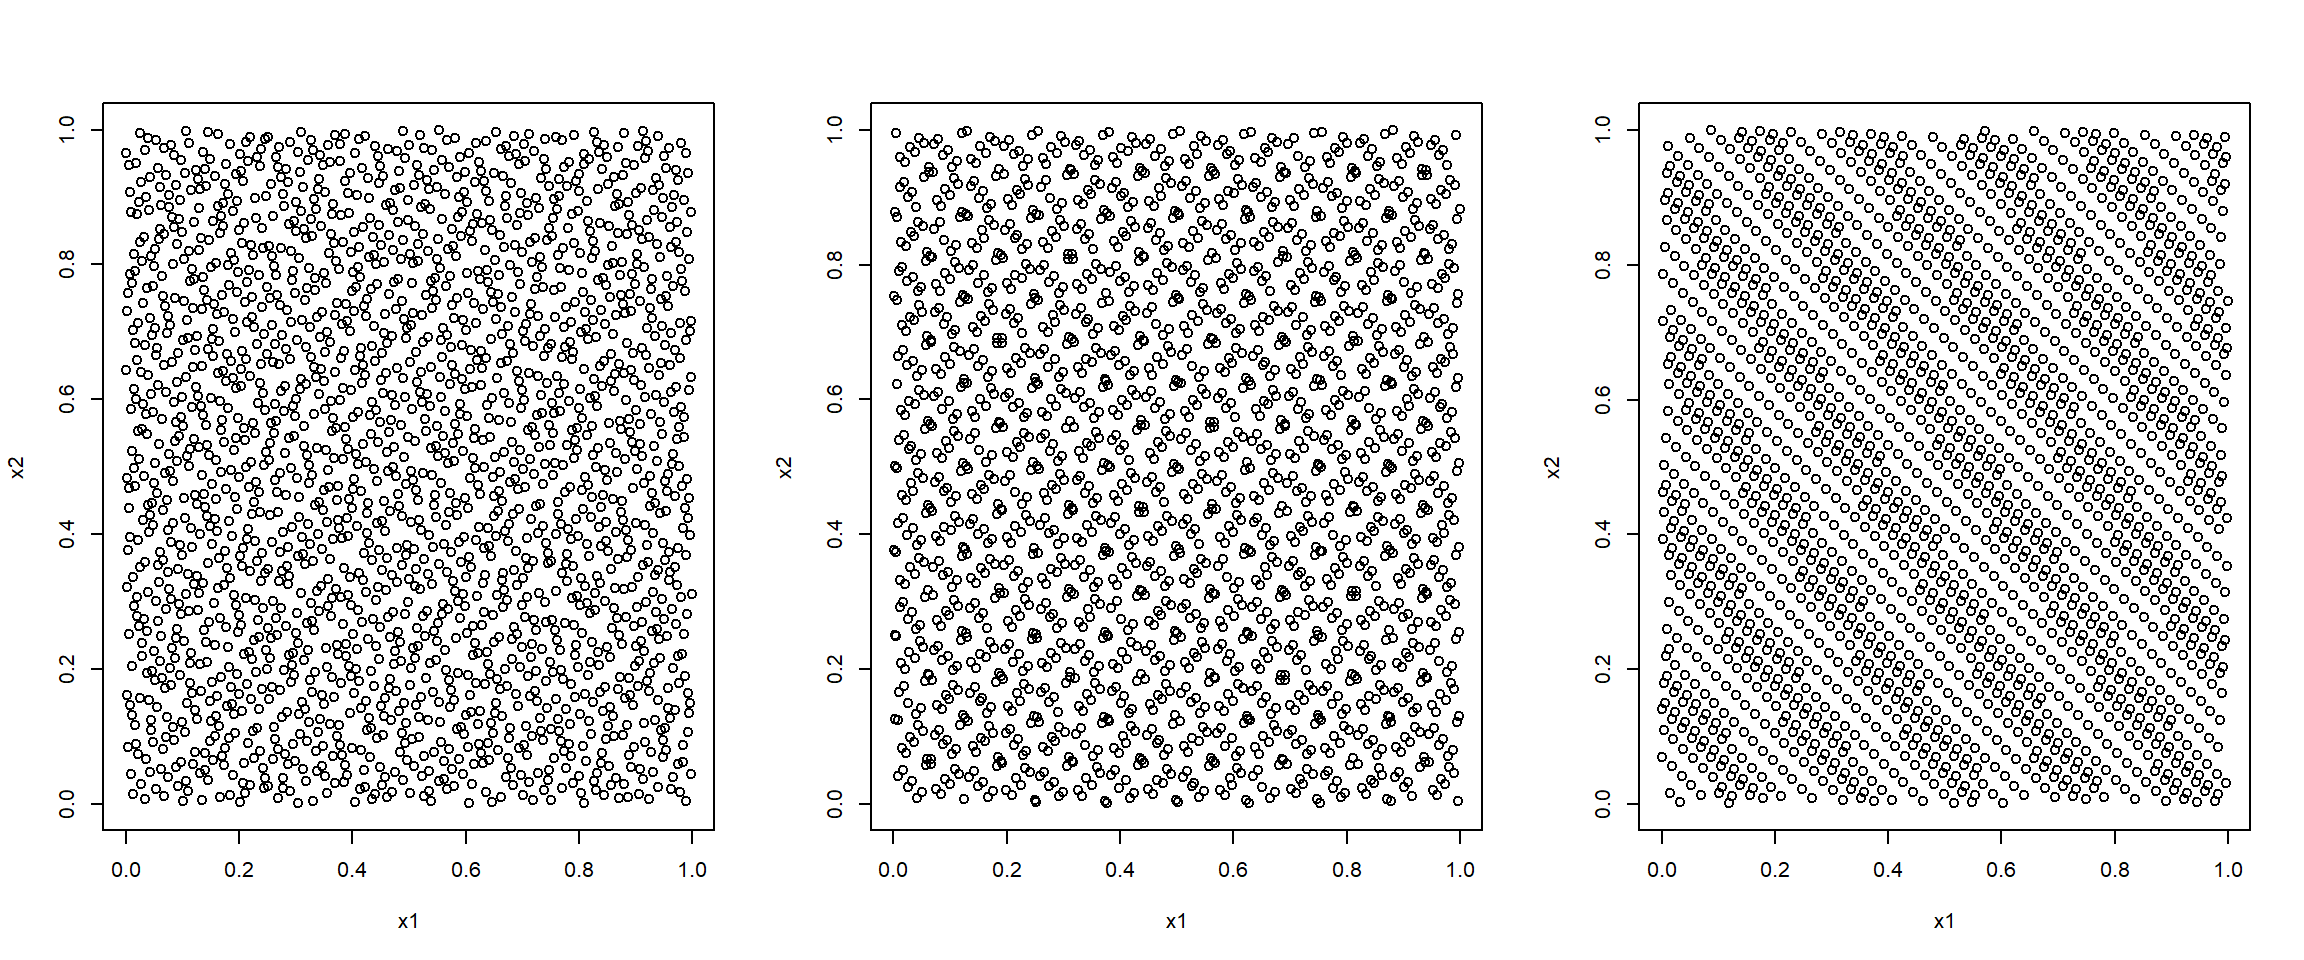
\includegraphics[width=1\linewidth]{01-Introduccion_files/figure-latex/randtoolbox-1} 

}

\caption{Secuencias cuasi-aleatorias bidimensionales obtenidas con los métodos de Halton (izquierda), Sobol (centro) y Torus (derecha).}\label{fig:randtoolbox}
\end{figure}

\begin{Shaded}
\begin{Highlighting}[]
\KeywordTok{par}\NormalTok{(par.old)}
\end{Highlighting}
\end{Shaded}

En este libro sólo consideraremos los números pseudoaleatorios y por comodidad se eliminará el prefijo ``pseudo'' en algunos casos.

\hypertarget{nuxfameros-pseudoaleatorios}{%
\section{Números pseudoaleatorios}\label{nuxfameros-pseudoaleatorios}}

La mayoría de los métodos de simulación se basan en la posibilidad de generar números pseudoaleatorios que imiten las propiedades de generaciones independientes de una distribución \(\mathcal{U}(0,1)\).

El procedimiento habitual para obtiener estas secuencias es emplear un algoritmo recursivo denominado \emph{generador}:

\[x_{i} = f\left( x_{i-1}, x_{i-2}, \cdots, x_{i-k}\right)\]

donde:

\begin{itemize}
\item
  \(k\) es el orden del generador.
\item
  \(\left( x_{0},x_{1},\cdots,x_{k-1}\right)\) es la \emph{semilla}
  (estado inicial).
\end{itemize}

El \emph{periodo} o \emph{longitud del ciclo} es la longitud de la secuencia antes de que vuelva a repetirse. Lo denotaremos por \(p\).

Los números de la sucesión serán predecibles, conociendo el algoritmo y la semilla.

\begin{itemize}
\item
  Sin embargo, si no se conociesen, \emph{no se debería poder distinguir} una serie de números pseudoaleatorios \emph{de una sucesión de números verdaderamente aleatoria} (utilizando recursos computacionales razonables).
\item
  En caso contrario esta predecibilidad puede dar lugar a serios
  problemas (e.g.~\url{http://eprint.iacr.org/2007/419}).
\end{itemize}

Como regla general, por lo menos mientras se está desarrollando un
programa, interesa \emph{fijar la semilla de aleatorización}.

\begin{itemize}
\item
  Permite la reproductibilidad de los resultados.
\item
  Facilita la depuración del código.
\end{itemize}

Todo generador de números pseudoaleatorios mínimamente aceptable
debe comportarse como si se tratase de una muestra genuina de datos
independientes de una \(\mathcal{U}(0,1)\).
Otras propiedades de interés serían:

\begin{itemize}
\item
  Reproducibilidad a partir de la semilla.
\item
  Periodo suficientemente largo.
\item
  Eficiencia (rapidez y requerimientos de memoria).
\item
  Portabilidad.
\item
  Generación de sub-secuencias (computación en paralelo).
\item
  Parsimonia\ldots{}
\end{itemize}

\begin{quote}
``\ldots{} random numbers should not be generated with a method chosen at random.''

--- Knuth, D.E. (TAOCP, 2002)
\end{quote}

Gran cantidad de algoritmos:

\begin{itemize}
\item
  Cuadrados medios, Lehmer\ldots{}
\item
  Congruenciales
\item
  Registros desfasados
\item
  Combinaciones
\item
  \ldots{}
\end{itemize}

Código fuente disponible en múltiples librerias:

\begin{itemize}
\item
  GNU Scientific Library (GSL):
  \href{http://www.gnu.org/software/gsl/manual/html_node/Random-Number-Generation.html}{http://www.gnu.org/software/gsl/manual}
\item
  StatLib: \url{http://lib.stat.cmu.edu}
\item
  Numerical recipes: \url{http://www.nrbook.com/nr3}
\item
  \url{http://random.mat.sbg.ac.at/software}
\item
  KISS (Keep It Simple Stupid / Small and Simple):
  \url{http://www.fortran.com/kiss.f90}
\item
  UNU.RAN (paquete \texttt{Runuran}):
  \url{http://statmath.wu.ac.at/unuran}
\item
  \ldots{}
\end{itemize}

Nos centraremos en los generadores congruenciales, descritos en la Sección \ref{gen-cong}.

\hypertarget{rrng}{%
\chapter{Números aleatorios en R}\label{rrng}}

La generación de números pseudoaleatorios en R es una de las mejores
disponibles en paquetes estadísticos.
Entre las herramientas en el paquete base de \texttt{R} estarían:

\begin{itemize}
\item
  \texttt{set.seed(entero)}: permite establecer la semilla (y el
  generador).
\item
  \texttt{RNGkind()}: selecciona el generador.
\item
  \texttt{rdistribución(n,...):} genera valores aleatorios de la
  correspondiente distribución.
  Por ejemplo, \texttt{runif(n,\ min\ =\ 0,\ max\ =\ 1)}, generaría \texttt{n} valores de una uniforme. Se puede acceder al listado completo de las funciones disponibles en el paquete \texttt{stats} mediante el comando \texttt{?distributions}.
\item
  \texttt{sample()}: genera muestras aleatorias de variables discretas y permutaciones (se tratará en el Capítulo \ref{discretas}).
\item
  \texttt{simulate()}: genera realizaciones de la respuesta de un modelo ajustado.
\end{itemize}

Además están disponibles otros paquetes que implementan distribuciones adicionales (ver \href{https://cran.r-project.org/view=Distributions}{CRAN Task View: Probability Distributions}).
Entre ellos podríamos destacar los paquetes \href{http://distr.r-forge.r-project.org}{\texttt{distr}} (clases S4; con extensiones en otros paquetes) y \href{https://alan-turing-institute.github.io/distr6/index.html}{\texttt{distr6}} (clases R6).

La semilla se almacena (en \texttt{globalenv}) en \texttt{.Random.seed}; es un vector
de enteros cuya dimensión depende del tipo de generador:

\begin{itemize}
\item
  No debe ser modificado manualmente; se guarda con el entorno
  de trabajo.
\item
  Si no se especifica con \texttt{set.seed} (o no existe) se genera a
  partir del reloj del sistema.
\end{itemize}

\begin{remark}
\iffalse{} {Nota: } \fi{}Puede ser recomendable (para depurar) almacenarla antes de generar simulaciones, e.g.~
\texttt{semilla\ \textless{}-\ .Random.seed}.
\end{remark}

En la mayoría de los ejemplos de este libro se generan todos los valores de una vez,
se guardan y se procesan vectorialmente (normalmente empleando la función \texttt{apply}).
En problemas mas complejos, en los que no es necesario almacenar todas las simulaciones,
puede ser preferible emplear un bucle para generar y procesar cada simulación iterativamente.
Por ejemplo podríamos emplear el siguiente esquema:

\begin{Shaded}
\begin{Highlighting}[]
\CommentTok{# Fijar semilla}
\KeywordTok{set.seed}\NormalTok{(}\DecValTok{1}\NormalTok{)}
\ControlFlowTok{for}\NormalTok{ (isim }\ControlFlowTok{in} \DecValTok{1}\OperatorTok{:}\NormalTok{nsim) \{}
\NormalTok{  seed <-}\StringTok{ }\NormalTok{.Random.seed}
  \CommentTok{# Si se produce un error, podremos depurarlo ejecutando:}
  \CommentTok{#  .Random.seed <- seed}
\NormalTok{  ...}
  \CommentTok{# Generar valores pseudoaleatorios}
\NormalTok{  ...}
\NormalTok{\}}
\end{Highlighting}
\end{Shaded}

o alternativamente fijar la semilla en cada iteración, por ejemplo:

\begin{Shaded}
\begin{Highlighting}[]
\ControlFlowTok{for}\NormalTok{ (isim }\ControlFlowTok{in} \DecValTok{1}\OperatorTok{:}\NormalTok{nsim) \{}
  \KeywordTok{set.seed}\NormalTok{(isim)}
\NormalTok{  ...}
  \CommentTok{# Generar valores pseudoaleatorios}
\NormalTok{  ...}
\NormalTok{\}}
\end{Highlighting}
\end{Shaded}

Hay que tener en cuenta que \texttt{.Random.seed} se almacena en el entorno de trabajo\ldots{}

\hypertarget{opciones}{%
\section{Opciones}\label{opciones}}

La función \texttt{RNGkind(kind\ =\ NULL,\ normal.kind\ =\ NULL)} permite
seleccionar el tipo de generador (en negrita los valores por defecto):

\begin{itemize}
\item
  \texttt{kind} especifica el generador aleatorio:

  \begin{itemize}
  \item
    ``Wichmann-Hill'': Ciclo \(6.9536\times10^{12}\)
  \item
    ``Marsaglia-Multicarry'': Ciclo mayor de \(2^{60}\)
  \item
    ``Super-Duper'': Ciclo aprox. \(4.6\times10^{18}\) (S-PLUS)
  \item
    \textbf{``Mersenne-Twister''}: Ciclo \(2^{19937}-1\) y equidistribution
    en 623 dimensiones.
  \item
    ``Knuth-TAOCP-2002'': Ciclo aprox. \(2^{129}\).
  \item
    ``Knuth-TAOCP''
  \item
    ``user-supplied''
  \end{itemize}
\item
  \texttt{normal.kind} selecciona el método de generación de normales
  (se tratará más adelante).
  ``Kinderman-Ramage'', ``Buggy Kinderman-Ramage'',
  ``Ahrens-Dieter'', ``Box-Muller'', \textbf{``Inversion''} , o ``user-supplied''
\end{itemize}

\hypertarget{paquetes-de-r}{%
\section{Paquetes de R}\label{paquetes-de-r}}

Otros paquetes de R que pueden ser de interés:

\begin{itemize}
\item
  \texttt{setRNG} contiene herramientas que facilitan operar con la semilla
  (dentro de funciones,\ldots).
\item
  \texttt{random} permite la descarga de números ``true random'' desde \href{https://www.random.org}{RANDOM.ORG}.
\item
  \texttt{randtoolbox} implementa generadores más recientes (\texttt{rngWELL}) y
  generación de secuencias cuasi-aleatorias.
\item
  \texttt{RDieHarder} implementa diversos contrastes para el análisis de la
  calidad de un generador y varios generadores.
\item
  \href{http://statmath.wu.ac.at/unuran}{\texttt{Runuran}} interfaz para la librería UNU.RAN para la
  generación (automática) de variables aleatorias no uniformes (ver Hörmann et al., 2004).
\item
  \texttt{rsprng}, \texttt{rstream} y \texttt{rlecuyer} implementan la generación de múltiples
  secuencias (para programación paralela).
\item
  \texttt{gls}, \texttt{rngwell19937}, \texttt{randaes}, \texttt{SuppDists}, \texttt{lhs}, \texttt{mc2d},
  \texttt{fOptions}, \ldots{}
\end{itemize}

\hypertarget{ejercicios}{%
\section{Ejercicios}\label{ejercicios}}

\begin{exercise}
\protect\hypertarget{exr:simpi}{}{\label{exr:simpi} }
\end{exercise}

Sea \((X,Y)\) es un vector aleatorio con distribución uniforme en el
cuadrado \([-1,1]\times\lbrack-1,1]\) de área 4.

\begin{enumerate}
\def\labelenumi{\alph{enumi})}
\item
  Aproximar mediante simulación \(P\left(X + Y \leq 0 \right)\) y
  compararla con la probabilidad teórica (obtenida aplicando la
  regla de Laplace \(\frac{\text{área favorable}}{\text{área posible}}\)).

  Generamos \texttt{nsim\ =\ 10000} valores del proceso bidimensional:

\begin{Shaded}
\begin{Highlighting}[]
\KeywordTok{set.seed}\NormalTok{(}\DecValTok{1}\NormalTok{)}
\NormalTok{nsim <-}\StringTok{ }\DecValTok{10000}
\NormalTok{x <-}\StringTok{ }\KeywordTok{runif}\NormalTok{(nsim, }\DecValTok{-1}\NormalTok{, }\DecValTok{1}\NormalTok{)}
\NormalTok{y <-}\StringTok{ }\KeywordTok{runif}\NormalTok{(nsim, }\DecValTok{-1}\NormalTok{, }\DecValTok{1}\NormalTok{)}
\end{Highlighting}
\end{Shaded}

  La probabilidad teórica es 1/2 y la aproximación por simulación es la frecuencia relativa del suceso en los valores generados (para calcularla podemos aprovechar que R maneja internamente los valores lógicos como 1, \texttt{TRUE}, y 0, \texttt{FALSE}):

\begin{Shaded}
\begin{Highlighting}[]
\NormalTok{indice <-}\StringTok{ }\NormalTok{(x}\OperatorTok{+}\NormalTok{y }\OperatorTok{<}\StringTok{ }\DecValTok{0}\NormalTok{)}
\KeywordTok{sum}\NormalTok{(indice)}\OperatorTok{/}\NormalTok{nsim}
\end{Highlighting}
\end{Shaded}

\begin{verbatim}
## [1] 0.4996
\end{verbatim}

  Alternativamente (la frecuencia relativa es un caso particular de la media) se puede obtener de forma más simple como:

\begin{Shaded}
\begin{Highlighting}[]
\KeywordTok{mean}\NormalTok{(indice)}
\end{Highlighting}
\end{Shaded}

\begin{verbatim}
## [1] 0.4996
\end{verbatim}
\item
  Aproximar el valor de \(\pi\) mediante simulación a partir de
  \(P\left( X^2 +Y^2 \leq 1 \right)\).

\begin{Shaded}
\begin{Highlighting}[]
\KeywordTok{set.seed}\NormalTok{(}\DecValTok{1}\NormalTok{)}
\NormalTok{n <-}\StringTok{ }\DecValTok{10000}
\NormalTok{x <-}\StringTok{ }\KeywordTok{runif}\NormalTok{(n, }\DecValTok{-1}\NormalTok{, }\DecValTok{1}\NormalTok{)}
\NormalTok{y <-}\StringTok{ }\KeywordTok{runif}\NormalTok{(n, }\DecValTok{-1}\NormalTok{, }\DecValTok{1}\NormalTok{)}
\NormalTok{indice <-}\StringTok{ }\NormalTok{(x}\OperatorTok{^}\DecValTok{2}\OperatorTok{+}\NormalTok{y}\OperatorTok{^}\DecValTok{2} \OperatorTok{<}\StringTok{ }\DecValTok{1}\NormalTok{)}
\KeywordTok{mean}\NormalTok{(indice)}
\end{Highlighting}
\end{Shaded}

\begin{verbatim}
## [1] 0.7806
\end{verbatim}

\begin{Shaded}
\begin{Highlighting}[]
\NormalTok{pi}\OperatorTok{/}\DecValTok{4}
\end{Highlighting}
\end{Shaded}

\begin{verbatim}
## [1] 0.7853982
\end{verbatim}

\begin{Shaded}
\begin{Highlighting}[]
\NormalTok{pi_aprox <-}\StringTok{ }\DecValTok{4}\OperatorTok{*}\KeywordTok{mean}\NormalTok{(indice)}
\NormalTok{pi_aprox}
\end{Highlighting}
\end{Shaded}

\begin{verbatim}
## [1] 3.1224
\end{verbatim}

  Generamos el correspondiente gráfico (ver Figura \ref{fig:simpiplot}) (los puntos con color negro tienen distribución uniforme en el círculo unidad; esto está relacionado con el método de aceptación-rechazo, ver \ref{exm:ar-esfera}, o con el denominado método \emph{hit-or-miss}).

\begin{Shaded}
\begin{Highlighting}[]
\CommentTok{# Colores y símbolos dependiendo de si el índice correspondiente es verdadero:}
\NormalTok{color <-}\StringTok{ }\KeywordTok{ifelse}\NormalTok{(indice, }\StringTok{"black"}\NormalTok{, }\StringTok{"red"}\NormalTok{) }
\NormalTok{simbolo <-}\StringTok{ }\KeywordTok{ifelse}\NormalTok{(indice, }\DecValTok{1}\NormalTok{, }\DecValTok{4}\NormalTok{)}
\KeywordTok{plot}\NormalTok{(x, y, }\DataTypeTok{pch =}\NormalTok{ simbolo, }\DataTypeTok{col =}\NormalTok{ color, }
     \DataTypeTok{xlim =} \KeywordTok{c}\NormalTok{(}\OperatorTok{-}\DecValTok{1}\NormalTok{, }\DecValTok{1}\NormalTok{), }\DataTypeTok{ylim =} \KeywordTok{c}\NormalTok{(}\OperatorTok{-}\DecValTok{1}\NormalTok{, }\DecValTok{1}\NormalTok{), }\DataTypeTok{xlab=}\StringTok{"X"}\NormalTok{, }\DataTypeTok{ylab=}\StringTok{"Y"}\NormalTok{, }\DataTypeTok{asp =} \DecValTok{1}\NormalTok{) }
     \CommentTok{# asp = 1 para dibujar circulo}
\KeywordTok{symbols}\NormalTok{(}\DecValTok{0}\NormalTok{, }\DecValTok{0}\NormalTok{, }\DataTypeTok{circles =} \DecValTok{1}\NormalTok{, }\DataTypeTok{inches =} \OtherTok{FALSE}\NormalTok{, }\DataTypeTok{add =} \OtherTok{TRUE}\NormalTok{)}
\KeywordTok{symbols}\NormalTok{(}\DecValTok{0}\NormalTok{, }\DecValTok{0}\NormalTok{, }\DataTypeTok{squares =} \DecValTok{2}\NormalTok{, }\DataTypeTok{inches =} \OtherTok{FALSE}\NormalTok{, }\DataTypeTok{add =} \OtherTok{TRUE}\NormalTok{)}
\end{Highlighting}
\end{Shaded}

  \begin{figure}[!htb]

  {\centering 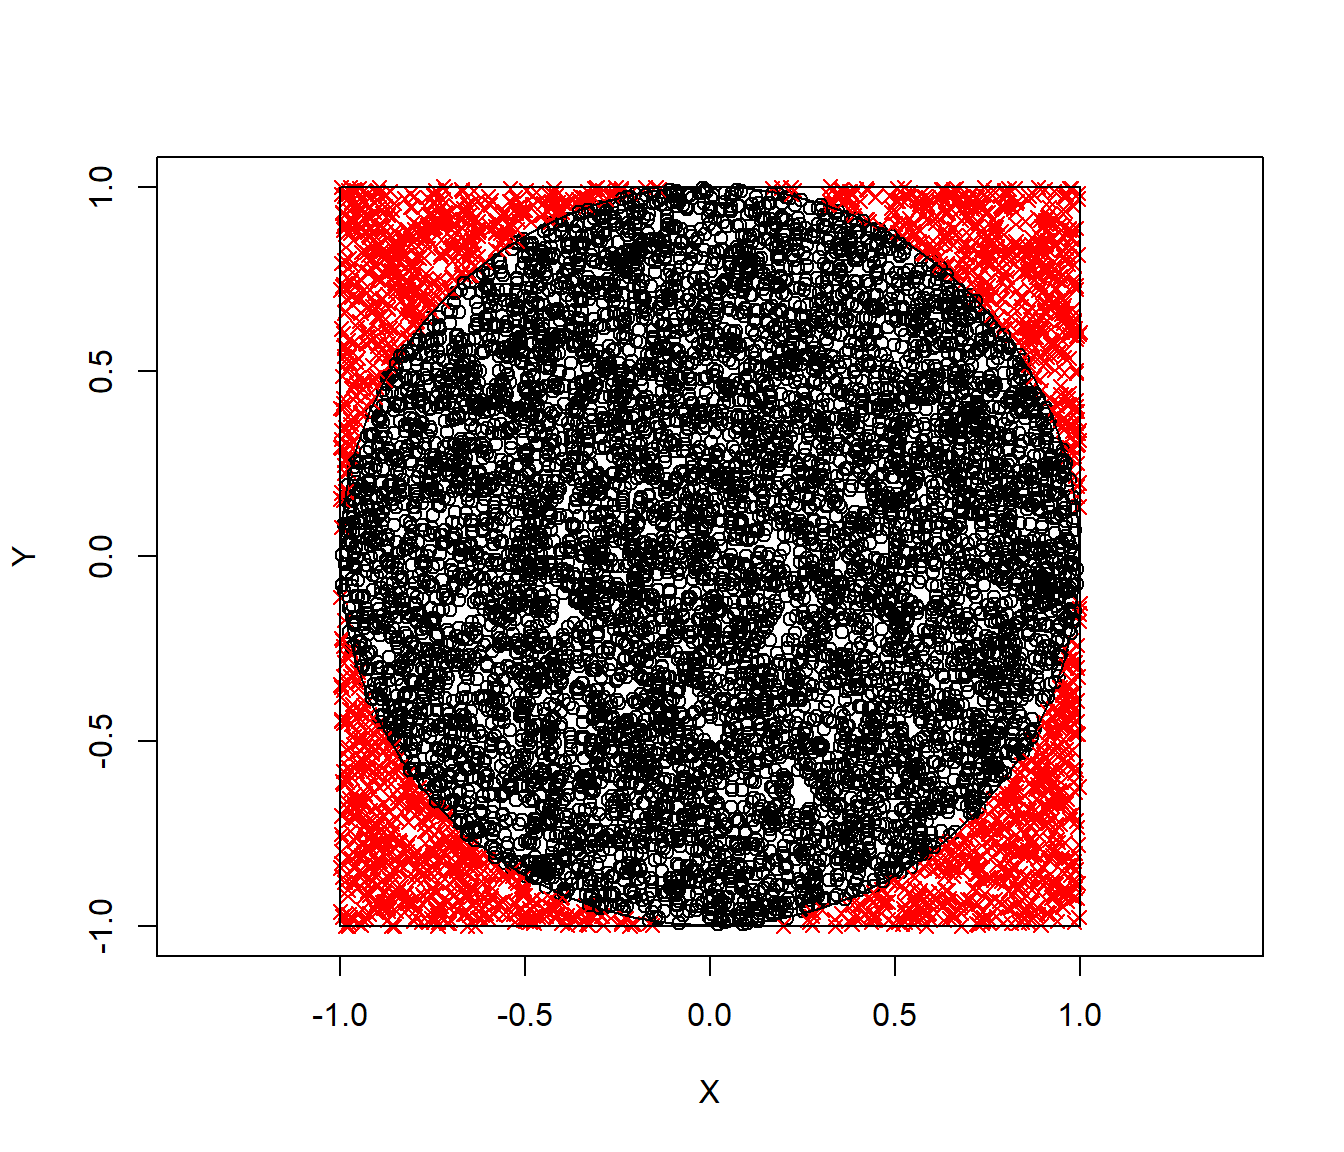
\includegraphics[width=0.7\linewidth]{02-Numeros_aleatorios_R_files/figure-latex/simpiplot-1} 

  }

  \caption{Valores generados con distribución uniforme bidimensional, con colores y símbolos indicando si están dentro del círculo unidad.}\label{fig:simpiplot}
  \end{figure}
\end{enumerate}

\begin{exercise}[Experimento de Bernoulli]
\protect\hypertarget{exr:bernouilli}{}{\label{exr:bernouilli} \iffalse (Experimento de Bernoulli) \fi{} }
\end{exercise}
Consideramos el experimento de Bernoulli consistente en el
lanzamiento de una moneda.

\begin{enumerate}
\def\labelenumi{\alph{enumi})}
\item
  Empleando la función \texttt{sample}, obtener 1000 simulaciones del
  lanzamiento de una moneda \texttt{(0\ =\ cruz,\ 1\ =\ cara)}, suponiendo que
  no está trucada. Aproximar la probabilidad de cara a partir de
  las simulaciones.

\begin{Shaded}
\begin{Highlighting}[]
\KeywordTok{set.seed}\NormalTok{(}\DecValTok{1}\NormalTok{)}
\NormalTok{nsim <-}\StringTok{ }\DecValTok{10000}
\NormalTok{x <-}\StringTok{ }\KeywordTok{sample}\NormalTok{(}\KeywordTok{c}\NormalTok{(}\DataTypeTok{cara =} \DecValTok{1}\NormalTok{, }\DataTypeTok{cruz =} \DecValTok{0}\NormalTok{), nsim, }\DataTypeTok{replace =} \OtherTok{TRUE}\NormalTok{, }\DataTypeTok{prob =} \KeywordTok{c}\NormalTok{(}\FloatTok{0.5}\NormalTok{,}\FloatTok{0.5}\NormalTok{))}
\KeywordTok{mean}\NormalTok{(x)}
\end{Highlighting}
\end{Shaded}

\begin{verbatim}
## [1] 0.4953
\end{verbatim}

\begin{Shaded}
\begin{Highlighting}[]
\KeywordTok{barplot}\NormalTok{(}\DecValTok{100}\OperatorTok{*}\KeywordTok{table}\NormalTok{(x)}\OperatorTok{/}\NormalTok{nsim, }\DataTypeTok{ylab =} \StringTok{"Porcentaje"}\NormalTok{) }\CommentTok{# Representar porcentajes }
\end{Highlighting}
\end{Shaded}

  \begin{figure}[!htb]

  {\centering 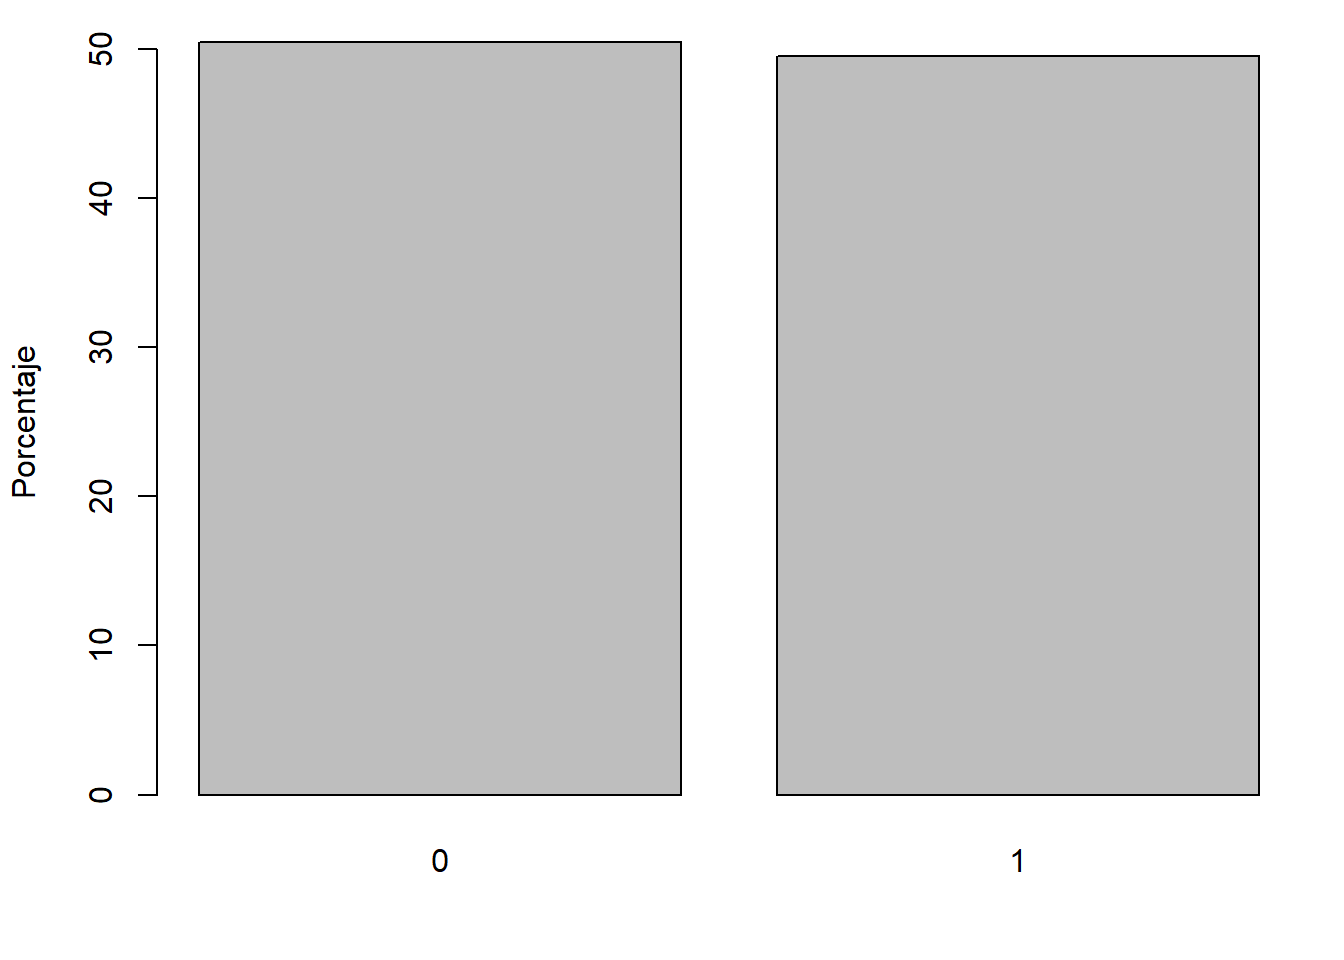
\includegraphics[width=0.7\linewidth]{02-Numeros_aleatorios_R_files/figure-latex/simberplot-1} 

  }

  \caption{Frecuencias relativas de los valores generados con distribución Bernoulli (aproximaciones por simulación de las probabilidades teóricas).}\label{fig:simberplot}
  \end{figure}
\item
  En R pueden generarse valores de la distribución de Bernoulli
  mediante la función \texttt{rbinom(nsim,\ size=1,\ prob)}. Generar un
  gráfico de lineas considerando en el eje \(X\) el número de
  lanzamientos (de 1 a 10000) y en el eje \(Y\) la frecuencia
  relativa del suceso cara (puede ser recomendable emplear la
  función \texttt{cumsum}).

\begin{Shaded}
\begin{Highlighting}[]
\KeywordTok{set.seed}\NormalTok{(}\DecValTok{1}\NormalTok{)}
\NormalTok{nsim <-}\StringTok{ }\DecValTok{1000}
\NormalTok{p <-}\StringTok{ }\FloatTok{0.4}
\NormalTok{x <-}\StringTok{ }\KeywordTok{rbinom}\NormalTok{(nsim, }\DataTypeTok{size =} \DecValTok{1}\NormalTok{, }\DataTypeTok{prob =}\NormalTok{ p) }\CommentTok{# Simulamos una Bernouilli}
\NormalTok{n <-}\StringTok{ }\DecValTok{1}\OperatorTok{:}\NormalTok{nsim}
\CommentTok{# Alternativa programación: x <- runif(nsim) < p}
\KeywordTok{mean}\NormalTok{(x)}
\end{Highlighting}
\end{Shaded}

\begin{verbatim}
## [1] 0.394
\end{verbatim}

\begin{Shaded}
\begin{Highlighting}[]
\KeywordTok{plot}\NormalTok{(n, }\KeywordTok{cumsum}\NormalTok{(x)}\OperatorTok{/}\NormalTok{n, }\DataTypeTok{type=}\StringTok{"l"}\NormalTok{, }\DataTypeTok{ylab=}\StringTok{"Proporción de caras"}\NormalTok{, }
     \DataTypeTok{xlab=}\StringTok{"Número de lanzamientos"}\NormalTok{, }\DataTypeTok{ylim=}\KeywordTok{c}\NormalTok{(}\DecValTok{0}\NormalTok{,}\DecValTok{1}\NormalTok{))}
\KeywordTok{abline}\NormalTok{(}\DataTypeTok{h=}\NormalTok{p, }\DataTypeTok{lty=}\DecValTok{2}\NormalTok{, }\DataTypeTok{col=}\StringTok{"red"}\NormalTok{)}
\end{Highlighting}
\end{Shaded}

  \begin{figure}[!htb]

  {\centering 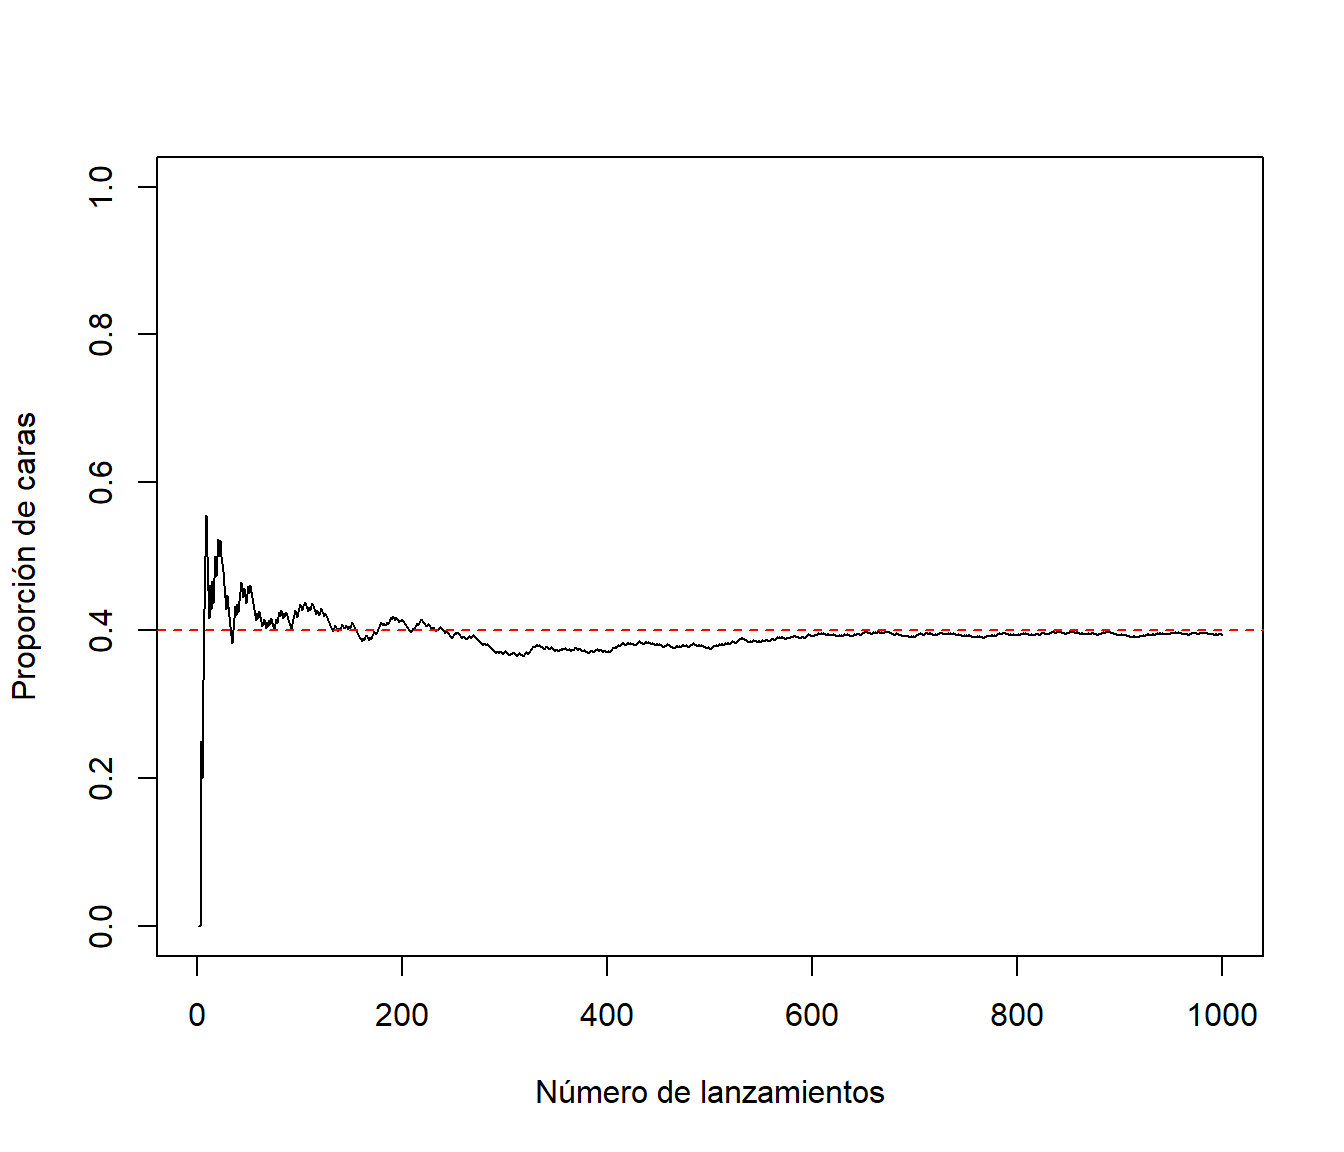
\includegraphics[width=0.7\linewidth]{02-Numeros_aleatorios_R_files/figure-latex/simberconv-1} 

  }

  \caption{Gráfico de convergencia de la aproximación por simulación a la probabilidad teórica.}\label{fig:simberconv}
  \end{figure}
\end{enumerate}

\begin{exercise}[Simulación de un circuito]
\protect\hypertarget{exr:circuito}{}{\label{exr:circuito} \iffalse (Simulación de un circuito) \fi{} }
\end{exercise}
Simular el paso de corriente a través del siguiente circuito, donde
figuran las probabilidades de que pase corriente por cada uno de los
interruptores:

\begin{center}\includegraphics[width=0.5\linewidth]{images/circuito2} \end{center}

Considerar que cada interruptor es una variable aleatoria de Bernoulli independiente
para simular 1000 valores de cada una de ellas.

\begin{remark}
\iffalse{} {Nota: } \fi{}R maneja internamente los valores lógicos como 1 (\texttt{TRUE}) y 0 (\texttt{FALSE}).
Recíprocamente, cualquier número puede ser tratado como lógico (al estilo de C).
El entero 0 es equivalente a \texttt{FALSE} y cualquier entero distinto de 0 a \texttt{TRUE}.
\end{remark}

\begin{Shaded}
\begin{Highlighting}[]
\KeywordTok{set.seed}\NormalTok{(}\DecValTok{1}\NormalTok{)}
\NormalTok{nsim <-}\StringTok{ }\DecValTok{10000}
\NormalTok{x1 <-}\StringTok{ }\KeywordTok{rbinom}\NormalTok{(nsim, }\DataTypeTok{size=}\DecValTok{1}\NormalTok{, }\DataTypeTok{prob=}\FloatTok{0.9}\NormalTok{)}
\NormalTok{x2 <-}\StringTok{ }\KeywordTok{rbinom}\NormalTok{(nsim, }\DataTypeTok{size=}\DecValTok{1}\NormalTok{, }\DataTypeTok{prob=}\FloatTok{0.8}\NormalTok{)}
\NormalTok{z1 <-}\StringTok{ }\NormalTok{x1 }\OperatorTok{|}\StringTok{ }\NormalTok{x2   }\CommentTok{# Operador lógico "O"}
\NormalTok{x3 <-}\StringTok{ }\KeywordTok{rbinom}\NormalTok{(nsim, }\DataTypeTok{size=}\DecValTok{1}\NormalTok{, }\DataTypeTok{prob=}\FloatTok{0.6}\NormalTok{)}
\NormalTok{x4 <-}\StringTok{ }\KeywordTok{rbinom}\NormalTok{(nsim, }\DataTypeTok{size=}\DecValTok{1}\NormalTok{, }\DataTypeTok{prob=}\FloatTok{0.5}\NormalTok{)}
\NormalTok{z2 <-}\StringTok{ }\NormalTok{x3 }\OperatorTok{|}\StringTok{ }\NormalTok{x4}
\NormalTok{z3 <-}\StringTok{ }\NormalTok{z1 }\OperatorTok{|}\StringTok{ }\NormalTok{z2}
\NormalTok{x5 <-}\StringTok{ }\KeywordTok{rbinom}\NormalTok{(nsim, }\DataTypeTok{size=}\DecValTok{1}\NormalTok{, }\DataTypeTok{prob=}\FloatTok{0.7}\NormalTok{)}
\NormalTok{fin <-}\StringTok{ }\NormalTok{z3 }\OperatorTok{&}\StringTok{ }\NormalTok{x5  }\CommentTok{# Operador lógico "Y"}
\KeywordTok{mean}\NormalTok{(fin)}
\end{Highlighting}
\end{Shaded}

\begin{verbatim}
## [1] 0.6918
\end{verbatim}

\begin{exercise}[El problema del Caballero de Méré]
\protect\hypertarget{exr:mere}{}{\label{exr:mere} \iffalse (El problema del Caballero de Méré) \fi{} }
\end{exercise}
En 1651, el Caballero de Méré le planteó a Pascal una pregunta
relacionada con las apuestas y los juegos de azar: ¿es ventajoso
apostar a que en cuatro lanzamientos de un dado se obtiene al menos
un seis? Este problema generó una fructífera correspondencia entre
Pascal y Fermat que se considera, simbólicamente, como el nacimiento
del Cálculo de Probabilidades.

\begin{enumerate}
\def\labelenumi{\alph{enumi})}
\item
  Escribir una función que simule el lanzamiento de \(n\) dados. El
  parámetro de entrada es el número de lanzamientos \(n\), que toma
  el valor 4 por defecto, y la salida debe ser \texttt{TRUE} si se
  obtiene al menos un 6 y \texttt{FALSE} en caso contrario.

\begin{Shaded}
\begin{Highlighting}[]
\NormalTok{deMere <-}\StringTok{ }\ControlFlowTok{function}\NormalTok{(}\DataTypeTok{n =} \DecValTok{4}\NormalTok{)\{}
\NormalTok{  lanz <-}\StringTok{ }\KeywordTok{sample}\NormalTok{(}\DecValTok{1}\OperatorTok{:}\DecValTok{6}\NormalTok{, }\DataTypeTok{replace=}\OtherTok{TRUE}\NormalTok{, }\DataTypeTok{size=}\NormalTok{n)}
  \KeywordTok{return}\NormalTok{(}\DecValTok{6} \OperatorTok\StringTok{ }\NormalTok{lanz)}
\NormalTok{\}}

\NormalTok{n <-}\StringTok{ }\DecValTok{4}
\NormalTok{lanz <-}\StringTok{ }\KeywordTok{sample}\NormalTok{(}\DecValTok{1}\OperatorTok{:}\DecValTok{6}\NormalTok{, }\DataTypeTok{replace=}\OtherTok{TRUE}\NormalTok{, }\DataTypeTok{size=}\NormalTok{n)}
\NormalTok{lanz}
\end{Highlighting}
\end{Shaded}

\begin{verbatim}
## [1] 3 5 1 6
\end{verbatim}

\begin{Shaded}
\begin{Highlighting}[]
\DecValTok{6} \OperatorTok\StringTok{ }\NormalTok{lanz}
\end{Highlighting}
\end{Shaded}

\begin{verbatim}
## [1] TRUE
\end{verbatim}
\item
  Utilizar la función anterior para simular \(nsim=10000\) jugadas
  de este juego y calcular la proporción de veces que se gana la
  apuesta (obtener al menos un 6 en \(n\) lanzamientos), usando
  \(n=4\). Comparar el resultado con la probabilidad teórica
  \(1-(5/6)^{n}\).

\begin{Shaded}
\begin{Highlighting}[]
\KeywordTok{set.seed}\NormalTok{(}\DecValTok{1}\NormalTok{)}
\NormalTok{n <-}\StringTok{ }\DecValTok{4}
\NormalTok{nsim <-}\StringTok{ }\DecValTok{10000}
\KeywordTok{mean}\NormalTok{(}\KeywordTok{replicate}\NormalTok{(nsim, }\KeywordTok{deMere}\NormalTok{(n)))}
\end{Highlighting}
\end{Shaded}

\begin{verbatim}
## [1] 0.5148
\end{verbatim}

\begin{Shaded}
\begin{Highlighting}[]
\DecValTok{1}\OperatorTok{-}\NormalTok{(}\DecValTok{5}\OperatorTok{/}\DecValTok{6}\NormalTok{)}\OperatorTok{^}\NormalTok{n}
\end{Highlighting}
\end{Shaded}

\begin{verbatim}
## [1] 0.5177469
\end{verbatim}
\end{enumerate}

\hypertarget{tiempo-de-cpu}{%
\section{Tiempo de CPU}\label{tiempo-de-cpu}}

La velocidad del generador suele ser una característica importante.
Para evaluar el rendimiento están disponibles en \texttt{R} distintas herramientas:

\begin{itemize}
\item
  \texttt{proc.time()}: permite obtener tiempo de computación real y de
  CPU.

\begin{verbatim}
tini <- proc.time()
# Código a evaluar
tiempo <- proc.time() - tini
\end{verbatim}
\item
  \texttt{system.time(expresión)}: muestra el tiempo de computación (real y
  de CPU) de expresión.
\item
  \texttt{Rprof(fichero)}: permite evaluar el rendimiento muestreando la pila
  en intervalos para determinar en que funciones se emplea el tiempo
  de computación (de utilidad para optimizar la
  velocidad).\texttt{Rprof(NULL)}: desactiva el
  muestreo.\texttt{summaryRprof(fichero)}: muestra los resultados.
\end{itemize}

\hypertarget{utilidades-tiempo-de-cpu}{%
\subsection{Utilidades tiempo de CPU}\label{utilidades-tiempo-de-cpu}}

Por ejemplo, podríamos emplear las siguientes funciones para
ir midiendo los tiempos de CPU durante una simulación:

\begin{Shaded}
\begin{Highlighting}[]
\NormalTok{CPUtimeini <-}\StringTok{ }\ControlFlowTok{function}\NormalTok{() \{}
\NormalTok{  .tiempo.ini <<-}\StringTok{ }\KeywordTok{proc.time}\NormalTok{()}
\NormalTok{  .tiempo.last <<-}\StringTok{ }\NormalTok{.tiempo.ini}
\NormalTok{\}}

\NormalTok{CPUtimeprint <-}\StringTok{ }\ControlFlowTok{function}\NormalTok{() \{}
\NormalTok{  tmp <-}\StringTok{ }\KeywordTok{proc.time}\NormalTok{()}
  \KeywordTok{cat}\NormalTok{(}\StringTok{"}\CharTok{\textbackslash{}n}\StringTok{Tiempo última operación:}\CharTok{\textbackslash{}n}\StringTok{"}\NormalTok{)}
  \KeywordTok{print}\NormalTok{(tmp}\OperatorTok{-}\NormalTok{.tiempo.last)}
  \KeywordTok{cat}\NormalTok{(}\StringTok{"Tiempo total operación:}\CharTok{\textbackslash{}n}\StringTok{"}\NormalTok{)}
  \KeywordTok{print}\NormalTok{(tmp}\OperatorTok{-}\NormalTok{.tiempo.ini)}
\NormalTok{  .tiempo.last <<-}\StringTok{ }\NormalTok{tmp}
\NormalTok{\}}
\end{Highlighting}
\end{Shaded}

Llamando a \texttt{CPUtimeini()} donde se quiere empezar a contar,
y a \texttt{CPUtimeprint()} para imprimir el tiempo total
y el tiempo desde la última llamada a una de estas funciones.
Ejemplo:

\begin{Shaded}
\begin{Highlighting}[]
\NormalTok{funtest <-}\StringTok{ }\ControlFlowTok{function}\NormalTok{(n) }\KeywordTok{median}\NormalTok{(}\KeywordTok{runif}\NormalTok{(n)) }\CommentTok{# Función de prueba...}
\KeywordTok{CPUtimeini}\NormalTok{()}
\KeywordTok{funtest}\NormalTok{(}\DecValTok{1000000}\NormalTok{)}
\end{Highlighting}
\end{Shaded}

\begin{verbatim}
## [1] 0.5003313
\end{verbatim}

\begin{Shaded}
\begin{Highlighting}[]
\KeywordTok{CPUtimeprint}\NormalTok{()}
\end{Highlighting}
\end{Shaded}

\begin{verbatim}
## 
## Tiempo última operación:
##    user  system elapsed 
##    0.13    0.00    0.13 
## Tiempo total operación:
##    user  system elapsed 
##    0.13    0.00    0.13
\end{verbatim}

\begin{Shaded}
\begin{Highlighting}[]
\KeywordTok{funtest}\NormalTok{(}\DecValTok{1000}\NormalTok{)}
\end{Highlighting}
\end{Shaded}

\begin{verbatim}
## [1] 0.5050682
\end{verbatim}

\begin{Shaded}
\begin{Highlighting}[]
\KeywordTok{CPUtimeprint}\NormalTok{()}
\end{Highlighting}
\end{Shaded}

\begin{verbatim}
## 
## Tiempo última operación:
##    user  system elapsed 
##    0.03    0.00    0.03 
## Tiempo total operación:
##    user  system elapsed 
##    0.16    0.00    0.16
\end{verbatim}

\hypertarget{paquetes-de-r-1}{%
\subsection{Paquetes de R}\label{paquetes-de-r-1}}

Por ejemplo, se puede emplear la función \href{https://rubenfcasal.github.io/npsp/reference/cpu.time.html}{\texttt{cpu.time()}} del paquete \texttt{npsp}:

\begin{itemize}
\item
  Call \texttt{cpu.time(restart\ =\ TRUE)} where you want to start counting.
\item
  Call \texttt{cpu.time()} to print/get total and/or partial (since the last call
  to this function) real and CPU times.
\end{itemize}

Fichero \emph{\href{https://github.com/rubenfcasal/npsp/blob/master/R/cpu.time.R}{cpu.time.R}}:

\begin{Shaded}
\begin{Highlighting}[]
\CommentTok{# CPU time utilities}
\CommentTok{# ------------------}

\CommentTok{#' @rdname npsp-internals}
\CommentTok{#' @keywords internal}
\CommentTok{#' @export}
\NormalTok{.cpu.time.ini <-}\StringTok{ }\ControlFlowTok{function}\NormalTok{() \{}
\NormalTok{    time.ini <-}\StringTok{ }\KeywordTok{structure}\NormalTok{(}\KeywordTok{rep}\NormalTok{(}\DecValTok{0}\NormalTok{, }\DecValTok{5}\NormalTok{), }\DataTypeTok{.Names =} \KeywordTok{c}\NormalTok{(}\StringTok{"user.self"}\NormalTok{, }\StringTok{"sys.self"}\NormalTok{, }\StringTok{"elapsed"}\NormalTok{,  }
        \StringTok{"user.child"}\NormalTok{, }\StringTok{"sys.child"}\NormalTok{), }\DataTypeTok{class =} \StringTok{"proc_time"}\NormalTok{)}\CommentTok{# proc.time()}
\NormalTok{    time.last <-}\StringTok{ }\NormalTok{time.ini}
    \ControlFlowTok{function}\NormalTok{(..., }\DataTypeTok{reset =} \OtherTok{FALSE}\NormalTok{, }\DataTypeTok{total =} \OtherTok{TRUE}\NormalTok{, }\DataTypeTok{last =} \OtherTok{TRUE}\NormalTok{, }\DataTypeTok{flush =} \OtherTok{FALSE}\NormalTok{) \{}
\NormalTok{        res <-}\StringTok{ }\KeywordTok{list}\NormalTok{(}\DataTypeTok{time =} \KeywordTok{proc.time}\NormalTok{())}
        \ControlFlowTok{if}\NormalTok{ (reset) \{}
\NormalTok{            time.ini <<-}\StringTok{ }\NormalTok{res}\OperatorTok{$}\NormalTok{time}
\NormalTok{            time.last <<-}\StringTok{ }\NormalTok{time.ini        }
\NormalTok{            res}\OperatorTok{$}\NormalTok{last <-}\StringTok{ }\NormalTok{res}\OperatorTok{$}\NormalTok{total <-}\StringTok{ }\DecValTok{0}
            \ControlFlowTok{if}\NormalTok{ (total }\OperatorTok{|}\StringTok{ }\NormalTok{last) }\KeywordTok{cat}\NormalTok{(}\StringTok{"CPU time has been initialized.}\CharTok{\textbackslash{}n}\StringTok{"}\NormalTok{)}
\NormalTok{        \} }\ControlFlowTok{else}\NormalTok{ \{        }
\NormalTok{            res}\OperatorTok{$}\NormalTok{last <-}\StringTok{ }\NormalTok{res}\OperatorTok{$}\NormalTok{time }\OperatorTok{-}\StringTok{ }\NormalTok{time.last}
\NormalTok{            res}\OperatorTok{$}\NormalTok{total <-}\StringTok{ }\NormalTok{res}\OperatorTok{$}\NormalTok{time }\OperatorTok{-}\StringTok{ }\NormalTok{time.ini}
            \ControlFlowTok{if}\NormalTok{ (last) \{}
                \KeywordTok{cat}\NormalTok{(}\StringTok{"Time of last operation:"}\NormalTok{, ..., }\StringTok{"}\CharTok{\textbackslash{}n}\StringTok{"}\NormalTok{)}
                \KeywordTok{print}\NormalTok{(res}\OperatorTok{$}\NormalTok{last)}
\NormalTok{            \}    }
            \ControlFlowTok{if}\NormalTok{ (total) \{}
                \KeywordTok{cat}\NormalTok{(}\StringTok{"Total time:}\CharTok{\textbackslash{}n}\StringTok{"}\NormalTok{)}
                \KeywordTok{print}\NormalTok{(res}\OperatorTok{$}\NormalTok{total)}
\NormalTok{            \}}
            \ControlFlowTok{if}\NormalTok{ (flush) }\KeywordTok{flush.console}\NormalTok{()}
\NormalTok{            time.last <<-}\StringTok{ }\NormalTok{res}\OperatorTok{$}\NormalTok{time}
\NormalTok{        \}    }
        \KeywordTok{return}\NormalTok{(}\KeywordTok{invisible}\NormalTok{(res))}
\NormalTok{    \}}
\NormalTok{\}}

\CommentTok{#' Total and partial CPU time used}
\CommentTok{#' }
\CommentTok{#' Returns and (optionally) prints the total and/or partial }
\CommentTok{#' (since the last call to this function) }
\CommentTok{#' real and CPU times.}
\CommentTok{#' @param ... objects (describing the last operation) to be printed  }
\CommentTok{#' (using \textbackslash{}code\{\textbackslash{}link\{cat\}\}), }
\CommentTok{#' if \textbackslash{}code\{last == TRUE\}.}
\CommentTok{#' @param reset logical; if \textbackslash{}code\{TRUE\}, time counters are initialized. }
\CommentTok{#' @param total logical; if \textbackslash{}code\{TRUE\}, the total time used is printed. }
\CommentTok{#' @param last logical; if \textbackslash{}code\{TRUE\}, the partial time used is printed. }
\CommentTok{#' @param flush logical; if \textbackslash{}code\{TRUE\}, \textbackslash{}code\{\textbackslash{}link\{flush.console\}\} is called.}
\CommentTok{#' @return Invisibly returns a list with  the following 3 components }
\CommentTok{#' (objects of class \textbackslash{}code\{"proc_time"\}):}
\CommentTok{#' \textbackslash{}item\{time\}\{user, system, and total elapsed times for the currently running R process }
\CommentTok{#' (result of a call to \textbackslash{}code\{\textbackslash{}link\{proc.time\}\}). \}}
\CommentTok{#' \textbackslash{}item\{last, total\}\{differences between the corresponding \textbackslash{}code\{\textbackslash{}link\{proc.time\}\} calls.\}}
\CommentTok{#' @seealso}
\CommentTok{#' \textbackslash{}code\{\textbackslash{}link\{proc.time\}\}, \textbackslash{}code\{\textbackslash{}link\{system.time\}\}, \textbackslash{}code\{\textbackslash{}link\{flush.console\}\}.}
\CommentTok{#' @export}
\NormalTok{cpu.time <-}\StringTok{ }\KeywordTok{.cpu.time.ini}\NormalTok{()}
\end{Highlighting}
\end{Shaded}

Ejemplo:

\begin{Shaded}
\begin{Highlighting}[]
\KeywordTok{cpu.time}\NormalTok{(}\DataTypeTok{reset =} \OtherTok{TRUE}\NormalTok{)}
\end{Highlighting}
\end{Shaded}

\begin{verbatim}
## CPU time has been initialized.
\end{verbatim}

\begin{Shaded}
\begin{Highlighting}[]
\NormalTok{res <-}\StringTok{ }\KeywordTok{funtest}\NormalTok{(}\DecValTok{1000000}\NormalTok{)}
\KeywordTok{cpu.time}\NormalTok{(}\StringTok{'}\CharTok{\textbackslash{}n}\StringTok{Sample median of'}\NormalTok{, }\DecValTok{1000000}\NormalTok{, }\StringTok{'values ='}\NormalTok{, res, }\DataTypeTok{total =} \OtherTok{FALSE}\NormalTok{)}
\end{Highlighting}
\end{Shaded}

\begin{verbatim}
## Time of last operation: 
## Sample median of 1e+06 values = 0.4993323 
##    user  system elapsed 
##    0.17    0.00    0.19
\end{verbatim}

\begin{Shaded}
\begin{Highlighting}[]
\NormalTok{res <-}\StringTok{ }\KeywordTok{funtest}\NormalTok{(}\DecValTok{1000}\NormalTok{)}
\KeywordTok{cpu.time}\NormalTok{(}\StringTok{'}\CharTok{\textbackslash{}n}\StringTok{Sample median of'}\NormalTok{, }\DecValTok{1000}\NormalTok{, }\StringTok{'values ='}\NormalTok{, res)}
\end{Highlighting}
\end{Shaded}

\begin{verbatim}
## Time of last operation: 
## Sample median of 1000 values = 0.5126436 
##    user  system elapsed 
##       0       0       0 
## Total time:
##    user  system elapsed 
##    0.17    0.00    0.19
\end{verbatim}

Otro paquete que puede ser de utilidad es
\href{https://CRAN.R-project.org/package=microbenchmark}{\texttt{microbenchmark}}
(si se quieren estudiar con más detalle los tiempos de computación;
aunque en este libro no será el caso\ldots).
Hay que tener en cuenta que, por construcción, aunque se realicen en la mismas
condiciones (en el mismo equipo), los tiempos de CPU en \texttt{R} pueden variar
``ligeramente'' entre ejecuciones.

\hypertarget{cap3}{%
\chapter{Generación de números pseudoaleatorios}\label{cap3}}

Como ya se comentó, los distintos métodos de simulación requieren disponer de secuencias de números pseudoaleatorios que imiten las propiedades de generaciones independientes de una distribución \(\mathcal{U}(0,1)\).
En primer lugar nos centraremos en el caso de los generadores congruenciales. A pesar de su simplicidad, podrían ser adecuados en muchos casos y constituyen la base de los generadores avanzados habitualmente considerados.
Posteriormente se dará una visión de las diferentes herramientas para estudiar la calidad de un generador de números pseudoaleatorios.

\hypertarget{gen-cong}{%
\section{Generadores congruenciales}\label{gen-cong}}

En los generadores congruenciales lineales se considera una combinación lineal de los últimos \(k\) enteros generados y se calcula su resto al dividir por un entero fijo \(m\).
En el método congruencial simple (de orden \(k = 1\)), partiendo de una semilla inicial \(x_0\), el algoritmo secuencial es el siguiente:
\[\begin{aligned}
x_{i}  & = (ax_{i-1}+c) \bmod m \\
u_{i}  & = \dfrac{x_{i}}{m} \\
i  & =1,2,\ldots
\end{aligned}\]
donde \(a\) (\emph{multiplicador}), \(c\) (\emph{incremento}) y \(m\) (\emph{módulo}) son enteros positivos\footnote{Se supone además que \(a\), \(c\) y \(x_0\) son menores que \(m\), ya que, dadas las propiedades algebraicas de la suma y el producto en el conjunto de clases de resto módulo \(m\) (que es un anillo), cualquier otra elección de valores mayores o iguales que \(m\) tiene un equivalente verificando esta restricción.} fijados de antemano (los parámetros de este generador). Si \(c=0\) el generador se denomina congruencial \emph{multiplicativo} (Lehmer, 1951) y en caso contrario se dice que es \emph{mixto} (Rotenburg, 1960).

Este método está implementado en el fichero \emph{RANDC.R}, tratando de imitar el funcionamiento de un generador de R (aunque de un forma no muy eficiente\footnote{Para evitar problemas computacionales, se recomienda realizar el cálculo de los valores empleando el método de Schrage (ver Bratley \emph{et al.}, 1987; L'Ecuyer, 1988).}):

\begin{Shaded}
\begin{Highlighting}[]
\CommentTok{# --------------------------------------------------}
\CommentTok{# Generador congruencial de números pseudoaleatorios}
\CommentTok{# --------------------------------------------------}

\CommentTok{# initRANDC(semilla,a,c,m)}
\CommentTok{# -----------------------}
\CommentTok{#   Selecciona el generador congruencial}
\CommentTok{#   Por defecto RANDU de IBM con semilla del reloj}
\CommentTok{#   OJO: No se hace ninguna verificación de los parámetros}
\NormalTok{initRANDC <-}\StringTok{ }\ControlFlowTok{function}\NormalTok{(}\DataTypeTok{semilla=}\KeywordTok{as.numeric}\NormalTok{(}\KeywordTok{Sys.time}\NormalTok{()), }\DataTypeTok{a=}\DecValTok{2}\OperatorTok{^}\DecValTok{16}\OperatorTok{+}\DecValTok{3}\NormalTok{, }\DataTypeTok{c=}\DecValTok{0}\NormalTok{, }\DataTypeTok{m=}\DecValTok{2}\OperatorTok{^}\DecValTok{31}\NormalTok{) \{}
\NormalTok{  .semilla <<-}\StringTok{ }\KeywordTok{as.double}\NormalTok{(semilla) }\OperatorTok\StringTok{ }\NormalTok{m  }\CommentTok{#Cálculos en doble precisión}
\NormalTok{  .a <<-}\StringTok{ }\NormalTok{a}
\NormalTok{  .c <<-}\StringTok{ }\NormalTok{c}
\NormalTok{  .m <<-}\StringTok{ }\NormalTok{m}
  \KeywordTok{return}\NormalTok{(}\KeywordTok{invisible}\NormalTok{(}\KeywordTok{list}\NormalTok{(}\DataTypeTok{semilla=}\NormalTok{.semilla,}\DataTypeTok{a=}\NormalTok{.a,}\DataTypeTok{c=}\NormalTok{.c,}\DataTypeTok{m=}\NormalTok{.m))) }\CommentTok{#print(initRANDC())}
\NormalTok{\}}

\CommentTok{# RANDC()}
\CommentTok{# -----------------------}
\CommentTok{#   Genera un valor pseudoaleatorio con el generador congruencial}
\CommentTok{#   Actualiza la semilla (si no existe llama a initRANDC)}
\NormalTok{RANDC <-}\StringTok{ }\ControlFlowTok{function}\NormalTok{() \{}
    \ControlFlowTok{if}\NormalTok{ (}\OperatorTok{!}\KeywordTok{exists}\NormalTok{(}\StringTok{".semilla"}\NormalTok{, }\DataTypeTok{envir=}\KeywordTok{globalenv}\NormalTok{())) }\KeywordTok{initRANDC}\NormalTok{()}
\NormalTok{    .semilla <<-}\StringTok{ }\NormalTok{(.a }\OperatorTok{*}\StringTok{ }\NormalTok{.semilla }\OperatorTok{+}\StringTok{ }\NormalTok{.c) }\OperatorTok\StringTok{ }\NormalTok{.m}
    \KeywordTok{return}\NormalTok{(.semilla}\OperatorTok{/}\NormalTok{.m)}
\NormalTok{\}}

\CommentTok{# RANDCN(n)}
\CommentTok{# -----------------------}
\CommentTok{#   Genera un vector de valores pseudoaleatorios con el generador congruencial}
\CommentTok{#   (por defecto de dimensión 1000)}
\CommentTok{#   Actualiza la semilla (si no existe llama a initRANDC)}
\NormalTok{RANDCN <-}\StringTok{ }\ControlFlowTok{function}\NormalTok{(}\DataTypeTok{n=}\DecValTok{1000}\NormalTok{) \{}
\NormalTok{    x <-}\StringTok{ }\KeywordTok{numeric}\NormalTok{(n)}
    \ControlFlowTok{for}\NormalTok{(i }\ControlFlowTok{in} \DecValTok{1}\OperatorTok{:}\NormalTok{n) x[i]<-}\KeywordTok{RANDC}\NormalTok{()}
    \KeywordTok{return}\NormalTok{(x)}
    \CommentTok{# return(replicate(n,RANDC()))  # Alternativa más rápida    }
\NormalTok{\}}

\KeywordTok{initRANDC}\NormalTok{(}\DecValTok{543210}\NormalTok{)       }\CommentTok{# Fijar semilla 543210 para reproductibilidad}
\end{Highlighting}
\end{Shaded}

Ejemplos:

\begin{itemize}
\item
  \(c=0\), \(a=2^{16}+3=65539\) y \(m=2^{31}\), generador \emph{RANDU} de IBM
  (\textbf{no recomendable}).
\item
  \(c=0\), \(a=7^{5}=16807\) y \(m=2^{31}-1\) (primo de Mersenne), Park y Miller (1988)
  \emph{minimal standar}, empleado por las librerías IMSL y NAG.
\item
  \(c=0\), \(a=48271\) y \(m=2^{31}-1\) actualización del \emph{minimal standar}
  propuesta por Park, Miller y Stockmeyer (1993).
\end{itemize}

Los parámetros y la semilla determinan los valores generados:
\[x_{i}=\left(  a^{i}x_0+c\frac{a^{i}-1}{a-1}\right) \bmod m\]

A pesar de su simplicidad, una adecuada elección de los parámetros
permite obtener de manera eficiente secuencias de números
``aparentemente'' i.i.d. \(\mathcal{U}(0,1)\).

El procedimiento habitual solía ser escoger \(m\) de forma que la operación del módulo se pudiese realizar de forma muy eficiente, para posteriormente seleccionar \(c\) y \(a\) de forma que el período fuese lo más largo posible (o suficientemente largo).

\begin{theorem}[Hull y Dobell, 1962]
\protect\hypertarget{thm:hull-dobell}{}{\label{thm:hull-dobell} \iffalse (Hull y Dobell, 1962) \fi{} }
Un generador congruencial tiene período máximo (\(p=m\)) si y solo si:

\begin{enumerate}
\def\labelenumi{\arabic{enumi}.}
\item
  \(c\) y \(m\) son primos relativos (i.e.~\(m.c.d.(c, m) = 1\)).
\item
  \(a-1\) es múltiplo de todos los factores primos de \(m\) (i.e.
  \(a \equiv 1 \bmod q\), para todo \(q\) factor primo de \(m\)).
\item
  Si \(m\) es múltiplo de \(4\), entonces \(a-1\) también lo ha de
  ser (i.e.~\(m \equiv 0 \bmod 4\Rightarrow a \equiv 1 \bmod 4\)).
\end{enumerate}

.\\
\end{theorem}

Algunas consecuencias:

\begin{itemize}
\item
  Si \(m\) primo, \(p=m\) si y solo si \(a=1\).
\item
  Un generador multiplicativo no cumple la condición 1 (\(m.c.d.(0, m)=m\)).
\end{itemize}

\begin{theorem}
\protect\hypertarget{thm:unnamed-chunk-3}{}{\label{thm:unnamed-chunk-3} }
Un generador multiplicativo tiene período máximo (\(p=m-1\)) si:

\begin{enumerate}
\def\labelenumi{\arabic{enumi}.}
\item
  \(m\) es primo.
\item
  \(a\) es una raiz primitiva de \(m\) (i.e.~el menor entero \(q\) tal
  que \(a^{q}=1 \bmod m\) es \(q=m-1\)).
\end{enumerate}

.\\
\end{theorem}

Además de preocuparse de la longitud del ciclo, las secuencias
generadas deben aparentar muestras i.i.d. \(\mathcal{U}(0,1)\).

Uno de los principales problemas es que los valores generados pueden mostrar una clara estructura reticular.
Este es el caso por ejemplo del generador RANDU de IBM muy empleado en la década de los 70 (ver Figura \ref{fig:randu})\footnote{Alternativamente se podría utilizar la función \texttt{plot3d} del paquete \texttt{rgl}, y rotar la figura (pulsando con el ratón) para ver los hiperplanos:
  \texttt{rgl::plot3d(xyz)}}.
Por ejemplo, el conjunto de datos \texttt{randu} contiene 400 tripletas de números sucesivos obtenidos con la implementación de VAX/VMS 1.5 (1977).

\begin{Shaded}
\begin{Highlighting}[]
\KeywordTok{system.time}\NormalTok{(u <-}\StringTok{ }\KeywordTok{RANDCN}\NormalTok{(}\DecValTok{9999}\NormalTok{))  }\CommentTok{# Generar}
\end{Highlighting}
\end{Shaded}

\begin{verbatim}
##    user  system elapsed 
##    0.05    0.00    0.05
\end{verbatim}

\begin{Shaded}
\begin{Highlighting}[]
\NormalTok{xyz <-}\StringTok{ }\KeywordTok{matrix}\NormalTok{(u, }\DataTypeTok{ncol =} \DecValTok{3}\NormalTok{, }\DataTypeTok{byrow =} \OtherTok{TRUE}\NormalTok{)}
\CommentTok{# xyz <- stats::embed(u, 3)}

\KeywordTok{library}\NormalTok{(plot3D)}
\KeywordTok{points3D}\NormalTok{(xyz[,}\DecValTok{1}\NormalTok{], xyz[,}\DecValTok{2}\NormalTok{], xyz[,}\DecValTok{3}\NormalTok{], }\DataTypeTok{colvar =} \OtherTok{NULL}\NormalTok{, }\DataTypeTok{phi =} \DecValTok{60}\NormalTok{, }
         \DataTypeTok{theta =} \DecValTok{-50}\NormalTok{, }\DataTypeTok{pch =} \DecValTok{21}\NormalTok{, }\DataTypeTok{cex =} \FloatTok{0.2}\NormalTok{)}
\end{Highlighting}
\end{Shaded}

\begin{figure}[!htb]

{\centering 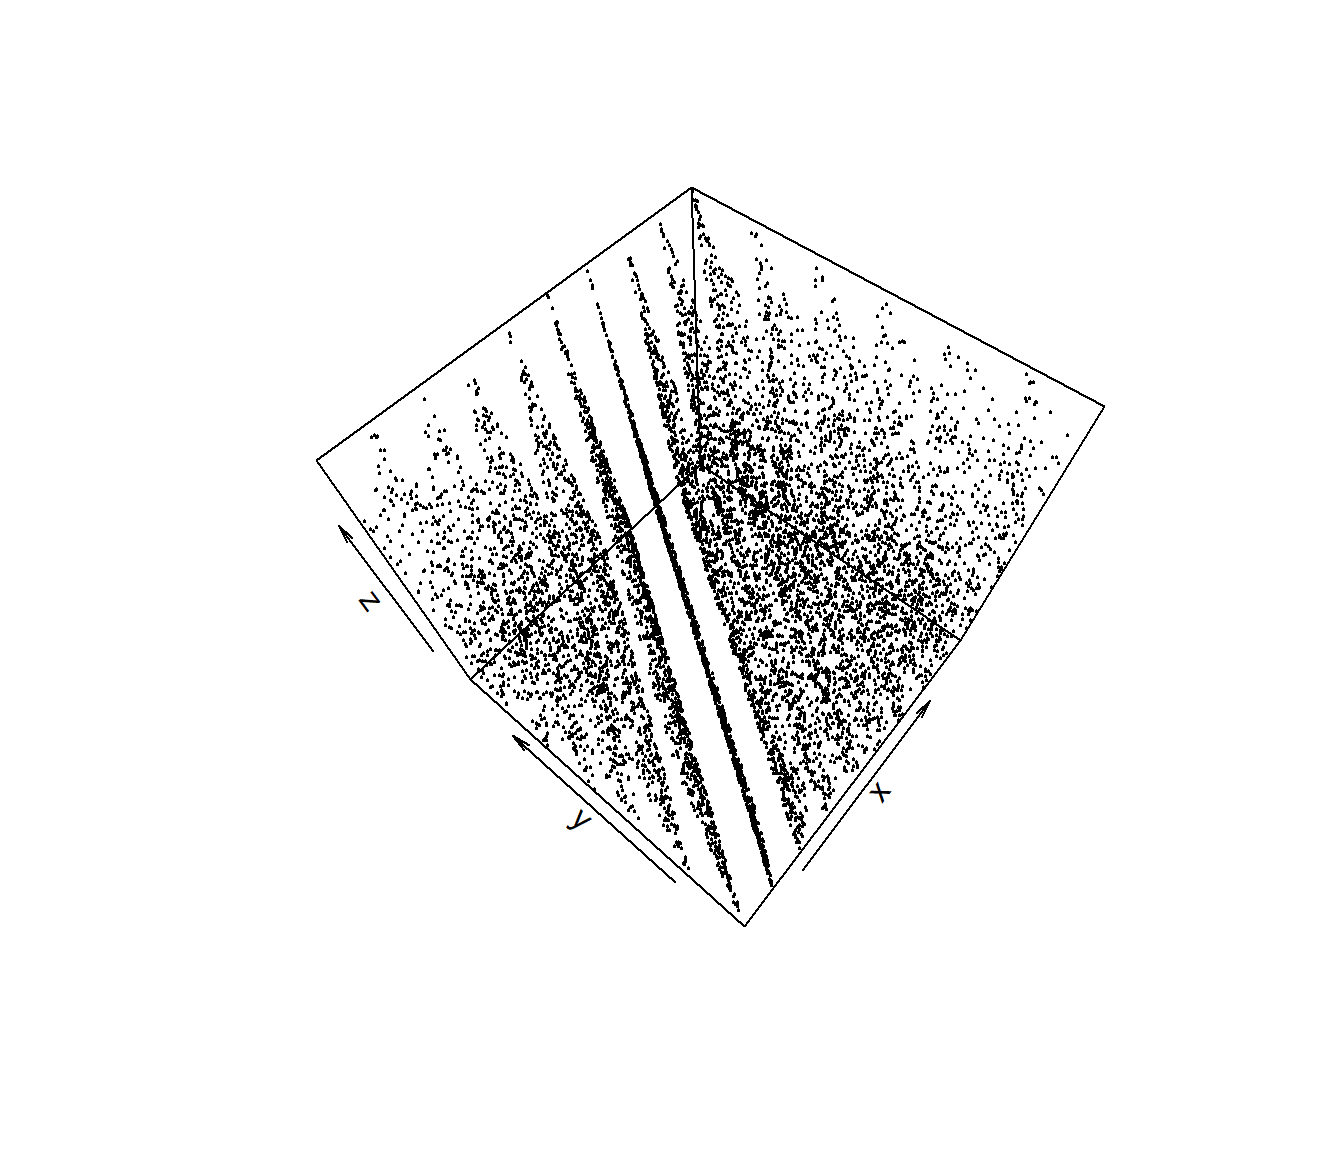
\includegraphics[width=0.7\linewidth]{03-Generacion_numeros_aleatorios_files/figure-latex/randu-1} 

}

\caption{Grafico de dispersión de tripletas del generador RANDU de IBM (contenidas en 15 planos)}\label{fig:randu}
\end{figure}

En general todos los generadores de este tipo van a presentar estructuras reticulares.
Marsaglia (1968) demostró que las \(k\)-uplas de un generadores multiplicativo están contenidas en a lo sumo \(\left(k!m\right)^{1/k}\) hiperplanos paralelos (para más detalles sobre la estructura reticular, ver por ejemplo Ripley, 1987, sección 2.7).
Por tanto habría que seleccionar adecuadamente \(m\) y \(c\) (\(a\) solo influiría en la pendiente) de forma que la estructura reticular sea impreceptible teniendo en cuenta el número de datos que se pretende generar (por ejemplo de forma que la distancia mínima entre los puntos sea próxima a la esperada en teoría).

Se han propuesto diversas pruebas (ver Sección \ref{calgen}) para
determinar si un generador tiene problemas de este tipo y se han
realizado numerosos estudios para determinadas familias (e.g.~Park y
Miller, 1988, estudiaron que parámetros son adecuados para \(m=2^{31}-1\)).

\begin{itemize}
\item
  En cualquier caso, se recomienda considerar un ``periodo de
  seguridad'' \(\approx \sqrt{p}\) para evitar este tipo de problemas.
\item
  Aunque estos generadores tiene limitaciones en su capacidad para
  producir secuencias muy largas de números i.i.d. \(\mathcal{U}(0,1)\),
  es un elemento básico en generadores más avanzados.
\end{itemize}

\hypertarget{otros-generadores}{%
\subsection{Otros generadores}\label{otros-generadores}}

Se han considerado diversas extensiones del generador congruencial lineal simple:

\begin{itemize}
\item
  Lineal múltiple:
  \(x_{i}= a_0 + a_1 x_{i-1} + a_2 x_{i-2} + \cdots + a_{k} x_{i-k} \bmod m\),
  con periodo \(p\leq m^{k}-1\).
\item
  No lineal:
  \(x_{i} = f\left( x_{i-1}, x_{i-2}, \cdots, x_{i-k} \right) \bmod m\).
  Por ejemplo \(x_{i} = a_0 + a_1 x_{i-1} + a_2 x_{i-1}^2 \bmod m\).
\item
  Matricial:
  \(\boldsymbol{x}_{i} = A_0 + A_1\boldsymbol{x}_{i-1} + A_2\boldsymbol{x}_{i-2} + \cdots + A_{k}\boldsymbol{x}_{i-k} \bmod m\).
\end{itemize}

Un ejemplo de generador congruencia lineal múltiple es el denominado \emph{generador de Fibonacci retardado} (Fibonacci-lagged generator; Knuth, 1969):
\[x_n = (x_{n-37} + x_{n-100}) \bmod 2^{30},\]
con un período aproximado de \(2^{129}\) y que puede ser empleado en R (lo cual no sería en principio recomendable; ver \href{https://www-cs-faculty.stanford.edu/~knuth/news02.html\#rng}{Knuth Recent News 2002}) estableciendo \texttt{kind} a \texttt{"Knuth-TAOCP-2002"} o \texttt{"Knuth-TAOCP"} en la llamada a \texttt{set.seed()} o \texttt{RNGkind()}.

El generador \emph{Mersenne-Twister} (Matsumoto y Nishimura, 1998), empleado por defecto en R, de periodo \(2^{19937}-1\) y equidistribution en 623 dimensiones, se puede expresar como un generador congruencial matricial lineal.

Un caso particular del generador lineal múltiple son los denominados \emph{generadores de registros desfasados} (más relacionados con la Criptografía).
Se generan bits de forma secuencial considerando \(m=2\) y \(a_{i} \in \left \{ 0,1\right \}\) y se van combinando \(l\) bits para obtener valores en el intervalo \((0, 1)\), por ejemplo \(u_i = 0 . x_{it+1} x_{it+2} \ldots x_{it+l}\), siendo \(t\) un parámetro denominado \emph{aniquilación} (Tausworthe, 1965).
Los cálculos se pueden realizar rápidamente mediante operaciones lógicas (los sumandos de la combinación lineal se traducen en un ``o'' exclusivo XOR), empleando directamente los registros del procesador (ver por ejemplo, Ripley, 1987, Algoritmo 2.1).

Otras alternativas consisten en la combinanción de varios generadores, las más empleadas son:

\begin{itemize}
\item
  Combinar las salidas: por ejemplo \(u_{i}=\sum_{l=1}^L u_{i}^{(l)} \bmod 1\), donde \(u_{i}^{(l)}\) es el \(i\)-ésimo valor obtenido con el generador \(l\).
\item
  Barajar las salidas: por ejemplo se crea una tabla empleando un generador y se utiliza otro para seleccionar el índice del valor que se va a devolver y posteriormente actualizar.
\end{itemize}

El generador \emph{L'Ecuyer-CMRG} (L'Ecuyer, 1999), empleado como base para la generación de múltiples secuencias en el paquete \texttt{parallel}, combina dos generadores concruenciales lineales múltiples de orden \(k=3\) (el periodo aproximado es \(2^{191}\)).

\begin{exercise}[Análisis de un generador congruencial]
\protect\hypertarget{exr:congru512}{}{\label{exr:congru512} \iffalse (Análisis de un generador congruencial) \fi{} }
\end{exercise}

Considera el generador congruencial definido por:
\[\begin{aligned}
x_{n+1}  & =(5x_{n}+1)\ \bmod\ 512,\nonumber\\
u_{n+1}  & =\frac{x_{n+1}}{512},\ n=0,1,\dots\nonumber
\end{aligned}\]
(de ciclo máximo).

NOTA: El algoritmo está implementado en el fichero \emph{RANDC.R} y se muestra en la Sección \ref{gen-cong}.

\begin{enumerate}
\def\labelenumi{\alph{enumi})}
\item
  Generar 500 valores de este generador, obtener el tiempo de CPU,
  representar su distribución mediante un histograma (en escala
  de densidades) y compararla con la densidad teórica.

\begin{Shaded}
\begin{Highlighting}[]
\KeywordTok{initRANDC}\NormalTok{(}\DecValTok{321}\NormalTok{, }\DecValTok{5}\NormalTok{, }\DecValTok{1}\NormalTok{, }\DecValTok{512}\NormalTok{)       }\CommentTok{# Establecer semilla y parámetros}
\NormalTok{nsim <-}\StringTok{ }\DecValTok{500}
\KeywordTok{system.time}\NormalTok{(u <-}\StringTok{ }\KeywordTok{RANDCN}\NormalTok{(nsim))  }\CommentTok{# Generar}
\end{Highlighting}
\end{Shaded}

\begin{verbatim}
##    user  system elapsed 
##       0       0       0
\end{verbatim}

\begin{Shaded}
\begin{Highlighting}[]
\KeywordTok{hist}\NormalTok{(u, }\DataTypeTok{freq =} \OtherTok{FALSE}\NormalTok{)}
\KeywordTok{abline}\NormalTok{(}\DataTypeTok{h =} \DecValTok{1}\NormalTok{)                   }\CommentTok{# Densidad uniforme}
\end{Highlighting}
\end{Shaded}

  \begin{figure}[!htb]

  {\centering 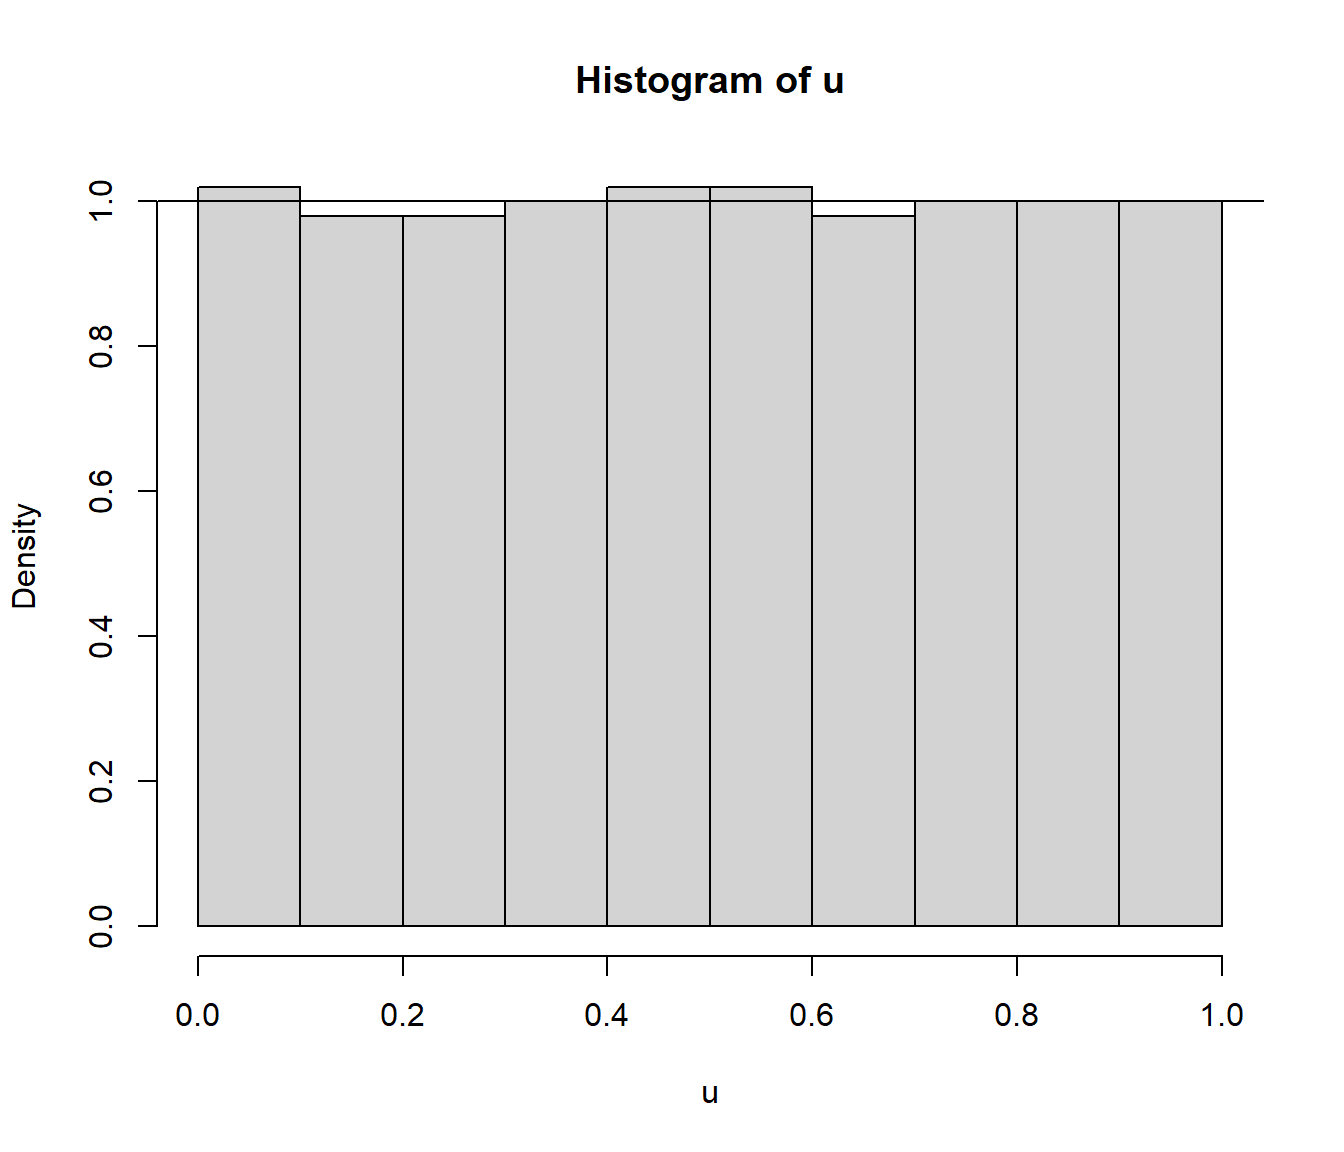
\includegraphics[width=0.7\linewidth]{03-Generacion_numeros_aleatorios_files/figure-latex/ejcona-1} 

  }

  \caption{Histograma de los valores generados}\label{fig:ejcona}
  \end{figure}

  En este caso concreto la distribución de los valores generados es aparentemente más uniforme de lo que cabría esperar, lo que induciría a sospechar de la calidad de este generador.
\item
  Calcular la media de las simulaciones (\texttt{mean}) y compararla con
  la teórica.

  La aproximación por simulación de la media teórica es:

\begin{Shaded}
\begin{Highlighting}[]
\KeywordTok{mean}\NormalTok{(u)}
\end{Highlighting}
\end{Shaded}

\begin{verbatim}
## [1] 0.4999609
\end{verbatim}

  La media teórica es 0.5.
  Error absoluto \(\ensuremath{3.90625\times 10^{-5}}\).
\item
  Aproximar (mediante simulación) la probabilidad del intervalo
  \((0.4;0.8)\) y compararla con la teórica.

  La probabilidad teórica es 0.8 - 0.4 = 0.4

  La aproximación mediante simulación:

\begin{Shaded}
\begin{Highlighting}[]
\KeywordTok{sum}\NormalTok{((}\FloatTok{0.4} \OperatorTok{<}\StringTok{ }\NormalTok{u) }\OperatorTok{&}\StringTok{ }\NormalTok{(u }\OperatorTok{<}\StringTok{ }\FloatTok{0.8}\NormalTok{))}\OperatorTok{/}\NormalTok{nsim}
\end{Highlighting}
\end{Shaded}

\begin{verbatim}
## [1] 0.402
\end{verbatim}

\begin{Shaded}
\begin{Highlighting}[]
\KeywordTok{mean}\NormalTok{((}\FloatTok{0.4} \OperatorTok{<}\StringTok{ }\NormalTok{u) }\OperatorTok{&}\StringTok{ }\NormalTok{(u }\OperatorTok{<}\StringTok{ }\FloatTok{0.8}\NormalTok{))     }\CommentTok{# Alternativa}
\end{Highlighting}
\end{Shaded}

\begin{verbatim}
## [1] 0.402
\end{verbatim}
\end{enumerate}

\hypertarget{calgen}{%
\section{Análisis de la calidad de un generador}\label{calgen}}

Para verificar si un generador tiene las propiedades estadísticas deseadas hay disponibles una gran cantidad de test de hipótesis y métodos gráficos,
incluyendo métodos genéricos (de bondad de ajuste y aleatoriedad) y contrastes específicos para generadores aleatorios.
Se trata principalmente de contrastar si las muestras generadas son i.i.d. \(\mathcal{U}\left(0,1\right)\) (análisis univariante).
Aunque los métodos más avanzados tratan normalmente de contrastar si las \(d\)-uplas:

\[(U_{t+1},U_{t+2},\ldots,U_{t+d}); \ t=(i-1)d, \ i=1,\ldots,m\]

son i.i.d. \(\mathcal{U}\left(0,1\right)^{d}\) (uniformes independientes en el hipercubo; análisis multivariante).
En el Apéndice \ref{gof-aleat} se describen algunos de estos métodos.

En esta sección emplearemos únicamente métodos genéricos, ya que también pueden ser de utilidad para evaluar generadores de variables no uniformes y para la construcción de modelos del sistema real (e.g.~para modelar variables que se tratarán como entradas del modelo general).
Sin embargo, los métodos clásicos pueden no ser muy adecuados para evaluar generadores de números pseudoaleatorios (e.g.~L'Ecuyer y Simard, 2007).
La recomendación sería emplear baterías de contrastes recientes, como las descritas en la Subsección \ref{baterias}.

Hay que destacar algunas diferencias entre el uso de este tipo de métodos en inferencia y en simulación.
Por ejemplo, si empleamos un constrate de hipótesis del modo habitual, desconfiamos del generador si la muestra (secuencia) no se ajusta a la distribución teórica (\(p\)-valor \(\leq \alpha\)).
En este caso además, también se sospecha si se ajusta demasiado
bien a la distribución teórica (\(p\)-valor \(\geq1-\alpha\)),
lo que indicaría que no reproduce adecuadamente la variabilidad.

Uno de los contrastes más conocidos es el test ji-cuadrado de bondad de ajuste
(\texttt{chisq.test} para el caso discreto).
Aunque si la variable de interés es continua, habría que discretizarla
(con la correspondiente perdida de información).
Por ejemplo, se podría emplear la siguiente función
(que imita a las incluídas en \texttt{R}):

\begin{Shaded}
\begin{Highlighting}[]
\CommentTok{#-------------------------------------------------------------------------------}
\CommentTok{# chisq.test.cont(x, distribution, nclasses, output, nestpar,...)}
\CommentTok{#-----------------------------------------------------------------------}
\CommentTok{# Realiza el test ji-cuadrado de bondad de ajuste para una distribución }
\CommentTok{# continua discretizando en intervalos equiprobables.}
\CommentTok{# Parámetros:}
\CommentTok{#   distribution = "norm","unif", etc}
\CommentTok{#   nclasses = floor(length(x)/5)}
\CommentTok{#   output = TRUE}
\CommentTok{#   nestpar = 0 = número de parámetros estimados}
\CommentTok{#   ... = parámetros distribución}
\CommentTok{# Ejemplo:}
\CommentTok{#   chisq.test.cont(x, distribution = "norm", nestpar = 2, }
\CommentTok{#                   mean = mean(x), sd = sqrt((nx - 1) / nx) * sd(x))}
\CommentTok{#-----------------------------------------------------------------------}
\NormalTok{chisq.test.cont <-}\StringTok{ }\ControlFlowTok{function}\NormalTok{(x, }\DataTypeTok{distribution =} \StringTok{"norm"}\NormalTok{, }
    \DataTypeTok{nclasses =} \KeywordTok{floor}\NormalTok{(}\KeywordTok{length}\NormalTok{(x)}\OperatorTok{/}\DecValTok{5}\NormalTok{), }\DataTypeTok{output =} \OtherTok{TRUE}\NormalTok{, }\DataTypeTok{nestpar =} \DecValTok{0}\NormalTok{, ...) \{}
    \CommentTok{# Funciones distribución}
\NormalTok{    q.distrib <-}\StringTok{ }\KeywordTok{eval}\NormalTok{(}\KeywordTok{parse}\NormalTok{(}\DataTypeTok{text =} \KeywordTok{paste}\NormalTok{(}\StringTok{"q"}\NormalTok{, distribution, }\DataTypeTok{sep =} \StringTok{""}\NormalTok{)))}
\NormalTok{    d.distrib <-}\StringTok{ }\KeywordTok{eval}\NormalTok{(}\KeywordTok{parse}\NormalTok{(}\DataTypeTok{text =} \KeywordTok{paste}\NormalTok{(}\StringTok{"d"}\NormalTok{, distribution, }\DataTypeTok{sep =} \StringTok{""}\NormalTok{)))}
    \CommentTok{# Puntos de corte}
\NormalTok{    q <-}\StringTok{ }\KeywordTok{q.distrib}\NormalTok{((}\DecValTok{1}\OperatorTok{:}\NormalTok{(nclasses }\OperatorTok{-}\StringTok{ }\DecValTok{1}\NormalTok{))}\OperatorTok{/}\NormalTok{nclasses, ...)}
\NormalTok{    tol <-}\StringTok{ }\KeywordTok{sqrt}\NormalTok{(.Machine}\OperatorTok{$}\NormalTok{double.eps)}
\NormalTok{    xbreaks <-}\StringTok{ }\KeywordTok{c}\NormalTok{(}\KeywordTok{min}\NormalTok{(x) }\OperatorTok{-}\StringTok{ }\NormalTok{tol, q, }\KeywordTok{max}\NormalTok{(x) }\OperatorTok{+}\StringTok{ }\NormalTok{tol)}
    \CommentTok{# Gráficos y frecuencias}
    \ControlFlowTok{if}\NormalTok{ (output) \{}
\NormalTok{        xhist <-}\StringTok{ }\KeywordTok{hist}\NormalTok{(x, }\DataTypeTok{breaks =}\NormalTok{ xbreaks, }\DataTypeTok{freq =} \OtherTok{FALSE}\NormalTok{, }
                      \DataTypeTok{lty =} \DecValTok{2}\NormalTok{, }\DataTypeTok{border =} \StringTok{"grey50"}\NormalTok{)}
        \KeywordTok{curve}\NormalTok{(}\KeywordTok{d.distrib}\NormalTok{(x, ...), }\DataTypeTok{add =} \OtherTok{TRUE}\NormalTok{)}
\NormalTok{    \} }\ControlFlowTok{else}\NormalTok{ \{}
\NormalTok{        xhist <-}\StringTok{ }\KeywordTok{hist}\NormalTok{(x, }\DataTypeTok{breaks =}\NormalTok{ xbreaks, }\DataTypeTok{plot =} \OtherTok{FALSE}\NormalTok{)}
\NormalTok{    \}}
    \CommentTok{# Cálculo estadístico y p-valor}
\NormalTok{    O <-}\StringTok{ }\NormalTok{xhist}\OperatorTok{$}\NormalTok{counts  }\CommentTok{# Equivalente a table(cut(x, xbreaks)) pero más eficiente}
\NormalTok{    E <-}\StringTok{ }\KeywordTok{length}\NormalTok{(x)}\OperatorTok{/}\NormalTok{nclasses}
\NormalTok{    DNAME <-}\StringTok{ }\KeywordTok{deparse}\NormalTok{(}\KeywordTok{substitute}\NormalTok{(x))}
\NormalTok{    METHOD <-}\StringTok{ "Pearson's Chi-squared test"}
\NormalTok{    STATISTIC <-}\StringTok{ }\KeywordTok{sum}\NormalTok{((O }\OperatorTok{-}\StringTok{ }\NormalTok{E)}\OperatorTok{^}\DecValTok{2}\OperatorTok{/}\NormalTok{E)}
    \KeywordTok{names}\NormalTok{(STATISTIC) <-}\StringTok{ "X-squared"}
\NormalTok{    PARAMETER <-}\StringTok{ }\NormalTok{nclasses }\OperatorTok{-}\StringTok{ }\NormalTok{nestpar }\OperatorTok{-}\StringTok{ }\DecValTok{1}
    \KeywordTok{names}\NormalTok{(PARAMETER) <-}\StringTok{ "df"}
\NormalTok{    PVAL <-}\StringTok{ }\KeywordTok{pchisq}\NormalTok{(STATISTIC, PARAMETER, }\DataTypeTok{lower.tail =} \OtherTok{FALSE}\NormalTok{)}
    \CommentTok{# Preparar resultados}
\NormalTok{    classes <-}\StringTok{ }\KeywordTok{format}\NormalTok{(xbreaks)}
\NormalTok{    classes <-}\StringTok{ }\KeywordTok{paste}\NormalTok{(}\StringTok{"("}\NormalTok{, classes[}\OperatorTok{-}\NormalTok{(nclasses }\OperatorTok{+}\StringTok{ }\DecValTok{1}\NormalTok{)], }\StringTok{","}\NormalTok{, classes[}\OperatorTok{-}\DecValTok{1}\NormalTok{], }\StringTok{"]"}\NormalTok{, }
        \DataTypeTok{sep =} \StringTok{""}\NormalTok{)}
\NormalTok{    RESULTS <-}\StringTok{ }\KeywordTok{list}\NormalTok{(}\DataTypeTok{classes =}\NormalTok{ classes, }\DataTypeTok{observed =}\NormalTok{ O, }\DataTypeTok{expected =}\NormalTok{ E, }\DataTypeTok{residuals =}\NormalTok{ (O }\OperatorTok{-}\StringTok{ }
\StringTok{        }\NormalTok{E)}\OperatorTok{/}\KeywordTok{sqrt}\NormalTok{(E))}
    \ControlFlowTok{if}\NormalTok{ (output) \{}
        \KeywordTok{cat}\NormalTok{(}\StringTok{"}\CharTok{\textbackslash{}n}\StringTok{Pearson's Chi-squared test table}\CharTok{\textbackslash{}n}\StringTok{"}\NormalTok{)}
        \KeywordTok{print}\NormalTok{(}\KeywordTok{as.data.frame}\NormalTok{(RESULTS))}
\NormalTok{    \}}
    \ControlFlowTok{if}\NormalTok{ (}\KeywordTok{any}\NormalTok{(E }\OperatorTok{<}\StringTok{ }\DecValTok{5}\NormalTok{)) }
        \KeywordTok{warning}\NormalTok{(}\StringTok{"Chi-squared approximation may be incorrect"}\NormalTok{)}
    \KeywordTok{structure}\NormalTok{(}\KeywordTok{c}\NormalTok{(}\KeywordTok{list}\NormalTok{(}\DataTypeTok{statistic =}\NormalTok{ STATISTIC, }\DataTypeTok{parameter =}\NormalTok{ PARAMETER, }\DataTypeTok{p.value =}\NormalTok{ PVAL, }
        \DataTypeTok{method =}\NormalTok{ METHOD, }\DataTypeTok{data.name =}\NormalTok{ DNAME), RESULTS), }\DataTypeTok{class =} \StringTok{"htest"}\NormalTok{)}
\NormalTok{\}}
\end{Highlighting}
\end{Shaded}

Continuando con el generador congruencial anterior, obtendríamos:

\begin{Shaded}
\begin{Highlighting}[]
\KeywordTok{chisq.test.cont}\NormalTok{(u, }\DataTypeTok{distribution =} \StringTok{"unif"}\NormalTok{, }
                \DataTypeTok{nclasses =} \DecValTok{10}\NormalTok{, }\DataTypeTok{nestpar =} \DecValTok{0}\NormalTok{, }\DataTypeTok{min =} \DecValTok{0}\NormalTok{, }\DataTypeTok{max =} \DecValTok{1}\NormalTok{)}
\end{Highlighting}
\end{Shaded}

\begin{figure}[!htb]

{\centering 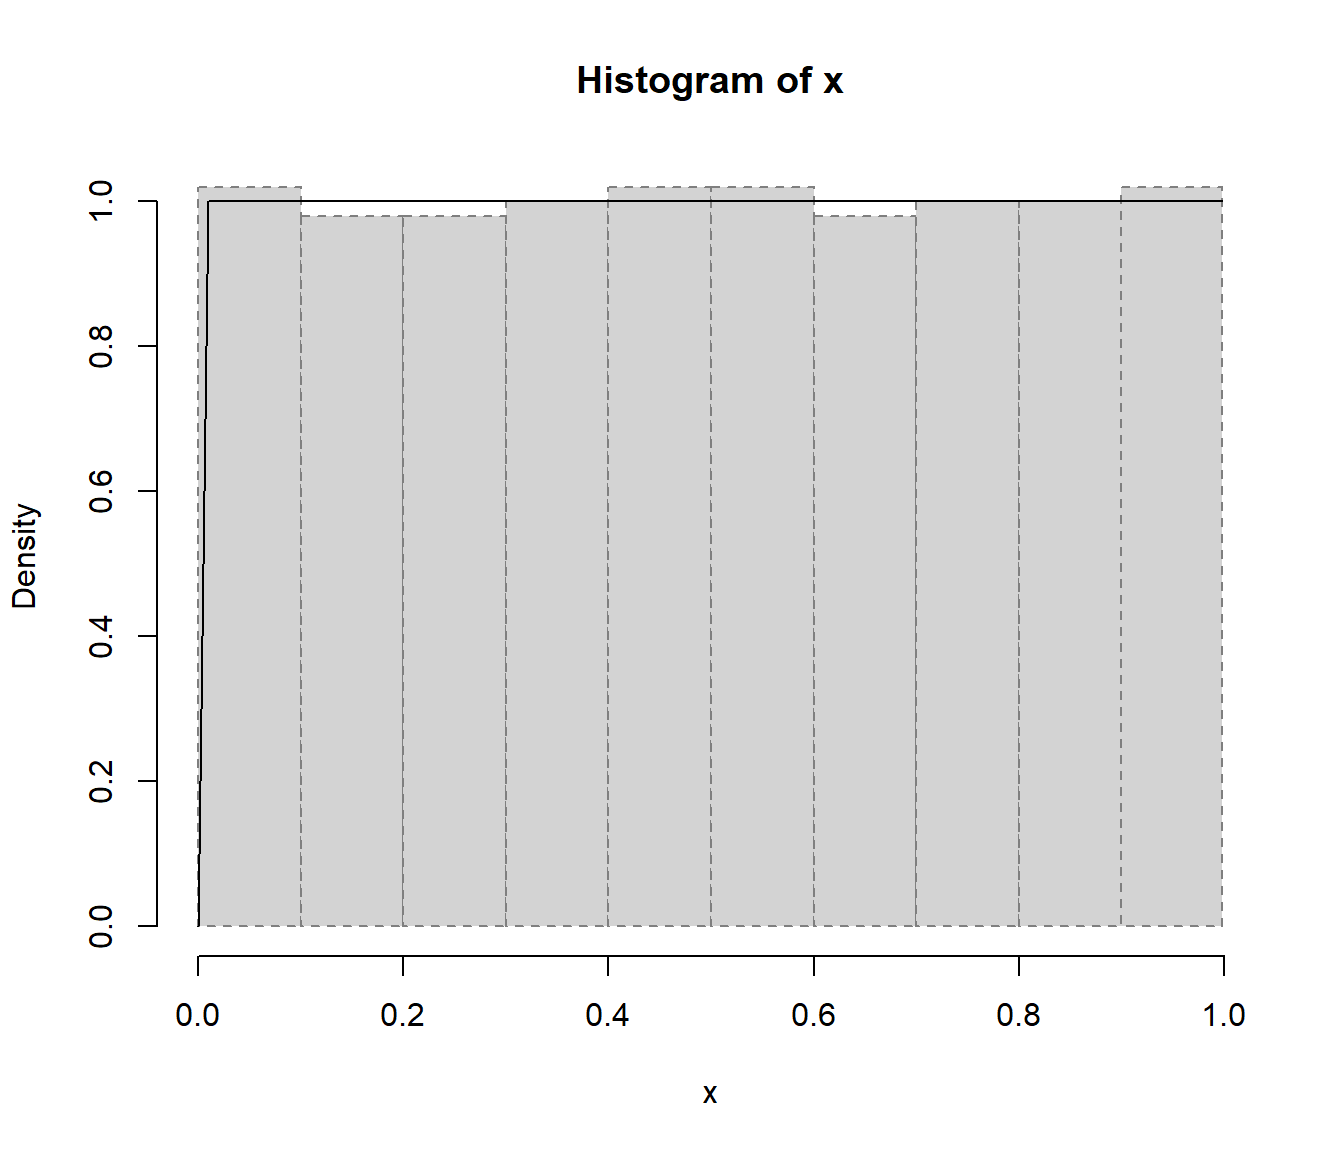
\includegraphics[width=0.7\linewidth]{03-Generacion_numeros_aleatorios_files/figure-latex/chisq-test-unif-1} 

}

\caption{Gráfico resultante de aplicar la función `chisq.test.cont()` comparando el histograma de los valores generados con la densidad uniforme.}\label{fig:chisq-test-unif}
\end{figure}

\begin{verbatim}
## 
## Pearson's Chi-squared test table
##                          classes observed expected  residuals
## 1  (-1.490116e-08, 1.000000e-01]       51       50  0.1414214
## 2  ( 1.000000e-01, 2.000000e-01]       49       50 -0.1414214
## 3  ( 2.000000e-01, 3.000000e-01]       49       50 -0.1414214
## 4  ( 3.000000e-01, 4.000000e-01]       50       50  0.0000000
## 5  ( 4.000000e-01, 5.000000e-01]       51       50  0.1414214
## 6  ( 5.000000e-01, 6.000000e-01]       51       50  0.1414214
## 7  ( 6.000000e-01, 7.000000e-01]       49       50 -0.1414214
## 8  ( 7.000000e-01, 8.000000e-01]       50       50  0.0000000
## 9  ( 8.000000e-01, 9.000000e-01]       50       50  0.0000000
## 10 ( 9.000000e-01, 9.980469e-01]       50       50  0.0000000
\end{verbatim}

\begin{verbatim}
## 
##  Pearson's Chi-squared test
## 
## data:  u
## X-squared = 0.12, df = 9, p-value = 1
\end{verbatim}

Como se muestra en la Figura \ref{fig:chisq-test-unif} el histograma de la secuencia generada es muy plano (comparado con lo que cabría esperar de una muestra de tamaño 500 de una uniforme), y consecuentemente el \(p\)-valor del contraste ji-cuadrado es prácticamente 1, lo que indicaría que este generador no reproduce adecuadamente la variabilidad de una distribución uniforme.

Otro contraste de bondad de ajuste muy conocido es el test de Kolmogorov-Smirnov, implementado en \texttt{ks.test} (ver Sección \ref{ks-test}).
En la Sección \ref{gof} se describen con más detalle estos contrastes.

\begin{exercise}[Análisis de un generador congruencial, continuación]
\protect\hypertarget{exr:congru512b}{}{\label{exr:congru512b} \iffalse (Análisis de un generador congruencial, continuación) \fi{} }
\end{exercise}

Continuando con el generador congruencial del Ejercicio \ref{exr:congru512}:

\begin{Shaded}
\begin{Highlighting}[]
\KeywordTok{initRANDC}\NormalTok{(}\DecValTok{321}\NormalTok{, }\DecValTok{5}\NormalTok{, }\DecValTok{1}\NormalTok{, }\DecValTok{512}\NormalTok{)}
\NormalTok{nsim <-}\StringTok{ }\DecValTok{500}
\KeywordTok{system.time}\NormalTok{(u <-}\StringTok{ }\KeywordTok{RANDCN}\NormalTok{(nsim))}
\end{Highlighting}
\end{Shaded}

\begin{enumerate}
\def\labelenumi{\alph{enumi})}
\item
  Realizar el contraste de Kolmogorov-Smirnov para estudiar el
  ajuste a una \(\mathcal{U}(0,1)\).

  Este contraste de hipótesis compara la función de distribución bajo la hipótesis nula con la función de distribución empírica (ver Sección \ref{empdistr}), representadas en la Figura \ref{fig:empdistrunif}:

\begin{Shaded}
\begin{Highlighting}[]
\CommentTok{# Distribución empírica}
\KeywordTok{curve}\NormalTok{(}\KeywordTok{ecdf}\NormalTok{(u)(x), }\DataTypeTok{type =} \StringTok{"s"}\NormalTok{, }\DataTypeTok{lwd =} \DecValTok{2}\NormalTok{)}
\KeywordTok{curve}\NormalTok{(}\KeywordTok{punif}\NormalTok{(x, }\DecValTok{0}\NormalTok{, }\DecValTok{1}\NormalTok{), }\DataTypeTok{add =} \OtherTok{TRUE}\NormalTok{)}
\end{Highlighting}
\end{Shaded}

  \begin{figure}[!htb]

  {\centering 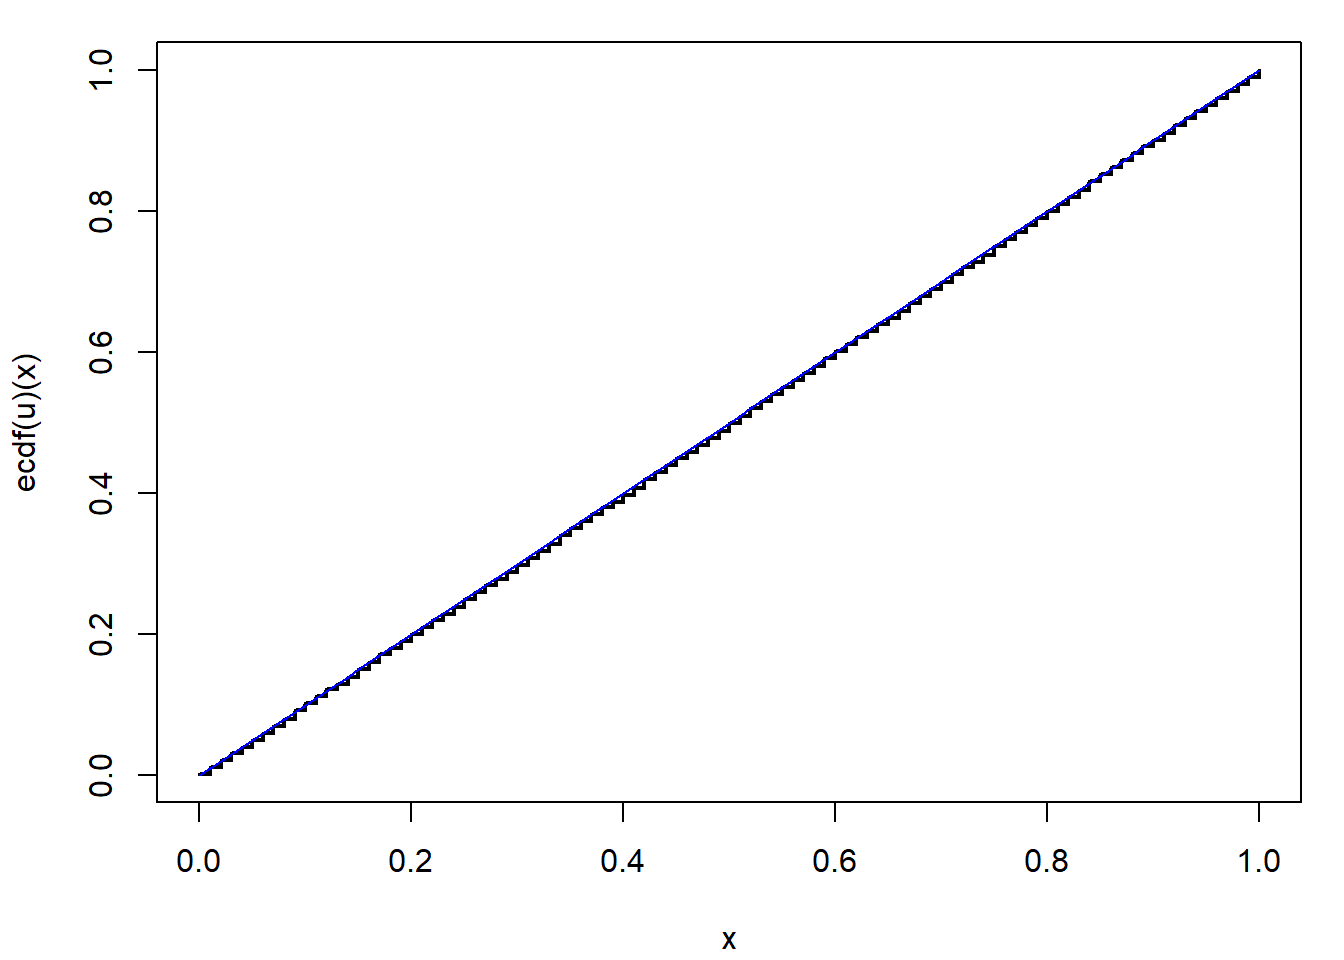
\includegraphics[width=0.7\linewidth]{03-Generacion_numeros_aleatorios_files/figure-latex/empdistrunif-1} 

  }

  \caption{Comparación de la distribución empírica de la secuencia generada con la función de distribución uniforme.}\label{fig:empdistrunif}
  \end{figure}

  Podemos realizar el contraste con el siguiente código:

\begin{Shaded}
\begin{Highlighting}[]
\CommentTok{# Test de Kolmogorov-Smirnov}
\KeywordTok{ks.test}\NormalTok{(u, }\StringTok{"punif"}\NormalTok{, }\DecValTok{0}\NormalTok{, }\DecValTok{1}\NormalTok{)}
\end{Highlighting}
\end{Shaded}

\begin{verbatim}
## 
##  One-sample Kolmogorov-Smirnov test
## 
## data:  u
## D = 0.0033281, p-value = 1
## alternative hypothesis: two-sided
\end{verbatim}
\item
  Obtener el gráfico secuencial y el de dispersión retardado, ¿se
  observa algún problema?

  Gráfico secuencial:

\begin{Shaded}
\begin{Highlighting}[]
\KeywordTok{plot}\NormalTok{(}\KeywordTok{as.ts}\NormalTok{(u))}
\end{Highlighting}
\end{Shaded}

  \begin{figure}[!htb]

  {\centering 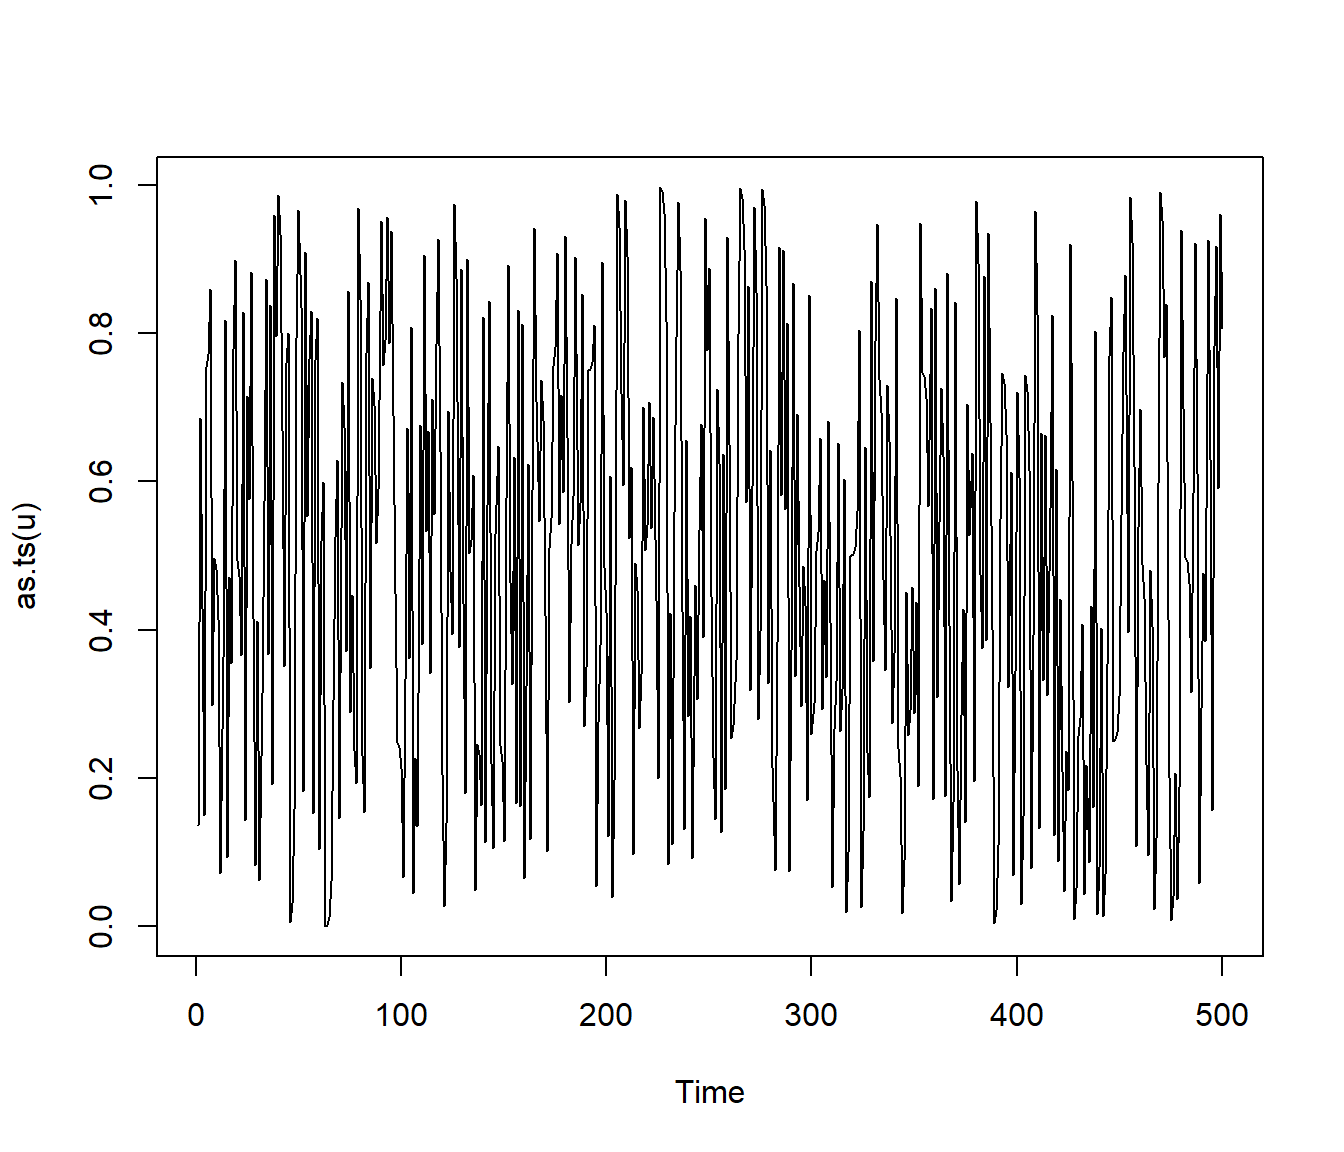
\includegraphics[width=0.7\linewidth]{03-Generacion_numeros_aleatorios_files/figure-latex/plot-sec-1} 

  }

  \caption{Gráfico secuencial de los valores generados.}\label{fig:plot-sec}
  \end{figure}

  Gráfico de dispersión retardado:

\begin{Shaded}
\begin{Highlighting}[]
\KeywordTok{plot}\NormalTok{(u[}\OperatorTok{-}\NormalTok{nsim],u[}\OperatorTok{-}\DecValTok{1}\NormalTok{])}
\end{Highlighting}
\end{Shaded}

  \begin{figure}[!htb]

  {\centering 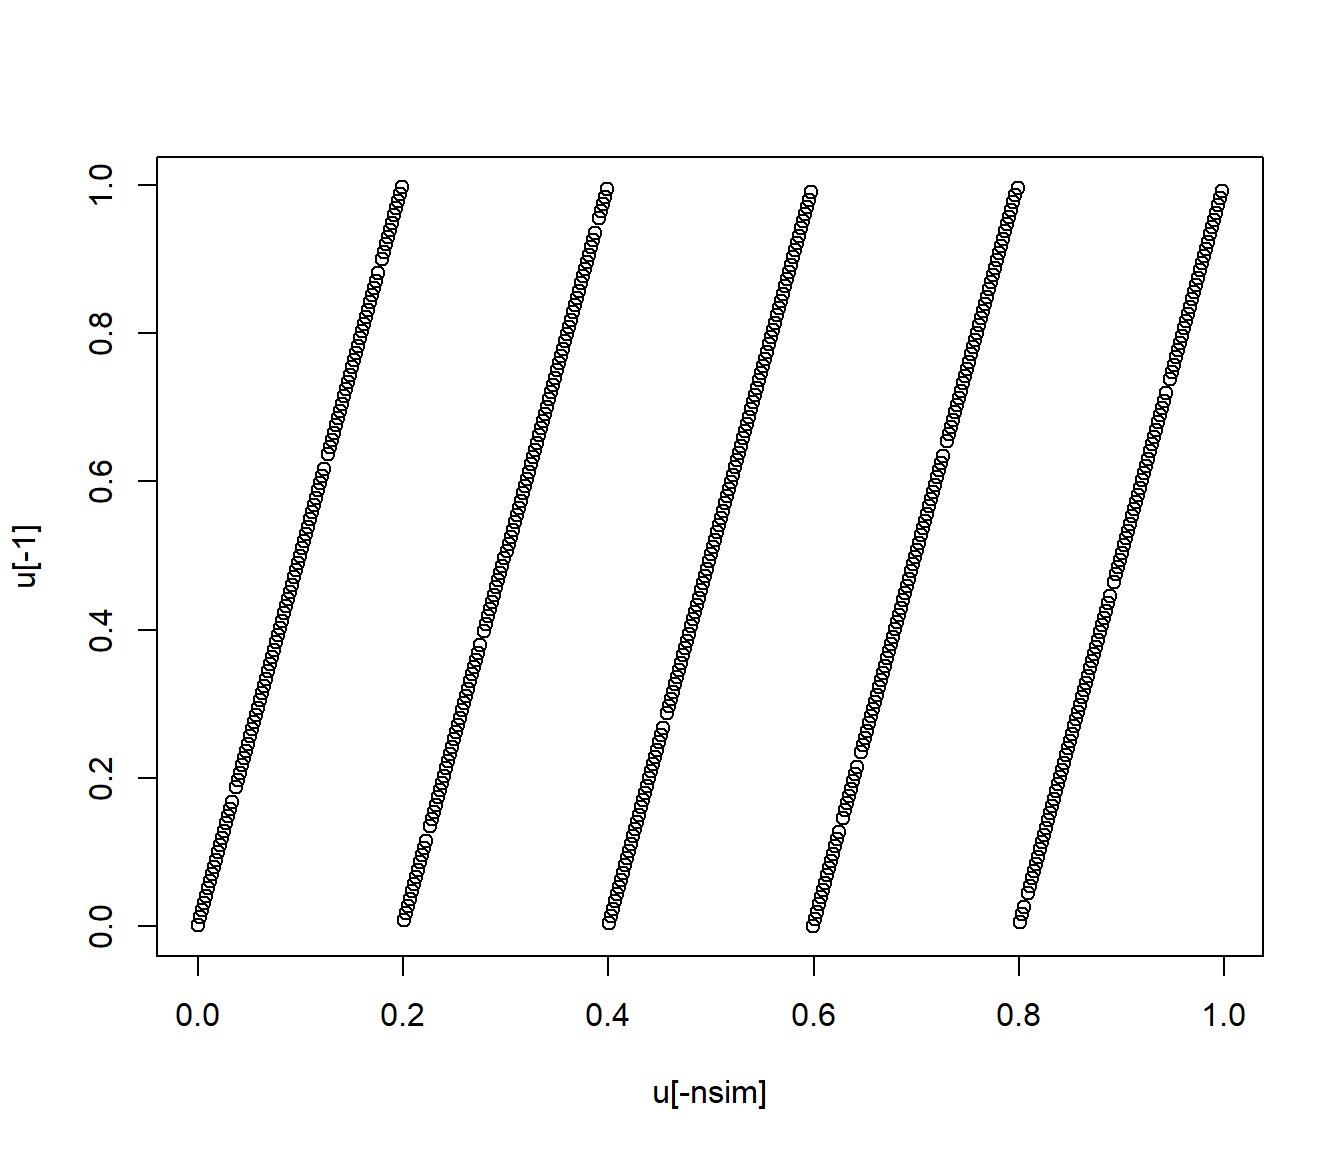
\includegraphics[width=0.7\linewidth]{03-Generacion_numeros_aleatorios_files/figure-latex/plot-ret-1} 

  }

  \caption{Gráfico de dispersión retardado de los valores generados.}\label{fig:plot-ret}
  \end{figure}
\item
  Estudiar las correlaciones del vector \((u_{i},u_{i+k})\), con
  \(k=1,\ldots,10\). Contrastar si son nulas.

  Correlaciones:

\begin{Shaded}
\begin{Highlighting}[]
\KeywordTok{acf}\NormalTok{(u)}
\end{Highlighting}
\end{Shaded}

  \begin{figure}[!htb]

  {\centering 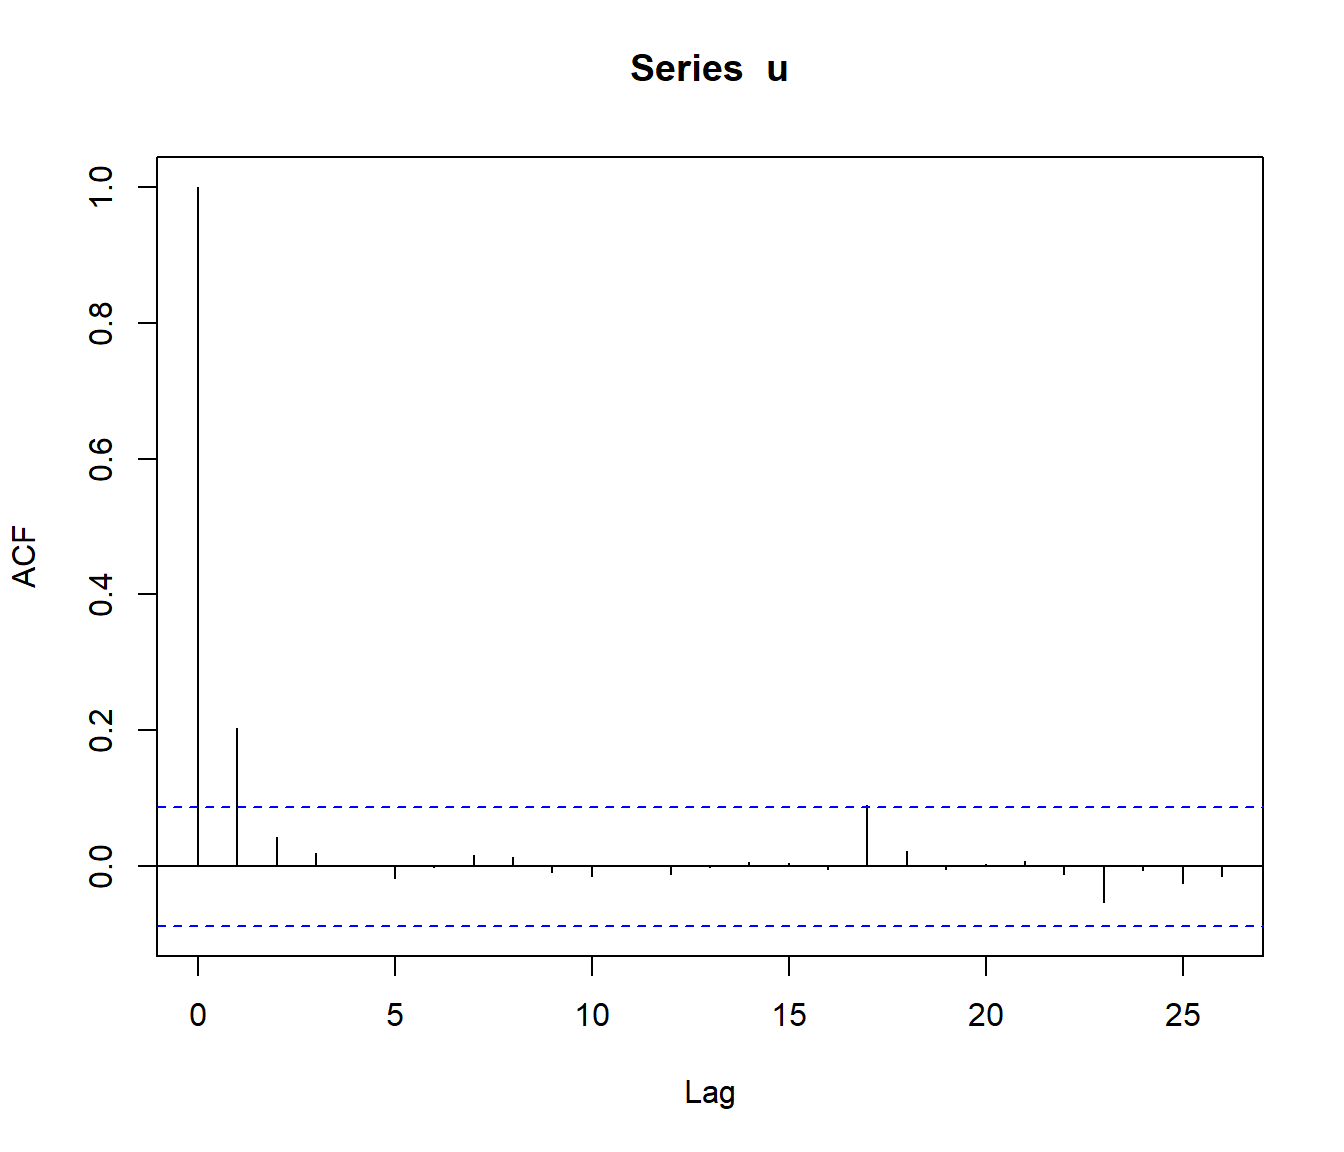
\includegraphics[width=0.7\linewidth]{03-Generacion_numeros_aleatorios_files/figure-latex/plot-acf-1} 

  }

  \caption{Autocorrelaciones de los valores generados.}\label{fig:plot-acf}
  \end{figure}

  Test de Ljung-Box:

\begin{Shaded}
\begin{Highlighting}[]
\KeywordTok{Box.test}\NormalTok{(u, }\DataTypeTok{lag =} \DecValTok{10}\NormalTok{, }\DataTypeTok{type =} \StringTok{"Ljung"}\NormalTok{)}
\end{Highlighting}
\end{Shaded}

\begin{verbatim}
## 
##  Box-Ljung test
## 
## data:  u
## X-squared = 22.533, df = 10, p-value = 0.01261
\end{verbatim}
\end{enumerate}

\hypertarget{repeticiuxf3n-de-contrastes}{%
\subsection{Repetición de contrastes}\label{repeticiuxf3n-de-contrastes}}

Los contrastes se plantean habitualmente desde el punto de vista de
la inferencia estadística en la práctica: se realiza una prueba
sobre la única muestra disponible. Si se realiza una única prueba,
en las condiciones de \(H_0\) hay
una probabilidad \(\alpha\) de rechazarla.
En simulación tiene mucho más sentido realizar un gran número de
pruebas:

\begin{itemize}
\item
  La proporción de rechazos debería aproximarse al valor de
  \(\alpha\)(se puede comprobar para distintos valores de \(\alpha\)).
\item
  La distribución del estadístico debería ajustarse a la teórica
  bajo \(H_0\)(se podría realizar un nuevo contraste de bondad
  de ajuste).
\item
  Los \emph{p}-valores obtenidos deberían ajustarse a una
  \(\mathcal{U}\left(0,1\right)\) (se podría realizar también un
  contraste de bondad de ajuste).
\end{itemize}

Este procedimiento es también el habitual para validar un método de
contraste de hipótesis por simulación.

\begin{example}
\protect\hypertarget{exm:rep-test-randu}{}{\label{exm:rep-test-randu} }
\end{example}

Consideramos el generador congruencial RANDU:

\begin{Shaded}
\begin{Highlighting}[]
\CommentTok{# Valores iniciales}
\KeywordTok{initRANDC}\NormalTok{(}\DecValTok{543210}\NormalTok{)   }\CommentTok{# Fijar semilla para reproductibilidad}
\CommentTok{# set.seed(543210)}
\NormalTok{n <-}\StringTok{ }\DecValTok{500}
\NormalTok{nsim <-}\StringTok{ }\DecValTok{1000}
\NormalTok{estadistico <-}\StringTok{ }\KeywordTok{numeric}\NormalTok{(nsim)}
\NormalTok{pvalor <-}\StringTok{ }\KeywordTok{numeric}\NormalTok{(nsim)}

\CommentTok{# Realizar contrastes}
\ControlFlowTok{for}\NormalTok{(isim }\ControlFlowTok{in} \DecValTok{1}\OperatorTok{:}\NormalTok{nsim) \{}
\NormalTok{  u <-}\StringTok{ }\KeywordTok{RANDCN}\NormalTok{(n)    }\CommentTok{# Generar}
  \CommentTok{# u <- runif(n)}
\NormalTok{  tmp <-}\StringTok{ }\KeywordTok{chisq.test.cont}\NormalTok{(u, }\DataTypeTok{distribution=}\StringTok{"unif"}\NormalTok{, }
            \DataTypeTok{nclasses=}\DecValTok{100}\NormalTok{, }\DataTypeTok{output=}\OtherTok{FALSE}\NormalTok{, }\DataTypeTok{nestpar=}\DecValTok{0}\NormalTok{, }\DataTypeTok{min=}\DecValTok{0}\NormalTok{, }\DataTypeTok{max=}\DecValTok{1}\NormalTok{)}
\NormalTok{  estadistico[isim] <-}\StringTok{ }\NormalTok{tmp}\OperatorTok{$}\NormalTok{statistic}
\NormalTok{  pvalor[isim] <-}\StringTok{ }\NormalTok{tmp}\OperatorTok{$}\NormalTok{p.value}
\NormalTok{\}}
\end{Highlighting}
\end{Shaded}

Proporción de rechazos:

\begin{Shaded}
\begin{Highlighting}[]
\CommentTok{# cat("\textbackslash{}nProporción de rechazos al 1% =", sum(pvalor < 0.01)/nsim, "\textbackslash{}n")}
\KeywordTok{cat}\NormalTok{(}\StringTok{"}\CharTok{\textbackslash{}n}\StringTok{Proporción de rechazos al 1% ="}\NormalTok{, }\KeywordTok{mean}\NormalTok{(pvalor }\OperatorTok{<}\StringTok{ }\FloatTok{0.01}\NormalTok{), }\StringTok{"}\CharTok{\textbackslash{}n}\StringTok{"}\NormalTok{)}
\end{Highlighting}
\end{Shaded}

\begin{verbatim}
## 
## Proporción de rechazos al 1% = 0.014
\end{verbatim}

\begin{Shaded}
\begin{Highlighting}[]
\CommentTok{# cat("Proporción de rechazos al 5% =", sum(pvalor < 0.05)/nsim, "\textbackslash{}n")}
\KeywordTok{cat}\NormalTok{(}\StringTok{"Proporción de rechazos al 5% ="}\NormalTok{, }\KeywordTok{mean}\NormalTok{(pvalor }\OperatorTok{<}\StringTok{ }\FloatTok{0.05}\NormalTok{), }\StringTok{"}\CharTok{\textbackslash{}n}\StringTok{"}\NormalTok{)}
\end{Highlighting}
\end{Shaded}

\begin{verbatim}
## Proporción de rechazos al 5% = 0.051
\end{verbatim}

\begin{Shaded}
\begin{Highlighting}[]
\CommentTok{# cat("Proporción de rechazos al 10% =", sum(pvalor < 0.1)/nsim, "\textbackslash{}n")}
\KeywordTok{cat}\NormalTok{(}\StringTok{"Proporción de rechazos al 10% ="}\NormalTok{, }\KeywordTok{mean}\NormalTok{(pvalor }\OperatorTok{<}\StringTok{ }\FloatTok{0.1}\NormalTok{), }\StringTok{"}\CharTok{\textbackslash{}n}\StringTok{"}\NormalTok{)}
\end{Highlighting}
\end{Shaded}

\begin{verbatim}
## Proporción de rechazos al 10% = 0.112
\end{verbatim}

Análisis del estadístico contraste:

\begin{Shaded}
\begin{Highlighting}[]
\CommentTok{# Histograma}
\KeywordTok{hist}\NormalTok{(estadistico, }\DataTypeTok{breaks =} \StringTok{"FD"}\NormalTok{, }\DataTypeTok{freq=}\OtherTok{FALSE}\NormalTok{)}
\KeywordTok{curve}\NormalTok{(}\KeywordTok{dchisq}\NormalTok{(x,}\DecValTok{99}\NormalTok{), }\DataTypeTok{add=}\OtherTok{TRUE}\NormalTok{)}
\end{Highlighting}
\end{Shaded}

\begin{center}\includegraphics[width=0.7\linewidth]{03-Generacion_numeros_aleatorios_files/figure-latex/unnamed-chunk-12-1} \end{center}

\begin{Shaded}
\begin{Highlighting}[]
\CommentTok{# Test ji-cuadrado}
\CommentTok{# chisq.test.cont(estadistico, distribution="chisq", nclasses=20, nestpar=0, df=99)}
\CommentTok{# Test de Kolmogorov-Smirnov}
\KeywordTok{ks.test}\NormalTok{(estadistico, }\StringTok{"pchisq"}\NormalTok{, }\DataTypeTok{df=}\DecValTok{99}\NormalTok{)}
\end{Highlighting}
\end{Shaded}

\begin{verbatim}
## 
##  One-sample Kolmogorov-Smirnov test
## 
## data:  estadistico
## D = 0.023499, p-value = 0.6388
## alternative hypothesis: two-sided
\end{verbatim}

Análisis de los \emph{p}-valores:

\begin{Shaded}
\begin{Highlighting}[]
\CommentTok{# Histograma}
\KeywordTok{hist}\NormalTok{(pvalor, }\DataTypeTok{freq=}\OtherTok{FALSE}\NormalTok{)}
\KeywordTok{abline}\NormalTok{(}\DataTypeTok{h=}\DecValTok{1}\NormalTok{) }\CommentTok{# curve(dunif(x,0,1), add=TRUE)}
\end{Highlighting}
\end{Shaded}

\begin{center}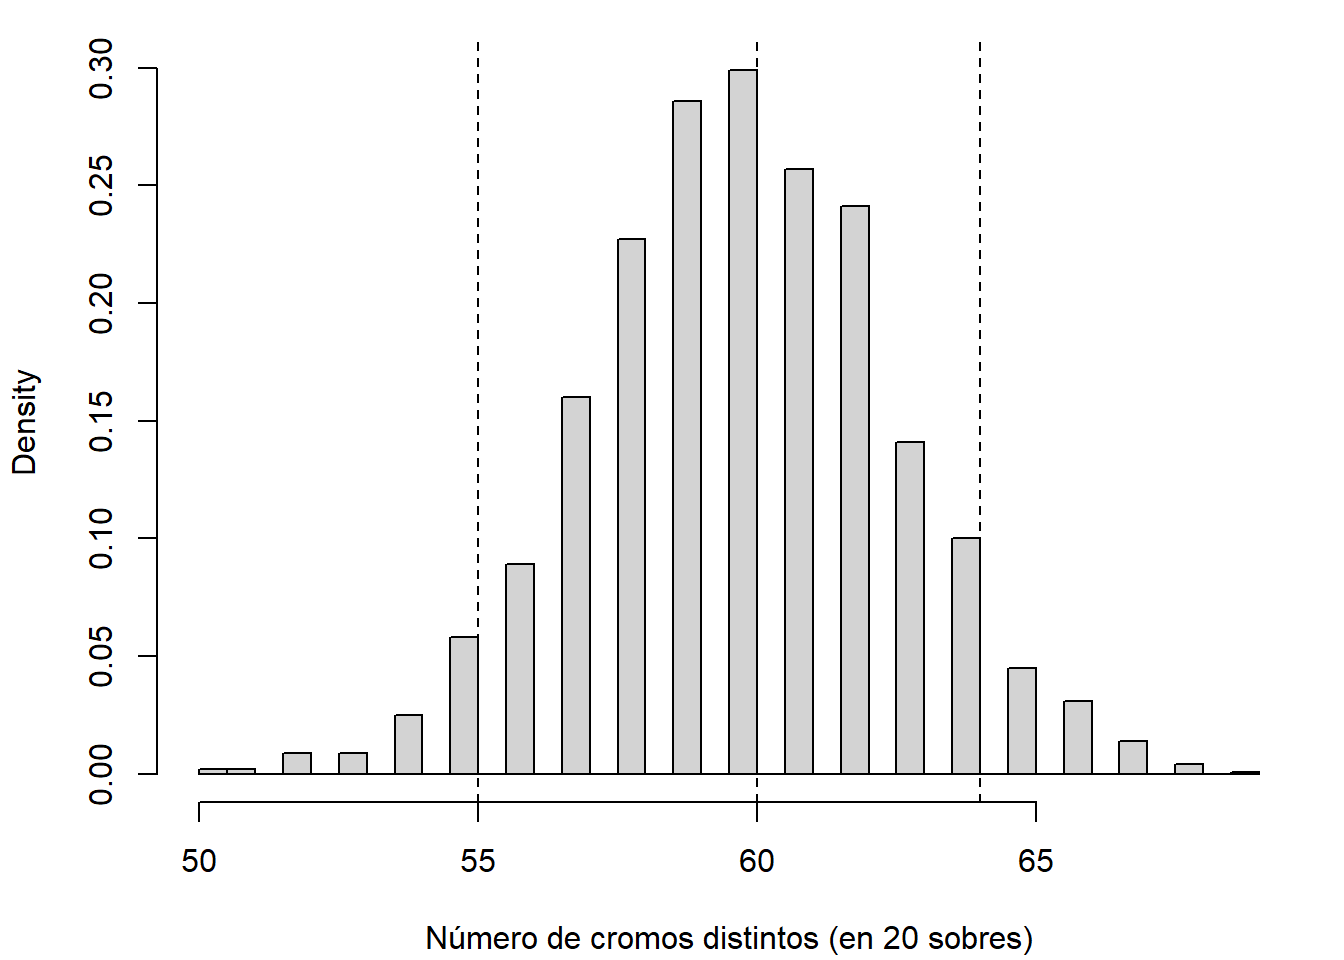
\includegraphics[width=0.7\linewidth]{03-Generacion_numeros_aleatorios_files/figure-latex/unnamed-chunk-13-1} \end{center}

\begin{Shaded}
\begin{Highlighting}[]
\CommentTok{# Test ji-cuadrado}
\CommentTok{# chisq.test.cont(pvalor, distribution="unif", nclasses=20, nestpar=0, min=0, max=1)}
\CommentTok{# Test de Kolmogorov-Smirnov}
\KeywordTok{ks.test}\NormalTok{(pvalor, }\StringTok{"punif"}\NormalTok{,  }\DataTypeTok{min=}\DecValTok{0}\NormalTok{, }\DataTypeTok{max=}\DecValTok{1}\NormalTok{)}
\end{Highlighting}
\end{Shaded}

\begin{verbatim}
## 
##  One-sample Kolmogorov-Smirnov test
## 
## data:  pvalor
## D = 0.023499, p-value = 0.6388
## alternative hypothesis: two-sided
\end{verbatim}

Adicionalmente, si queremos estudiar la proporción de rechazos (el \emph{tamaño del contraste}) para los posibles valores de \(\alpha\), podemos emplear la distribución empírica del \(p\)-valor (proporción de veces que resultó menor que un determinado valor):

\begin{Shaded}
\begin{Highlighting}[]
\CommentTok{# Distribución empírica}
\KeywordTok{curve}\NormalTok{(}\KeywordTok{ecdf}\NormalTok{(pvalor)(x), }\DataTypeTok{type =} \StringTok{"s"}\NormalTok{, }\DataTypeTok{lwd =} \DecValTok{2}\NormalTok{, }
      \DataTypeTok{xlab =} \StringTok{'Nivel de significación', ylab = '}\NormalTok{Proporción de rechazos}\StringTok{')}
\StringTok{abline(a = 0, b = 1, lty = 2)   # curve(punif(x, 0, 1), add = TRUE)}
\end{Highlighting}
\end{Shaded}

\begin{center}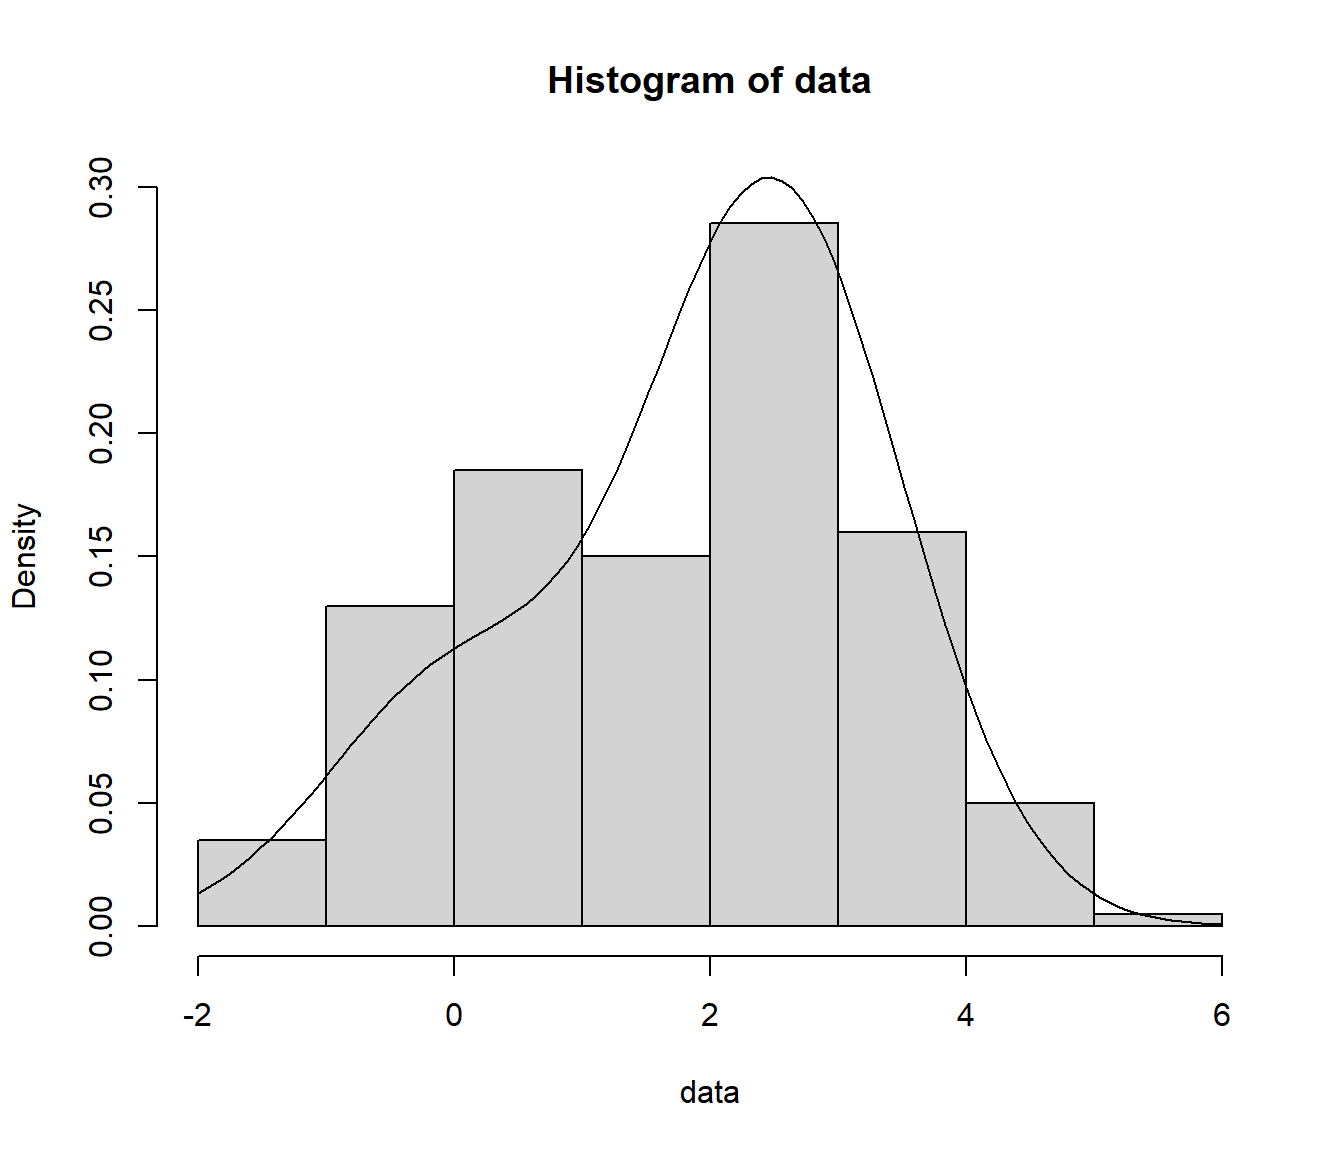
\includegraphics[width=0.7\linewidth]{03-Generacion_numeros_aleatorios_files/figure-latex/unnamed-chunk-14-1} \end{center}

\hypertarget{baterias}{%
\subsection{Baterías de contrastes}\label{baterias}}

Hay numerosos ejemplos de generadores que pasaron diferentes test de uniformidad y aleatoriedad pero que fallaron estrepitosamente al considerar nuevos contrastes diseñados específicamente para generadores aleatorios (ver Marsaglia \emph{et al.}, 1990).
Por este motivo, el procedimiento habitual en la práctica es aplicar un número más o menos elevado de contrastes (de distinto tipo y difíciles de pasar, e.g.~Marsaglia y Tsang, 2002), de forma que si el generador los pasa tendremos mayor confianza en que sus propiedades son las adecuadas.
Este conjunto de pruebas es lo que se denomina batería de contrastes. Una de las primeras se introdujo en Knuth (1969) y de las más recientes podríamos destacar:

\begin{itemize}
\item
  Diehard tests (The Marsaglia Random Number CDROM, 1995):
  \href{https://web.archive.org/web/20160125103112/http://stat.fsu.edu/pub/diehard}{http://www.stat.fsu.edu/pub/diehard (versión archivada el 2016-01-25)}.
\item
  Dieharder (Brown y Bauer, 2003):
  \href{https://webhome.phy.duke.edu/~rgb/General/dieharder.php}{Dieharder Page},
  paquete \href{https://github.com/eddelbuettel/rdieharder}{\texttt{RDieHarder}}.
\item
  TestU01 (L'Ecuyer y Simard, 2007):
  \url{http://simul.iro.umontreal.ca/testu01/tu01.html}.
\item
  NIST test suite (National Institute of Standards and Technology, USA, 2010):
  \url{http://csrc.nist.gov/groups/ST/toolkit/rng}.
\end{itemize}

Para más detalles, ver por ejemplo\footnote{También puede ser de interés el enlace \href{http://www.ciphersbyritter.com/RES/RANDTEST.HTM}{Randomness Tests: A Literature Survey} y la entidad certificadora (gratuita) en línea \href{http://www.cacert.at/random}{CAcert}.}:

\begin{itemize}
\item
  Marsaglia, G. y Tsang, W.W. (2002). \href{http://www.jstatsoft.org/v07/i03}{Some difficult-to-pass tests of randomness}. Journal of Statistical Software, 7(3), 1-9.
\item
  Demirhan, H. y Bitirim, N. (2016). \href{https://journal.r-project.org/archive/2016/RJ-2016-016/index.html}{CryptRndTest: an R package for testing the cryptographic randomness}.
  The R Journal, 8(1), 233-247.
\end{itemize}

\hypertarget{ejercicios-1}{%
\section{Ejercicios}\label{ejercicios-1}}

\begin{exercise}[Método de los cuadrados medios]
\protect\hypertarget{exr:RANDVN}{}{\label{exr:RANDVN} \iffalse (Método de los cuadrados medios) \fi{} }
\end{exercise}
Uno de los primeros generadores fue el denominado método de los
cuadrados medios propuesto por Von Neumann (1946). Con este
procedimiento se generan números pseudoaleatorios de 4 dígitos de la
siguiente forma:

\begin{enumerate}
\def\labelenumi{\roman{enumi}.}
\item
  Se escoge un número de cuatro dígitos \(x_0\) (semilla).
\item
  Se eleva al cuadrado (\(x_0^2\)) y se toman los cuatro dígitos centrales (\(x_1\)).
\item
  Se genera el número pseudo-aleatorio como \[u_1=\frac{x_1}{10^{4}}.\]
\item
  Volver al paso ii y repetir el proceso.
\end{enumerate}

Para obtener los \(k\) (número par) dígitos centrales de \(x_{i}^2\)
se puede utilizar que:
\[x_{i+1}=\left\lfloor \left(  x_{i}^2-\left\lfloor \dfrac{x_{i}^2}{10^{(2k-\frac{k}2)}}\right\rfloor 10^{(2k-\frac{k}2)}\right)
/10^{\frac{k}2}\right\rfloor\]

El algoritmo está implementado en el fichero \emph{RANDVN.R}:

\begin{Shaded}
\begin{Highlighting}[]
\CommentTok{# -------------------------------------------------}
\CommentTok{# Generador Von Neumann de números pseudoaleatorios}
\CommentTok{# -------------------------------------------------}

\CommentTok{# initRANDVN(semilla,n)}
\CommentTok{# -----------------------}
\CommentTok{#   Inicia el generador }
\CommentTok{#   n número de digitos centrales, 4 por defecto (debe ser un número par)}
\CommentTok{#   Por defecto semilla del reloj}
\CommentTok{#   OJO: No se hace ninguna verificación de los parámetros}
\NormalTok{initRANDVN <-}\StringTok{ }\ControlFlowTok{function}\NormalTok{(}\DataTypeTok{semilla =} \KeywordTok{as.numeric}\NormalTok{(}\KeywordTok{Sys.time}\NormalTok{()), }\DataTypeTok{n =} \DecValTok{4}\NormalTok{) \{}
\NormalTok{  .semilla <<-}\StringTok{ }\KeywordTok{as.double}\NormalTok{(semilla) }\OperatorTok\StringTok{ }\DecValTok{10}\OperatorTok{^}\NormalTok{n  }\CommentTok{# Cálculos en doble precisión}
\NormalTok{  .n <<-}\StringTok{ }\NormalTok{n}
\NormalTok{  .aux <<-}\StringTok{ }\DecValTok{10}\OperatorTok{^}\NormalTok{(}\DecValTok{2}\OperatorTok{*}\NormalTok{n}\OperatorTok{-}\NormalTok{n}\OperatorTok{/}\DecValTok{2}\NormalTok{)}
\NormalTok{  .aux2 <<-}\StringTok{ }\DecValTok{10}\OperatorTok{^}\NormalTok{(n}\OperatorTok{/}\DecValTok{2}\NormalTok{)}
  \KeywordTok{return}\NormalTok{(}\KeywordTok{invisible}\NormalTok{(}\KeywordTok{list}\NormalTok{(}\DataTypeTok{semilla=}\NormalTok{.semilla,}\DataTypeTok{n=}\NormalTok{.n)))}
\NormalTok{\}}

\CommentTok{# RANDVN()}
\CommentTok{# -----------------------}
\CommentTok{#   Genera un valor pseudoaleatorio con el generador de Von Neumann.}
\CommentTok{#   Actualiza la semilla (si no existe llama a initRANDVN).}
\NormalTok{RANDVN <-}\StringTok{ }\ControlFlowTok{function}\NormalTok{() \{}
    \ControlFlowTok{if}\NormalTok{ (}\OperatorTok{!}\KeywordTok{exists}\NormalTok{(}\StringTok{".semilla"}\NormalTok{, }\DataTypeTok{envir=}\KeywordTok{globalenv}\NormalTok{())) }\KeywordTok{initRANDVN}\NormalTok{()}
\NormalTok{    z <-}\StringTok{ }\NormalTok{.semilla}\OperatorTok{^}\DecValTok{2}
\NormalTok{    .semilla <<-}\StringTok{ }\KeywordTok{trunc}\NormalTok{((z}\OperatorTok{-}\KeywordTok{trunc}\NormalTok{(z}\OperatorTok{/}\NormalTok{.aux)}\OperatorTok{*}\NormalTok{.aux)}\OperatorTok{/}\NormalTok{.aux2)}
    \KeywordTok{return}\NormalTok{(.semilla}\OperatorTok{/}\DecValTok{10}\OperatorTok{^}\NormalTok{.n)}
\NormalTok{\}}

\CommentTok{# RANDVNN(n)}
\CommentTok{# -----------------------}
\CommentTok{#   Genera un vector de valores pseudoaleatorios, de dimensión `n` }
\CommentTok{#   con elgenerador de Von Neumann.}
\CommentTok{#   Actualiza la semilla (si no existe llama a initRANDVN).}
\NormalTok{RANDVNN <-}\StringTok{ }\ControlFlowTok{function}\NormalTok{(}\DataTypeTok{n =} \DecValTok{1000}\NormalTok{) \{}
\NormalTok{    x <-}\StringTok{ }\KeywordTok{numeric}\NormalTok{(n)}
    \ControlFlowTok{for}\NormalTok{(i }\ControlFlowTok{in} \DecValTok{1}\OperatorTok{:}\NormalTok{n) x[i] <-}\StringTok{ }\KeywordTok{RANDVN}\NormalTok{()}
    \KeywordTok{return}\NormalTok{(x)}
    \CommentTok{# return(replicate(n,RANDVN()))  # Alternativa más rápida}
\NormalTok{\}}
\end{Highlighting}
\end{Shaded}

Estudiar las características del
generador de cuadrados medios a partir de una secuencia de 500
valores. Emplear únicamente métodos gráficos.

\begin{exercise}
\protect\hypertarget{exr:parkmiller}{}{\label{exr:parkmiller} }
\end{exercise}
Considerando el generador congruencial multiplicativo de parámetros
\(a=7^{5}=16807\), \(c=0\) y \(m=2^{31}-1\). ¿Se observan los mismos problemas
que con el algoritmo RANDU al considerar las tripletas \((x_{k},x_{k+1},x_{k+2})\)?

\hypertarget{cap4}{%
\chapter{Análisis de resultados de simulación}\label{cap4}}

Work in progress\ldots{}

En este capítulo nos centraremos en la aproximación mediante simulación de la media teórica de un estadístico a partir de la media muestral de una secuencia de simulaciones de dicho estadístico.
La aproximación de una probabilidad sería un caso particular considerando una variable de Bernouilli.

En primer lugar se tratará el análisis de la convergencia y la precisión de la aproximación por simulación.
Al final del capítulo se incluye una breve introducción a los problemas de estabilización y dependencia (con los que nos solemos encontrar en simulación dinámica y MCMC).

\hypertarget{convergencia}{%
\section{Convergencia}\label{convergencia}}

Supongamos que estamos interesados en aproximar la media teórica
\(\mu = E\left( X\right)\) a partir de una secuencia i.i.d. \(X_{1}\),
\(X_{2}\), \(\cdots\), \(X_{n}\) mediante la media muestral \(\bar{X}_{n}\).
Una justificación teórica de la validez de la aproximación obtenida
mediante simulación es \emph{la ley (débil) de los grandes números}:

\begin{itemize}
\item
  Si \(X_{1}\), \(X_{2}\), \(\cdots\) es una secuencia de variables aleatorias
  independientes con:
  \[E\left( X_{i}\right) =\mu \text{ y }Var\left( X_{i}\right) 
  =\sigma^{2}<\infty,\]
  entonces \(\overline{X}_{n}=\left( X_{1}+\cdots +X_{n}\right) /n\)
  converge en probabilidad a \(\mu\). i.e.~para cualquier \(\varepsilon >0\):
  \[\lim\limits_{n\rightarrow \infty }P\left( \left\vert \overline{X}_{n}-\mu
  \right\vert <\varepsilon \right) = 1.\]
\item
  \emph{La ley fuerte} establece la convergencia casi segura.
\end{itemize}

\begin{example}
\protect\hypertarget{exm:unnamed-chunk-2}{}{\label{exm:unnamed-chunk-2} }Aproximación de una probabilidad
\end{example}
Simulamos una distribución de Bernoulli de parámetro \(p=0.5\):

\begin{Shaded}
\begin{Highlighting}[]
\NormalTok{p <-}\StringTok{ }\FloatTok{0.5}
\KeywordTok{set.seed}\NormalTok{(}\DecValTok{1}\NormalTok{)}
\NormalTok{nsim <-}\StringTok{ }\DecValTok{10000}
\CommentTok{# nsim <- 100}
\NormalTok{rx <-}\StringTok{ }\KeywordTok{runif}\NormalTok{(nsim) }\OperatorTok{<=}\StringTok{ }\NormalTok{p}
\end{Highlighting}
\end{Shaded}

La aproximación por simulación de \(p\) será:

\begin{Shaded}
\begin{Highlighting}[]
\KeywordTok{mean}\NormalTok{(rx) }
\end{Highlighting}
\end{Shaded}

\begin{verbatim}
## [1] 0.5047
\end{verbatim}

Podemos generar un gráfico con la evolución de la aproximación con el siguiente código:

\begin{Shaded}
\begin{Highlighting}[]
\KeywordTok{plot}\NormalTok{(}\KeywordTok{cumsum}\NormalTok{(rx)}\OperatorTok{/}\DecValTok{1}\OperatorTok{:}\NormalTok{nsim, }\DataTypeTok{type=}\StringTok{"l"}\NormalTok{, }\DataTypeTok{lwd=}\DecValTok{2}\NormalTok{, }\DataTypeTok{xlab=}\StringTok{"Número de generaciones"}\NormalTok{, }
     \DataTypeTok{ylab=}\StringTok{"Proporción muestral"}\NormalTok{, }\DataTypeTok{ylim=}\KeywordTok{c}\NormalTok{(}\DecValTok{0}\NormalTok{,}\DecValTok{1}\NormalTok{))}
\KeywordTok{abline}\NormalTok{(}\DataTypeTok{h =} \KeywordTok{mean}\NormalTok{(rx), }\DataTypeTok{lty =} \DecValTok{2}\NormalTok{)}
\CommentTok{# valor teórico}
\KeywordTok{abline}\NormalTok{(}\DataTypeTok{h =}\NormalTok{ p) }
\end{Highlighting}
\end{Shaded}

\begin{figure}[!htb]

{\centering 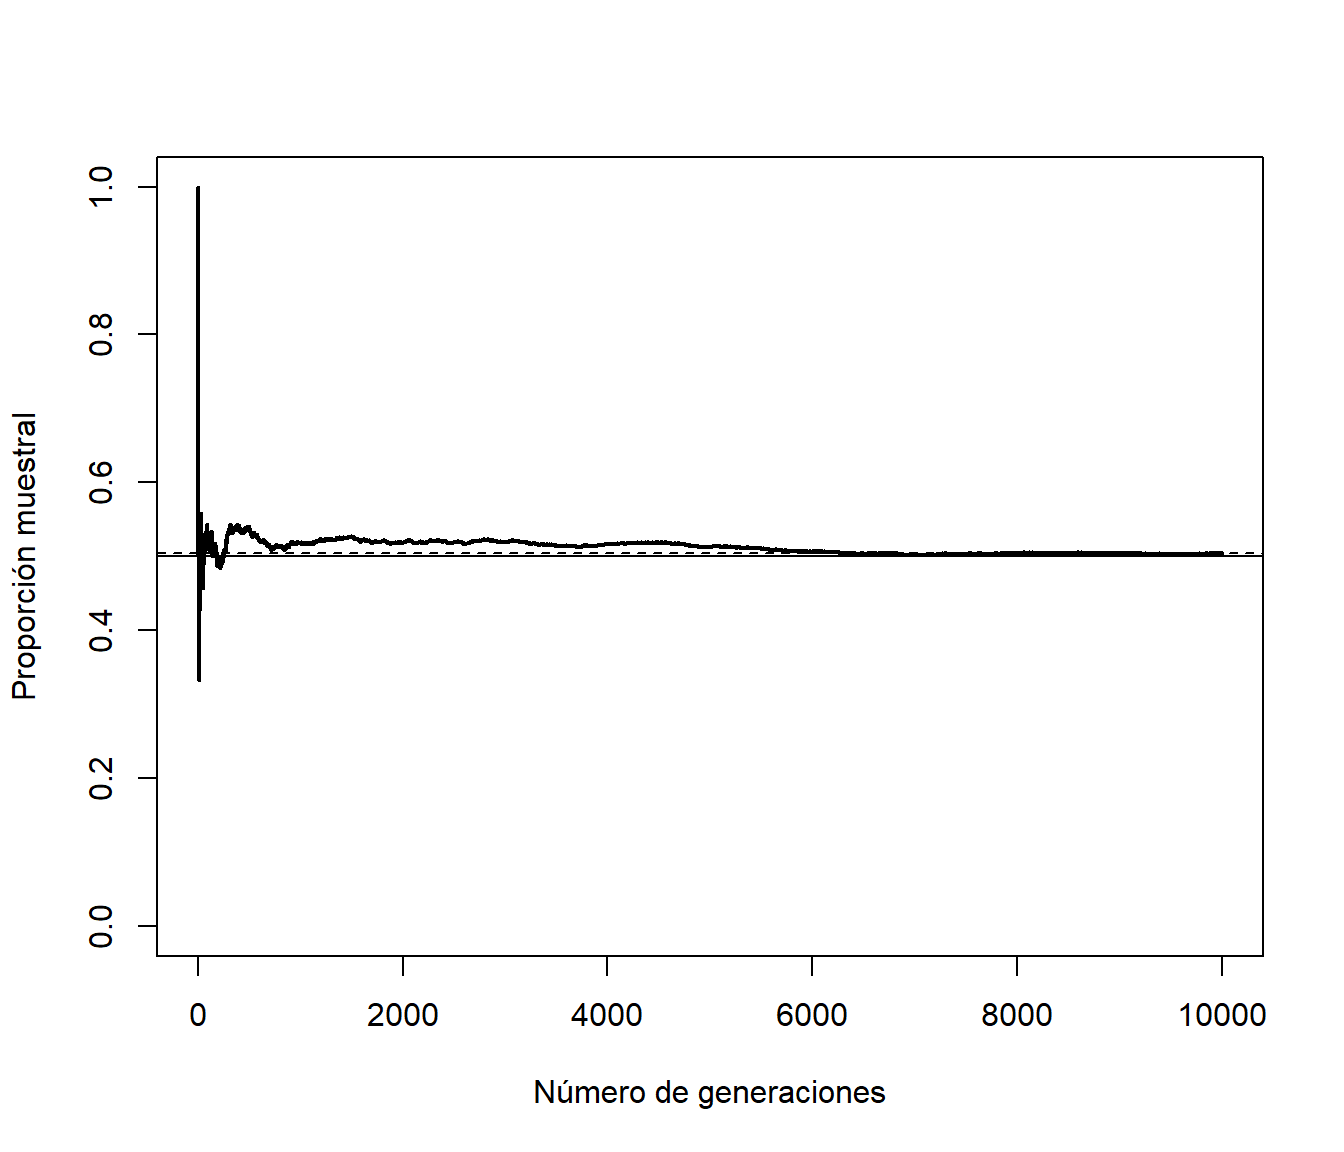
\includegraphics[width=0.7\linewidth]{04-Analisis_resultados_files/figure-latex/proporcion-1} 

}

\caption{Aproximación de la proporción en función del número de generaciones.}\label{fig:proporcion}
\end{figure}

\hypertarget{detecciuxf3n-de-problemas-de-convergencia}{%
\subsection{Detección de problemas de convergencia}\label{detecciuxf3n-de-problemas-de-convergencia}}

Una suposición crucial es que las variables \(X_{i}\) deben tener
varianza finita (realmente esta suposición puede relajarse:
\(E\left( \left\vert X_{i} \right\vert \right) < \infty\)).
En caso contrario la media muestral puede no converger a
una constante. Un ejemplo conocido es la distribución de Cauchy:

\begin{Shaded}
\begin{Highlighting}[]
\KeywordTok{set.seed}\NormalTok{(}\DecValTok{1}\NormalTok{)}
\NormalTok{nsim <-}\StringTok{ }\DecValTok{10000}
\NormalTok{rx <-}\StringTok{ }\KeywordTok{rcauchy}\NormalTok{(nsim)}
\KeywordTok{plot}\NormalTok{(}\KeywordTok{cumsum}\NormalTok{(rx)}\OperatorTok{/}\DecValTok{1}\OperatorTok{:}\NormalTok{nsim, }\DataTypeTok{type=}\StringTok{"l"}\NormalTok{, }\DataTypeTok{lwd=}\DecValTok{2}\NormalTok{, }
     \DataTypeTok{xlab=}\StringTok{"Número de generaciones"}\NormalTok{, }\DataTypeTok{ylab=}\StringTok{"Media muestral"}\NormalTok{)}
\end{Highlighting}
\end{Shaded}

\begin{figure}[!htb]

{\centering 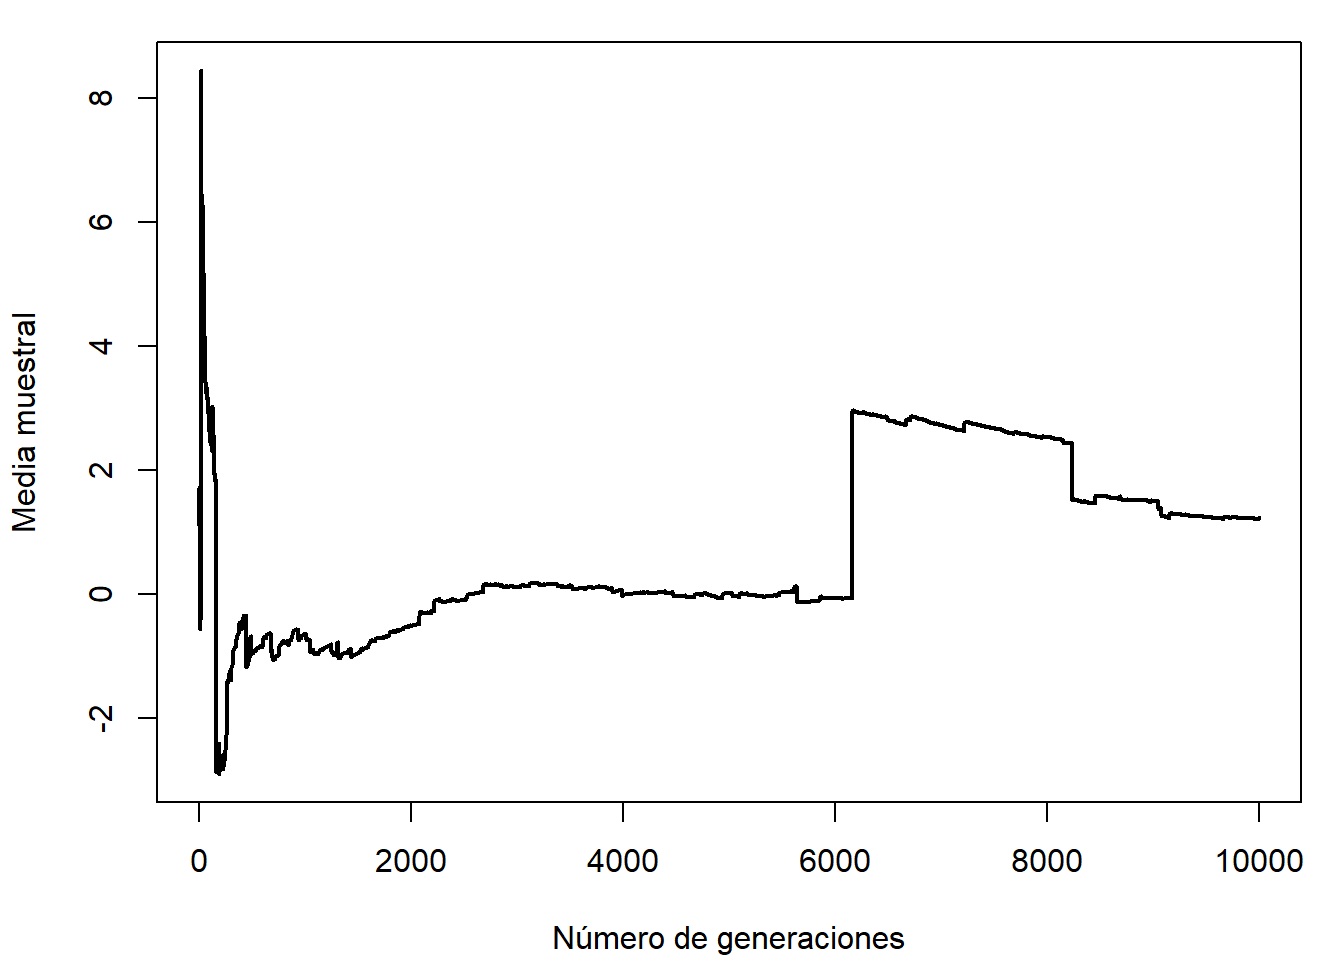
\includegraphics[width=0.7\linewidth]{04-Analisis_resultados_files/figure-latex/cauchy-1} 

}

\caption{Evolución de la media muestral de una distribución de Cauchy en función del número de generaciones.}\label{fig:cauchy}
\end{figure}

Para detectar problemas de convergencia es recomendable representar la evolución de la aproximación de la característica de interés (sobre el número de generaciones),
además de realizar otros análisis descriptivos de las simulaciones.
Por ejemplo, en este caso podemos observar los valores que producen estos saltos mediante un gráfico de cajas:

\begin{Shaded}
\begin{Highlighting}[]
\KeywordTok{boxplot}\NormalTok{(rx)}
\end{Highlighting}
\end{Shaded}

\begin{figure}[!htb]

{\centering 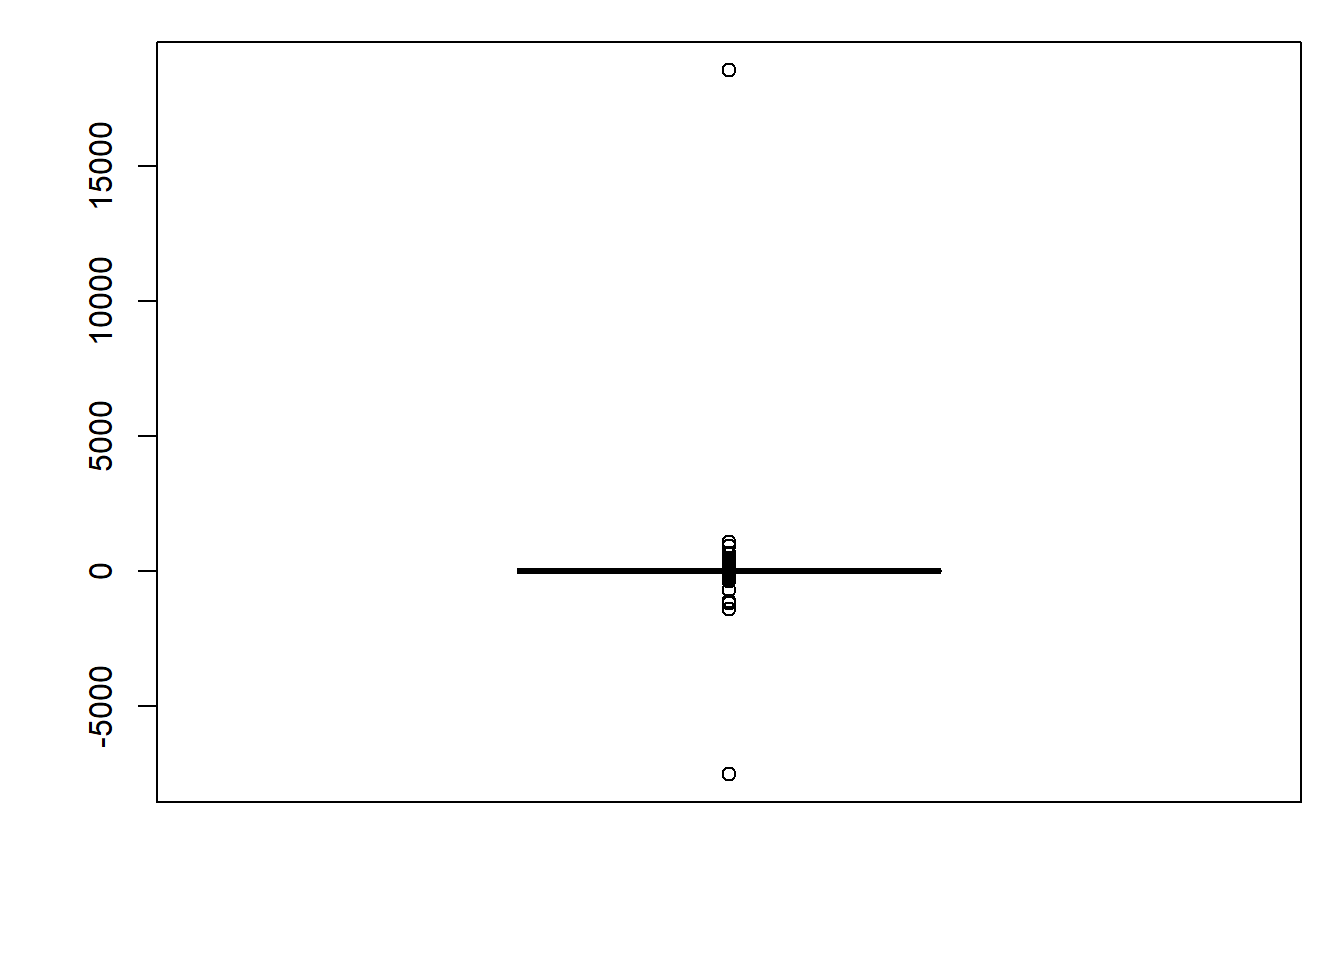
\includegraphics[width=0.7\linewidth]{04-Analisis_resultados_files/figure-latex/cauchy-box-1} 

}

\caption{Gráfico de cajas de 10000 generaciones de una distribución de Cauchy.}\label{fig:cauchy-box}
\end{figure}

\hypertarget{estimaciuxf3n-de-la-precisiuxf3n}{%
\section{Estimación de la precisión}\label{estimaciuxf3n-de-la-precisiuxf3n}}

En el caso de la media muestral \(\overline{X}_{n}\), un estimador
insesgado de \(Var\left( \overline{X}_{n}\right) =\sigma ^{2}/n\) es la cuasi-varianza muestral:
\[\widehat{Var}\left( \overline{X}_{n}\right) =\frac{\widehat{S}^{2}}{n}\]
con:
\[\widehat{S}_{n}^{2}=\dfrac{1}{n-1}\sum\limits_{i=1}^{n}\left( X_{i}-
\overline{X}\right) ^{2}.\]

En el caso de una proporción \(\hat{p}_{n}\):
\[\widehat{Var}\left( \hat{p}_{n}\right) 
=\frac{\hat{p}_{n}(1-\hat{p}_{n})}{n-1},\]
aunque se suele emplear la varianza muestral.

Los valores obtenidos servirían como medidas básicas de la precisión
de la aproximación, aunque su principal aplicación es la
construcción de intervalos de confianza.

\hypertarget{teorema-central-del-luxedmite}{%
\section{Teorema central del límite}\label{teorema-central-del-luxedmite}}

Si \(X_{1}\), \(X_{2}\), \(\cdots\) es una secuencia de variables aleatorias
independientes con \(E\left( X_{i}\right) =\mu\) y
\(Var\left( X_{i}\right) = \sigma ^{2}<\infty\), entonces:
\[Z_{n}=\frac{\overline{X}_{n}-\mu }{\frac{\sigma }{\sqrt{n}}}
\overset{d}{ \rightarrow } N(0,1)\]
i.e.~\(\lim\limits_{n\rightarrow \infty }F_{Z_{n}}(z)=\Phi (z)\).
Por tanto, un intervalo de confianza asintótico para \(\mu\) es:
\[IC_{1-\alpha }(\mu ) = \left( \overline{X}_{n}
- z_{1-\alpha /2}\dfrac{\widehat{S}_{n}}{\sqrt{n}},\ 
\overline{X}_n+z_{1-\alpha /2}\dfrac{\widehat{S}_{n}}{\sqrt{n}} \right).\]

Podemos considerar que
\(z_{1-\alpha /2}\dfrac{\widehat{S}_{n}}{\sqrt{n}}\)
es la precisión obtenida (con nivel de confianza \(1-\alpha\)).

La convergencia de la aproximación, además de ser aleatoria, se podría considerar lenta.
La idea es que para doblar la precisión (disminuir el error a la mitad), necesitaríamos un número de generaciones cuatro veces mayor. Pero una ventaja, es que este error no depende del número de dimensiones (en el caso multidimensional puede ser mucho más rápida que otras alternativas numéricas).

\begin{example}
\protect\hypertarget{exm:unnamed-chunk-5}{}{\label{exm:unnamed-chunk-5} }Aproximación de la media de una distribución normal
\end{example}

\begin{Shaded}
\begin{Highlighting}[]
\NormalTok{xsd <-}\StringTok{ }\DecValTok{1}
\NormalTok{xmed <-}\StringTok{ }\DecValTok{0}
\KeywordTok{set.seed}\NormalTok{(}\DecValTok{1}\NormalTok{)}
\NormalTok{nsim <-}\StringTok{ }\DecValTok{1000}
\NormalTok{rx <-}\StringTok{ }\KeywordTok{rnorm}\NormalTok{(nsim, xmed, xsd)}
\end{Highlighting}
\end{Shaded}

La aproximación por simulación de la media será:

\begin{Shaded}
\begin{Highlighting}[]
\KeywordTok{mean}\NormalTok{(rx)}
\end{Highlighting}
\end{Shaded}

\begin{verbatim}
## [1] -0.01164814
\end{verbatim}

Como medida de la precisión de la aproximación podemos considerar (se suele denominar error de la aproximación):

\begin{Shaded}
\begin{Highlighting}[]
\DecValTok{2}\OperatorTok{*}\KeywordTok{sd}\NormalTok{(rx)}\OperatorTok{/}\KeywordTok{sqrt}\NormalTok{(nsim)}
\end{Highlighting}
\end{Shaded}

\begin{verbatim}
## [1] 0.06545382
\end{verbatim}

(es habitual emplear 2 en lugar de 1.96,
lo que se correspondería con \(1 - \alpha = 0.9545\) en el caso de normalidad).
Podemos añadir también los correspondientes intervalos de confianza al gráfico de convergencia:

\begin{Shaded}
\begin{Highlighting}[]
\NormalTok{n <-}\StringTok{ }\DecValTok{1}\OperatorTok{:}\NormalTok{nsim}
\NormalTok{est <-}\StringTok{ }\KeywordTok{cumsum}\NormalTok{(rx)}\OperatorTok{/}\NormalTok{n}
\CommentTok{# Errores estándar calculados con la varianza muestral por comodidad:}
\NormalTok{esterr <-}\StringTok{ }\KeywordTok{sqrt}\NormalTok{(}\KeywordTok{cumsum}\NormalTok{((rx}\OperatorTok{-}\NormalTok{est)}\OperatorTok{^}\DecValTok{2}\NormalTok{))}\OperatorTok{/}\NormalTok{n  }
\KeywordTok{plot}\NormalTok{(est, }\DataTypeTok{type =} \StringTok{"l"}\NormalTok{, }\DataTypeTok{lwd =} \DecValTok{2}\NormalTok{, }\DataTypeTok{xlab =} \StringTok{"Número de generaciones"}\NormalTok{, }
     \DataTypeTok{ylab =} \StringTok{"Media y rango de error"}\NormalTok{, }\DataTypeTok{ylim =} \KeywordTok{c}\NormalTok{(}\OperatorTok{-}\DecValTok{1}\NormalTok{, }\DecValTok{1}\NormalTok{))}
\KeywordTok{abline}\NormalTok{(}\DataTypeTok{h =}\NormalTok{ est[nsim], }\DataTypeTok{lty=}\DecValTok{2}\NormalTok{)}
\KeywordTok{lines}\NormalTok{(est }\OperatorTok{+}\StringTok{ }\DecValTok{2}\OperatorTok{*}\NormalTok{esterr, }\DataTypeTok{lty=}\DecValTok{3}\NormalTok{)}
\KeywordTok{lines}\NormalTok{(est }\OperatorTok{-}\StringTok{ }\DecValTok{2}\OperatorTok{*}\NormalTok{esterr, }\DataTypeTok{lty=}\DecValTok{3}\NormalTok{)}
\KeywordTok{abline}\NormalTok{(}\DataTypeTok{h =}\NormalTok{ xmed)}
\end{Highlighting}
\end{Shaded}

\begin{figure}[!htb]

{\centering 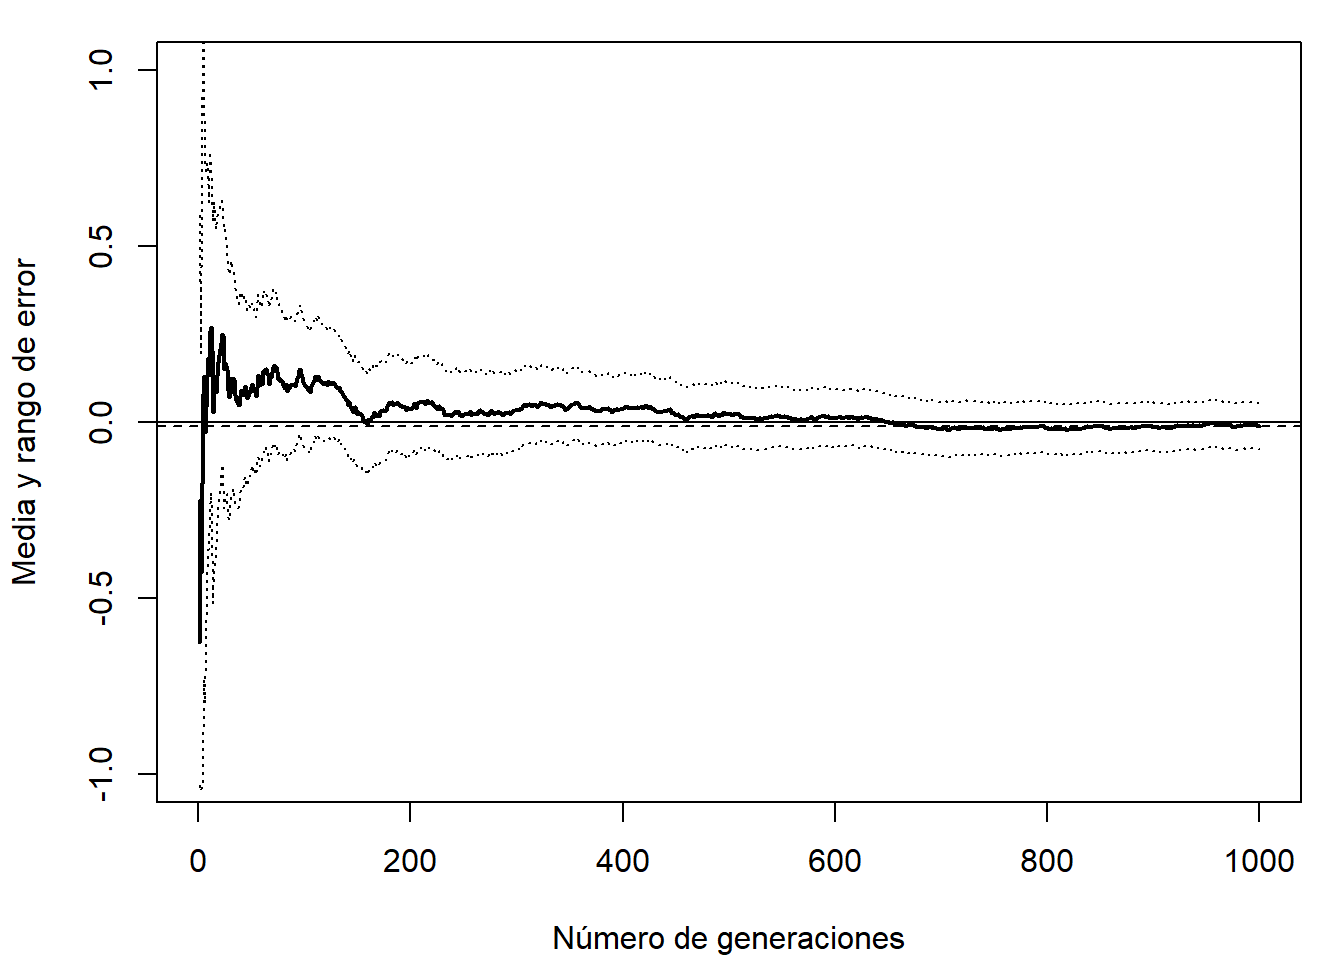
\includegraphics[width=0.7\linewidth]{04-Analisis_resultados_files/figure-latex/conv-esterr-1} 

}

\caption{Gráfico de convergencia incluyendo el error de la aproximación.}\label{fig:conv-esterr}
\end{figure}

\hypertarget{determinaciuxf3n-del-nuxfamero-de-generaciones}{%
\section{Determinación del número de generaciones}\label{determinaciuxf3n-del-nuxfamero-de-generaciones}}

Normalmente el valor de \(n\) se toma del orden de varias centenas o millares.
En los casos en los que la simulación se utiliza para aproximar una característica central de la distribución (como una media) puede bastar un número de simulaciones del orden de \(n = 100, 200, 500\).
Sin embargo, en otros casos pueden ser necesarios valores del tipo \(n = 1000, 2000, 5000, 10000\).

En muchas ocasiones puede interesar obtener una aproximación con un nivel de precisión fijado.
Para una precisión absoluta \(\varepsilon\), se trata de determinar
\(n\) de forma que:
\[z_{1-\alpha /2}\dfrac{\widehat{S}_{n}}{\sqrt{n}}<\varepsilon\]

Un algoritmo podría ser el siguiente:

\begin{enumerate}
\def\labelenumi{\arabic{enumi}.}
\item
  Hacer \(j=0\)
  y fijar un tamaño inicial \(n_{0}\) (e.g.~30 ó 60).
\item
  Generar \(\left\{ X_{i}\right\} _{i=1}^{n_{0}}\)
  y calcular \(\overline{X}_{n_0}\) y \(\widehat{S}_{n_{0}}\).
\item
  Mientras \(\left. z_{1-\alpha /2}\widehat{S}_{n_j}\right/ \sqrt{n_{j}}>\varepsilon\) hacer:

  3.1. \(j=j+1\).

  3.2. \(n_{j}=\left\lceil \left( \left. z_{1-\alpha /2}\widehat{S}  _{n_{j-1}}\right/ \varepsilon \right)^{2}\right\rceil\).

  3.3. Generar \(\left\{ X_{i}\right\}_{i=n_{j-1}+1}^{n_j}\)
  y calcular \(\overline{X}_{n_j}\) y \(\widehat{S}_{n_j}\).
\item
  Devolver \(\overline{X}_{n_j}\) y \(\left. z_{1-\alpha /2}\widehat{S}_{n_j}\right/ \sqrt{n_{j}}\).
\end{enumerate}

Para una precisión relativa \(\varepsilon \left\vert \mu \right\vert\) se procede análogamente de forma que:
\[z_{1-\alpha /2}\dfrac{\widehat{S}_{n}}{\sqrt{n}}<\varepsilon \left\vert 
\overline{X}_{n}\right\vert .\]

\hypertarget{el-problema-de-la-dependencia}{%
\section{El problema de la dependencia}\label{el-problema-de-la-dependencia}}

En el caso de dependencia, la estimación de la precisión se complica:
\[Var\left( \overline{X}\right) =\frac{1}{n^{2}}\left( 
\sum_{i=1}^{n}Var\left( X_{i} \right) + 2\sum_{i<j}Cov\left( X_{i},X_{j}\right) \right).\]

\begin{example}
\protect\hypertarget{exm:mmc}{}{\label{exm:mmc} }Aproximación de una proporción bajo dependencia (cadena de Markov)
\end{example}
Supongamos que en A Coruña llueve de media 1/3 días al año,
y que la probabilidad de que un día llueva solo depende de lo que ocurrió el día anterior,
siendo 0.94 si el día anterior llovió y 0.03 si no.
Podemos generar valores de la variable indicadora de día lluvioso con el siguiente código:

\begin{Shaded}
\begin{Highlighting}[]
\CommentTok{# Variable dicotómica 0/1 (FALSE/TRUE)  }
\KeywordTok{set.seed}\NormalTok{(}\DecValTok{1}\NormalTok{)}
\NormalTok{nsim <-}\StringTok{ }\DecValTok{10000}
\NormalTok{alpha <-}\StringTok{ }\FloatTok{0.03} \CommentTok{# prob de cambio si seco}
\NormalTok{beta <-}\StringTok{ }\FloatTok{0.06}  \CommentTok{# prob de cambio si lluvia}
\NormalTok{rx <-}\StringTok{ }\KeywordTok{logical}\NormalTok{(nsim) }\CommentTok{# x == "llueve"}
\NormalTok{rx[}\DecValTok{1}\NormalTok{] <-}\StringTok{ }\OtherTok{FALSE} \CommentTok{# El primer día no llueve}
\ControlFlowTok{for}\NormalTok{ (i }\ControlFlowTok{in} \DecValTok{2}\OperatorTok{:}\NormalTok{nsim)}
\NormalTok{  rx[i] <-}\StringTok{ }\ControlFlowTok{if}\NormalTok{ (rx[i}\DecValTok{-1}\NormalTok{]) }\KeywordTok{runif}\NormalTok{(}\DecValTok{1}\NormalTok{) }\OperatorTok{>}\StringTok{ }\NormalTok{beta }\ControlFlowTok{else} \KeywordTok{runif}\NormalTok{(}\DecValTok{1}\NormalTok{) }\OperatorTok{<}\StringTok{ }\NormalTok{alpha}
\end{Highlighting}
\end{Shaded}

Se podría pensar en emplear las expresiones anteriores:

\begin{Shaded}
\begin{Highlighting}[]
\NormalTok{n <-}\StringTok{ }\DecValTok{1}\OperatorTok{:}\NormalTok{nsim}
\NormalTok{est <-}\StringTok{ }\KeywordTok{cumsum}\NormalTok{(rx)}\OperatorTok{/}\NormalTok{n}
\NormalTok{esterr <-}\StringTok{ }\KeywordTok{sqrt}\NormalTok{(est}\OperatorTok{*}\NormalTok{(}\DecValTok{1}\OperatorTok{-}\NormalTok{est)}\OperatorTok{/}\NormalTok{(n}\DecValTok{-1}\NormalTok{)) }\CommentTok{# OJO! Supone independencia}
\KeywordTok{plot}\NormalTok{(est, }\DataTypeTok{type=}\StringTok{"l"}\NormalTok{, }\DataTypeTok{lwd=}\DecValTok{2}\NormalTok{, }\DataTypeTok{ylab=}\StringTok{"Probabilidad"}\NormalTok{, }
     \DataTypeTok{xlab=}\StringTok{"Número de simulaciones"}\NormalTok{, }\DataTypeTok{ylim=}\KeywordTok{c}\NormalTok{(}\DecValTok{0}\NormalTok{,}\FloatTok{0.6}\NormalTok{))}
\KeywordTok{abline}\NormalTok{(}\DataTypeTok{h =}\NormalTok{ est[nsim], }\DataTypeTok{lty=}\DecValTok{2}\NormalTok{)}
\KeywordTok{lines}\NormalTok{(est }\OperatorTok{+}\StringTok{ }\DecValTok{2}\OperatorTok{*}\NormalTok{esterr, }\DataTypeTok{lty=}\DecValTok{2}\NormalTok{) }
\KeywordTok{lines}\NormalTok{(est }\OperatorTok{-}\StringTok{ }\DecValTok{2}\OperatorTok{*}\NormalTok{esterr, }\DataTypeTok{lty=}\DecValTok{2}\NormalTok{)}
\KeywordTok{abline}\NormalTok{(}\DataTypeTok{h =} \DecValTok{1}\OperatorTok{/}\DecValTok{3}\NormalTok{, }\DataTypeTok{col=}\StringTok{"darkgray"}\NormalTok{)     }\CommentTok{# Prob. teor. cadenas Markov}
\end{Highlighting}
\end{Shaded}

\begin{figure}[!htb]

{\centering 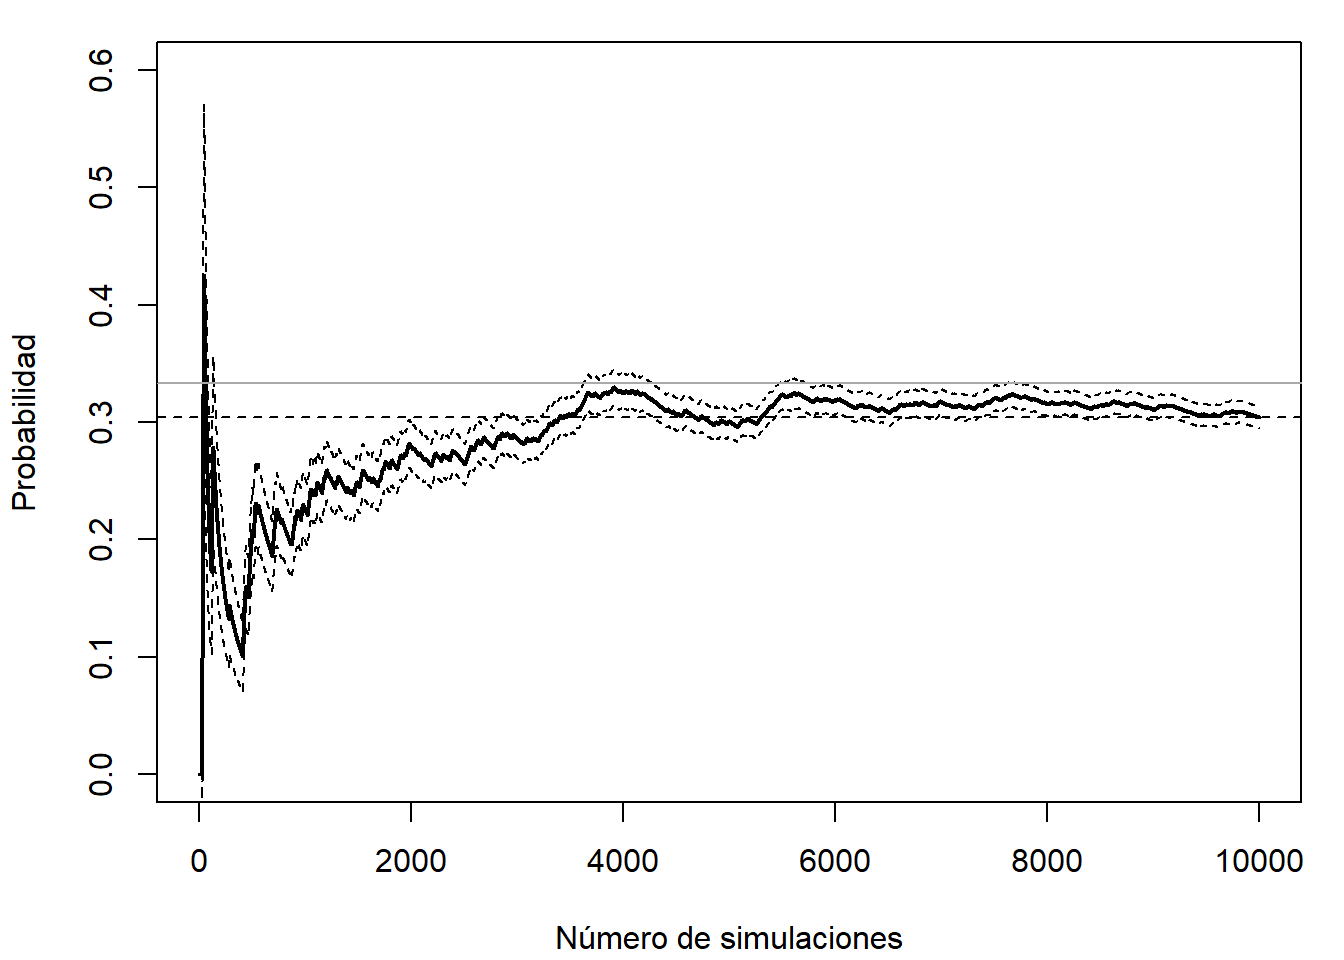
\includegraphics[width=0.7\linewidth]{04-Analisis_resultados_files/figure-latex/conv-dep-1} 

}

\caption{Gráfico de convergencia incluyendo el error de la aproximación (calculado asumiendo independencia).}\label{fig:conv-dep}
\end{figure}

La aproximación de la proporción sería correcta (es consistente):

\begin{Shaded}
\begin{Highlighting}[]
\NormalTok{est[nsim]}
\end{Highlighting}
\end{Shaded}

\begin{verbatim}
## [1] 0.3038
\end{verbatim}

Sin embargo, al ser datos dependientes esta aproximación del error estandar no es adecuada:

\begin{Shaded}
\begin{Highlighting}[]
\NormalTok{esterr[nsim]}
\end{Highlighting}
\end{Shaded}

\begin{verbatim}
## [1] 0.004599203
\end{verbatim}

En este caso al haber dependencia positiva se produce una
subestimación del verdadero error estandar.

\begin{Shaded}
\begin{Highlighting}[]
\KeywordTok{acf}\NormalTok{(}\KeywordTok{as.numeric}\NormalTok{(rx))}
\end{Highlighting}
\end{Shaded}

\begin{figure}[!htb]

{\centering 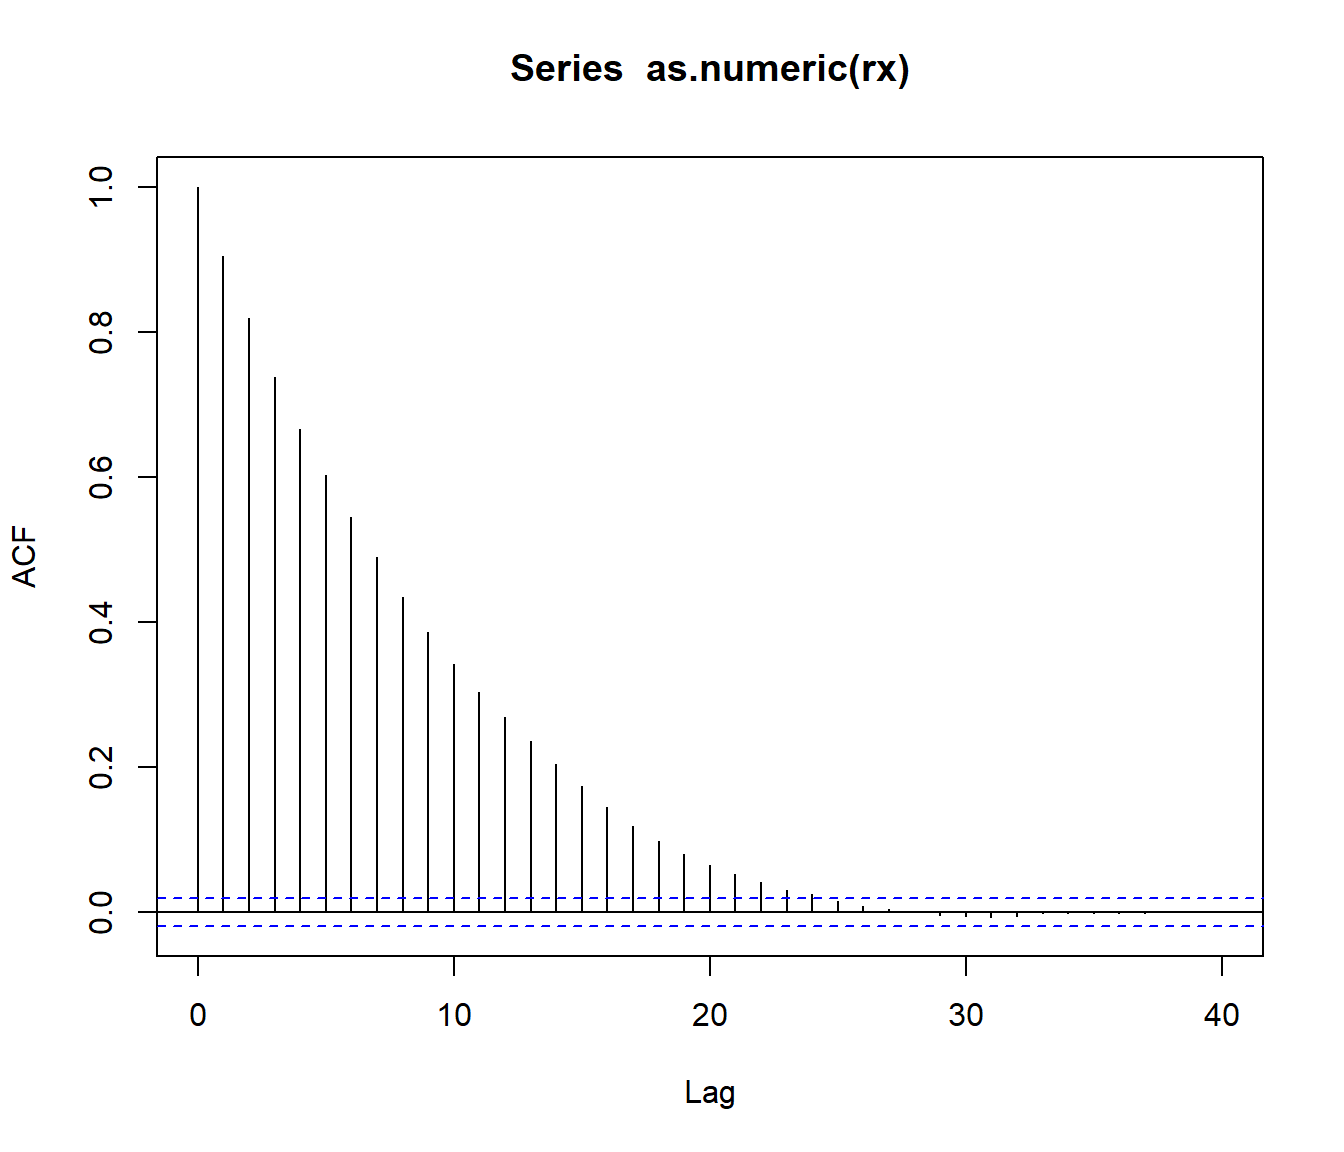
\includegraphics[width=0.7\linewidth]{04-Analisis_resultados_files/figure-latex/acf-depsec-1} 

}

\caption{Correlograma de la secuencia indicadora de días de lluvia.}\label{fig:acf-depsec}
\end{figure}

El gráfico de autocorrelaciones sugiere que si tomamos 1 de cada 25
podemos suponer independencia.

\begin{Shaded}
\begin{Highlighting}[]
\NormalTok{lag <-}\StringTok{ }\DecValTok{24}
\NormalTok{xlag <-}\StringTok{ }\KeywordTok{c}\NormalTok{(}\KeywordTok{rep}\NormalTok{(}\OtherTok{FALSE}\NormalTok{, lag), }\OtherTok{TRUE}\NormalTok{)}
\NormalTok{rxi <-}\StringTok{ }\NormalTok{rx[xlag]}
\KeywordTok{acf}\NormalTok{(}\KeywordTok{as.numeric}\NormalTok{(rxi))}
\end{Highlighting}
\end{Shaded}

\begin{figure}[!htb]

{\centering 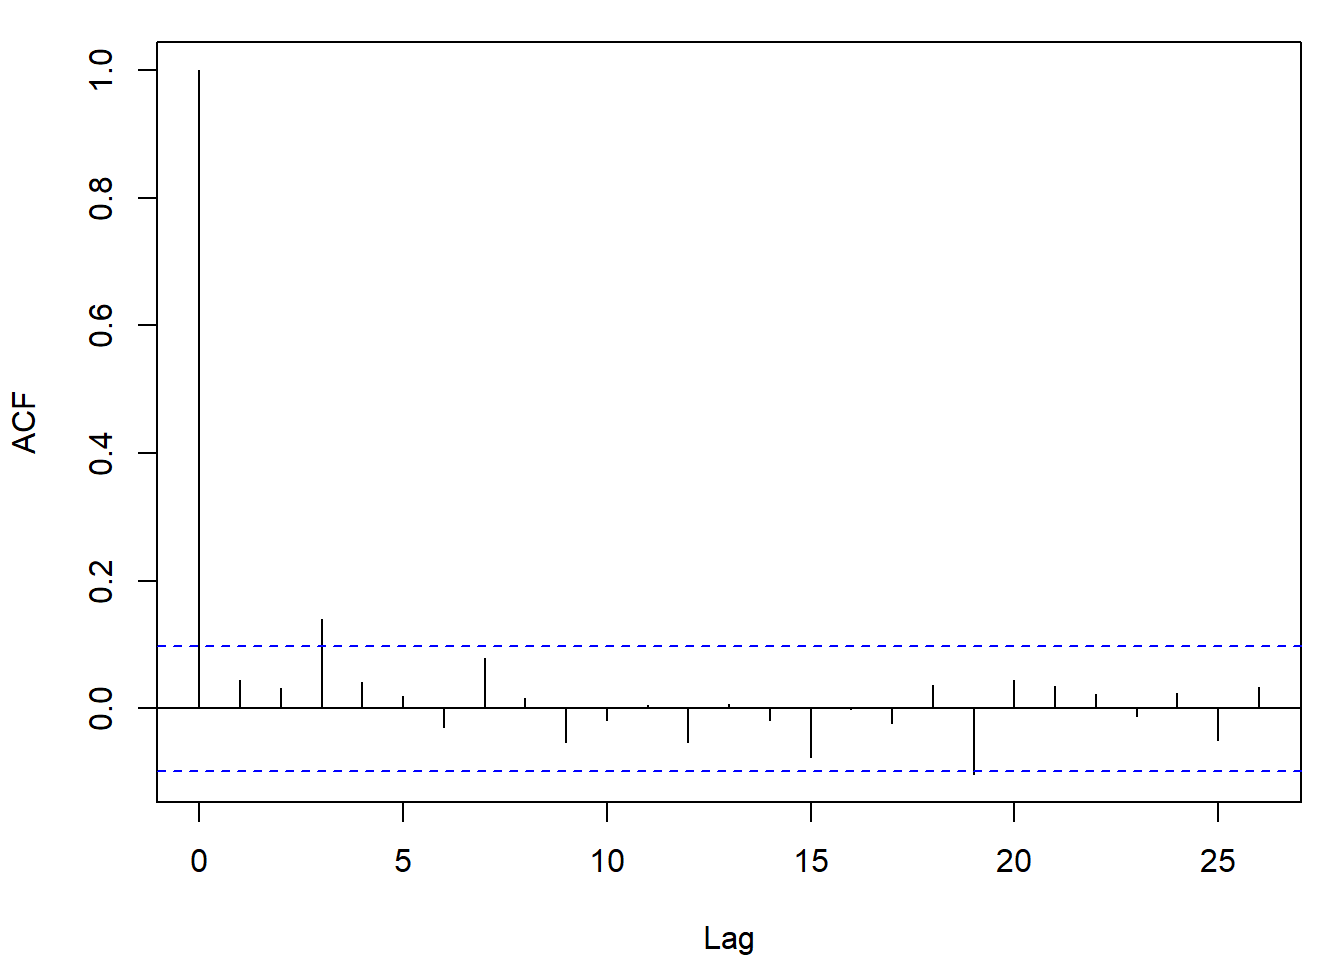
\includegraphics[width=0.7\linewidth]{04-Analisis_resultados_files/figure-latex/acf-depsec2-1} 

}

\caption{Correlograma de la subsecuencia de días de lluvia obtenida seleccionando uno de cada 25 valores.}\label{fig:acf-depsec2}
\end{figure}

\begin{Shaded}
\begin{Highlighting}[]
\NormalTok{nrxi <-}\StringTok{ }\KeywordTok{length}\NormalTok{(rxi)}
\NormalTok{n <-}\StringTok{ }\DecValTok{1}\OperatorTok{:}\NormalTok{nrxi}
\NormalTok{est <-}\StringTok{ }\KeywordTok{cumsum}\NormalTok{(rxi)}\OperatorTok{/}\NormalTok{n}
\NormalTok{esterr <-}\StringTok{ }\KeywordTok{sqrt}\NormalTok{(est}\OperatorTok{*}\NormalTok{(}\DecValTok{1}\OperatorTok{-}\NormalTok{est)}\OperatorTok{/}\NormalTok{(n}\DecValTok{-1}\NormalTok{))}
\KeywordTok{plot}\NormalTok{(est, }\DataTypeTok{type=}\StringTok{"l"}\NormalTok{, }\DataTypeTok{lwd=}\DecValTok{2}\NormalTok{, }\DataTypeTok{ylab=}\StringTok{"Probabilidad"}\NormalTok{, }
     \DataTypeTok{xlab=}\KeywordTok{paste}\NormalTok{(}\StringTok{"Número de simulaciones /"}\NormalTok{, lag }\OperatorTok{+}\StringTok{ }\DecValTok{1}\NormalTok{), }\DataTypeTok{ylim=}\KeywordTok{c}\NormalTok{(}\DecValTok{0}\NormalTok{,}\FloatTok{0.6}\NormalTok{))}
\KeywordTok{abline}\NormalTok{(}\DataTypeTok{h =}\NormalTok{ est[}\KeywordTok{length}\NormalTok{(rxi)], }\DataTypeTok{lty=}\DecValTok{2}\NormalTok{)}
\KeywordTok{lines}\NormalTok{(est }\OperatorTok{+}\StringTok{ }\DecValTok{2}\OperatorTok{*}\NormalTok{esterr, }\DataTypeTok{lty=}\DecValTok{2}\NormalTok{) }\CommentTok{# Supone independencia}
\KeywordTok{lines}\NormalTok{(est }\OperatorTok{-}\StringTok{ }\DecValTok{2}\OperatorTok{*}\NormalTok{esterr, }\DataTypeTok{lty=}\DecValTok{2}\NormalTok{)}
\KeywordTok{abline}\NormalTok{(}\DataTypeTok{h =} \DecValTok{1}\OperatorTok{/}\DecValTok{3}\NormalTok{, }\DataTypeTok{col=}\StringTok{"darkgray"}\NormalTok{)     }\CommentTok{# Prob. teor. cadenas Markov}
\end{Highlighting}
\end{Shaded}

\begin{figure}[!htb]

{\centering 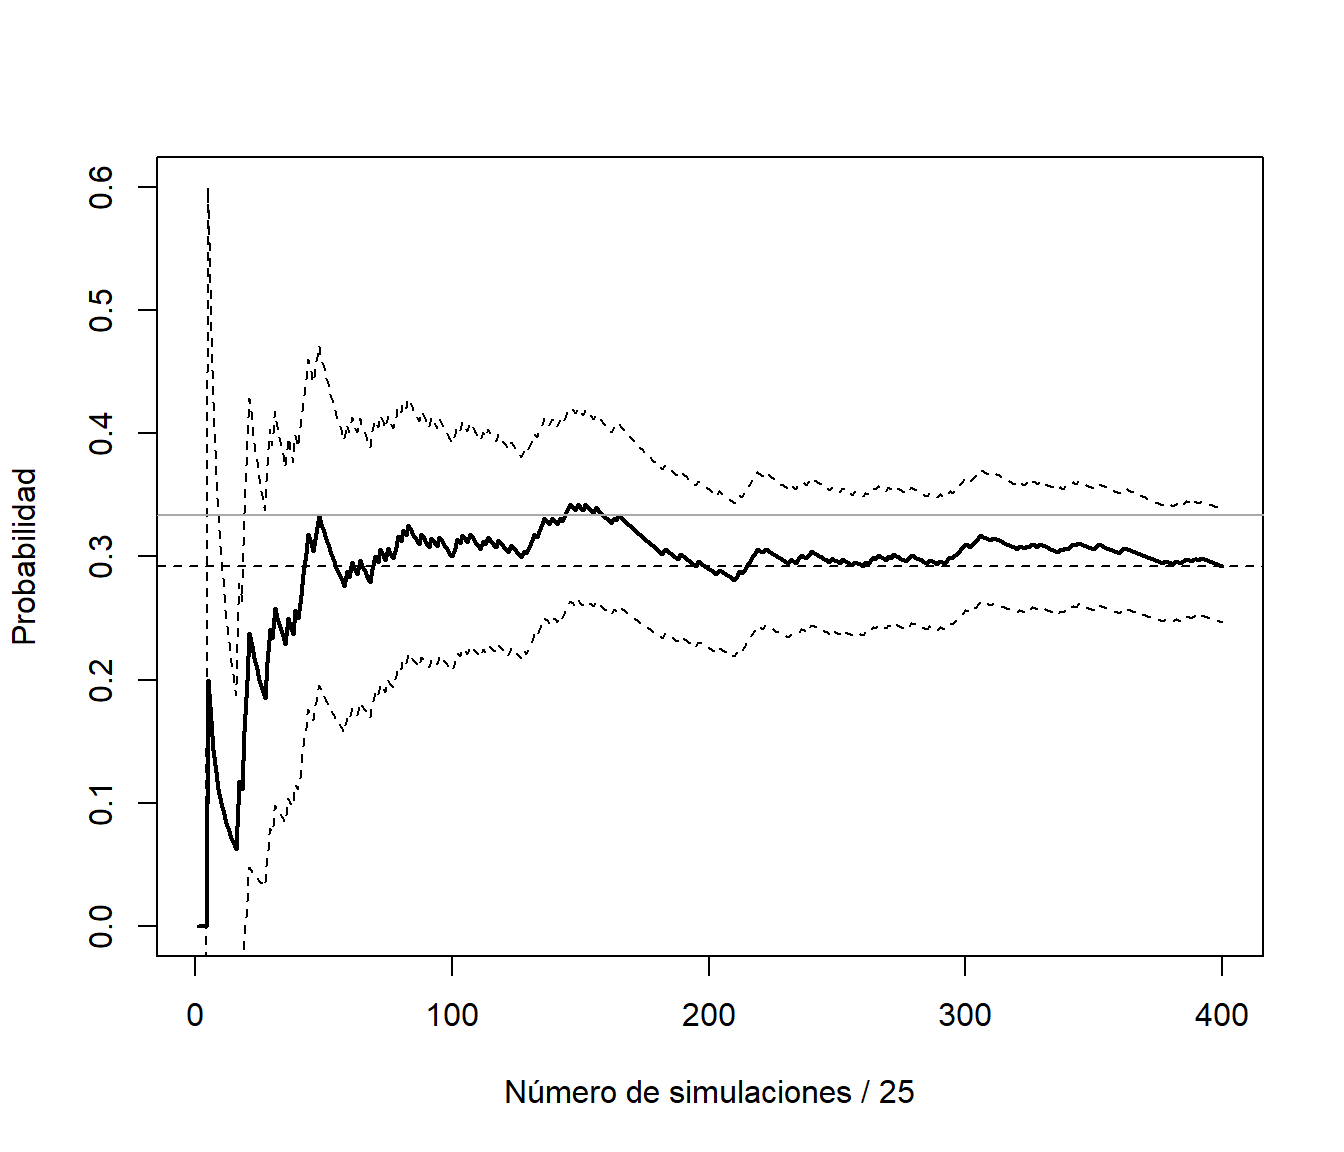
\includegraphics[width=0.7\linewidth]{04-Analisis_resultados_files/figure-latex/conv-dep2-1} 

}

\caption{Gráfico de convergencia de la aproximación de la probabilidad a partir de la subsecuencia de días de lluvia (calculando el error de aproximación asumiendo independencia).}\label{fig:conv-dep2}
\end{figure}

Esta forma de proceder podría ser adecuada para tratar de aproximar la precisión:

\begin{Shaded}
\begin{Highlighting}[]
\NormalTok{esterr[nrxi]}
\end{Highlighting}
\end{Shaded}

\begin{verbatim}
## [1] 0.02277402
\end{verbatim}

pero no sería eficiente para aproximar la media. Siempre será preferible emplear
todas las observaciones.

Por ejemplo, se podría pensar en considerar las medias de grupos de 24 valores
consecutivos y suponer que hay independencia entre ellas:

\begin{Shaded}
\begin{Highlighting}[]
\NormalTok{rxm <-}\StringTok{ }\KeywordTok{rowMeans}\NormalTok{(}\KeywordTok{matrix}\NormalTok{(rx, }\DataTypeTok{ncol =}\NormalTok{ lag, }\DataTypeTok{byrow =} \OtherTok{TRUE}\NormalTok{))}
\NormalTok{nrxm <-}\StringTok{ }\KeywordTok{length}\NormalTok{(rxm)}
\NormalTok{n <-}\StringTok{ }\DecValTok{1}\OperatorTok{:}\NormalTok{nrxm}
\NormalTok{est <-}\StringTok{ }\KeywordTok{cumsum}\NormalTok{(rxm)}\OperatorTok{/}\NormalTok{n}
\NormalTok{esterr <-}\StringTok{ }\KeywordTok{sqrt}\NormalTok{(}\KeywordTok{cumsum}\NormalTok{((rxm}\OperatorTok{-}\NormalTok{est)}\OperatorTok{^}\DecValTok{2}\NormalTok{))}\OperatorTok{/}\NormalTok{n  }\CommentTok{# Error estándar}
\KeywordTok{plot}\NormalTok{(est, }\DataTypeTok{type=}\StringTok{"l"}\NormalTok{, }\DataTypeTok{lwd=}\DecValTok{2}\NormalTok{, }\DataTypeTok{ylab=}\StringTok{"Probabilidad"}\NormalTok{, }
     \DataTypeTok{xlab=}\KeywordTok{paste}\NormalTok{(}\StringTok{"Número de simulaciones /"}\NormalTok{, lag }\OperatorTok{+}\StringTok{ }\DecValTok{1}\NormalTok{), }\DataTypeTok{ylim=}\KeywordTok{c}\NormalTok{(}\DecValTok{0}\NormalTok{,}\FloatTok{0.6}\NormalTok{))}
\KeywordTok{abline}\NormalTok{(}\DataTypeTok{h =}\NormalTok{ est[}\KeywordTok{length}\NormalTok{(rxm)], }\DataTypeTok{lty=}\DecValTok{2}\NormalTok{)}
\KeywordTok{lines}\NormalTok{(est }\OperatorTok{+}\StringTok{ }\DecValTok{2}\OperatorTok{*}\NormalTok{esterr, }\DataTypeTok{lty=}\DecValTok{2}\NormalTok{) }\CommentTok{# OJO! Supone independencia}
\KeywordTok{lines}\NormalTok{(est }\OperatorTok{-}\StringTok{ }\DecValTok{2}\OperatorTok{*}\NormalTok{esterr, }\DataTypeTok{lty=}\DecValTok{2}\NormalTok{)}
\KeywordTok{abline}\NormalTok{(}\DataTypeTok{h =} \DecValTok{1}\OperatorTok{/}\DecValTok{3}\NormalTok{, }\DataTypeTok{col=}\StringTok{"darkgray"}\NormalTok{)     }\CommentTok{# Prob. teor. cadenas Markov}
\end{Highlighting}
\end{Shaded}

\begin{figure}[!htb]

{\centering 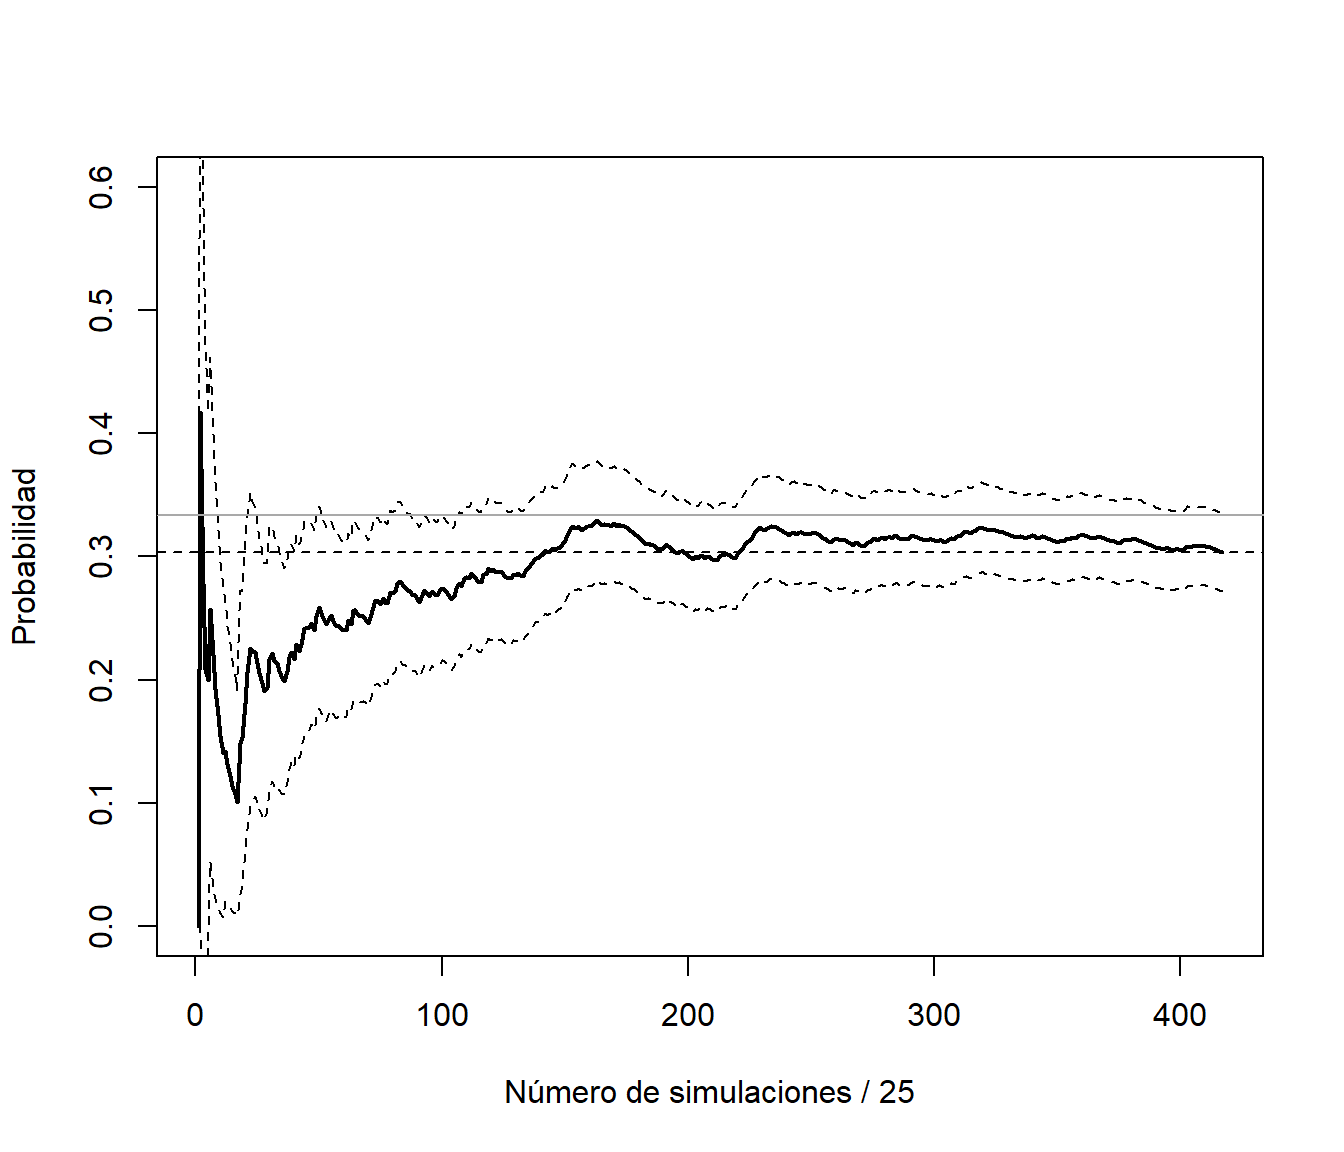
\includegraphics[width=0.7\linewidth]{04-Analisis_resultados_files/figure-latex/conv-dep-lotes-1} 

}

\caption{Gráfico de convergencia de las medias por lotes.}\label{fig:conv-dep-lotes}
\end{figure}

Esta es la idea del método de medias por lotes
(\emph{batch means}; \emph{macro-micro replicaciones}) para la estimación de la varianza.
En el ejemplo anterior se calcula el error estándar de la aproximación por simulación de la proporción:

\begin{Shaded}
\begin{Highlighting}[]
\NormalTok{esterr[nrxm]}
\end{Highlighting}
\end{Shaded}

\begin{verbatim}
## [1] 0.01569017
\end{verbatim}

pero si el objetivo es la aproximación de la varianza (de la variable y no de las medias por lotes), habrá que reescalarlo adecuadamente.
Supongamos que la correlación entre \(X_i\) y \(X_{i+k}\) es aproximadamente nula,
y consideramos las subsecuencias (lotes) \((X_{t+1},X_{t+2},\ldots,X_{t+k})\) con \(t=(j-1)k\), \(j=1,\ldots,m\) y \(n = mk\).
Entonces:

\[\begin{aligned}
Var \left(\bar X \right) &= Var \left(\frac{1}{n} \sum_{i=1}^n X_i\right) 
= Var \left( \frac{1}{m}\sum_{j=1}^m \left(\frac{1}{k} \sum_{t=(i-1)k + 1}^{ik} X_t\right) \right) \\
&\approx \frac{1}{m^2} \sum_{j=1}^m Var \left(\frac{1}{k} \sum_{t=(i-1)k + 1}^{ik} X_t\right)
\approx \frac{1}{m} Var \left(\bar{X}_k \right)
\end{aligned}\]
donde \(\bar{X}_k\) es la media de una subsecuencia de longitud \(k\).

\begin{Shaded}
\begin{Highlighting}[]
\NormalTok{var.aprox <-}\StringTok{ }\NormalTok{nsim }\OperatorTok{*}\StringTok{ }\NormalTok{esterr[}\KeywordTok{length}\NormalTok{(rxm)]}\OperatorTok{^}\DecValTok{2}
\NormalTok{var.aprox}
\end{Highlighting}
\end{Shaded}

\begin{verbatim}
## [1] 2.461814
\end{verbatim}

Obtenida asumiendo independencia entre las medias por lotes, y que será
una mejor aproximación que asumir independencia entre las generaciones
de la variable:

\begin{Shaded}
\begin{Highlighting}[]
\KeywordTok{var}\NormalTok{(rx)}
\end{Highlighting}
\end{Shaded}

\begin{verbatim}
## [1] 0.2115267
\end{verbatim}

Alternativamente se podría recurrir a la generación de múltiples secuencias
independientes entre sí:

\begin{Shaded}
\begin{Highlighting}[]
\CommentTok{# Variable dicotómica 0/1 (FALSE/TRUE)  }
\KeywordTok{set.seed}\NormalTok{(}\DecValTok{1}\NormalTok{)}
\NormalTok{nsim <-}\StringTok{ }\DecValTok{1000}
\NormalTok{nsec <-}\StringTok{ }\DecValTok{10}
\NormalTok{alpha <-}\StringTok{ }\FloatTok{0.03} \CommentTok{# prob de cambio si seco}
\NormalTok{beta <-}\StringTok{ }\FloatTok{0.06}  \CommentTok{# prob de cambio si lluvia}
\NormalTok{rxm <-}\StringTok{ }\KeywordTok{matrix}\NormalTok{(}\OtherTok{FALSE}\NormalTok{, }\DataTypeTok{nrow =}\NormalTok{ nsec, }\DataTypeTok{ncol=}\NormalTok{ nsim)}
\ControlFlowTok{for}\NormalTok{ (i }\ControlFlowTok{in} \DecValTok{1}\OperatorTok{:}\NormalTok{nsec) \{}
  \CommentTok{# rxm[i, 1] <- FALSE # El primer día no llueve}
  \CommentTok{# rxm[i, 1] <- runif(1) < 1/2 # El primer día llueve con probabilidad 1/2}
\NormalTok{  rxm[i, }\DecValTok{1}\NormalTok{] <-}\StringTok{ }\KeywordTok{runif}\NormalTok{(}\DecValTok{1}\NormalTok{) }\OperatorTok{<}\StringTok{ }\DecValTok{1}\OperatorTok{/}\DecValTok{3} \CommentTok{# El primer día llueve con probabilidad 1/3 (ideal)}
  \ControlFlowTok{for}\NormalTok{ (j }\ControlFlowTok{in} \DecValTok{2}\OperatorTok{:}\NormalTok{nsim)}
\NormalTok{    rxm[i, j] <-}\StringTok{ }\ControlFlowTok{if}\NormalTok{ (rxm[i, j}\DecValTok{-1}\NormalTok{]) }\KeywordTok{runif}\NormalTok{(}\DecValTok{1}\NormalTok{) }\OperatorTok{>}\StringTok{ }\NormalTok{beta }\ControlFlowTok{else} \KeywordTok{runif}\NormalTok{(}\DecValTok{1}\NormalTok{) }\OperatorTok{<}\StringTok{ }\NormalTok{alpha}
\NormalTok{\}}
\end{Highlighting}
\end{Shaded}

La idea sería considerar las medias de las series como una muestra independiente
de una nueva variable y estimar su varianza de la forma habitual:

\begin{Shaded}
\begin{Highlighting}[]
\CommentTok{# Media de cada secuencia}
\NormalTok{n <-}\StringTok{ }\DecValTok{1}\OperatorTok{:}\NormalTok{nsim}
\NormalTok{est <-}\StringTok{ }\KeywordTok{apply}\NormalTok{(rxm, }\DecValTok{1}\NormalTok{, }\ControlFlowTok{function}\NormalTok{(x) }\KeywordTok{cumsum}\NormalTok{(x)}\OperatorTok{/}\NormalTok{n)}
\KeywordTok{matplot}\NormalTok{(n, est, }\DataTypeTok{type =} \StringTok{'l'}\NormalTok{, }\DataTypeTok{lty =} \DecValTok{3}\NormalTok{, }\DataTypeTok{col =} \StringTok{"lightgray"}\NormalTok{,}
     \DataTypeTok{ylab=}\StringTok{"Probabilidad"}\NormalTok{, }\DataTypeTok{xlab=}\StringTok{"Número de simulaciones"}\NormalTok{)}
\CommentTok{# Aproximación}
\NormalTok{mest <-}\StringTok{ }\KeywordTok{apply}\NormalTok{(est, }\DecValTok{1}\NormalTok{, mean)}
\KeywordTok{lines}\NormalTok{(mest, }\DataTypeTok{lwd =} \DecValTok{2}\NormalTok{)}
\KeywordTok{abline}\NormalTok{(}\DataTypeTok{h =}\NormalTok{ mest[nsim], }\DataTypeTok{lty =} \DecValTok{2}\NormalTok{)}
\CommentTok{# Precisión}
\NormalTok{mesterr <-}\StringTok{ }\KeywordTok{apply}\NormalTok{(est, }\DecValTok{1}\NormalTok{, sd)}\OperatorTok{/}\KeywordTok{sqrt}\NormalTok{(nsec)}
\KeywordTok{lines}\NormalTok{(mest }\OperatorTok{+}\StringTok{ }\DecValTok{2}\OperatorTok{*}\NormalTok{mesterr, }\DataTypeTok{lty =} \DecValTok{2}\NormalTok{)}
\KeywordTok{lines}\NormalTok{(mest }\OperatorTok{-}\StringTok{ }\DecValTok{2}\OperatorTok{*}\NormalTok{mesterr, }\DataTypeTok{lty =} \DecValTok{2}\NormalTok{)}
\CommentTok{# Prob. teor. cadenas Markov}
\KeywordTok{abline}\NormalTok{(}\DataTypeTok{h =} \DecValTok{1}\OperatorTok{/}\DecValTok{3}\NormalTok{, }\DataTypeTok{col=}\StringTok{"darkgray"}\NormalTok{)     }
\end{Highlighting}
\end{Shaded}

\begin{figure}[!htb]

{\centering 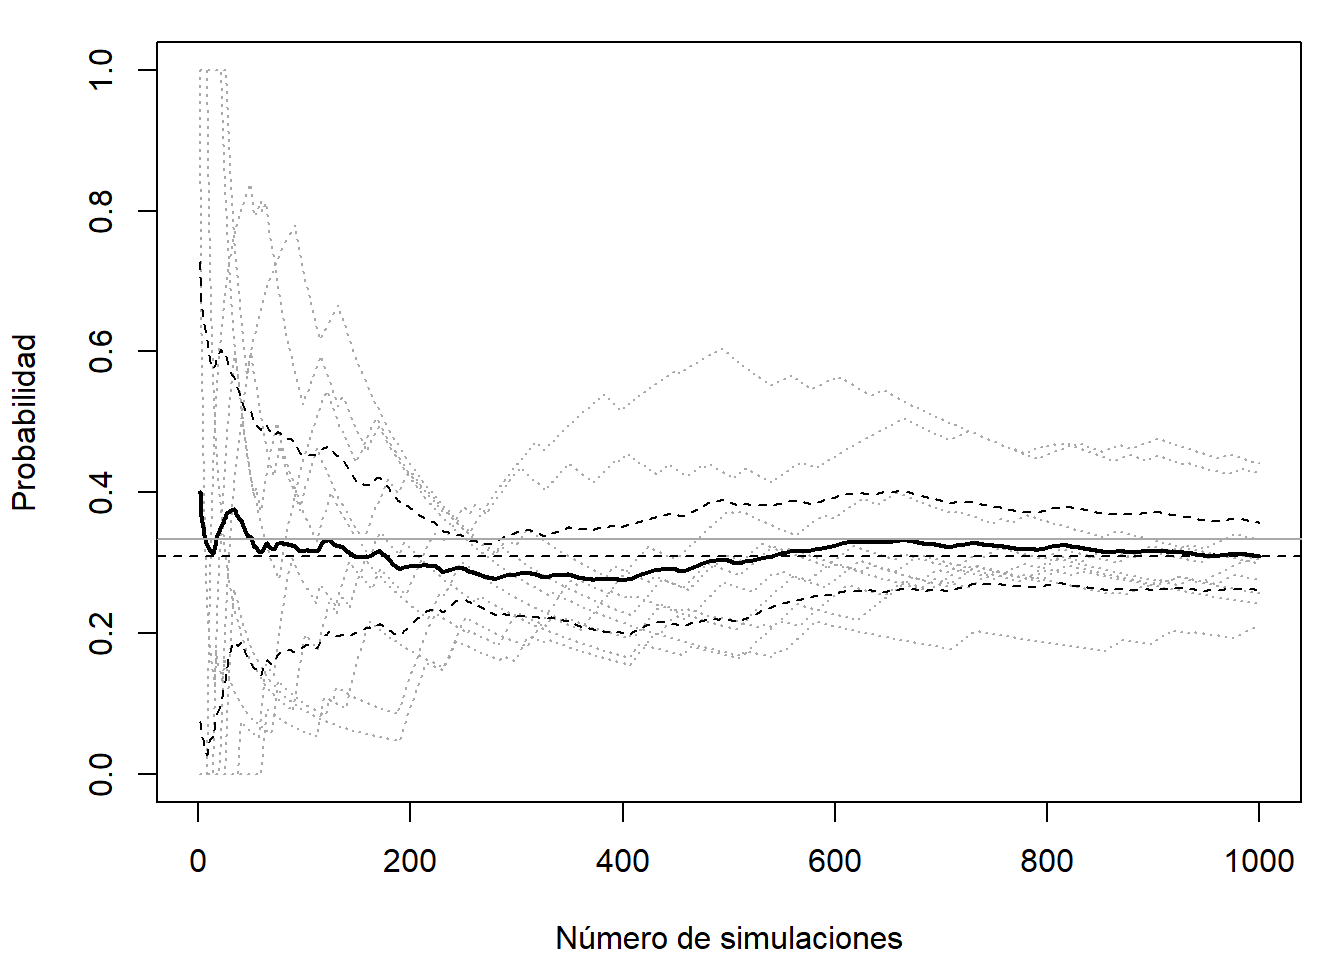
\includegraphics[width=0.7\linewidth]{04-Analisis_resultados_files/figure-latex/conv-dep-nsec-1} 

}

\caption{Gráfico de convergencia de la media de 10 secuencias generadas de forma independiente.}\label{fig:conv-dep-nsec}
\end{figure}

\begin{Shaded}
\begin{Highlighting}[]
\CommentTok{# Aproximación final}
\NormalTok{mest[nsim] }\CommentTok{# mean(rxm)}
\end{Highlighting}
\end{Shaded}

\begin{verbatim}
## [1] 0.3089
\end{verbatim}

\begin{Shaded}
\begin{Highlighting}[]
\CommentTok{# Error estándar}
\NormalTok{mesterr[nsim]}
\end{Highlighting}
\end{Shaded}

\begin{verbatim}
## [1] 0.02403491
\end{verbatim}

Trataremos este tipo de problemas en la diagnosis de algoritmos de
simulación Monte Carlo de Cadenas de Markov (MCMC).
Aparecen también en la simulación dinámica (por eventos o cuantos).

\hypertarget{periodo-de-calentamiento}{%
\subsection{Periodo de calentamiento}\label{periodo-de-calentamiento}}

En el caso de simulación de datos dependientes (simulación dinámica)
pueden aparecer problemas de estabilización. Puede ocurrir que el sistema
evolucione lentamente en el tiempo hasta alcanzar su distribución estacionaria,
siendo muy sensible a las condiciones iniciales con las que se comienzó la
simulación. En tal caso resulta conveniente ignorar los resultados obtenidos
durante un cierto período inicial de tiempo (denominado período de calentamiento
o estabilización), cuyo único objeto es conseguir que se estabilice la distribución de
probabilidad.

Como ejemplo comparamos la simulación del Ejemplo \ref{exm:mmc} con la obtenida considerando como punto de partida un día lluvioso (con una semilla distinta para evitar dependencia).

\begin{Shaded}
\begin{Highlighting}[]
\KeywordTok{set.seed}\NormalTok{(}\DecValTok{2}\NormalTok{)}
\NormalTok{nsim <-}\StringTok{ }\DecValTok{10000}
\NormalTok{rx2 <-}\StringTok{ }\KeywordTok{logical}\NormalTok{(nsim)}
\NormalTok{rx2[}\DecValTok{1}\NormalTok{] <-}\StringTok{ }\OtherTok{TRUE} \CommentTok{# El primer día llueve}
\ControlFlowTok{for}\NormalTok{ (i }\ControlFlowTok{in} \DecValTok{2}\OperatorTok{:}\NormalTok{nsim)}
\NormalTok{  rx2[i] <-}\StringTok{ }\ControlFlowTok{if}\NormalTok{ (rx2[i}\DecValTok{-1}\NormalTok{]) }\KeywordTok{runif}\NormalTok{(}\DecValTok{1}\NormalTok{) }\OperatorTok{>}\StringTok{ }\NormalTok{beta }\ControlFlowTok{else} \KeywordTok{runif}\NormalTok{(}\DecValTok{1}\NormalTok{) }\OperatorTok{<}\StringTok{ }\NormalTok{alpha}
\NormalTok{n <-}\StringTok{ }\DecValTok{1}\OperatorTok{:}\NormalTok{nsim}
\NormalTok{est <-}\StringTok{ }\KeywordTok{cumsum}\NormalTok{(rx)}\OperatorTok{/}\NormalTok{n}
\NormalTok{est2 <-}\StringTok{ }\KeywordTok{cumsum}\NormalTok{(rx2)}\OperatorTok{/}\NormalTok{n}
\KeywordTok{plot}\NormalTok{(est, }\DataTypeTok{type=}\StringTok{"l"}\NormalTok{, }\DataTypeTok{ylab=}\StringTok{"Probabilidad"}\NormalTok{, }
     \DataTypeTok{xlab=}\StringTok{"Número de simulaciones"}\NormalTok{, }\DataTypeTok{ylim=}\KeywordTok{c}\NormalTok{(}\DecValTok{0}\NormalTok{,}\FloatTok{0.6}\NormalTok{))}
\KeywordTok{lines}\NormalTok{(est2, }\DataTypeTok{lty =} \DecValTok{2}\NormalTok{)}
\CommentTok{# Ejemplo periodo calentamiento nburn = 2000}
\KeywordTok{abline}\NormalTok{(}\DataTypeTok{v =} \DecValTok{2000}\NormalTok{, }\DataTypeTok{lty =} \DecValTok{3}\NormalTok{)}
\CommentTok{# Prob. teor. cadenas Markov}
\KeywordTok{abline}\NormalTok{(}\DataTypeTok{h =} \DecValTok{1}\OperatorTok{/}\DecValTok{3}\NormalTok{, }\DataTypeTok{col=}\StringTok{"darkgray"}\NormalTok{)     }
\end{Highlighting}
\end{Shaded}

\begin{center}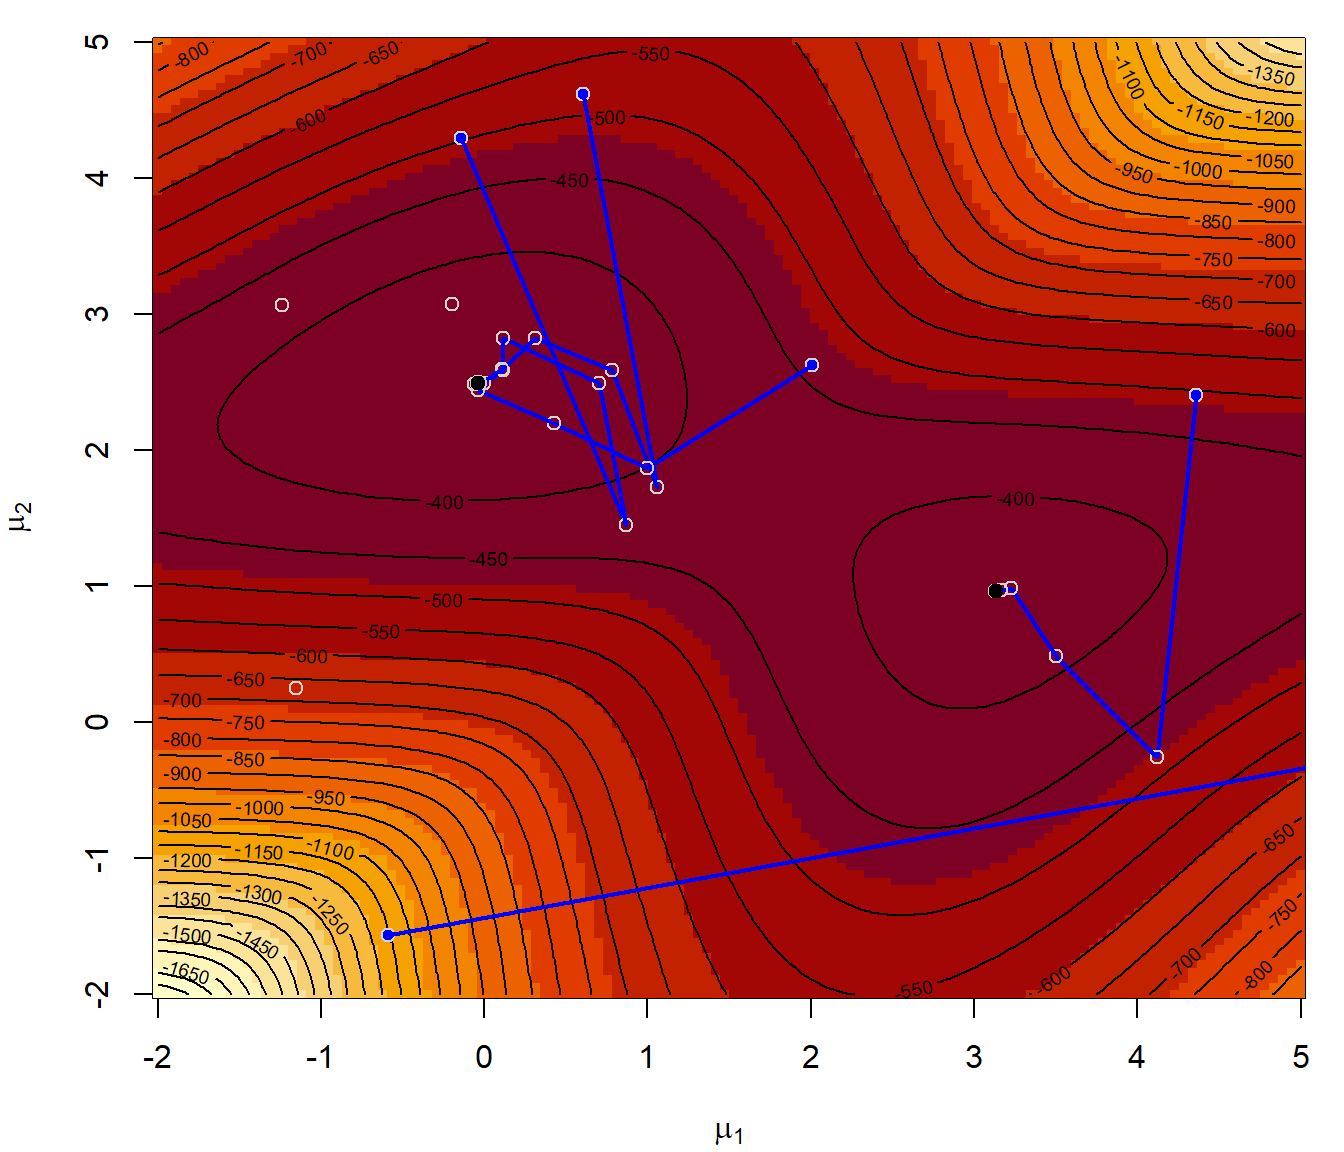
\includegraphics[width=0.7\linewidth]{04-Analisis_resultados_files/figure-latex/unnamed-chunk-17-1} \end{center}

En estos casos puede ser recomendable ignorar los primeros valores generados (por ejemplo los primeros 2000) y recalcular los
estadísticos deseados.

También trataremos este tipo de problemas en la diagnosis de algoritmos MCMC.

\begin{example}
\protect\hypertarget{exm:unnamed-chunk-18}{}{\label{exm:unnamed-chunk-18} }Simulación de un proceso autorregresivo (serie de tiempo)
\end{example}

\[X_t = \mu + \rho * (X_{t-1} - \mu) + \varepsilon_t\]
Podemos tener en cuenta que en este caso la varianza es:
\[\textrm{var}(X_t)=\operatorname{E}(X_t^2)-\mu^2=\frac{\sigma_\varepsilon^2}{1-\rho^2}.\]

Establecemos los parámetros:

\begin{Shaded}
\begin{Highlighting}[]
\NormalTok{nsim <-}\StringTok{ }\DecValTok{200}   \CommentTok{# Numero de simulaciones}
\NormalTok{xmed <-}\StringTok{ }\DecValTok{0}     \CommentTok{# Media}
\NormalTok{rho <-}\StringTok{ }\FloatTok{0.5}    \CommentTok{# Coeficiente AR}
\NormalTok{nburn <-}\StringTok{ }\DecValTok{10}   \CommentTok{# Periodo de calentamiento (burn-in)}
\end{Highlighting}
\end{Shaded}

Se podría fijar la varianza del error:

\begin{Shaded}
\begin{Highlighting}[]
\NormalTok{evar <-}\StringTok{ }\DecValTok{1}
\CommentTok{# Varianza de la respuesta}
\NormalTok{xvar <-}\StringTok{ }\NormalTok{evar }\OperatorTok{/}\StringTok{ }\NormalTok{(}\DecValTok{1} \OperatorTok{-}\StringTok{ }\NormalTok{rho}\OperatorTok{^}\DecValTok{2}\NormalTok{)}
\end{Highlighting}
\end{Shaded}

pero la recomendación sería fijar la varianza de la respuesta:

\begin{Shaded}
\begin{Highlighting}[]
\NormalTok{xvar <-}\StringTok{ }\DecValTok{1}     
\CommentTok{# Varianza del error}
\NormalTok{evar <-}\StringTok{ }\NormalTok{xvar}\OperatorTok{*}\NormalTok{(}\DecValTok{1} \OperatorTok{-}\StringTok{ }\NormalTok{rho}\OperatorTok{^}\DecValTok{2}\NormalTok{)}
\end{Highlighting}
\end{Shaded}

Para simular la serie, al ser un \(AR(1)\), normalmente simularíamos el primer valor

\begin{Shaded}
\begin{Highlighting}[]
\NormalTok{rx[}\DecValTok{1}\NormalTok{] <-}\StringTok{ }\KeywordTok{rnorm}\NormalTok{(}\DecValTok{1}\NormalTok{, }\DataTypeTok{mean =}\NormalTok{ xmed, }\DataTypeTok{sd =} \KeywordTok{sqrt}\NormalTok{(xvar))}
\end{Highlighting}
\end{Shaded}

o lo fijamos a la media (en este caso nos alejamos un poco de la distribución estacionaria, para que el ``periodo de calentamiento'' sea mayor).
Después generamos los siguientes valores de forma recursiva:

\begin{Shaded}
\begin{Highlighting}[]
\KeywordTok{set.seed}\NormalTok{(}\DecValTok{1}\NormalTok{)}
\NormalTok{x <-}\StringTok{ }\KeywordTok{numeric}\NormalTok{(nsim }\OperatorTok{+}\StringTok{ }\NormalTok{nburn)}
\CommentTok{# Establecer el primer valor }
\NormalTok{x[}\DecValTok{1}\NormalTok{] <-}\StringTok{ }\DecValTok{-10}
\CommentTok{# Simular el resto de la secuencia}
\ControlFlowTok{for}\NormalTok{ (i }\ControlFlowTok{in} \DecValTok{2}\OperatorTok{:}\KeywordTok{length}\NormalTok{(x))}
\NormalTok{  x[i] <-}\StringTok{ }\NormalTok{xmed }\OperatorTok{+}\StringTok{ }\NormalTok{rho}\OperatorTok{*}\NormalTok{(x[i}\DecValTok{-1}\NormalTok{] }\OperatorTok{-}\StringTok{ }\NormalTok{xmed) }\OperatorTok{+}\StringTok{ }\KeywordTok{rnorm}\NormalTok{(}\DecValTok{1}\NormalTok{, }\DataTypeTok{sd=}\KeywordTok{sqrt}\NormalTok{(evar))}
\NormalTok{x <-}\StringTok{ }\KeywordTok{as.ts}\NormalTok{(x)}
\KeywordTok{plot}\NormalTok{(x)}
\KeywordTok{abline}\NormalTok{(}\DataTypeTok{v =}\NormalTok{ nburn, }\DataTypeTok{lty =} \DecValTok{2}\NormalTok{)}
\end{Highlighting}
\end{Shaded}

\begin{figure}[!htb]

{\centering 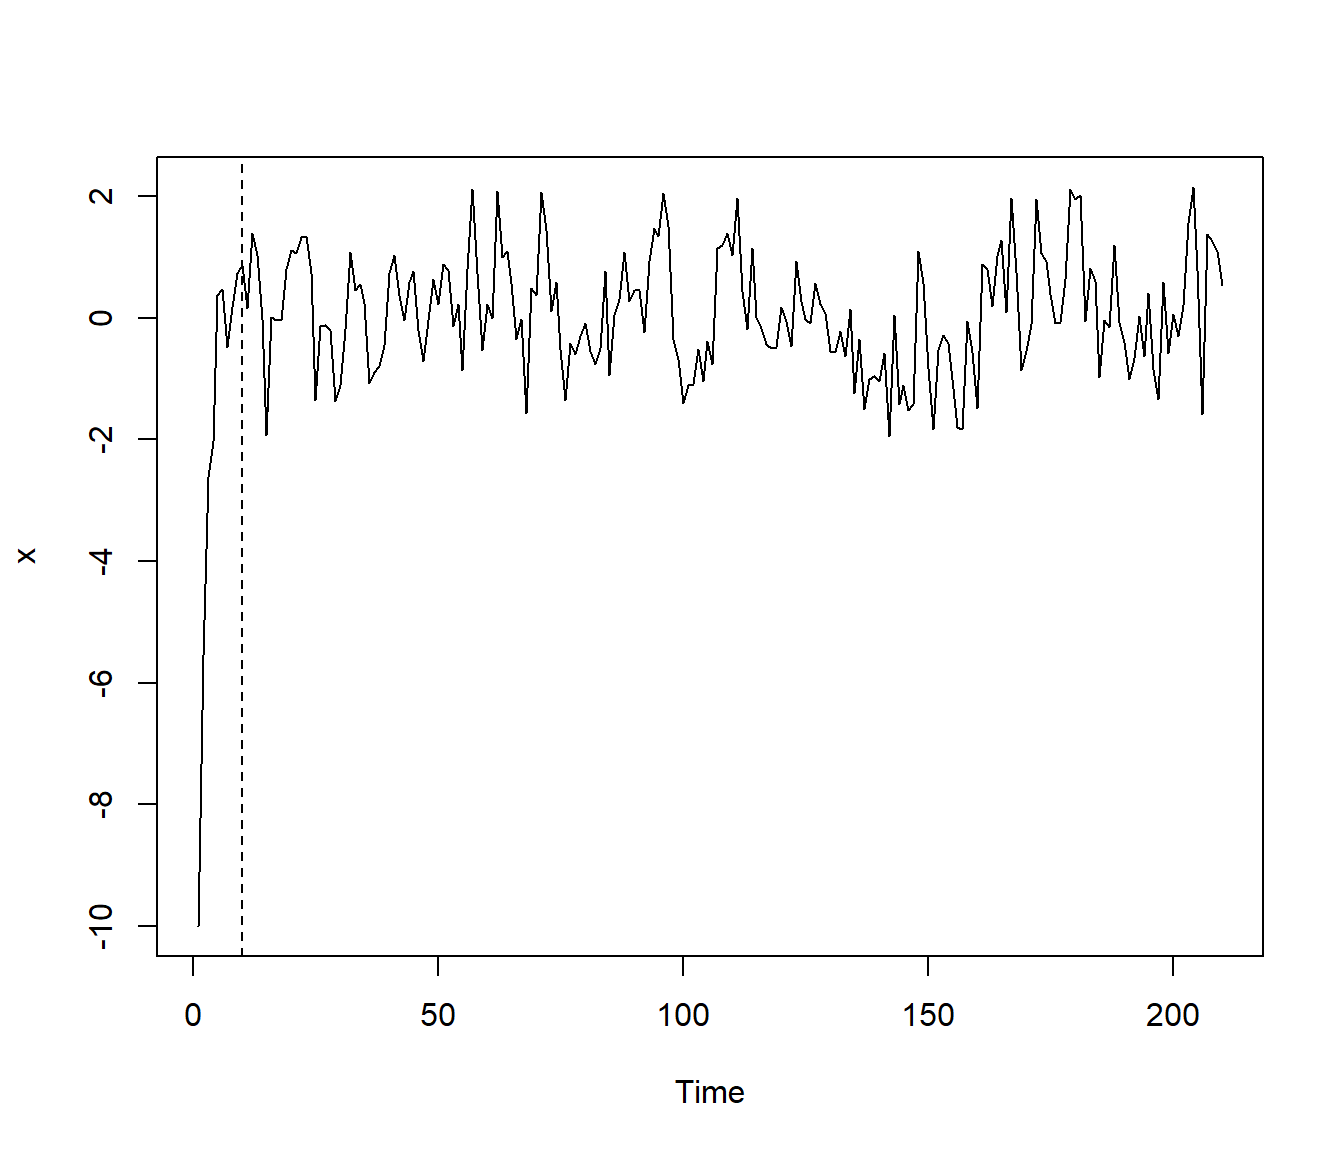
\includegraphics[width=0.7\linewidth]{04-Analisis_resultados_files/figure-latex/sim-ar1-1} 

}

\caption{Ejemplo de una simulación de una serie de tiempo autorregresiva.}\label{fig:sim-ar1}
\end{figure}

y eliminamos el periodo de calentamiento:

\begin{Shaded}
\begin{Highlighting}[]
\NormalTok{rx <-}\StringTok{ }\NormalTok{x[}\OperatorTok{-}\KeywordTok{seq_len}\NormalTok{(nburn)]}
\end{Highlighting}
\end{Shaded}

Para simular una serie de tiempo en \texttt{R}
se puede emplear la función \texttt{arima.sim} del paquete base \texttt{stats}.
En este caso el periodo de calentamiento se establece mediante el
parámetro \texttt{n.start} (que se fija automáticamente a un valor adecuado).

Por ejemplo, podemos generar este serie autoregressiva con:

\begin{Shaded}
\begin{Highlighting}[]
\NormalTok{rx2 <-}\StringTok{ }\KeywordTok{arima.sim}\NormalTok{(}\KeywordTok{list}\NormalTok{(}\DataTypeTok{order =} \KeywordTok{c}\NormalTok{(}\DecValTok{1}\NormalTok{,}\DecValTok{0}\NormalTok{,}\DecValTok{0}\NormalTok{), }\DataTypeTok{ar =}\NormalTok{ rho), }\DataTypeTok{n =}\NormalTok{ nsim, }\DataTypeTok{n.start =}\NormalTok{ nburn, }\DataTypeTok{sd =} \KeywordTok{sqrt}\NormalTok{(evar))}
\end{Highlighting}
\end{Shaded}

La recomendación es fijar la varianza de las series simuladas si se quieren comparar
resultados considerando distintos parámetros de dependencia.

\hypertarget{observaciones}{%
\section{Observaciones}\label{observaciones}}

\begin{itemize}
\item
  En el caso de que la característica de interés de la
  distribución de \(X\) no sea la media, los resultados anteriores
  no serían en principio aplicables.
\item
  Incluso en el caso de la media, las ``bandas de confianza''
  obtenidas con el TCL son puntuales (si generamos nuevas
  secuencias de simulación es muy probable que no
  estén contenidas).
\item
  En muchos casos (p.e. la generación de múltiples secuencias de
  simulación puede suponer un coste computacional importante),
  puede ser preferible emplear un método de remuestreo.
\end{itemize}

\hypertarget{sim-con}{%
\chapter{Simulación de variables continuas}\label{sim-con}}

En este capítulo se expondrán métodos generales para simular distribuciones continuas: el método de inversión y los basados en aceptación/rechazo.
En todos los casos como punto de partida es necesario
disponer de un método de generación de números pseudoaleatorios uniformes en \((0,1)\).

\hypertarget{muxe9todo-de-inversiuxf3n}{%
\section{Método de inversión}\label{muxe9todo-de-inversiuxf3n}}

Se trataría del método preferible para la simulación de una variable continua (siempre que se disponga de la función cuantil).
Está basado en los siguientes resultados:

Si \(X\) es una variable aleatoria con función de distribución \(F\) continua y estrictamente monótona
(invertible), entonces:
\[U=F\left( X \right) \sim \mathcal{U}(0, 1)\]
ya que:
\[G\left( u \right) = P\left( Y \leq u \right) 
= P\left( F(X) \leq u \right) \\
= P\left( X \leq F^{-1}(u) \right) 
= F\left( F^{-1}(u) \right) = u\]

El recíproco también es cierto, si \(U \sim \mathcal{U}(0, 1)\) entonces:
\[F^{-1}\left( U \right) \sim X\]

A partir de este resultado se deduce el siguiente algoritmo genérico para simular una variable continua con función de distribución \(F\) invertible:

\begin{conjecture}[Método de inversión]
\protect\hypertarget{cnj:inversion}{}{\label{cnj:inversion} \iffalse (Método de inversión) \fi{} }
1. Generar \(U \sim \mathcal{U}(0, 1)\).

\begin{enumerate}
\def\labelenumi{\arabic{enumi}.}
\setcounter{enumi}{1}
\tightlist
\item
  Devolver \(X = F^{-1}\left( U \right)\).
\end{enumerate}
\end{conjecture}

\begin{example}[Simulación de una distribución exponencial]
\protect\hypertarget{exm:exp-inv}{}{\label{exm:exp-inv} \iffalse (Simulación de una distribución exponencial) \fi{} }
\end{example}

La distribución exponencial \(\exp \left( \lambda \right)\) de parámetro \(\lambda>0\)
tiene como función de densidad \(f(x) =\lambda e^{-\lambda x}\), si \(x\geq 0\),
y como función de distribución:
\[F(x)=\left\{ \begin{array}{ll}
1-e^{-\lambda x} & \text{si } x \ge 0 \\
0 & \text{si } x < 0\\
\end{array} \right.\]
Teniendo en cuenta que:
\[1-e^{-\lambda x}=u \Leftrightarrow x=-\frac{\ln \left( 1-u\right) }{ \lambda }\]
el algoritmo para simular esta variable mediante el método de inversión es:

\begin{enumerate}
\def\labelenumi{\arabic{enumi}.}
\item
  Generar \(U \sim \mathcal{U}(0, 1)\).
\item
  Devolver \(X=-\dfrac{\ln \left( 1-U\right) }{\lambda }\).
\end{enumerate}

En el último paso podemos emplear directamente \(U\) en lugar de \(1-U\), ya que \(1 - U \sim \mathcal{U}(0, 1)\).
Esta última expresión para acelerar los cálculos es la que denominaremos \emph{forma simplificada}.

\begin{figure}[!htb]

{\centering \includegraphics[width=0.7\linewidth]{05-Metodos_generales_continuas_files/figure-latex/inv-movie-1} 

}

\caption{Ilustración de la simulación de una distribución exponencial por el método de inversión.}\label{fig:inv-movie}
\end{figure}

El código para implementar este algoritmo en R podría ser el siguiente:

\begin{Shaded}
\begin{Highlighting}[]
\NormalTok{tini <-}\StringTok{ }\KeywordTok{proc.time}\NormalTok{()}

\NormalTok{lambda <-}\StringTok{ }\DecValTok{2}
\NormalTok{nsim <-}\StringTok{ }\DecValTok{10}\OperatorTok{^}\DecValTok{5}
\KeywordTok{set.seed}\NormalTok{(}\DecValTok{1}\NormalTok{)}
\NormalTok{U <-}\StringTok{ }\KeywordTok{runif}\NormalTok{(nsim)}
\NormalTok{X <-}\StringTok{ }\OperatorTok{-}\KeywordTok{log}\NormalTok{(U)}\OperatorTok{/}\NormalTok{lambda }\CommentTok{# -log(1-U)/lambda}

\NormalTok{tiempo <-}\StringTok{ }\KeywordTok{proc.time}\NormalTok{() }\OperatorTok{-}\StringTok{ }\NormalTok{tini}
\NormalTok{tiempo}
\end{Highlighting}
\end{Shaded}

\begin{verbatim}
##    user  system elapsed 
##    0.01    0.00    0.01
\end{verbatim}

\begin{Shaded}
\begin{Highlighting}[]
\KeywordTok{hist}\NormalTok{(X, }\DataTypeTok{breaks =} \StringTok{"FD"}\NormalTok{, }\DataTypeTok{freq =} \OtherTok{FALSE}\NormalTok{, }
        \DataTypeTok{main =} \StringTok{""}\NormalTok{, }\DataTypeTok{xlim =} \KeywordTok{c}\NormalTok{(}\DecValTok{0}\NormalTok{, }\DecValTok{5}\NormalTok{), }\DataTypeTok{ylim =} \KeywordTok{c}\NormalTok{(}\DecValTok{0}\NormalTok{, }\FloatTok{2.5}\NormalTok{))}
\KeywordTok{curve}\NormalTok{(}\KeywordTok{dexp}\NormalTok{(x, lambda), }\DataTypeTok{lwd =} \DecValTok{2}\NormalTok{, }\DataTypeTok{add =} \OtherTok{TRUE}\NormalTok{)}
\end{Highlighting}
\end{Shaded}

\begin{figure}[!htb]

{\centering 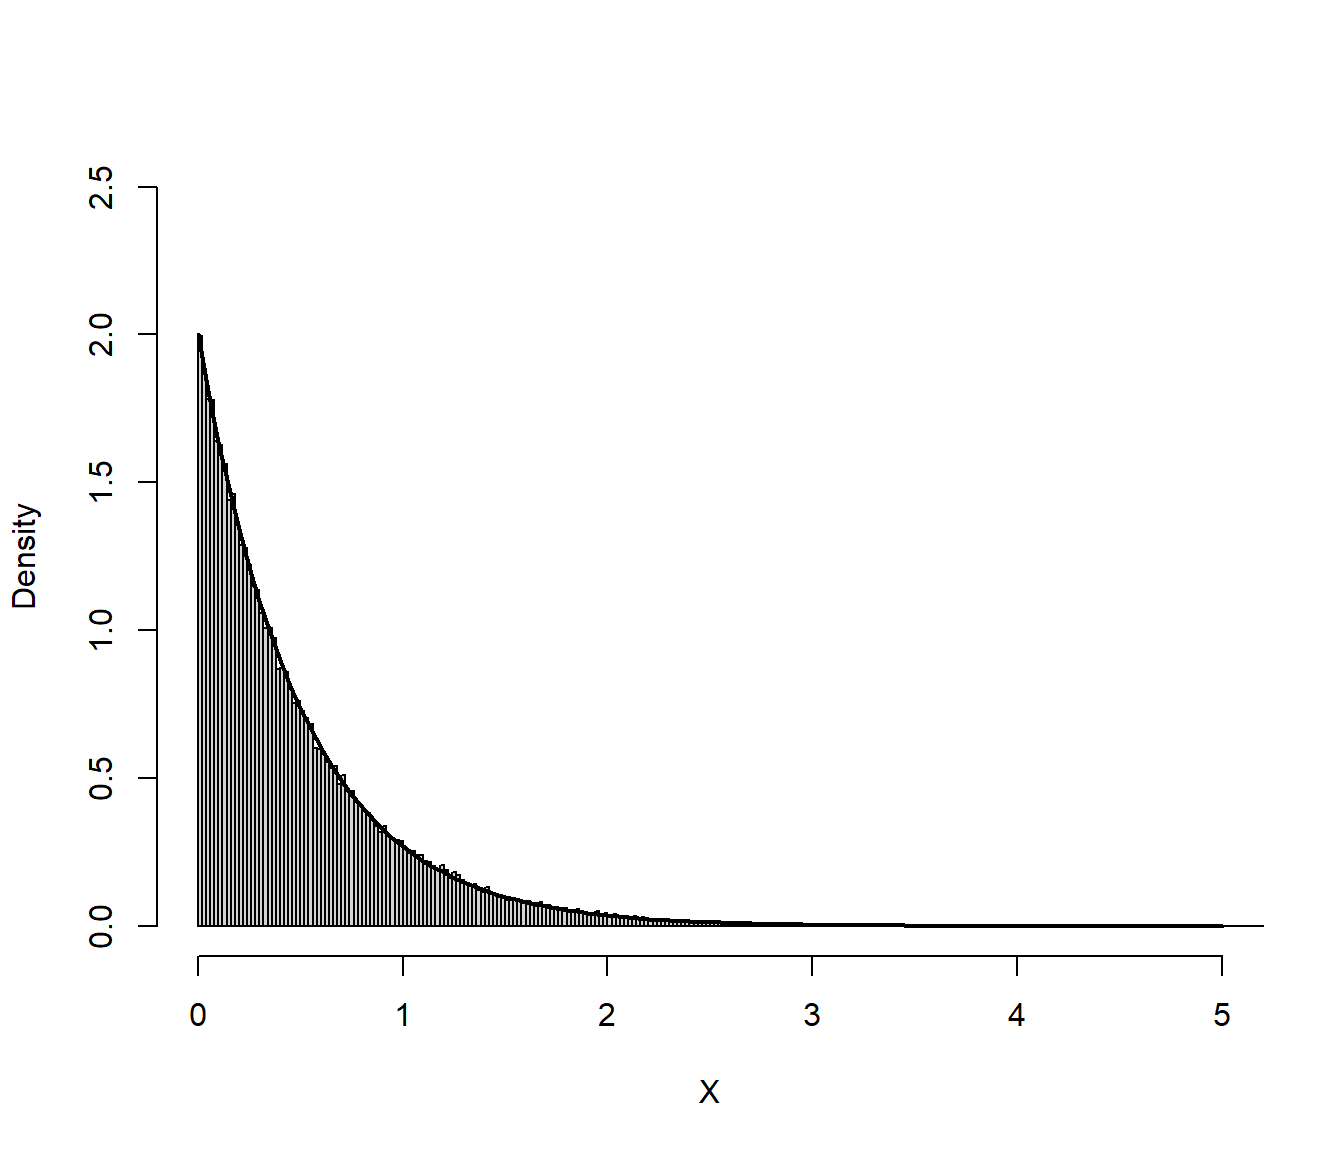
\includegraphics[width=0.7\linewidth]{05-Metodos_generales_continuas_files/figure-latex/exp-inv-plot-1} 

}

\caption{Distribución de los valores generados de una exponencial mediante el método de inversión.}\label{fig:exp-inv-plot}
\end{figure}

Como se observa en la Figura \ref{fig:exp-inv-plot} se trata de un método exacto (si está bien implementado) y la distribución de los valores generados se aproxima a la distribución teórica como cabría esperar con una muestra de ese tamaño.

\hypertarget{algunas-distribuciones-que-pueden-simularse-por-el-muxe9todo-de-inversiuxf3n}{%
\subsection{Algunas distribuciones que pueden simularse por el método de inversión}\label{algunas-distribuciones-que-pueden-simularse-por-el-muxe9todo-de-inversiuxf3n}}

A continuación se incluyen algunas distribuciones que se pueden simular
fácilmente mediante el método de inversión. Se adjunta una forma
simplificada del método que tiene por objeto evitar cálculos
innecesarios (tal y como se hizo en el ejemplo de la exponencial).

\begin{longtable}[]{@{}lllll@{}}
\toprule
\begin{minipage}[b]{0.17\columnwidth}\raggedright
Nombre\strut
\end{minipage} & \begin{minipage}[b]{0.17\columnwidth}\raggedright
Densidad\strut
\end{minipage} & \begin{minipage}[b]{0.17\columnwidth}\raggedright
\(F(x)\)\strut
\end{minipage} & \begin{minipage}[b]{0.17\columnwidth}\raggedright
\(F^{-1}\left( U\right)\)\strut
\end{minipage} & \begin{minipage}[b]{0.17\columnwidth}\raggedright
Forma simplificada\strut
\end{minipage}\tabularnewline
\midrule
\endhead
\begin{minipage}[t]{0.17\columnwidth}\raggedright
\(\exp\left( \lambda\right)\) (\(\lambda>0\))\strut
\end{minipage} & \begin{minipage}[t]{0.17\columnwidth}\raggedright
\(\lambda e^{-\lambda x}\), si \(x\geq0\)\strut
\end{minipage} & \begin{minipage}[t]{0.17\columnwidth}\raggedright
\(1-e^{-\lambda x}\)\strut
\end{minipage} & \begin{minipage}[t]{0.17\columnwidth}\raggedright
\(-\dfrac{\ln\left( 1-U\right) }\lambda\)\strut
\end{minipage} & \begin{minipage}[t]{0.17\columnwidth}\raggedright
\(-\dfrac{\ln U}\lambda\)\strut
\end{minipage}\tabularnewline
\begin{minipage}[t]{0.17\columnwidth}\raggedright
Cauchy\strut
\end{minipage} & \begin{minipage}[t]{0.17\columnwidth}\raggedright
\(\dfrac1{\pi\left( 1+x^{2}\right) }\)\strut
\end{minipage} & \begin{minipage}[t]{0.17\columnwidth}\raggedright
\(\dfrac12+\dfrac{\arctan x}\pi\)\strut
\end{minipage} & \begin{minipage}[t]{0.17\columnwidth}\raggedright
\(\tan\left( \pi\left( U-\dfrac12\right) \right)\)\strut
\end{minipage} & \begin{minipage}[t]{0.17\columnwidth}\raggedright
\(\tan\pi U\)\strut
\end{minipage}\tabularnewline
\begin{minipage}[t]{0.17\columnwidth}\raggedright
Triangular en \(\left( 0,a\right)\)\strut
\end{minipage} & \begin{minipage}[t]{0.17\columnwidth}\raggedright
\(\dfrac2a\left( 1-\dfrac xa\right)\), si \(0\leq x\leq a\)\strut
\end{minipage} & \begin{minipage}[t]{0.17\columnwidth}\raggedright
\(\dfrac2a\left(x-\dfrac{x^{2}}{2a}\right)\)\strut
\end{minipage} & \begin{minipage}[t]{0.17\columnwidth}\raggedright
\(a\left( 1-\sqrt{1-U}\right)\)\strut
\end{minipage} & \begin{minipage}[t]{0.17\columnwidth}\raggedright
\(a\left( 1-\sqrt{U}\right)\)\strut
\end{minipage}\tabularnewline
\begin{minipage}[t]{0.17\columnwidth}\raggedright
Pareto (\(a,b>0\))\strut
\end{minipage} & \begin{minipage}[t]{0.17\columnwidth}\raggedright
\(\dfrac{ab^{a}}{x^{a+1}}\), si \(x\geq b\)\strut
\end{minipage} & \begin{minipage}[t]{0.17\columnwidth}\raggedright
\(1-\left( \dfrac bx\right)^{a}\)\strut
\end{minipage} & \begin{minipage}[t]{0.17\columnwidth}\raggedright
\(\dfrac b{\left( 1-U\right) ^{1/a}}\)\strut
\end{minipage} & \begin{minipage}[t]{0.17\columnwidth}\raggedright
\(\dfrac b{U^{1/a}}\)\strut
\end{minipage}\tabularnewline
\begin{minipage}[t]{0.17\columnwidth}\raggedright
Weibull (\(\lambda,\alpha>0\))\strut
\end{minipage} & \begin{minipage}[t]{0.17\columnwidth}\raggedright
\(\alpha\lambda^{\alpha}x^{\alpha-1}e^{-\left( \lambda x\right) ^{\alpha}}\), si \(x\geq0\)\strut
\end{minipage} & \begin{minipage}[t]{0.17\columnwidth}\raggedright
\(1-e^{-\left( \lambda x\right) ^{\alpha}}\)\strut
\end{minipage} & \begin{minipage}[t]{0.17\columnwidth}\raggedright
\(\dfrac{\left( -\ln\left(1-U\right) \right) ^{1/\alpha}}\lambda\)\strut
\end{minipage} & \begin{minipage}[t]{0.17\columnwidth}\raggedright
\(\dfrac{\left( -\ln U\right)^{1/\alpha}}\lambda\)\textbackslash{}\strut
\end{minipage}\tabularnewline
\bottomrule
\end{longtable}

\begin{exercise}[Distribución doble exponencial]
\protect\hypertarget{exr:ddexp}{}{\label{exr:ddexp} \iffalse (Distribución doble exponencial) \fi{} }
\end{exercise}

La distribución doble exponencial (o distribución de Laplace) de
parámetro \(\lambda\) tiene función de densidad:
\[f(x)  =\frac{\lambda}{2}e^{-\lambda\left\vert x\right\vert
}\text{, }x\in\mathbb{R}\]
y función de distribución:
\[F(x)  =\int_{-\infty}^{x}f\left( t\right)  dt=\left\{
\begin{array}{ll}
\frac{1}{2}e^{\lambda x} & \text{si } x<0\\
1-\frac{1}{2}e^{-\lambda x} & \text{si } x\geq0
\end{array}
\ \right.\]

\begin{enumerate}
\def\labelenumi{\alph{enumi})}
\item
  Escribir una función que permita generar, por el método de
  inversión, una muestra de \(n\) observaciones de esta distribución\footnote{Esta distribución puede generarse fácilmente simulando una distribución exponencial y otorgarle un signo positivo o negativo con equiprobabilidad (ver Ejemplo \ref{exm:dexp-mix}).}.

\begin{Shaded}
\begin{Highlighting}[]
\NormalTok{ddexp <-}\StringTok{ }\ControlFlowTok{function}\NormalTok{(x, }\DataTypeTok{lambda =} \DecValTok{1}\NormalTok{)\{}
\CommentTok{# Densidad doble exponencial}
\NormalTok{  lambda}\OperatorTok{*}\KeywordTok{exp}\NormalTok{(}\OperatorTok{-}\NormalTok{lambda}\OperatorTok{*}\KeywordTok{abs}\NormalTok{(x))}\OperatorTok{/}\DecValTok{2}
\NormalTok{\}}

\NormalTok{rdexp <-}\StringTok{ }\ControlFlowTok{function}\NormalTok{(}\DataTypeTok{lambda =} \DecValTok{1}\NormalTok{)\{}
\CommentTok{# Simulación por inversión}
\CommentTok{# Doble exponencial}
\NormalTok{  U <-}\StringTok{ }\KeywordTok{runif}\NormalTok{(}\DecValTok{1}\NormalTok{)}
  \ControlFlowTok{if}\NormalTok{ (U}\OperatorTok{<}\FloatTok{0.5}\NormalTok{) \{}
    \KeywordTok{return}\NormalTok{(}\KeywordTok{log}\NormalTok{(}\DecValTok{2}\OperatorTok{*}\NormalTok{U)}\OperatorTok{/}\NormalTok{lambda)}
\NormalTok{  \} }\ControlFlowTok{else}\NormalTok{ \{}
    \KeywordTok{return}\NormalTok{(}\OperatorTok{-}\KeywordTok{log}\NormalTok{(}\DecValTok{2}\OperatorTok{*}\NormalTok{(}\DecValTok{1}\OperatorTok{-}\NormalTok{U))}\OperatorTok{/}\NormalTok{lambda)}
\NormalTok{  \}}
\NormalTok{\}}

\NormalTok{rdexpn <-}\StringTok{ }\ControlFlowTok{function}\NormalTok{(}\DataTypeTok{n =} \DecValTok{1000}\NormalTok{, }\DataTypeTok{lambda =} \DecValTok{1}\NormalTok{) \{}
\CommentTok{# Simulación n valores de doble exponencial}
\NormalTok{    x <-}\StringTok{ }\KeywordTok{numeric}\NormalTok{(n)}
    \ControlFlowTok{for}\NormalTok{(i }\ControlFlowTok{in} \DecValTok{1}\OperatorTok{:}\NormalTok{n) x[i]<-}\KeywordTok{rdexp}\NormalTok{(lambda)}
    \KeywordTok{return}\NormalTok{(x)}
\NormalTok{\}}
\end{Highlighting}
\end{Shaded}
\item
  Generar \(10^{4}\) valores de la distribución doble exponencial de
  parámetro \(\lambda=2\) y obtener el tiempo de CPU que tarda en
  generar la secuencia.

\begin{Shaded}
\begin{Highlighting}[]
\KeywordTok{set.seed}\NormalTok{(}\DecValTok{54321}\NormalTok{)}
\KeywordTok{system.time}\NormalTok{(x <-}\StringTok{ }\KeywordTok{rdexpn}\NormalTok{(}\DecValTok{10}\OperatorTok{^}\DecValTok{4}\NormalTok{, }\DecValTok{2}\NormalTok{))}
\end{Highlighting}
\end{Shaded}

\begin{verbatim}
##    user  system elapsed 
##    0.03    0.01    0.04
\end{verbatim}
\item
  Representar el histograma y compararlo con la densidad teórica.

\begin{Shaded}
\begin{Highlighting}[]
\KeywordTok{hist}\NormalTok{(x, }\DataTypeTok{breaks =} \StringTok{"FD"}\NormalTok{, }\DataTypeTok{freq =} \OtherTok{FALSE}\NormalTok{, }\DataTypeTok{main=}\StringTok{""}\NormalTok{)}
\CommentTok{# lines(density(x), col = 'blue')}
\KeywordTok{curve}\NormalTok{(}\KeywordTok{ddexp}\NormalTok{(x, }\DecValTok{2}\NormalTok{), }\DataTypeTok{add =} \OtherTok{TRUE}\NormalTok{)}
\end{Highlighting}
\end{Shaded}

  \begin{figure}[!htb]

  {\centering 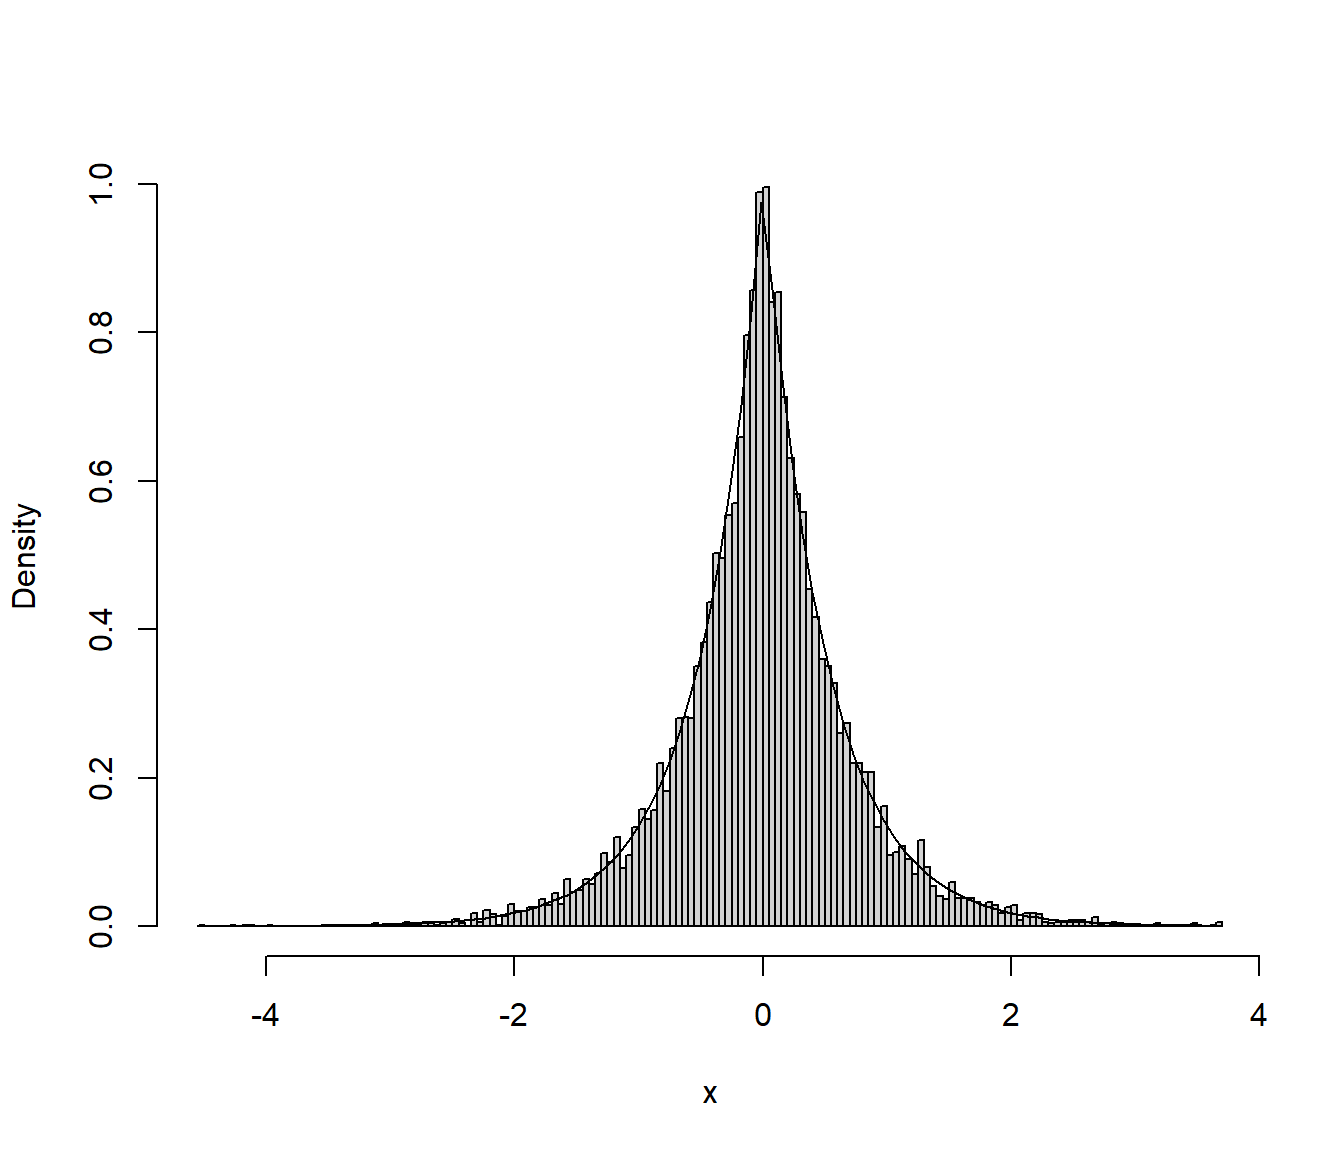
\includegraphics[width=0.7\linewidth]{05-Metodos_generales_continuas_files/figure-latex/dexp-inv-1} 

  }

  \caption{Distribución de los valores generados de una doble exponencial mediante el método de inversión.}\label{fig:dexp-inv}
  \end{figure}

  Como se trata de un método exacto de simulación, si está bien implementado, la distribución de los valores generados debería comportarse como una muestra genuina de la distribución objetivo.
\end{enumerate}

\hypertarget{ventajas-e-inconvenientes}{%
\subsection{Ventajas e inconvenientes}\label{ventajas-e-inconvenientes}}

Ventajas:

\begin{itemize}
\tightlist
\item
  Aplicable, en principio, a cualquier distribución continua.
\end{itemize}

Inconvenientes:

\begin{itemize}
\item
  Puede no ser posible encontrar una expresión explícita para
  \(F^{-1}\left( u\right).\)
\item
  Aún disponiendo de una expresión explícita para
  \(F^{-1}\left( u\right)\), su evaluación directa puede requerir
  mucho tiempo de computación.
\end{itemize}

Alternativas:

\begin{itemize}
\item
  Emplear métodos numéricos para resolver \(F(x) - u=0\)
  (requeriría resolver numéricamente esta ecuación para cada
  valor aleatorio que se desee generar).
\item
  Utilizar una aproximación a \(F^{-1}\left( u\right)\)
  (inversión aproximada).
\end{itemize}

\hypertarget{inversiuxf3n-aproximada}{%
\subsection{Inversión aproximada}\label{inversiuxf3n-aproximada}}

En muchos casos en los que no se puede emplear la expresión exacta de la función
cuantil \(F^{-1}\left( u\right)\), se dispone de una aproximación suficientemente
buena que se puede emplear en el algoritmo anterior (se obtendrían simulaciones
con una distribución aproximada a la deseada).

Por ejemplo, para aproximar la función cuantil de la normal estándar,
Odeh y Evans (1974) consideraron la siguiente función auxiliar\footnote{R emplea una aproximación similar, basada en el algoritmo de Wichura (1988) más preciso, y que está implementado en el fichero fuente \href{https://svn.r-project.org/R/trunk/src/nmath/qnorm.c}{qnorm.c}.}:
\[ g\left( v\right)  =\sqrt{-2\ln v}\frac{A\left( \sqrt{-2\ln v}\right)
}{B\left( \sqrt{-2\ln v}\right)  },\]
siendo \(A(x) =\sum_{i=0}^{4}a_{i}x^{i}\)
y \(B(x) =\sum_{i=0}^{4}b_{i}x^{i}\) con:

\[\begin{array}{ll}
a_{0}=-0.322232431088 &  b_{0}=0.0993484626060 \\
a_{1}=-1 &  b_{1}=0.588581570495 \\
a_{2}=-0.342242088547 & b_{2}=0.531103462366 \\
a_{3}=-0.0204231210245 & b_{3}=0.103537752850 \\
a_{4}=-0.0000453642210148 & b_{4}=0.0038560700634
\end{array}\]

La aproximación consiste en utilizar \(g\left( 1-u\right)\) en lugar de
\(F^{-1}\left( u\right)\) para los valores de \(u\in[10^{-20},\frac12]\)
y \(-g\left( u\right)\) si \(u\in[\frac12,1-10^{-20}]\). Para \(u\notin [10^{-20},1-10^{-20}]\) (que sólo ocurre con una probabilidad de
\(2\cdot10^{-20}\)) la aproximación no es recomendable.

\begin{conjecture}[de Odeh y Evans]
\protect\hypertarget{cnj:Odeh-Evans}{}{\label{cnj:Odeh-Evans} \iffalse (de Odeh y Evans) \fi{} }

\begin{enumerate}
\def\labelenumi{\arabic{enumi}.}
\item
  Generar \(U \sim U(0, 1)\).
\item
  Si \(U<10^{-20}\) ó \(U>1-10^{-20}\) entonces volver a 1.
\item
  Si \(U<0.5\) entonces hacer \(X=g\left(1-U\right)\)
  en caso contrario hacer \(X=-g\left( U\right)\).
\item
  Devolver \(X\).
\end{enumerate}
\end{conjecture}

En manuales de funciones matemáticas, como \href{https://www.math.ubc.ca/~cbm/aands/frameindex.htm}{Abramowitz y Stegun (1964)},
se tienen aproximaciones de la función cuantil de las principales distribuciones
(por ejemplo en la página \href{https://www.math.ubc.ca/~cbm/aands/page_933.htm}{993}
las correspondientes a la normal estándar).

\hypertarget{AR}{%
\section{Método de aceptación rechazo}\label{AR}}

Se trata de un método universal alternativo al de inversión para
el caso de que no se pueda emplear la función cuantil,
pero se dispone de una expresión (preferiblemente sencilla) para la
función de densidad \(f\left( x \right)\).

Si \(f\) es la densidad objetivo, la idea es simular una variable aleatoria
bidimensional \(\left( X, Y\right)\) con distribución
uniforme en el hipografo de \(f\) (el conjunto de puntos del plano
comprendidos entre el eje OX y \(f\)):
\[A_{f}=\left\{ \left( x,y\right) \in \mathbb{R}^{2}:0\leq y\leq
f(x) \right\}.\]
De esta forma la primera componente tendrá la distribución deseada:

\begin{center}\includegraphics[width=0.7\linewidth]{images/rechazo} \end{center}

\[ P\left( a<X<b\right) = \frac{\text{Area de }\left\{ \left( x,y\right) \in 
\mathbb{R}^{2}:a<x<b;~0\leq y\leq f(x) \right\} }{\text{Area de }
A_{f}} \\
= \int_{a}^{b}f(x) dx \]

El resultado anterior es también válido para una cuasi-densidad \(f^{\ast}\)
(no depende de la constante normalizadora).
El resultado general sería en siguiente:

\begin{itemize}
\item
  Si \(X\) es una variable aleatoria con función de densidad \(f\)
  y \(U \sim \mathcal{U}(0, 1)\) entonces
  \[\left( X,c\cdot U\cdot f(x) \right) \sim \mathcal{U}\left(
  A_{cf}\right)\]
  siendo
  \(A_{cf}=\left\{ \left( x, y \right) \in \mathbb{R}^{2} : 0 \leq y \leq cf\left( x \right) \right\}\).
\item
  Recíprocamente si \(\left( X,Y\right) \sim \mathcal{U}\left(A_{cf}\right)\) entonces\footnote{Emplearemos también \(X\sim f\) para indicar que \(X\) es una variable aleatoria con función de densidad \(f\).} \(X\sim f\).
\end{itemize}

Para generar valores de una variable aleatoria bidimensional con distribución uniforme
en \(A_{f}\) (o en \(A_{f^{\ast }}\)), se emplea el resultado anterior para
generar valores en \(A_{cg} \supset A_{f}\), siendo \(g\) una densidad auxiliar
(preferiblemente fácil de simular y similar a \(f\)).
Teniendo en cuenta además que:

\begin{itemize}
\tightlist
\item
  Si \(\left( X,Y\right) \sim \mathcal{U}\left( A\right)\) y
  \(B \subset A\Rightarrow \left. \left( X,Y\right) \right\vert _{B} \sim \mathcal{U}\left(B\right)\)
\end{itemize}

Por tanto, si \(\left( T, Y \right)\) sigue una distribución
uniforme en \(A_{cg}\), aceptando los valores de
\(\left( T, Y\right)\) que pertenezcan a \(A_{f}\) (o a \(A_{f^{\ast }}\)) se obtendrán
generaciones con distribución uniforme sobre \(A_{f}\) (o \(A_{f^{\ast }}\))
y la densidad de la primera componente \(T\) será \(f\).

\hypertarget{algoritmo}{%
\subsection{Algoritmo}\label{algoritmo}}

Supongamos que \(f\) es la densidad objetivo y \(g\) es una densidad
auxiliar (fácil de simular y similar a \(f\)), de forma que
existe una constante \(c>0\) tal que:
\[f(x) \leq c\cdot g(x) 
\text{, }\forall x\in \mathbb{R}\text{.}\]

\begin{conjecture}[Método de aceptación-rechazo; Von Neuman, 1951]
\protect\hypertarget{cnj:aceptacion-rechazo}{}{\label{cnj:aceptacion-rechazo} \iffalse (Método de aceptación-rechazo; Von Neuman, 1951) \fi{} }

\begin{enumerate}
\def\labelenumi{\arabic{enumi}.}
\item
  Generar \(U \sim \mathcal{U}(0, 1)\).
\item
  Generar \(T\sim g\).
\item
  Si \(c\cdot U\cdot g\left( T\right) \leq f\left( T\right)\)
  devolver \(X=T\),

  en caso contrario volver al paso 1.
\end{enumerate}
\end{conjecture}

\hypertarget{densidades-acotadas-en-un-intervalo-cerrado}{%
\subsection{Densidades acotadas en un intervalo cerrado}\label{densidades-acotadas-en-un-intervalo-cerrado}}

Sea \(f\) una función de densidad cualquiera con soporte en un intervalo cerrado \([a,b]\) (es decir, \(\{x : f(x) > 0\}=[a,b]\)) de tal forma que existe una constante \(M>0\) tal que \(f(x) \leq M\) \(\forall x\) (es decir, \(f\) es acotada superiormente).
En este caso puede tomarse como densidad auxiliar \(g\), la de una \(\mathcal{U}(a,b)\).
En efecto, tomando \(c = M\left( b-a\right)\) y teniendo en cuenta que
\[g(x) = \left\{
\begin{array}{ll}\frac{1}{b-a} & \text{si } x \in [a,b]\\
0 & \text{en caso contrario}
\end{array} \right.\]
se tiene que \(f(x) \leq M = \frac{c}{b-a}=c \cdot g(x)\),
\(\forall x \in [a,b]\).
Así pues, el algoritmo quedaría como sigue:

\begin{enumerate}
\def\labelenumi{\arabic{enumi}.}
\item
  Generar \(U,V\sim \mathcal{U}(0, 1)\).
\item
  Hacer \(T = a + \left( b-a \right) V\).
\item
  Si \(M \cdot U\leq f\left( T \right)\)
  devolver \(X = T\),

  en caso contrario volver al paso 1.
\end{enumerate}

\textbf{Nota}: no confundir \(M\) con \(c = M \left( b - a \right)\).

\begin{exercise}[Simulación de la normal mediante la doble exponencial]
\protect\hypertarget{exr:dnorm-ddexp-ar}{}{\label{exr:dnorm-ddexp-ar} \iffalse (Simulación de la normal mediante la doble exponencial) \fi{} }
\end{exercise}

Desarrollar el código necesario para generar, por el método de
aceptación-rechazo, una muestra de \(n\) observaciones de una
distribución normal estándar:
\[f(x)  =\frac{1}{\sqrt{2\pi}}e^{-\frac{x^{2}}{2}}\text{, }x\in\mathbb{R}\text{, }\]
empleando como distribución auxiliar una doble exponencial con \(\lambda=1\)
(más adelante veremos que esta es la elección óptima para el parámetro de la densidad auxiliar) y que la cota óptima es:
\[c_{\text{opt}}=\sqrt{\frac{2e}{\pi}} \approx 1.3155\]
Para establecer la condición de aceptación o rechazo se puede tener en cuenta que:
\[c\cdot U\cdot\frac{g\left( T\right)  }{f\left( T\right)  }=\sqrt{\frac
{2e}{\pi}}U\sqrt{\frac{\pi}{2}}\exp\left( \frac{T^{2}}{2}-\left\vert
T\right\vert \right)  =U\cdot\exp\left( \frac{T^{2}}{2}-\left\vert
T\right\vert +\frac{1}{2}\right) ,\]
aunque en general puede ser recomendable emplear
\(c\cdot U\cdot g\left( T\right) \leq f\left( T\right)\).

En el código del Ejercicio \ref{exr:ddexp} se definió la densidad auxiliar \texttt{ddexp(x,\ lambda)} y la función \texttt{rdexp(lambda)} para generar un valor aleatorio de esta densidad.
Si comparamos la densidad objetivo con la auxiliar reescalada con los parámetros óptimos (Figura \ref{fig:dnorm-ddexp-plot}), vemos que esta última está por encima, como debería ocurrir, pero llegan a tocarse (se está empleando la cota óptima; ver siguiente sección).

\begin{Shaded}
\begin{Highlighting}[]
\CommentTok{# densidad objetivo: dnorm}
\CommentTok{# densidad auxiliar: ddexp}
\NormalTok{c.opt <-}\StringTok{ }\KeywordTok{sqrt}\NormalTok{(}\DecValTok{2}\OperatorTok{*}\KeywordTok{exp}\NormalTok{(}\DecValTok{1}\NormalTok{)}\OperatorTok{/}\NormalTok{pi)}
\NormalTok{lambda.opt <-}\StringTok{ }\DecValTok{1}
\KeywordTok{curve}\NormalTok{(c.opt }\OperatorTok{*}\StringTok{ }\KeywordTok{ddexp}\NormalTok{(x), }\DataTypeTok{xlim =} \KeywordTok{c}\NormalTok{(}\OperatorTok{-}\DecValTok{4}\NormalTok{, }\DecValTok{4}\NormalTok{), }\DataTypeTok{lty =} \DecValTok{2}\NormalTok{)}
\KeywordTok{curve}\NormalTok{(}\KeywordTok{dnorm}\NormalTok{(x), }\DataTypeTok{add =} \OtherTok{TRUE}\NormalTok{)}
\end{Highlighting}
\end{Shaded}

\begin{figure}[!htb]

{\centering 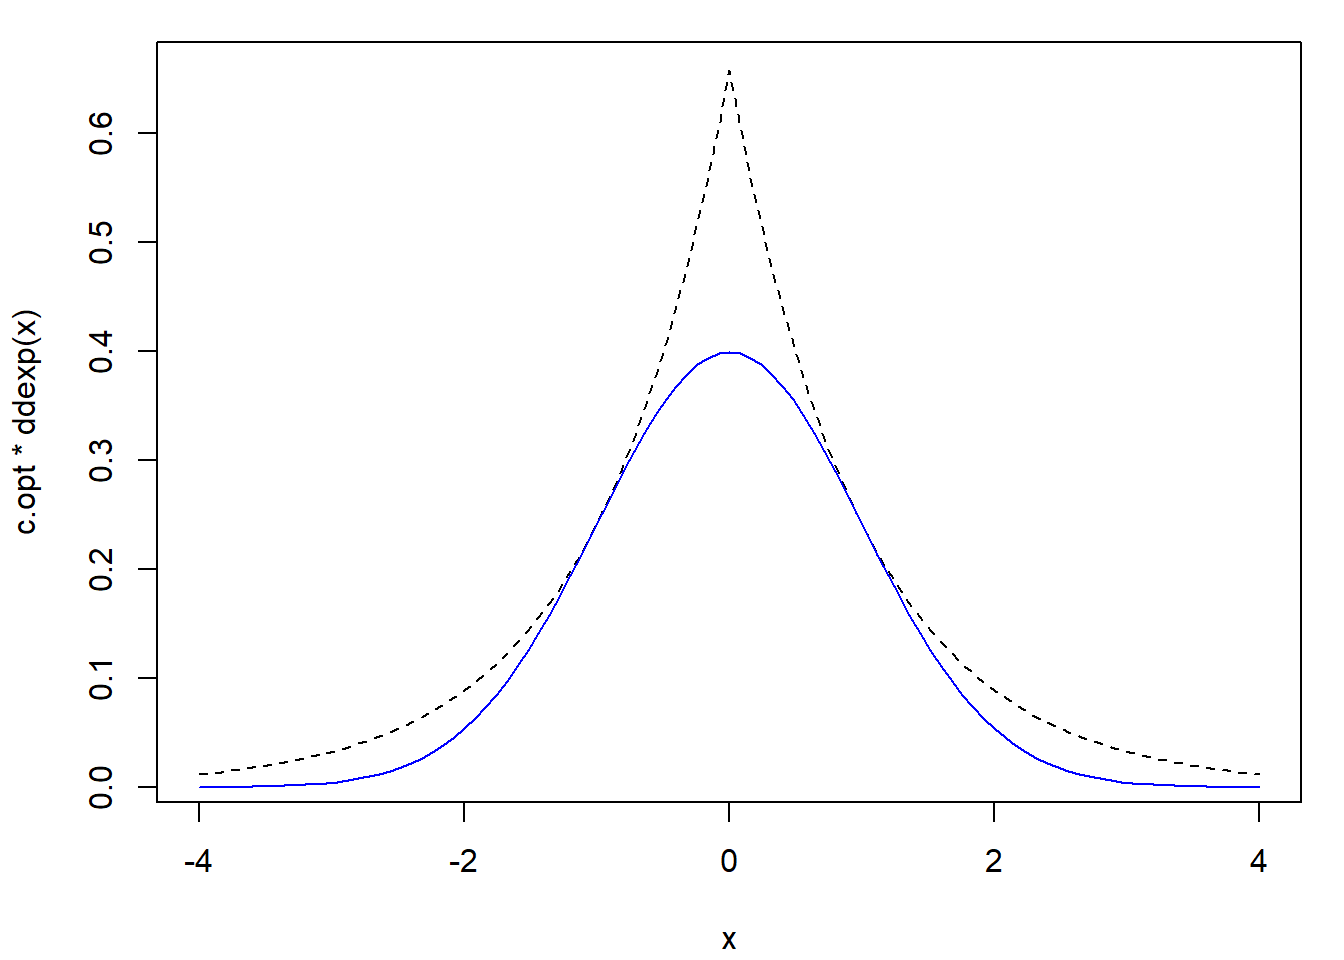
\includegraphics[width=0.7\linewidth]{05-Metodos_generales_continuas_files/figure-latex/dnorm-ddexp-plot-1} 

}

\caption{Densidad objetivo (normal estándar) y densidad auxiliar (doble exponencial) reescalada.}\label{fig:dnorm-ddexp-plot}
\end{figure}

Para generar los valores de la densidad objetivo podríamos emplear el siguiente código:

\begin{Shaded}
\begin{Highlighting}[]
\NormalTok{ngen <-}\StringTok{ }\DecValTok{0}

\NormalTok{rnormAR <-}\StringTok{ }\ControlFlowTok{function}\NormalTok{() \{}
\CommentTok{# Simulación por aceptación-rechazo}
\CommentTok{# Normal estandar a partir de doble exponencial}
  \ControlFlowTok{while}\NormalTok{ (}\OtherTok{TRUE}\NormalTok{) \{}
\NormalTok{    U <-}\StringTok{ }\KeywordTok{runif}\NormalTok{(}\DecValTok{1}\NormalTok{)}
\NormalTok{    X <-}\StringTok{ }\KeywordTok{rdexp}\NormalTok{(lambda.opt) }\CommentTok{# rdexpn(1, lambda.opt)}
\NormalTok{    ngen <<-}\StringTok{ }\NormalTok{ngen }\OperatorTok{+}\StringTok{ }\DecValTok{1} \CommentTok{# Comentar esta línea para uso normal}
    \CommentTok{# if (U*exp((X^2+1)*0.5-abs(X)) <= 1) return(X)}
    \ControlFlowTok{if}\NormalTok{ (c.opt }\OperatorTok{*}\StringTok{ }\NormalTok{U }\OperatorTok{*}\StringTok{ }\KeywordTok{ddexp}\NormalTok{(X, lambda.opt) }\OperatorTok{<=}\StringTok{ }\KeywordTok{dnorm}\NormalTok{(X)) }\KeywordTok{return}\NormalTok{(X)}
\NormalTok{  \}}
\NormalTok{\}}

\NormalTok{rnormARn <-}\StringTok{ }\ControlFlowTok{function}\NormalTok{(}\DataTypeTok{n =} \DecValTok{1000}\NormalTok{) \{}
\CommentTok{# Simulación n valores N(0,1)}
\NormalTok{    x <-}\StringTok{ }\KeywordTok{numeric}\NormalTok{(n)}
    \ControlFlowTok{for}\NormalTok{(i }\ControlFlowTok{in} \DecValTok{1}\OperatorTok{:}\NormalTok{n) x[i] <-}\StringTok{ }\KeywordTok{rnormAR}\NormalTok{()}
    \KeywordTok{return}\NormalTok{(x)}
\NormalTok{\}}

\CommentTok{# Grafico}
\end{Highlighting}
\end{Shaded}

\begin{enumerate}
\def\labelenumi{\alph{enumi})}
\item
  Generar una muestra de \(10^{4}\) observaciones empleando este
  algoritmo. Obtener el tiempo de CPU y calcular el número medio
  de generaciones de la distribución auxiliar.

\begin{Shaded}
\begin{Highlighting}[]
\KeywordTok{set.seed}\NormalTok{(}\DecValTok{54321}\NormalTok{)}
\NormalTok{nsim <-}\StringTok{ }\DecValTok{10}\OperatorTok{^}\DecValTok{4}

\NormalTok{ngen <-}\StringTok{ }\DecValTok{0}
\KeywordTok{system.time}\NormalTok{(x <-}\StringTok{ }\KeywordTok{rnormARn}\NormalTok{(nsim))}
\end{Highlighting}
\end{Shaded}

\begin{verbatim}
##    user  system elapsed 
##    0.12    0.00    0.12
\end{verbatim}

\begin{Shaded}
\begin{Highlighting}[]
\CommentTok{# Nº generaciones}
\NormalTok{\{}
\KeywordTok{cat}\NormalTok{(}\StringTok{"}\CharTok{\textbackslash{}n}\StringTok{Número de generaciones = "}\NormalTok{, ngen)}
\KeywordTok{cat}\NormalTok{(}\StringTok{"}\CharTok{\textbackslash{}n}\StringTok{Número medio de generaciones = "}\NormalTok{, ngen}\OperatorTok{/}\NormalTok{nsim)}
\KeywordTok{cat}\NormalTok{(}\StringTok{"}\CharTok{\textbackslash{}n}\StringTok{Proporción de rechazos = "}\NormalTok{, }\DecValTok{1}\OperatorTok{-}\NormalTok{nsim}\OperatorTok{/}\NormalTok{ngen, }\StringTok{"}\CharTok{\textbackslash{}n}\StringTok{"}\NormalTok{)}
\NormalTok{\}}
\end{Highlighting}
\end{Shaded}

\begin{verbatim}
## 
## Número de generaciones =  13163
## Número medio de generaciones =  1.3163
## Proporción de rechazos =  0.2402948
\end{verbatim}
\item
  Representar el histograma y compararlo con la densidad teórica.

\begin{Shaded}
\begin{Highlighting}[]
\KeywordTok{hist}\NormalTok{(x, }\DataTypeTok{breaks =} \StringTok{"FD"}\NormalTok{, }\DataTypeTok{freq =} \OtherTok{FALSE}\NormalTok{)}
\KeywordTok{curve}\NormalTok{(dnorm, }\DataTypeTok{add =} \OtherTok{TRUE}\NormalTok{)}
\end{Highlighting}
\end{Shaded}

  \begin{figure}[!htb]

  {\centering 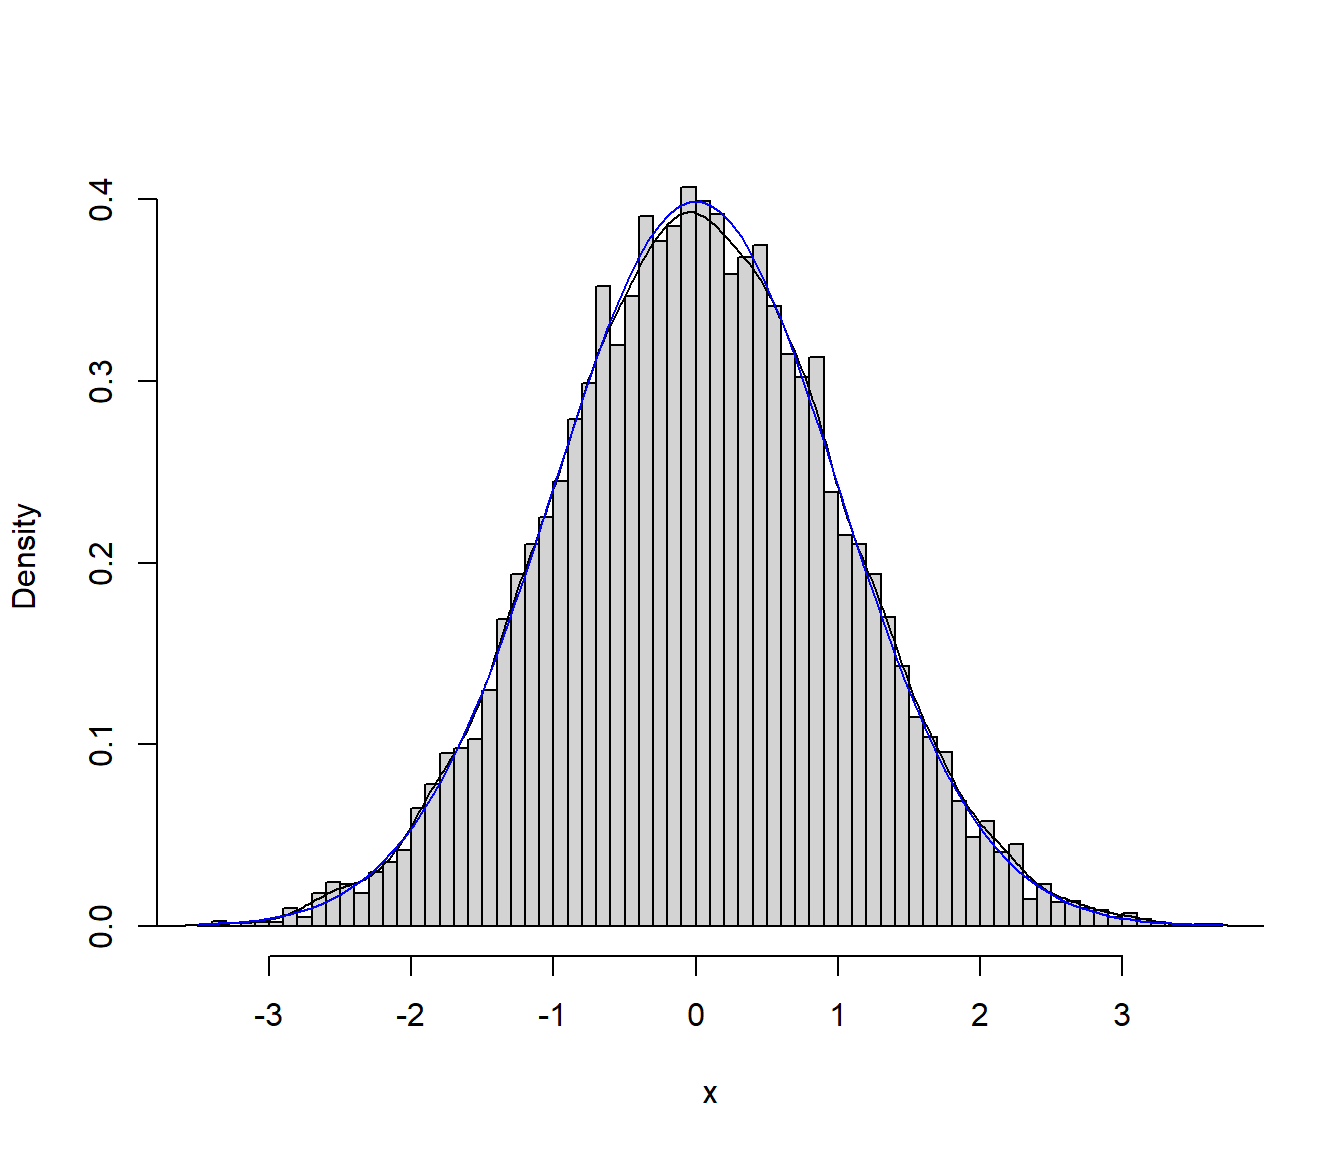
\includegraphics[width=0.7\linewidth]{05-Metodos_generales_continuas_files/figure-latex/dnorm-ar-1} 

  }

  \caption{Distribución de los valores generados mediante el método de aceptación-rechazo.}\label{fig:dnorm-ar}
  \end{figure}

  Podemos observar que la distribución de los valores generados es la que cabría esperar de una muestra de tamaño \texttt{nsim} de la distribución objetivo (lo que nos ayudaría a confirmar que el algoritmo está bien implementado, al ser un método exacto de simulación).
\end{enumerate}

\hypertarget{eficiencia-del-algoritmo}{%
\subsection{Eficiencia del algoritmo}\label{eficiencia-del-algoritmo}}

Como medida de la eficiencia del algoritmo de aceptación-rechazo
podríamos considerar el número de iteraciones del algoritmo,
es decir, el número de generaciones de la densidad auxiliar y
de comparaciones para aceptar un valor de la densidad objetivo.
Este número \(N\) es aleatorio y sigue una distribución geométrica
(número de pruebas necesarias hasta obtener el primer éxito)
con parámetro \(p\) (probabilidad de éxito) la probabilidad de aceptación
en el paso 3:
\[p = \frac{\text{area}\left(
        A_{f}\right) }{\text{area}\left( A_{cg}\right) }=\frac{1}{c}.\]
Por tanto:
\[E\left( N \right) = \frac1p = c\]
es el número medio de iteraciones del algoritmo
(el número medio de pares de variables \(\left( T,U\right)\)
que se necesitan generar, y de comparaciones, para obtener
una simulación de la densidad objetivo).

Es obvio, por tanto, que cuanto más cercano a 1 sea el valor de \(c\) más eficiente será el algoritmo (el caso de \(c=1\) se correspondería con \(g=f\) y no tendría sentido emplear este algoritmo).
El principal problema con este método es encontrar una densidad auxiliar \(g\) de forma que:
\[c_{\text{opt}}=\max_{\{x : g(x) >0\}}
\frac{f(x) }{g(x) }.\]
sea próximo a 1.
Una solución intermedia consiste en seleccionar una familia paramétrica de densidades \(\{g_{\theta} : \theta \in \Theta\}\) entre las que haya alguna que se parezca bastante a \(f\),
encontrar el valor de \(c\) óptimo para cada densidad de esa familia:
\[c_{\theta}=\max_{x}\frac{f\left(  x\right)  }{g_{\theta}(x) }\]
y, finalmente, elegir el mejor valor \(\theta_{0}\) del parámetro, en el sentido de ofrecer el menor posible \(c_{\theta}\):
\[c_{\theta_{0}}=\min_{\theta\in\Theta}\max_{x}\frac{f\left(  x\right) }{g_{\theta}\left(  x\right)  }.\]

\begin{exercise}[Simulación de la normal mediante la doble exponencial, continuación]
\protect\hypertarget{exr:dnorm-ddexp-arb}{}{\label{exr:dnorm-ddexp-arb} \iffalse (Simulación de la normal mediante la doble exponencial, continuación) \fi{} }
\end{exercise}

Continuando con el Ejercicio \ref{exr:dnorm-ddexp-ar} anterior del método de aceptación-rechazo para generar observaciones de una distribución normal estándar, empleando como distribución auxiliar una doble exponencial:

\begin{enumerate}
\def\labelenumi{\alph{enumi})}
\setcounter{enumi}{2}
\item
  Aproximar la cota óptima numéricamente.

\begin{Shaded}
\begin{Highlighting}[]
\CommentTok{# NOTA: Cuidado con los límites}
\CommentTok{# optimize(f=function(x) dnorm(x)/ddexp(x), maximum=TRUE, interval=c(-0.5,0.5))}
\KeywordTok{optimize}\NormalTok{(}\DataTypeTok{f =} \ControlFlowTok{function}\NormalTok{(x) }\KeywordTok{dnorm}\NormalTok{(x)}\OperatorTok{/}\KeywordTok{ddexp}\NormalTok{(x), }\DataTypeTok{maximum =} \OtherTok{TRUE}\NormalTok{, }\DataTypeTok{interval =} \KeywordTok{c}\NormalTok{(}\DecValTok{0}\NormalTok{, }\DecValTok{2}\NormalTok{))}
\end{Highlighting}
\end{Shaded}

\begin{verbatim}
## $maximum
## [1] 1
## 
## $objective
## [1] 1.315489
\end{verbatim}

  Vemos que la aproximación numérica coincide con el valor óptimo real \(c_{\text{opt}}=\sqrt{\frac{2e}{\pi}} \approx\) 1.3154892 (que se alcanza en \(x = \pm 1\)).
\item
  Aproximar el parámetro óptimo de la densidad auxiliar
  numéricamente (normalmente comenzaríamos por este paso).

\begin{Shaded}
\begin{Highlighting}[]
\CommentTok{# Obtención de valores c y lambda óptimos aproximados}
\NormalTok{fopt <-}\StringTok{ }\ControlFlowTok{function}\NormalTok{(lambda) \{}
  \CommentTok{# Obtiene c fijado lambda}
  \KeywordTok{optimize}\NormalTok{(}\DataTypeTok{f =} \ControlFlowTok{function}\NormalTok{(x) }\KeywordTok{dnorm}\NormalTok{(x)}\OperatorTok{/}\KeywordTok{ddexp}\NormalTok{(x,lambda),}
           \DataTypeTok{maximum =} \OtherTok{TRUE}\NormalTok{, }\DataTypeTok{interval =} \KeywordTok{c}\NormalTok{(}\DecValTok{0}\NormalTok{, }\DecValTok{2}\NormalTok{))}\OperatorTok{$}\NormalTok{objective}
\NormalTok{\}}

\CommentTok{# Encontrar lambda que minimiza}
\NormalTok{res <-}\StringTok{ }\KeywordTok{optimize}\NormalTok{(fopt, }\DataTypeTok{interval =} \KeywordTok{c}\NormalTok{(}\FloatTok{0.5}\NormalTok{, }\DecValTok{2}\NormalTok{))}
\NormalTok{lambda.opt2 <-}\StringTok{ }\NormalTok{res}\OperatorTok{$}\NormalTok{minimum}
\NormalTok{c.opt2 <-}\StringTok{ }\NormalTok{res}\OperatorTok{$}\NormalTok{objective}
\end{Highlighting}
\end{Shaded}
\end{enumerate}

\hypertarget{ejemplo-inferencia-bayesiana}{%
\subsection{Ejemplo: Inferencia Bayesiana}\label{ejemplo-inferencia-bayesiana}}

El algoritmo de Aceptación-Rechazo se emplea habitualmente en
Inferencia Bayesiana:

\begin{itemize}
\item
  \(f(x|\theta )\) densidad muestral.
\item
  \(\pi (\theta )\) densidad a priori.
\item
  \(\mathbf{x}=(x_{1},...,x_n)^{\prime }\) muestra observada.
\item
  La distribución a posteriori de \(\theta\) es:
  \[\pi (\theta |\mathbf{x})=\frac{L(\mathbf{x}|\theta )\pi (\theta )}
  {\int L(\mathbf{x}|\theta )\pi (\theta )d\theta }\]
  siendo \(L(\mathbf{x}|\theta )\) la función de verosimilitud
  (\(L(\mathbf{x}|\theta )=\prod\limits_{i=1}^{n}f(x_{i}|\theta)\)
  suponiendo i.i.d.). Es decir:
  \[\pi (\theta |\mathbf{x})\propto L(\mathbf{x}|\theta )\pi (\theta ).\]
\end{itemize}

Para simular valores de la densidad a posteriori \(\pi (\theta | \mathbf{x})\)
a partir de la densidad a priori \(\pi (\theta )\)

\begin{itemize}
\item
  \(\pi (\theta |\mathbf{x})/\pi (\theta )\propto L(\mathbf{x}|\theta )\)
\item
  \(L(\mathbf{x}|\theta )\leq c^{\prime }=L(\mathbf{x}|\hat{\theta})\) siendo
  \(\hat{\theta}\) el estimador MV de \(\theta\).
\end{itemize}

Algoritmo:

\begin{enumerate}
\def\labelenumi{\arabic{enumi}.}
\item
  Generar \(U \sim \mathcal{U}(0, 1)\).
\item
  Generar \(\tilde{\theta}\sim \pi (\theta )\).
\item
  Si \(L(\mathbf{x}|\hat{\theta})\cdot U \leq L(\mathbf{x}|\tilde{\theta})\) devolver \(\tilde{\theta}\),

  en caso contrario volver al paso 1.
\end{enumerate}

\begin{exercise}[Simulación de la distribución a posteriori a partir de la distribución a priori]
\protect\hypertarget{exr:post-pri-ar}{}{\label{exr:post-pri-ar} \iffalse (Simulación de la distribución a posteriori a partir de la distribución a priori) \fi{} }
\end{exercise}

Para la estimación Bayes de la media de una normal se suele utilizar
como distribución a priori una Cauchy.

\begin{enumerate}
\def\labelenumi{\alph{enumi})}
\item
  Generar una muestra i.i.d. \(X_{i}\sim N(\theta_{0},1)\) de tamaño
  \(n=10\) con \(\theta_{0}=1\). Utilizar una \(Cauchy(0,1)\)
  (\texttt{rcauchy}) como distribución a priori y como densidad auxiliar
  para simular por aceptación-rechazo una muestra de la densidad a
  posteriori (emplear \texttt{dnorm} para construir la verosimilitud).
  Obtener el intervalo de probabilidad/credibilidad al 95\%.

\begin{Shaded}
\begin{Highlighting}[]
\NormalTok{mu0 <-}\StringTok{ }\DecValTok{1}
\NormalTok{n <-}\StringTok{ }\DecValTok{10}
\NormalTok{nsim <-}\StringTok{ }\DecValTok{10}\OperatorTok{^}\DecValTok{3}
\KeywordTok{set.seed}\NormalTok{(}\DecValTok{54321}\NormalTok{)}
\NormalTok{x <-}\StringTok{ }\KeywordTok{rnorm}\NormalTok{(n, }\DataTypeTok{mean =}\NormalTok{ mu0)}

\CommentTok{# Función de verosimilitud}
\NormalTok{lik <-}\StringTok{ }\ControlFlowTok{function}\NormalTok{(mu)\{}\KeywordTok{prod}\NormalTok{(}\KeywordTok{dnorm}\NormalTok{(x, }\DataTypeTok{mean =}\NormalTok{ mu))\}}

\CommentTok{# Cota óptima}
\CommentTok{# Estimación por máxima verosimilitud}
\NormalTok{emv <-}\StringTok{ }\KeywordTok{optimize}\NormalTok{(}\DataTypeTok{f =}\NormalTok{ lik, }\DataTypeTok{int =} \KeywordTok{range}\NormalTok{(x), }\DataTypeTok{maximum =} \OtherTok{TRUE}\NormalTok{)}
\NormalTok{emv}
\end{Highlighting}
\end{Shaded}

\begin{verbatim}
## $maximum
## [1] 0.7353805
## 
## $objective
## [1] 3.303574e-08
\end{verbatim}

\begin{Shaded}
\begin{Highlighting}[]
\NormalTok{c <-}\StringTok{ }\NormalTok{emv}\OperatorTok{$}\NormalTok{objective}
\end{Highlighting}
\end{Shaded}

  En este caso concreto, ya sabríamos que el estimador máximo verosímil es la media muestral:

\begin{Shaded}
\begin{Highlighting}[]
\KeywordTok{mean}\NormalTok{(x)}
\end{Highlighting}
\end{Shaded}

\begin{verbatim}
## [1] 0.7353958
\end{verbatim}

  y por tanto:

\begin{Shaded}
\begin{Highlighting}[]
\NormalTok{c <-}\StringTok{ }\KeywordTok{lik}\NormalTok{(}\KeywordTok{mean}\NormalTok{(x))}
\NormalTok{c    }
\end{Highlighting}
\end{Shaded}

\begin{verbatim}
## [1] 3.303574e-08
\end{verbatim}

  Finalmente podríamos emplear el siguiente código para generar simulaciones de la distribución a posteriori mediante aceptación-rechazo a partir de la distribución de Cauchy:

\begin{Shaded}
\begin{Highlighting}[]
\NormalTok{ngen <-}\StringTok{ }\NormalTok{nsim}
\NormalTok{Y <-}\StringTok{ }\KeywordTok{rcauchy}\NormalTok{(nsim)}
\NormalTok{ind <-}\StringTok{ }\NormalTok{(c}\OperatorTok{*}\KeywordTok{runif}\NormalTok{(nsim) }\OperatorTok{>}\StringTok{ }\KeywordTok{sapply}\NormalTok{(Y, lik)) }\CommentTok{# TRUE si no verifica condición}
\CommentTok{# Volver a generar si no verifica condición}
\ControlFlowTok{while}\NormalTok{ (}\KeywordTok{sum}\NormalTok{(ind)}\OperatorTok{>}\DecValTok{0}\NormalTok{)\{}
\NormalTok{  le <-}\StringTok{ }\KeywordTok{sum}\NormalTok{(ind)}
\NormalTok{  ngen <-}\StringTok{ }\NormalTok{ngen }\OperatorTok{+}\StringTok{ }\NormalTok{le}
\NormalTok{  Y[ind] <-}\StringTok{ }\KeywordTok{rcauchy}\NormalTok{(le)}
\NormalTok{  ind[ind] <-}\StringTok{ }\NormalTok{(c}\OperatorTok{*}\KeywordTok{runif}\NormalTok{(le) }\OperatorTok{>}\StringTok{ }\KeywordTok{sapply}\NormalTok{(Y[ind], lik)) }\CommentTok{# TRUE si no verifica condición}
\NormalTok{\}}

\NormalTok{\{ }\CommentTok{# Número generaciones}
  \KeywordTok{cat}\NormalTok{(}\StringTok{"Número de generaciones = "}\NormalTok{, ngen)}
  \KeywordTok{cat}\NormalTok{(}\StringTok{"}\CharTok{\textbackslash{}n}\StringTok{Número medio de generaciones = "}\NormalTok{, ngen}\OperatorTok{/}\NormalTok{nsim)}
  \KeywordTok{cat}\NormalTok{(}\StringTok{"}\CharTok{\textbackslash{}n}\StringTok{Proporción de rechazos = "}\NormalTok{, }\DecValTok{1}\OperatorTok{-}\NormalTok{nsim}\OperatorTok{/}\NormalTok{ngen,}\StringTok{"}\CharTok{\textbackslash{}n}\StringTok{"}\NormalTok{)}
\NormalTok{\}}
\end{Highlighting}
\end{Shaded}

\begin{verbatim}
## Número de generaciones =  5898
## Número medio de generaciones =  5.898
## Proporción de rechazos =  0.830451
\end{verbatim}

\begin{Shaded}
\begin{Highlighting}[]
\CommentTok{# Intervalo de probabilidad al 95% (IC Bayes)}
\NormalTok{q <-}\StringTok{ }\KeywordTok{quantile}\NormalTok{(Y, }\KeywordTok{c}\NormalTok{(}\FloatTok{0.025}\NormalTok{, }\FloatTok{0.975}\NormalTok{))}

\CommentTok{# Representar estimador e IC Bayes}
\KeywordTok{hist}\NormalTok{(Y, }\DataTypeTok{freq=}\OtherTok{FALSE}\NormalTok{, }\DataTypeTok{main=}\StringTok{"Distribución a posteriori"}\NormalTok{)}
\CommentTok{# abline(v = mean(x), lty = 3) # Estimación frecuentista}
\KeywordTok{abline}\NormalTok{(}\DataTypeTok{v =} \KeywordTok{mean}\NormalTok{(Y), }\DataTypeTok{lty =} \DecValTok{2}\NormalTok{, }\DataTypeTok{lwd =} \DecValTok{2}\NormalTok{)  }\CommentTok{# Estimación Bayesiana}
\KeywordTok{abline}\NormalTok{(}\DataTypeTok{v =}\NormalTok{ q, }\DataTypeTok{lty =} \DecValTok{2}\NormalTok{)}
\end{Highlighting}
\end{Shaded}

  \begin{center}\includegraphics[width=0.7\linewidth]{05-Metodos_generales_continuas_files/figure-latex/unnamed-chunk-12-1} \end{center}
\item
  Repetir el apartado anterior con \(n=100\).
\end{enumerate}

\hypertarget{modificaciones-del-muxe9todo-de-aceptaciuxf3n-rechazo}{%
\section{Modificaciones del método de aceptación rechazo}\label{modificaciones-del-muxe9todo-de-aceptaciuxf3n-rechazo}}

En el tiempo de computación influye:

\begin{itemize}
\item
  La proporción de aceptación (debería ser grande).
\item
  La dificultad de simular con la densidad auxiliar.
\item
  El tiempo necesario para hacer la comparación en el paso 4.
\end{itemize}

En ciertos casos el tiempo de computación necesario para evaluar \(f(x)\) puede ser alto.

Para evitar evaluaciones de la densidad se puede emplear una función ``squeeze'' (Marsaglia, 1977) que aproxime la densidad por abajo:
\[s(x)\leq f(x).\]

Algoritmo:

\begin{enumerate}
\def\labelenumi{\arabic{enumi}.}
\item
  Generar \(U \sim \mathcal{U}(0, 1)\) y \(T\sim g\).
\item
  Si \(c\cdot U\cdot g\left( T\right) \leq s\left( T\right)\) devolver \(X=T\),

  en caso contrario

  2.a. si \(c\cdot U\cdot g\left( T\right) \leq f\left( T\right)\)
  devolver \(X=T\),

  2.b. en caso contrario volver al paso 1.
\end{enumerate}

\begin{center}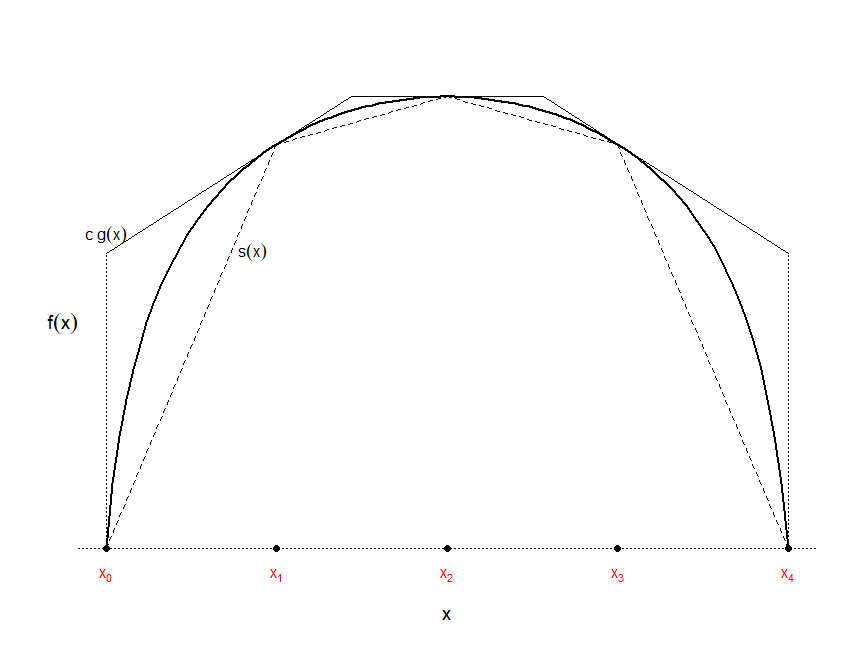
\includegraphics[width=0.7\linewidth]{images/squeeze} \end{center}

Cuanto mayor sea el área bajo \(s(x)\) (más próxima a 1)
más efectivo será el algoritmo.

Se han desarrollado métodos generales para la construcción de las
funciones \(g\) y \(s\) de forma automática
(cada vez que se evalúa la densidad se mejoran las aproximaciones).
Estos métodos se basan principalmente en que una transformación de
la densidad objetivo es cóncava o convexa.

\hypertarget{muestreo-por-rechazo-adaptativo-ars}{%
\subsection{Muestreo por rechazo adaptativo (ARS)}\label{muestreo-por-rechazo-adaptativo-ars}}

Supongamos que \(f\) es una cuasi-densidad log-cóncava
(i.e.~\(\frac{\partial ^{2}}{\partial x^{2}}\log f(x) <0, ~\forall x\)).

Sea \(S_n=\left\{ x_{i}:i=0,\cdots ,n+1\right\}\) con
\(f(x_{i})\) conocidos.

Denotamos por \(L_{i,i+1}(x)\) la recta pasando por \(\left( x_{i},\log f(x_{i})\right)\) y \(\left( x_{i+1},\log f(x_{i+1})\right)\)

\begin{itemize}
\item
  \(L_{i,i+1}(x)\leq \log f(x)\) en el intervalo
  \(I_{i}=(x_{i},x_{i+1}]\)
\item
  \(L_{i,i+1}(x)\geq \log f(x)\) fuera de \(I_{i}\)
\end{itemize}

En el intervalo \(I_{i}\) se definen las envolventes de \(\log f\left( x\right)\):

\begin{itemize}
\item
  \(\underline{\phi}_n(x)=L_{i,i+1}(x)\)
\item
  \(\overline{\phi}_n(x)=\min \left\{L_{i-1,i}(x),L_{i+1,i+2}(x)\right\}\)
\end{itemize}

Las envolventes de \(f(x)\) en \(I_{i}\) serán:

\begin{itemize}
\item
  \(s_n(x)=\exp \left( \underline{\phi}_n(x)\right)\)
\item
  \(G_n(x)=\exp \left( \overline{\phi}_n(x)\right)\)
\end{itemize}

Tenemos entonces que:
\[s_n(x)\leq f(x) \leq G_n(x)=c\cdot g_n(x)\]
donde \(g_n(x)\) es una mixtura discreta de distribuciones tipo exponencial truncadas
(las tasas pueden ser negativas),
que se puede simular fácilmente mediante el método de inversión.

Algoritmo (Gilks, 1992):

\begin{enumerate}
\def\labelenumi{\arabic{enumi}.}
\item
  Inizializar \(n\) y \(s_n\).
\item
  Generar \(U \sim \mathcal{U}(0, 1)\) y
  \(T\sim g_n\).
\item
  Si \(U\cdot G_n\left( T\right) \leq s_n\left( T\right)\)
  devolver \(X=T\),

  en caso contrario,

  3.a Si \(U\cdot G_n\left( T\right) \leq f\left( T\right)\)
  devolver \(X=T\).

  3.b Hacer \(n=n+1\), añadir \(T\) a \(S_n\)
  y actualizar \(s_n\) y \(G_n\).
\item
  Volver al paso 2.
\end{enumerate}

Gilks y Wild (1992) propusieron una ligera modificación empleando tangentes para construir la cota superior, de esta forma se obtiene un método más eficiente pero habrí que especificar la derivada de la densidad objetivo.

La mayoría de las densidades de la familia de distribuciones exponencial son log-cóncavas.
Hörmann (1995) extendió esta aproximación al caso de densidades \(T_{c}\)-cóncavas:
\[T_{c}(x) = signo(c)x^{c} \\
T_{0}(x) = \log (x).\]
Aparte de la transformación logarítmica, la transformación \(T_{-1/2}(x)=-1/\sqrt{x}\) es habitualmente la más empleada.

\hypertarget{muxe9todo-del-cociente-de-uniformes}{%
\subsection{Método del cociente de uniformes}\label{muxe9todo-del-cociente-de-uniformes}}

Se puede ver como una modificación del método de aceptación rechazo,
de especial interés cuando el soporte no es acotado.

Si \((U,V)\) se distribuye uniformemente sobre:
\[C_{h} = \left\{ \left( u,v\right) \in \mathbb{R}^{2} : 
0<u\leq \sqrt{h(v/u)} \right\},\]
siendo \(h\) una función no negativa integrable
(cuasi-densidad), entonces \(X=V/U\) tiene función de densidad
proporcional a \(h\) (Kinderman y Monahan, 1977).
Además \(C_{h}\) tiene área finita.

De modo análogo al método de aceptación-rechazo, hay modificaciones
para acelerar los cálculos y automatizar el proceso, construyendo
regiones mediante polígonos:\[C_{i}\subset C_{h}\subset C_{s}.\]

\hypertarget{composicion}{%
\section{Método de composición (o de simulación condicional)}\label{composicion}}

En ocasiones la densidad de interés se puede expresar como una
mixtura discreta de densidades:
\[f(x)=\sum_{j=1}^{k}p_{j}f_{j}(x)\]
con \(\sum_{j=1}^{k}p_j=1\), \(p_j\geq 0\) y \(f_j\) densidades
(sería también válido para funciones de distribución o variables aleatorias,
incluyendo el caso discreto).

Algoritmo:

\begin{enumerate}
\def\labelenumi{\arabic{enumi}.}
\item
  Generar \(J\) con distribución \(P\left( J=j \right) = p_j\).
\item
  Generar \(X\sim f_J\).
\end{enumerate}

\begin{example}[Distribución doble exponencial]
\protect\hypertarget{exm:dexp-mix}{}{\label{exm:dexp-mix} \iffalse (Distribución doble exponencial) \fi{} }
\end{example}
A partir de la densidad de la distribución doble exponencial:
\[f(x) =\frac{\lambda }{2}e^{-\lambda \left\vert x\right\vert }%
\text{, }\forall x\in \mathbb{R},\]
se deduce que:
\[f(x) =\frac{1}{2}f_{1}(x) +\frac{1}{2}f_{2}\left(
x\right)\]
siendo:
\[f_{1}(x) = \left\{ 
\begin{array}{ll}
\lambda e^{-\lambda x} & \text{si } x\geq 0 \\ 
0 & \text{si } x<0
\end{array}
\ \right. \\
f_{2}(x) = \left\{ 
\begin{array}{ll}
\lambda e^{\lambda x} & \text{si } x<0 \\ 
0 & \text{si } x\geq 0
\end{array}
\ \right.\]

El algoritmo resultante sería el siguiente (empleando dos números pseudo aleatorios uniformes, el primero para seleccionar el índice y el segundo para generar un valor de la correspondiente componente mediante el método de inversión):

\begin{enumerate}
\def\labelenumi{\arabic{enumi}.}
\item
  Generar \(U,V\sim \mathcal{U}(0, 1)\).
\item
  Si \(U<0.5\) devolver \(X=-\ln \left( 1-V\right)/\lambda\).
\item
  En caso contrario devolver \(X=\ln(V)/\lambda\).
\end{enumerate}

Observaciones:

\begin{itemize}
\item
  En ocasiones se hace un reciclado de los números aleatorios
  (solo se genera una uniforme, e.g.~\(V=2(U-0.5)\) si
  \(U\in (0.5,1)\)).
\item
  En ciertas ocasiones por comodidad, para simular una muestra de
  tamaño \(n\), se simulan muestras de tamaño \(np_{i}\) con densidad
  \(f_{i}\) y se combinan aleatoriamente.
\end{itemize}

Otro ejemplo de una mixtura discreta es el estimador tipo núcleo de la densidad (ver e.g.~la ayuda de la función \texttt{density()} de R o la \href{https://rubenfcasal.github.io/book_remuestreo/modunif-boot-suav.html}{Sección 3.3} del libro \href{https://rubenfcasal.github.io/book_remuestreo}{Técnicas de Remuestreo}).
Simular a partir de una estimación de este tipo es lo que se conoce como \emph{bootstrap suavizado}.

En el caso de una mixtura continua tendríamos:
\[f(x)=\int g(x|y)h(y)dy\]

Algoritmo:

\begin{enumerate}
\def\labelenumi{\arabic{enumi}.}
\item
  Generar \(Y\sim h\).
\item
  Generar \(X\sim g(\cdot |Y)\).
\end{enumerate}

Este algoritmo es muy empleado en Inferencia Bayesiana y en la simulación de algunas variables discretas (como la Binomial Negativa, denominada también distribución Gamma-Poisson, o la distribución Beta-Binomial; ver Sección \ref{notables-disc}),
ya que el resultado sería válido cambiando las funciones de densidad \(f\) y \(g\) por funciones de masa de probabilidad.

\hypertarget{notables-cont}{%
\section{Métodos específicos para la generación de algunas distribuciones notables}\label{notables-cont}}

En el pasado se ha realizado un esfuerzo considerable para desarrollar métodos eficientes para la simulación de las distribuciones de probabilidad más importantes.
Estos algoritmos se describen en la mayoría de los libros clásicos de simulación (e.g.~Cao, 2002, Capítulo 5)\footnote{Cuidado con la notación y la parametrización empleadas, puede variar entre referencias. Por ejemplo, en Cao (2002) la notación de la distribución Gamma es ligeramente distinta a la empleada en R y en el presente libro.}, principalmente porque resultaba necesario implementar estos métodos durante el desarrollo de software estadístico.
Hoy en día estos algoritmos están disponibles en numerosas bibliotecas y no es necesario su implementación (por ejemplo, se puede recurrir a R o emplear su librería matemática disponible en \url{https://svn.r-project.org/R/trunk/src/nmath}).
Sin embargo, además de que muchos de ellos servirían como ilustración de la aplicación de los métodos generales expuestos en secciones anteriores, pueden servir como punto de partida para la generación de otras distribuciones.

Entre los distintos métodos disponibles para la generación de las distribuciones continuas más conocidas podríamos destacar:

\begin{itemize}
\item
  Método de Box-Müller para la generación de normales independientes (pero que se puede generalizar para otras distribuciones y dependencia).
\item
  Algoritmos de Jöhnk (1963) y Cheng (1978) para la generación de la distribución Beta (como ejemplo de las eficiencias de los métodos de aceptación-rechazo).
\end{itemize}

\hypertarget{muxe9todo-de-box-muxfcller}{%
\subsection{Método de Box-Müller}\label{muxe9todo-de-box-muxfcller}}

Se basa en la siguiente propiedad. Dadas dos variables aleatorias independientes \(E \sim \exp\left( 1\right)\) y
\(U \sim \mathcal{U}( 0, 1 )\), las variables
\(\sqrt{2E} \cos 2\pi U\) y \(\sqrt{2E}\operatorname{sen} 2\pi U\) son
\(\mathcal{N}( 0, 1 )\) independientes.

\textbf{Algoritmo de Box-Müller}

\begin{enumerate}
\def\labelenumi{\arabic{enumi}.}
\item
  Generar \(U,V\sim \mathcal{U}( 0, 1 )\).
\item
  Hacer \(W_1=\sqrt{-2\ln U}\) y \(W_2=2\pi V\).
\item
  Devolver \(X_1=W_1\cos W_2\), \(X_2=W_1\operatorname{sen}W_2\).
\end{enumerate}

Podemos hacer que la función \texttt{rnorm()} de R emplee este algoritmo estableciendo el parámetro \texttt{normal.kind} a \texttt{"Box-Muller"} en una llamada previa a \texttt{set.seed()} o \texttt{RNGkind()}.

Este método está relacionado con el denominado \emph{método FFT} (transformada de Fourier; e.g.~Davies y Harte, 1987) para la generación de una normal multidimensional con dependencia, que resulta ser equivalente al \emph{Circular embedding} (Dietrich and Newsam, 1997).
La idea de estos métodos es que, considerando módulos exponenciales y fases uniformes generamos normales independientes, pero cambiando la varianza de los módulos (\(W_1\)) podemos inducir dependencia.
Adicionalmente, cambiando la distribución de las fases (\(W_2\)) se generan distribuciones distintas de la normal.

\hypertarget{discretas}{%
\chapter{Simulación de variables discretas}\label{discretas}}

Se trata de simular una variable aleatoria discreta \(X\) con función de masa de
probabilidad (f.m.p.):
\[\begin{array}{l|ccccc}
 x_{i}  &  x_{1}  &  x_{2}  &  \cdots   &  x_{n}  &  \cdots   \\ \hline
 P\left( X=x_{i}\right)   &  p_{1}  &  p_{2}  &  \cdots   &  p_{n}  &  
\cdots  
\end{array}\]

Considerando como partida una \(\mathcal{U}\left( 0,1\right)\), la
idea general consiste en asociar a cada posible valor \(x_{i}\) de \(X\)
un subintervalo de \(\left( 0,1\right)\) de logitud igual a la correspondiente
probabilidad.
Por ejemplo, como ya se mostró en capítulos anteriores, es habitual emplear
código de la forma:

\begin{Shaded}
\begin{Highlighting}[]
\NormalTok{x <-}\StringTok{ }\KeywordTok{runif}\NormalTok{(nsim) }\OperatorTok{<}\StringTok{ }\NormalTok{p}
\end{Highlighting}
\end{Shaded}

para simular una distribución \(Bernoulli(p)\).

Para generar variables discretas con dominio finito en \texttt{R},
si no se dispone de un algoritmo específico más eficiente,
es recomendable emplear:

\begin{Shaded}
\begin{Highlighting}[]
\KeywordTok{sample}\NormalTok{(valores, nsim, }\DataTypeTok{replace =} \OtherTok{TRUE}\NormalTok{, prob)}
\end{Highlighting}
\end{Shaded}

Esta función del paquete base implementa eficientemente el método ``alias''
que describiremos más adelante en la Sección \ref{alias}.

\hypertarget{muxe9todo-de-la-transformaciuxf3n-cuantil}{%
\section{Método de la transformación cuantil}\label{muxe9todo-de-la-transformaciuxf3n-cuantil}}

Este método es una adaptación del método de inversión (válido para el
caso continuo) a distribuciones discretas. En este caso,
la función de distribución es:
\[F\left( x\right)  =\sum_{x_{j}\leq x}p_{j},\]
y la distribución de la variable aleatoria \(F\left( X\right)\) no es uniforme
(es una variable aleatoria discreta que toma los valores
\(F\left( x_{i} \right)\) con probabilidad \(p_{i}\), \(i=1,2,\ldots\)).
Sin embargo, se puede generalizar el método de inversión a situaciones
en las que \(F\) no es invertible considerando la función cuantil.

Se define la función cuantil o inversa generalizada de una función de distribución \(F\) como:
\[Q\left( u\right) =\inf \left\{ x\in \mathbb{R}:F\left( x\right) \geq
u\right\} ,\ \forall u\in \left( 0,1\right).\]
Si \(F\) es invertible \(Q=F^{-1}\).

\begin{theorem}[de inversión generalizada]
\protect\hypertarget{thm:invgen}{}{\label{thm:invgen} \iffalse (de inversión generalizada) \fi{} }

Si \(U\sim \mathcal{U}\left( 0,1\right)\), la variable aleatoria \(Q\left( U\right)\)
tiene función de distribución \(F\).
\end{theorem}
\begin{proof}
\iffalse{} {Demostración. } \fi{}
Bastaría ver que:
\[Q\left( u\right) \leq x \Longleftrightarrow u\leq F(x).\]

Como \(F\) es monótona y por la definición de \(Q\):
\[Q\left( u\right) \leq x \Rightarrow u \leq F(Q\left( u\right)) \leq F(x).\]
Por otro lado como \(Q\) también es monótona:
\[u \leq F(x) \Rightarrow Q\left( u\right) \leq Q(F(x)) \leq x\]
\end{proof}

A partir de este resultado se deduce el siguiente algoritmo general
para simular una distribución de probabilidad discreta.

\begin{conjecture}[de transformación cuantil]
\protect\hypertarget{cnj:unnamed-chunk-5}{}{\label{cnj:unnamed-chunk-5} \iffalse (de transformación cuantil) \fi{} }

\begin{enumerate}
\def\labelenumi{\arabic{enumi}.}
\item
  Generar \(U\sim \mathcal{U}\left( 0,1\right)\).
\item
  Devolver \(X=Q\left( U\right)\).
\end{enumerate}
\end{conjecture}

El principal problema es el cáculo de \(Q\left( U\right)\).
En este caso, suponiendo por comodidad que los valores que toma la variable
están ordenados (\(x_{1}<x_{2}<\cdots\)), la función cuantil será:
\[\begin{array}{ll}
Q\left( U\right) &=\inf \left\{ x_{j}:\sum_{i=1}^{j}p_{i}\geq U\right\} \\
&=x_{k}\text{, tal que }\sum_{i=1}^{k-1}p_{i}<U\leq \sum_{i=1}^{k}p_{i}
\end{array}\]

Para encontrar este valor se puede emplear el siguiente algoritmo:

\begin{conjecture}[de transformación cuantil con búsqueda secuencial]
\protect\hypertarget{cnj:unnamed-chunk-6}{}{\label{cnj:unnamed-chunk-6} \iffalse (de transformación cuantil con búsqueda secuencial) \fi{} }

\begin{enumerate}
\def\labelenumi{\arabic{enumi}.}
\item
  Generar \(U\sim \mathcal{U}\left( 0,1\right)\).
\item
  Hacer \(I=1\) y \(S=p_{1}\).
\item
  Mientras \(U>S\) hacer \(I=I+1\) y \(S=S+p_{I}\)
\item
  Devolver \(X=x_{I}\).
\end{enumerate}
\end{conjecture}

Este algoritmo no es muy eficiente, especialmente si el número de
posibles valores de la variable es grande.

\begin{remark}
\iffalse{} {Nota: } \fi{}El algoritmo anterior es válido independientemente de que los
valores que tome la variable estén ordenados.
\end{remark}

Si la variable toma un número finito de valores, se podría implementar en \texttt{R}
de la siguiente forma:

\begin{Shaded}
\begin{Highlighting}[]
\NormalTok{rfmp0 <-}\StringTok{ }\ControlFlowTok{function}\NormalTok{(x, }\DataTypeTok{prob =} \DecValTok{1}\OperatorTok{/}\KeywordTok{length}\NormalTok{(x), }\DataTypeTok{nsim =} \DecValTok{1000}\NormalTok{) \{}
  \CommentTok{# Simulación nsim v.a. discreta a partir de fmp}
  \CommentTok{# por inversión generalizada (transformación cuantil)}
\NormalTok{  X <-}\StringTok{ }\KeywordTok{numeric}\NormalTok{(nsim)}
\NormalTok{  U <-}\StringTok{ }\KeywordTok{runif}\NormalTok{(nsim)}
  \ControlFlowTok{for}\NormalTok{(j }\ControlFlowTok{in} \DecValTok{1}\OperatorTok{:}\NormalTok{nsim) \{}
\NormalTok{    i <-}\StringTok{ }\DecValTok{1}
\NormalTok{    Fx <-}\StringTok{ }\NormalTok{prob[}\DecValTok{1}\NormalTok{]}
    \ControlFlowTok{while}\NormalTok{ (Fx }\OperatorTok{<}\StringTok{ }\NormalTok{U[j]) \{}
\NormalTok{      i <-}\StringTok{ }\NormalTok{i }\OperatorTok{+}\StringTok{ }\DecValTok{1}
\NormalTok{      Fx <-}\StringTok{ }\NormalTok{Fx }\OperatorTok{+}\StringTok{ }\NormalTok{prob[i]}
\NormalTok{    \}}
\NormalTok{    X[j] <-}\StringTok{ }\NormalTok{x[i]}
\NormalTok{  \}}
  \KeywordTok{return}\NormalTok{(X)}
\NormalTok{\}}
\end{Highlighting}
\end{Shaded}

Adicionalmente, para disminuir el tiempo de computación, se puede almacenar
las probabilidades acumuladas en una tabla.
Si también se quiere obtener el número de comparaciones
se puede considerar una variable global \texttt{ncomp}:

\begin{Shaded}
\begin{Highlighting}[]
\NormalTok{ncomp <-}\StringTok{ }\DecValTok{0}

\NormalTok{rfmp <-}\StringTok{ }\ControlFlowTok{function}\NormalTok{(x, }\DataTypeTok{prob =} \DecValTok{1}\OperatorTok{/}\KeywordTok{length}\NormalTok{(x), }\DataTypeTok{nsim =} \DecValTok{1000}\NormalTok{) \{}
  \CommentTok{# Simulación nsim v.a. discreta a partir de fmp}
  \CommentTok{# por inversión generalizada (transformación cuantil)}
  \CommentTok{# Inicializar FD}
\NormalTok{  Fx <-}\StringTok{ }\KeywordTok{cumsum}\NormalTok{(prob)}
  \CommentTok{# Simular}
\NormalTok{  X <-}\StringTok{ }\KeywordTok{numeric}\NormalTok{(nsim)}
\NormalTok{  U <-}\StringTok{ }\KeywordTok{runif}\NormalTok{(nsim)}
  \ControlFlowTok{for}\NormalTok{(j }\ControlFlowTok{in} \DecValTok{1}\OperatorTok{:}\NormalTok{nsim) \{}
\NormalTok{    i <-}\StringTok{ }\DecValTok{1}
    \ControlFlowTok{while}\NormalTok{ (Fx[i] }\OperatorTok{<}\StringTok{ }\NormalTok{U[j]) i <-}\StringTok{ }\NormalTok{i }\OperatorTok{+}\StringTok{ }\DecValTok{1}
\NormalTok{    X[j] <-}\StringTok{ }\NormalTok{x[i]}
\NormalTok{    ncomp <<-}\StringTok{ }\NormalTok{ncomp }\OperatorTok{+}\StringTok{ }\NormalTok{i}
\NormalTok{  \}}
  \KeywordTok{return}\NormalTok{(X)}
  \CommentTok{# return(factor(X, levels = x))}
\NormalTok{\}}
\end{Highlighting}
\end{Shaded}

\begin{exercise}[Simulación de una binomial mediante el método de la transformación cuantil]
\protect\hypertarget{exr:binom-cuant}{}{\label{exr:binom-cuant} \iffalse (Simulación de una binomial mediante el método de la transformación cuantil) \fi{} }
\end{exercise}

Generar, por el método de la transformación cuantil usando
búsqueda secuencial, una muestra de \(nsim=10^{5}\) observaciones
de una variable \(\mathcal{B}(10,0.5)\).
Obtener el tiempo de CPU empleado. Aproximar
por simulación la función de masa de probabilidad, representarla
gráficamente y compararla con la teórica. Calcular también la
media muestral (compararla con la teórica \(np\)) y el número
medio de comparaciones para generar cada observación.

Empleamos la rutina anterior para generar las simulaciones:

\begin{Shaded}
\begin{Highlighting}[]
\KeywordTok{set.seed}\NormalTok{(}\DecValTok{54321}\NormalTok{)}
\NormalTok{n <-}\StringTok{ }\DecValTok{10}
\NormalTok{p <-}\StringTok{ }\FloatTok{0.5}
\NormalTok{nsim <-}\StringTok{ }\DecValTok{10}\OperatorTok{^}\DecValTok{5}

\NormalTok{x <-}\StringTok{ }\DecValTok{0}\OperatorTok{:}\NormalTok{n}
\NormalTok{fmp <-}\StringTok{ }\KeywordTok{dbinom}\NormalTok{(x, n, p)}

\NormalTok{ncomp <-}\StringTok{ }\DecValTok{0}
\KeywordTok{system.time}\NormalTok{( rx <-}\StringTok{ }\KeywordTok{rfmp}\NormalTok{(x, fmp, nsim) )}
\end{Highlighting}
\end{Shaded}

\begin{verbatim}
##    user  system elapsed 
##    0.14    0.00    0.14
\end{verbatim}

Aproximación de la media:

\begin{Shaded}
\begin{Highlighting}[]
\KeywordTok{mean}\NormalTok{(rx)}
\end{Highlighting}
\end{Shaded}

\begin{verbatim}
## [1] 5.00322
\end{verbatim}

El valor teórico es \texttt{n*p} = 5.

Número medio de comparaciones:

\begin{Shaded}
\begin{Highlighting}[]
\NormalTok{ncomp}\OperatorTok{/}\NormalTok{nsim}
\end{Highlighting}
\end{Shaded}

\begin{verbatim}
## [1] 6.00322
\end{verbatim}

\begin{Shaded}
\begin{Highlighting}[]
\CommentTok{# Se verá más adelante que el valor teórico es sum((1:length(x))*fmp)}
\end{Highlighting}
\end{Shaded}

Análisis de los resultados:

\begin{Shaded}
\begin{Highlighting}[]
\NormalTok{res <-}\StringTok{ }\KeywordTok{table}\NormalTok{(rx)}\OperatorTok{/}\NormalTok{nsim}
\KeywordTok{plot}\NormalTok{(res, }\DataTypeTok{ylab =} \StringTok{"frecuencia relativa"}\NormalTok{, }\DataTypeTok{xlab =} \StringTok{"valores"}\NormalTok{)}
\KeywordTok{points}\NormalTok{(x, fmp, }\DataTypeTok{pch =} \DecValTok{4}\NormalTok{)  }\CommentTok{# Comparación teórica}
\end{Highlighting}
\end{Shaded}

\begin{figure}[!htb]

{\centering 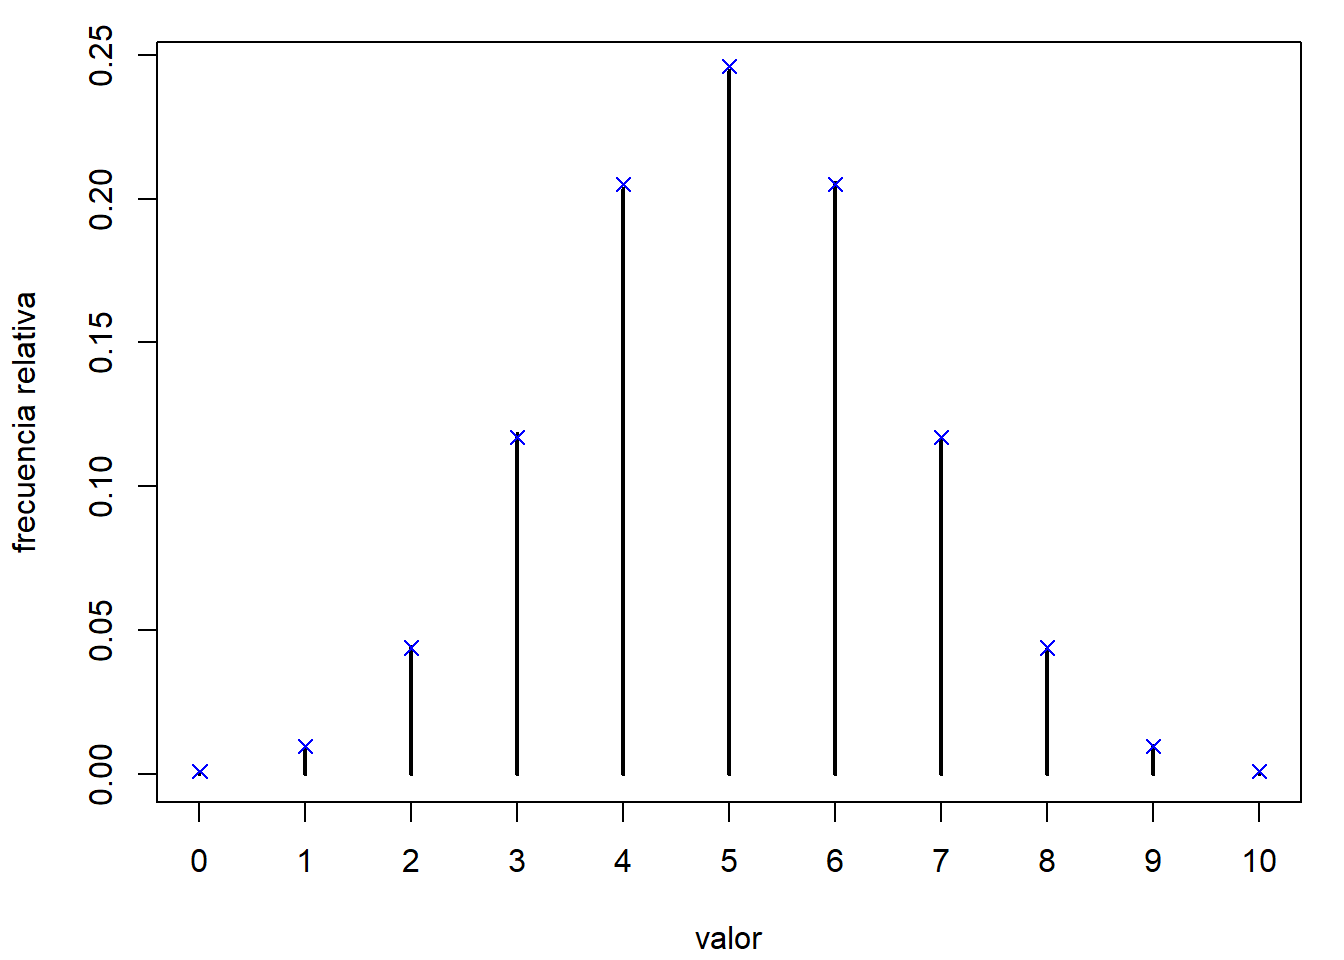
\includegraphics[width=0.7\linewidth]{06-Metodos_generales_discretas_files/figure-latex/comprfmp-1} 

}

\caption{Comparación de las frecuencias relativas de los valores generados con las probabilidades teóricas.}\label{fig:comprfmp}
\end{figure}

\begin{Shaded}
\begin{Highlighting}[]
\NormalTok{res <-}\StringTok{ }\KeywordTok{as.data.frame}\NormalTok{(res)}
\KeywordTok{names}\NormalTok{(res) <-}\StringTok{ }\KeywordTok{c}\NormalTok{(}\StringTok{"x"}\NormalTok{, }\StringTok{"psim"}\NormalTok{)}
\NormalTok{res}\OperatorTok{$}\NormalTok{pteor <-}\StringTok{ }\NormalTok{fmp}
\NormalTok{res}
\end{Highlighting}
\end{Shaded}

\begin{verbatim}
##     x    psim        pteor
## 1   0 0.00107 0.0009765625
## 2   1 0.00990 0.0097656250
## 3   2 0.04432 0.0439453125
## 4   3 0.11778 0.1171875000
## 5   4 0.20425 0.2050781250
## 6   5 0.24375 0.2460937500
## 7   6 0.20454 0.2050781250
## 8   7 0.11898 0.1171875000
## 9   8 0.04419 0.0439453125
## 10  9 0.01023 0.0097656250
## 11 10 0.00099 0.0009765625
\end{verbatim}

\begin{Shaded}
\begin{Highlighting}[]
\CommentTok{# Errores}
\KeywordTok{max}\NormalTok{(}\KeywordTok{abs}\NormalTok{(res}\OperatorTok{$}\NormalTok{psim }\OperatorTok{-}\StringTok{ }\NormalTok{res}\OperatorTok{$}\NormalTok{pteor))}
\end{Highlighting}
\end{Shaded}

\begin{verbatim}
## [1] 0.00234375
\end{verbatim}

\begin{Shaded}
\begin{Highlighting}[]
\KeywordTok{max}\NormalTok{(}\KeywordTok{abs}\NormalTok{(res}\OperatorTok{$}\NormalTok{psim }\OperatorTok{-}\StringTok{ }\NormalTok{res}\OperatorTok{$}\NormalTok{pteor) }\OperatorTok{/}\StringTok{ }\NormalTok{res}\OperatorTok{$}\NormalTok{pteor)}
\end{Highlighting}
\end{Shaded}

\begin{verbatim}
## [1] 0.09568
\end{verbatim}

\begin{remark}
\iffalse{} {Nota: } \fi{}Puede ocurrir que no todos los valores sean generados en la simulación.
En el código anterior si \texttt{length(x)\ \textgreater{}\ length(psim)}, la sentencia
\texttt{res\$pteor\ \textless{}-\ fmp} gererará un error.
Una posible solución sería trabajar con factores (hacer que la función ´rfmp()´ devuelva ´factor(X, levels = x)´). Alternativamente se podría emplear por ejemplo:
\end{remark}

\begin{Shaded}
\begin{Highlighting}[]
\NormalTok{res <-}\StringTok{ }\KeywordTok{data.frame}\NormalTok{(}\DataTypeTok{x =}\NormalTok{ x, }\DataTypeTok{pteor =}\NormalTok{ fmp, }\DataTypeTok{psim =} \DecValTok{0}\NormalTok{)}
\NormalTok{res.sim <-}\StringTok{ }\KeywordTok{table}\NormalTok{(rx)}\OperatorTok{/}\NormalTok{nsim}
\NormalTok{index <-}\StringTok{ }\KeywordTok{match}\NormalTok{(}\KeywordTok{names}\NormalTok{(res.sim), x)}
\NormalTok{res}\OperatorTok{$}\NormalTok{psim[index] <-}\StringTok{ }\NormalTok{res.sim}
\end{Highlighting}
\end{Shaded}

\hypertarget{eficiencia-del-algoritmo-1}{%
\subsection{Eficiencia del algoritmo}\label{eficiencia-del-algoritmo-1}}

Si consideramos la variable aleatoria \(\mathcal{I}\) correspondiente a las etiquetas, su función de masa de probabilidad sería:
\[\begin{array}{l|ccccc}
i & 1 & 2 & \cdots & n & \cdots \\ \hline
P\left( \mathcal{I}=i\right) & p_{1} & p_{2} & \cdots & p_{n} & \cdots 
\end{array}\]
y el número de comparaciones en el paso 3 sería un valor aleatorio de esta variable.
Una medida de la eficiencia del algoritmo de la transformación cuantil es
el número medio de comparaciones:
\[E\left( \mathcal{I}\right) =\sum_i ip_{i}.\]
Realmente, cuando la variable toma un número finito de valores:
\(x_{1}\), \(x_{2}\), \(\ldots\), \(x_{n}\), no sería necesario hacer
la última comprobación \(U>\sum_{i=1}^{n}p_{i}=1\) y se
generaría directamente \(x_{n}\), por lo que el
número medio de comparaciones sería:
\[\sum_{i=1}^{n-1}ip_{i}+\left( n-1\right)  p_{n}.\]

Para disminuir el número esperado de comparaciones podemos
reordenar los valores \(x_{i}\) de forma que las probabilidades
correspondientes sean decrecientes. Esto equivale a considerar
un etiquetado \(l\) de forma que:
\[p_{l\left( 1\right) }\geq p_{l\left( 2\right) }\geq \cdots \geq p_{l\left(
n\right) }\geq \cdots\]

\begin{exercise}[Simulación de una binomial, continuación]
\protect\hypertarget{exr:binom-cuantb}{}{\label{exr:binom-cuantb} \iffalse (Simulación de una binomial, continuación) \fi{} }
\end{exercise}

Repetir el Ejercicio \ref{exr:binom-cuant} anterior ordenando previamente las
probabilidades en orden decreciente y también empleando la
función \texttt{sample} de R.

\begin{Shaded}
\begin{Highlighting}[]
\NormalTok{tini <-}\StringTok{ }\KeywordTok{proc.time}\NormalTok{()}

\NormalTok{ncomp <-}\StringTok{ }\DecValTok{0}
\NormalTok{ind <-}\StringTok{ }\KeywordTok{order}\NormalTok{(fmp, }\DataTypeTok{decreasing=}\OtherTok{TRUE}\NormalTok{)}
\NormalTok{rx <-}\StringTok{ }\KeywordTok{rfmp}\NormalTok{(x[ind], fmp[ind], nsim)}

\NormalTok{tiempo <-}\StringTok{ }\KeywordTok{proc.time}\NormalTok{() }\OperatorTok{-}\StringTok{ }\NormalTok{tini}
\NormalTok{tiempo}
\end{Highlighting}
\end{Shaded}

\begin{verbatim}
##    user  system elapsed 
##    0.12    0.00    0.15
\end{verbatim}

\begin{Shaded}
\begin{Highlighting}[]
\CommentTok{# Número de comparaciones}
\NormalTok{ncomp}\OperatorTok{/}\NormalTok{nsim}
\end{Highlighting}
\end{Shaded}

\begin{verbatim}
## [1] 3.08969
\end{verbatim}

\begin{Shaded}
\begin{Highlighting}[]
\KeywordTok{sum}\NormalTok{((}\DecValTok{1}\OperatorTok{:}\KeywordTok{length}\NormalTok{(x))}\OperatorTok{*}\NormalTok{fmp[ind]) }\CommentTok{# Valor teórico}
\end{Highlighting}
\end{Shaded}

\begin{verbatim}
## [1] 3.083984
\end{verbatim}

Como ya se comentó, en \texttt{R} se recomienda emplear la función \texttt{sample}
(implementa eficientemente el método de Alias descrito en la Sección \ref{alias}):

\begin{Shaded}
\begin{Highlighting}[]
\KeywordTok{system.time}\NormalTok{( rx <-}\StringTok{ }\KeywordTok{sample}\NormalTok{(x, nsim, }\DataTypeTok{replace =} \OtherTok{TRUE}\NormalTok{, }\DataTypeTok{prob =}\NormalTok{ fmp) )}
\end{Highlighting}
\end{Shaded}

\begin{verbatim}
##    user  system elapsed 
##    0.02    0.00    0.02
\end{verbatim}

\hypertarget{muxe9todo-de-la-tabla-guuxeda}{%
\section{Método de la tabla guía}\label{muxe9todo-de-la-tabla-guuxeda}}

La idea consiste en construir \(m\) subintervalos equiespaciados
contenidos en \([0,1]\) de la forma
\[I_{j}=\left[ u_{j},u_{j+1}\right) =\left[ \frac{j-1}{m},\frac{j}{m}\right) 
\text{ para }j=1,2,\ldots ,m\]
y utilizarlos como punto de partida para la búsqueda.
En una tabla guía se almancenan los indices de los cuantiles
correspondientes a los extremos inferiores de los intervalos:
\[g_{j}=Q_{\mathcal{I}}(u_{j})=\inf \left\{ i:F_{i}\geq u_{j}=\frac{j-1}{m}\right\}\]

El punto de partida para un valor \(U\) será \(g_{j_{0}}\) siendo:
\[j_{0}=\left\lfloor mU\right\rfloor +1\]

\begin{center}\includegraphics[width=0.7\linewidth]{images/tablaguia2} \end{center}

En este caso, puede verse que una cota del número medio de comparaciones es:
\[E\left( N\right) \leq 1+\frac{n}{m}\]

\begin{conjecture}[de simulación mediante una tabla guía]
\protect\hypertarget{cnj:unnamed-chunk-18}{}{\label{cnj:unnamed-chunk-18} \iffalse (de simulación mediante una tabla guía) \fi{} }

Inicialización:

\begin{enumerate}
\def\labelenumi{\arabic{enumi}.}
\item
  Hacer \(F_{1}=p_{1}\).
\item
  Desde \(i=2\) hasta \(n\) hacer \(F_{i}=F_{i-1}+p_{i}\).
\end{enumerate}

Cálculo de la tabla guía:

\begin{enumerate}
\def\labelenumi{\arabic{enumi}.}
\item
  Hacer \(g_{1}=1\) e \(i=1\).
\item
  Desde \(j=2\) hasta \(m\) hacer

  2.a Mientras \((j-1)/m>F_{i}\) hacer \(i=i+1\).

  2.b \(g_{j}=i\)
\end{enumerate}

Simulación mediante tabla guía:

\begin{enumerate}
\def\labelenumi{\arabic{enumi}.}
\item
  Generar \(U\sim \mathcal{U}\left( 0,1\right)\).
\item
  Hacer \(j=\left\lfloor mU\right\rfloor +1\).
\item
  Hacer \(i=g_{j}\).
\item
  Mientras \(U>F_{i}\) hacer \(i=i+1\).
\item
  Devolver \(X=x_{i}\).
\end{enumerate}
\end{conjecture}

\begin{exercise}[Simulación de una binomial mediante tabla guía]
\protect\hypertarget{exr:binom-tabla}{}{\label{exr:binom-tabla} \iffalse (Simulación de una binomial mediante tabla guía) \fi{} }
\end{exercise}

Diseñar una rutina que permita generar \(nsim\) valores de una
distribución discreta usando una tabla guía.
Repetir el Ejercicio \ref{exr:binom-cuant} anterior empleando esta rutina con \(m=n-1\).

\begin{Shaded}
\begin{Highlighting}[]
\NormalTok{rfmp.tabla <-}\StringTok{ }\ControlFlowTok{function}\NormalTok{(x, }\DataTypeTok{prob =} \DecValTok{1}\OperatorTok{/}\KeywordTok{length}\NormalTok{(x), m, }\DataTypeTok{nsim =} \DecValTok{1000}\NormalTok{) \{}
  \CommentTok{# Simulación v.a. discreta a partir de función de masa de probabilidad}
  \CommentTok{# por tabla guia de tamaño m}
  \CommentTok{# Inicializar tabla y FD}
\NormalTok{  Fx <-}\StringTok{ }\KeywordTok{cumsum}\NormalTok{(prob)}
\NormalTok{  g <-}\StringTok{ }\KeywordTok{rep}\NormalTok{(}\DecValTok{1}\NormalTok{,m)}
\NormalTok{  i <-}\StringTok{ }\DecValTok{1}
  \ControlFlowTok{for}\NormalTok{(j }\ControlFlowTok{in} \DecValTok{2}\OperatorTok{:}\NormalTok{m) \{}
    \ControlFlowTok{while}\NormalTok{ (Fx[i] }\OperatorTok{<}\StringTok{ }\NormalTok{(j}\DecValTok{-1}\NormalTok{)}\OperatorTok{/}\NormalTok{m) i <-}\StringTok{ }\NormalTok{i}\OperatorTok{+}\DecValTok{1}
\NormalTok{    g[j] <-}\StringTok{ }\NormalTok{i}
\NormalTok{  \}}
  \CommentTok{# Generar valores}
\NormalTok{  X <-}\StringTok{ }\KeywordTok{numeric}\NormalTok{(nsim)}
\NormalTok{  U <-}\StringTok{ }\KeywordTok{runif}\NormalTok{(nsim)}
  \ControlFlowTok{for}\NormalTok{(j }\ControlFlowTok{in} \DecValTok{1}\OperatorTok{:}\NormalTok{nsim) \{}
\NormalTok{    i <-}\StringTok{ }\NormalTok{g[}\KeywordTok{floor}\NormalTok{(U[j]}\OperatorTok{*}\NormalTok{m)}\OperatorTok{+}\DecValTok{1}\NormalTok{]}
    \ControlFlowTok{while}\NormalTok{ (Fx[i] }\OperatorTok{<}\StringTok{ }\NormalTok{U[j]) i <-}\StringTok{ }\NormalTok{i }\OperatorTok{+}\StringTok{ }\DecValTok{1}
\NormalTok{    X[j] <-}\StringTok{ }\NormalTok{x[i]}
\NormalTok{  \}}
  \KeywordTok{return}\NormalTok{(X)}
\NormalTok{\}}

\KeywordTok{system.time}\NormalTok{( rx <-}\StringTok{ }\KeywordTok{rfmp.tabla}\NormalTok{(x, fmp, n}\DecValTok{-1}\NormalTok{, nsim) )}
\end{Highlighting}
\end{Shaded}

\begin{verbatim}
##    user  system elapsed 
##    0.12    0.00    0.14
\end{verbatim}

Análisis de los resultados:

\begin{Shaded}
\begin{Highlighting}[]
\NormalTok{res <-}\StringTok{ }\KeywordTok{table}\NormalTok{(rx)}\OperatorTok{/}\NormalTok{nsim}
\KeywordTok{plot}\NormalTok{(res, }\DataTypeTok{ylab =} \StringTok{"frecuencia relativa"}\NormalTok{, }\DataTypeTok{xlab =} \StringTok{"valores"}\NormalTok{)}
\KeywordTok{points}\NormalTok{(x, fmp, }\DataTypeTok{pch =} \DecValTok{4}\NormalTok{)  }\CommentTok{# Comparación teórica}
\end{Highlighting}
\end{Shaded}

\begin{figure}[!htb]

{\centering 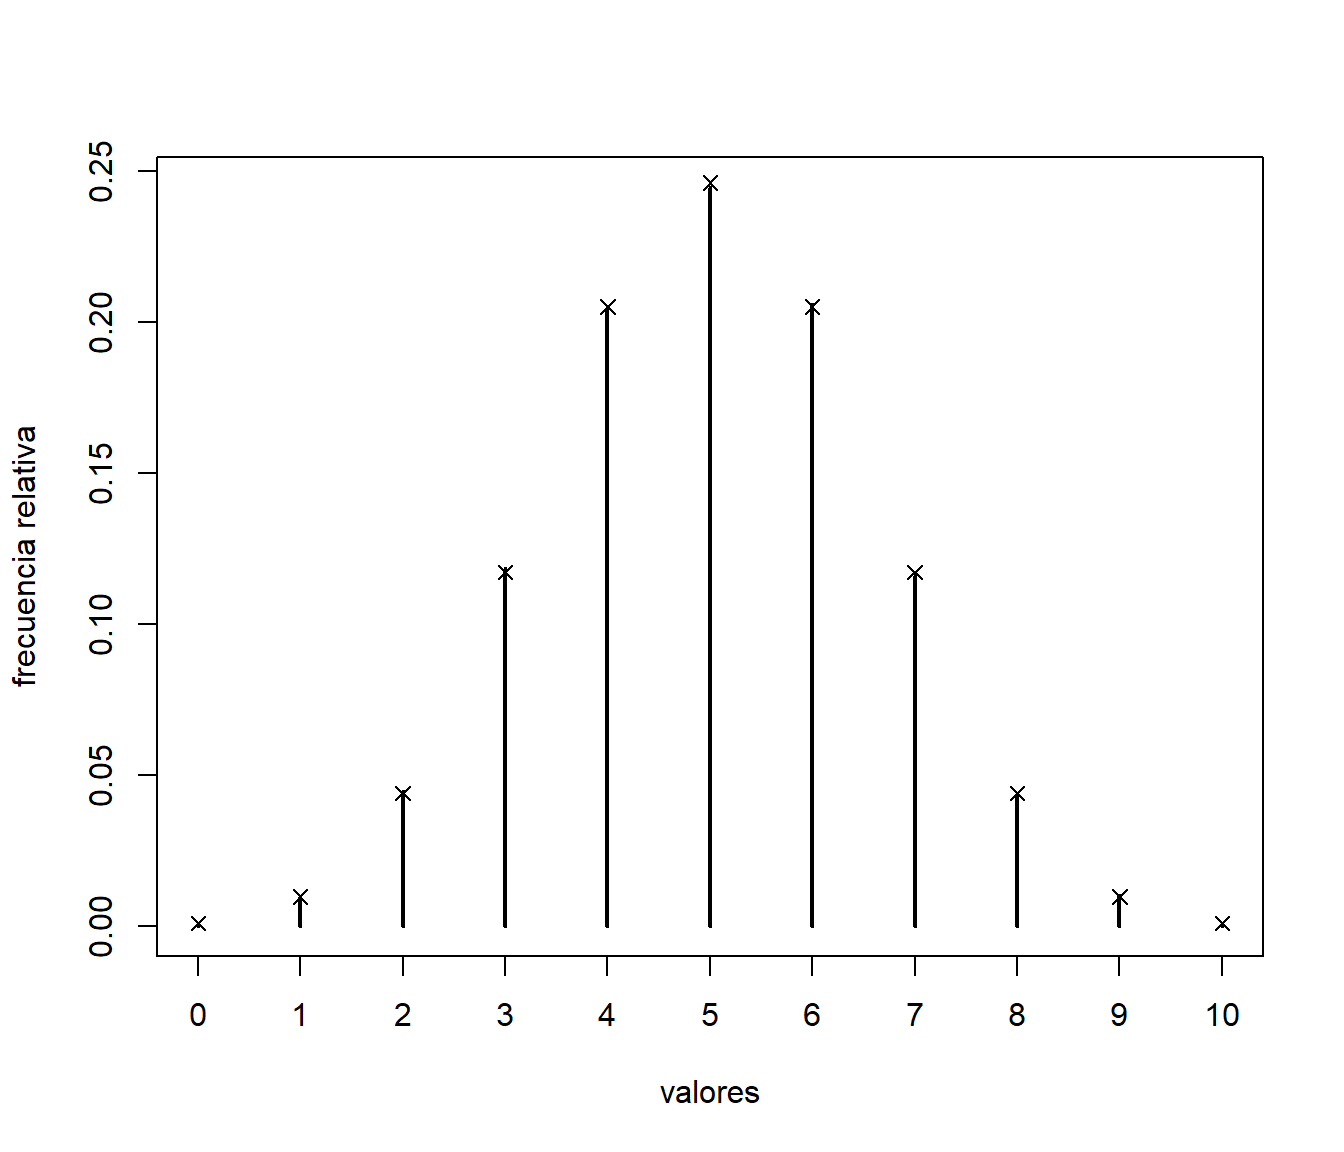
\includegraphics[width=0.7\linewidth]{06-Metodos_generales_discretas_files/figure-latex/comptabla-1} 

}

\caption{Comparación de las frecuencias relativas de los valores generados con las probabilidades teóricas.}\label{fig:comptabla}
\end{figure}

\hypertarget{alias}{%
\section{Método de Alias}\label{alias}}

Se basa en representar la distribución de \(X\) como una mixtura
(uniforme) de variables dicotómicas (Walker, 1977):
\[Q^{(i)}=\left\{ 
\begin{array}{ll}
x_{i} & \text{con prob. } q_{i} \\ 
x_{a_{i}} & \text{con prob. } 1-q_{i}
\end{array}
\ \right.\]

La idea para construir estas variables es ``tomar prestada'' parte de la probabilidad de los valores más probables (ricos) para asignársela a los valores menos probables (pobres), almacenando en \(a_i\) el índice del valor de donde procede.
El algoritmo ``Robin Hood'' de inicialización (Kronmal y Peterson, 1979) es el siguiente:

\begin{enumerate}
\def\labelenumi{\arabic{enumi}.}
\item
  Desde \(i=1\) hasta \(n\) hacer \(q_{i}=np_{i}\).
\item
  Establecer \(L=\left\{ l:q_{l}<1\right\}\) y
  \(H=\left\{ h:q_{h}\geq 1\right\}\).
\item
  Si \(L\) ó \(H\) vacios terminar.
\item
  Seleccionar \(l\in L\) y \(h\in H\).
\item
  Hacer \(a_{l}=h\).
\item
  Eliminar \(l\) de \(L\).
\item
  Hacer \(q_{h}=q_{h}-\left( 1-q_{l}\right)\).
\item
  Si \(q_{h}<1\) mover \(h\) de \(H\) a \(L\).
\item
  Ir al paso 3.
\end{enumerate}

\begin{figure}[!htb]

{\centering \includegraphics[width=0.7\linewidth]{images/alias2} 

}

\caption{Pasos del algoritmo de inicialización del método Alias.}\label{fig:unnamed-chunk-20}
\end{figure}

El algoritmo para generar las simulaciones es el estándar del método de composición:

\begin{enumerate}
\def\labelenumi{\arabic{enumi}.}
\item
  Generar \(U,V\sim \mathcal{U}\left( 0,1\right)\).
\item
  Hacer \(i=\left\lfloor nU\right\rfloor +1\).
\item
  Si \(V<q_{i}\) devolver \(X=x_{i}\).
\item
  En caso contrario devolver \(X=x_{a_{i}}\).
\end{enumerate}

Este algoritmo es muy eficiente y es el implementado en la función \texttt{sample} de R.

\begin{exercise}[Simulación de una binomial mediante en método de Alias]
\protect\hypertarget{exr:binom-alias}{}{\label{exr:binom-alias} \iffalse (Simulación de una binomial mediante en método de Alias) \fi{} }
\end{exercise}

Diseñar una rutina que permita generar \(nsim\) valores de una
distribución discreta usando el método de Alias.
Repetir el Ejercicio \ref{exr:binom-cuant} anterior empleando esta rutina.

\begin{Shaded}
\begin{Highlighting}[]
\NormalTok{rfmp.alias <-}\StringTok{ }\ControlFlowTok{function}\NormalTok{(x, }\DataTypeTok{prob =} \DecValTok{1}\OperatorTok{/}\KeywordTok{length}\NormalTok{(x), }\DataTypeTok{nsim =} \DecValTok{1000}\NormalTok{) \{}
  \CommentTok{# Inicializar tablas}
\NormalTok{  a <-}\StringTok{ }\KeywordTok{numeric}\NormalTok{(}\KeywordTok{length}\NormalTok{(x))}
\NormalTok{  q <-}\StringTok{ }\NormalTok{prob}\OperatorTok{*}\KeywordTok{length}\NormalTok{(x)}
\NormalTok{  low <-}\StringTok{ }\NormalTok{q }\OperatorTok{<}\StringTok{ }\DecValTok{1}
\NormalTok{  high <-}\StringTok{ }\KeywordTok{which}\NormalTok{(}\OperatorTok{!}\NormalTok{low)}
\NormalTok{  low <-}\StringTok{ }\KeywordTok{which}\NormalTok{(low)}
  \ControlFlowTok{while}\NormalTok{ (}\KeywordTok{length}\NormalTok{(high) }\OperatorTok{&&}\StringTok{ }\KeywordTok{length}\NormalTok{(low)) \{}
\NormalTok{    l <-}\StringTok{ }\NormalTok{low[}\DecValTok{1}\NormalTok{]}
\NormalTok{    h <-}\StringTok{ }\NormalTok{high[}\DecValTok{1}\NormalTok{]}
\NormalTok{    a[l] <-}\StringTok{ }\NormalTok{h}
\NormalTok{    q[h] <-}\StringTok{ }\NormalTok{q[h] }\OperatorTok{-}\StringTok{ }\NormalTok{(}\DecValTok{1} \OperatorTok{-}\StringTok{ }\NormalTok{q[l])}
    \ControlFlowTok{if}\NormalTok{ (q[h] }\OperatorTok{<}\StringTok{ }\DecValTok{1}\NormalTok{) \{}
\NormalTok{      high <-}\StringTok{ }\NormalTok{high[}\OperatorTok{-}\DecValTok{1}\NormalTok{]}
\NormalTok{      low[}\DecValTok{1}\NormalTok{] <-}\StringTok{ }\NormalTok{h}
\NormalTok{    \} }\ControlFlowTok{else}\NormalTok{ low <-}\StringTok{ }\NormalTok{low[}\OperatorTok{-}\DecValTok{1}\NormalTok{]}
\NormalTok{  \} }\CommentTok{# while}
  \CommentTok{# Generar valores}
\NormalTok{  V <-}\StringTok{ }\KeywordTok{runif}\NormalTok{(nsim)}
\NormalTok{  i <-}\StringTok{ }\KeywordTok{floor}\NormalTok{(}\KeywordTok{runif}\NormalTok{(nsim)}\OperatorTok{*}\KeywordTok{length}\NormalTok{(x)) }\OperatorTok{+}\StringTok{ }\DecValTok{1}
  \KeywordTok{return}\NormalTok{( x[ }\KeywordTok{ifelse}\NormalTok{( V }\OperatorTok{<}\StringTok{ }\NormalTok{q[i], i, a[i]) ] )}
\NormalTok{\}}


\KeywordTok{system.time}\NormalTok{( rx <-}\StringTok{ }\KeywordTok{rfmp.alias}\NormalTok{(x,fmp,nsim) )}
\end{Highlighting}
\end{Shaded}

\begin{verbatim}
##    user  system elapsed 
##    0.08    0.00    0.09
\end{verbatim}

Análisis de los resultados:

\begin{Shaded}
\begin{Highlighting}[]
\NormalTok{res <-}\StringTok{ }\KeywordTok{table}\NormalTok{(rx)}\OperatorTok{/}\NormalTok{nsim}
\KeywordTok{plot}\NormalTok{(res, }\DataTypeTok{ylab =} \StringTok{"frecuencia relativa"}\NormalTok{, }\DataTypeTok{xlab =} \StringTok{"valores"}\NormalTok{)}
\KeywordTok{points}\NormalTok{(x, fmp, }\DataTypeTok{pch =} \DecValTok{4}\NormalTok{)  }\CommentTok{# Comparación teórica}
\end{Highlighting}
\end{Shaded}

\begin{figure}[!htb]

{\centering 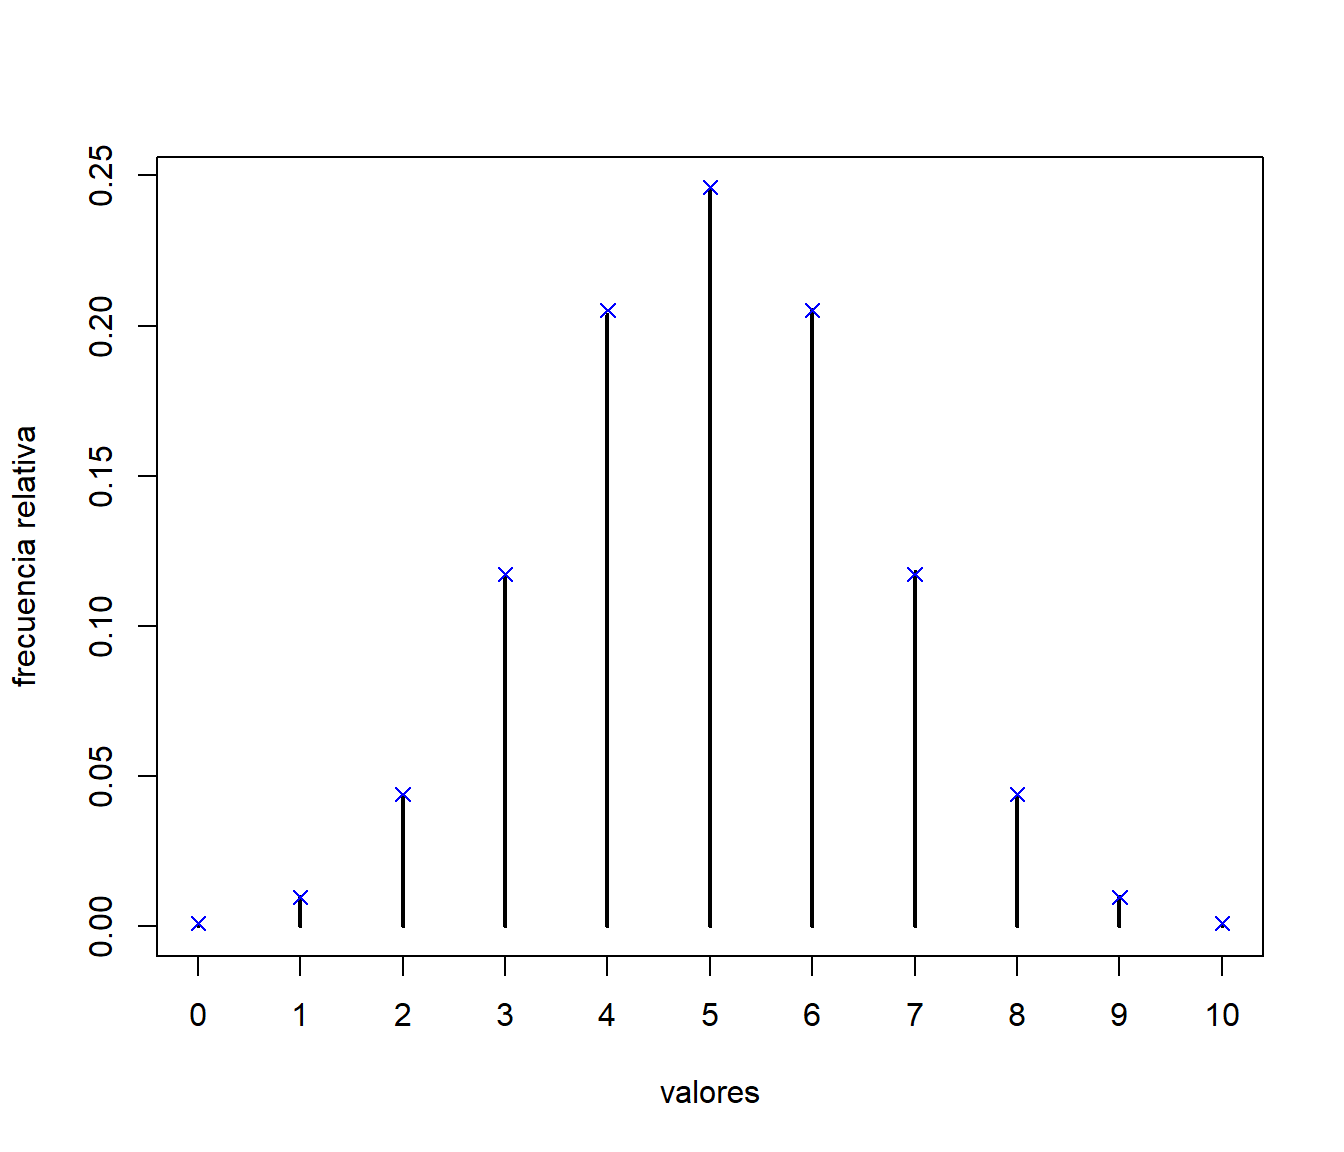
\includegraphics[width=0.7\linewidth]{06-Metodos_generales_discretas_files/figure-latex/compalias-1} 

}

\caption{Comparación de las frecuencias relativas de los valores generados con las probabilidades teóricas.}\label{fig:compalias}
\end{figure}

\hypertarget{simulaciuxf3n-de-una-variable-discreta-con-dominio-infinito}{%
\section{Simulación de una variable discreta con dominio infinito}\label{simulaciuxf3n-de-una-variable-discreta-con-dominio-infinito}}

Los métodos anteriores están pensados para variables que toman
un número finito de valores.
Si la variable discreta tiene dominio infinito no se podrían
almacenar las probabilidades acumuladas, aunque en algunos casos podrían
calcularse de forma recursiva.

\begin{example}[distribución de Poisson]
\protect\hypertarget{exm:unnamed-chunk-22}{}{\label{exm:unnamed-chunk-22} \iffalse (distribución de Poisson) \fi{} }
\end{example}
Una variable \(X\) con distribución de Poisson de parámetro \(\lambda\),
toma los valores \(x_{1}=0\), \(x_{2}=1\), \(\ldots\) con probabilidades:
\[p_{j}=P\left( X=x_{j}\right)  =P\left( X=j-1\right)  =\frac{e^{-\lambda
}\lambda^{j-1}}{\left( j-1\right)  !}\text{, }j=1,2,\ldots\]
En este caso, como:
\[P\left( X=j\right)  =\frac{e^{-\lambda}\lambda^{j}}{j!}
=\frac{\lambda}{j}\frac{e^{-\lambda}\lambda^{j-1}}{\left( j-1\right)  !}
=\frac{\lambda}{j}P\left( X=j-1\right),\]
el algoritmo de inversión con búsqueda secuencial sería:

\begin{enumerate}
\def\labelenumi{\arabic{enumi}.}
\item
  Generar \(U\sim \mathcal{U}\left( 0,1\right)\).
\item
  Hacer \(I=0\), \(p=e^{-\lambda}\) y \(S=p\).
\item
  Mientras \(U>S\) hacer \(I=I+1\), \(p=\frac{\lambda}{I}p\) y \(S=S+p\).
\item
  Devolver \(X=I\).
\end{enumerate}

Hay modificaciones de los algoritmos anteriores, e.g.~incluyendo
una búsqueda secuencial en la cola de la distribución, para
estos casos.

Como alternativa, siempre se puede pensar en truncar la distribución,
eliminando los valores muy poco probables (teniendo en
cuenta el número de generaciones que se pretenden realizar),
de esta forma la distribución de las simulaciones sería aproximada.

\hypertarget{cuxe1lculo-directo-de-la-funciuxf3n-cuantil}{%
\section{Cálculo directo de la función cuantil}\label{cuxe1lculo-directo-de-la-funciuxf3n-cuantil}}

En ocasiones el método de la transformación cuantil puede acelerarse
computacionalmente porque, mediante cálculos directos, es posible
encontrar el valor de la función cuantil en cualquier \(U\),
evitando el bucle de búsqueda.
Normalmente se realiza mediante truncamiento de una distribución continua.

\begin{example}[distribución uniforme discreta]
\protect\hypertarget{exm:unnamed-chunk-23}{}{\label{exm:unnamed-chunk-23} \iffalse (distribución uniforme discreta) \fi{} }
\end{example}

La función de masa de probabilidad de una distribución uniforme discreta
en \(\{1,2,\ldots,n\}\) viene dada por
\[p_{j}=\frac{1}{n}\text{, para }j=1,2,\ldots n.\]

Pueden generarse valores de esta distribución de forma muy eficiente
truncando la distribución uniforme:

\begin{enumerate}
\def\labelenumi{\arabic{enumi}.}
\item
  Generar \(U\sim \mathcal{U}\left( 0,1\right)\).
\item
  Devolver \(X=\left\lfloor nU\right\rfloor + 1\).
\end{enumerate}

\begin{example}[distribución geométrica]
\protect\hypertarget{exm:unnamed-chunk-24}{}{\label{exm:unnamed-chunk-24} \iffalse (distribución geométrica) \fi{} }
\end{example}

La función de masa de probabilidad de una distribución geométrica es:
\[P\left( X=j\right)  =P\left( I=j+1\right)  =p\left( 1-p\right)^{j}\text{,
}j=0,1,\ldots\]

Si se considera como variable aleatoria continua auxiliar una
exponencial, con función de distribución
\(G\left( x\right) = 1-e^{-\lambda x}\) si \(x\geq0\),
se tiene que:
\[\begin{aligned}
G\left( i\right) - G\left( i-1\right)   
& = 1-e^{-\lambda i}-\left(1-e^{-\lambda\left( i-1\right) }\right)  
= e^{-\lambda\left( i-1\right)}-e^{-\lambda i}\\
& = e^{-\lambda\left( i-1\right)  }\left( 1-e^{-\lambda}\right)  
= \left( 1-e^{-\lambda}\right)  \left( e^{-\lambda}\right)^{i-1} \\
& = p\left(1-p\right)^{i-1},
\end{aligned}\]
tomando \(p=1-e^{-\lambda}\).
De donde se obtendría el algoritmo:

\begin{enumerate}
\def\labelenumi{\arabic{enumi}.}
\setcounter{enumi}{-1}
\item
  Hacer \(\lambda=-\ln\left( 1-p\right)\).
\item
  Generar \(U\sim \mathcal{U}\left( 0,1\right)\).
\item
  Hacer \(T=-\frac{\ln U}{\lambda}\).
\item
  Devolver \(X=\left\lfloor T\right\rfloor\).
\end{enumerate}

\hypertarget{otros-muxe9todos}{%
\section{Otros métodos}\label{otros-muxe9todos}}

\begin{itemize}
\item
  Aceptación-Rechazo: Este método también sería directamente aplicable al
  caso discreto. En principio habría que considerar una variable
  auxiliar discreta con el mismo soporte, pero también hay modificaciones
  para variables auxiliares continuas.
\item
  Método de composición: este es otro método directamente aplicable y
  que se emplea en el método de Alias (descrito en la Sección \ref{alias})
\item
  Hay otros métodos que tratan de reducir el número medio de comparaciones
  de la búsqueda secuencial, por ejemplo los árboles (binarios) de Huffman
  (e.g.~Cao, 2002, Sección 4.2).
\end{itemize}

\begin{exercise}[Simulación de una distribución mixta mediante el método de inversión generalizado]
\protect\hypertarget{exr:mixta-cuantil}{}{\label{exr:mixta-cuantil} \iffalse (Simulación de una distribución mixta mediante el método de inversión generalizado) \fi{} }
\end{exercise}

Considera la variable aleatoria con función
de distribución dada por:
\[F(x)=\left\{
\begin{array}
[c]{cl}0 & \mbox{si $x<0$}\\
\frac{x}{2}+\frac{1}{10} & \mbox{si $x\in[0,\frac{1}{5})$}\\
x+\frac{1}{10} & \mbox{si $x\in[\frac{1}{5},\frac{9}{10}]$}\\
1 & \mbox{en otro caso}
\end{array}
\right.\]

Función de distribución:

\begin{Shaded}
\begin{Highlighting}[]
\NormalTok{fdistr <-}\StringTok{ }\ControlFlowTok{function}\NormalTok{(x) \{}
\KeywordTok{ifelse}\NormalTok{(x }\OperatorTok{<}\StringTok{ }\DecValTok{0}\NormalTok{, }\DecValTok{0}\NormalTok{,}
    \KeywordTok{ifelse}\NormalTok{(x }\OperatorTok{<}\StringTok{ }\DecValTok{1}\OperatorTok{/}\DecValTok{5}\NormalTok{, x}\OperatorTok{/}\DecValTok{2} \OperatorTok{+}\StringTok{ }\DecValTok{1}\OperatorTok{/}\DecValTok{10}\NormalTok{,}
        \KeywordTok{ifelse}\NormalTok{(x }\OperatorTok{<=}\StringTok{ }\DecValTok{9}\OperatorTok{/}\DecValTok{10}\NormalTok{, x }\OperatorTok{+}\StringTok{ }\DecValTok{1}\OperatorTok{/}\DecValTok{10}\NormalTok{, }\DecValTok{1}\NormalTok{) ) )}
\NormalTok{\}}
\CommentTok{# Empleando ifelse se complica un poco más pero el resultado es una función vectorial.}
\KeywordTok{curve}\NormalTok{(}\KeywordTok{fdistr}\NormalTok{(x), }\DataTypeTok{from =} \FloatTok{-0.1}\NormalTok{, }\DataTypeTok{to =} \FloatTok{1.1}\NormalTok{, }\DataTypeTok{type =} \StringTok{'s'}\NormalTok{, }
      \DataTypeTok{main =} \StringTok{'Función de distribución')}
\StringTok{# Discontinuidades en 0 y 1/5}
\StringTok{abline(h = c(1/10, 2/10, 3/10), lty = 2) }
\end{Highlighting}
\end{Shaded}

\begin{center}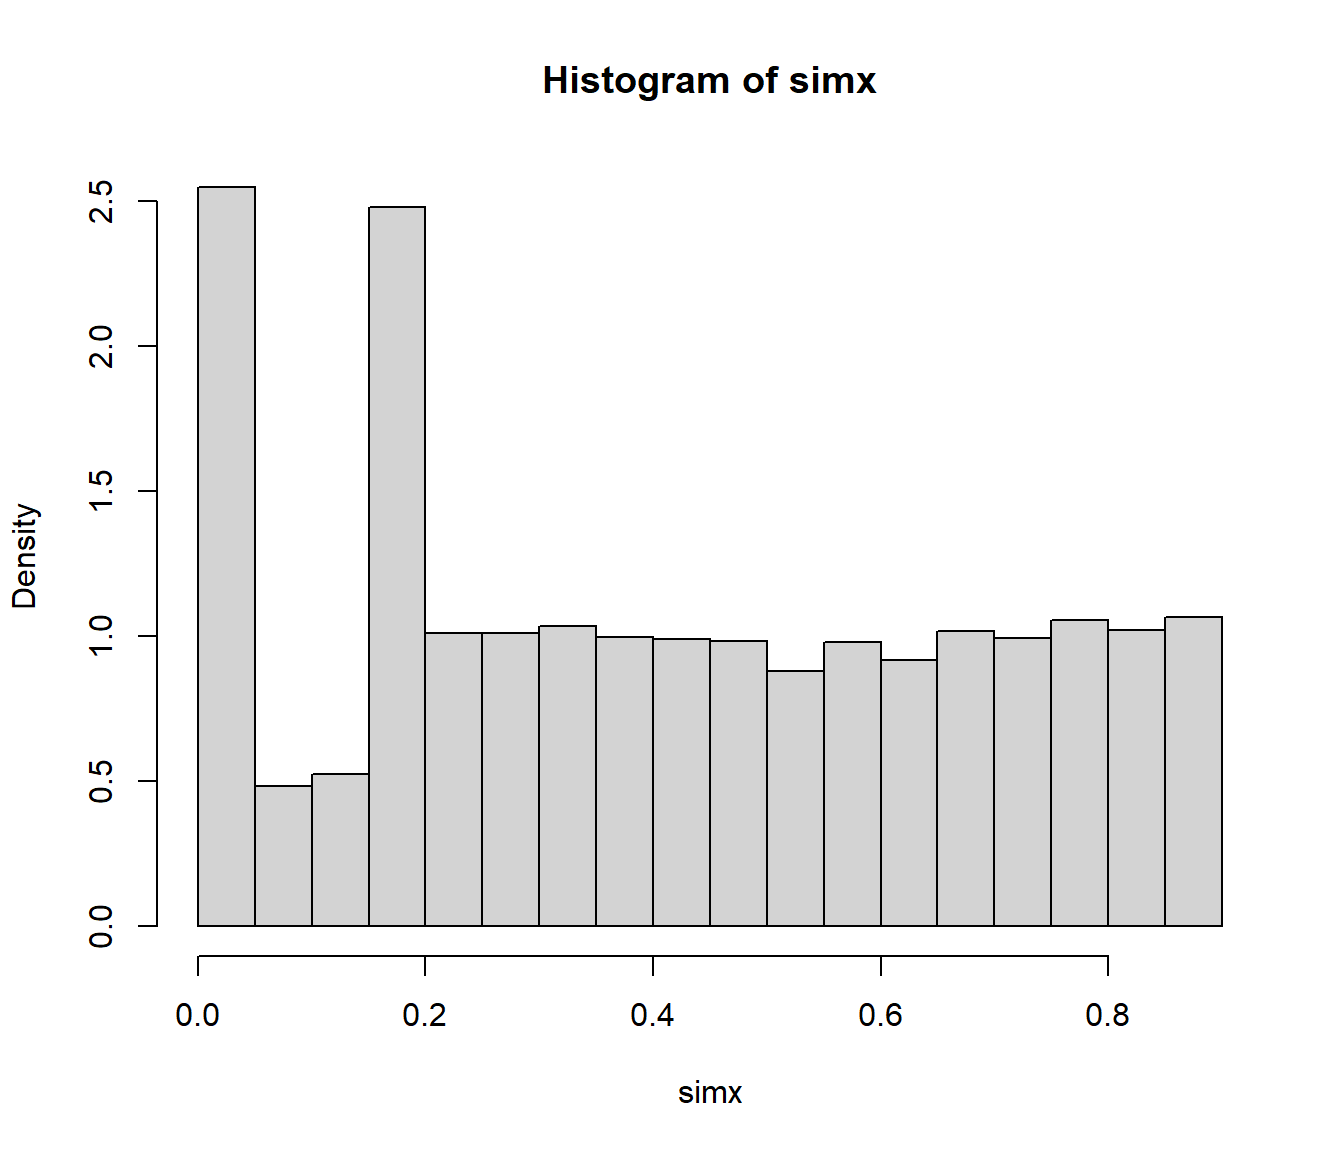
\includegraphics[width=0.7\linewidth]{06-Metodos_generales_discretas_files/figure-latex/unnamed-chunk-25-1} \end{center}

\textbf{Nota}: Esta variable toma los valores 0 y 1/5 con probabilidad 1/10.

\begin{enumerate}
\def\labelenumi{\alph{enumi})}
\item
  Diseña un algoritmo basándote en el método de inversión generalizado
  para generar observaciones de esta variable.

  El algoritmo general es siempre el mismo. Empleando la función cuantil:
  \[Q\left( u\right) = \inf \left\{ x\in \mathbb{R}:F\left( x\right) 
  \geq u\right\},\]
  el algoritmo sería:

  \begin{enumerate}
  \def\labelenumii{\arabic{enumii}.}
  \item
    Generar \(U\sim \mathcal{U}\left( 0,1\right)\)
  \item
    Devolver \(X=Q\left( U\right)\)
  \end{enumerate}

  En este caso concreto:

  \begin{enumerate}
  \def\labelenumii{\arabic{enumii}.}
  \item
    Generar \(U\sim \mathcal{U}\left( 0,1\right)\)
  \item
    Si \(U < \frac{1}{10}\) devolver \(X = 0\)
  \item
    Si \(U < \frac{2}{10}\) devolver \(X = 2(U - \frac{1}{10})\)
  \item
    Si \(U < \frac{3}{10}\) devolver \(X = \frac{2}{10}\)
  \item
    En caso contrario devolver \(X = U - \frac{1}{10}\)
  \end{enumerate}
\item
  Implementa el algoritmo en una función que permita generar \(nsim\)
  valores de la variable.

\begin{Shaded}
\begin{Highlighting}[]
\CommentTok{# Función cuantil:}
\NormalTok{fquant <-}\StringTok{ }\ControlFlowTok{function}\NormalTok{(u) }
  \KeywordTok{ifelse}\NormalTok{(u }\OperatorTok{<}\StringTok{ }\DecValTok{1}\OperatorTok{/}\DecValTok{10}\NormalTok{, }\DecValTok{0}\NormalTok{,}
         \KeywordTok{ifelse}\NormalTok{(u }\OperatorTok{<}\StringTok{ }\DecValTok{2}\OperatorTok{/}\DecValTok{10}\NormalTok{, }\DecValTok{2}\OperatorTok{*}\NormalTok{(u }\OperatorTok{-}\StringTok{ }\DecValTok{1}\OperatorTok{/}\DecValTok{10}\NormalTok{),}
                \KeywordTok{ifelse}\NormalTok{(u }\OperatorTok{<}\StringTok{ }\DecValTok{3}\OperatorTok{/}\DecValTok{10}\NormalTok{, }\DecValTok{1}\OperatorTok{/}\DecValTok{5}\NormalTok{, u }\OperatorTok{-}\StringTok{ }\DecValTok{1}\OperatorTok{/}\DecValTok{10}\NormalTok{) ) )}
\CommentTok{# Función para generar nsim valores:}
\NormalTok{rx <-}\StringTok{ }\ControlFlowTok{function}\NormalTok{(nsim) }\KeywordTok{fquant}\NormalTok{(}\KeywordTok{runif}\NormalTok{(nsim))}
\end{Highlighting}
\end{Shaded}

  Ejemplo:

\begin{Shaded}
\begin{Highlighting}[]
\KeywordTok{set.seed}\NormalTok{(}\DecValTok{1}\NormalTok{)}
\NormalTok{nsim <-}\StringTok{ }\DecValTok{10}\OperatorTok{^}\DecValTok{4}
\KeywordTok{system.time}\NormalTok{(simx <-}\StringTok{ }\KeywordTok{rx}\NormalTok{(nsim))}
\end{Highlighting}
\end{Shaded}

\begin{verbatim}
##    user  system elapsed 
##       0       0       0
\end{verbatim}

\begin{Shaded}
\begin{Highlighting}[]
\KeywordTok{hist}\NormalTok{(simx, }\DataTypeTok{breaks =} \StringTok{"FD"}\NormalTok{, }\DataTypeTok{freq =} \OtherTok{FALSE}\NormalTok{)}
\end{Highlighting}
\end{Shaded}

  \begin{center}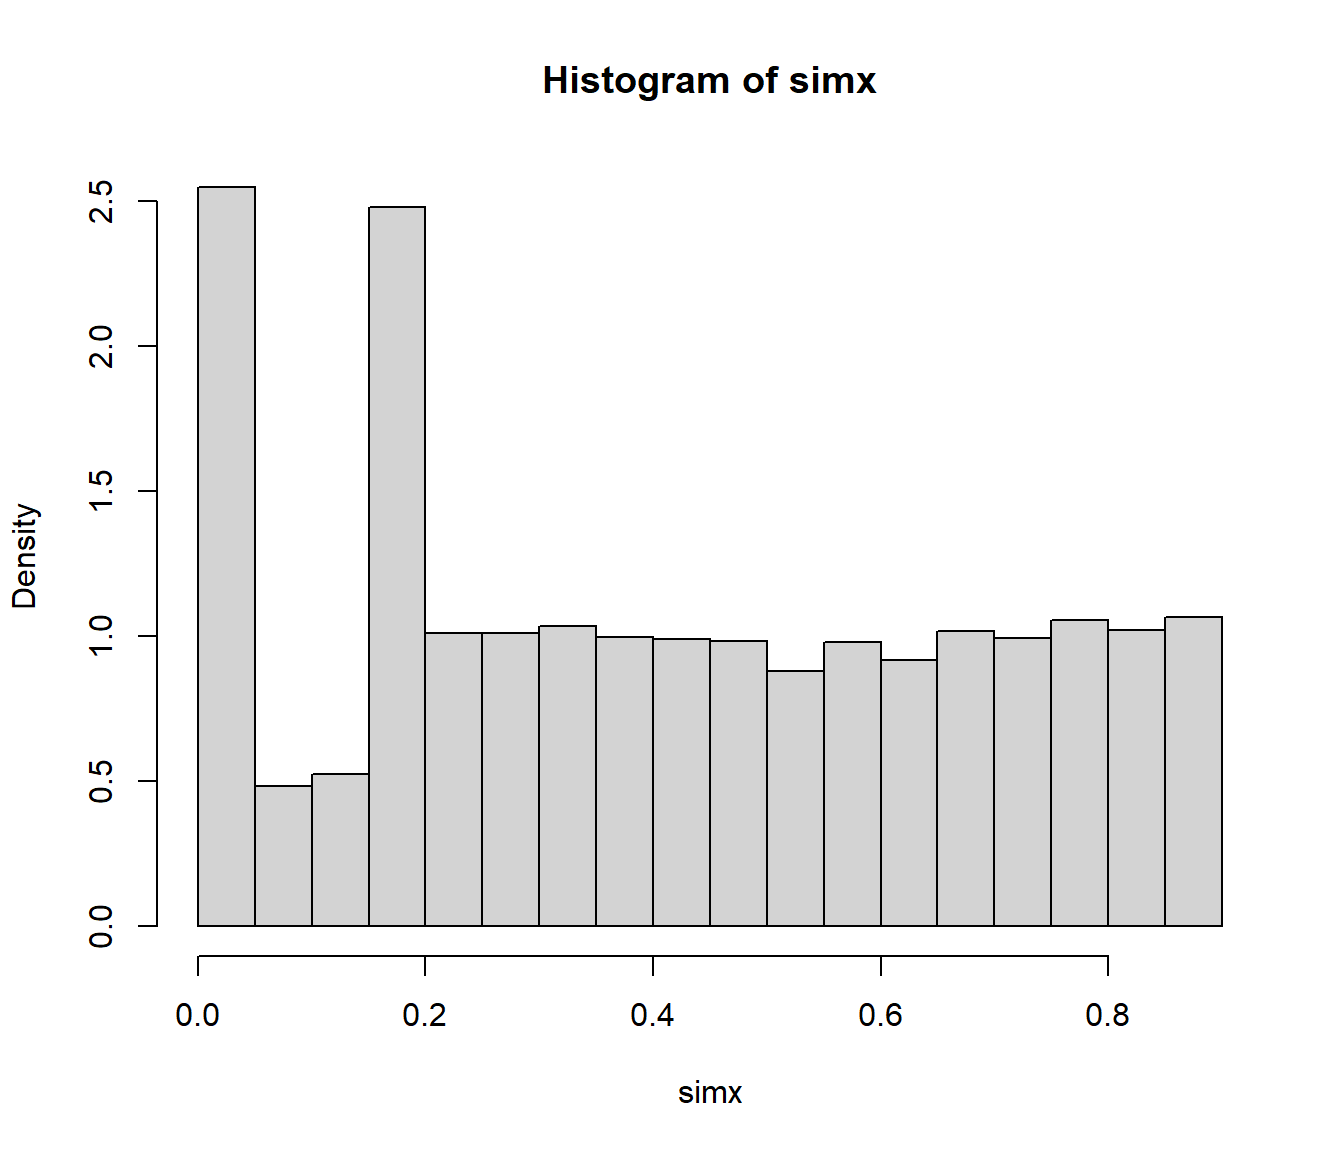
\includegraphics[width=0.7\linewidth]{06-Metodos_generales_discretas_files/figure-latex/unnamed-chunk-27-1} \end{center}

  En este caso como no es una variable absolutamente continua mejor emplear
  la función de distribución para compararla con la teórica:

\begin{Shaded}
\begin{Highlighting}[]
\KeywordTok{curve}\NormalTok{(}\KeywordTok{ecdf}\NormalTok{(simx)(x), }\DataTypeTok{from=} \FloatTok{-0.1}\NormalTok{, }\DataTypeTok{to =} \FloatTok{1.1}\NormalTok{, }\DataTypeTok{type =} \StringTok{"s"}\NormalTok{)}
\KeywordTok{curve}\NormalTok{(}\KeywordTok{fdistr}\NormalTok{(x), }\DataTypeTok{type =} \StringTok{"s"}\NormalTok{, }\DataTypeTok{lty =} \DecValTok{2}\NormalTok{, }\DataTypeTok{add =} \OtherTok{TRUE}\NormalTok{)}
\end{Highlighting}
\end{Shaded}

  \begin{center}\includegraphics[width=0.7\linewidth]{06-Metodos_generales_discretas_files/figure-latex/unnamed-chunk-28-1} \end{center}
\end{enumerate}

\begin{exercise}[propuesto]
\protect\hypertarget{exr:hipergeom}{}{\label{exr:hipergeom} \iffalse (propuesto) \fi{} }
\end{exercise}

Se pretende simular \(nsim=10^{4}\) observaciones de una variable
hipergeométrica (\texttt{dhyper(x,\ m,\ n,\ k)}) de parámetros \(m=\) el número
de grupo multiplicado por 10, \(n=100-m\) y \(k=20\).

\begin{enumerate}
\def\labelenumi{\alph{enumi})}
\item
  Comprobar que el rango de posibles valores de esta variable es
  \texttt{max(0,\ k-n):min(m,\ k)}. Generar los valores empleando el método
  de la transformación cuantil usando búsqueda secuencial. Obtener
  el tiempo de CPU empleado. Aproximar por simulación la función
  de masa de probabilidad, representarla gráficamente y compararla
  con la teórica. Calcular también la media muestral (compararla
  con la teórica \(km/(m+n)\)) y el número medio de comparaciones
  para generar cada observación.
\item
  Repetir el apartado anterior ordenando previamente las
  probabilidades en orden decreciente y también: empleando la
  función \texttt{sample} de R, mediante una tabla guía (con
  \(k-1\) subintervalos) y usando el método de Alias.
\end{enumerate}

\hypertarget{notables-disc}{%
\section{Métodos específicos para generación de distribuciones notables}\label{notables-disc}}

Los comentarios al principio de la Sección \ref{notables-cont} para el caso de variables continuas serían válidos también para distribuciones notables discretas.

Entre los distintos métodos disponibles para la generación de las distribuciones discretas más conocidas podríamos destacar el de la distribución binomial negativa mediante el método de composición (Sección \ref{composicion}).

La distribución binomial negativa, \(BN(r, p)\), puede interpretarse como el número de fracasos antes del \(r\)-ésimo éxito\footnote{La distribución binomial negativa es una generalización de la geométrica y, debido a su reproductividad en el parámetro \(r\), podría simularse como suma de \(r\) variables geométricas. Sin embargo, este algoritmo puede ser muy costoso en tiempo de computación si \(r\) es elevado.} y su función de masa de probabilidad es
\[P(X = i) = \binom{i+r-1}i p^r (1-p)^i \text{, para }i=0,1,\ldots\]

A partir de la propiedad
\[X|_{Y} \sim \text{Pois}\left(  Y\right)  \text{, }Y \sim \operatorname{Gamma} \left( r, \frac{p}{1-p}\right)  \Rightarrow X \sim BN(r, p)\]
se puede deducir el siguiente método específico de simulación.

\textbf{Algoritmo condicional para simular la binomial negativa}

\begin{enumerate}
\def\labelenumi{\arabic{enumi}.}
\item
  Simular \(L \sim \operatorname{Gamma}\left( r, \frac{p}{1-p} \right)\).
\item
  Simular \(X \sim Pois \left( L\right)\).
\item
  Devolver \(X\).
\end{enumerate}

Por este motivo se denominada también a esta distribución \emph{Gamma--Poisson}. Empleando una aproximación similar podríamos generar otras distribuciones, como la \emph{Beta-Binomial}, empleadas habitualmente en Inferencia Bayesiana.

\hypertarget{simulaciuxf3n-de-distribuciones-multivariantes}{%
\chapter{Simulación de distribuciones multivariantes}\label{simulaciuxf3n-de-distribuciones-multivariantes}}

La simulación de vectores aleatorios \(\mathbf{X} =\left( X_1,X_2,\ldots,X_d\right)\) que sigan cierta distribución dada no es tarea siempre sencilla.
En general, no resulta una extensión inmediata del caso unidimensional,
aunque muchos de los algoritmos descritos en los temas anteriores (como el de aceptación-rechazo o el de composición) son válidos para distribuciones multivariantes.
En este caso sin embargo, puede ser mucho más difícil cumplir los requerimientos (e.g.~encontrar una densidad auxiliar adecuada) y los algoritmos obtenidos pueden ser computacionalmente poco eficientes (especialmente si el número de dimensiones es grande).

En las primeras secciones de este capítulo supondremos que se pretende simular una variable aleatoria multidimensional continua \(\mathbf{X}\) con función de densidad conjunta \(f\left( x_1, x_2, \ldots , x_d\right)\) (aunque muchos resultados serán válidos para variables discretas multidimensionales, simplemente cambiando funciones de densidad por las correspondientes de masa de probabilidad).
En la Sección \ref{mult-discr} se tratará brevemente la simulación de vectores aleatorios discretos y de tablas de contingencia, centrándose en el caso bidimensional.

\hypertarget{simulaciuxf3n-de-componentes-independientes}{%
\section{Simulación de componentes independientes}\label{simulaciuxf3n-de-componentes-independientes}}

Si las componentes son independientes y \(f_i\) son las correspondientes densidades marginales, bastará con generar \(X_i \sim f_i\).
Las dificultades aparecerán cuando se quiera simular componentes con una determinada estructura de dependencia.

\begin{example}[simulación de normales independientes]
\protect\hypertarget{exm:normind}{}{\label{exm:normind} \iffalse (simulación de normales independientes) \fi{} }
\end{example}

Si \(\boldsymbol\mu =\left( \mu_1,\mu_2,\ldots,\mu_d\right)^t\) es un vector (de medias) y
\(\Sigma\) es una matriz \(d \times d\) definida positiva (de varianzas-covarianzas), el vector aleatorio \(\mathbf{X}\) sigue una distribución normal multivariante con esos parámetros,
\(\mathbf{X} \sim \mathcal{N}_d\left( \boldsymbol\mu,\Sigma \right)\),
si su función de densidad es de la forma:
\[f(\mathbf x) = \frac{1}{(2\pi)^{n/2}|\Sigma|^{1/2}}
\exp \left( -\frac{1}{2} ( \mathbf x - \boldsymbol \mu)^t \Sigma^{-1} (\mathbf x - \boldsymbol \mu)
\right),\]
donde \(| \Sigma |\) es el determinante de \(\Sigma\).

Si la matriz de covarianzas es diagonal \(\Sigma=diag\left( \sigma_1^2,\sigma_2^2,\ldots,\sigma_d^2\right)\),
entonces las componentes \(X_i \sim \mathcal{N}\left( \mu_i,\sigma_i^2\right)\)
son independientes y podemos simular el vector aleatorio de forma trivial, por ejemplo mediante el siguiente algoritmo:

\begin{conjecture}[de simulación de normales independientes]
\protect\hypertarget{cnj:mnorm-indep}{}{\label{cnj:mnorm-indep} \iffalse (de simulación de normales independientes) \fi{} }

\begin{enumerate}
\def\labelenumi{\arabic{enumi}.}
\item
  Simular \(Z_1, Z_2, \ldots, Z_d \sim \mathcal{N} \left( 0, 1 \right)\) independientes.
\item
  Para \(i = 1, 2, \ldots, d\) hacer \(X_i = \mu_i + \sigma_i Z_i\).
\end{enumerate}
\end{conjecture}

Las funciones implementadas en el paquete base de \texttt{R} permiten simular fácilmente en el caso independiente ya que admiten vectores como parámetros.
Por ejemplo en el caso bidimensional con \(X_1 \sim \mathcal{N}\left( 0, 1\right)\) y \(X_2 \sim \mathcal{N}\left( -1, 0.5^2 \right)\):



\begin{Shaded}
\begin{Highlighting}[]
\NormalTok{f1 <-}\StringTok{ }\ControlFlowTok{function}\NormalTok{(x) }\KeywordTok{dnorm}\NormalTok{(x)}
\NormalTok{f2 <-}\StringTok{ }\ControlFlowTok{function}\NormalTok{(x) }\KeywordTok{dnorm}\NormalTok{(x, }\DecValTok{-1}\NormalTok{, }\FloatTok{0.5}\NormalTok{)}
\KeywordTok{curve}\NormalTok{(f1, }\DecValTok{-3}\NormalTok{, }\DecValTok{3}\NormalTok{, }\DataTypeTok{ylim =} \KeywordTok{c}\NormalTok{(}\DecValTok{0}\NormalTok{, }\KeywordTok{f2}\NormalTok{(}\OperatorTok{-}\DecValTok{1}\NormalTok{)), }\DataTypeTok{ylab =} \StringTok{"fdp"}\NormalTok{)}
\KeywordTok{curve}\NormalTok{(f2, }\DataTypeTok{add =} \OtherTok{TRUE}\NormalTok{, }\DataTypeTok{lty =} \DecValTok{2}\NormalTok{)}
\end{Highlighting}
\end{Shaded}

\begin{figure}[!htb]

{\centering 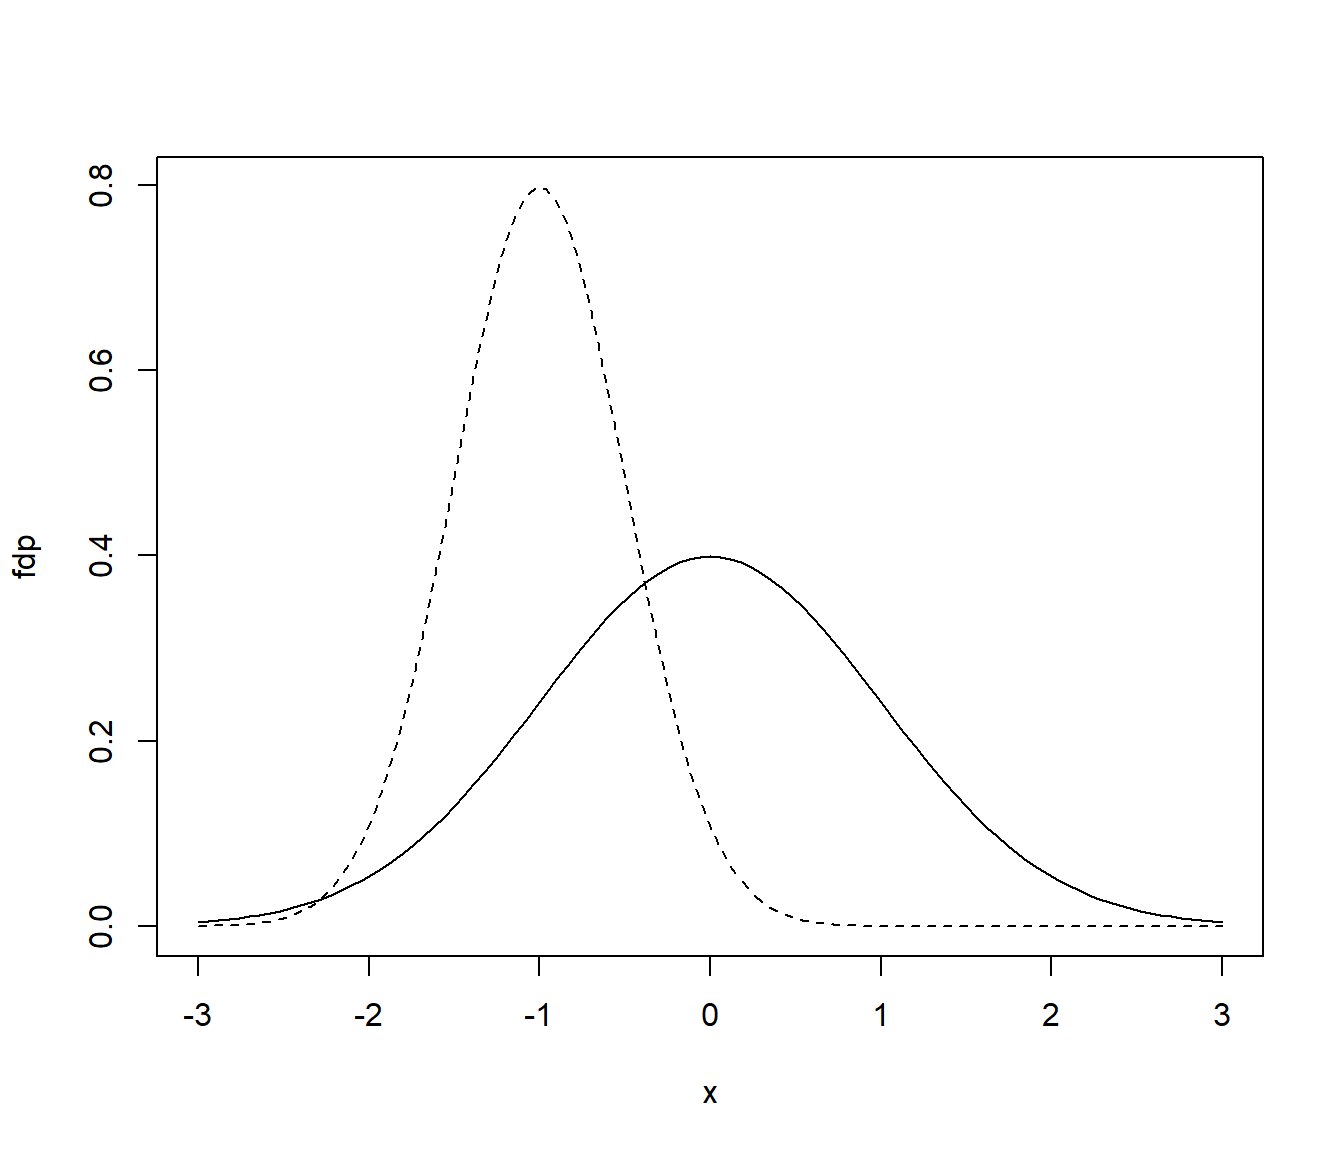
\includegraphics[width=0.7\linewidth]{07-Simulacion_multidimensional_files/figure-latex/normind-plot-1} 

}

\caption{Densidades marginales de las componentes del Ejemplo \ref{exm:normind}.}\label{fig:normind-plot}
\end{figure}

Para simular una generación bastaría con:

\begin{Shaded}
\begin{Highlighting}[]
\KeywordTok{set.seed}\NormalTok{(}\DecValTok{1}\NormalTok{)}
\KeywordTok{rnorm}\NormalTok{(}\DecValTok{2}\NormalTok{, }\KeywordTok{c}\NormalTok{(}\DecValTok{0}\NormalTok{, }\DecValTok{-1}\NormalTok{), }\KeywordTok{c}\NormalTok{(}\DecValTok{1}\NormalTok{, }\FloatTok{0.5}\NormalTok{))}
\end{Highlighting}
\end{Shaded}

\begin{verbatim}
## [1] -0.6264538 -0.9081783
\end{verbatim}

y para simular \texttt{nsim}:

\begin{Shaded}
\begin{Highlighting}[]
\KeywordTok{set.seed}\NormalTok{(}\DecValTok{1}\NormalTok{)}
\NormalTok{nsim <-}\StringTok{ }\DecValTok{5}
\NormalTok{rx <-}\StringTok{ }\KeywordTok{matrix}\NormalTok{(}\KeywordTok{rnorm}\NormalTok{(}\DecValTok{2}\OperatorTok{*}\NormalTok{nsim, }\KeywordTok{c}\NormalTok{(}\DecValTok{0}\NormalTok{, }\DecValTok{-1}\NormalTok{), }\KeywordTok{c}\NormalTok{(}\DecValTok{1}\NormalTok{, }\FloatTok{0.5}\NormalTok{)), }\DataTypeTok{nrow =}\NormalTok{ nsim, }\DataTypeTok{byrow =} \OtherTok{TRUE}\NormalTok{)}
\KeywordTok{colnames}\NormalTok{(rx) <-}\StringTok{ }\KeywordTok{paste0}\NormalTok{(}\StringTok{"X"}\NormalTok{, }\DecValTok{1}\OperatorTok{:}\KeywordTok{ncol}\NormalTok{(rx))}
\NormalTok{rx}
\end{Highlighting}
\end{Shaded}

\begin{verbatim}
##              X1         X2
## [1,] -0.6264538 -0.9081783
## [2,] -0.8356286 -0.2023596
## [3,]  0.3295078 -1.4102342
## [4,]  0.4874291 -0.6308376
## [5,]  0.5757814 -1.1526942
\end{verbatim}

\hypertarget{el-muxe9todo-de-aceptaciuxf3nrechazo}{%
\section{El método de aceptación/rechazo}\label{el-muxe9todo-de-aceptaciuxf3nrechazo}}

El algoritmo de aceptación-rechazo es el mismo que el del caso univariante descrito en la Sección \ref{AR}, la única diferencia es que las densidades son multidimensionales.
Supongamos que la densidad objetivo \(f\) y la densidad
auxiliar \(g\) verifican:
\[f\left( x_1,x_2,\ldots,x_d\right) \leq c\cdot g\left( x_1,x_2,\ldots,x_d\right) 
\text{, }\forall \mathbf{x} = \left( x_1,x_2,\ldots,x_d\right)\in \mathbb{R}^d\text{.}\]
para una constante \(c>0\).
El algoritmo sería:

\begin{enumerate}
\def\labelenumi{\arabic{enumi}.}
\item
  Generar \(U\sim \mathcal{U}\left( 0,1\right)\).
\item
  Generar \(\mathbf{T} = \left( T_1,T_2,\ldots,T_d\right) \sim g\).
\item
  Si \(c\cdot U\cdot g\left( T_1,T_2,\ldots,T_d\right) \leq f\left( T_1,T_2,\ldots,T_d\right)\)
  devolver \(\mathbf{X}=\mathbf{T}\).

  En caso contrario volver al paso 1.
\end{enumerate}

Por ejemplo, de forma análoga al caso unidimensional, en el caso de una densidad
acotada en un hipercubo (intervalo cerrado multidimensional) siempre podríamos considerar
una uniforme como densidad auxiliar.

\begin{example}[distribución bidimensional acotada]
\protect\hypertarget{exm:ar-bidim}{}{\label{exm:ar-bidim} \iffalse (distribución bidimensional acotada) \fi{} }
\end{example}

Supongamos que estamos interesados en generar valores de una variable aleatoria bidimensional
\(\left( X,Y\right)\) con función de densidad:
\[f(x,y)=\left\{ 
\begin{array}{cl}
\frac{3}{16}\left( 2-\left( x^2+y^2\right) \right)  & \text{si }x\in
\lbrack -1,1]\text{ e }y\in \lbrack -1,1] \\ 
0 & \text{en otro caso}
\end{array}
\right.\]

Podríamos considerar como densidad auxilar la uniforme en \(\left[ -1,1\right] \times\left[ -1,1\right]\):

\[g\left( x, y \right)  =\left\{
\begin{array}{ll}
\frac{1}{4} & \text{si }x\in \lbrack -1,1]\text{ e }y\in \lbrack -1,1] \\
0 &  \text{en otro caso}
\end{array}\right.\]

Como \(f(x, y) \leq M = f(0,0) = \frac38\), tomando \(c=\frac{M}{g(x,y)} = \frac32\)
tendríamos que \(f(x,y) \leq cg(x,y) = M\) y el algoritmo sería:

\begin{enumerate}
\def\labelenumi{\arabic{enumi}.}
\item
  Generar \(U \sim \mathcal{U}\left( 0, 1\right)\).
\item
  Generar \(T_1, T_2 \sim \mathcal{U}\left( -1, 1 \right)\).
\item
  Si \(M \cdot U\leq f\left( T_1, T_2 \right)\)
  devolver \(\mathbf{X} = \left( T_1, T_2 \right)\).
\item
  En caso contrario volver al paso 1.
\end{enumerate}

En este caso, la condición de aceptación del paso 3 simplificada sería:
\(U \leq 1 - \left( T_1^2 + T_2^2 \right) / 2\).

\begin{example}[distribución uniforme en la esfera]
\protect\hypertarget{exm:ar-esfera}{}{\label{exm:ar-esfera} \iffalse (distribución uniforme en la esfera) \fi{} }
\end{example}

Supongamos que el objetivo es simular puntos uniformemente distribuídos sobre la ``esfera'' unitaria \(d\)-dimensional (ver Figura \ref{fig:simpiplot}):
\[C_d=\left\{  \left( x_1, x_2, \ldots, x_d \right) \in \mathbb{R}^d
: x_1^2 + x_2^2 + \cdots + x_d^2 \leq1 \right\}.\]

Denotando por \(V_d\left( 1\right)\), el ``volumen'' (la medida) de la
esfera \(d\)-dimensional de radio \(1\) (en general, la de radio \(r\)
verifica \(V_d\left( r\right) =r^{d}V_d\left( 1\right)\)), se tiene:
\[f\left( x_1,x_2,\ldots,x_d\right)  =\left\{
\begin{array}{ll}
\frac{1}{V_d\left( 1\right)  } & \text{si } \left( x_1, x_2, \ldots
,x_d\right)  \in C_d\\
0 & \text{si } \left( x_1,x_2,\ldots,x_d\right)  \notin C_d
\end{array} \right.\]

Para simular valores en \(\mathbb{R}^{d}\), con densidad \(f\),
podemos utilizar como distribución auxiliar una
\(\mathcal{U}\left( \left[ -1,1\right] \times\left[ -1,1\right] \times\overset{\text{d}}{\cdots}\times\left[ -1,1\right] \right) = \mathcal{U}\left( \left[ -1,1\right]^{d}\right)\), dada por:
\[g\left( x_1,x_2,\ldots,x_d\right)  =\left\{
\begin{array}{ll}
\frac{1}{2^{d}} & \text{si } x_i\in\left[  -1,1\right], \text{ para todo }
i=1,2,\ldots,d\\
0 &  \text{en otro caso}
\end{array}\right.\]

La constante \(c\) óptima para la utilización del método de
aceptación/rechazo es:
\[c=\max_{\{\mathbf{x}:g\left( \mathbf{x}\right) > 0\}}
\frac{f\left( \mathbf{x}\right)  }{g\left( \mathbf{x}\right)  }
=\frac{\frac{1}{V_d\left( 1\right)  }}{\frac{1}{2^{d}}}
=\frac{2^{d}}{V_d\left( 1\right)}\]
y la condición de aceptación \(cUg\left( \mathbf{T}\right) \leq f\left( \mathbf{T}\right)\) se convierte en:
\[\frac{2^{d}}{V_d\left( 1\right)  }U\frac{1}{2^{d}}1_{\left[  -1,1\right]
^{d}}\left( \mathbf{T}\right)  \leq\frac{1}{V_d\left( 1\right)
}1_{C_d}\left( \mathbf{T}\right),\]
o, lo que es lo mismo, \(U1_{\left[ -1,1\right]^{d}}\left( \mathbf {T}\right) \leq1_{C_d}\left( \mathbf{T}\right)\).
Dado que el número aleatorio \(U\) está en el intervalo \((0,1)\) y que las funciones
indicadoras valen \(0\) ó \(1\), esta condición equivale a que \(1_{\left[ -1,1\right] ^{d}}\left( \mathbf{T}\right) =1_{C_d}\left( \mathbf{T}\right)\), es decir, a que
\(\mathbf{T}\in C_d\), por tanto, a que se verifique:
\[T_1^2+T_2^2+\cdots+T_d^2\leq1.\]

Por otra parte, la simulación de \(T \sim \mathcal{U}\left( \left[ -1,1\right] ^{d}\right)\) puede hacerse trivialmente mediante
\(T_i \sim \mathcal{U}\left( -1, 1 \right)\)
para cada \(i=1,2,\ldots,d\), ya que las
componentes son independientes. Como el valor de \(U\) es superfluo en
este caso, el algoritmo queda:

\begin{enumerate}
\def\labelenumi{\arabic{enumi}.}
\item
  Simular \(V_1,V_2,\ldots,V_d \sim \mathcal{U}\left( 0,1\right)\) independientes.
\item
  Para \(i = 1, 2, \ldots, d\) hacer \(T_i = 2V_i - 1\).
\item
  Si \(T_1^2 + T_2^2 + \cdots + T_d^2 > 1\) entonces volver al paso 1.
\item
  Devolver \(\mathbf{X} = \left( T_1, T_2, \ldots, T_d \right)^t\).
\end{enumerate}

Ver el Ejercicio \ref{exr:simpi} para el caso de \(d=2\).

Usando las fórmulas del ``volumen'' de una ``esfera'' \(d\)-dimensional:
\[V_d\left( r\right)  =\left\{
\begin{array}{ll}
\dfrac{\pi^{d/2}r^{d}}{\left( d/2\right)  !} & \text{si } d \text{ es par}\\
\dfrac{2^{\left\lfloor \frac{d}{2}\right\rfloor +1}\pi^{\left\lfloor \frac{d}{2}\right\rfloor }r^{d}}{1\cdot3\cdot5\cdots d} & \text{si } d \text{ es impar}
\end{array}\right.\]
puede verse que el número medio de iteraciones del algoritmo, dado por la constante
\(c=\frac{2^{d}}{V_d\left(1 \right)}\), puede llegar a ser enormemente grande.
Así, si \(d=2\) se tiene \(c=1.27\), si \(d=3\) se tiene \(c=1.91\), si \(d=4\) entonces \(c=3.24\) y para
\(d=10\) resulta \(c=401.5\) que es un valor que hace que el algoritmo sea
tremendamente lento en dimensión \(10\).
Esto está relacionado con la \emph{maldición de la dimensionalidad} (curse of dimensionality), a medida que aumenta el número de dimensiones el volumen de la ``frontera'' crece exponencialmente (ver p.e. Fernández-Casal y Costa, 2020, \href{https://rubenfcasal.github.io/aprendizaje_estadistico/dimen-curse.html}{Sección 1.4}).

\hypertarget{fact-cov}{%
\section{Factorización de la matriz de covarianzas}\label{fact-cov}}

Teniendo en cuenta que si \(Cov(\mathbf{X})= I\), entonces:
\[Cov(A\mathbf{X}) = AA^t.\]
La idea de este tipo de métodos es simular datos independientes y transformarlos linealmente de modo que el resultado tenga la covarianza deseada \(\Sigma = AA^t\).

Este método se emplea principalmente para la simulación de una
normal multivariante, aunque también es válido para muchas otras
distribuciones como la \(t\)-multivariante.

En el caso de normalidad, el resultado general es el siguiente.

\begin{proposition}
\protect\hypertarget{prp:unnamed-chunk-4}{}{\label{prp:unnamed-chunk-4} }
Si \(\mathbf{X} \sim \mathcal{N}_d\left( \boldsymbol\mu,\Sigma \right)\) y \(A\) es una matriz \(p\times d\), de
rango máximo, con \(p\leq d\), entonces:
\[A\mathbf{X} \sim \mathcal{N}_{p}\left(A\boldsymbol\mu,A\Sigma A^t\right).\]
\end{proposition}

Partiendo de \(\mathbf{Z} \sim \mathcal{N}_d\left( \mathbf{0},I_d\right)\), se podrían considerar distintas factorizaciones de la matriz de covarianzas:

\begin{itemize}
\tightlist
\item
  Factorización espectral:
  \(\Sigma=H\Lambda H^t =H\Lambda^{1/2}(H\Lambda^{1/2})^t\),
  donde \(H\) es una matriz ortogonal (i.e.~\(H^{-1}=H^{t}\)), cuyas columnas son los autovectores de la matriz \(\Sigma\), y \(\Lambda\) es una matriz diagonal, cuya diagonal esta formada por los correspondientes autovalores (positivos). De donde se deduce que:
\end{itemize}

\[\mathbf{X} =\boldsymbol\mu + H\Lambda^{1/2}\mathbf{Z} \sim \mathcal{N}_d\left( \boldsymbol\mu,\Sigma \right).\]

\begin{itemize}
\tightlist
\item
  Factorización de Cholesky: \(\Sigma=LL^t\), donde \(L\) es una matriz triangular inferior (fácilmente invertible), por lo que:
  \[\mathbf{X} =\boldsymbol\mu + L\mathbf{Z} 
  \sim \mathcal{N}_d\left( \boldsymbol\mu,\Sigma \right).\]
\end{itemize}

Desde el punto de vista de la eficiencia computacional la factorización de Cholesky sería la preferible. Pero en ocasiones, para evitar problemas numéricos (por ejemplo, en el caso de matrices definidas positivas, i.e.~con autovalores nulos) puede ser más adecuado emplear la factorización espectral.
En el primer caso el algoritmo sería el siguiente:

\begin{conjecture}[de simulación de una normal multivariante]
\protect\hypertarget{cnj:mnorm-fact}{}{\label{cnj:mnorm-fact} \iffalse (de simulación de una normal multivariante) \fi{} }

\begin{enumerate}
\def\labelenumi{\arabic{enumi}.}
\item
  Obtener la factorización de Cholesky \(\Sigma=LL^t\).
\item
  Simular \(\mathbf{Z} =\left( Z_1,Z_2,\ldots,Z_d\right)\)
  i.i.d. \(\mathcal{N}\left( 0,1\right)\).
\item
  Hacer \(\mathbf{X} = \boldsymbol\mu + L\mathbf{Z}\).
\item
  Repetir los pasos 2 y 3 las veces necesarias.
\end{enumerate}
\end{conjecture}

\textbf{Nota}: Hay que tener en cuenta el resultado del algoritmo empleado
para la factorización de Cholesky. Por ejemplo si se obtiene \(\Sigma=U^tU\),
hará que emplear \(L=U^t.\)

\begin{example}[simulación de datos funcionales o temporales]
\protect\hypertarget{exm:funcional}{}{\label{exm:funcional} \iffalse (simulación de datos funcionales o temporales) \fi{} }
\end{example}

Supongamos que el objetivo es generar una muestra de tamaño \texttt{nsim} de la variable funcional:
\[X(t)=\sin\left(  2\pi t\right)  +\varepsilon\left(  t\right)\]
con \(0\leq t \leq1\) y \(Cov(\varepsilon\left( t_1 \right) , \varepsilon\left( t_2 \right) ) = e^{-\left\Vert t_1-t_2 \right\Vert }\),
considerando 100 puntos de discretización (se puede pensar también que es un proceso temporal).

\begin{Shaded}
\begin{Highlighting}[]
\NormalTok{nsim <-}\StringTok{ }\DecValTok{20}
\NormalTok{n <-}\StringTok{ }\DecValTok{100}
\NormalTok{t <-}\StringTok{ }\KeywordTok{seq}\NormalTok{(}\DecValTok{0}\NormalTok{, }\DecValTok{1}\NormalTok{, }\DataTypeTok{length =}\NormalTok{ n)}
\CommentTok{# Media}
\NormalTok{mu <-}\StringTok{ }\KeywordTok{sin}\NormalTok{(}\DecValTok{2}\OperatorTok{*}\NormalTok{pi}\OperatorTok{*}\NormalTok{t)}
\CommentTok{# Covarianzas}
\NormalTok{t.dist <-}\StringTok{ }\KeywordTok{as.matrix}\NormalTok{(}\KeywordTok{dist}\NormalTok{(t))}
\NormalTok{x.cov <-}\StringTok{ }\KeywordTok{exp}\NormalTok{(}\OperatorTok{-}\NormalTok{t.dist)}
\end{Highlighting}
\end{Shaded}

Para la factorización de la matriz de covarianzas emplearemos la función \texttt{chol}
del paquete base de R (si las dimensiones fueran muy grandes podría ser preferible emplear
otros paquetes, e.g.~\texttt{spam::chol.spam}), pero al devolver la matriz triangular superior
habrá que transponer el resultado:

\begin{Shaded}
\begin{Highlighting}[]
\NormalTok{U <-}\StringTok{ }\KeywordTok{chol}\NormalTok{(x.cov)}
\NormalTok{L <-}\StringTok{ }\KeywordTok{t}\NormalTok{(U)}
\end{Highlighting}
\end{Shaded}

Si queremos simular una realización:

\begin{Shaded}
\begin{Highlighting}[]
\KeywordTok{set.seed}\NormalTok{(}\DecValTok{1}\NormalTok{)}
\KeywordTok{head}\NormalTok{(mu }\OperatorTok{+}\StringTok{ }\NormalTok{L }\OperatorTok\StringTok{ }\KeywordTok{rnorm}\NormalTok{(n))}
\end{Highlighting}
\end{Shaded}

\begin{verbatim}
##         [,1]
## 1 -0.6264538
## 2 -0.5307633
## 3 -0.5797968
## 4 -0.2844357
## 5 -0.1711797
## 6 -0.2220796
\end{verbatim}

y para simular \texttt{nsim}:



\begin{Shaded}
\begin{Highlighting}[]
\NormalTok{z <-}\StringTok{ }\KeywordTok{matrix}\NormalTok{(}\KeywordTok{rnorm}\NormalTok{(nsim }\OperatorTok{*}\StringTok{ }\NormalTok{n), }\DataTypeTok{nrow =}\NormalTok{ n)}
\NormalTok{x <-}\StringTok{ }\NormalTok{mu }\OperatorTok{+}\StringTok{ }\NormalTok{L }\OperatorTok\StringTok{ }\NormalTok{z}

\KeywordTok{matplot}\NormalTok{(t, x, }\DataTypeTok{type =} \StringTok{"l"}\NormalTok{, }\DataTypeTok{ylim =} \KeywordTok{c}\NormalTok{(}\OperatorTok{-}\FloatTok{3.5}\NormalTok{, }\FloatTok{3.5}\NormalTok{))}
\KeywordTok{lines}\NormalTok{(t, mu, }\DataTypeTok{lwd =} \DecValTok{2}\NormalTok{)}
\end{Highlighting}
\end{Shaded}

\begin{figure}[!htb]

{\centering 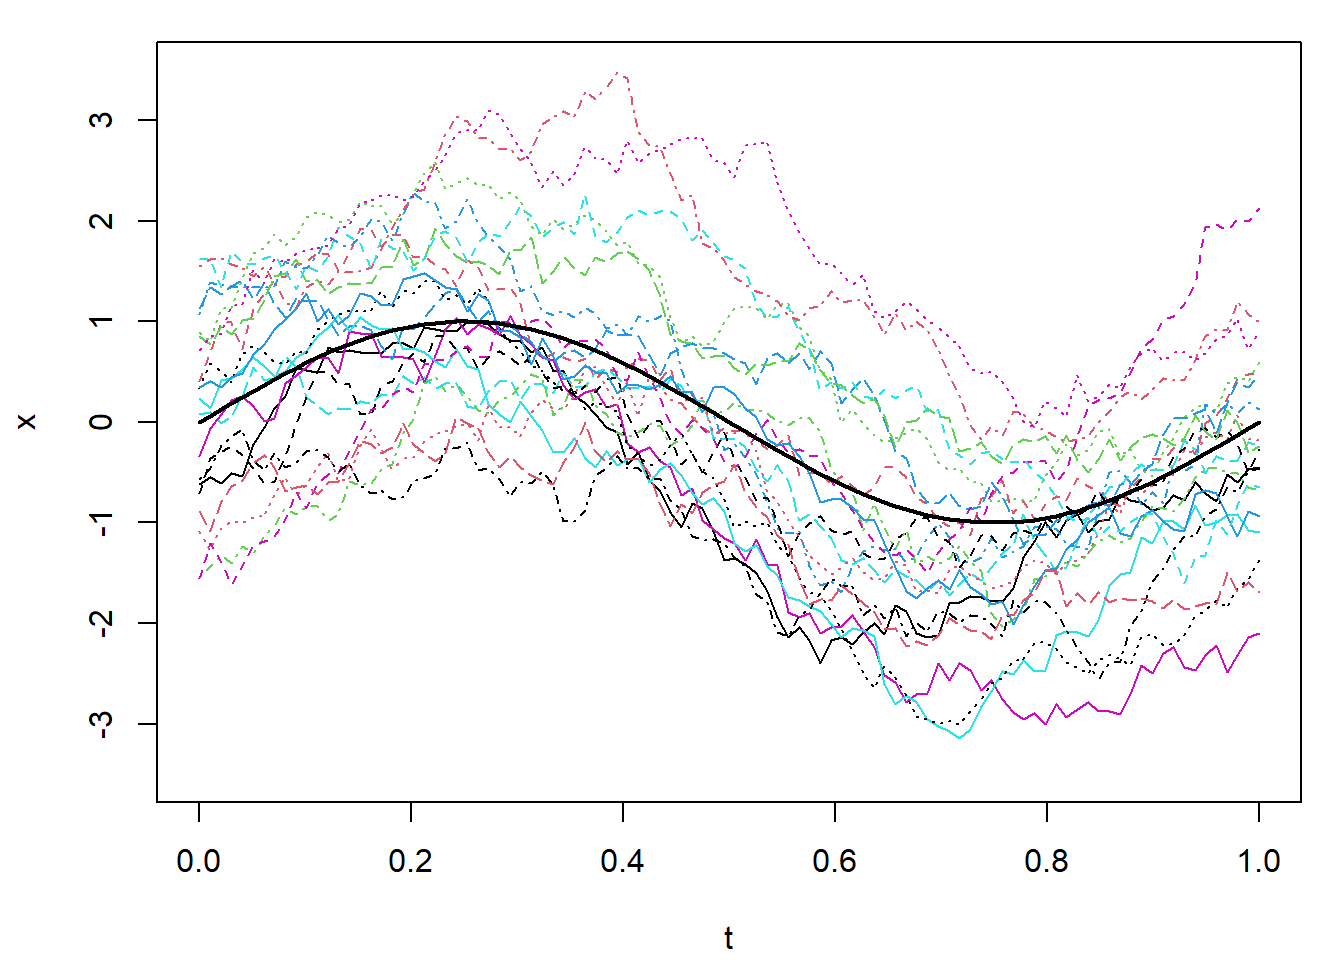
\includegraphics[width=0.7\linewidth]{07-Simulacion_multidimensional_files/figure-latex/funcional-plot-1} 

}

\caption{Realizaciones del proceso funcional del Ejemplo \ref{exm:funcional}, obtenidas a partir de la factorización de Cholesky.}\label{fig:funcional-plot}
\end{figure}

Alternativamente se podría emplear, por ejemplo, la funcion \texttt{mvrnorm}
del paquete \texttt{MASS} que emplea la factorización espectral (\texttt{eigen}) (y que tiene en cuenta una tolerancia relativa para correguir autovalores negativos próximos a cero):



\begin{Shaded}
\begin{Highlighting}[]
\KeywordTok{library}\NormalTok{(MASS)}
\NormalTok{mvrnorm}
\end{Highlighting}
\end{Shaded}

\begin{verbatim}
## function (n = 1, mu, Sigma, tol = 1e-06, empirical = FALSE, EISPACK = FALSE) 
## {
##     p <- length(mu)
##     if (!all(dim(Sigma) == c(p, p))) 
##         stop("incompatible arguments")
##     if (EISPACK) 
##         stop("'EISPACK' is no longer supported by R", domain = NA)
##     eS <- eigen(Sigma, symmetric = TRUE)
##     ev <- eS$values
##     if (!all(ev >= -tol * abs(ev[1L]))) 
##         stop("'Sigma' is not positive definite")
##     X <- matrix(rnorm(p * n), n)
##     if (empirical) {
##         X <- scale(X, TRUE, FALSE)
##         X <- X %*% svd(X, nu = 0)$v
##         X <- scale(X, FALSE, TRUE)
##     }
##     X <- drop(mu) + eS$vectors %*% diag(sqrt(pmax(ev, 0)), p) %*% 
##         t(X)
##     nm <- names(mu)
##     if (is.null(nm) && !is.null(dn <- dimnames(Sigma))) 
##         nm <- dn[[1L]]
##     dimnames(X) <- list(nm, NULL)
##     if (n == 1) 
##         drop(X)
##     else t(X)
## }
## <bytecode: 0x000000001588e090>
## <environment: namespace:MASS>
\end{verbatim}

\begin{Shaded}
\begin{Highlighting}[]
\NormalTok{x <-}\StringTok{ }\KeywordTok{mvrnorm}\NormalTok{(nsim, mu, x.cov)}

\KeywordTok{matplot}\NormalTok{(t, }\KeywordTok{t}\NormalTok{(x), }\DataTypeTok{type =} \StringTok{"l"}\NormalTok{)}
\KeywordTok{lines}\NormalTok{(t, mu, }\DataTypeTok{lwd =} \DecValTok{2}\NormalTok{)}
\end{Highlighting}
\end{Shaded}

\begin{figure}[!htb]

{\centering 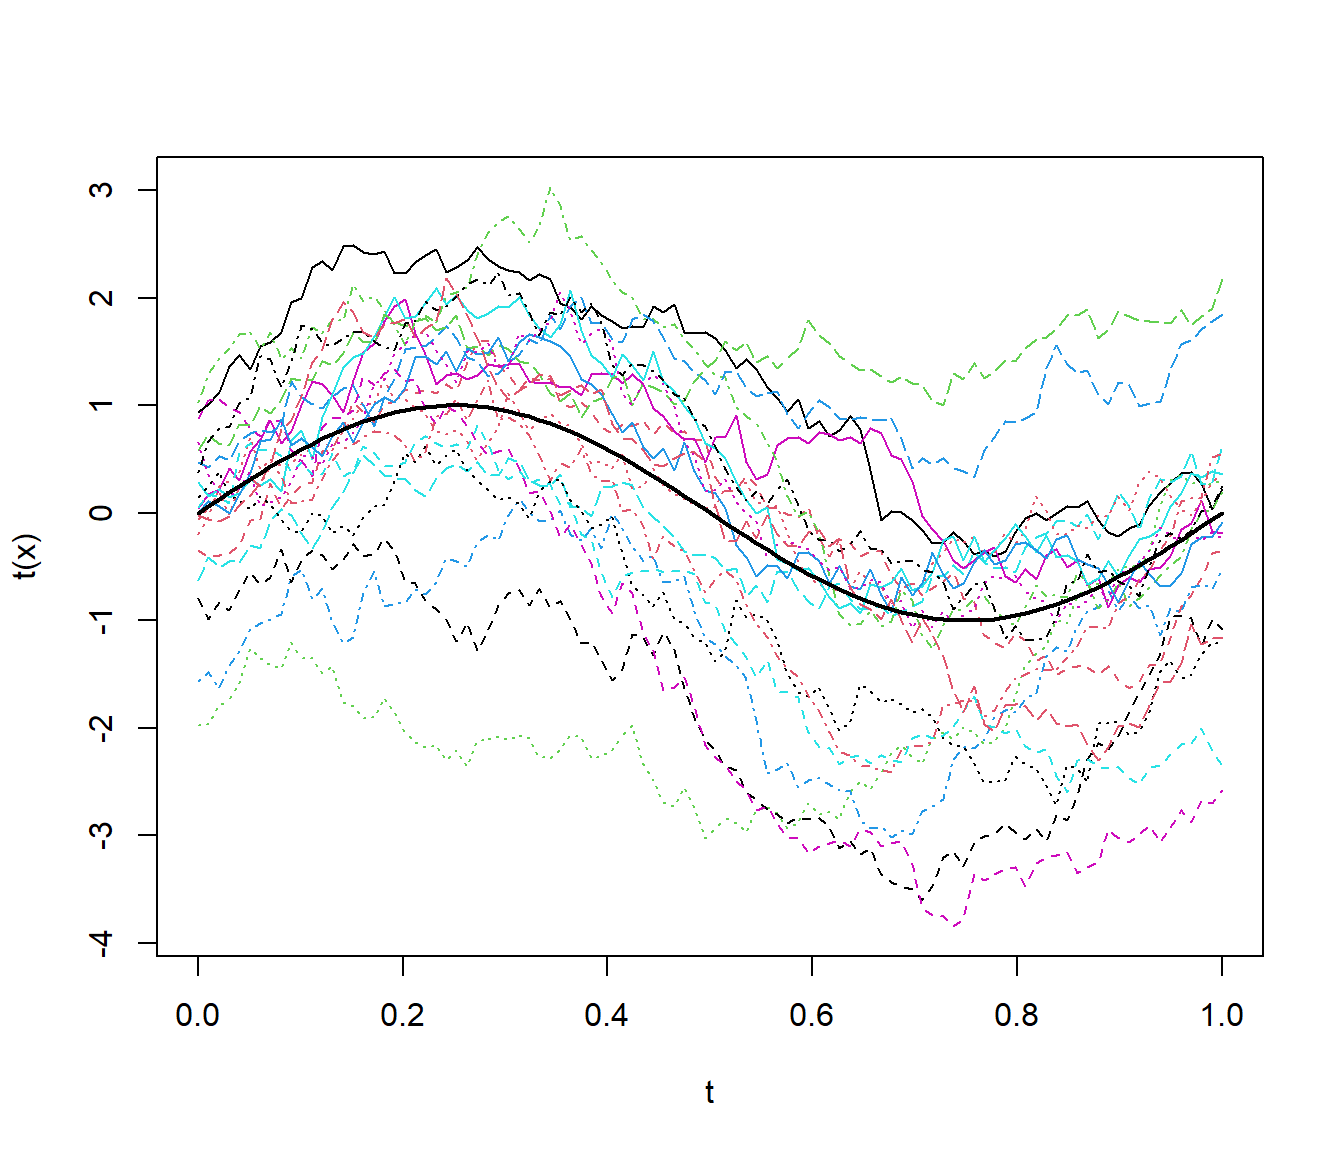
\includegraphics[width=0.7\linewidth]{07-Simulacion_multidimensional_files/figure-latex/funcional-plot2-1} 

}

\caption{Realizaciones del proceso funcional del Ejemplo \ref{exm:funcional}, obtenidas empleando la función \texttt{MASS::mvrnorm}.}\label{fig:funcional-plot2}
\end{figure}

Otros métodos para variables continuas relacionados con la factorización de la matriz de covarianzas son el método FFT (transformada rápida de Fourier; e.g.~Davies y Harte, 1987) o el \emph{Circular embedding} (Dietrich and Newsam, 1997), que realmente son el mismo.

\hypertarget{distrcond}{%
\section{Método de las distribuciones condicionadas}\label{distrcond}}

Teniendo en cuenta que:
\[f\left( x_1,x_2,\ldots,x_d\right)  =f_1\left( x_1\right)  \cdot
f_2\left( x_2|x_1\right)  \cdots f_d\left( x_d|x_1,x_2,\ldots,x_{d-1}\right),\]
donde las densidades condicionales pueden obtenerse a partir de las
correspondientes marginales:
\[f_i\left( x_i|x_1,x_2,\ldots,x_{i-1}\right)  =\frac{f_{1,\ldots
,i}\left( x_1,x_2,\ldots,x_i\right)  }{f_{1,\ldots,i-1}\left(
x_1,x_2,\ldots,x_{i-1}\right)},\]

se obtiene el siguiente algoritmo general:

\begin{conjecture}[de simulación mediante distribuciones condicionadas]
\protect\hypertarget{cnj:mult-distrcond}{}{\label{cnj:mult-distrcond} \iffalse (de simulación mediante distribuciones condicionadas) \fi{} }

\begin{enumerate}
\def\labelenumi{\arabic{enumi}.}
\item
  Generar \(X_1 \sim f_1\).
\item
  Desde \(i=2\) hasta \(d\) generar
  \(X_i \sim f_i\left( \cdot|X_1,X_2,\ldots,X_{i-1}\right)\).
\item
  Devolver \(\mathbf{X} =\left( X_1,X_2,\ldots,X_d\right)\).
\end{enumerate}
\end{conjecture}

\textbf{Nota}: En las simulaciones unidimensionales se puede tener en cuenta que
\(f_i\left( x_i|x_1,x_2,\ldots,x_{i-1}\right) \propto f_{1,\ldots,i}\left( x_1,x_2,\ldots,x_i\right)\).

\begin{example}[distribución uniforme en el círculo unitario]
\protect\hypertarget{exm:unnamed-chunk-8}{}{\label{exm:unnamed-chunk-8} \iffalse (distribución uniforme en el círculo unitario) \fi{} }
\end{example}

Se trata de la distribución bidimensional continua con densidad
constante en el círculo:
\[C = \left\{ \left( x_1, x_2 \right)  \in \mathbb{R}^2 : x_1^2 + x_2^2 \leq 1 \right\}.\]

Su función de densidad viene dada por:
\[f\left( x_1,x_2\right)  =\left\{
\begin{array}{ll}
\frac{1}{\pi} & \text{si } \left( x_1,x_2\right)  \in C\\
0 & \text{si } \left( x_1,x_2\right)  \notin C
\end{array}\right.\]

La densidad marginal de la primera variable resulta:
\[f_1\left( x_1\right)  =\int_{-\sqrt{1-x_1^2}}^{+\sqrt{1-x_1^2}}\frac{1}{\pi}dx_2
=\frac{2\sqrt{1-x_1^2}}{\pi}
\text{ si }x_1\in\left[-1,1\right],\]
es decir:
\[f_1\left( x_1\right)  =\left\{
\begin{array}{ll}
\frac{2}{\pi}\sqrt{1-x_1^2} & \text{si } x_1\in\left[  -1,1\right]  \\
0 & \text{si } x_1\notin\left[ -1,1\right]  
\end{array}\right.\]

Además:
\[f_2\left( x_2|x_1\right) = \frac{f\left( x_1,x_2\right)  }{f_1\left( x_1\right)} = \frac{\frac{1}{\pi}}{\frac{2\sqrt{1-x_1^2}}{\pi}}=\frac{1}{2\sqrt{1-x_1^2}}\text{, si }x_2\in\left[
-\sqrt{1-x_1^2},\sqrt{1-x_1^2}\right]\]
valiendo cero en otro caso.
Se tiene entonces que:
\[X_2|X_1 \sim \mathcal{U}\left(  -\sqrt{1-X_1^2},\sqrt{1-X_1^2}\right),\]
siempre que \(X_1\in\left[ -1,1\right]\).

Finalmente, el algoritmo resulta:

\begin{enumerate}
\def\labelenumi{\arabic{enumi}.}
\item
  Simular \(X_1\) con densidad \(f_1\left( x_1\right) =\frac{2}{\pi}\sqrt{1-x_1^2}1_{\{|x_1|\leq1\}}\).
\item
  Simular \(X_2\) con densidad \(\mathcal{U}\left( -\sqrt{1-X_1^2},\sqrt{1-X_1^2}\right)\).
\item
  Devolver \(\mathbf{X}=\left( X_1,X_2\right) ^t\).
\end{enumerate}

Para el paso 1 puede utilizarse, por ejemplo, el método de
aceptación/rechazo, pues se trata de una densidad acotada definida en un
intervalo acotado.

\begin{example}[distribución normal bidimensional]
\protect\hypertarget{exm:unnamed-chunk-9}{}{\label{exm:unnamed-chunk-9} \iffalse (distribución normal bidimensional) \fi{} }
\end{example}

En el caso de una distribución normal bidimensional:
\[\mathbf{X} = \begin{pmatrix}
 X_1 \\
 X_2
\end{pmatrix}  
\sim \mathcal{N} \left( \begin{pmatrix}
 \mu_1 \\
 \mu_2
\end{pmatrix} , 
\begin{pmatrix}
 \sigma^2_1 &  \sigma_1 \sigma_2 \rho \\
 \sigma_1 \sigma_2 \rho &  \sigma^2_2
\end{pmatrix} \right)\]

tendríamos que:

\[\begin{aligned}
f(x_1,x_2) &= \frac{1}{2 \pi \sigma_1 \sigma_2 \sqrt{1-\rho^2}} \\
&\exp \left( -\frac{1}{2 (1-\rho^2)} \left( \frac{(x_1 - \mu_1)^2}{\sigma_1^2} + \frac{(x_2 - \mu_2)^2}{\sigma_2^2} - \frac{2 \rho (x_1 - \mu_1) (x_2 - \mu_2)}{ \sigma_1 \sigma_2} \right)
\right)
\end{aligned}\]

de donde se deduce (ver e.g.~Cao, 2002, p.88; o ecuaciones \eqref{eq:mediacond} y \eqref{eq:varcond} en la Sección \ref{condnormal}) que:

\[f_1( x_1 ) = \frac{1}{\sigma_1\sqrt{2\pi}}
\exp\left( -\frac{(x_1 - \mu_1)^{2}}{2\sigma_1^{2}}\right)\]

\[\begin{aligned}
f_2\left( x_2|x_1\right)  &= \frac{f\left( x_1,x_2\right)  }{f_1\left( x_1\right)} \\ &= \frac{1}{\sigma_2\sqrt{2\pi (1-\rho^2)}}
\exp\left( -\frac{\left(x_2 - \mu_2 - \frac{\sigma_2}{\sigma_1}\rho( x_1 - \mu_1)\right)^{2}}{2\sigma_2^2 (1-\rho^2)}\right)
\end{aligned}\]

Por tanto:

\[\begin{aligned}
X_1 &\sim \mathcal{N}\left( \mu_1, \sigma_1^2 \right) \\
X_2 | X_1 &\sim \mathcal{N} \left( \mu_2 + \frac{\sigma_2}{\sigma_1}\rho( X_1 - \mu_1), \sigma_2^2 (1-\rho^2) \right)
\end{aligned}\]

y el algoritmo sería el siguiente:

\begin{conjecture}[de simulación de una normal bidimensional]
\protect\hypertarget{cnj:norm-bidim-cond}{}{\label{cnj:norm-bidim-cond} \iffalse (de simulación de una normal bidimensional) \fi{} }

\begin{enumerate}
\def\labelenumi{\arabic{enumi}.}
\item
  Simular \(Z_1, Z_2 \sim \mathcal{N}\left( 0, 1 \right)\) independientes.
\item
  Hacer \(X_1 = \mu_1 + \sigma_1 Z_1\).
\item
  Hacer \(X_2 =\mu_2 + \sigma_2 \rho Z_1 + \sigma_2 \sqrt{1-\rho^2} Z_2\).
\end{enumerate}
\end{conjecture}

Este algoritmo es el mismo que obtendríamos con la factorización de la matrix de covarianzas
ya que \(\Sigma = L L^t\) con:
\[L = \begin{pmatrix}
 \sigma^2_1 &  0 \\
 \sigma_2 \rho &  \sigma_2  \sqrt{1-\rho^2}
\end{pmatrix}\]

Además, esta aproximación puede generalizarse al caso multidimensional, ver Sección \ref{condnormal}.

\begin{exercise}
\protect\hypertarget{exr:cond2d}{}{\label{exr:cond2d} }
\end{exercise}

Considerando la variable aleatoria bidimensional del Ejemplo \ref{exm:ar-bidim} y teniendo en cuenta que la densidad marginal de la
variable \(X\) es:
\[f_{X}(x)=\left\{ 
\begin{array}{cl}
\frac{1}{8}\left( 5-3x^2\right)  & \text{si }x\in \lbrack -1,1] \\ 
0 & \text{en otro caso}
\end{array}
\right.\]
Describir brevemente un algoritmo para la simulación del
vector aleatorio basado en el método de las distribuciones
condicionadas (asumir que se dispone de un algoritmo para generar
observaciones de las distribuciones unidimensionales de interés).

\hypertarget{simulaciuxf3n-condicional-e-incondicional}{%
\section{Simulación condicional e incondicional}\label{simulaciuxf3n-condicional-e-incondicional}}

En ocasiones en inferencia estadística interesa la simulación condicional de nuevos valores de forma que se preserven los datos observados, para lo que se suele emplear el algoritmo anterior partiendo de la muestra observada:

\begin{conjecture}[de simulación condicional]
\protect\hypertarget{cnj:cond-incond}{}{\label{cnj:cond-incond} \iffalse (de simulación condicional) \fi{} }

\begin{enumerate}
\def\labelenumi{\arabic{enumi}.}
\item
  Obtener la distribución condicional (correspondiente al punto
  que se quiere simular) dada la muestra y los valores simulados
  anteriormente.
\item
  Simular un valor de la distribución condicional.
\item
  Agregar este valor al conjunto de datos y volver al paso 1.
\end{enumerate}
\end{conjecture}

En el caso de normalidad, en lugar de simular punto a punto,
podemos obtener fácilmente la distribución condicionada
para simular los valores de forma conjunta.

\hypertarget{condnormal}{%
\subsection{Simulación condicional de una normal multivariante}\label{condnormal}}

Si \(\mathbf{X} \sim \mathcal{N}_d\left( \boldsymbol\mu,\Sigma \right)\) es tal que \(\mathbf{X}\), \(\boldsymbol\mu\) y \(\boldsymbol\Sigma\) se particionan de la forma:
\[\mathbf{X} =
\begin{pmatrix}
 \mathbf{X}_1 \\
 \mathbf{X}_2
\end{pmatrix},  
\boldsymbol\mu =
\begin{pmatrix}
 \boldsymbol\mu_1 \\
 \boldsymbol\mu_2
\end{pmatrix}, 
\boldsymbol\Sigma =
\begin{pmatrix}
 \boldsymbol\Sigma_{11} & \boldsymbol\Sigma_{12} \\
 \boldsymbol\Sigma_{21} & \boldsymbol\Sigma_{22}
\end{pmatrix},\]
suponiendo que \(\mathbf{X}_1\) se corresponde con los valores observados y \(\mathbf{X}_2\) con los que se pretende simular,
entonces puede verse (e.g.~Ripley, 1987) que la distribución de \(\mathbf{X}_2 | \mathbf{X}_1\) es normal con:

\begin{equation}
E \left( \mathbf{X}_2 | \mathbf{X}_1 \right) = \boldsymbol\mu_2 + \boldsymbol\Sigma_{21} \boldsymbol\Sigma_{11}^{-1}
\left(  \mathbf{X}_1 - \boldsymbol\mu_1 \right), 
\label{eq:mediacond}
\end{equation}

\begin{equation}
Cov \left( \mathbf{X}_2 | \mathbf{X}_1 \right) =
\boldsymbol\Sigma_{22} - \boldsymbol\Sigma_{21} \boldsymbol\Sigma_{11}^{-1} \boldsymbol\Sigma_{12}.
\label{eq:varcond}
\end{equation}

\textbf{Nota}: La ecuación \eqref{eq:mediacond} coincide con la expresión de la predicción lineal óptima de \(\mathbf{X}_2\)
a partir de \(\mathbf{X}_1\) con media y varianzas conocidas (denominado predictor del kriging simple en estadística espacial, y la diagonal de \eqref{eq:varcond} son las correspondientes varianzas kriging).

\begin{example}[simulación condicional de datos funcionales o temporales]
\protect\hypertarget{exm:funcionalcond}{}{\label{exm:funcionalcond} \iffalse (simulación condicional de datos funcionales o temporales) \fi{} }
\end{example}

Continuando con el Ejemplo \ref{exm:funcional} anterior, consideramos los primeros
valores de una simulación incondicional como los datos:

\begin{Shaded}
\begin{Highlighting}[]
\NormalTok{idata <-}\StringTok{ }\NormalTok{t }\OperatorTok{<}\StringTok{ }\FloatTok{0.5}
\CommentTok{# idata <- t < 0.2 | t > 0.8}
\NormalTok{mu1 <-}\StringTok{ }\NormalTok{mu[idata]}
\NormalTok{n1 <-}\StringTok{ }\KeywordTok{length}\NormalTok{(mu1)}
\NormalTok{cov.data <-}\StringTok{ }\NormalTok{x.cov[idata, idata]}
\NormalTok{U <-}\StringTok{ }\KeywordTok{chol}\NormalTok{(cov.data)}
\CommentTok{# Simulación (incondicional):}
\KeywordTok{set.seed}\NormalTok{(}\DecValTok{1}\NormalTok{)}
\NormalTok{data <-}\StringTok{ }\KeywordTok{drop}\NormalTok{(mu1 }\OperatorTok{+}\StringTok{ }\KeywordTok{t}\NormalTok{(U) }\OperatorTok\StringTok{ }\KeywordTok{rnorm}\NormalTok{(n1))}
\end{Highlighting}
\end{Shaded}

Para obtener la simulación condicional en los puntos de predicción, calculamos la correspondiente media y matriz de covarianzas condicionadas:

\begin{Shaded}
\begin{Highlighting}[]
\NormalTok{mu2 <-}\StringTok{ }\NormalTok{mu[}\OperatorTok{!}\NormalTok{idata]}
\NormalTok{n2 <-}\StringTok{ }\KeywordTok{length}\NormalTok{(mu2)}
\NormalTok{cov.pred <-}\StringTok{ }\NormalTok{x.cov[}\OperatorTok{!}\NormalTok{idata, }\OperatorTok{!}\NormalTok{idata]}
\NormalTok{cov.preddat <-}\StringTok{ }\NormalTok{x.cov[}\OperatorTok{!}\NormalTok{idata, idata]}
\CommentTok{# Cálculo de los pesos kriging:}
\NormalTok{cov.data.inv <-}\StringTok{ }\KeywordTok{chol2inv}\NormalTok{(U)}
\NormalTok{lambda <-}\StringTok{ }\NormalTok{cov.preddat }\OperatorTok\StringTok{ }\NormalTok{cov.data.inv}
\CommentTok{# La media serán las predicciones del kriging simple:}
\NormalTok{kpred <-}\StringTok{ }\NormalTok{mu2 }\OperatorTok{+}\StringTok{ }\KeywordTok{drop}\NormalTok{(lambda }\OperatorTok\StringTok{ }\NormalTok{(data }\OperatorTok{-}\StringTok{ }\NormalTok{mu1))}
\CommentTok{# Varianza de la distribución condicional}
\NormalTok{kcov <-}\StringTok{ }\NormalTok{cov.pred }\OperatorTok{-}\StringTok{  }\NormalTok{lambda }\OperatorTok\StringTok{ }\KeywordTok{t}\NormalTok{(cov.preddat)}
\CommentTok{# (La diagonal serán las varianzas kriging). }
\end{Highlighting}
\end{Shaded}

Las simulaciones condicionales se obtendrán de forma análoga (Figura \ref{fig:funcional-cond}):



\begin{Shaded}
\begin{Highlighting}[]
\NormalTok{z <-}\StringTok{ }\KeywordTok{matrix}\NormalTok{(}\KeywordTok{rnorm}\NormalTok{(nsim }\OperatorTok{*}\StringTok{ }\NormalTok{n2), }\DataTypeTok{nrow =}\NormalTok{ n2)}
\NormalTok{y <-}\StringTok{ }\NormalTok{kpred }\OperatorTok{+}\StringTok{ }\KeywordTok{t}\NormalTok{(}\KeywordTok{chol}\NormalTok{(kcov)) }\OperatorTok\StringTok{ }\NormalTok{z}
\CommentTok{# Representación gráfica:}
\KeywordTok{plot}\NormalTok{(t, mu, }\DataTypeTok{type =} \StringTok{"l"}\NormalTok{, }\DataTypeTok{lwd =} \DecValTok{2}\NormalTok{, }\DataTypeTok{ylab =} \StringTok{"y"}\NormalTok{, }\DataTypeTok{ylim =} \KeywordTok{c}\NormalTok{(}\OperatorTok{-}\FloatTok{3.5}\NormalTok{, }\FloatTok{3.5}\NormalTok{)) }\CommentTok{# media teórica}
\KeywordTok{lines}\NormalTok{(t[idata], data) }\CommentTok{# datos}
\CommentTok{# y <- rep(NA, n)}
\CommentTok{# y[idata] <- data}
\CommentTok{# lines(t, y)}
\KeywordTok{matplot}\NormalTok{(t[}\OperatorTok{!}\NormalTok{idata], y, }\DataTypeTok{type =} \StringTok{"l"}\NormalTok{, }\DataTypeTok{add =} \OtherTok{TRUE}\NormalTok{) }\CommentTok{# simulaciones condicionales}
\KeywordTok{lines}\NormalTok{(t[}\OperatorTok{!}\NormalTok{idata], kpred, }\DataTypeTok{lwd =} \DecValTok{2}\NormalTok{, }\DataTypeTok{lty =} \DecValTok{2}\NormalTok{) }\CommentTok{# media condicional (predicción kriging)}
\end{Highlighting}
\end{Shaded}

\begin{figure}[!htb]

{\centering 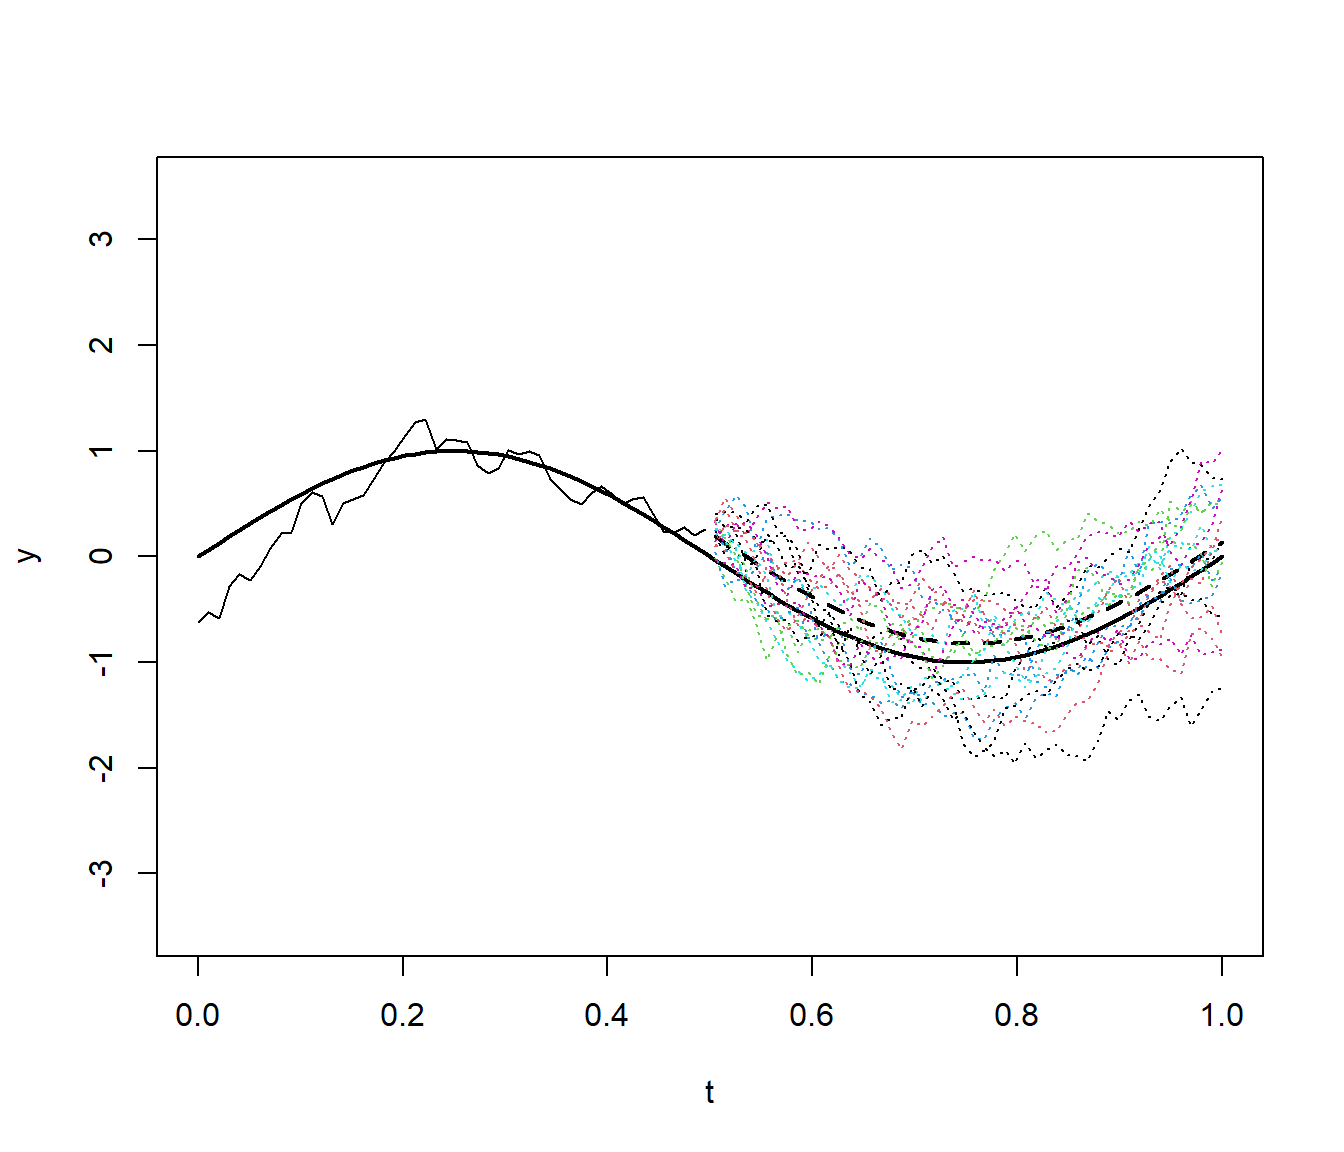
\includegraphics[width=0.7\linewidth]{07-Simulacion_multidimensional_files/figure-latex/funcional-cond-1} 

}

\caption{Realizaciones condicionales del proceso funcional del Ejemplo \ref{exm:funcionalcond}.}\label{fig:funcional-cond}
\end{figure}

\begin{example}[simulación condicional de datos espaciales]
\protect\hypertarget{exm:unnamed-chunk-12}{}{\label{exm:unnamed-chunk-12} \iffalse (simulación condicional de datos espaciales) \fi{} }
\end{example}

Consideramos un proceso espacial bidimensional normal
\(Z(\mathbf{s})\equiv Z(x,y)\) de media 0 y covariograma
exponencial:
\[Cov(Z(\mathbf{s}_1),Z(\mathbf{s}_2)) 
= C(\left\Vert \mathbf{s}_1-\mathbf{s}_2\right\Vert )
= e^{-\left\Vert \mathbf{s}_1-\mathbf{s}_2\right\Vert }.\]

En primer lugar, obtendremos una simulación del proceso en las posiciones
\(\left\{(0,0),(0,1),(1,0),(1,1)\right\}\) que será considerada posteriormente
como los datos observados.
Empleando las herramientas del paquete \texttt{geoR}, resulta muy fácil obtener
una simulación incondicional en una rejilla en el cuadrado unidad
mediante la función \texttt{grf}:

\begin{Shaded}
\begin{Highlighting}[]
\KeywordTok{library}\NormalTok{(geoR)}
\NormalTok{n <-}\StringTok{ }\DecValTok{4}
\KeywordTok{set.seed}\NormalTok{(}\DecValTok{1}\NormalTok{)}
\NormalTok{z <-}\StringTok{ }\KeywordTok{grf}\NormalTok{(n, }\DataTypeTok{grid =} \StringTok{"reg"}\NormalTok{, }\DataTypeTok{cov.pars =} \KeywordTok{c}\NormalTok{(}\DecValTok{1}\NormalTok{, }\DecValTok{1}\NormalTok{))}
\end{Highlighting}
\end{Shaded}

\begin{verbatim}
## grf: generating grid  2  *  2  with  4  points
## grf: process with  1  covariance structure(s)
## grf: nugget effect is: tausq= 0 
## grf: covariance model 1 is: exponential(sigmasq=1, phi=1)
## grf: decomposition algorithm used is:  cholesky 
## grf: End of simulation procedure. Number of realizations: 1
\end{verbatim}

\begin{Shaded}
\begin{Highlighting}[]
\CommentTok{# names(z)}
\NormalTok{z}\OperatorTok{$}\NormalTok{coords}
\end{Highlighting}
\end{Shaded}

\begin{verbatim}
##      x y
## [1,] 0 0
## [2,] 1 0
## [3,] 0 1
## [4,] 1 1
\end{verbatim}

\begin{Shaded}
\begin{Highlighting}[]
\NormalTok{z}\OperatorTok{$}\NormalTok{data}
\end{Highlighting}
\end{Shaded}

\begin{verbatim}
## [1] -0.62645381 -0.05969442 -0.98014198  1.09215113
\end{verbatim}

La \texttt{grf} función emplea por defecto el método de la factorización de la matriz de covarianzas,
sin embargo, si se desean obtener múltiples realizaciones, en lugar de llamar repetidamente a esta función (lo que implicaría factorizar repetidamente la matriz de covarianzas),
puede ser preferible emplear un código similar al siguiente (de forma que solo se realiza una vez dicha factorización, y suponiendo además que no es necesario conservar las distintas realizaciones):

\begin{Shaded}
\begin{Highlighting}[]
\CommentTok{# Posiciones datos}
\NormalTok{nx <-}\StringTok{ }\KeywordTok{c}\NormalTok{(}\DecValTok{2}\NormalTok{, }\DecValTok{2}\NormalTok{)}
\NormalTok{data.s <-}\StringTok{ }\KeywordTok{expand.grid}\NormalTok{(}\DataTypeTok{x =} \KeywordTok{seq}\NormalTok{(}\DecValTok{0}\NormalTok{, }\DecValTok{1}\NormalTok{, }\DataTypeTok{len =}\NormalTok{ nx[}\DecValTok{1}\NormalTok{]), }\DataTypeTok{y =} \KeywordTok{seq}\NormalTok{(}\DecValTok{0}\NormalTok{, }\DecValTok{1}\NormalTok{, }\DataTypeTok{len =}\NormalTok{ nx[}\DecValTok{2}\NormalTok{]))}
\CommentTok{# plot(data.s, type = "p", pch = 20, asp = 1) # Representar posiciones}

\CommentTok{# Matriz de varianzas covarianzas}
\NormalTok{cov.matrix <-}\StringTok{ }\KeywordTok{varcov.spatial}\NormalTok{(}\DataTypeTok{coords=}\NormalTok{data.s, }\DataTypeTok{cov.pars=}\KeywordTok{c}\NormalTok{(}\DecValTok{1}\NormalTok{,}\DecValTok{1}\NormalTok{))}\OperatorTok{$}\NormalTok{varcov}
\NormalTok{cov.matrix}
\end{Highlighting}
\end{Shaded}

\begin{verbatim}
##           [,1]      [,2]      [,3]      [,4]
## [1,] 1.0000000 0.3678794 0.3678794 0.2431167
## [2,] 0.3678794 1.0000000 0.2431167 0.3678794
## [3,] 0.3678794 0.2431167 1.0000000 0.3678794
## [4,] 0.2431167 0.3678794 0.3678794 1.0000000
\end{verbatim}

\begin{Shaded}
\begin{Highlighting}[]
\CommentTok{# Simular valores}
\KeywordTok{set.seed}\NormalTok{(}\DecValTok{1}\NormalTok{)}
\NormalTok{L <-}\StringTok{ }\KeywordTok{t}\NormalTok{(}\KeywordTok{chol}\NormalTok{(cov.matrix))}

\CommentTok{# Bucle simulación}
\NormalTok{nsim <-}\StringTok{ }\DecValTok{1} \CommentTok{# 1000}
\ControlFlowTok{for}\NormalTok{ (i }\ControlFlowTok{in} \DecValTok{1}\OperatorTok{:}\NormalTok{nsim) \{}
\NormalTok{  y <-}\StringTok{ }\NormalTok{L }\OperatorTok\StringTok{ }\KeywordTok{rnorm}\NormalTok{(n)}
  \CommentTok{# calcular estadísticos, errores,...}
\NormalTok{\}}
\NormalTok{y}
\end{Highlighting}
\end{Shaded}

\begin{verbatim}
##             [,1]
## [1,] -0.62645381
## [2,] -0.05969442
## [3,] -0.98014198
## [4,]  1.09215113
\end{verbatim}

Para generar simulaciones condicionales podemos emplear la función \texttt{krige.conv}.
Por ejemplo, para generar 4 simulaciones en la rejilla regular \(10\times10\) en el cuadrado unidad \([0,1] \times [0,1]\) condicionadas a los valores generados en el apartado anterior podríamos emplear el siguiente código:

\begin{Shaded}
\begin{Highlighting}[]
\CommentTok{# Posiciones simulación condicional}
\NormalTok{new.nx <-}\StringTok{ }\KeywordTok{c}\NormalTok{(}\DecValTok{20}\NormalTok{, }\DecValTok{20}\NormalTok{)}
\NormalTok{new.x <-}\StringTok{ }\KeywordTok{seq}\NormalTok{(}\DecValTok{0}\NormalTok{, }\DecValTok{1}\NormalTok{, }\DataTypeTok{len =}\NormalTok{ new.nx[}\DecValTok{1}\NormalTok{])}
\NormalTok{new.y <-}\StringTok{ }\KeywordTok{seq}\NormalTok{(}\DecValTok{0}\NormalTok{, }\DecValTok{1}\NormalTok{, }\DataTypeTok{len =}\NormalTok{ new.nx[}\DecValTok{2}\NormalTok{])}
\NormalTok{new.s <-}\StringTok{ }\KeywordTok{expand.grid}\NormalTok{(}\DataTypeTok{x =}\NormalTok{ new.x, }\DataTypeTok{y =}\NormalTok{ new.y)}
\KeywordTok{plot}\NormalTok{(data.s, }\DataTypeTok{type =} \StringTok{"p"}\NormalTok{, }\DataTypeTok{pch =} \DecValTok{20}\NormalTok{, }\DataTypeTok{asp =} \DecValTok{1}\NormalTok{)}
\KeywordTok{points}\NormalTok{(new.s)}
\end{Highlighting}
\end{Shaded}

\begin{figure}[!htb]

{\centering 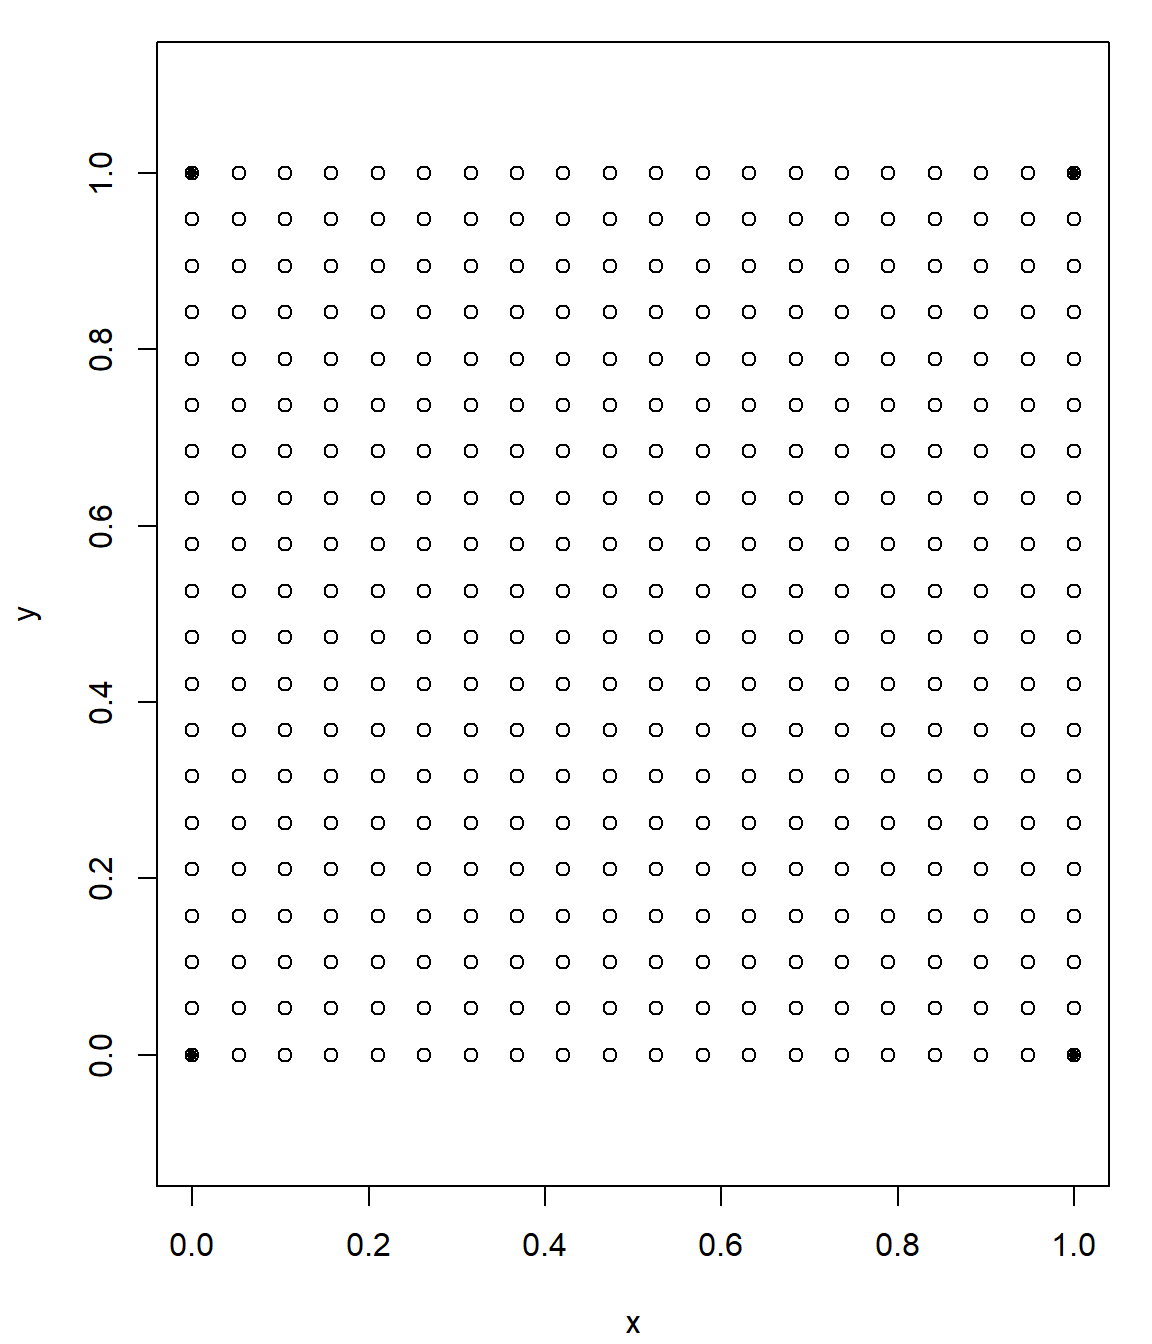
\includegraphics[width=0.7\linewidth]{07-Simulacion_multidimensional_files/figure-latex/pos-sp-simcond-1} 

}

\caption{Posiciones espaciales de las simulaciones condicionales (y las de los datos).}\label{fig:pos-sp-simcond}
\end{figure}

\begin{Shaded}
\begin{Highlighting}[]
\CommentTok{# Simulación condicional}
\KeywordTok{set.seed}\NormalTok{(}\DecValTok{1}\NormalTok{)}
\NormalTok{nsim.cond <-}\StringTok{ }\DecValTok{4}
\NormalTok{s.out <-}\StringTok{ }\KeywordTok{output.control}\NormalTok{(}\DataTypeTok{n.predictive =}\NormalTok{ nsim.cond)}
\NormalTok{kc <-}\StringTok{ }\KeywordTok{krige.conv}\NormalTok{(z, }\DataTypeTok{loc =}\NormalTok{ new.s, }\DataTypeTok{output =}\NormalTok{ s.out,}
                 \DataTypeTok{krige =} \KeywordTok{krige.control}\NormalTok{(}\DataTypeTok{type.krige=}\StringTok{"SK"}\NormalTok{, }\DataTypeTok{beta =} \DecValTok{0}\NormalTok{, }\DataTypeTok{cov.pars =} \KeywordTok{c}\NormalTok{(}\DecValTok{1}\NormalTok{, }\DecValTok{1}\NormalTok{)))}
\end{Highlighting}
\end{Shaded}

\begin{verbatim}
## krige.conv: results will be returned only for prediction locations inside the borders
## krige.conv: model with constant mean
## krige.conv: sampling from the predictive distribution (conditional simulations)
## krige.conv: Kriging performed using global neighbourhood
\end{verbatim}

Si las representamos podemos confirmar que los valores en las posiciones \(\left\{(0,0),(0,1),(1,0),(1,1)\right\}\) coinciden con los generados anteriormente.

\begin{Shaded}
\begin{Highlighting}[]
\CommentTok{# Generar gráficos}
\NormalTok{par.old <-}\StringTok{ }\KeywordTok{par}\NormalTok{(}\DataTypeTok{mfrow =} \KeywordTok{c}\NormalTok{(}\DecValTok{2}\NormalTok{, }\DecValTok{2}\NormalTok{), }\DataTypeTok{mar =} \KeywordTok{c}\NormalTok{(}\FloatTok{3.5}\NormalTok{, }\FloatTok{3.5}\NormalTok{, }\DecValTok{1}\NormalTok{, }\DecValTok{2}\NormalTok{), }\DataTypeTok{mgp =} \KeywordTok{c}\NormalTok{(}\FloatTok{1.5}\NormalTok{, }\FloatTok{.5}\NormalTok{, }\DecValTok{0}\NormalTok{))}
\NormalTok{zlim <-}\StringTok{ }\KeywordTok{range}\NormalTok{(kc}\OperatorTok{$}\NormalTok{simul)     }\CommentTok{# Escala común}
\CommentTok{# La versión actual de geoR::image.kriging() no admite múltiples gráficos en una ventana}
\CommentTok{# image(kc, val=kc$simul[,1], main="simul. cond. 1", zlim=zlim)}
\CommentTok{# image(kc, val=kc$simul[,2], main="simul. cond. 2", zlim=zlim)}
\CommentTok{# image(kc, val=kc$simul[,3], main="simul. cond. 3", zlim=zlim)}
\CommentTok{# image(kc, val=kc$simul[,4], main="simul. cond. 4", zlim=zlim)}
\KeywordTok{dim}\NormalTok{(kc}\OperatorTok{$}\NormalTok{simul) <-}\StringTok{ }\KeywordTok{c}\NormalTok{(new.nx, nsim.cond)}
\KeywordTok{image}\NormalTok{(new.x, new.y, kc}\OperatorTok{$}\NormalTok{simul[,,}\DecValTok{1}\NormalTok{], }\DataTypeTok{main=}\StringTok{"simul. cond. 1"}\NormalTok{,}
      \DataTypeTok{xlab =} \StringTok{"x"}\NormalTok{, }\DataTypeTok{ylab =} \StringTok{"y"}\NormalTok{, }\DataTypeTok{zlim =}\NormalTok{ zlim)}
\KeywordTok{image}\NormalTok{(new.x, new.y, kc}\OperatorTok{$}\NormalTok{simul[,,}\DecValTok{2}\NormalTok{], }\DataTypeTok{main=}\StringTok{"simul. cond. 2"}\NormalTok{,}
      \DataTypeTok{xlab =} \StringTok{"x"}\NormalTok{, }\DataTypeTok{ylab =} \StringTok{"y"}\NormalTok{, }\DataTypeTok{zlim =}\NormalTok{ zlim)}
\KeywordTok{image}\NormalTok{(new.x, new.y, kc}\OperatorTok{$}\NormalTok{simul[,,}\DecValTok{3}\NormalTok{], }\DataTypeTok{main=}\StringTok{"simul. cond. 3"}\NormalTok{,}
      \DataTypeTok{xlab =} \StringTok{"x"}\NormalTok{, }\DataTypeTok{ylab =} \StringTok{"y"}\NormalTok{, }\DataTypeTok{zlim =}\NormalTok{ zlim)}
\KeywordTok{image}\NormalTok{(new.x, new.y, kc}\OperatorTok{$}\NormalTok{simul[,,}\DecValTok{4}\NormalTok{], }\DataTypeTok{main=}\StringTok{"simul. cond. 4"}\NormalTok{,}
      \DataTypeTok{xlab =} \StringTok{"x"}\NormalTok{, }\DataTypeTok{ylab =} \StringTok{"y"}\NormalTok{, }\DataTypeTok{zlim =}\NormalTok{ zlim)}
\end{Highlighting}
\end{Shaded}

\begin{center}\includegraphics[width=0.9\linewidth]{07-Simulacion_multidimensional_files/figure-latex/unnamed-chunk-14-1} \end{center}

\begin{Shaded}
\begin{Highlighting}[]
\KeywordTok{par}\NormalTok{(par.old)}
\end{Highlighting}
\end{Shaded}

\hypertarget{simulaciuxf3n-condicional-a-partir-de-un-modelo-ajustado}{%
\subsection{Simulación condicional a partir de un modelo ajustado}\label{simulaciuxf3n-condicional-a-partir-de-un-modelo-ajustado}}

En la práctica normalmente se ajusta un modelo a los datos observados y posteriormente se obtienen las simulaciones condicionadas empleando el modelo ajustado.

En \texttt{R} se incluye una función genérica\footnote{Se pueden implementar métodos específicos para cada tipo (clase) de objeto; en este caso para cada tipo de modelo ajustado y podemos mostrar los disponibles mediante el comando \texttt{methods(simulate)}.} \texttt{simulate()} que permite generar respuestas a partir de modelos ajustados (siempre que esté implementado el método correspondiente al tipo de modelo).
Los métodos para modelos lineales y modelos lineales generalizamos están implementados en el paquete base \texttt{stats}.
Muchos otros paquetes que proporcionan modelos adicionales, implementan también los correspondientes métodos \texttt{simulate()}.
Por ejemplo, en el caso de series de tiempo, el paquete \texttt{forecast} permite ajustar distintos tipos de modelos y generar simulaciones a partir de ellos:

\begin{Shaded}
\begin{Highlighting}[]
\KeywordTok{library}\NormalTok{(forecast)}
\NormalTok{data <-}\StringTok{ }\KeywordTok{window}\NormalTok{(co2, }\DecValTok{1990}\NormalTok{) }\CommentTok{# datos de co2 desde 1990}
\KeywordTok{plot}\NormalTok{(data, }\DataTypeTok{ylab =} \KeywordTok{expression}\NormalTok{(}\StringTok{"Atmospheric concentration of CO"}\NormalTok{[}\DecValTok{2}\NormalTok{]),}
     \DataTypeTok{xlim =} \KeywordTok{c}\NormalTok{(}\DecValTok{1990}\NormalTok{, }\DecValTok{2000}\NormalTok{), }\DataTypeTok{ylim =} \KeywordTok{c}\NormalTok{(}\DecValTok{350}\NormalTok{, }\DecValTok{375}\NormalTok{))}
\end{Highlighting}
\end{Shaded}

\begin{center}\includegraphics[width=0.7\linewidth]{07-Simulacion_multidimensional_files/figure-latex/unnamed-chunk-15-1} \end{center}

\begin{Shaded}
\begin{Highlighting}[]
\CommentTok{# Se podrían ajustar distintos tipos de modelos}
\NormalTok{fit <-}\StringTok{ }\KeywordTok{ets}\NormalTok{(data)}
\CommentTok{# fit <- auto.arima(data)}
\end{Highlighting}
\end{Shaded}

Podemos obtener predicciones (media de la distribución condicional) e intervalos de predicción:

\begin{Shaded}
\begin{Highlighting}[]
\NormalTok{pred <-}\StringTok{ }\KeywordTok{forecast}\NormalTok{(fit, }\DataTypeTok{h =} \DecValTok{24}\NormalTok{, }\DataTypeTok{level =} \DecValTok{95}\NormalTok{)}
\NormalTok{pred}
\end{Highlighting}
\end{Shaded}

\begin{verbatim}
##          Point Forecast    Lo 95    Hi 95
## Jan 1998       365.1118 364.5342 365.6894
## Feb 1998       366.1195 365.4572 366.7819
## Mar 1998       367.0161 366.2786 367.7535
## Apr 1998       368.2749 367.4693 369.0806
## May 1998       368.9282 368.0596 369.7968
## Jun 1998       368.2240 367.2967 369.1513
## Jul 1998       366.5823 365.5997 367.5649
## Aug 1998       364.4895 363.4546 365.5244
## Sep 1998       362.6586 361.5738 363.7434
## Oct 1998       362.7805 361.6479 363.9130
## Nov 1998       364.2045 363.0262 365.3829
## Dec 1998       365.5250 364.3025 366.7476
## Jan 1999       366.6002 365.3349 367.8654
## Feb 1999       367.6078 366.3013 368.9144
## Mar 1999       368.5044 367.1578 369.8510
## Apr 1999       369.7633 368.3777 371.1488
## May 1999       370.4165 368.9930 371.8400
## Jun 1999       369.7124 368.2519 371.1728
## Jul 1999       368.0706 366.5741 369.5671
## Aug 1999       365.9778 364.4461 367.5096
## Sep 1999       364.1469 362.5806 365.7131
## Oct 1999       364.2688 362.6688 365.8688
## Nov 1999       365.6929 364.0597 367.3260
## Dec 1999       367.0134 365.3477 368.6790
\end{verbatim}

Para análisis adicionales nos puede interesar generar simulaciones (por defecto de la distribución condicional, \texttt{future\ =\ TRUE}):

\begin{Shaded}
\begin{Highlighting}[]
\KeywordTok{set.seed}\NormalTok{(}\DecValTok{321}\NormalTok{)}
\NormalTok{sim.cond <-}\StringTok{ }\KeywordTok{simulate}\NormalTok{(fit, }\DecValTok{24}\NormalTok{)}

\KeywordTok{plot}\NormalTok{(pred)}
\KeywordTok{lines}\NormalTok{(sim.cond, }\DataTypeTok{lwd =} \DecValTok{2}\NormalTok{, }\DataTypeTok{col =} \StringTok{"red"}\NormalTok{)}
\end{Highlighting}
\end{Shaded}

\begin{figure}[!htb]

{\centering \includegraphics[width=0.7\linewidth]{07-Simulacion_multidimensional_files/figure-latex/simulate-forecast-1} 

}

\caption{Ejemplo de una serie de tiempo (datos observados de co2 en el observatorio Mauna Loa), predicciones futuras (en azul; media distribución condicional) y simulación condicional (en rojo) obtenidas a partir de un modelo ajustado.}\label{fig:simulate-forecast}
\end{figure}

Para más detalles ver Hyndman y Athanasopoulos (2018, secciones \href{https://otexts.com/fpp2/prediction-intervals.html}{4.3} y \href{https://otexts.com/fpp2/bootstrap.html}{11.4}).

\hypertarget{simulaciuxf3n-basada-en-cuxf3pulas}{%
\section{Simulación basada en cópulas}\label{simulaciuxf3n-basada-en-cuxf3pulas}}

Una cópula es una función de distribución multidimensional con distribuciones marginales uniformes (e.g.~Nelsen, 2006; Hofert, 2018).
Se emplean principalmente para la construcción de distribuciones multivariantes a partir de distribuciones marginales (también en análisis de dependencia y medidas de asociación).

Por simplicidad nos centraremos en el caso bidimensional.
El teorema central en la teoría de cópulas es el teorema de Sklar (1959), que en este caso es:

\begin{theorem}[de Sklar, caso bidimensional]
\protect\hypertarget{thm:sklar}{}{\label{thm:sklar} \iffalse (de Sklar, caso bidimensional) \fi{} }

Si \((X,Y)\) es una variable aleatoria bidimensional con función de distribución conjunta \(F(\cdot,\cdot)\) y distribuciones marginales \(F_1(\cdot)\) y \(F_2(\cdot)\) respectivamente, entonces existe una cópula \(C(\cdot,\cdot)\) tal que:
\[F(x,y)=C\left( F_1(x),F_2(y)\right) ,\quad \forall x,y\in\mathbb{R}.\]
Además, si \(F_1(\cdot)\) y \(F_2(\cdot)\) son continuas entonces \(C(\cdot,\cdot)\) es única.
Siendo el recíproco también cierto.
\end{theorem}

\hypertarget{cuxf3pulas-arquimedianas}{%
\subsection{Cópulas Arquimedianas}\label{cuxf3pulas-arquimedianas}}

Además de las cópulas Gausianas, es una de las familias de cópulas más utilizadas.
Son de la forma:
\[C(x_1,x_2,\dots,x_d)
=\Psi^{-1}\left( \sum_{i=1}^d\Psi\left( F_i(x_i)\right)\right),\]
siendo \(\Psi\) su función generadora.

Una condición suficiente para que sea una cópula multidimensional válida es que \(\Psi(1)=0\), \(\lim \limits_{x\ \rightarrow0}\Psi(x)=\infty\), \(\Psi^{\prime}(x)<0\) y \(\Psi^{\prime \prime}(x)>0\).

\textbf{Ejemplos}:

\begin{itemize}
\item
  Cópula producto o independiente:
  \(\Psi(x)=-\ln(x)\),
  \[F(x,y)=F_1(x)F_2(y).\]
\item
  Cópula de Clayton: \(\Psi(x)=\frac{1}{\alpha}\left( x^{-\alpha }-1\right) ;\alpha>0\),
  \[F(x,y)=(F_1(x)^{-\alpha}+F_2(y)^{-\alpha}-1)^{-1/\alpha}.\]
\item
  Cópula de Gumbel:
  \(\Psi(x)=\left( -\ln(x)\right)^{\alpha};\alpha \geq1\)
\end{itemize}

\hypertarget{simulaciuxf3n}{%
\subsection{Simulación}\label{simulaciuxf3n}}

Las cópulas pueden facilitar notablemente la simulación de la distribución conjunta.
Si \((U,V)\sim C(\cdot,\cdot)\) (marginales uniformes):
\[\left( F_1^{-1}(U),F_2^{-1}(V)\right)  \sim F(\cdot,\cdot)\]

En la mayoría de los casos se dispone de expresiones explicitas de \(C_{u}(v)\equiv C_2\left( \left. v\right \vert u\right)\) y de su inversa \(C_{u}^{-1}(w)\), por lo que se puede generar \((U,V)\) fácilmente mediante el método secuencial de distribuciones condicionadas descrito en la Sección \ref{distrcond}.

\begin{conjecture}[de simulación bidimensional mediante cópulas]
\protect\hypertarget{cnj:copula-bidim}{}{\label{cnj:copula-bidim} \iffalse (de simulación bidimensional mediante cópulas) \fi{} }

\begin{enumerate}
\def\labelenumi{\arabic{enumi}.}
\item
  Generar \(U,W\sim \mathcal{U}(0,1)\)
\item
  Obtener \(V=C_{U}^{-1}(W)\)
\item
  Devolver \(\left( F_1^{-1}(U),F_2^{-1}(V)\right)\)
\end{enumerate}
\end{conjecture}

\begin{exercise}[Cópula bidimensional de Clayton]
\protect\hypertarget{exr:clayton2d}{}{\label{exr:clayton2d} \iffalse (Cópula bidimensional de Clayton) \fi{} }
\end{exercise}

Consideramos una variable aleatoria bidimensional con distribuciones marginales uniformes y distribución bidimensional determinada por la cópula de Clayton.

\begin{enumerate}
\def\labelenumi{\alph{enumi})}
\item
  Teniendo en cuenta que en este caso:
  \[C_{u}^{-1}(w)\equiv\left(  u^{-\alpha}\left(  
  w^{-\frac{\alpha}{\alpha+1}}-1\right) + 1 \right)^{-\frac{1}{\alpha}},\]
  diseñar una rutina que permita generar una muestra de tamaño \(n\)
  de esta distribución.

\begin{Shaded}
\begin{Highlighting}[]
\NormalTok{rcclayton <-}\StringTok{ }\ControlFlowTok{function}\NormalTok{(alpha, n) \{}
\NormalTok{  val <-}\StringTok{ }\KeywordTok{cbind}\NormalTok{(}\KeywordTok{runif}\NormalTok{(n), }\KeywordTok{runif}\NormalTok{(n))}
\NormalTok{  val[, }\DecValTok{2}\NormalTok{] <-}\StringTok{ }\NormalTok{(val[, }\DecValTok{1}\NormalTok{]}\OperatorTok{^}\NormalTok{(}\OperatorTok{-}\NormalTok{alpha) }\OperatorTok{*}\StringTok{ }
\StringTok{              }\NormalTok{(val[, }\DecValTok{2}\NormalTok{]}\OperatorTok{^}\NormalTok{(}\OperatorTok{-}\NormalTok{alpha}\OperatorTok{/}\NormalTok{(alpha }\OperatorTok{+}\StringTok{ }\DecValTok{1}\NormalTok{)) }\OperatorTok{-}\StringTok{ }\DecValTok{1}\NormalTok{) }\OperatorTok{+}\StringTok{ }\DecValTok{1}\NormalTok{)}\OperatorTok{^}\NormalTok{(}\OperatorTok{-}\DecValTok{1}\OperatorTok{/}\NormalTok{alpha)}
  \KeywordTok{return}\NormalTok{(val)}
\NormalTok{\}}
\end{Highlighting}
\end{Shaded}
\item
  Utilizando la rutina anterior generar una muestra de tamaño
  10000 y representar gráficamente los valores obtenidos y sus
  distribuciones marginales.

\begin{Shaded}
\begin{Highlighting}[]
\KeywordTok{set.seed}\NormalTok{(}\DecValTok{54321}\NormalTok{)}
\NormalTok{rcunif <-}\StringTok{ }\KeywordTok{rcclayton}\NormalTok{(}\DecValTok{2}\NormalTok{,}\DecValTok{10000}\NormalTok{)}
\KeywordTok{plot}\NormalTok{(rcunif, }\DataTypeTok{xlab =} \StringTok{"u"}\NormalTok{, }\DataTypeTok{ylab =} \StringTok{"v"}\NormalTok{)}
\end{Highlighting}
\end{Shaded}

  \begin{figure}[!htb]

  {\centering \includegraphics[width=0.7\linewidth]{07-Simulacion_multidimensional_files/figure-latex/cclayton2-dispersion-1} 

  }

  \caption{Gráfico de dispersión de los valores generados con distribución bidimensional de Clayton.}\label{fig:cclayton2-dispersion}
  \end{figure}

  Representar la densidad conjunta (con \texttt{sm::sm.density()}) y las marginales {[}Figuras: \ref{fig:cclayton2b-dispersion}, \ref{fig:cclayton3-dispersion}{]}:

\begin{Shaded}
\begin{Highlighting}[]
\CommentTok{# Densidad conjunta}
\CommentTok{# if(!require(sm)) stop('Required pakage `sm` not installed.')}
\NormalTok{sm}\OperatorTok{::}\KeywordTok{sm.density}\NormalTok{(rcunif, }\DataTypeTok{xlab =} \StringTok{"u"}\NormalTok{, }\DataTypeTok{ylab =} \StringTok{"v"}\NormalTok{, }\DataTypeTok{zlab =} \StringTok{"Density"}\NormalTok{)    }
\end{Highlighting}
\end{Shaded}

\begin{verbatim}
## Warning: weights overwritten by binning
\end{verbatim}

  \begin{figure}[!htb]

  {\centering \includegraphics[width=0.7\linewidth]{07-Simulacion_multidimensional_files/figure-latex/cclayton2-conjunta-1} 

  }

  \caption{Densidad conjunta de los valores generados con distribución bidimensional de Clayton.}\label{fig:cclayton2-conjunta}
  \end{figure}

\begin{Shaded}
\begin{Highlighting}[]
\CommentTok{# Distribuciones marginales}
\NormalTok{par.old <-}\StringTok{ }\KeywordTok{par}\NormalTok{(}\DataTypeTok{mfrow =} \KeywordTok{c}\NormalTok{(}\DecValTok{1}\NormalTok{, }\DecValTok{2}\NormalTok{))}
\KeywordTok{hist}\NormalTok{(rcunif[,}\DecValTok{1}\NormalTok{], }\DataTypeTok{freq =} \OtherTok{FALSE}\NormalTok{, }\DataTypeTok{xlab =} \StringTok{"u"}\NormalTok{)}
\KeywordTok{abline}\NormalTok{(}\DataTypeTok{h =} \DecValTok{1}\NormalTok{)}
\KeywordTok{hist}\NormalTok{(rcunif[,}\DecValTok{2}\NormalTok{], }\DataTypeTok{freq =} \OtherTok{FALSE}\NormalTok{, }\DataTypeTok{xlab =} \StringTok{"v"}\NormalTok{)}
\KeywordTok{abline}\NormalTok{(}\DataTypeTok{h =} \DecValTok{1}\NormalTok{)}
\end{Highlighting}
\end{Shaded}

  \begin{figure}[!htb]

  {\centering \includegraphics[width=0.9\linewidth]{07-Simulacion_multidimensional_files/figure-latex/cclayton2-marginales-1} 

  }

  \caption{Distribuciones marginales de los valores generados con distribución bidimensional de Clayton.}\label{fig:cclayton2-marginales}
  \end{figure}

\begin{Shaded}
\begin{Highlighting}[]
\KeywordTok{par}\NormalTok{(par.old)}
\end{Highlighting}
\end{Shaded}

  Empleando el paquete \emph{copula} {[}Figuras: \ref{fig:cclayton2b-dispersion}, \ref{fig:cclayton3-dispersion}{]}:

\begin{Shaded}
\begin{Highlighting}[]
\ControlFlowTok{if}\NormalTok{(}\OperatorTok{!}\KeywordTok{require}\NormalTok{(copula)) }\KeywordTok{stop}\NormalTok{(}\StringTok{'Required pakage `copula` not installed.'}\NormalTok{)}
\NormalTok{clayton.cop <-}\StringTok{ }\KeywordTok{claytonCopula}\NormalTok{(}\DecValTok{2}\NormalTok{, }\DataTypeTok{dim =} \DecValTok{2}\NormalTok{) }\CommentTok{# caso bidimensional}
\NormalTok{y <-}\StringTok{ }\KeywordTok{rCopula}\NormalTok{(}\DecValTok{10000}\NormalTok{, clayton.cop)}
\KeywordTok{plot}\NormalTok{(y, }\DataTypeTok{xlab =} \StringTok{"u"}\NormalTok{, }\DataTypeTok{ylab =} \StringTok{"v"}\NormalTok{)}
\end{Highlighting}
\end{Shaded}

  \begin{figure}[!htb]

  {\centering \includegraphics[width=0.7\linewidth]{07-Simulacion_multidimensional_files/figure-latex/cclayton2b-dispersion-1} 

  }

  \caption{Gráfico de dispersión de los valores generados con distribución bidimensional de Clayton empleando el paquete `copula`.}\label{fig:cclayton2b-dispersion}
  \end{figure}

\begin{Shaded}
\begin{Highlighting}[]
\NormalTok{clayton.cop <-}\StringTok{ }\KeywordTok{claytonCopula}\NormalTok{(}\DecValTok{2}\NormalTok{, }\DataTypeTok{dim =} \DecValTok{3}\NormalTok{) }\CommentTok{# caso tridimensional}
\NormalTok{y <-}\StringTok{ }\KeywordTok{rCopula}\NormalTok{(}\DecValTok{10000}\NormalTok{, clayton.cop)}
\CommentTok{# scatterplot3d::scatterplot3d(y)}
\NormalTok{plot3D}\OperatorTok{:::}\KeywordTok{points3D}\NormalTok{(y[,}\DecValTok{1}\NormalTok{], y[,}\DecValTok{2}\NormalTok{], y[, }\DecValTok{3}\NormalTok{], }\DataTypeTok{colvar =} \OtherTok{NULL}\NormalTok{, }
                  \DataTypeTok{xlab =} \StringTok{"u1"}\NormalTok{, }\DataTypeTok{ylab =} \StringTok{"u2"}\NormalTok{, }\DataTypeTok{zlab =} \StringTok{"u3"}\NormalTok{) }
\end{Highlighting}
\end{Shaded}

  \begin{figure}[!htb]

  {\centering \includegraphics[width=0.7\linewidth]{07-Simulacion_multidimensional_files/figure-latex/cclayton3-dispersion-1} 

  }

  \caption{Gráfico de dispersión de los valores generados con distribución trididimensional de Clayton empleando el paquete `copula`.}\label{fig:cclayton3-dispersion}
  \end{figure}
\item
  A partir de la muestra anterior generar una muestra de una v.a.
  bidimensional con distribuciones marginales exponenciales de
  parámetros 1 y 2 respectivamente (y distribución bidimensional
  determinada por la cópula de Clayton).

\begin{Shaded}
\begin{Highlighting}[]
\NormalTok{rcexp <-}\StringTok{ }\KeywordTok{cbind}\NormalTok{(}\KeywordTok{qexp}\NormalTok{(rcunif[,}\DecValTok{1}\NormalTok{], }\DecValTok{1}\NormalTok{), }\KeywordTok{qexp}\NormalTok{(rcunif[,}\DecValTok{2}\NormalTok{], }\DecValTok{2}\NormalTok{))}
\KeywordTok{plot}\NormalTok{(rcexp, }\DataTypeTok{xlab =} \StringTok{"exp1"}\NormalTok{, }\DataTypeTok{ylab =} \StringTok{"exp2"}\NormalTok{)  }
\end{Highlighting}
\end{Shaded}

  \begin{figure}[!htb]

  {\centering \includegraphics[width=0.7\linewidth]{07-Simulacion_multidimensional_files/figure-latex/cclayton-exp-conjunta-1} 

  }

  \caption{Gráfico de dispersión de los valores generados con distribución exponencial y dependencia definida por la cópula de Clayton.}\label{fig:cclayton-exp-conjunta}
  \end{figure}

\begin{Shaded}
\begin{Highlighting}[]
\CommentTok{# Distribuciones marginales}
\NormalTok{par.old <-}\StringTok{ }\KeywordTok{par}\NormalTok{(}\DataTypeTok{mfrow =} \KeywordTok{c}\NormalTok{(}\DecValTok{1}\NormalTok{, }\DecValTok{2}\NormalTok{))}
\KeywordTok{hist}\NormalTok{(rcexp[,}\DecValTok{1}\NormalTok{], }\DataTypeTok{freq =} \OtherTok{FALSE}\NormalTok{, }\DataTypeTok{xlab =} \StringTok{"exp1"}\NormalTok{)}
\KeywordTok{curve}\NormalTok{(}\KeywordTok{dexp}\NormalTok{(x, }\DecValTok{1}\NormalTok{), }\DataTypeTok{add =} \OtherTok{TRUE}\NormalTok{)}
\KeywordTok{hist}\NormalTok{(rcexp[,}\DecValTok{2}\NormalTok{], }\DataTypeTok{freq =} \OtherTok{FALSE}\NormalTok{, }\DataTypeTok{xlab =} \StringTok{"exp2"}\NormalTok{)}
\KeywordTok{curve}\NormalTok{(}\KeywordTok{dexp}\NormalTok{(x, }\DecValTok{2}\NormalTok{), }\DataTypeTok{add =} \OtherTok{TRUE}\NormalTok{)}
\end{Highlighting}
\end{Shaded}

  \begin{figure}[!htb]

  {\centering \includegraphics[width=0.9\linewidth]{07-Simulacion_multidimensional_files/figure-latex/cclayton-exp-marginales-1} 

  }

  \caption{Distribuciones marginales exponenciales de los valores generados con dependencia definida por la cópula de Clayton.}\label{fig:cclayton-exp-marginales}
  \end{figure}

\begin{Shaded}
\begin{Highlighting}[]
\KeywordTok{par}\NormalTok{(par.old)}
\end{Highlighting}
\end{Shaded}
\end{enumerate}

\hypertarget{mult-discr}{%
\section{Simulación de distribuciones multivariantes discretas}\label{mult-discr}}

\hypertarget{muxe9todos-de-codificaciuxf3n-o-etiquetado-para-variables-discretas}{%
\subsection{Métodos de codificación o etiquetado para variables discretas}\label{muxe9todos-de-codificaciuxf3n-o-etiquetado-para-variables-discretas}}

En el caso de una distribución \(d\)-dimensional discreta el procedimiento habitual es simular una variable aleatoria discreta unidimensional equivalente.
Este tipo de procedimientos son conocidos como métodos de etiquetado o codificación y la idea básica consistiría en construir un
indice unidimensional equivalente al indice multidimensional,
mediante una función de etiquetado
\(l(\mathbf{i}) = l\left(i_1, i_2, \ldots,i_d \right) \in \mathbb{N}\).

Si la variable discreta multidimensional tiene soporte finito, este tipo de recodificación se puede hacer de forma automática en \texttt{R} cambiando simplemente el indexado\footnote{En \texttt{R} podemos obtener el índice multidimensional empleando la función \texttt{arrayInd(ind,\ .dim,\ ...)}, siendo \texttt{ind} un vector de índices unidimensionales.} (empleando la función \texttt{as.vector()} para cambiar a un indexado unidimensional y posteriormente las funciones \texttt{as.matrix()}, o \texttt{as.array()}, para reconstruir el indexado multidimensional).

Como ejemplo ilustrativo (en el caso bidimensional) podríamos emplear el siguiente código:

\begin{Shaded}
\begin{Highlighting}[]
\NormalTok{z <-}\StringTok{ }\DecValTok{11}\OperatorTok{:}\DecValTok{18}
\NormalTok{xy <-}\StringTok{ }\KeywordTok{matrix}\NormalTok{(z, }\DataTypeTok{ncol =} \DecValTok{2}\NormalTok{)}
\NormalTok{xy}
\end{Highlighting}
\end{Shaded}

\begin{verbatim}
##      [,1] [,2]
## [1,]   11   15
## [2,]   12   16
## [3,]   13   17
## [4,]   14   18
\end{verbatim}

\begin{Shaded}
\begin{Highlighting}[]
\NormalTok{z <-}\StringTok{ }\KeywordTok{as.vector}\NormalTok{(xy)}
\NormalTok{z}
\end{Highlighting}
\end{Shaded}

\begin{verbatim}
## [1] 11 12 13 14 15 16 17 18
\end{verbatim}

\begin{Shaded}
\begin{Highlighting}[]
\NormalTok{i1d <-}\StringTok{ }\KeywordTok{seq_along}\NormalTok{(z)}
\NormalTok{i1d }
\end{Highlighting}
\end{Shaded}

\begin{verbatim}
## [1] 1 2 3 4 5 6 7 8
\end{verbatim}

\begin{Shaded}
\begin{Highlighting}[]
\CommentTok{# Cálculo del índice bidimensional (inversa de la función de etiquetado: 1d -> 2d)}
\NormalTok{nx <-}\StringTok{ }\KeywordTok{nrow}\NormalTok{(xy)}
\NormalTok{linv <-}\StringTok{ }\ControlFlowTok{function}\NormalTok{(k) }\KeywordTok{cbind}\NormalTok{((k }\OperatorTok{-}\StringTok{ }\DecValTok{1}\NormalTok{) }\OperatorTok\StringTok{ }\NormalTok{nx }\OperatorTok{+}\StringTok{ }\DecValTok{1}\NormalTok{, }\KeywordTok{floor}\NormalTok{((k }\OperatorTok{-}\StringTok{ }\DecValTok{1}\NormalTok{)}\OperatorTok{/}\NormalTok{nx) }\OperatorTok{+}\StringTok{ }\DecValTok{1}\NormalTok{)}
\NormalTok{i2d <-}\StringTok{ }\KeywordTok{linv}\NormalTok{(i1d)}
\CommentTok{# i2d <- arrayInd(i1d, dim(xy))}
\NormalTok{i2d}
\end{Highlighting}
\end{Shaded}

\begin{verbatim}
##      [,1] [,2]
## [1,]    1    1
## [2,]    2    1
## [3,]    3    1
## [4,]    4    1
## [5,]    1    2
## [6,]    2    2
## [7,]    3    2
## [8,]    4    2
\end{verbatim}

\begin{Shaded}
\begin{Highlighting}[]
\NormalTok{xy[i2d]}
\end{Highlighting}
\end{Shaded}

\begin{verbatim}
## [1] 11 12 13 14 15 16 17 18
\end{verbatim}

\begin{Shaded}
\begin{Highlighting}[]
\CommentTok{# Cálculo del índice unidimensional (función de etiquetado: 2d -> 1d)}
\NormalTok{l <-}\StringTok{ }\ControlFlowTok{function}\NormalTok{(i, j) nx}\OperatorTok{*}\NormalTok{(j}\DecValTok{-1}\NormalTok{) }\OperatorTok{+}\StringTok{ }\NormalTok{i}
\KeywordTok{l}\NormalTok{(}\DecValTok{2}\NormalTok{, }\DecValTok{1}\NormalTok{)}
\end{Highlighting}
\end{Shaded}

\begin{verbatim}
## [1] 2
\end{verbatim}

\begin{Shaded}
\begin{Highlighting}[]
\KeywordTok{l}\NormalTok{(}\DecValTok{2}\NormalTok{, }\DecValTok{2}\NormalTok{)}
\end{Highlighting}
\end{Shaded}

\begin{verbatim}
## [1] 6
\end{verbatim}

\begin{Shaded}
\begin{Highlighting}[]
\NormalTok{i1d <-}\StringTok{ }\KeywordTok{mapply}\NormalTok{(l, i2d[, }\DecValTok{1}\NormalTok{], i2d[, }\DecValTok{2}\NormalTok{])}
\NormalTok{i1d}
\end{Highlighting}
\end{Shaded}

\begin{verbatim}
## [1] 1 2 3 4 5 6 7 8
\end{verbatim}

\begin{Shaded}
\begin{Highlighting}[]
\NormalTok{z[i1d]}
\end{Highlighting}
\end{Shaded}

\begin{verbatim}
## [1] 11 12 13 14 15 16 17 18
\end{verbatim}

Realmente lo que ocurre es que internamente un objeto \texttt{matrix} o \texttt{array} está almacenado como un vector y \texttt{R} admite un indexado multidimensional si está presente un atributo \texttt{dim}:

\begin{Shaded}
\begin{Highlighting}[]
\KeywordTok{dim}\NormalTok{(z) <-}\StringTok{ }\KeywordTok{c}\NormalTok{(}\DecValTok{4}\NormalTok{, }\DecValTok{2}\NormalTok{)}
\NormalTok{z}
\end{Highlighting}
\end{Shaded}

\begin{verbatim}
##      [,1] [,2]
## [1,]   11   15
## [2,]   12   16
## [3,]   13   17
## [4,]   14   18
\end{verbatim}

\begin{Shaded}
\begin{Highlighting}[]
\KeywordTok{dim}\NormalTok{(z) <-}\StringTok{ }\KeywordTok{c}\NormalTok{(}\DecValTok{2}\NormalTok{, }\DecValTok{2}\NormalTok{, }\DecValTok{2}\NormalTok{)}
\NormalTok{z}
\end{Highlighting}
\end{Shaded}

\begin{verbatim}
## , , 1
## 
##      [,1] [,2]
## [1,]   11   13
## [2,]   12   14
## 
## , , 2
## 
##      [,1] [,2]
## [1,]   15   17
## [2,]   16   18
\end{verbatim}

\begin{Shaded}
\begin{Highlighting}[]
\KeywordTok{dim}\NormalTok{(z) <-}\StringTok{ }\OtherTok{NULL}
\NormalTok{z}
\end{Highlighting}
\end{Shaded}

\begin{verbatim}
## [1] 11 12 13 14 15 16 17 18
\end{verbatim}

Si la variable discreta multidimensional no tiene soporte finito (tampoco se podría guardar la función de masa de probabilidad en una tabla), se podrían emplear métodos de codificación más avanzados (ver Cao, 2002, Sección 6.3).

\hypertarget{simulaciuxf3n-de-una-variable-discreta-bidimensional}{%
\subsection{Simulación de una variable discreta bidimensional}\label{simulaciuxf3n-de-una-variable-discreta-bidimensional}}

Consideramos datos recogidos en un estudio de mejora de calidad en una fábrica de semiconductores.
Se obtuvo una muestra de obleas que se clasificaron dependiendo de si se encontraron partículas en la matriz que producía la oblea y de si la calidad de oblea era buena (para más detalles Hall, 1994. Analysis of defectivity of semiconductor wafers by contigency table. Proceedings of the Institute of Environmental Sciences 1, 177-183).

\begin{Shaded}
\begin{Highlighting}[]
\NormalTok{n <-}\StringTok{ }\KeywordTok{c}\NormalTok{(}\DecValTok{320}\NormalTok{, }\DecValTok{14}\NormalTok{, }\DecValTok{80}\NormalTok{, }\DecValTok{36}\NormalTok{)}
\NormalTok{particulas <-}\StringTok{ }\KeywordTok{gl}\NormalTok{(}\DecValTok{2}\NormalTok{, }\DecValTok{1}\NormalTok{, }\DecValTok{4}\NormalTok{, }\DataTypeTok{labels =} \KeywordTok{c}\NormalTok{(}\StringTok{"no"}\NormalTok{, }\StringTok{"si"}\NormalTok{))}
\NormalTok{calidad <-}\StringTok{ }\KeywordTok{gl}\NormalTok{(}\DecValTok{2}\NormalTok{, }\DecValTok{2}\NormalTok{, }\DataTypeTok{labels =} \KeywordTok{c}\NormalTok{(}\StringTok{"buena"}\NormalTok{, }\StringTok{"mala"}\NormalTok{))}
\NormalTok{df <-}\StringTok{ }\KeywordTok{data.frame}\NormalTok{(n, particulas, calidad)}
\NormalTok{df}
\end{Highlighting}
\end{Shaded}

\begin{verbatim}
##     n particulas calidad
## 1 320         no   buena
## 2  14         si   buena
## 3  80         no    mala
## 4  36         si    mala
\end{verbatim}

En lugar de estar en el formato de un conjunto de datos (\texttt{data.frame})
puede que los datos estén en formato de tabla (\texttt{table}, \texttt{matrix}):

\begin{Shaded}
\begin{Highlighting}[]
\NormalTok{tabla <-}\StringTok{ }\KeywordTok{xtabs}\NormalTok{(n }\OperatorTok{~}\StringTok{ }\NormalTok{calidad }\OperatorTok{+}\StringTok{ }\NormalTok{particulas)}
\NormalTok{tabla}
\end{Highlighting}
\end{Shaded}

\begin{verbatim}
##        particulas
## calidad  no  si
##   buena 320  14
##   mala   80  36
\end{verbatim}

Lo podemos convertir directamente a \texttt{data.frame}:

\begin{Shaded}
\begin{Highlighting}[]
\KeywordTok{as.data.frame}\NormalTok{(tabla)}
\end{Highlighting}
\end{Shaded}

\begin{verbatim}
##   calidad particulas Freq
## 1   buena         no  320
## 2    mala         no   80
## 3   buena         si   14
## 4    mala         si   36
\end{verbatim}

En este caso definimos las probabilidades a partir de las frecuencias:

\begin{Shaded}
\begin{Highlighting}[]
\NormalTok{df}\OperatorTok{$}\NormalTok{p <-}\StringTok{ }\NormalTok{df}\OperatorTok{$}\NormalTok{n}\OperatorTok{/}\KeywordTok{sum}\NormalTok{(df}\OperatorTok{$}\NormalTok{n)}
\NormalTok{df}
\end{Highlighting}
\end{Shaded}

\begin{verbatim}
##     n particulas calidad          p
## 1 320         no   buena 0.71111111
## 2  14         si   buena 0.03111111
## 3  80         no    mala 0.17777778
## 4  36         si    mala 0.08000000
\end{verbatim}

En formato tabla:

\begin{Shaded}
\begin{Highlighting}[]
\NormalTok{pij <-}\StringTok{ }\NormalTok{tabla}\OperatorTok{/}\KeywordTok{sum}\NormalTok{(tabla)}
\NormalTok{pij}
\end{Highlighting}
\end{Shaded}

\begin{verbatim}
##        particulas
## calidad         no         si
##   buena 0.71111111 0.03111111
##   mala  0.17777778 0.08000000
\end{verbatim}

Para simular la variable bidimensional consideramos una variable
unidimensional de índices:

\begin{Shaded}
\begin{Highlighting}[]
\NormalTok{z <-}\StringTok{ }\DecValTok{1}\OperatorTok{:}\KeywordTok{nrow}\NormalTok{(df)}
\NormalTok{z}
\end{Highlighting}
\end{Shaded}

\begin{verbatim}
## [1] 1 2 3 4
\end{verbatim}

Con probabilidades:

\begin{Shaded}
\begin{Highlighting}[]
\NormalTok{pz <-}\StringTok{ }\NormalTok{df}\OperatorTok{$}\NormalTok{p}
\NormalTok{pz}
\end{Highlighting}
\end{Shaded}

\begin{verbatim}
## [1] 0.71111111 0.03111111 0.17777778 0.08000000
\end{verbatim}

Si las probabilidades estuviesen en una matriz, las convertiríamos a un
vector con:

\begin{Shaded}
\begin{Highlighting}[]
\KeywordTok{as.vector}\NormalTok{(pij)}
\end{Highlighting}
\end{Shaded}

\begin{verbatim}
## [1] 0.71111111 0.17777778 0.03111111 0.08000000
\end{verbatim}

Si simulamos la variable unidimensional:

\begin{Shaded}
\begin{Highlighting}[]
\KeywordTok{set.seed}\NormalTok{(}\DecValTok{1}\NormalTok{)}
\NormalTok{nsim <-}\StringTok{ }\DecValTok{20}
\NormalTok{rz <-}\StringTok{ }\KeywordTok{sample}\NormalTok{(z, nsim, }\DataTypeTok{replace =} \OtherTok{TRUE}\NormalTok{, }\DataTypeTok{prob =}\NormalTok{ pz)}
\end{Highlighting}
\end{Shaded}

Podríamos obtener simulaciones bidimensionales, por ejemplo:

\begin{Shaded}
\begin{Highlighting}[]
\NormalTok{etiquetas <-}\StringTok{ }\KeywordTok{as.matrix}\NormalTok{(df[}\KeywordTok{c}\NormalTok{(}\StringTok{'particulas'}\NormalTok{, }\StringTok{'calidad'}\NormalTok{)])}
\NormalTok{rxy <-}\StringTok{ }\NormalTok{etiquetas[rz, ]}
\KeywordTok{head}\NormalTok{(rxy)}
\end{Highlighting}
\end{Shaded}

\begin{verbatim}
##      particulas calidad
## [1,] "no"       "buena"
## [2,] "no"       "buena"
## [3,] "no"       "buena"
## [4,] "si"       "mala" 
## [5,] "no"       "buena"
## [6,] "si"       "mala"
\end{verbatim}

Alternativamente, si queremos trabajar con data.frames:

\begin{Shaded}
\begin{Highlighting}[]
\NormalTok{etiquetas <-}\StringTok{ }\NormalTok{df[}\KeywordTok{c}\NormalTok{(}\StringTok{'particulas'}\NormalTok{, }\StringTok{'calidad'}\NormalTok{)]}
\NormalTok{rxy <-}\StringTok{ }\NormalTok{etiquetas[rz, ]}
\KeywordTok{head}\NormalTok{(rxy)}
\end{Highlighting}
\end{Shaded}

\begin{verbatim}
##     particulas calidad
## 1           no   buena
## 1.1         no   buena
## 1.2         no   buena
## 4           si    mala
## 1.3         no   buena
## 4.1         si    mala
\end{verbatim}

\begin{Shaded}
\begin{Highlighting}[]
\CommentTok{# Si se quieren eliminar las etiquetas de las filas:}
\KeywordTok{row.names}\NormalTok{(rxy) <-}\StringTok{ }\OtherTok{NULL}
\KeywordTok{head}\NormalTok{(rxy)}
\end{Highlighting}
\end{Shaded}

\begin{verbatim}
##   particulas calidad
## 1         no   buena
## 2         no   buena
## 3         no   buena
## 4         si    mala
## 5         no   buena
## 6         si    mala
\end{verbatim}

\hypertarget{simconting}{%
\subsection{Simulación de tablas de contingencia}\label{simconting}}

El código anterior puede ser empleado para simular tablas de contingencia.
Aunque en estos casos se suele fijar el total de la tabla (o incluso las frecuencias marginales).
En este caso, sólo habría que fijar el número de simulaciones al total de la tabla:

\begin{Shaded}
\begin{Highlighting}[]
\NormalTok{nsim <-}\StringTok{ }\KeywordTok{sum}\NormalTok{(n)}
\KeywordTok{set.seed}\NormalTok{(}\DecValTok{1}\NormalTok{)}
\NormalTok{rz <-}\StringTok{ }\KeywordTok{sample}\NormalTok{(z, nsim, }\DataTypeTok{replace =} \OtherTok{TRUE}\NormalTok{, }\DataTypeTok{prob =}\NormalTok{ pz)}
\NormalTok{rtable <-}\StringTok{ }\KeywordTok{table}\NormalTok{(rz) }\CommentTok{# Tabla de frecuencias unidimensional}
\KeywordTok{matrix}\NormalTok{(rtable, }\DataTypeTok{ncol =} \DecValTok{2}\NormalTok{) }\CommentTok{# Tabla de frecuencias bidimensional}
\end{Highlighting}
\end{Shaded}

\begin{verbatim}
##      [,1] [,2]
## [1,]  321   78
## [2,]   15   36
\end{verbatim}

Aunque puede ser preferible emplear directamente \texttt{rmultinom}
si se van a generar muchas:

\begin{Shaded}
\begin{Highlighting}[]
\NormalTok{ntsim <-}\StringTok{ }\DecValTok{1000}
\NormalTok{rtablas <-}\StringTok{ }\KeywordTok{rmultinom}\NormalTok{(ntsim, }\KeywordTok{sum}\NormalTok{(n), pz)}
\NormalTok{rtablas[ , }\DecValTok{1}\OperatorTok{:}\DecValTok{5}\NormalTok{] }\CommentTok{# Las cinco primeras simulaciones}
\end{Highlighting}
\end{Shaded}

\begin{verbatim}
##      [,1] [,2] [,3] [,4] [,5]
## [1,]  298  329  323  323  307
## [2,]   15   21    5   15   15
## [3,]   92   68   91   77   92
## [4,]   45   32   31   35   36
\end{verbatim}

Por ejemplo, si se quiere simular bajo independencia,
estimando las probabilidades a partir de la tabla:

\begin{Shaded}
\begin{Highlighting}[]
\NormalTok{tabla}
\end{Highlighting}
\end{Shaded}

\begin{verbatim}
##        particulas
## calidad  no  si
##   buena 320  14
##   mala   80  36
\end{verbatim}

Consideraríamos como probabilidades:

\begin{Shaded}
\begin{Highlighting}[]
\NormalTok{pind <-}\StringTok{ }\NormalTok{(}\KeywordTok{rowSums}\NormalTok{(tabla) }\OperatorTok\StringTok{ }\KeywordTok{colSums}\NormalTok{(tabla))}\OperatorTok{/}\NormalTok{(}\KeywordTok{sum}\NormalTok{(tabla)}\OperatorTok{^}\DecValTok{2}\NormalTok{)}
\KeywordTok{matrix}\NormalTok{(pind, }\DataTypeTok{nrow =} \KeywordTok{nrow}\NormalTok{(tabla))}
\end{Highlighting}
\end{Shaded}

\begin{verbatim}
##           [,1]       [,2]
## [1,] 0.6597531 0.08246914
## [2,] 0.2291358 0.02864198
\end{verbatim}

\begin{Shaded}
\begin{Highlighting}[]
\NormalTok{rtablas <-}\StringTok{ }\KeywordTok{rmultinom}\NormalTok{(ntsim, }\KeywordTok{sum}\NormalTok{(n), pind)}
\NormalTok{rtablas[ , }\DecValTok{1}\OperatorTok{:}\DecValTok{5}\NormalTok{] }\CommentTok{# Las cinco primeras simulaciones}
\end{Highlighting}
\end{Shaded}

\begin{verbatim}
##      [,1] [,2] [,3] [,4] [,5]
## [1,]  292  285  309  303  290
## [2,]   96  105   97   84  113
## [3,]   48   48   36   49   39
## [4,]   14   12    8   14    8
\end{verbatim}

Para realizar el contraste de independencia:

\begin{Shaded}
\begin{Highlighting}[]
\NormalTok{res <-}\StringTok{ }\KeywordTok{chisq.test}\NormalTok{(tabla)}
\NormalTok{res}
\end{Highlighting}
\end{Shaded}

\begin{verbatim}
## 
##  Pearson's Chi-squared test with Yates' continuity correction
## 
## data:  tabla
## X-squared = 60.124, df = 1, p-value = 8.907e-15
\end{verbatim}

\begin{exercise}[Distribución del estadístico chi-cuadrado de independencia]
\protect\hypertarget{exr:chicuadind}{}{\label{exr:chicuadind} \iffalse (Distribución del estadístico chi-cuadrado de independencia) \fi{} }
\end{exercise}

Aproximar por simulación la distribución (exacta) del estadístico chi-cuadrado bajo independencia.

\begin{Shaded}
\begin{Highlighting}[]
\NormalTok{sim.stat <-}\StringTok{ }\KeywordTok{apply}\NormalTok{(rtablas, }\DecValTok{2}\NormalTok{, }\ControlFlowTok{function}\NormalTok{(x)\{}\KeywordTok{chisq.test}\NormalTok{(}\KeywordTok{matrix}\NormalTok{(x,}\DataTypeTok{nrow=}\KeywordTok{nrow}\NormalTok{(tabla)))}\OperatorTok{$}\NormalTok{statistic\})}
\KeywordTok{hist}\NormalTok{(sim.stat, }\DataTypeTok{freq =} \OtherTok{FALSE}\NormalTok{, }\DataTypeTok{breaks =} \StringTok{'FD'}\NormalTok{)}
\CommentTok{# lines(density(sim.stat))}
\CommentTok{# Distribución asintótica (aproximación ji-cuadrado)}
\KeywordTok{curve}\NormalTok{(}\KeywordTok{dchisq}\NormalTok{(x, res}\OperatorTok{$}\NormalTok{parameter), }\DataTypeTok{col =} \StringTok{'blue'}\NormalTok{, }\DataTypeTok{add =} \OtherTok{TRUE}\NormalTok{) }
\end{Highlighting}
\end{Shaded}

\begin{figure}[!htb]

{\centering \includegraphics[width=0.7\linewidth]{07-Simulacion_multidimensional_files/figure-latex/chi2-plot-1} 

}

\caption{Aproximación Monte-Carlo de la distribución del estadístico chi-cuadrado bajo independencia.}\label{fig:chi2-plot}
\end{figure}

Como se mostrará en la Sección \ref{contrastes} del siguiente capítulo, podríamos aproximar el \(p\)-valor del contraste de independencia a partir de esta distribución:

\begin{Shaded}
\begin{Highlighting}[]
\NormalTok{obs.stat <-}\StringTok{ }\NormalTok{res}\OperatorTok{$}\NormalTok{statistic}
\NormalTok{pvalue.mc <-}\StringTok{ }\KeywordTok{mean}\NormalTok{(sim.stat }\OperatorTok{>=}\StringTok{ }\NormalTok{obs.stat)}
\NormalTok{pvalue.mc}
\end{Highlighting}
\end{Shaded}

\begin{verbatim}
## [1] 0
\end{verbatim}

Esto es similar a lo que realiza la función \texttt{chisq.test()} con la opción \texttt{simulate.p.value\ =\ TRUE} (empleando el algoritmo de Patefield, 1981):

\begin{Shaded}
\begin{Highlighting}[]
\KeywordTok{chisq.test}\NormalTok{(tabla, }\DataTypeTok{simulate.p.value =} \OtherTok{TRUE}\NormalTok{, }\DataTypeTok{B =} \DecValTok{2000}\NormalTok{)}
\end{Highlighting}
\end{Shaded}

\begin{verbatim}
## 
##  Pearson's Chi-squared test with simulated p-value (based on 2000
##  replicates)
## 
## data:  tabla
## X-squared = 62.812, df = NA, p-value = 0.0004998
\end{verbatim}

\hypertarget{cap8}{%
\chapter{Aplicaciones en Inferencia Estadística}\label{cap8}}

Como ya se comentó en la introducción muchas de las aplicaciones de la simulación serían de utilidad en Estadística:

\begin{itemize}
\item
  Muestreo, aproximación de distribuciones,
  remuestreo,\ldots{}
\item
  Optimización: Algoritmos genéticos, \ldots{}
\item
  Análisis numérico: Evaluación de expresiones, \ldots{}
\item
  \ldots{}
\end{itemize}

En este capítulo nos centraremos en
algunas de las aplicaciones en inferencia estadística:

\begin{itemize}
\item
  Distribución de estimadores puntuales/estadísticos:

  \begin{itemize}
  \item
    Aproximación de la distribución.

    \begin{itemize}
    \item
      Aproximación de características de la distribución.
    \item
      Valided de la distribución asintótica.
    \end{itemize}
  \item
    Comparación de estimadores.
  \end{itemize}
\item
  Estimación por intervalo de confianza:

  \begin{itemize}
  \item
    Obtención de intervalos/bandas de confianza (probabilidad).
  \item
    Análisis de un estimador por intervalo de confianza.
  \end{itemize}
\item
  Contrastes de hipótesis:

  \begin{itemize}
  \item
    Aproximación del \(p\)-valor.
  \item
    Análisis de un contraste de hipótesis.
  \item
    Validación teoría.
  \end{itemize}
\item
  Métodos de remuestro bootstrap.
\item
  Inferencia Bayesiana
\item
  \ldots{}
\end{itemize}

En el siguiente capítulo trararemos la Integración y Optimización Monte Carlo.

Observación:
En este capítulo se obtendrán simulaciones de estadísticos a partir de muestras (podemos pensar que se parte de generaciones de una variable multivariante).
En la mayoría de los ejemplos se generan todas las muestras de una vez, se guardan y se procesan vectorialmente (normalmente empleando la función \texttt{apply}).
Como ya se comentó en el Capítulo \ref{rrng}, en problemas mas complejos, en los que no es necesario almacenar todas las muestras, puede ser preferible emplear un bucle para generar y procesar las muestras iterativamente.

\hypertarget{distribuciuxf3n-en-el-muestreo}{%
\section{Distribución en el muestreo}\label{distribuciuxf3n-en-el-muestreo}}

\begin{exercise}[Distribución de la media muestral]
\protect\hypertarget{exr:distr-media}{}{\label{exr:distr-media} \iffalse (Distribución de la media muestral) \fi{} }
\end{exercise}

Si \(X_{1},\ldots,X_{n}\) es una muestra aleatoria simple de una
variable aleatoria \(X \sim N\left( \mu, \sigma \right)\), la
distribución en el muestreo de:
\[\hat{\mu}=\overline{X}=\dfrac{1}{n}\sum_{i=1}^{n}X_{i}\]
es:
\[\overline{X} \sim N\left(  \mu,\dfrac{\sigma}{\sqrt{n}}\right)\]
Confirmar este resultado mediante simulación, para ello:

\begin{enumerate}
\def\labelenumi{\alph{enumi})}
\item
  Crear un conjunto de datos \texttt{muestras} con 500 muestras de tamaño
  \(n=10\) de una \(N(1,2)\). Añadir al conjunto de datos las
  estimaciones de la media y desviación típica obtenidas con cada
  una de las muestras.

  Valores iniciales:

\begin{Shaded}
\begin{Highlighting}[]
\KeywordTok{set.seed}\NormalTok{(}\DecValTok{54321}\NormalTok{) }\CommentTok{# Fijar semilla para reproductibilidad}
\NormalTok{nsim <-}\StringTok{ }\DecValTok{500}
\NormalTok{nx <-}\StringTok{ }\DecValTok{10}
\end{Highlighting}
\end{Shaded}

  Valores teóricos:

\begin{Shaded}
\begin{Highlighting}[]
\NormalTok{mux <-}\StringTok{ }\DecValTok{1}
\NormalTok{sdx <-}\StringTok{ }\DecValTok{2}
\end{Highlighting}
\end{Shaded}

  Simulación de las muestras (al estilo \texttt{Rcmdr}):

\begin{Shaded}
\begin{Highlighting}[]
\NormalTok{muestras <-}\StringTok{ }\KeywordTok{as.data.frame}\NormalTok{(}\KeywordTok{matrix}\NormalTok{(}\KeywordTok{rnorm}\NormalTok{(nsim}\OperatorTok{*}\NormalTok{nx, }\DataTypeTok{mean=}\NormalTok{mux, }\DataTypeTok{sd=}\NormalTok{sdx), }\DataTypeTok{ncol=}\NormalTok{nx))}
\KeywordTok{rownames}\NormalTok{(muestras) <-}\StringTok{ }\KeywordTok{paste}\NormalTok{(}\StringTok{"muestra"}\NormalTok{, }\DecValTok{1}\OperatorTok{:}\NormalTok{nsim, }\DataTypeTok{sep=}\StringTok{""}\NormalTok{)}
\KeywordTok{colnames}\NormalTok{(muestras) <-}\StringTok{ }\KeywordTok{paste}\NormalTok{(}\StringTok{"obs"}\NormalTok{, }\DecValTok{1}\OperatorTok{:}\NormalTok{nx, }\DataTypeTok{sep=}\StringTok{""}\NormalTok{)}
\KeywordTok{str}\NormalTok{(muestras)}
\end{Highlighting}
\end{Shaded}

\begin{verbatim}
## 'data.frame':    500 obs. of  10 variables:
##  $ obs1 : num  0.642 -0.856 -0.568 -2.301 0.184 ...
##  $ obs2 : num  3.483 2.216 1.1 4.305 0.677 ...
##  $ obs3 : num  1.24 -1.51 -3.98 2.29 2.46 ...
##  $ obs4 : num  3.286 0.947 0.953 -1.663 2.623 ...
##  $ obs5 : num  3.77 -1.34 1.61 -2.46 1.11 ...
##  $ obs6 : num  -2.044 0.32 3.046 0.136 3.555 ...
##  $ obs7 : num  0.6186 -1.8614 4.3386 0.0996 0.8334 ...
##  $ obs8 : num  -0.829 2.202 -1.688 1.534 -0.114 ...
##  $ obs9 : num  0.4904 -0.6713 0.5451 -0.6517 0.0168 ...
##  $ obs10: num  2.79 2.84 1.27 3.93 2.17 ...
\end{verbatim}

  Estimaciones:

\begin{Shaded}
\begin{Highlighting}[]
\NormalTok{muestras}\OperatorTok{$}\NormalTok{mean <-}\StringTok{ }\KeywordTok{rowMeans}\NormalTok{(muestras[,}\DecValTok{1}\OperatorTok{:}\NormalTok{nx])}
\NormalTok{muestras}\OperatorTok{$}\NormalTok{sd <-}\StringTok{ }\KeywordTok{apply}\NormalTok{(muestras[,}\DecValTok{1}\OperatorTok{:}\NormalTok{nx], }\DecValTok{1}\NormalTok{, sd)}
\end{Highlighting}
\end{Shaded}

  La fila \texttt{muestras{[}i,{]}} contiene las observaciones de la i-ésima muestra y
  la correspondiente media y desviación típica.

\begin{Shaded}
\begin{Highlighting}[]
\NormalTok{muestras[}\DecValTok{1}\NormalTok{,]}
\end{Highlighting}
\end{Shaded}

\begin{verbatim}
##               obs1     obs2     obs3    obs4     obs5     obs6      obs7
## muestra1 0.6421985 3.482661 1.242483 3.28559 3.766896 -2.04443 0.6186323
##                obs8      obs9    obs10     mean       sd
## muestra1 -0.8293636 0.4903819 2.790091 1.344514 1.951292
\end{verbatim}
\end{enumerate}

Normalmente emplearemos sin embargo una ordenación por columnas (cada fila se corresponderá con una generación).

\vspace{0.5cm}

\begin{enumerate}
\def\labelenumi{\alph{enumi})}
\setcounter{enumi}{1}
\item
  Generar el histograma (en escala de densidades) de las medias
  muestrales y compararlo con la densidad teórica.

  Distribución de la media muestral:

\begin{Shaded}
\begin{Highlighting}[]
\KeywordTok{hist}\NormalTok{(muestras}\OperatorTok{$}\NormalTok{mean, }\DataTypeTok{freq =} \OtherTok{FALSE}\NormalTok{, }\DataTypeTok{breaks =} \StringTok{"FD"}\NormalTok{, }
     \DataTypeTok{xlab =} \StringTok{"Medias"}\NormalTok{, }\DataTypeTok{ylab =} \StringTok{"Densidad"}\NormalTok{)}
\CommentTok{# Densidad observada (estimación)}
\KeywordTok{lines}\NormalTok{(}\KeywordTok{density}\NormalTok{(muestras}\OperatorTok{$}\NormalTok{mean)) }
\CommentTok{# Densidad teórica (bajo normalidad)}
\KeywordTok{curve}\NormalTok{(}\KeywordTok{dnorm}\NormalTok{(x, mux, sdx}\OperatorTok{/}\KeywordTok{sqrt}\NormalTok{(nx)), }\DataTypeTok{lwd =} \DecValTok{2}\NormalTok{, }\DataTypeTok{col =} \StringTok{"blue"}\NormalTok{, }\DataTypeTok{add =} \OtherTok{TRUE}\NormalTok{) }
\CommentTok{# Aproximación del valor esperado de la media muestral mediante simulación}
\KeywordTok{abline}\NormalTok{(}\DataTypeTok{v =} \KeywordTok{mean}\NormalTok{(muestras}\OperatorTok{$}\NormalTok{mean), }\DataTypeTok{lty =} \DecValTok{2}\NormalTok{)  }
\CommentTok{# Valor esperado de la media muestral (teórico)}
\KeywordTok{abline}\NormalTok{(}\DataTypeTok{v =}\NormalTok{ mux, }\DataTypeTok{col =} \StringTok{"blue"}\NormalTok{)}
\end{Highlighting}
\end{Shaded}

  \begin{figure}[!htb]

  {\centering \includegraphics[width=0.7\linewidth]{08-Aplicaciones_Inferencia_files/figure-latex/mednorm-1} 

  }

  \caption{Distribución de la media muestral de una distribución normal.}\label{fig:mednorm}
  \end{figure}
\end{enumerate}

\vspace{0.5cm}

\begin{exercise}[Distribución de la media muestral, continuación]
\protect\hypertarget{exr:distr-mediab}{}{\label{exr:distr-mediab} \iffalse (Distribución de la media muestral, continuación) \fi{} }
\end{exercise}

Si \(X_{1},\ldots,X_{n}\) es una m.a.s. de una variable aleatoria
\(X\) (cualquiera) con \(E\left( X \right) = \mu\) y
\(Var\left( X \right) = \sigma^{2}\), por el Teorema Central del Límite,
la distribución en el muestreo de \(\hat{\mu}=\overline{X}\) se aproxima a la
normalidad:
\[\overline{X}\underset{n\rightarrow\infty}{\longrightarrow}
N\left( \mu, \dfrac{\sigma}{\sqrt{n}}\right)\]
Típicamente se suele considerar que esta aproximación es buena
para tamaños muestrales \(n>30\),
aunque dependerá de las características de la distribución de \(X\).

\begin{enumerate}
\def\labelenumi{\alph{enumi})}
\item
  Repetir el Ejercicio \ref{exr:distr-media} anterior considerando muestras de una \(Exp(1)\) (tener en cuenta que \(X\sim Exp(\lambda)\Rightarrow\mu_{X}=\sigma_{X}=1/\lambda\)).
  ¿Qué ocurre con la distribución de la media muestral?

\begin{Shaded}
\begin{Highlighting}[]
\KeywordTok{set.seed}\NormalTok{(}\DecValTok{54321}\NormalTok{) }\CommentTok{# Fijar semilla para reproductibilidad}
\NormalTok{nsim <-}\StringTok{ }\DecValTok{500}
\NormalTok{nx <-}\StringTok{ }\DecValTok{10}    
\CommentTok{# nx <- 50}
\end{Highlighting}
\end{Shaded}

  Valores teóricos:

\begin{Shaded}
\begin{Highlighting}[]
\NormalTok{lambda <-}\StringTok{ }\DecValTok{1}
\NormalTok{muexp <-}\StringTok{ }\DecValTok{1}\OperatorTok{/}\NormalTok{lambda}
\NormalTok{sdexp <-}\StringTok{ }\NormalTok{muexp}
\end{Highlighting}
\end{Shaded}

  Simulación de las muestras:

\begin{Shaded}
\begin{Highlighting}[]
\NormalTok{muestras2 <-}\StringTok{ }\KeywordTok{as.data.frame}\NormalTok{(}\KeywordTok{matrix}\NormalTok{(}\KeywordTok{rexp}\NormalTok{(nsim}\OperatorTok{*}\NormalTok{nx, }\DataTypeTok{rate=}\NormalTok{lambda), }\DataTypeTok{ncol=}\NormalTok{nx))}
\KeywordTok{rownames}\NormalTok{(muestras2) <-}\StringTok{ }\KeywordTok{paste}\NormalTok{(}\StringTok{"muestra"}\NormalTok{, }\DecValTok{1}\OperatorTok{:}\NormalTok{nsim, }\DataTypeTok{sep=}\StringTok{""}\NormalTok{)}
\KeywordTok{colnames}\NormalTok{(muestras2) <-}\StringTok{ }\KeywordTok{paste}\NormalTok{(}\StringTok{"obs"}\NormalTok{, }\DecValTok{1}\OperatorTok{:}\NormalTok{nx, }\DataTypeTok{sep=}\StringTok{""}\NormalTok{)}
\end{Highlighting}
\end{Shaded}

  Estimaciones:

\begin{Shaded}
\begin{Highlighting}[]
\NormalTok{muestras2}\OperatorTok{$}\NormalTok{mean <-}\StringTok{ }\KeywordTok{rowMeans}\NormalTok{(muestras2[,}\DecValTok{1}\OperatorTok{:}\NormalTok{nx])}
\NormalTok{muestras2}\OperatorTok{$}\NormalTok{sd <-}\StringTok{ }\KeywordTok{apply}\NormalTok{(muestras2[,}\DecValTok{1}\OperatorTok{:}\NormalTok{nx], }\DecValTok{1}\NormalTok{, sd)}
\end{Highlighting}
\end{Shaded}

  Distribución de la media muestral:

\begin{Shaded}
\begin{Highlighting}[]
\KeywordTok{hist}\NormalTok{(muestras2}\OperatorTok{$}\NormalTok{mean, }\DataTypeTok{xlim =} \KeywordTok{c}\NormalTok{(}\OperatorTok{-}\FloatTok{0.1}\NormalTok{, }\FloatTok{2.5}\NormalTok{), }\DataTypeTok{freq =} \OtherTok{FALSE}\NormalTok{, }\DataTypeTok{breaks =} \StringTok{"FD"}\NormalTok{, }
     \DataTypeTok{xlab =} \StringTok{"Medias"}\NormalTok{, }\DataTypeTok{ylab =} \StringTok{"Densidad"}\NormalTok{)}
\CommentTok{# Densidad observada (estimación)}
\KeywordTok{lines}\NormalTok{(}\KeywordTok{density}\NormalTok{(muestras2}\OperatorTok{$}\NormalTok{mean)) }
\CommentTok{# Distribución asintótica (TCL)}
\KeywordTok{curve}\NormalTok{(}\KeywordTok{dnorm}\NormalTok{(x,muexp,sdexp}\OperatorTok{/}\KeywordTok{sqrt}\NormalTok{(nx)), }\DataTypeTok{lwd=}\DecValTok{2}\NormalTok{, }\DataTypeTok{col=}\StringTok{"blue"}\NormalTok{, }\DataTypeTok{add=}\OtherTok{TRUE}\NormalTok{) }
\CommentTok{# Aproximación del valor esperado de la media muestral mediante simulación}
\KeywordTok{abline}\NormalTok{(}\DataTypeTok{v=}\KeywordTok{mean}\NormalTok{(muestras2}\OperatorTok{$}\NormalTok{mean),}\DataTypeTok{lty=}\DecValTok{2}\NormalTok{)  }
\CommentTok{# Valor esperado de la media muestral (teórico)}
\KeywordTok{abline}\NormalTok{(}\DataTypeTok{v=}\NormalTok{muexp, }\DataTypeTok{col=}\StringTok{"blue"}\NormalTok{)}
\end{Highlighting}
\end{Shaded}

  \begin{figure}[!htb]

  {\centering \includegraphics[width=0.7\linewidth]{08-Aplicaciones_Inferencia_files/figure-latex/medexp-1} 

  }

  \caption{Distribución de la media muestral de una distribución exponencial y distribución asintótica.}\label{fig:medexp}
  \end{figure}
\end{enumerate}

\vspace{0.5cm}

\begin{enumerate}
\def\labelenumi{\alph{enumi})}
\setcounter{enumi}{1}
\item
  Aumentar el tamaño muestral a 50. ¿Se aproxima más la
  distribución de las medias muestrales a la teórica bajo
  normalidad?

  Ejecutar el código del apartado anterior fijando \texttt{nx\ \textless{}-\ 50}.
\end{enumerate}

\hypertarget{intervalos-de-confianza}{%
\section{Intervalos de confianza}\label{intervalos-de-confianza}}

\begin{exercise}[Intervalo de confianza para la media]
\protect\hypertarget{exr:ic-media}{}{\label{exr:ic-media} \iffalse (Intervalo de confianza para la media) \fi{} }
\end{exercise}

A partir del enunciado del Ejercicio \ref{exr:distr-media}, se deduce que el intervalo de confianza (de nivel \(1-\alpha\)) para la media \(\mu\) de una población normal con varianza conocida es:
\[IC_{1-\alpha}\left(  \mu\right)  = 
\left(  \overline{X}-z_{1-\alpha/2}\dfrac{\sigma}{\sqrt{n}},\ \overline{X} 
+ z_{1-\alpha/2}\dfrac{\sigma}{\sqrt{n}} \right).\]
La idea es que el \(100(1-\alpha)\%\) de los intervalos así construidos contentrán el verdadero valor del parámetro.

\begin{enumerate}
\def\labelenumi{\alph{enumi})}
\item
  Utilizando el conjunto de datos \texttt{muestras} del ejercicio 1 (500
  muestras de tamaño \(n=10\) de una \(N(1,2)\)), añadir en dos nuevas
  variables los extremos del intervalo de confianza para la media
  con varianza conocida al conjunto de datos. Analizar la
  cobertura de estas estimaciones por IC.

  IC para la media con varianza conocida (bajo normalidad):

\begin{Shaded}
\begin{Highlighting}[]
\NormalTok{alfa <-}\StringTok{ }\FloatTok{0.05}
\NormalTok{z <-}\StringTok{ }\KeywordTok{qnorm}\NormalTok{(}\DecValTok{1} \OperatorTok{-}\StringTok{ }\NormalTok{alfa}\OperatorTok{/}\DecValTok{2}\NormalTok{)}
\NormalTok{muestras}\OperatorTok{$}\NormalTok{ici <-}\StringTok{ }\NormalTok{muestras}\OperatorTok{$}\NormalTok{mean }\OperatorTok{-}\StringTok{ }\NormalTok{z}\OperatorTok{*}\NormalTok{sdx}\OperatorTok{/}\KeywordTok{sqrt}\NormalTok{(nx)}
\NormalTok{muestras}\OperatorTok{$}\NormalTok{ics <-}\StringTok{ }\NormalTok{muestras}\OperatorTok{$}\NormalTok{mean }\OperatorTok{+}\StringTok{ }\NormalTok{z}\OperatorTok{*}\NormalTok{sdx}\OperatorTok{/}\KeywordTok{sqrt}\NormalTok{(nx)}
\end{Highlighting}
\end{Shaded}

  Cobertura de las estimaciones por IC:

\begin{Shaded}
\begin{Highlighting}[]
\NormalTok{muestras}\OperatorTok{$}\NormalTok{cob <-}\StringTok{ }\NormalTok{(muestras}\OperatorTok{$}\NormalTok{ici }\OperatorTok{<}\StringTok{ }\NormalTok{mux) }\OperatorTok{&}\StringTok{ }\NormalTok{(mux }\OperatorTok{<}\StringTok{ }\NormalTok{muestras}\OperatorTok{$}\NormalTok{ics) }
\NormalTok{ncob <-}\StringTok{ }\KeywordTok{sum}\NormalTok{(muestras}\OperatorTok{$}\NormalTok{cob) }\CommentTok{# Nº de intervalos que contienen la verdadera media}
\NormalTok{ncob}
\end{Highlighting}
\end{Shaded}

\begin{verbatim}
## [1] 480
\end{verbatim}

\begin{Shaded}
\begin{Highlighting}[]
\DecValTok{100}\OperatorTok{*}\NormalTok{ncob}\OperatorTok{/}\NormalTok{nsim     }\CommentTok{# Proporción de intervalos}
\end{Highlighting}
\end{Shaded}

\begin{verbatim}
## [1] 96
\end{verbatim}

\begin{Shaded}
\begin{Highlighting}[]
\DecValTok{100}\OperatorTok{*}\NormalTok{(}\DecValTok{1} \OperatorTok{-}\StringTok{ }\NormalTok{alfa)    }\CommentTok{# Proporción teórica bajo normalidad}
\end{Highlighting}
\end{Shaded}

\begin{verbatim}
## [1] 95
\end{verbatim}

  Como ejemplo ilustrativo, generamos el gráfico de los primeros 50 intervalos:

\begin{Shaded}
\begin{Highlighting}[]
\NormalTok{m <-}\StringTok{ }\DecValTok{50}
\NormalTok{tmp <-}\StringTok{ }\NormalTok{muestras[}\DecValTok{1}\OperatorTok{:}\NormalTok{m,]}
\KeywordTok{attach}\NormalTok{(tmp)}
\NormalTok{color <-}\StringTok{ }\KeywordTok{ifelse}\NormalTok{(cob,}\StringTok{"blue"}\NormalTok{,}\StringTok{"red"}\NormalTok{)}
\KeywordTok{plot}\NormalTok{(}\DecValTok{1}\OperatorTok{:}\NormalTok{m, mean, }\DataTypeTok{col =}\NormalTok{ color, }\DataTypeTok{ylim =} \KeywordTok{c}\NormalTok{(}\KeywordTok{min}\NormalTok{(ici),}\KeywordTok{max}\NormalTok{(ics)), }
     \DataTypeTok{xlab =} \StringTok{"Muestra"}\NormalTok{, }\DataTypeTok{ylab =} \StringTok{"IC"}\NormalTok{)}
\KeywordTok{arrows}\NormalTok{(}\DecValTok{1}\OperatorTok{:}\NormalTok{m, ici, }\DecValTok{1}\OperatorTok{:}\NormalTok{m, ics, }\DataTypeTok{angle =} \DecValTok{90}\NormalTok{, }\DataTypeTok{length =} \FloatTok{0.05}\NormalTok{, }\DataTypeTok{code =} \DecValTok{3}\NormalTok{, }\DataTypeTok{col =}\NormalTok{ color)}
\KeywordTok{abline}\NormalTok{(}\DataTypeTok{h =}\NormalTok{ mux, }\DataTypeTok{lty =} \DecValTok{3}\NormalTok{)}
\end{Highlighting}
\end{Shaded}

  \begin{figure}[!htb]

  {\centering \includegraphics[width=0.7\linewidth]{08-Aplicaciones_Inferencia_files/figure-latex/cobicnorm-1} 

  }

  \caption{Cobertura de las estimaciones por IC.}\label{fig:cobicnorm}
  \end{figure}

\begin{Shaded}
\begin{Highlighting}[]
\KeywordTok{detach}\NormalTok{(tmp)}
\end{Highlighting}
\end{Shaded}
\end{enumerate}

\vspace{0.5cm}

\begin{enumerate}
\def\labelenumi{\alph{enumi})}
\setcounter{enumi}{1}
\item
  Repetir el apartado anterior considerando muestras de una
  \(Exp(1)\). ¿Qué ocurre con la cobertura del intervalo de
  confianza obtenido bajo normalidad?

  Ejecutar el código del apartado a) del ejercicio 2.

  IC para la media con varianza conocida (bajo normalidad)

\begin{Shaded}
\begin{Highlighting}[]
\NormalTok{alfa <-}\StringTok{ }\FloatTok{0.05}
\NormalTok{z <-}\StringTok{ }\KeywordTok{qnorm}\NormalTok{(}\DecValTok{1} \OperatorTok{-}\StringTok{ }\NormalTok{alfa}\OperatorTok{/}\DecValTok{2}\NormalTok{)}
\NormalTok{muestras2}\OperatorTok{$}\NormalTok{ici <-}\StringTok{ }\NormalTok{muestras2}\OperatorTok{$}\NormalTok{mean }\OperatorTok{-}\StringTok{ }\NormalTok{z}\OperatorTok{*}\NormalTok{sdexp}\OperatorTok{/}\KeywordTok{sqrt}\NormalTok{(nx)}
\NormalTok{muestras2}\OperatorTok{$}\NormalTok{ics <-}\StringTok{ }\NormalTok{muestras2}\OperatorTok{$}\NormalTok{mean }\OperatorTok{+}\StringTok{ }\NormalTok{z}\OperatorTok{*}\NormalTok{sdexp}\OperatorTok{/}\KeywordTok{sqrt}\NormalTok{(nx)}
\end{Highlighting}
\end{Shaded}

  Cobertura de las estimaciones por IC:

\begin{Shaded}
\begin{Highlighting}[]
\NormalTok{muestras2}\OperatorTok{$}\NormalTok{cob <-}\StringTok{ }\NormalTok{(muestras2}\OperatorTok{$}\NormalTok{ici }\OperatorTok{<}\StringTok{ }\NormalTok{muexp) }\OperatorTok{&}\StringTok{ }\NormalTok{(muexp }\OperatorTok{<}\StringTok{ }\NormalTok{muestras2}\OperatorTok{$}\NormalTok{ics) }
\NormalTok{ncob <-}\StringTok{ }\KeywordTok{sum}\NormalTok{(muestras2}\OperatorTok{$}\NormalTok{cob) }\CommentTok{# Nº de intervalos que contienen la verdadera media}
\NormalTok{ncob}
\end{Highlighting}
\end{Shaded}

\begin{verbatim}
## [1] 469
\end{verbatim}

\begin{Shaded}
\begin{Highlighting}[]
\DecValTok{100}\OperatorTok{*}\NormalTok{ncob}\OperatorTok{/}\NormalTok{nsim     }\CommentTok{# Proporción de intervalos}
\end{Highlighting}
\end{Shaded}

\begin{verbatim}
## [1] 93.8
\end{verbatim}

\begin{Shaded}
\begin{Highlighting}[]
\DecValTok{100}\OperatorTok{*}\NormalTok{(}\DecValTok{1} \OperatorTok{-}\StringTok{ }\NormalTok{alfa)    }\CommentTok{# Proporción teórica bajo normalidad}
\end{Highlighting}
\end{Shaded}

\begin{verbatim}
## [1] 95
\end{verbatim}

  Como ejemplo ilustrativo, generamos el gráfico de los primeros 100 intervalos:

\begin{Shaded}
\begin{Highlighting}[]
\NormalTok{m <-}\StringTok{ }\DecValTok{100}
\NormalTok{tmp <-}\StringTok{ }\NormalTok{muestras2[}\DecValTok{1}\OperatorTok{:}\NormalTok{m,]}
\KeywordTok{attach}\NormalTok{(tmp)}
\NormalTok{color <-}\StringTok{ }\KeywordTok{ifelse}\NormalTok{(cob,}\StringTok{"blue"}\NormalTok{,}\StringTok{"red"}\NormalTok{)}
\KeywordTok{plot}\NormalTok{(}\DecValTok{1}\OperatorTok{:}\NormalTok{m, mean, }\DataTypeTok{col =}\NormalTok{ color, }\DataTypeTok{ylim =} \KeywordTok{c}\NormalTok{(}\KeywordTok{min}\NormalTok{(ici),}\KeywordTok{max}\NormalTok{(ics)), }
     \DataTypeTok{xlab =} \StringTok{"Muestra"}\NormalTok{, }\DataTypeTok{ylab =} \StringTok{"IC"}\NormalTok{)}
\KeywordTok{arrows}\NormalTok{(}\DecValTok{1}\OperatorTok{:}\NormalTok{m, ici, }\DecValTok{1}\OperatorTok{:}\NormalTok{m, ics, }\DataTypeTok{angle =} \DecValTok{90}\NormalTok{, }\DataTypeTok{length =} \FloatTok{0.05}\NormalTok{, }\DataTypeTok{code =} \DecValTok{3}\NormalTok{, }\DataTypeTok{col =}\NormalTok{ color)}
\KeywordTok{abline}\NormalTok{(}\DataTypeTok{h =}\NormalTok{ muexp, }\DataTypeTok{lty =} \DecValTok{3}\NormalTok{)}
\end{Highlighting}
\end{Shaded}

  \begin{figure}[!htb]

  {\centering \includegraphics[width=0.7\linewidth]{08-Aplicaciones_Inferencia_files/figure-latex/cobicexp-1} 

  }

  \caption{Cobertura de las estimaciones por IC (bajo normalidad).}\label{fig:cobicexp}
  \end{figure}

\begin{Shaded}
\begin{Highlighting}[]
\KeywordTok{detach}\NormalTok{(tmp)}
\end{Highlighting}
\end{Shaded}
\item
  ¿Qué ocurre si aumentamos el tamaño muestral a 50?

  Ejecutar el código del ejercicio anterior fijando \texttt{nx\ \textless{}-\ 50}
  y el del apartado anterior.
\end{enumerate}

En los apartados b) y c) podíamos considerar bootstrap descrito al final de este capítulo.

Podemos aproximar por simulación los intervalos de probabilidad de la media muestral (tendríamos una idea del valor esperado de lo que obtendríamos
con el bootstrap percentil; en este caso el estimador es insesgado\ldots):

\begin{Shaded}
\begin{Highlighting}[]
\CommentTok{# Distribución de la media muestral}
\KeywordTok{hist}\NormalTok{(muestras2}\OperatorTok{$}\NormalTok{mean, }\DataTypeTok{freq=}\OtherTok{FALSE}\NormalTok{, }\DataTypeTok{breaks=}\StringTok{"FD"}\NormalTok{, }
     \DataTypeTok{main=}\StringTok{"Distribución de la media muestral"}\NormalTok{, }\DataTypeTok{xlab=}\StringTok{"Medias"}\NormalTok{, }\DataTypeTok{ylab=}\StringTok{"Densidad"}\NormalTok{)}
\CommentTok{# Densidad observada (estimación)}
\KeywordTok{lines}\NormalTok{(}\KeywordTok{density}\NormalTok{(muestras2}\OperatorTok{$}\NormalTok{mean), }\DataTypeTok{lwd=}\DecValTok{2}\NormalTok{, }\DataTypeTok{col=}\StringTok{'red'}\NormalTok{) }
\CommentTok{# Densidad teórica (bajo normalidad)}
\KeywordTok{curve}\NormalTok{(}\KeywordTok{dnorm}\NormalTok{(x,muexp,sdexp}\OperatorTok{/}\KeywordTok{sqrt}\NormalTok{(nx)), }\DataTypeTok{col=}\StringTok{"blue"}\NormalTok{, }\DataTypeTok{add=}\OtherTok{TRUE}\NormalTok{) }
\CommentTok{# Aproximación por simulación del valor esperado de la media muestral}
\KeywordTok{abline}\NormalTok{(}\DataTypeTok{v=}\KeywordTok{mean}\NormalTok{(muestras2}\OperatorTok{$}\NormalTok{mean), }\DataTypeTok{lty=}\DecValTok{2}\NormalTok{)}
\CommentTok{# Valor esperado de la media muestral (teórico)}
\KeywordTok{abline}\NormalTok{(}\DataTypeTok{v=}\NormalTok{muexp, }\DataTypeTok{col=}\StringTok{"blue"}\NormalTok{) }
\CommentTok{# IP bajo normalidad}
\NormalTok{ic.aprox <-}\StringTok{ }\KeywordTok{apply}\NormalTok{(muestras2[ ,}\KeywordTok{c}\NormalTok{(}\StringTok{'ici'}\NormalTok{,}\StringTok{'ics'}\NormalTok{)], }\DecValTok{2}\NormalTok{, mean)}
\CommentTok{## ic.aprox }
\CommentTok{##       ici       ics }
\CommentTok{## 0.3865199 1.6261099}
\CommentTok{# Intervalo de probabilidad para la media muestral aproximado bajo normalidad}
\KeywordTok{abline}\NormalTok{(}\DataTypeTok{v =}\NormalTok{ ic.aprox, }\DataTypeTok{col=}\StringTok{'blue'}\NormalTok{)}

\CommentTok{# Intervalo de probabilidad para la media muestral (aproximado por simulación)}
\NormalTok{ic.sim <-}\StringTok{ }\KeywordTok{quantile}\NormalTok{(muestras2}\OperatorTok{$}\NormalTok{mean, }\KeywordTok{c}\NormalTok{(alfa}\OperatorTok{/}\DecValTok{2}\NormalTok{, }\DecValTok{1} \OperatorTok{-}\StringTok{ }\NormalTok{alfa}\OperatorTok{/}\DecValTok{2}\NormalTok{))}
\CommentTok{## ic.sim}
\CommentTok{##      2.5%     97.5% }
\CommentTok{## 0.4714233 1.8059094}
\CommentTok{# IP (aprox.) }
\KeywordTok{abline}\NormalTok{(}\DataTypeTok{v=}\NormalTok{ic.sim, }\DataTypeTok{lty=}\DecValTok{2}\NormalTok{, }\DataTypeTok{col=}\StringTok{'red'}\NormalTok{) }
\end{Highlighting}
\end{Shaded}

\begin{center}\includegraphics[width=0.7\linewidth]{08-Aplicaciones_Inferencia_files/figure-latex/unnamed-chunk-13-1} \end{center}

\begin{remark}
\iffalse{} {Nota: } \fi{}Estimaciones puntuales, por intervalo de confianza y contrastes de hipótesis
para la media con varianza desconocida bajo normalidad
se pueden obtener con la función \texttt{t.test}.
\end{remark}

\vspace{0.5cm}

\begin{exercise}[Intervalo de confianza Agresti-Coull para una proporción]
\protect\hypertarget{exr:ic-agresti-coull}{}{\label{exr:ic-agresti-coull} \iffalse (Intervalo de confianza Agresti-Coull para una proporción) \fi{} }
\end{exercise}

El Intervalo de confianza para una proporción construido usando la
aproximación normal tiene un mal comportamiento cuando el tamaño de
la muestra es pequeño. Una simple y efectiva mejora consiste en
añadir a la muestra \(2a\) elementos, \(a\) exitos y \(a\) fracasos. Así
el intervalo de confianza al \(\left( 1-\alpha\right) 100\%\) para
una proporción mejorado es:
\[\begin{aligned}
IC_{1-\alpha}^{a}\left(  p\right)   
& =\left(  \tilde{p}-z_{1-\alpha/2}\sqrt{\frac{\tilde{p}(1-\tilde{p})}{\tilde{n}}} \text{ , }
\tilde{p}+z_{1-\alpha/2}\sqrt{\frac{\tilde{p}(1-\tilde{p})}{\tilde{n}}}\right)  ,\\
\text{siendo }\tilde{n} & = n+2a \text{, } \tilde{p} = \frac{np+a}{\tilde{n}}.
\end{aligned}\]
En el caso de \(a=2\) se denomina IC Agresti-Coull.

\begin{enumerate}
\def\labelenumi{\alph{enumi})}
\item
  Teniendo en cuenta que la variable aleatoria \(X=n\hat{p}\sim\mathcal{B}(n,p)\),
  obtener y representar gráficamente la cobertura teórica del
  intervalo de confianza estándar (\(a=0\)) de una proporción para
  una muestra de tamaño \(n=30\), \(\alpha=0.05\) y distintos valores
  de \(p\) (\texttt{p.teor\ \textless{}-\ seq(1/n,\ 1\ -\ 1/n,\ length\ =\ 1000)}).

  Parámetros:

\begin{Shaded}
\begin{Highlighting}[]
\NormalTok{n <-}\StringTok{ }\DecValTok{30}
\NormalTok{alpha <-}\StringTok{ }\FloatTok{0.05}
\NormalTok{adj <-}\StringTok{ }\DecValTok{0}  \CommentTok{# (adj <- 2 para Agresti-Coull)}
\end{Highlighting}
\end{Shaded}

  Probabilidades teóricas:

\begin{Shaded}
\begin{Highlighting}[]
\NormalTok{m <-}\StringTok{ }\DecValTok{1000}
\NormalTok{p.teor <-}\StringTok{ }\KeywordTok{seq}\NormalTok{(}\DecValTok{1}\OperatorTok{/}\NormalTok{n, }\DecValTok{1} \OperatorTok{-}\StringTok{ }\DecValTok{1}\OperatorTok{/}\NormalTok{n, }\DataTypeTok{length =}\NormalTok{ m) }
\end{Highlighting}
\end{Shaded}

  Posibles resultados:

\begin{Shaded}
\begin{Highlighting}[]
\NormalTok{x <-}\StringTok{ }\DecValTok{0}\OperatorTok{:}\NormalTok{n}
\NormalTok{p.est <-}\StringTok{ }\NormalTok{(x }\OperatorTok{+}\StringTok{ }\NormalTok{adj)}\OperatorTok{/}\NormalTok{(n }\OperatorTok{+}\StringTok{ }\DecValTok{2} \OperatorTok{*}\StringTok{ }\NormalTok{adj) }
\NormalTok{ic.err <-}\StringTok{ }\KeywordTok{qnorm}\NormalTok{(}\DecValTok{1} \OperatorTok{-}\StringTok{ }\NormalTok{alpha}\OperatorTok{/}\DecValTok{2}\NormalTok{) }\OperatorTok{*}\StringTok{ }\KeywordTok{sqrt}\NormalTok{(p.est }\OperatorTok{*}\StringTok{ }\NormalTok{(}\DecValTok{1} \OperatorTok{-}\StringTok{ }\NormalTok{p.est)}\OperatorTok{/}\NormalTok{(n }\OperatorTok{+}\StringTok{ }\DecValTok{2} \OperatorTok{*}\StringTok{ }\NormalTok{adj))  }
\NormalTok{lcl <-}\StringTok{ }\NormalTok{p.est }\OperatorTok{-}\StringTok{ }\NormalTok{ic.err }
\NormalTok{ucl <-}\StringTok{ }\NormalTok{p.est }\OperatorTok{+}\StringTok{ }\NormalTok{ic.err }
\end{Highlighting}
\end{Shaded}

  Recorrer prob. teóricas:

\begin{Shaded}
\begin{Highlighting}[]
\NormalTok{p.cov <-}\StringTok{ }\KeywordTok{numeric}\NormalTok{(m)}
\ControlFlowTok{for}\NormalTok{ (i }\ControlFlowTok{in} \DecValTok{1}\OperatorTok{:}\NormalTok{m) \{}
  \CommentTok{# cobertura de los posibles intervalos}
\NormalTok{  cover <-}\StringTok{ }\NormalTok{(p.teor[i] }\OperatorTok{>=}\StringTok{ }\NormalTok{lcl) }\OperatorTok{&}\StringTok{ }\NormalTok{(p.teor[i] }\OperatorTok{<=}\StringTok{ }\NormalTok{ucl)  }
  \CommentTok{# prob. de los posibles intervalos}
\NormalTok{  p.rel <-}\StringTok{ }\KeywordTok{dbinom}\NormalTok{(x[cover], n, p.teor[i])           }
  \CommentTok{# prob. total de cobertura}
\NormalTok{  p.cov[i] <-}\StringTok{ }\KeywordTok{sum}\NormalTok{(p.rel)                            }
\NormalTok{\}}
\end{Highlighting}
\end{Shaded}

  Gráfico coberturas:

\begin{Shaded}
\begin{Highlighting}[]
\KeywordTok{plot}\NormalTok{(p.teor, p.cov, }\DataTypeTok{type =} \StringTok{"l"}\NormalTok{, }\DataTypeTok{ylim =} \KeywordTok{c}\NormalTok{(}\DecValTok{1} \OperatorTok{-}\StringTok{ }\DecValTok{4} \OperatorTok{*}\StringTok{ }\NormalTok{alpha, }\DecValTok{1}\NormalTok{))}
\KeywordTok{abline}\NormalTok{(}\DataTypeTok{h =} \DecValTok{1} \OperatorTok{-}\StringTok{ }\NormalTok{alpha, }\DataTypeTok{lty =} \DecValTok{2}\NormalTok{) }
\end{Highlighting}
\end{Shaded}

  \begin{center}\includegraphics[width=0.7\linewidth]{08-Aplicaciones_Inferencia_files/figure-latex/unnamed-chunk-19-1} \end{center}

  Fuente \href{http://www.springer.com/gp/book/9780387402734}{Suess y Trumbo (2010)}.
\item
  Repetir el apartado anterior considerando intervalos de
  confianza Agresti-Coull (\(a=2\)).

  Parámetros:

\begin{Shaded}
\begin{Highlighting}[]
\NormalTok{n <-}\StringTok{ }\DecValTok{30}
\NormalTok{alpha <-}\StringTok{ }\FloatTok{0.05}
\NormalTok{adj <-}\StringTok{ }\DecValTok{2}  \CommentTok{# Agresti-Coull}

\CommentTok{# Probabilidades teóricas:}
\NormalTok{m <-}\StringTok{ }\DecValTok{1000}
\NormalTok{p.teor <-}\StringTok{ }\KeywordTok{seq}\NormalTok{(}\DecValTok{1}\OperatorTok{/}\NormalTok{n, }\DecValTok{1} \OperatorTok{-}\StringTok{ }\DecValTok{1}\OperatorTok{/}\NormalTok{n, }\DataTypeTok{length =}\NormalTok{ m) }
\CommentTok{# Posibles resultados:}
\NormalTok{x <-}\StringTok{ }\DecValTok{0}\OperatorTok{:}\NormalTok{n}
\NormalTok{p.est <-}\StringTok{ }\NormalTok{(x }\OperatorTok{+}\StringTok{ }\NormalTok{adj)}\OperatorTok{/}\NormalTok{(n }\OperatorTok{+}\StringTok{ }\DecValTok{2} \OperatorTok{*}\StringTok{ }\NormalTok{adj) }
\NormalTok{ic.err <-}\StringTok{ }\KeywordTok{qnorm}\NormalTok{(}\DecValTok{1} \OperatorTok{-}\StringTok{ }\NormalTok{alpha}\OperatorTok{/}\DecValTok{2}\NormalTok{) }\OperatorTok{*}\StringTok{ }\KeywordTok{sqrt}\NormalTok{(p.est }\OperatorTok{*}\StringTok{ }\NormalTok{(}\DecValTok{1} \OperatorTok{-}\StringTok{ }\NormalTok{p.est)}\OperatorTok{/}\NormalTok{(n }\OperatorTok{+}\StringTok{ }\DecValTok{2} \OperatorTok{*}\StringTok{ }\NormalTok{adj))  }
\NormalTok{lcl <-}\StringTok{ }\NormalTok{p.est }\OperatorTok{-}\StringTok{ }\NormalTok{ic.err }
\NormalTok{ucl <-}\StringTok{ }\NormalTok{p.est }\OperatorTok{+}\StringTok{ }\NormalTok{ic.err }
\CommentTok{# Recorrer prob. teóricas:}
\NormalTok{p.cov <-}\StringTok{ }\KeywordTok{numeric}\NormalTok{(m)}
\ControlFlowTok{for}\NormalTok{ (i }\ControlFlowTok{in} \DecValTok{1}\OperatorTok{:}\NormalTok{m) \{}
  \CommentTok{# cobertura de los posibles intervalos}
\NormalTok{  cover <-}\StringTok{ }\NormalTok{(p.teor[i] }\OperatorTok{>=}\StringTok{ }\NormalTok{lcl) }\OperatorTok{&}\StringTok{ }\NormalTok{(p.teor[i] }\OperatorTok{<=}\StringTok{ }\NormalTok{ucl)  }
  \CommentTok{# prob. de los posibles intervalos}
\NormalTok{  p.rel <-}\StringTok{ }\KeywordTok{dbinom}\NormalTok{(x[cover], n, p.teor[i])           }
  \CommentTok{# prob. total de cobertura}
\NormalTok{  p.cov[i] <-}\StringTok{ }\KeywordTok{sum}\NormalTok{(p.rel)                            }
\NormalTok{\}}
\CommentTok{# Gráfico coberturas:}
\KeywordTok{plot}\NormalTok{(p.teor, p.cov, }\DataTypeTok{type =} \StringTok{"l"}\NormalTok{, }\DataTypeTok{ylim =} \KeywordTok{c}\NormalTok{(}\DecValTok{1} \OperatorTok{-}\StringTok{ }\DecValTok{4} \OperatorTok{*}\StringTok{ }\NormalTok{alpha, }\DecValTok{1}\NormalTok{))}
\KeywordTok{abline}\NormalTok{(}\DataTypeTok{h =} \DecValTok{1} \OperatorTok{-}\StringTok{ }\NormalTok{alpha, }\DataTypeTok{lty =} \DecValTok{2}\NormalTok{) }
\end{Highlighting}
\end{Shaded}

  \begin{center}\includegraphics[width=0.7\linewidth]{08-Aplicaciones_Inferencia_files/figure-latex/unnamed-chunk-20-1} \end{center}
\item
  Repetir el apartado anterior empleando simulación para aproximar
  la cobertura.

  Parámetros:

\begin{Shaded}
\begin{Highlighting}[]
\NormalTok{n <-}\StringTok{ }\DecValTok{30}
\NormalTok{alpha <-}\StringTok{ }\FloatTok{0.05}
\NormalTok{adj <-}\StringTok{ }\DecValTok{2}  \CommentTok{#' (2 para Agresti-Coull)}

\KeywordTok{set.seed}\NormalTok{(}\DecValTok{54321}\NormalTok{)}
\NormalTok{nsim <-}\StringTok{ }\DecValTok{500} 
\CommentTok{# Probabilidades teóricas:}
\NormalTok{m <-}\StringTok{ }\DecValTok{1000}
\NormalTok{p.teor <-}\StringTok{ }\KeywordTok{seq}\NormalTok{(}\DecValTok{1}\OperatorTok{/}\NormalTok{n, }\DecValTok{1} \OperatorTok{-}\StringTok{ }\DecValTok{1}\OperatorTok{/}\NormalTok{n, }\DataTypeTok{length =}\NormalTok{ m) }
\end{Highlighting}
\end{Shaded}

  Recorrer prob. teóricas:

\begin{Shaded}
\begin{Highlighting}[]
\CommentTok{# m <- length(p.teor)}
\NormalTok{p.cov <-}\StringTok{ }\KeywordTok{numeric}\NormalTok{(m)}
\ControlFlowTok{for}\NormalTok{ (i }\ControlFlowTok{in} \DecValTok{1}\OperatorTok{:}\NormalTok{m) \{}
  \CommentTok{# Equivalente a simular nsim muestras de tamaño n}
  \CommentTok{# ry <- matrix(rbinom(n*nsim, 1, p.teor[i]), ncol=n)}
  \CommentTok{# rx <- apply(ry, 1, sum)}
\NormalTok{  rx <-}\StringTok{ }\KeywordTok{rbinom}\NormalTok{(nsim, n, p.teor[i])}
\NormalTok{  p.est <-}\StringTok{ }\NormalTok{(rx }\OperatorTok{+}\StringTok{ }\NormalTok{adj)}\OperatorTok{/}\NormalTok{(n }\OperatorTok{+}\StringTok{ }\DecValTok{2} \OperatorTok{*}\StringTok{ }\NormalTok{adj)  }
\NormalTok{  ic.err <-}\StringTok{ }\KeywordTok{qnorm}\NormalTok{(}\DecValTok{1} \OperatorTok{-}\StringTok{ }\NormalTok{alpha}\OperatorTok{/}\DecValTok{2}\NormalTok{) }\OperatorTok{*}\StringTok{ }\KeywordTok{sqrt}\NormalTok{(p.est }\OperatorTok{*}\StringTok{ }\NormalTok{(}\DecValTok{1} \OperatorTok{-}\StringTok{ }\NormalTok{p.est)}\OperatorTok{/}\NormalTok{(n }\OperatorTok{+}\StringTok{ }\DecValTok{2} \OperatorTok{*}\StringTok{ }\NormalTok{adj))}
\NormalTok{  p.cov[i] <-}\StringTok{ }\KeywordTok{mean}\NormalTok{( }\KeywordTok{abs}\NormalTok{(p.est }\OperatorTok{-}\StringTok{ }\NormalTok{p.teor[i]) }\OperatorTok{<}\StringTok{ }\NormalTok{ic.err )}
\NormalTok{\}}
\end{Highlighting}
\end{Shaded}

  Representar:

\begin{Shaded}
\begin{Highlighting}[]
\KeywordTok{plot}\NormalTok{(p.teor, p.cov, }\DataTypeTok{type =} \StringTok{"l"}\NormalTok{, }\DataTypeTok{ylim =} \KeywordTok{c}\NormalTok{(}\DecValTok{1} \OperatorTok{-}\StringTok{ }\DecValTok{4} \OperatorTok{*}\StringTok{ }\NormalTok{alpha, }\DecValTok{1}\NormalTok{))}
\KeywordTok{abline}\NormalTok{(}\DataTypeTok{h =} \DecValTok{1} \OperatorTok{-}\StringTok{ }\NormalTok{alpha, }\DataTypeTok{lty =} \DecValTok{2}\NormalTok{) }
\end{Highlighting}
\end{Shaded}

  \begin{center}\includegraphics[width=0.7\linewidth]{08-Aplicaciones_Inferencia_files/figure-latex/unnamed-chunk-23-1} \end{center}
\end{enumerate}

Como ya se comentó, el caso de ajustar un modelo a los datos y realizar simulaciones a partir de ese modelo ajustado para aproximar las características de interés de un estadístico, se denomina también bootstrap paramétrico.
Para más detalles ver por ejemplo la \href{https://rubenfcasal.github.io/book_remuestreo/modunif-boot-par.html}{Sección 3.1} de Cao y Fernández-Casal (2020).
En este libro, en las secciones \href{https://rubenfcasal.github.io/book_remuestreo/icboot-ejem.html\#estudio-sim-exp}{4.6.2} y \href{https://rubenfcasal.github.io/book_remuestreo/ejemplos-3.html\#estudio-sim-boot}{B.3.2}, se incluyen ejemplos adicionales de estudios de simulación.

\hypertarget{contrastes}{%
\section{Contrastes de hipótesis}\label{contrastes}}

Ver \href{https://rubenfcasal.github.io/book_remuestreo/contrastes.html}{Capítulo 5} de Cao y Fernández-Casal (2020).

\begin{exercise}[Test de Kolmogorov-Smirnov]
\protect\hypertarget{exr:ks-test-sim}{}{\label{exr:ks-test-sim} \iffalse (Test de Kolmogorov-Smirnov) \fi{} }
\end{exercise}

En la Sección \ref{calgen} del Tema \ref{cap3} se propuso el análisis de la bondad de ajuste de un generador de números pseudo-aleatorios mediante el test de Kolmogorov-Smirnov (ver Sección \ref{ks-test}).
Sin embargo, si \(H_{0}\) es compuesta (los parámetros desconocidos se estiman por máxima verosimilitud y se trabaja con \(\hat{F}_{0}\)) los cuantiles de la distribución (asintótica) de \(D_{n}\) pueden ser demasiado conservativos y sería preferible utilizar la distribución exacta.

\begin{enumerate}
\def\labelenumi{\alph{enumi})}
\item
  Analizar el comportamiento del contraste de Kolmogorov-Smirnov
  para contrastar normalidad empleando repetidamente este test,
  considerando 1000 pruebas con muestras de tamaño 30 de
  una \(\mathcal{N}(0,1)\). Comparar gráficamente el ajuste
  de la distribución del \(p\)-valor a la de referencia
  (estudiar el tamaño del contraste).

  Valores iniciales:

\begin{Shaded}
\begin{Highlighting}[]
\KeywordTok{set.seed}\NormalTok{(}\DecValTok{54321}\NormalTok{)}
\NormalTok{nx <-}\StringTok{ }\DecValTok{30}
\NormalTok{mx <-}\StringTok{ }\DecValTok{0}
\NormalTok{sx <-}\StringTok{ }\DecValTok{1}
\NormalTok{nsim <-}\StringTok{ }\DecValTok{1000}
\NormalTok{estadistico <-}\StringTok{ }\KeywordTok{numeric}\NormalTok{(nsim)}
\NormalTok{pvalor <-}\StringTok{ }\KeywordTok{numeric}\NormalTok{(nsim)}
\end{Highlighting}
\end{Shaded}

  Realizar contrastes

\begin{Shaded}
\begin{Highlighting}[]
\ControlFlowTok{for}\NormalTok{(isim }\ControlFlowTok{in} \DecValTok{1}\OperatorTok{:}\NormalTok{nsim) \{}
\NormalTok{  rx <-}\StringTok{ }\KeywordTok{rnorm}\NormalTok{(nx, mx, sx)}
\NormalTok{  tmp <-}\StringTok{ }\KeywordTok{ks.test}\NormalTok{(rx, }\StringTok{"pnorm"}\NormalTok{, }\KeywordTok{mean}\NormalTok{(rx), }\KeywordTok{sd}\NormalTok{(rx))}
\NormalTok{  estadistico[isim] <-}\StringTok{ }\NormalTok{tmp}\OperatorTok{$}\NormalTok{statistic}
\NormalTok{  pvalor[isim] <-}\StringTok{ }\NormalTok{tmp}\OperatorTok{$}\NormalTok{p.value}
\NormalTok{\}}
\end{Highlighting}
\end{Shaded}

  Proporción de rechazos:

\begin{Shaded}
\begin{Highlighting}[]
\NormalTok{\{}
  \KeywordTok{cat}\NormalTok{(}\StringTok{"}\CharTok{\textbackslash{}n}\StringTok{Proporción de rechazos al 1% ="}\NormalTok{, }\KeywordTok{mean}\NormalTok{(pvalor }\OperatorTok{<}\StringTok{ }\FloatTok{0.01}\NormalTok{), }\StringTok{"}\CharTok{\textbackslash{}n}\StringTok{"}\NormalTok{)}
  \KeywordTok{cat}\NormalTok{(}\StringTok{"Proporción de rechazos al 5% ="}\NormalTok{, }\KeywordTok{mean}\NormalTok{(pvalor }\OperatorTok{<}\StringTok{ }\FloatTok{0.05}\NormalTok{), }\StringTok{"}\CharTok{\textbackslash{}n}\StringTok{"}\NormalTok{)}
  \KeywordTok{cat}\NormalTok{(}\StringTok{"Proporción de rechazos al 10% ="}\NormalTok{, }\KeywordTok{mean}\NormalTok{(pvalor }\OperatorTok{<}\StringTok{ }\FloatTok{0.1}\NormalTok{), }\StringTok{"}\CharTok{\textbackslash{}n}\StringTok{"}\NormalTok{)}
\NormalTok{\}}
\end{Highlighting}
\end{Shaded}

\begin{verbatim}
## 
## Proporción de rechazos al 1% = 0 
## Proporción de rechazos al 5% = 0 
## Proporción de rechazos al 10% = 0.001
\end{verbatim}

  Análisis de los p-valores:

\begin{Shaded}
\begin{Highlighting}[]
\KeywordTok{hist}\NormalTok{(pvalor, }\DataTypeTok{freq=}\OtherTok{FALSE}\NormalTok{)}
\KeywordTok{abline}\NormalTok{(}\DataTypeTok{h=}\DecValTok{1}\NormalTok{, }\DataTypeTok{lty=}\DecValTok{2}\NormalTok{)   }\CommentTok{# curve(dunif(x,0,1), add=TRUE)}
\end{Highlighting}
\end{Shaded}

  \begin{center}\includegraphics[width=0.7\linewidth]{08-Aplicaciones_Inferencia_files/figure-latex/unnamed-chunk-26-1} \end{center}

\begin{Shaded}
\begin{Highlighting}[]
\CommentTok{# Distribución empírica}
\KeywordTok{curve}\NormalTok{(}\KeywordTok{ecdf}\NormalTok{(pvalor)(x), }\DataTypeTok{type =} \StringTok{"s"}\NormalTok{, }\DataTypeTok{lwd =} \DecValTok{2}\NormalTok{, }
      \DataTypeTok{main =} \StringTok{'Tamaño del contraste'}\NormalTok{, }\DataTypeTok{ylab =} \StringTok{'Proporción de rechazos'}\NormalTok{, }
      \DataTypeTok{xlab =} \StringTok{'Nivel de significación')}
\StringTok{abline(a=0, b=1, lty=2)   # curve(punif(x, 0, 1), add = TRUE)}
\end{Highlighting}
\end{Shaded}

  \begin{center}\includegraphics[width=0.7\linewidth]{08-Aplicaciones_Inferencia_files/figure-latex/unnamed-chunk-26-2} \end{center}
\item
  Repetir el apartado anterior considerando el test de Lilliefors
  (rutina \texttt{lillie.test} del paquete \texttt{nortest}).

\begin{Shaded}
\begin{Highlighting}[]
\KeywordTok{library}\NormalTok{(nortest, }\DataTypeTok{quietly =} \OtherTok{TRUE}\NormalTok{)}
\end{Highlighting}
\end{Shaded}

  Valores iniciales:

\begin{Shaded}
\begin{Highlighting}[]
\KeywordTok{set.seed}\NormalTok{(}\DecValTok{54321}\NormalTok{)}
\NormalTok{nx <-}\StringTok{ }\DecValTok{30}
\NormalTok{mx <-}\StringTok{ }\DecValTok{0}
\NormalTok{sx <-}\StringTok{ }\DecValTok{1}
\NormalTok{nsim <-}\StringTok{ }\DecValTok{1000}
\NormalTok{estadistico <-}\StringTok{ }\KeywordTok{numeric}\NormalTok{(nsim)}
\NormalTok{pvalor <-}\StringTok{ }\KeywordTok{numeric}\NormalTok{(nsim)}
\end{Highlighting}
\end{Shaded}

  Realizar contrastes

\begin{Shaded}
\begin{Highlighting}[]
\ControlFlowTok{for}\NormalTok{(isim }\ControlFlowTok{in} \DecValTok{1}\OperatorTok{:}\NormalTok{nsim) \{}
\NormalTok{  rx <-}\StringTok{ }\KeywordTok{rnorm}\NormalTok{(nx, mx, sx)}
  \CommentTok{# tmp <- ks.test(rx, "pnorm", mean(rx), sd(rx))}
\NormalTok{  tmp <-}\StringTok{ }\KeywordTok{lillie.test}\NormalTok{(rx)}
\NormalTok{  estadistico[isim] <-}\StringTok{ }\NormalTok{tmp}\OperatorTok{$}\NormalTok{statistic}
\NormalTok{  pvalor[isim] <-}\StringTok{ }\NormalTok{tmp}\OperatorTok{$}\NormalTok{p.value}
\NormalTok{\}}
\end{Highlighting}
\end{Shaded}

  Proporción de rechazos:

\begin{Shaded}
\begin{Highlighting}[]
\NormalTok{\{}
  \KeywordTok{cat}\NormalTok{(}\StringTok{"}\CharTok{\textbackslash{}n}\StringTok{Proporción de rechazos al 1% ="}\NormalTok{, }\KeywordTok{mean}\NormalTok{(pvalor }\OperatorTok{<}\StringTok{ }\FloatTok{0.01}\NormalTok{), }\StringTok{"}\CharTok{\textbackslash{}n}\StringTok{"}\NormalTok{)}
  \KeywordTok{cat}\NormalTok{(}\StringTok{"Proporción de rechazos al 5% ="}\NormalTok{, }\KeywordTok{mean}\NormalTok{(pvalor }\OperatorTok{<}\StringTok{ }\FloatTok{0.05}\NormalTok{), }\StringTok{"}\CharTok{\textbackslash{}n}\StringTok{"}\NormalTok{)}
  \KeywordTok{cat}\NormalTok{(}\StringTok{"Proporción de rechazos al 10% ="}\NormalTok{, }\KeywordTok{mean}\NormalTok{(pvalor }\OperatorTok{<}\StringTok{ }\FloatTok{0.1}\NormalTok{), }\StringTok{"}\CharTok{\textbackslash{}n}\StringTok{"}\NormalTok{)}
\NormalTok{\}}
\end{Highlighting}
\end{Shaded}

\begin{verbatim}
## 
## Proporción de rechazos al 1% = 0.01 
## Proporción de rechazos al 5% = 0.044 
## Proporción de rechazos al 10% = 0.089
\end{verbatim}

  Análisis de los p-valores:

\begin{Shaded}
\begin{Highlighting}[]
\KeywordTok{hist}\NormalTok{(pvalor, }\DataTypeTok{freq=}\OtherTok{FALSE}\NormalTok{)}
\KeywordTok{abline}\NormalTok{(}\DataTypeTok{h=}\DecValTok{1}\NormalTok{, }\DataTypeTok{lty=}\DecValTok{2}\NormalTok{)   }\CommentTok{# curve(dunif(x,0,1), add=TRUE)}
\end{Highlighting}
\end{Shaded}

  \begin{center}\includegraphics[width=0.7\linewidth]{08-Aplicaciones_Inferencia_files/figure-latex/unnamed-chunk-31-1} \end{center}

\begin{Shaded}
\begin{Highlighting}[]
\CommentTok{# Distribución empírica}
\KeywordTok{curve}\NormalTok{(}\KeywordTok{ecdf}\NormalTok{(pvalor)(x), }\DataTypeTok{type =} \StringTok{"s"}\NormalTok{, }\DataTypeTok{lwd =} \DecValTok{2}\NormalTok{, }\DataTypeTok{main =} \StringTok{'Tamaño del contraste'}\NormalTok{, }
      \DataTypeTok{ylab =} \StringTok{'Proporción de rechazos'}\NormalTok{, }\DataTypeTok{xlab =} \StringTok{'Nivel de significación')}
\StringTok{abline(a=0, b=1, lty=2)   # curve(punif(x, 0, 1), add = TRUE)}
\end{Highlighting}
\end{Shaded}

  \begin{center}\includegraphics[width=0.7\linewidth]{08-Aplicaciones_Inferencia_files/figure-latex/unnamed-chunk-31-2} \end{center}
\item
  Repetir el apartado a) contrastando una distribución exponencial
  y considerando 500 pruebas con muestras de tamaño 30 de una \(Exp(1)\).

  Valores iniciales:

\begin{Shaded}
\begin{Highlighting}[]
\KeywordTok{set.seed}\NormalTok{(}\DecValTok{54321}\NormalTok{)}
\NormalTok{nx <-}\StringTok{ }\DecValTok{30}
\NormalTok{ratex <-}\StringTok{ }\DecValTok{1}
\NormalTok{nsim <-}\StringTok{ }\DecValTok{500}
\NormalTok{estadistico <-}\StringTok{ }\KeywordTok{numeric}\NormalTok{(nsim)}
\NormalTok{pvalor <-}\StringTok{ }\KeywordTok{numeric}\NormalTok{(nsim)}
\end{Highlighting}
\end{Shaded}

  Realizar contrastes

\begin{Shaded}
\begin{Highlighting}[]
\ControlFlowTok{for}\NormalTok{(isim }\ControlFlowTok{in} \DecValTok{1}\OperatorTok{:}\NormalTok{nsim) \{}
\NormalTok{  rx <-}\StringTok{ }\KeywordTok{rexp}\NormalTok{(nx, ratex)}
\NormalTok{  tmp <-}\StringTok{ }\KeywordTok{ks.test}\NormalTok{(rx, }\StringTok{"pexp"}\NormalTok{, }\DecValTok{1}\OperatorTok{/}\KeywordTok{mean}\NormalTok{(rx))}
\NormalTok{  estadistico[isim] <-}\StringTok{ }\NormalTok{tmp}\OperatorTok{$}\NormalTok{statistic}
\NormalTok{  pvalor[isim] <-}\StringTok{ }\NormalTok{tmp}\OperatorTok{$}\NormalTok{p.value}
\NormalTok{\}}
\end{Highlighting}
\end{Shaded}

  Proporción de rechazos:

\begin{Shaded}
\begin{Highlighting}[]
\NormalTok{\{}
  \KeywordTok{cat}\NormalTok{(}\StringTok{"}\CharTok{\textbackslash{}n}\StringTok{Proporción de rechazos al 1% ="}\NormalTok{, }\KeywordTok{mean}\NormalTok{(pvalor }\OperatorTok{<}\StringTok{ }\FloatTok{0.01}\NormalTok{), }\StringTok{"}\CharTok{\textbackslash{}n}\StringTok{"}\NormalTok{)}
  \KeywordTok{cat}\NormalTok{(}\StringTok{"Proporción de rechazos al 5% ="}\NormalTok{, }\KeywordTok{mean}\NormalTok{(pvalor }\OperatorTok{<}\StringTok{ }\FloatTok{0.05}\NormalTok{), }\StringTok{"}\CharTok{\textbackslash{}n}\StringTok{"}\NormalTok{)}
  \KeywordTok{cat}\NormalTok{(}\StringTok{"Proporción de rechazos al 10% ="}\NormalTok{, }\KeywordTok{mean}\NormalTok{(pvalor }\OperatorTok{<}\StringTok{ }\FloatTok{0.1}\NormalTok{), }\StringTok{"}\CharTok{\textbackslash{}n}\StringTok{"}\NormalTok{)}
\NormalTok{\}}
\end{Highlighting}
\end{Shaded}

\begin{verbatim}
## 
## Proporción de rechazos al 1% = 0 
## Proporción de rechazos al 5% = 0.004 
## Proporción de rechazos al 10% = 0.008
\end{verbatim}

  Análisis de los p-valores:

\begin{Shaded}
\begin{Highlighting}[]
\KeywordTok{hist}\NormalTok{(pvalor, }\DataTypeTok{freq=}\OtherTok{FALSE}\NormalTok{)}
\KeywordTok{abline}\NormalTok{(}\DataTypeTok{h=}\DecValTok{1}\NormalTok{, }\DataTypeTok{lty=}\DecValTok{2}\NormalTok{)   }\CommentTok{# curve(dunif(x,0,1), add=TRUE)}
\end{Highlighting}
\end{Shaded}

  \begin{center}\includegraphics[width=0.7\linewidth]{08-Aplicaciones_Inferencia_files/figure-latex/unnamed-chunk-35-1} \end{center}

\begin{Shaded}
\begin{Highlighting}[]
\CommentTok{# Distribución empírica}
\KeywordTok{curve}\NormalTok{(}\KeywordTok{ecdf}\NormalTok{(pvalor)(x), }\DataTypeTok{type =} \StringTok{"s"}\NormalTok{, }\DataTypeTok{lwd =} \DecValTok{2}\NormalTok{, }
      \DataTypeTok{main =} \StringTok{'Tamaño del contraste'}\NormalTok{, }\DataTypeTok{ylab =} \StringTok{'Proporción de rechazos'}\NormalTok{, }
      \DataTypeTok{xlab =} \StringTok{'Nivel de significación')}
\StringTok{abline(a=0, b=1, lty=2)   # curve(punif(x, 0, 1), add = TRUE) }
\end{Highlighting}
\end{Shaded}

  \begin{center}\includegraphics[width=0.7\linewidth]{08-Aplicaciones_Inferencia_files/figure-latex/unnamed-chunk-35-2} \end{center}
\item
  Diseñar una rutina que permita realizar el contraste KS de
  bondad de ajuste de una variable exponencial aproximando el
  \(p\)-valor por simulación y repetir el apartado anterior
  empleando esta rutina.

\begin{Shaded}
\begin{Highlighting}[]
\NormalTok{ks.exp.sim <-}\StringTok{ }\ControlFlowTok{function}\NormalTok{(x, }\DataTypeTok{nsim =} \DecValTok{10}\OperatorTok{^}\DecValTok{3}\NormalTok{) \{}
\NormalTok{  DNAME <-}\StringTok{ }\KeywordTok{deparse}\NormalTok{(}\KeywordTok{substitute}\NormalTok{(x))}
\NormalTok{  METHOD <-}\StringTok{ "Kolmogorov-Smirnov Test of pexp by simulation"} 
\NormalTok{  n <-}\StringTok{ }\KeywordTok{length}\NormalTok{(x)}
\NormalTok{  RATE <-}\StringTok{ }\DecValTok{1}\OperatorTok{/}\KeywordTok{mean}\NormalTok{(x)}
\NormalTok{  ks.exp.stat <-}\StringTok{ }\ControlFlowTok{function}\NormalTok{(x, }\DataTypeTok{rate=}\DecValTok{1}\OperatorTok{/}\KeywordTok{mean}\NormalTok{(x)) \{}
\NormalTok{    DMinus <-}\StringTok{ }\KeywordTok{pexp}\NormalTok{(}\KeywordTok{sort}\NormalTok{(x), }\DataTypeTok{rate=}\NormalTok{rate) }\OperatorTok{-}\StringTok{ }\NormalTok{(}\DecValTok{0}\OperatorTok{:}\NormalTok{(n }\OperatorTok{-}\StringTok{ }\DecValTok{1}\NormalTok{))}\OperatorTok{/}\NormalTok{n}
\NormalTok{    DPlus <-}\StringTok{ }\DecValTok{1}\OperatorTok{/}\NormalTok{n }\OperatorTok{-}\StringTok{ }\NormalTok{DMinus}
\NormalTok{    Dn =}\StringTok{ }\KeywordTok{max}\NormalTok{(}\KeywordTok{c}\NormalTok{(DMinus, DPlus))}
\NormalTok{  \}  }
\NormalTok{  STATISTIC <-}\StringTok{ }\KeywordTok{ks.exp.stat}\NormalTok{(x, }\DataTypeTok{rate =}\NormalTok{ RATE) }
  \KeywordTok{names}\NormalTok{(STATISTIC) <-}\StringTok{ "Dn"}
  \CommentTok{# PVAL <- 0}
  \CommentTok{# for(i in 1:nsim) \{}
  \CommentTok{#   rx <- rexp(n, rate = RATE)}
  \CommentTok{#   if (STATISTIC <= ks.exp.stat(rx)) PVAL <- PVAL+1}
  \CommentTok{# \}}
  \CommentTok{# PVAL <- PVAL/nsim}
  \CommentTok{# PVAL <- PVAL/(nsim + 1)}
  \CommentTok{# PVAL <- (PVAL + 1)/(nsim + 2)}
\NormalTok{  rx <-}\StringTok{ }\KeywordTok{matrix}\NormalTok{(}\KeywordTok{rexp}\NormalTok{(n}\OperatorTok{*}\NormalTok{nsim, }\DataTypeTok{rate =}\NormalTok{ RATE), }\DataTypeTok{ncol=}\NormalTok{n)}
\NormalTok{  PVAL <-}\StringTok{ }\KeywordTok{mean}\NormalTok{(STATISTIC }\OperatorTok{<=}\StringTok{ }\KeywordTok{apply}\NormalTok{(rx, }\DecValTok{1}\NormalTok{, ks.exp.stat))}
  \KeywordTok{return}\NormalTok{(}\KeywordTok{structure}\NormalTok{(}\KeywordTok{list}\NormalTok{(}\DataTypeTok{statistic =}\NormalTok{ STATISTIC, }\DataTypeTok{alternative =} \StringTok{"two.sided"}\NormalTok{, }
                   \DataTypeTok{p.value =}\NormalTok{ PVAL, }\DataTypeTok{method =}\NormalTok{ METHOD, }\DataTypeTok{data.name =}\NormalTok{ DNAME), }
                   \DataTypeTok{class =} \StringTok{"htest"}\NormalTok{))}
\NormalTok{\}}
\end{Highlighting}
\end{Shaded}

  Simulación:

\begin{Shaded}
\begin{Highlighting}[]
\KeywordTok{set.seed}\NormalTok{(}\DecValTok{54321}\NormalTok{)}
\NormalTok{nx <-}\StringTok{ }\DecValTok{30}
\NormalTok{ratex <-}\StringTok{ }\DecValTok{1}
\NormalTok{nsim <-}\StringTok{ }\DecValTok{500}
\NormalTok{estadistico <-}\StringTok{ }\KeywordTok{numeric}\NormalTok{(nsim)}
\NormalTok{pvalor <-}\StringTok{ }\KeywordTok{numeric}\NormalTok{(nsim)}
\end{Highlighting}
\end{Shaded}

  Realizar contrastes

\begin{Shaded}
\begin{Highlighting}[]
\ControlFlowTok{for}\NormalTok{(isim }\ControlFlowTok{in} \DecValTok{1}\OperatorTok{:}\NormalTok{nsim) \{}
\NormalTok{  rx <-}\StringTok{ }\KeywordTok{rexp}\NormalTok{(nx, ratex)}
  \CommentTok{# tmp <- ks.test(rx, "pexp", 1/mean(rx))}
\NormalTok{  tmp <-}\StringTok{ }\KeywordTok{ks.exp.sim}\NormalTok{(rx, }\DataTypeTok{nsim =} \DecValTok{200}\NormalTok{)}
\NormalTok{  estadistico[isim] <-}\StringTok{ }\NormalTok{tmp}\OperatorTok{$}\NormalTok{statistic}
\NormalTok{  pvalor[isim] <-}\StringTok{ }\NormalTok{tmp}\OperatorTok{$}\NormalTok{p.value}
\NormalTok{\}}
\end{Highlighting}
\end{Shaded}

  Proporción de rechazos:

\begin{Shaded}
\begin{Highlighting}[]
\NormalTok{\{}
  \KeywordTok{cat}\NormalTok{(}\StringTok{"}\CharTok{\textbackslash{}n}\StringTok{Proporción de rechazos al 1% ="}\NormalTok{, }\KeywordTok{mean}\NormalTok{(pvalor }\OperatorTok{<}\StringTok{ }\FloatTok{0.01}\NormalTok{), }\StringTok{"}\CharTok{\textbackslash{}n}\StringTok{"}\NormalTok{)}
  \KeywordTok{cat}\NormalTok{(}\StringTok{"Proporción de rechazos al 5% ="}\NormalTok{, }\KeywordTok{mean}\NormalTok{(pvalor }\OperatorTok{<}\StringTok{ }\FloatTok{0.05}\NormalTok{), }\StringTok{"}\CharTok{\textbackslash{}n}\StringTok{"}\NormalTok{)}
  \KeywordTok{cat}\NormalTok{(}\StringTok{"Proporción de rechazos al 10% ="}\NormalTok{, }\KeywordTok{mean}\NormalTok{(pvalor }\OperatorTok{<}\StringTok{ }\FloatTok{0.1}\NormalTok{), }\StringTok{"}\CharTok{\textbackslash{}n}\StringTok{"}\NormalTok{)}
\NormalTok{\}}
\end{Highlighting}
\end{Shaded}

\begin{verbatim}
## 
## Proporción de rechazos al 1% = 0.008 
## Proporción de rechazos al 5% = 0.058 
## Proporción de rechazos al 10% = 0.106
\end{verbatim}

  Análisis de los p-valores:

\begin{Shaded}
\begin{Highlighting}[]
\KeywordTok{hist}\NormalTok{(pvalor, }\DataTypeTok{freq=}\OtherTok{FALSE}\NormalTok{)}
\KeywordTok{abline}\NormalTok{(}\DataTypeTok{h=}\DecValTok{1}\NormalTok{, }\DataTypeTok{lty=}\DecValTok{2}\NormalTok{)   }\CommentTok{# curve(dunif(x,0,1), add=TRUE)}
\end{Highlighting}
\end{Shaded}

  \begin{center}\includegraphics[width=0.7\linewidth]{08-Aplicaciones_Inferencia_files/figure-latex/unnamed-chunk-39-1} \end{center}

\begin{Shaded}
\begin{Highlighting}[]
\CommentTok{# Distribución empírica}
\KeywordTok{curve}\NormalTok{(}\KeywordTok{ecdf}\NormalTok{(pvalor)(x), }\DataTypeTok{type =} \StringTok{"s"}\NormalTok{, }\DataTypeTok{lwd =} \DecValTok{2}\NormalTok{, }
      \DataTypeTok{main =} \StringTok{'Tamaño del contraste'}\NormalTok{, }\DataTypeTok{ylab =} \StringTok{'Proporción de rechazos'}\NormalTok{, }
      \DataTypeTok{xlab =} \StringTok{'Nivel de significación')}
\StringTok{abline(a=0, b=1, lty=2)   # curve(punif(x, 0, 1), add = TRUE) }
\end{Highlighting}
\end{Shaded}

  \begin{center}\includegraphics[width=0.7\linewidth]{08-Aplicaciones_Inferencia_files/figure-latex/unnamed-chunk-39-2} \end{center}
\item
  Estudiar la potencia de los contrastes de los apartados c) y d),
  considerando como alternativa una distribución Weibull.

  La distribución exponencial es un caso particular de la Weibull:
  \texttt{dexp(x,\ ratex)\ ==\ dweibull(x,\ 1,\ 1/ratex)}.
  Estudiamos lo que ocurre al desplazar \texttt{dweibull(x,\ shape,\ 1/ratex)} con \texttt{0\ \textless{}\ shape\ \textless{}\ 2}.

  CUIDADO: las simulaciones pueden requerir de mucho tiempo de computación
  (consideramos valores pequeños de \texttt{nx} y \texttt{nsim} en datos y en \texttt{ks.exp.sim}).

\begin{Shaded}
\begin{Highlighting}[]
\KeywordTok{set.seed}\NormalTok{(}\DecValTok{54321}\NormalTok{)}
\NormalTok{nx <-}\StringTok{ }\DecValTok{20}
\NormalTok{ratex <-}\StringTok{ }\DecValTok{1}    \CommentTok{# Puede ser interesante representarlo variando rate}
\NormalTok{nsim <-}\StringTok{ }\DecValTok{200}
\NormalTok{alfa <-}\StringTok{ }\FloatTok{0.1}   \CommentTok{# Puede ser interesante representarlo variando alfa}


\NormalTok{shapex <-}\StringTok{ }\KeywordTok{seq}\NormalTok{(}\FloatTok{0.25}\NormalTok{, }\FloatTok{1.75}\NormalTok{, }\DataTypeTok{len=}\DecValTok{21}\NormalTok{)}
\NormalTok{preject <-}\StringTok{ }\KeywordTok{numeric}\NormalTok{(}\KeywordTok{length}\NormalTok{(shapex)) }\CommentTok{# Porporciones de rechazos con ks.test}
\NormalTok{ks.test.p <-}\StringTok{ }\ControlFlowTok{function}\NormalTok{(x) }\KeywordTok{ks.test}\NormalTok{(x, }\StringTok{"pexp"}\NormalTok{, }\DecValTok{1}\OperatorTok{/}\KeywordTok{mean}\NormalTok{(x))}\OperatorTok{$}\NormalTok{p.value}
\NormalTok{preject2 <-}\StringTok{ }\NormalTok{preject }\CommentTok{# Porporciones de rechazos con ks.exp.sim}
\NormalTok{ks.exp.sim.p <-}\StringTok{ }\ControlFlowTok{function}\NormalTok{(x) }\KeywordTok{ks.exp.sim}\NormalTok{(x, }\DecValTok{200}\NormalTok{)}\OperatorTok{$}\NormalTok{p.value}

\ControlFlowTok{for}\NormalTok{ (i }\ControlFlowTok{in} \KeywordTok{seq_along}\NormalTok{(shapex)) \{ }
\NormalTok{  rx <-}\StringTok{ }\KeywordTok{matrix}\NormalTok{(}\KeywordTok{rweibull}\NormalTok{(nx}\OperatorTok{*}\NormalTok{nsim, }\DataTypeTok{shape =}\NormalTok{ shapex[i], }\DataTypeTok{scale =} \DecValTok{1}\OperatorTok{/}\NormalTok{ratex), }\DataTypeTok{ncol=}\NormalTok{nx)}
\NormalTok{  preject[i] <-}\StringTok{ }\KeywordTok{mean}\NormalTok{( }\KeywordTok{apply}\NormalTok{(rx, }\DecValTok{1}\NormalTok{, ks.test.p) }\OperatorTok{<=}\StringTok{ }\NormalTok{alfa )}
\NormalTok{  preject2[i] <-}\StringTok{ }\KeywordTok{mean}\NormalTok{( }\KeywordTok{apply}\NormalTok{(rx, }\DecValTok{1}\NormalTok{, ks.exp.sim.p) }\OperatorTok{<=}\StringTok{ }\NormalTok{alfa )}
\NormalTok{\}}

\KeywordTok{plot}\NormalTok{(shapex, preject, }\DataTypeTok{type=}\StringTok{"l"}\NormalTok{, }\DataTypeTok{main =} \KeywordTok{paste}\NormalTok{(}\StringTok{"Potencia del contraste ( alfa ="}\NormalTok{, alfa, }\StringTok{")"}\NormalTok{), }
     \DataTypeTok{xlab =} \StringTok{"shape"}\NormalTok{, }\DataTypeTok{ylab =} \StringTok{"Proporción de rechazos"}\NormalTok{)}
\KeywordTok{lines}\NormalTok{(shapex, preject2, }\DataTypeTok{lty =} \DecValTok{2}\NormalTok{)}
\KeywordTok{abline}\NormalTok{(}\DataTypeTok{h =}\NormalTok{ alfa, }\DataTypeTok{v =} \DecValTok{1}\NormalTok{, }\DataTypeTok{lty =} \DecValTok{3}\NormalTok{)}
\end{Highlighting}
\end{Shaded}

  \begin{center}\includegraphics[width=0.7\linewidth]{08-Aplicaciones_Inferencia_files/figure-latex/potencia-1} \end{center}
\end{enumerate}

El estadístico de Kolmogorov-Smirnov \texttt{Dn\ =\ max(c(DMinus,\ DPlus))} tiene ventajas desde el
punto de vista teórico, pero puede no ser muy potente para detectar diferencias entre la
distribución bajo la hipótesis nula y la distribución de los datos.
La ventaja de la aproximación por simulación es que no estamos atados a resultados teóricos
y podemos emplear el estadístico que se considere oportuno
(la principal desventaja es el tiempo de computación).
Por ejemplo, podríamos pensar en utilizar como estadístico la suma de los errores en
valor absoluto del correspondiente gráfico PP, y solo habría que cambiar el estadístico
\texttt{Dn} en la función \texttt{ks.exp.sim} por \texttt{Dn\ =\ sum(abs(\ (1:n\ -\ 0.5)/n\ -\ \ pexp(sort(x),\ rate=rate)\ ))}.

\hypertarget{comparaciuxf3n-de-estimadores}{%
\section{Comparación de estimadores}\label{comparaciuxf3n-de-estimadores}}

\begin{exercise}[Comparación de la eficiencia de la media muestral y de la mediana bajo contaminación]
\protect\hypertarget{exr:media-median}{}{\label{exr:media-median} \iffalse (Comparación de la eficiencia de la media muestral y de la mediana bajo contaminación) \fi{} }
\end{exercise}

Supongamos que estamos interesados en estudiar el efecto de datos atípicos en la estimación de la media teórica mediante la media y la mediana muestrales.
Consideramos una variable aleatoria con distribución normal contaminada, en la que una observación procede de una \(N(0,1)\) con probabilidad 0.95 y de una \(N(3,3^2)\) con probabilidad 0.05 (mixtura).
Se puede generar una muestra de esta variable (mixtura) mediante el método de composición descrito en la Sección \ref{composicion}, por ejemplo empleando el siguiente código:

\begin{verbatim}
p.sim <- rbinom(n, 1, 0.05)
dat.sim <- rnorm(n, 3*p.sim, 1+2*p.sim)
\end{verbatim}

Podemos comparar la densidad objetivo con la de los valores contaminados:

\begin{Shaded}
\begin{Highlighting}[]
\KeywordTok{curve}\NormalTok{(}\KeywordTok{dnorm}\NormalTok{(x, }\DecValTok{0}\NormalTok{, }\DecValTok{1}\NormalTok{), }\DecValTok{-3}\NormalTok{, }\DecValTok{12}\NormalTok{, }\DataTypeTok{ylab =} \StringTok{'densidad'}\NormalTok{, }\DataTypeTok{lty =} \DecValTok{3}\NormalTok{)}
\KeywordTok{curve}\NormalTok{(}\FloatTok{0.95}\OperatorTok{*}\KeywordTok{dnorm}\NormalTok{(x, }\DecValTok{0}\NormalTok{, }\DecValTok{1}\NormalTok{) }\OperatorTok{+}\StringTok{ }\FloatTok{0.05}\OperatorTok{*}\KeywordTok{dnorm}\NormalTok{(x, }\DecValTok{3}\NormalTok{, }\DecValTok{3}\NormalTok{), }\DataTypeTok{add =} \OtherTok{TRUE}\NormalTok{)}
\end{Highlighting}
\end{Shaded}

\begin{center}\includegraphics[width=0.7\linewidth]{08-Aplicaciones_Inferencia_files/figure-latex/contaminada-1} \end{center}

\begin{remark}
\iffalse{} {Nota: } \fi{}Como se comentó en la Sección \ref{composicion}, también es habitual simular este tipo de datos generando un porcentaje alto de valores (en este caso un 95\%) de la distribución base (\(N(0,1)\)) y el resto (5\%) de la distibución ``contaminadora'' (\(N(3,3^2)\)), aunque se suele considerar un porcentaje de contaminación del 1\% o inferior (además, como en este caso concreto no va importar el orden, no sería necesario combinar aleatoriamente los valores).
\end{remark}

\vspace{0.5cm}

\begin{enumerate}
\def\labelenumi{\alph{enumi})}
\item
  Aproximar mediante simulación (500 generaciones) el sesgo y
  error estándar de la media y la mediana en el caso de una
  muestra de tamaño \(n=100\) (suponiendo que se pretende estimar la
  media no contaminada 0).

\begin{Shaded}
\begin{Highlighting}[]
\CommentTok{# media y mediana}
\NormalTok{xsd <-}\StringTok{ }\DecValTok{1}
\NormalTok{xmed <-}\StringTok{ }\DecValTok{0}
\NormalTok{ndat <-}\StringTok{ }\DecValTok{100}
\NormalTok{nsim <-}\StringTok{ }\DecValTok{500}

\CommentTok{# for (isim in 1:nsim) # evitar matrix y apply}
\KeywordTok{set.seed}\NormalTok{(}\DecValTok{1}\NormalTok{)}
\NormalTok{ntsim <-}\StringTok{ }\NormalTok{ndat}\OperatorTok{*}\NormalTok{nsim}
\NormalTok{p.sim <-}\StringTok{ }\KeywordTok{rbinom}\NormalTok{(ntsim, }\DecValTok{1}\NormalTok{, }\FloatTok{0.05}\NormalTok{)}
\NormalTok{dat.sim <-}\StringTok{ }\KeywordTok{rnorm}\NormalTok{(ntsim, }\DecValTok{3}\OperatorTok{*}\NormalTok{p.sim, }\DecValTok{1}\OperatorTok{+}\DecValTok{2}\OperatorTok{*}\NormalTok{p.sim)}
\NormalTok{dat.sim <-}\StringTok{ }\KeywordTok{matrix}\NormalTok{(dat.sim, }\DataTypeTok{ncol=}\NormalTok{nsim)}
\end{Highlighting}
\end{Shaded}

  Cada columna es una muestra

\begin{Shaded}
\begin{Highlighting}[]
\KeywordTok{str}\NormalTok{(dat.sim[,}\DecValTok{1}\NormalTok{])}
\end{Highlighting}
\end{Shaded}

\begin{verbatim}
##  num [1:100] 0.197 -0.42 1.163 -0.406 0.744 ...
\end{verbatim}

\begin{Shaded}
\begin{Highlighting}[]
\KeywordTok{hist}\NormalTok{(dat.sim[,}\DecValTok{1}\NormalTok{])}
\end{Highlighting}
\end{Shaded}

  \begin{center}\includegraphics[width=0.7\linewidth]{08-Aplicaciones_Inferencia_files/figure-latex/unnamed-chunk-42-1} \end{center}

  Calculamos los estimadores:

\begin{Shaded}
\begin{Highlighting}[]
\NormalTok{mean.sim <-}\StringTok{ }\KeywordTok{apply}\NormalTok{(dat.sim, }\DecValTok{2}\NormalTok{, mean)}
\NormalTok{median.sim <-}\StringTok{ }\KeywordTok{apply}\NormalTok{(dat.sim, }\DecValTok{2}\NormalTok{, median)}
\end{Highlighting}
\end{Shaded}

  Estimamos sus características:

\begin{Shaded}
\begin{Highlighting}[]
\KeywordTok{mean}\NormalTok{(mean.sim) }\CommentTok{# Coincide con el sesgo (media teórica es 0)}
\end{Highlighting}
\end{Shaded}

\begin{verbatim}
## [1] 0.1459986
\end{verbatim}

\begin{Shaded}
\begin{Highlighting}[]
\KeywordTok{sd}\NormalTok{(mean.sim)}
\end{Highlighting}
\end{Shaded}

\begin{verbatim}
## [1] 0.1349537
\end{verbatim}

\begin{Shaded}
\begin{Highlighting}[]
\KeywordTok{mean}\NormalTok{(median.sim) }\CommentTok{# Coincide con el sesgo (media teórica es 0)}
\end{Highlighting}
\end{Shaded}

\begin{verbatim}
## [1] 0.04453509
\end{verbatim}

\begin{Shaded}
\begin{Highlighting}[]
\KeywordTok{sd}\NormalTok{(median.sim)}
\end{Highlighting}
\end{Shaded}

\begin{verbatim}
## [1] 0.1300611
\end{verbatim}

  Sesgo:

\begin{Shaded}
\begin{Highlighting}[]
\KeywordTok{boxplot}\NormalTok{(mean.sim}\OperatorTok{-}\NormalTok{xmed, median.sim}\OperatorTok{-}\NormalTok{xmed, }
      \DataTypeTok{names=}\KeywordTok{c}\NormalTok{(}\StringTok{"Media"}\NormalTok{,}\StringTok{"Mediana"}\NormalTok{), }\DataTypeTok{ylab=}\StringTok{"Sesgo"}\NormalTok{)}
\KeywordTok{abline}\NormalTok{(}\DataTypeTok{h =} \DecValTok{0}\NormalTok{, }\DataTypeTok{lty =} \DecValTok{2}\NormalTok{)}
\end{Highlighting}
\end{Shaded}

  \begin{center}\includegraphics[width=0.7\linewidth]{08-Aplicaciones_Inferencia_files/figure-latex/unnamed-chunk-45-1} \end{center}

  Error cuadrático:

\begin{Shaded}
\begin{Highlighting}[]
\KeywordTok{boxplot}\NormalTok{((mean.sim}\OperatorTok{-}\NormalTok{xmed)}\OperatorTok{^}\DecValTok{2}\NormalTok{, (median.sim}\OperatorTok{-}\NormalTok{xmed)}\OperatorTok{^}\DecValTok{2}\NormalTok{, }
      \DataTypeTok{names=}\KeywordTok{c}\NormalTok{(}\StringTok{"Media"}\NormalTok{,}\StringTok{"Mediana"}\NormalTok{), }\DataTypeTok{ylab=}\StringTok{"Error cuadrático"}\NormalTok{)}
\end{Highlighting}
\end{Shaded}

  \begin{center}\includegraphics[width=0.7\linewidth]{08-Aplicaciones_Inferencia_files/figure-latex/unnamed-chunk-46-1} \end{center}

  Estadísticos error cuadrático:

\begin{Shaded}
\begin{Highlighting}[]
\CommentTok{# SE media}
\KeywordTok{summary}\NormalTok{((mean.sim}\OperatorTok{-}\NormalTok{xmed)}\OperatorTok{^}\DecValTok{2}\NormalTok{) }
\end{Highlighting}
\end{Shaded}

\begin{verbatim}
##      Min.   1st Qu.    Median      Mean   3rd Qu.      Max. 
## 0.0000005 0.0045072 0.0206272 0.0394917 0.0591531 0.3619587
\end{verbatim}

\begin{Shaded}
\begin{Highlighting}[]
\CommentTok{# SE mediana}
\KeywordTok{summary}\NormalTok{((median.sim}\OperatorTok{-}\NormalTok{xmed)}\OperatorTok{^}\DecValTok{2}\NormalTok{) }
\end{Highlighting}
\end{Shaded}

\begin{verbatim}
##      Min.   1st Qu.    Median      Mean   3rd Qu.      Max. 
## 0.0000001 0.0016481 0.0070625 0.0188654 0.0243903 0.2618368
\end{verbatim}
\end{enumerate}

\hypertarget{remuestreo-bootstrap}{%
\section{Remuestreo Bootstrap}\label{remuestreo-bootstrap}}

El bootstrap es un procedimiento estadístico que sirve para aproximar características de la distribución en el muestreo de un estadístico.
Para ello se emplea (normalmente) simulación, generando un gran número de muestras mediante algún tipo de remuestreo de la muestra original.
Su ventaja principal es que no requiere hipótesis sobre el mecanismo generador de los datos.

En esta sección se incluye una breve introducción al bootstrap.
Para información adicional ver por ejemplo Davison y Hinkley (1997) o \href{https://rubenfcasal.github.io/book_remuestreo}{Cao y Fernández-Casal (2020)}.

\hypertarget{idea}{%
\subsection{Idea:}\label{idea}}

Consideramos un conjunto de datos simulado:

\begin{Shaded}
\begin{Highlighting}[]
\KeywordTok{set.seed}\NormalTok{(}\DecValTok{1}\NormalTok{)}
\NormalTok{data <-}\StringTok{ }\KeywordTok{runif}\NormalTok{(}\DecValTok{50}\NormalTok{)}
\end{Highlighting}
\end{Shaded}

La idea es aproximar características poblacionales por las correspondientes de la distribución empírica de los datos observados:

\begin{Shaded}
\begin{Highlighting}[]
 \CommentTok{# Distribución bootstrap}
\KeywordTok{curve}\NormalTok{(}\KeywordTok{ecdf}\NormalTok{(data)(x), }\DataTypeTok{ylab =} \StringTok{"FD"}\NormalTok{, }\DataTypeTok{type =} \StringTok{"s"}\NormalTok{, }\DataTypeTok{lwd =} \DecValTok{2}\NormalTok{)}
\CommentTok{# Distribución teórica}
\KeywordTok{abline}\NormalTok{(}\DataTypeTok{a =} \DecValTok{0}\NormalTok{, }\DataTypeTok{b =} \DecValTok{1}\NormalTok{, }\DataTypeTok{lty =} \DecValTok{2}\NormalTok{) }
\end{Highlighting}
\end{Shaded}

\begin{center}\includegraphics[width=0.7\linewidth]{08-Aplicaciones_Inferencia_files/figure-latex/unnamed-chunk-48-1} \end{center}

Las características de la distribución empírica se pueden aproximar mediante simulación.
En el caso i.i.d. esto puede ser implementado mediante remuestreo,
realizando repetidamente muestreo aleatorio con reemplazamiento
del conjunto de datos original (manteniendo el tamaño muestral):

\begin{Shaded}
\begin{Highlighting}[]
 \CommentTok{# Muestra bootstrap}
\NormalTok{xboot <-}\StringTok{ }\KeywordTok{sample}\NormalTok{(data, }\DataTypeTok{replace=}\OtherTok{TRUE}\NormalTok{)}
\end{Highlighting}
\end{Shaded}

\hypertarget{muxe9todos-de-remuestreo-bootstrap}{%
\subsection{Métodos de remuestreo Bootstrap}\label{muxe9todos-de-remuestreo-bootstrap}}

Método de remuestreo (Efron, 1979) utilizado para aproximar
características de la distribución en el muestreo de un estadístico:

\begin{itemize}
\item
  Aproximación del sesgo y de la varianza.
\item
  Construcción de intervalos de confianza
\item
  Realizar contrastes de hipótesis.
\end{itemize}

De utilidad cuando no se dispone la distribución exacta, no es
adecuado emplear la distribución asintótica, etc.
La idea es aproximar características poblacionales por las
correspondientes de la distribución empírica de los
datos observados.
En el caso i.i.d. esto puede ser implementado mediante remuestreo,
realizando repetidamente \textbf{muestreo aleatorio con reemplazamiento
del conjunto de datos original} (manteniendo el tamaño muestral).

Si \(\mathbf{x} = \left( x_{1},x_{2},\cdots ,x_{n}\right) ^{t}\) es una
muestra i.i.d. \(F_{\theta }\) y
\(\hat{\theta} = T\left( \mathbf{x} \right)\)
es un estimador de \(\theta\).
Para \(b = 1,\ldots ,B:\)

\begin{itemize}
\item
  \(\mathbf{x}_{b}^{\ast } = \left( x_{b1}^{\ast },x_{b2}^{\ast },\cdots ,x_{bn}^{\ast }\right) ^{t}\) muestra bootstrap obtenida mediante
  muestreo con reemplazamiento de
  \(\left\{ x_{1},x_{2},\cdots ,x_{n}\right\}\).
\item
  \(\hat{\theta}_{b}^{\ast } = T\left( \mathbf{x}_{b}^{\ast }\right)\)
  valor del estadístico en la muestra bootstrap.
\end{itemize}

La idea original (bootstrap natural, Efron) es que la variabilidad
de \(\hat{\theta}_{b}^{\ast }\) en torno a \(\hat{\theta}\) aproxima la
variabilidad de \(\hat{\theta}\) en torno a \(\theta\):

\begin{itemize}
\tightlist
\item
  \textbf{La distribución de} \(\hat{\theta}_{b}^{\ast }-\hat{\theta}\)
  \textbf{aproxima la distribución de} \(\hat{\theta}-\theta\).
\end{itemize}

En general podríamos decir que:

\begin{itemize}
\tightlist
\item
  \textbf{la muestra es a la población}
  \textbf{lo que la muestra bootstrap es a la muestra}.
\end{itemize}

\begin{center}\includegraphics[width=0.7\linewidth]{images/bootstrap} \end{center}

\begin{example}[Aproximación del sesgo y del error estándar mediante bootstrap]
\protect\hypertarget{exm:mean-median-boot}{}{\label{exm:mean-median-boot} \iffalse (Aproximación del sesgo y del error estándar mediante bootstrap) \fi{} }
\end{example}

Como ejemplo consideraremos una muestra de tamaño \(n=100\) de una normal estándar para tratar de aproximar el sesgo y error estándar de la media y la mediana mediante bootstrap.

\begin{Shaded}
\begin{Highlighting}[]
\CommentTok{# dat <- dat.sim[, 1]}
\KeywordTok{set.seed}\NormalTok{(}\DecValTok{54321}\NormalTok{)}
\NormalTok{ndat <-}\StringTok{ }\DecValTok{100}
\NormalTok{datmed <-}\StringTok{ }\DecValTok{0}
\NormalTok{datsd <-}\StringTok{ }\DecValTok{1}
\NormalTok{dat <-}\StringTok{ }\KeywordTok{rnorm}\NormalTok{(ndat, }\DataTypeTok{mean=}\NormalTok{datmed, }\DataTypeTok{sd=}\NormalTok{datsd)}
\end{Highlighting}
\end{Shaded}

Consideramos 1000 réplicas bootstrap:

\begin{Shaded}
\begin{Highlighting}[]
\NormalTok{nboot <-}\StringTok{ }\DecValTok{1000}  
\end{Highlighting}
\end{Shaded}

Es habitual tomar \texttt{nboot\ +\ 1} entero múltiplo de 100 e.g.~\texttt{nboot\ =\ 999} ó \texttt{1999}
(facilita el cálculo de percentiles, orden \texttt{(nboot\ +\ 1)*p})

El valor del estadístico en la muestra es:

\begin{Shaded}
\begin{Highlighting}[]
\NormalTok{stat.dat <-}\StringTok{ }\KeywordTok{mean}\NormalTok{(dat)}
\end{Highlighting}
\end{Shaded}

Generamos las réplicas bootstrap:

\begin{Shaded}
\begin{Highlighting}[]
\KeywordTok{set.seed}\NormalTok{(}\DecValTok{1}\NormalTok{)}
\NormalTok{stat.boot <-}\StringTok{ }\KeywordTok{numeric}\NormalTok{(nboot)}
\ControlFlowTok{for}\NormalTok{ (i }\ControlFlowTok{in} \DecValTok{1}\OperatorTok{:}\NormalTok{nboot) \{}
\NormalTok{  dat.boot <-}\StringTok{ }\KeywordTok{sample}\NormalTok{(dat, }\DataTypeTok{replace=}\OtherTok{TRUE}\NormalTok{)}
\NormalTok{  stat.boot[i] <-}\StringTok{ }\KeywordTok{mean}\NormalTok{(dat.boot)}
\NormalTok{\}}
\CommentTok{# Valor esperado bootstrap del estadístico}
\NormalTok{mean.boot <-}\StringTok{ }\KeywordTok{mean}\NormalTok{(stat.boot)  }
\NormalTok{mean.boot}
\end{Highlighting}
\end{Shaded}

\begin{verbatim}
## [1] -0.09274131
\end{verbatim}

Bootstrap percentil:

\begin{Shaded}
\begin{Highlighting}[]
\KeywordTok{hist}\NormalTok{(stat.boot, }\DataTypeTok{freq=}\OtherTok{FALSE}\NormalTok{, }\DataTypeTok{ylim =} \KeywordTok{c}\NormalTok{(}\DecValTok{0}\NormalTok{,}\DecValTok{4}\NormalTok{))}
\KeywordTok{abline}\NormalTok{(}\DataTypeTok{v=}\NormalTok{mean.boot, }\DataTypeTok{lwd=}\DecValTok{2}\NormalTok{)}
\CommentTok{# abline(v=stat.dat)}

\CommentTok{# Distribución poblacional}
\KeywordTok{curve}\NormalTok{(}\KeywordTok{dnorm}\NormalTok{(x, datmed, datsd}\OperatorTok{/}\KeywordTok{sqrt}\NormalTok{(ndat)), }\DataTypeTok{lty=}\DecValTok{2}\NormalTok{, }\DataTypeTok{add=}\OtherTok{TRUE}\NormalTok{)}
\KeywordTok{abline}\NormalTok{(}\DataTypeTok{v=}\NormalTok{datmed, }\DataTypeTok{lwd=}\DecValTok{2}\NormalTok{, }\DataTypeTok{lty=}\DecValTok{2}\NormalTok{)}
\end{Highlighting}
\end{Shaded}

\begin{center}\includegraphics[width=0.7\linewidth]{08-Aplicaciones_Inferencia_files/figure-latex/unnamed-chunk-54-1} \end{center}

Bootstrap natural/básico:

\begin{Shaded}
\begin{Highlighting}[]
\KeywordTok{hist}\NormalTok{(stat.boot}\OperatorTok{-}\NormalTok{stat.dat, }\DataTypeTok{freq=}\OtherTok{FALSE}\NormalTok{, }\DataTypeTok{ylim =} \KeywordTok{c}\NormalTok{(}\DecValTok{0}\NormalTok{,}\DecValTok{4}\NormalTok{))}
\KeywordTok{abline}\NormalTok{(}\DataTypeTok{v=}\NormalTok{mean.boot}\OperatorTok{-}\NormalTok{stat.dat, }\DataTypeTok{lwd=}\DecValTok{2}\NormalTok{)}

\CommentTok{# Distribución poblacional}
\CommentTok{# Distribución teórica de stat.dat - stat.teor}
\KeywordTok{curve}\NormalTok{(}\KeywordTok{dnorm}\NormalTok{(x, }\DecValTok{0}\NormalTok{, datsd}\OperatorTok{/}\KeywordTok{sqrt}\NormalTok{(ndat)), }\DataTypeTok{lty=}\DecValTok{2}\NormalTok{, }\DataTypeTok{add=}\OtherTok{TRUE}\NormalTok{)   }
\KeywordTok{abline}\NormalTok{(}\DataTypeTok{v=}\DecValTok{0}\NormalTok{, }\DataTypeTok{lwd=}\DecValTok{2}\NormalTok{, }\DataTypeTok{lty=}\DecValTok{2}\NormalTok{)}
\end{Highlighting}
\end{Shaded}

\begin{center}\includegraphics[width=0.7\linewidth]{08-Aplicaciones_Inferencia_files/figure-latex/unnamed-chunk-55-1} \end{center}

Sesgo y error estándar bootstrap:

\begin{Shaded}
\begin{Highlighting}[]
\CommentTok{# sesgo (teor=0)}
\NormalTok{mean.boot }\OperatorTok{-}\StringTok{ }\NormalTok{stat.dat }
\end{Highlighting}
\end{Shaded}

\begin{verbatim}
## [1] 0.0006390906
\end{verbatim}

\begin{Shaded}
\begin{Highlighting}[]
\CommentTok{# error estándar}
\KeywordTok{sd}\NormalTok{(stat.boot) }
\end{Highlighting}
\end{Shaded}

\begin{verbatim}
## [1] 0.1044501
\end{verbatim}

\begin{Shaded}
\begin{Highlighting}[]
\CommentTok{# error estándar teórico}
\NormalTok{datsd}\OperatorTok{/}\KeywordTok{sqrt}\NormalTok{(ndat) }
\end{Highlighting}
\end{Shaded}

\begin{verbatim}
## [1] 0.1
\end{verbatim}

Versión ``optimizada'' para R:

\begin{Shaded}
\begin{Highlighting}[]
\NormalTok{boot.strap <-}\StringTok{ }\ControlFlowTok{function}\NormalTok{(dat, }\DataTypeTok{nboot=}\DecValTok{1000}\NormalTok{, }\DataTypeTok{statistic=}\NormalTok{mean)}
\NormalTok{\{}
\NormalTok{  ndat <-}\StringTok{ }\KeywordTok{length}\NormalTok{(dat)}
\NormalTok{  dat.boot <-}\StringTok{ }\KeywordTok{sample}\NormalTok{(dat, ndat}\OperatorTok{*}\NormalTok{nboot, }\DataTypeTok{replace=}\NormalTok{T)}
\NormalTok{  dat.boot <-}\StringTok{ }\KeywordTok{matrix}\NormalTok{(dat.boot, }\DataTypeTok{ncol=}\NormalTok{nboot, }\DataTypeTok{nrow=}\NormalTok{ndat)}
\NormalTok{  stat.boot <-}\StringTok{ }\KeywordTok{apply}\NormalTok{(dat.boot, }\DecValTok{2}\NormalTok{, statistic)}
\NormalTok{\}}

\NormalTok{fstatistic <-}\StringTok{ }\ControlFlowTok{function}\NormalTok{(dat)\{}
  \CommentTok{#  mean(dat)}
  \KeywordTok{mean}\NormalTok{(dat, }\DataTypeTok{trim=}\FloatTok{0.2}\NormalTok{)}
  \CommentTok{#  median(dat)}
  \CommentTok{#  max(dat)}
\NormalTok{\}}

\KeywordTok{set.seed}\NormalTok{(}\DecValTok{1}\NormalTok{)}
\NormalTok{stat.dat <-}\StringTok{ }\KeywordTok{fstatistic}\NormalTok{(dat)}
\NormalTok{stat.boot <-}\StringTok{ }\KeywordTok{boot.strap}\NormalTok{(dat, nboot, fstatistic)}

\NormalTok{res.boot <-}\StringTok{ }\KeywordTok{c}\NormalTok{(stat.dat, }\KeywordTok{mean}\NormalTok{(stat.boot)}\OperatorTok{-}\NormalTok{stat.dat, }\KeywordTok{sd}\NormalTok{(stat.boot))}
\KeywordTok{names}\NormalTok{(res.boot) <-}\StringTok{ }\KeywordTok{c}\NormalTok{(}\StringTok{"Estadístico"}\NormalTok{, }\StringTok{"Sesgo"}\NormalTok{, }\StringTok{"Err.Std"}\NormalTok{)}
\NormalTok{res.boot}
\end{Highlighting}
\end{Shaded}

\begin{verbatim}
##  Estadístico        Sesgo      Err.Std 
## -0.144801929  0.005968729  0.119231743
\end{verbatim}

\hypertarget{paquetes-r-bootstrap-boot}{%
\subsection{Paquetes R: bootstrap, boot}\label{paquetes-r-bootstrap-boot}}

Ver \href{https://rubenfcasal.github.io/book_remuestreo/cap1-paquetes.html}{Sección 1.4} de Cao y Fernández-Casal (2019).

\begin{Shaded}
\begin{Highlighting}[]
\KeywordTok{library}\NormalTok{(boot)}
\CommentTok{# ?boot}
\end{Highlighting}
\end{Shaded}

Función estadístico:

\begin{Shaded}
\begin{Highlighting}[]
\NormalTok{boot.f <-}\StringTok{ }\ControlFlowTok{function}\NormalTok{(data, indices)\{}
  \CommentTok{# data[indices] será la muestra bootstrap}
  \KeywordTok{mean}\NormalTok{(data[indices])}
\NormalTok{\}}
\end{Highlighting}
\end{Shaded}

Generación de las muestras

\begin{Shaded}
\begin{Highlighting}[]
\KeywordTok{set.seed}\NormalTok{(}\DecValTok{1}\NormalTok{)}
\NormalTok{stat.boot <-}\StringTok{ }\KeywordTok{boot}\NormalTok{(dat, boot.f, nboot)}
\NormalTok{stat.boot}
\end{Highlighting}
\end{Shaded}

\begin{verbatim}
## 
## ORDINARY NONPARAMETRIC BOOTSTRAP
## 
## 
## Call:
## boot(data = dat, statistic = boot.f, R = nboot)
## 
## 
## Bootstrap Statistics :
##       original       bias    std. error
## t1* -0.0933804 0.0006390906   0.1049474
\end{verbatim}

\begin{Shaded}
\begin{Highlighting}[]
\KeywordTok{names}\NormalTok{(stat.boot)}
\end{Highlighting}
\end{Shaded}

\begin{verbatim}
##  [1] "t0"        "t"         "R"         "data"      "seed"      "statistic"
##  [7] "sim"       "call"      "stype"     "strata"    "weights"
\end{verbatim}

\hypertarget{gruxe1ficos}{%
\subsection{Gráficos}\label{gruxe1ficos}}

\begin{Shaded}
\begin{Highlighting}[]
\KeywordTok{hist}\NormalTok{(stat.boot}\OperatorTok{$}\NormalTok{t, }\DataTypeTok{freq=}\OtherTok{FALSE}\NormalTok{)}
\end{Highlighting}
\end{Shaded}

\begin{center}\includegraphics[width=0.7\linewidth]{08-Aplicaciones_Inferencia_files/figure-latex/unnamed-chunk-60-1} \end{center}

\begin{Shaded}
\begin{Highlighting}[]
\KeywordTok{plot}\NormalTok{(stat.boot)}
\end{Highlighting}
\end{Shaded}

\begin{center}\includegraphics[width=0.7\linewidth]{08-Aplicaciones_Inferencia_files/figure-latex/unnamed-chunk-60-2} \end{center}

\begin{Shaded}
\begin{Highlighting}[]
\KeywordTok{jack.after.boot}\NormalTok{(stat.boot)}
\end{Highlighting}
\end{Shaded}

\begin{center}\includegraphics[width=0.7\linewidth]{08-Aplicaciones_Inferencia_files/figure-latex/unnamed-chunk-60-3} \end{center}

\hypertarget{intervalos-de-confianza-bootstrap}{%
\subsection{Intervalos de confianza bootstrap}\label{intervalos-de-confianza-bootstrap}}

\begin{Shaded}
\begin{Highlighting}[]
\KeywordTok{boot.ci}\NormalTok{(stat.boot, }\DataTypeTok{type=}\KeywordTok{c}\NormalTok{(}\StringTok{"norm"}\NormalTok{, }\StringTok{"basic"}\NormalTok{, }\StringTok{"perc"}\NormalTok{, }\StringTok{"bca"}\NormalTok{))}
\end{Highlighting}
\end{Shaded}

\begin{verbatim}
## BOOTSTRAP CONFIDENCE INTERVAL CALCULATIONS
## Based on 1000 bootstrap replicates
## 
## CALL : 
## boot.ci(boot.out = stat.boot, type = c("norm", "basic", "perc", 
##     "bca"))
## 
## Intervals : 
## Level      Normal              Basic         
## 95%   (-0.2997,  0.1117 )   (-0.3028,  0.1147 )  
## 
## Level     Percentile            BCa          
## 95%   (-0.3015,  0.1161 )   (-0.2993,  0.1180 )  
## Calculations and Intervals on Original Scale
\end{verbatim}

\begin{exercise}
\protect\hypertarget{exr:mean-trim-boot}{}{\label{exr:mean-trim-boot} }
\end{exercise}

Repetir el Ejemplo \ref{exm:mean-median-boot} anterior considerando la media recortada al 10\%
(con parámetros adicionales).

\begin{Shaded}
\begin{Highlighting}[]
\NormalTok{boot.f <-}\StringTok{ }\ControlFlowTok{function}\NormalTok{(data, indices, }\DataTypeTok{trim =} \FloatTok{0.1}\NormalTok{)\{}
  \KeywordTok{mean}\NormalTok{(data[indices], trim)}
\NormalTok{\}}

\KeywordTok{set.seed}\NormalTok{(}\DecValTok{1}\NormalTok{)}
\KeywordTok{boot}\NormalTok{(dat, boot.f, nboot, }\DataTypeTok{trim =} \FloatTok{0.2}\NormalTok{)}
\end{Highlighting}
\end{Shaded}

\begin{verbatim}
## 
## ORDINARY NONPARAMETRIC BOOTSTRAP
## 
## 
## Call:
## boot(data = dat, statistic = boot.f, R = nboot, trim = 0.2)
## 
## 
## Bootstrap Statistics :
##       original      bias    std. error
## t1* -0.1448019 0.006095294    0.119021
\end{verbatim}

\vspace{0.5cm}

\begin{exercise}[propuesto]
\protect\hypertarget{exr:rachas-sim}{}{\label{exr:rachas-sim} \iffalse (propuesto) \fi{} }
\end{exercise}

En el tema 2 se propuso el análisis de la aleatoriedad de un
generador de números pseudo-aleatorios mediante el test de rachas,
que se podría implementar repetidamente. Sin embargo, la
aproximación asintótica empleada por la rutina \texttt{runs.test} de la
librería \texttt{tseries} no es adecuada para tamaños muéstrales pequeños
(\(n<40\)) y sería preferible utilizar la distribución exacta (o
por lo menos utilizar una corrección por continuidad).

\begin{enumerate}
\def\labelenumi{\alph{enumi})}
\item
  Analizar el comportamiento del contraste empleando repetidamente
  el test de rachas, considerando 500 pruebas con muestras de
  tamaño 10 de una \(Bernoulli(0.5)\). ¿Se observa algo extraño?
\item
  Realiza un programa que permita aproximar por simulación la
  función de masa de probabilidad del estadístico número de rachas
  (a partir de valores de una \(Bernoulli(0.5)\)). Representarla
  gráficamente y compararla con la densidad normal. Obtener los
  puntos críticos para contrastar la hipótesis nula de
  aleatoriedad para \(\alpha=0.01,0.05\) y \(0.1\). ¿Es esta
  dístribución adecuada para el contraste de aleatoriedad de
  variables continuas?¿Cual debería ser la probabilidad de obtener
  una única racha al aplicar el test a una variable continua?
\item
  Diseñar una rutina que permita realizar el contraste de
  aleatoriedad de una variable continua aproximando el \(p\)-valor
  por simulación. Asumir que la distribución del estadístico puede
  ser asimétrica, en cuyo caso el \(p\)-valor
  \(p=2\min\left\{ P\left( R\leq\hat{R}\mid H_{0}\right) , P\left( R\geq \hat{R}\mid H_{0}\right) \right\}\).
\item
  Diseñar una rutina que permita realizar el contraste de
  aleatoriedad de una variable continua aproximando el \(p\)-valor
  mediante bootstrap.
\end{enumerate}

\hypertarget{cap9}{%
\chapter{Integración y Optimización Monte Carlo}\label{cap9}}

Uno de los objetivos habituales de los estudios de simulación es la aproximación de una esperanza, es decir, se trataría de evaluar una integral, que en ocasiones puede ser compleja y de alta dimensión.
Esto puede ser de interés en otros campos, aunque la integral no esté relacionada con procesos estocásticos.
Adicionalmente, en muchos campos, incluido la Estadística, hay que resolver problemas de optimización.
Para evitar problemas de mínimos locales se puede recurrir a herramientas que emplean búsquedas aleatorias de los valores óptimos.

\hypertarget{integraciuxf3n-monte-carlo-cluxe1sica}{%
\section{Integración Monte Carlo (clásica)}\label{integraciuxf3n-monte-carlo-cluxe1sica}}

La integración Monte Carlo se emplea principalmente para aproximar integrales multidimensionales:
\[I = \int \cdots \int h\left( x_1,\ldots ,x_d\right) dx_1 \cdots dx_d\]
donde puede presentar ventajas respecto a los métodos tradicionales de integración numérica (ver Apéndice \ref{int-num}),
ya que la velocidad de convergencia no depende del número de dimensiones.

Supongamos que nos interesa aproximar:
\[I = \int_0^1h\left( x\right) dx\]
Si \(x_1,x_2,\ldots ,x_n\) \emph{i.i.d.} \(\mathcal{U}\left( 0,1\right)\)
entonces:
\[I = E\left( h\left( \mathcal{U}\left( 0,1\right) \right) \right)
\approx \frac{1}{n}\sum\limits_{i=1}^nh\left( x_i\right)\]

Si el intervalo de integración es
genérico:
\[I = \int_a^bh\left( x\right) dx = 
(b-a)\int_a^bh\left( x\right) \frac1{(b-a)}dx = 
(b-a)E\left( h\left( \mathcal{U}\left( a, b \right) \right) \right).\]
Si \(x_1,x_2,\ldots ,x_n\) \emph{i.i.d.}
\(\mathcal{U}\left( a, b\right)\):
\[I\approx \frac{1}{n}\sum\limits_{i=1}^nh\left( x_i\right) (b-a)\]

\begin{exercise}
\protect\hypertarget{exr:mc-integral-clas}{}{\label{exr:mc-integral-clas} }

Crear una función que implemente la integración Monte Carlo clásica
para aproximar integrales del tipo:
\[I = \int_a^b h(x)  dx.\]
Emplearla para aproximar:
\[\int_0^1 4x^4 dx = \frac{4}{5},\]
y representar gráficamente la aproximación en función de \(n\).
\end{exercise}

Como primera aproximación podríamos considerar:

\begin{Shaded}
\begin{Highlighting}[]
\NormalTok{mc.integral0 <-}\StringTok{ }\ControlFlowTok{function}\NormalTok{(fun, a, b, n) \{}
  \CommentTok{# Integración Monte Carlo de fun entre a y b utilizando una muestra de tamaño n}
  \CommentTok{# fun es una función de una sola variable (y que no es vectorial)}
  \CommentTok{# Se asume a < b y n entero positivo}
  \CommentTok{# -------------------------------}
\NormalTok{  x <-}\StringTok{ }\KeywordTok{runif}\NormalTok{(n, a, b)}
\NormalTok{  fx <-}\StringTok{ }\KeywordTok{sapply}\NormalTok{(x, fun) }\CommentTok{# Si fun fuese vectorial bastaría con: fx <- fun(x)}
  \KeywordTok{return}\NormalTok{(}\KeywordTok{mean}\NormalTok{(fx) }\OperatorTok{*}\StringTok{ }\NormalTok{(b }\OperatorTok{-}\StringTok{ }\NormalTok{a))}
\NormalTok{\}}
\end{Highlighting}
\end{Shaded}

Función a integrar:

\begin{Shaded}
\begin{Highlighting}[]
\NormalTok{fun <-}\StringTok{ }\ControlFlowTok{function}\NormalTok{(x) }\KeywordTok{ifelse}\NormalTok{((x }\OperatorTok{>}\StringTok{ }\DecValTok{0}\NormalTok{) }\OperatorTok{&}\StringTok{ }\NormalTok{(x }\OperatorTok{<}\StringTok{ }\DecValTok{1}\NormalTok{), }\DecValTok{4} \OperatorTok{*}\StringTok{ }\NormalTok{x}\OperatorTok{^}\DecValTok{4}\NormalTok{, }\DecValTok{0}\NormalTok{)}
\CommentTok{# return(4 * x^4)}

\KeywordTok{curve}\NormalTok{(fun, }\DecValTok{0}\NormalTok{, }\DecValTok{1}\NormalTok{)}
\KeywordTok{abline}\NormalTok{(}\DataTypeTok{h =} \DecValTok{0}\NormalTok{, }\DataTypeTok{lty =} \DecValTok{2}\NormalTok{)}
\KeywordTok{abline}\NormalTok{(}\DataTypeTok{v =} \KeywordTok{c}\NormalTok{(}\DecValTok{0}\NormalTok{, }\DecValTok{1}\NormalTok{), }\DataTypeTok{lty =} \DecValTok{2}\NormalTok{)}
\end{Highlighting}
\end{Shaded}

\begin{figure}[!htb]

{\centering \includegraphics[width=0.7\linewidth]{09-Monte_Carlo_files/figure-latex/int-mc-clas-1} 

}

\caption{Ejemplo de integral en dominio acotado.}\label{fig:int-mc-clas}
\end{figure}

\begin{Shaded}
\begin{Highlighting}[]
\KeywordTok{set.seed}\NormalTok{(}\DecValTok{1}\NormalTok{)}
\KeywordTok{mc.integral0}\NormalTok{(fun, }\DecValTok{0}\NormalTok{, }\DecValTok{1}\NormalTok{, }\DecValTok{20}\NormalTok{)}
\end{Highlighting}
\end{Shaded}

\begin{verbatim}
## [1] 0.977663
\end{verbatim}

\begin{Shaded}
\begin{Highlighting}[]
\KeywordTok{mc.integral0}\NormalTok{(fun, }\DecValTok{0}\NormalTok{, }\DecValTok{1}\NormalTok{, }\DecValTok{100}\NormalTok{)}
\end{Highlighting}
\end{Shaded}

\begin{verbatim}
## [1] 0.7311169
\end{verbatim}

\begin{Shaded}
\begin{Highlighting}[]
\KeywordTok{mc.integral0}\NormalTok{(fun, }\DecValTok{0}\NormalTok{, }\DecValTok{1}\NormalTok{, }\DecValTok{100}\NormalTok{)}
\end{Highlighting}
\end{Shaded}

\begin{verbatim}
## [1] 0.8304299
\end{verbatim}

La función \texttt{mc.integral0} no es adecuada para analizar la convergencia
de la aproximación por simulación.
Una alternativa más eficiente para representar gráficamente la convergencia:

\begin{Shaded}
\begin{Highlighting}[]
\NormalTok{  mc.integral <-}\StringTok{ }\ControlFlowTok{function}\NormalTok{(fun, a, b, n, }\DataTypeTok{plot =} \OtherTok{TRUE}\NormalTok{) \{}
\NormalTok{    fx <-}\StringTok{ }\KeywordTok{sapply}\NormalTok{(}\KeywordTok{runif}\NormalTok{(n, a, b), fun) }\OperatorTok{*}\StringTok{ }\NormalTok{(b }\OperatorTok{-}\StringTok{ }\NormalTok{a)}
    \ControlFlowTok{if}\NormalTok{ (plot) \{}
\NormalTok{      estint <-}\StringTok{ }\KeywordTok{cumsum}\NormalTok{(fx)}\OperatorTok{/}\NormalTok{(}\DecValTok{1}\OperatorTok{:}\NormalTok{n)}
\NormalTok{      esterr <-}\StringTok{ }\KeywordTok{sqrt}\NormalTok{(}\KeywordTok{cumsum}\NormalTok{((fx }\OperatorTok{-}\StringTok{ }\NormalTok{estint)}\OperatorTok{^}\DecValTok{2}\NormalTok{))}\OperatorTok{/}\NormalTok{(}\DecValTok{1}\OperatorTok{:}\NormalTok{n)}
      \KeywordTok{plot}\NormalTok{(estint, }\DataTypeTok{ylab =} \StringTok{"Media y rango de error"}\NormalTok{, }\DataTypeTok{type =} \StringTok{"l"}\NormalTok{, }\DataTypeTok{lwd =} \DecValTok{2}\NormalTok{, }\DataTypeTok{ylim =} \KeywordTok{mean}\NormalTok{(fx) }\OperatorTok{+}\StringTok{ }
\StringTok{             }\DecValTok{2} \OperatorTok{*}\StringTok{ }\KeywordTok{c}\NormalTok{(}\OperatorTok{-}\NormalTok{esterr[}\DecValTok{1}\NormalTok{], esterr[}\DecValTok{1}\NormalTok{]), }\DataTypeTok{xlab =} \StringTok{"Iteraciones"}\NormalTok{)}
      \KeywordTok{lines}\NormalTok{(estint }\OperatorTok{+}\StringTok{ }\DecValTok{2} \OperatorTok{*}\StringTok{ }\NormalTok{esterr, }\DataTypeTok{col =} \StringTok{"darkgray"}\NormalTok{, }\DataTypeTok{lwd =} \DecValTok{2}\NormalTok{)}
      \KeywordTok{lines}\NormalTok{(estint }\OperatorTok{-}\StringTok{ }\DecValTok{2} \OperatorTok{*}\StringTok{ }\NormalTok{esterr, }\DataTypeTok{col =} \StringTok{"darkgray"}\NormalTok{, }\DataTypeTok{lwd =} \DecValTok{2}\NormalTok{)}
\NormalTok{      valor <-}\StringTok{ }\NormalTok{estint[n]}
      \KeywordTok{abline}\NormalTok{(}\DataTypeTok{h =}\NormalTok{ valor)}
      \KeywordTok{return}\NormalTok{(}\KeywordTok{list}\NormalTok{(}\DataTypeTok{valor =}\NormalTok{ valor, }\DataTypeTok{error =} \DecValTok{2} \OperatorTok{*}\StringTok{ }\NormalTok{esterr[n]))}
\NormalTok{    \} }\ControlFlowTok{else} \KeywordTok{return}\NormalTok{(}\KeywordTok{list}\NormalTok{(}\DataTypeTok{valor =} \KeywordTok{mean}\NormalTok{(fx), }\DataTypeTok{error =} \DecValTok{2} \OperatorTok{*}\StringTok{ }\KeywordTok{sd}\NormalTok{(fx)}\OperatorTok{/}\KeywordTok{sqrt}\NormalTok{(n)))}
\NormalTok{  \}}

\KeywordTok{set.seed}\NormalTok{(}\DecValTok{1}\NormalTok{)}
\KeywordTok{mc.integral}\NormalTok{(fun, }\DecValTok{0}\NormalTok{, }\DecValTok{1}\NormalTok{, }\DecValTok{5000}\NormalTok{)}
\end{Highlighting}
\end{Shaded}

\begin{verbatim}
## $valor
## [1] 0.8142206
## 
## $error
## [1] 0.03087305
\end{verbatim}

\begin{Shaded}
\begin{Highlighting}[]
\KeywordTok{abline}\NormalTok{(}\DataTypeTok{h =} \DecValTok{4}\OperatorTok{/}\DecValTok{5}\NormalTok{, }\DataTypeTok{lty =} \DecValTok{2}\NormalTok{)}
\end{Highlighting}
\end{Shaded}

\begin{figure}[!htb]

{\centering \includegraphics[width=0.7\linewidth]{09-Monte_Carlo_files/figure-latex/mc-integral-1} 

}

\caption{Convergencia de la aproximación de la integral mediante simulación.}\label{fig:mc-integral}
\end{figure}

Si sólo interesa la aproximación:

\begin{Shaded}
\begin{Highlighting}[]
\KeywordTok{set.seed}\NormalTok{(}\DecValTok{1}\NormalTok{)}
\KeywordTok{mc.integral}\NormalTok{(fun, }\DecValTok{0}\NormalTok{, }\DecValTok{1}\NormalTok{, }\DecValTok{5000}\NormalTok{, }\DataTypeTok{plot =} \OtherTok{FALSE}\NormalTok{)}
\end{Highlighting}
\end{Shaded}

\begin{verbatim}
## $valor
## [1] 0.8142206
## 
## $error
## [1] 0.0309005
\end{verbatim}

\textbf{Nota}: Es importante tener en cuenta que la función \texttt{mc.integral} solo es válida para dominio finito.

\hypertarget{caso-general}{%
\subsection{Caso general}\label{caso-general}}

A partir a ahora consideraremos que interesa aproximar una integral de la forma:
\[\theta = E\left( h\left( X\right) \right) = \int h\left( x\right) f(x)dx\]siendo
\(X\sim f\), entonces, si \(x_1,x_2,\ldots ,x_n\) \emph{i.i.d.}
\(X\):
\[\theta \approx \frac{1}{n}\sum\limits_{i=1}^nh\left( x_i\right)\]

Por ejemplo, como en el ejercicio anterior se considera de una función de densidad,
se correspondería con el caso general de \(h(x) = x\) y \(f(x) = 4x^3\) para \(0<x<1\).
La idea es que, en lugar de consderar una distribución uniforme,
es preferible generar más valores donde hay mayor ``área'' (ver Figura \ref{fig:int-mc-clas}).

Los pasos serían simular \texttt{x} con densidad \(f\) y aproximar la integral por \texttt{mean(h(x))}.
En este caso podemos generar valores de la densidad objetivo fácilmente mediante el método de inversión,
ya que \(F(x) = x^4\) si \(0<x<1\).
:

\begin{Shaded}
\begin{Highlighting}[]
\NormalTok{rfun <-}\StringTok{ }\ControlFlowTok{function}\NormalTok{(nsim) }\KeywordTok{runif}\NormalTok{(nsim)}\OperatorTok{^}\NormalTok{(}\DecValTok{1}\OperatorTok{/}\DecValTok{4}\NormalTok{) }\CommentTok{# Método de inversión}
\NormalTok{nsim <-}\StringTok{ }\DecValTok{5000}
\KeywordTok{set.seed}\NormalTok{(}\DecValTok{1}\NormalTok{)}
\NormalTok{x <-}\StringTok{ }\KeywordTok{rfun}\NormalTok{(nsim)}
\CommentTok{# h <- function(x) x}
\CommentTok{# res <- mean(h(x)) # Aproximación por simulación }
\NormalTok{res <-}\StringTok{ }\KeywordTok{mean}\NormalTok{(x)}
\NormalTok{res}
\end{Highlighting}
\end{Shaded}

\begin{verbatim}
## [1] 0.7967756
\end{verbatim}

\begin{Shaded}
\begin{Highlighting}[]
\CommentTok{# error <- 2*sd(h(x))/sqrt(nsim)}
\NormalTok{error <-}\StringTok{ }\DecValTok{2}\OperatorTok{*}\KeywordTok{sd}\NormalTok{(x)}\OperatorTok{/}\KeywordTok{sqrt}\NormalTok{(nsim)}
\NormalTok{error}
\end{Highlighting}
\end{Shaded}

\begin{verbatim}
## [1] 0.004728174
\end{verbatim}

\begin{exercise}
\protect\hypertarget{exr:mc-intinf}{}{\label{exr:mc-intinf} }
\end{exercise}

Aproximar:
\[\phi(t)=\int_{t}^{\infty}\frac1{\sqrt{2\pi}}e^{-\frac{x^2}2}dx,\]
para \(t=4.5\), empleando integración Monte Carlo (aproximación tradicional con dominio infinito).

\begin{Shaded}
\begin{Highlighting}[]
\CommentTok{# h <- function(x) x > 4.5}
\CommentTok{# f <- function(x) dnorm(x)}
\KeywordTok{set.seed}\NormalTok{(}\DecValTok{1}\NormalTok{)}
\NormalTok{nsim <-}\StringTok{ }\DecValTok{10}\OperatorTok{^}\DecValTok{3}
\NormalTok{x <-}\StringTok{ }\KeywordTok{rnorm}\NormalTok{(nsim)}
\KeywordTok{mean}\NormalTok{(x }\OperatorTok{>}\StringTok{ }\FloatTok{4.5}\NormalTok{) }\CommentTok{# mean(h(x))}
\end{Highlighting}
\end{Shaded}

\begin{verbatim}
## [1] 0
\end{verbatim}

\begin{Shaded}
\begin{Highlighting}[]
\KeywordTok{pnorm}\NormalTok{(}\OperatorTok{-}\FloatTok{4.5}\NormalTok{)  }\CommentTok{# valor teórico P(X > 4.5) }
\end{Highlighting}
\end{Shaded}

\begin{verbatim}
## [1] 3.397673e-06
\end{verbatim}

De esta forma es dificil que se generen valores (en este caso ninguno)
en la región que interesaría para la aproximación de la integral:

\begin{Shaded}
\begin{Highlighting}[]
\KeywordTok{any}\NormalTok{(x }\OperatorTok{>}\StringTok{ }\FloatTok{4.5}\NormalTok{)}
\end{Highlighting}
\end{Shaded}

\begin{verbatim}
## [1] FALSE
\end{verbatim}

Como ya se comentó anteriormente, sería preferible generar más valores donde hay mayor ``área'',
pero en este caso \(f\) concentra la densidad en una región que no resulta de utilidad.
Por ese motivo puede ser preferible recurrir a una densidad auxiliar que solvente este problema.

\hypertarget{muestreo-importancia}{%
\section{Muestreo por importancia}\label{muestreo-importancia}}

Para aproximar la integral:
\[\theta = E\left( h\left( X\right) \right) = \int h\left( x\right) f(x)dx,\]
puede ser preferible generar observaciones de una densidad \(g\)
que tenga una forma similar al producto \(hf\).

Si \(Y\sim g\):
\[\theta  = \int h\left( x\right) f(x)dx 
 = \int \frac{h\left( x\right) f(x)}{g(x)}g(x)dx
 = E\left( q\left( Y\right) \right).\]
siendo
\(q\left( x\right) = \frac{h\left( x\right) f(x)}{g(x)}\).

Si \(y_1,y_2,\ldots ,y_n\) \emph{i.i.d.} \(Y\sim g\):
\[\theta \approx \frac{1}{n}\sum\limits_{i=1}^nq\left( y_i\right) 
= \frac{1}{n}\sum\limits_{i=1}^nw(y_i)h\left( y_i\right)  
= \hat{\theta}_{g}\]
con \(w(y) = \frac{f(y)}{g(y)}\).

En este caso \(Var(\hat{\theta}_{g}) = Var\left( q\left( Y\right) \right) /n\),
pudiendo reducirse significativamente respecto al método clásico si:
\[g(x)\underset{aprox.}{\propto } \left\vert h(x) \right\vert f(x),\]
ya que en ese caso \(\left\vert q(x) \right\vert\) sería aproximadamente constante
(puede demostrarse fácilmente que la varianza es mínima si esa relación es exacta).

Para aplicar el TCL, la varianza del estimador \(\hat{\theta}_{g}\)
es finita si:
\[E\left( q^2\left( Y\right) \right)  
= \int \frac{h^2\left( x\right)f^2(x)}{g(x)}dx 
= E\left( h^2\left( X\right) \frac{f(X)}{g(X)}\right)
< \infty.\]

La idea básica es que si la densidad \(g\) tiene colas más pesadas que
la densidad \(f\) con mayor facilidad puede dar lugar a
``simulaciones'' con varianza finita
(podría emplearse en casos en los que no existe
\(E \left( h^2 \left( X \right) \right)\);
ver Sección \ref{convergencia} en el Tema \ref{cap4} de Análisis de resultados).

La distribución de los pesos \(w(y_i)\) debería ser homogénea para
evitar datos influyentes (inestabilidad).

\begin{exercise}
\protect\hypertarget{exr:mc-imp}{}{\label{exr:mc-imp} }
\end{exercise}

Aproximar la integral del Ejercicio \ref{exr:mc-intinf} anterior empleando muestreo por importancia considerando como densidad auxiliar una exponencial de parámetro \(\lambda=1\) truncada en \(t\):
\[g\left(  x\right)  =\lambda e^{-\lambda\left(  x-t\right)  }\text{, }x>t,\]
(emplear \texttt{rexp(n)+t} y \texttt{dexp(y-t)}).
Comparar \(h(x)f(x)\) con \(g(x)f(4.5)\) y representar gráficamente la
aproximación en función de \(n\).

\begin{Shaded}
\begin{Highlighting}[]
\KeywordTok{curve}\NormalTok{(}\KeywordTok{dnorm}\NormalTok{(x), }\FloatTok{4.5}\NormalTok{, }\DecValTok{6}\NormalTok{, }\DataTypeTok{ylab =} \StringTok{"dnorm(x) y dexp(x-4.5)*k"}\NormalTok{)}
\KeywordTok{abline}\NormalTok{(}\DataTypeTok{v =} \FloatTok{4.5}\NormalTok{)}
\KeywordTok{abline}\NormalTok{(}\DataTypeTok{h =} \DecValTok{0}\NormalTok{)}
\NormalTok{escala <-}\StringTok{ }\KeywordTok{dnorm}\NormalTok{(}\FloatTok{4.5}\NormalTok{)  }\CommentTok{# Reescalado para comparación...}
\KeywordTok{curve}\NormalTok{(}\KeywordTok{dexp}\NormalTok{(x }\OperatorTok{-}\StringTok{ }\FloatTok{4.5}\NormalTok{) }\OperatorTok{*}\StringTok{ }\NormalTok{escala, }\DataTypeTok{add =} \OtherTok{TRUE}\NormalTok{, }\DataTypeTok{lty =} \DecValTok{2}\NormalTok{)  }
\end{Highlighting}
\end{Shaded}

\begin{figure}[!htb]

{\centering \includegraphics[width=0.7\linewidth]{09-Monte_Carlo_files/figure-latex/mc-imp-int-1} 

}

\caption{Objetivo a integrar (densidad objetivo truncada) y densidad auxiliar reescalada.}\label{fig:mc-imp-int}
\end{figure}

Se generan los valores de la densidad auxiliar y se calculan los pesos:

\begin{Shaded}
\begin{Highlighting}[]
\KeywordTok{set.seed}\NormalTok{(}\DecValTok{1}\NormalTok{)}
\NormalTok{nsim <-}\StringTok{ }\DecValTok{10}\OperatorTok{^}\DecValTok{3}
\NormalTok{y <-}\StringTok{ }\KeywordTok{rexp}\NormalTok{(nsim) }\OperatorTok{+}\StringTok{ }\FloatTok{4.5}    \CommentTok{#  Y ~ g}
\NormalTok{w <-}\StringTok{ }\KeywordTok{dnorm}\NormalTok{(y)}\OperatorTok{/}\KeywordTok{dexp}\NormalTok{(y }\OperatorTok{-}\StringTok{ }\FloatTok{4.5}\NormalTok{)}
\end{Highlighting}
\end{Shaded}

La aproximación por simulación sería \texttt{mean(w\ *\ h(y))}:

\begin{Shaded}
\begin{Highlighting}[]
\CommentTok{# h(x) <- function(x) x > 4.5  # (1 si x > 4.5 => h(y) = 1)}
\KeywordTok{mean}\NormalTok{(w) }\CommentTok{# mean(w*h(y))}
\end{Highlighting}
\end{Shaded}

\begin{verbatim}
## [1] 3.144811e-06
\end{verbatim}

\begin{Shaded}
\begin{Highlighting}[]
\KeywordTok{pnorm}\NormalTok{(}\OperatorTok{-}\FloatTok{4.5}\NormalTok{)  }\CommentTok{# valor teórico}
\end{Highlighting}
\end{Shaded}

\begin{verbatim}
## [1] 3.397673e-06
\end{verbatim}

\begin{Shaded}
\begin{Highlighting}[]
\KeywordTok{plot}\NormalTok{(}\KeywordTok{cumsum}\NormalTok{(w)}\OperatorTok{/}\DecValTok{1}\OperatorTok{:}\NormalTok{nsim, }\DataTypeTok{type =} \StringTok{"l"}\NormalTok{, }\DataTypeTok{ylab =} \StringTok{"Aproximación", xlab = "}\NormalTok{Iteraciones}\StringTok{")}
\StringTok{abline(h = pnorm(-4.5), lty = 2)}
\end{Highlighting}
\end{Shaded}

\begin{figure}[!htb]

{\centering \includegraphics[width=0.7\linewidth]{09-Monte_Carlo_files/figure-latex/mc-imp-conv-1} 

}

\caption{Convergencia de la aproximación de la integral mediante muestreo por importancia.}\label{fig:mc-imp-conv}
\end{figure}

El error estandar de la aproximación sería \texttt{sqrt(var(w\ *\ h(y))/nsim)}:

\begin{Shaded}
\begin{Highlighting}[]
\KeywordTok{sqrt}\NormalTok{(}\KeywordTok{var}\NormalTok{(w)}\OperatorTok{/}\NormalTok{nsim) }\CommentTok{# sd(w*h(y))/sqrt(nsim)   }
\end{Highlighting}
\end{Shaded}

\begin{verbatim}
## [1] 1.371154e-07
\end{verbatim}

Empleando la aproximación tradicional:

\begin{Shaded}
\begin{Highlighting}[]
\NormalTok{est <-}\StringTok{ }\KeywordTok{mean}\NormalTok{(}\KeywordTok{rnorm}\NormalTok{(nsim) }\OperatorTok{>}\StringTok{ }\FloatTok{4.5}\NormalTok{)}
\NormalTok{est}
\end{Highlighting}
\end{Shaded}

\begin{verbatim}
## [1] 0
\end{verbatim}

\begin{Shaded}
\begin{Highlighting}[]
\KeywordTok{sqrt}\NormalTok{(est }\OperatorTok{*}\StringTok{ }\NormalTok{(}\DecValTok{1} \OperatorTok{-}\StringTok{ }\NormalTok{est)}\OperatorTok{/}\NormalTok{nsim)}
\end{Highlighting}
\end{Shaded}

\begin{verbatim}
## [1] 0
\end{verbatim}

\begin{example}[Muestro por importancia con mala densidad auxiliar]
\protect\hypertarget{exm:mc-imp2}{}{\label{exm:mc-imp2} \iffalse (Muestro por importancia con mala densidad auxiliar) \fi{} }
\end{example}

Supongamos que se pretende aproximar \(P\left(2<X<6\right)\) siendo \(X\sim Cauchy(0,1)\) empleando muestreo por importancia y considerando como densidad auxiliar la normal estandar \(Y\sim N(0,1)\). Representaremos gráficamente la aproximación y estudiaremos los pesos \(w(y_i)\).

\textbf{Nota}: En este caso van a aparecer problemas
(la densidad auxiliar debería tener colas más pesadas que la densidad objetivo;
sería adecuado si intercambiaramos las distribuciones objetivo y auxiliar,
como en el ejercicio siguiente).

Se trata de aproximar \texttt{pcauchy(6)\ -\ pcauchy(2)},
i.e.~\texttt{f(y)\ =\ dcauchy(y)} y \texttt{h(y)\ =\ (y\ \textgreater{}\ 2)\ *\ (y\ \textless{}\ 6)},
empleando muestreo por importancia con \texttt{g(y)\ =\ dnorm(y)}.

\begin{Shaded}
\begin{Highlighting}[]
\NormalTok{nsim <-}\StringTok{ }\DecValTok{10}\OperatorTok{^}\DecValTok{5}
\KeywordTok{set.seed}\NormalTok{(}\DecValTok{4321}\NormalTok{)}
\NormalTok{y <-}\StringTok{ }\KeywordTok{rnorm}\NormalTok{(nsim)}
\NormalTok{w <-}\StringTok{ }\KeywordTok{dcauchy}\NormalTok{(y)}\OperatorTok{/}\KeywordTok{dnorm}\NormalTok{(y) }\CommentTok{# w <- w/sum(w) si alguna es una cuasidensidad}
\end{Highlighting}
\end{Shaded}

La aproximación por simulación es \texttt{mean(w(y)\ *\ h(y))}:

\begin{Shaded}
\begin{Highlighting}[]
\KeywordTok{mean}\NormalTok{(w }\OperatorTok{*}\StringTok{ }\NormalTok{(y }\OperatorTok{>}\StringTok{ }\DecValTok{2}\NormalTok{) }\OperatorTok{*}\StringTok{ }\NormalTok{(y }\OperatorTok{<}\StringTok{ }\DecValTok{6}\NormalTok{)) }
\end{Highlighting}
\end{Shaded}

\begin{verbatim}
## [1] 0.09929348
\end{verbatim}

\begin{Shaded}
\begin{Highlighting}[]
\KeywordTok{pcauchy}\NormalTok{(}\DecValTok{6}\NormalTok{) }\OperatorTok{-}\StringTok{ }\KeywordTok{pcauchy}\NormalTok{(}\DecValTok{2}\NormalTok{)  }\CommentTok{# Valor teórico}
\end{Highlighting}
\end{Shaded}

\begin{verbatim}
## [1] 0.09501516
\end{verbatim}

Si se estudia la convergencia:

\begin{Shaded}
\begin{Highlighting}[]
\KeywordTok{plot}\NormalTok{(}\KeywordTok{cumsum}\NormalTok{(w }\OperatorTok{*}\StringTok{ }\NormalTok{(y }\OperatorTok{>}\StringTok{ }\DecValTok{2}\NormalTok{) }\OperatorTok{*}\StringTok{ }\NormalTok{(y }\OperatorTok{<}\StringTok{ }\DecValTok{6}\NormalTok{))}\OperatorTok{/}\DecValTok{1}\OperatorTok{:}\NormalTok{nsim, }\DataTypeTok{type =} \StringTok{"l"}\NormalTok{, }\DataTypeTok{ylab =} \StringTok{"Aproximación", xlab = "}\NormalTok{Iteraciones}\StringTok{")}
\StringTok{abline(h = pcauchy(6) - pcauchy(2), lty = 2)}
\end{Highlighting}
\end{Shaded}

\begin{figure}[!htb]

{\centering \includegraphics[width=0.7\linewidth]{09-Monte_Carlo_files/figure-latex/mc-imp2-conv-1} 

}

\caption{Gráfico de convergencia de la aproximación mediante muestreo por importancia con mala densidad auxiliar.}\label{fig:mc-imp2-conv}
\end{figure}

Lo que indica es una mala elección de la densidad auxiliar\ldots{}

La distribución de los pesos debería ser homogénea.
Por ejemplo, si los reescalamos para que su suma sea el número de valores generados, deberían tomar valores en torno a uno:

\begin{Shaded}
\begin{Highlighting}[]
\KeywordTok{boxplot}\NormalTok{(nsim }\OperatorTok{*}\StringTok{ }\NormalTok{w}\OperatorTok{/}\KeywordTok{sum}\NormalTok{(w))  }
\end{Highlighting}
\end{Shaded}

\begin{figure}[!htb]

{\centering \includegraphics[width=0.7\linewidth]{09-Monte_Carlo_files/figure-latex/mc-imp2-boxplot-1} 

}

\caption{Gráfico de cajas de los pesos del muestreo por importancia reescalados (de forma que su media es 1).}\label{fig:mc-imp2-boxplot}
\end{figure}

\hypertarget{remuestreo-del-muestreo-por-importancia}{%
\subsection{Remuestreo (del muestreo) por importancia}\label{remuestreo-del-muestreo-por-importancia}}

Cuando \(f\) y/o \(g\) son cuasi-densidades, para evitar calcular constantes normalizadoras, se emplea como aproximación:
\[\theta \approx \frac{\sum\limits_{i=1}^n w(y_i) h\left( y_i\right) }{ \sum\limits_{i=1}^n w(y_i)}.\]
De hecho este estimador es empleado muchas veces en lugar del anterior ya que, aunque en general no es insesgado, puede ser más eficiente si \(w(Y)\) y \(w(Y)h(Y)\) están altamente correlacionadas (e.g.~Liu, 2004, p.35).

Adicionalmente, puede verse que con un muestreo de \(\left\{y_1, y_2, \ldots, y_n \right\}\) ponderado por \(w(y_i)\) (prob. \(=w(y_i)\left/ \sum\nolimits_{i=1}^n w(y_i) \right.\) ) se obtiene una simulación aproximada de \(f\) (\emph{Sample importance resampling}, Rubin, 1987).

\begin{exercise}
\protect\hypertarget{exr:mc-imp-sample}{}{\label{exr:mc-imp-sample} }
\end{exercise}

Generar 1000 simulaciones de una distribución (aprox.) \(N(0,1)\) (densidad objetivo) mediante remuestreo del muestreo por importancia de \(10^{5}\) valores de una \(Cauchy(0,1)\) (densidad auxiliar).

Se trata de simular una normal a partir de una Cauchy (Sampling Importance Resampling).
NOTA: En este caso \texttt{f(y)\ =\ dnorm(y)} y \texttt{g(y)\ =\ dcauchy(y)}, al revés del ejercicio anterior\ldots{}

\begin{Shaded}
\begin{Highlighting}[]
\CommentTok{# Densidad objetivo}
\CommentTok{# f <- dnorm # f <- function(x) ....}

\NormalTok{nsim <-}\StringTok{ }\DecValTok{10}\OperatorTok{^}\DecValTok{3}
\CommentTok{# El nº de simulaciones de la densidad auxiliar debe ser mucho mayor:}
\NormalTok{nsim2 <-}\StringTok{ }\DecValTok{10}\OperatorTok{^}\DecValTok{5}
\KeywordTok{set.seed}\NormalTok{(}\DecValTok{4321}\NormalTok{)}
\NormalTok{y <-}\StringTok{ }\KeywordTok{rcauchy}\NormalTok{(nsim2)}
\NormalTok{w <-}\StringTok{ }\KeywordTok{dnorm}\NormalTok{(y)}\OperatorTok{/}\KeywordTok{dcauchy}\NormalTok{(y) }\CommentTok{# w <- w/sum(w) si alguna es una cuasidensidad}

\CommentTok{# Si se pidiera aproximar una integral}
\CommentTok{# h(y) = y si es la media # h <- function(y) y}
\CommentTok{# mean(w * h(y))}
\end{Highlighting}
\end{Shaded}

Sampling Importance Resampling:

\begin{Shaded}
\begin{Highlighting}[]
\NormalTok{rx <-}\StringTok{ }\KeywordTok{sample}\NormalTok{(y, nsim, }\DataTypeTok{replace =} \OtherTok{TRUE}\NormalTok{, }\DataTypeTok{prob =}\NormalTok{ w}\OperatorTok{/}\KeywordTok{sum}\NormalTok{(w))}
\KeywordTok{hist}\NormalTok{(rx, }\DataTypeTok{freq =} \OtherTok{FALSE}\NormalTok{, }\DataTypeTok{breaks =} \StringTok{"FD"}\NormalTok{, }\DataTypeTok{ylim =} \KeywordTok{c}\NormalTok{(}\DecValTok{0}\NormalTok{, }\FloatTok{0.5}\NormalTok{))}
\KeywordTok{lines}\NormalTok{(}\KeywordTok{density}\NormalTok{(rx))}
\KeywordTok{curve}\NormalTok{(dnorm, }\DataTypeTok{col =} \StringTok{"blue"}\NormalTok{, }\DataTypeTok{add =} \OtherTok{TRUE}\NormalTok{)}
\end{Highlighting}
\end{Shaded}

\begin{figure}[!htb]

{\centering \includegraphics[width=0.7\linewidth]{09-Monte_Carlo_files/figure-latex/imp-res-1} 

}

\caption{Distribución de los valores generados mediante remuestreo por importancia y densidad objetivo.}\label{fig:imp-res}
\end{figure}

\textbf{NOTA}: Si f o g fuesen cuasidensidades y se pidiese aproximar la integral, habría que reescalar los pesos \texttt{w\ \textless{}-\ f(y)/g(y)} en la aproximación por simulación, resultando \texttt{sum(w\ *\ h(y))/sum(w)} (media ponderada) y en el análisis de convergencia se emplearía \texttt{cumsum(w\ *\ h(y))/cumsum(w)}.

\begin{exercise}[propuesto]
\protect\hypertarget{exr:mc-imp-sample2}{}{\label{exr:mc-imp-sample2} \iffalse (propuesto) \fi{} }
\end{exercise}

Consideramos una variable aleatoria con densidad:
\[f(x)\propto e^{-x}\cos^{2}(x),\text{ si }x>0.\]

\begin{enumerate}
\def\labelenumi{\alph{enumi}.}
\item
  Aproximar mediante integración Monte Carlo la media de esta
  distribución (\(h(x)=x\)) empleando muestreo de importancia con
  distribución auxiliar una exponencial de parámetro \(\lambda=1\) a
  partir de 10000 simulaciones (OJO: se conoce la cuasi-densidad
  de la variable aleatoria de interés, emplear la aproximación descrita
  en apuntes).
\item
  Generar 500 simulaciones (aprox.) de la distribución de interés
  mediante remuestreo del muestreo por importancia.
\end{enumerate}

\textbf{NOTA}: En el último apartado, para comprobar que los valores generados proceden de la distribución objetivo, si representamos la cuasidensidad \(f^{\ast}(x) = e^{-x}\cos^{2}(x)\) junto con el histograma (en escala de densidades, \texttt{freq\ =\ FALSE}), hay que tener en cuenta que faltaría dividir la cuasidensidad por una constante normalizadora para poder compararlos directamente.
Si no se reescala la cuasidensidad, podríamos compobar si la forma es similar (si la distribución de los valores generados es proporcional a la cuasidensidad, con mayor concentración donde la cuasidensidad se aleja de 0).
En este caso (como \(g\) es una densidad) podríamos estimar la constante normalizadora (\(f(x) = \frac{1}{c}f^{\ast}(x)\)) a partir de los pesos del muestreo por importancia (\texttt{c.approx\ \textless{}-\ mean(w)}; en este caso concreto \(c=\frac{3}{5}\)).

\begin{center}\rule{0.5\linewidth}{0.5pt}\end{center}

\textbf{\emph{LA MATERIA EVALUABLE EN EL CURSO 2020/2021 TERMINA AQUÍ}}

\begin{center}\rule{0.5\linewidth}{0.5pt}\end{center}

\hypertarget{optimizaciuxf3n-monte-carlo}{%
\section{Optimización Monte Carlo}\label{optimizaciuxf3n-monte-carlo}}

Supongamos que estamos interesados en la minimización de una función:
\[\underset{\mathbf{x}\in D}{\min }f(\mathbf{x}).\]

Hay una gran cantidad de algoritmos numéricos para resolver problemas de optimización no lineal multidimensional, por ejemplo los basados en el método de Newton-Raphson
(implementados en la función \texttt{nlm}, entre otras).

La idea original consiste en buscar los ceros de su primera derivada (o del gradiente) empleando una aproximación iterativa:
\[\mathbf{x}_{i+1} = \mathbf{x}_i-[Hf(\mathbf{x}_i)]^{-1}\nabla f(\mathbf{x}_i),\]
donde \(Hf(\mathbf{x}_i)\) es el hessiano de la función (matriz de segundas derivadas) y \(\nabla f(\mathbf{x}_i)\) el gradiente (vector de primeras derivadas).
Estos métodos normalmente funcionan muy bien cuando la función objetivo no tiene mínimos locales (ideal \(f\) cuadrática).
Los resultados obtenidos pueden ser muy malos en caso contrario (especialmente en el caso multidimensional) y dependen en gran medida del punto inicial\footnote{Este tipo de algoritmos se denominan \emph{codiciosos} o \emph{voraces}, porque buscan la mejor opción a ``corto plazo''.}
Un ejemplo donde es habitual que aparezcan este tipo de problemas es en la estimación por máxima verosimilitud (la función objetivo puede ser multimodal).

\begin{exercise}[Estimación por máxima verosimilitud mediante un algoritmo de Newton]
\protect\hypertarget{exr:mv-nlm}{}{\label{exr:mv-nlm} \iffalse (Estimación por máxima verosimilitud mediante un algoritmo de Newton) \fi{} }
\end{exercise}

La mixtura de distribuciones normales:
\[\frac1{4}N(\mu_1,1)+\frac{3}{4}N(\mu_2,1),\]
tiene una función de verosimilitud asociada bimodal.
Generar una muestra de 200 valores de esta distribución con \(\mu_1=0\) y \(\mu_2=2.5\), construir la correspondiente
función de verosimilitud y representarla graficamente.
Obtener la estimación por máxima verosimilitud de los parámetros empleando la rutina \texttt{nlm}.

Obtención de la muestra (simulación mixtura dos normales):

\begin{Shaded}
\begin{Highlighting}[]
\NormalTok{nsim <-}\StringTok{ }\DecValTok{200}
\NormalTok{mu1 <-}\StringTok{ }\DecValTok{0} 
\NormalTok{mu2 <-}\StringTok{ }\FloatTok{2.5}
\NormalTok{sd1 <-}\StringTok{ }\NormalTok{sd2 <-}\StringTok{ }\DecValTok{1}

\KeywordTok{set.seed}\NormalTok{(}\DecValTok{12345}\NormalTok{)}
\NormalTok{p.sim <-}\StringTok{ }\KeywordTok{rbinom}\NormalTok{(nsim, }\DecValTok{1}\NormalTok{, }\FloatTok{0.25}\NormalTok{)}
\NormalTok{data <-}\StringTok{ }\KeywordTok{rnorm}\NormalTok{(nsim, mu1}\OperatorTok{*}\NormalTok{p.sim }\OperatorTok{+}\StringTok{ }\NormalTok{mu2}\OperatorTok{*}\NormalTok{(}\DecValTok{1}\OperatorTok{-}\NormalTok{p.sim), sd1}\OperatorTok{*}\NormalTok{p.sim }\OperatorTok{+}\StringTok{ }\NormalTok{sd2}\OperatorTok{*}\NormalTok{(}\DecValTok{1}\OperatorTok{-}\NormalTok{p.sim))}

\KeywordTok{hist}\NormalTok{(data, }\DataTypeTok{freq =} \OtherTok{FALSE}\NormalTok{, }\DataTypeTok{breaks =} \StringTok{"FD"}\NormalTok{, }\DataTypeTok{ylim =} \KeywordTok{c}\NormalTok{(}\DecValTok{0}\NormalTok{, }\FloatTok{0.3}\NormalTok{))}
\KeywordTok{curve}\NormalTok{(}\FloatTok{0.25} \OperatorTok{*}\StringTok{ }\KeywordTok{dnorm}\NormalTok{(x, mu1, sd1) }\OperatorTok{+}\StringTok{ }\FloatTok{0.75} \OperatorTok{*}\StringTok{ }\KeywordTok{dnorm}\NormalTok{(x, mu2, sd2), }\DataTypeTok{add =} \OtherTok{TRUE}\NormalTok{)}
\end{Highlighting}
\end{Shaded}

\begin{center}\includegraphics[width=0.7\linewidth]{09-Monte_Carlo_files/figure-latex/unnamed-chunk-13-1} \end{center}

Logaritmo (negativo) de la función de verosimilitud
(para la estimación de las medias)

\begin{Shaded}
\begin{Highlighting}[]
\NormalTok{like <-}\StringTok{ }\ControlFlowTok{function}\NormalTok{(mu)}
  \OperatorTok{-}\KeywordTok{sum}\NormalTok{(}\KeywordTok{log}\NormalTok{((}\FloatTok{0.25} \OperatorTok{*}\StringTok{ }\KeywordTok{dnorm}\NormalTok{(data, mu[}\DecValTok{1}\NormalTok{], sd1) }\OperatorTok{+}\StringTok{ }\FloatTok{0.75} \OperatorTok{*}\StringTok{ }\KeywordTok{dnorm}\NormalTok{(data, mu[}\DecValTok{2}\NormalTok{], sd2))))}
  \CommentTok{# NOTA: Pueden aparecer NA/Inf por log(0)}
\end{Highlighting}
\end{Shaded}

Si queremos capturar los valores en los que se evalúa esta función,
podemos proceder de forma similar a como se describe en el capítulo
\href{http://adv-r.had.co.nz/Function-operators.html\#behavioural-fos}{Function operators}
del libro ``Advanced R'' de Hadley Wickham:
Behavioural FOs leave the inputs and outputs of a function unchanged,
but add some extra behaviour.

\begin{Shaded}
\begin{Highlighting}[]
\NormalTok{tee <-}\StringTok{ }\ControlFlowTok{function}\NormalTok{(f) \{}
  \ControlFlowTok{function}\NormalTok{(...) \{}
\NormalTok{    input <-}\StringTok{ }\ControlFlowTok{if}\NormalTok{(}\KeywordTok{nargs}\NormalTok{() }\OperatorTok{==}\StringTok{ }\DecValTok{1}\NormalTok{) }\KeywordTok{c}\NormalTok{(...) }\ControlFlowTok{else} \KeywordTok{list}\NormalTok{(...)}
\NormalTok{    output <-}\StringTok{ }\KeywordTok{f}\NormalTok{(...)}
    \CommentTok{# Hacer algo ...}
    \CommentTok{# ... con output e input}
    \KeywordTok{return}\NormalTok{(output)}
\NormalTok{  \}}
\NormalTok{\}}
\end{Highlighting}
\end{Shaded}

En este caso queremos representar los puntos en los que el algoritmo de optimización
evalúa la función objetivo (especialmente como evoluciona el valor óptimo)

\begin{Shaded}
\begin{Highlighting}[]
\NormalTok{tee.optim2d <-}\StringTok{ }\ControlFlowTok{function}\NormalTok{(f) \{}
\NormalTok{  best.f <-}\StringTok{ }\OtherTok{Inf}   \CommentTok{# Suponemos que se va a minimizar (opción por defecto)}
\NormalTok{  best.par <-}\StringTok{ }\KeywordTok{c}\NormalTok{(}\OtherTok{NA}\NormalTok{, }\OtherTok{NA}\NormalTok{)   }
  \ControlFlowTok{function}\NormalTok{(...) \{}
\NormalTok{    input <-}\StringTok{ }\KeywordTok{c}\NormalTok{(...)}
\NormalTok{    output <-}\StringTok{ }\KeywordTok{f}\NormalTok{(...)}
    \CommentTok{## Hacer algo ...}
    \KeywordTok{points}\NormalTok{(input[}\DecValTok{1}\NormalTok{], input[}\DecValTok{2}\NormalTok{], }\DataTypeTok{col =} \StringTok{"lightgray"}\NormalTok{)}
    \ControlFlowTok{if}\NormalTok{(best.f }\OperatorTok{>}\StringTok{ }\NormalTok{output) \{}
      \KeywordTok{lines}\NormalTok{(}\KeywordTok{rbind}\NormalTok{(best.par, input), }\DataTypeTok{lwd =} \DecValTok{2}\NormalTok{, }\DataTypeTok{col =} \StringTok{"blue"}\NormalTok{)}
\NormalTok{      best.f <<-}\StringTok{ }\NormalTok{output}
\NormalTok{      best.par <<-}\StringTok{ }\NormalTok{input}
      \CommentTok{# points(best.par[1], best.par[2], col = "blue", pch = 20)}
      \CommentTok{# cat("par = ", best.par, "value = ", best.f, "\textbackslash{}n")}
\NormalTok{    \} }
    \CommentTok{## ... con output e input}
    \KeywordTok{return}\NormalTok{(output)}
\NormalTok{  \}}
\NormalTok{\}}
\end{Highlighting}
\end{Shaded}

Representar la superficie del logaritmo de la verosimilitud,
los puntos iniciales y las iteraciones en la optimización numérica con \texttt{nlm}:

\begin{Shaded}
\begin{Highlighting}[]
\NormalTok{mmu1 <-}\StringTok{ }\NormalTok{mmu2 <-}\StringTok{ }\KeywordTok{seq}\NormalTok{(}\OperatorTok{-}\DecValTok{2}\NormalTok{, }\DecValTok{5}\NormalTok{, }\DataTypeTok{length =} \DecValTok{128}\NormalTok{)}
\NormalTok{lli <-}\StringTok{ }\KeywordTok{outer}\NormalTok{(mmu1, mmu2, }\ControlFlowTok{function}\NormalTok{(x,y) }\KeywordTok{apply}\NormalTok{(}\KeywordTok{cbind}\NormalTok{(x,y), }\DecValTok{1}\NormalTok{, like))}

\KeywordTok{par}\NormalTok{(}\DataTypeTok{mar =} \KeywordTok{c}\NormalTok{(}\DecValTok{4}\NormalTok{, }\DecValTok{4}\NormalTok{, }\DecValTok{1}\NormalTok{, }\DecValTok{1}\NormalTok{))}
\KeywordTok{image}\NormalTok{(mmu1, mmu2, }\OperatorTok{-}\NormalTok{lli, }\DataTypeTok{xlab =} \KeywordTok{expression}\NormalTok{(mu[}\DecValTok{1}\NormalTok{]), }\DataTypeTok{ylab =} \KeywordTok{expression}\NormalTok{(mu[}\DecValTok{2}\NormalTok{]))}
\KeywordTok{contour}\NormalTok{(mmu1, mmu2, }\OperatorTok{-}\NormalTok{lli, }\DataTypeTok{nlevels =} \DecValTok{50}\NormalTok{, }\DataTypeTok{add =} \OtherTok{TRUE}\NormalTok{)}

\CommentTok{# Valores iniciales aleatorios}
\NormalTok{nstarts <-}\StringTok{ }\DecValTok{5}
\KeywordTok{set.seed}\NormalTok{(}\DecValTok{1}\NormalTok{)}
\NormalTok{starts <-}\StringTok{ }\KeywordTok{matrix}\NormalTok{(}\KeywordTok{runif}\NormalTok{(}\DecValTok{2}\OperatorTok{*}\NormalTok{nstarts, }\DecValTok{-2}\NormalTok{, }\DecValTok{5}\NormalTok{), }\DataTypeTok{nrow =}\NormalTok{ nstarts)}
\KeywordTok{points}\NormalTok{(starts, }\DataTypeTok{col =} \StringTok{"blue"}\NormalTok{, }\DataTypeTok{pch =} \DecValTok{19}\NormalTok{)}

\CommentTok{# Minimización numérica con nlm}
\ControlFlowTok{for}\NormalTok{ (j }\ControlFlowTok{in} \DecValTok{1}\OperatorTok{:}\NormalTok{nstarts)\{}
  \CommentTok{# Normalmente llamaríamos a nlm(like, start)}
\NormalTok{  res <-}\StringTok{ }\KeywordTok{nlm}\NormalTok{(}\KeywordTok{tee.optim2d}\NormalTok{(like), starts[j, ]) }\CommentTok{# nlm(like, starts[j, ])}
  \KeywordTok{points}\NormalTok{(res}\OperatorTok{$}\NormalTok{estimate[}\DecValTok{1}\NormalTok{],res}\OperatorTok{$}\NormalTok{estimate[}\DecValTok{2}\NormalTok{], }\DataTypeTok{pch =} \DecValTok{19}\NormalTok{)}
  \KeywordTok{cat}\NormalTok{(}\StringTok{"par = "}\NormalTok{, res}\OperatorTok{$}\NormalTok{estimate, }\StringTok{"value ="}\NormalTok{, res}\OperatorTok{$}\NormalTok{minimum, }\StringTok{"}\CharTok{\textbackslash{}n}\StringTok{"}\NormalTok{)}
\NormalTok{\}}
\end{Highlighting}
\end{Shaded}

\begin{center}\includegraphics[width=0.7\linewidth]{09-Monte_Carlo_files/figure-latex/unnamed-chunk-17-1} \end{center}

\begin{verbatim}
## par =  -0.03892511 2.494589 value = 361.5712 
## par =  -0.03892501 2.494589 value = 361.5712 
## par =  -0.03892507 2.494589 value = 361.5712 
## par =  3.132201 0.9628536 value = 379.3739 
## par =  20.51013 1.71201 value = 474.1414
\end{verbatim}

\hypertarget{algoritmos-de-optimizaciuxf3n-monte-carlo}{%
\subsection{Algoritmos de optimización Monte Carlo}\label{algoritmos-de-optimizaciuxf3n-monte-carlo}}

Una alternativa sería tratar de generar valores aleatoriamente de
forma que las regiones donde la función objetivo es menor tuviesen
mayor probabilidad y menor probabilidad las regiones donde la
función objetivo es mayor.
Por ejemplo, se podría pensar en generar valores de acuerdo a una
densidad (tranformación
Boltzman-Gibbs):
\[g(x)\propto \exp \left( -f(x)/T\right) ,\]donde
\(T>0\) es un parámetro (denominado temperatura) seleccionado de forma
que se garantize la integrabilidad.

Entre los métodos de optimización Monte Carlo podríamos destacar:

\begin{itemize}
\item
  Métodos con gradiente aleatorio.
\item
  Temple simulado.
\item
  Algoritmos genéticos.
\item
  Montecarlo EM.
\item
  \ldots{}
\end{itemize}

\hypertarget{temple-simulado}{%
\section{Temple simulado}\label{temple-simulado}}

Método inspirado en el templado de un metal (se calienta el metal a
alta temperatura y se va enfriando lentamente).
En cada paso se reemplaza la aproximación actual por un valor
aleatorio ``cercano'', elegido con una probabilidad que depende de la
mejora en la función objetivo y de un parámetro \(T\)
(denominado temperatura) que disminuye gradualmente durante
el proceso.

\begin{itemize}
\item
  Cuando la temperatura es grande los cambios son bastante
  probables en cualquier dirección.
\item
  Al ir disminuyendo la temperatura los cambios tienden a ser
  siempre ``cuesta abajo''.
\end{itemize}

Al tener una probabilidad no nula de aceptar una modificación
``cuesta arriba'' se trata de evitar quedar atrapado en un
óptimo local.

\begin{center}\includegraphics[width=0.7\linewidth]{images/templesimulado} \end{center}

\hypertarget{algoritmo-1}{%
\subsection{Algoritmo:}\label{algoritmo-1}}

\begin{Shaded}
\begin{Highlighting}[]
\NormalTok{temp <-}\StringTok{ }\NormalTok{TEMP.INIT}
\NormalTok{place <-}\StringTok{ }\KeywordTok{INIT.PLACEMENT}\NormalTok{()}
\NormalTok{cost.place <-}\StringTok{ }\KeywordTok{COST}\NormalTok{(place)}
\ControlFlowTok{while}\NormalTok{(temp }\OperatorTok{<}\StringTok{ }\NormalTok{TEMP.FINAL) \{}
  \ControlFlowTok{while}\NormalTok{(}\KeywordTok{LOOP.CRITERION}\NormalTok{()) \{}
\NormalTok{    place.new <-}\StringTok{ }\KeywordTok{PERTURB}\NormalTok{(place, temp)}
\NormalTok{    cost.new <-}\StringTok{ }\KeywordTok{COST}\NormalTok{(place.new)}
\NormalTok{    cost.inc <-}\StringTok{ }\NormalTok{cost.new }\OperatorTok{-}\StringTok{ }\NormalTok{cost.place}
\NormalTok{    temp <-}\StringTok{ }\KeywordTok{SCHEDULE}\NormalTok{(temp)}
    \ControlFlowTok{if}\NormalTok{ ((cost.inc }\OperatorTok{<}\StringTok{ }\DecValTok{0}\NormalTok{) }\OperatorTok{||}\StringTok{ }\NormalTok{(}\KeywordTok{runif}\NormalTok{(}\DecValTok{1}\NormalTok{) }\OperatorTok{>}\StringTok{ }\KeywordTok{exp}\NormalTok{(}\OperatorTok{-}\NormalTok{(cost.inc}\OperatorTok{/}\NormalTok{temp)))) }\ControlFlowTok{break}
\NormalTok{  \}}
\NormalTok{  place <-}\StringTok{ }\NormalTok{place.new}
\NormalTok{  cost.place <-}\StringTok{ }\NormalTok{cost.new}
  \CommentTok{# temp <- SCHEDULE(temp)}
\NormalTok{\}}
\NormalTok{COST <-}\StringTok{ }\ControlFlowTok{function}\NormalTok{(place, ...) \{...\}}
\NormalTok{SCHEDULE <-}\StringTok{ }\ControlFlowTok{function}\NormalTok{(temp, ...) \{...\}}
\NormalTok{INIT.PLACEMENT <-}\StringTok{ }\ControlFlowTok{function}\NormalTok{(...) \{...\}}
\NormalTok{LOOP.CRITERION <-}\StringTok{ }\ControlFlowTok{function}\NormalTok{(...) \{...\}}
\end{Highlighting}
\end{Shaded}

Adaptado de \href{http://www.ecs.umass.edu/ece/labs/vlsicad/ece665/slides/SimulatedAnnealing.ppt}{Premchand Akella (ppt)}.

Este algoritmo se puede ver como una adaptación del método de
Metropolis-Hastings que veremos más adelante
(Tema 11 Introducción a los métodos de cadenas de Markov Monte Carlo).

\begin{exercise}[Estimación máximo-verosimil empleando temple simulado]
\protect\hypertarget{exr:mv-sann}{}{\label{exr:mv-sann} \iffalse (Estimación máximo-verosimil empleando temple simulado) \fi{} }
\end{exercise}
Repetir el Ejercicio \ref{exr:mv-nlm} anterior empleando el algoritmo del temple simulado.

Minimización ``SANN'' con optim:

\begin{Shaded}
\begin{Highlighting}[]
\CommentTok{# Representar la superficie del logaritmo de la verosimilitud}
\KeywordTok{image}\NormalTok{(mmu1, mmu2, }\OperatorTok{-}\NormalTok{lli, }\DataTypeTok{xlab =} \KeywordTok{expression}\NormalTok{(mu[}\DecValTok{1}\NormalTok{]), }\DataTypeTok{ylab =} \KeywordTok{expression}\NormalTok{(mu[}\DecValTok{2}\NormalTok{]))}
\KeywordTok{contour}\NormalTok{(mmu1, mmu2, }\OperatorTok{-}\NormalTok{lli, }\DataTypeTok{nlevels =} \DecValTok{50}\NormalTok{, }\DataTypeTok{add =} \OtherTok{TRUE}\NormalTok{)}
\KeywordTok{points}\NormalTok{(starts, }\DataTypeTok{col =} \StringTok{"blue"}\NormalTok{, }\DataTypeTok{pch =} \DecValTok{19}\NormalTok{)}

\KeywordTok{set.seed}\NormalTok{(}\DecValTok{1}\NormalTok{)}
\ControlFlowTok{for}\NormalTok{ (j }\ControlFlowTok{in} \DecValTok{1}\OperatorTok{:}\NormalTok{nstarts)\{}
  \CommentTok{# Normalmente llamaríamos a optim(start, like, method = "SANN")}
  \CommentTok{# Note that the "SANN" method depends critically on the settings of the control parameters.}
  \CommentTok{# For "SANN" maxit gives the total number of function evaluations: there is no other stopping criterion. }
  \CommentTok{# Defaults to 10000.}
\NormalTok{  res <-}\StringTok{ }\KeywordTok{optim}\NormalTok{(starts[j, ], }\KeywordTok{tee.optim2d}\NormalTok{(like), }\DataTypeTok{method =} \StringTok{"SANN"}\NormalTok{, }\DataTypeTok{control =} \KeywordTok{list}\NormalTok{(}\DataTypeTok{temp =} \DecValTok{100}\NormalTok{, }\DataTypeTok{maxit =} \DecValTok{2000}\NormalTok{))}
  \KeywordTok{points}\NormalTok{(res}\OperatorTok{$}\NormalTok{par[}\DecValTok{1}\NormalTok{],res}\OperatorTok{$}\NormalTok{par[}\DecValTok{2}\NormalTok{], }\DataTypeTok{pch =} \DecValTok{19}\NormalTok{)}
  \KeywordTok{cat}\NormalTok{(}\StringTok{"par = "}\NormalTok{, res}\OperatorTok{$}\NormalTok{par, }\StringTok{"value ="}\NormalTok{, res}\OperatorTok{$}\NormalTok{value, }\StringTok{"}\CharTok{\textbackslash{}n}\StringTok{"}\NormalTok{)}
\NormalTok{\}}
\end{Highlighting}
\end{Shaded}

\begin{center}\includegraphics[width=0.7\linewidth]{09-Monte_Carlo_files/figure-latex/unnamed-chunk-20-1} \end{center}

\begin{verbatim}
## par =  0.0002023461 2.473437 value = 361.6372 
## par =  -0.182735 2.45585 value = 362.0255 
## par =  -0.0281341 2.484467 value = 361.5801 
## par =  -0.03642928 2.488626 value = 361.5732 
## par =  0.6814165 2.370026 value = 374.839
\end{verbatim}

Alternativa: función basada en el algoritmo empleado en el ejemplo 5.9 del libro:
Robert y Casella, Introducing Monte Carlo Methods with R, Springer, 2010.

\begin{Shaded}
\begin{Highlighting}[]
\NormalTok{SA <-}\StringTok{ }\ControlFlowTok{function}\NormalTok{(fun, pini, }\DataTypeTok{lower =} \OperatorTok{-}\OtherTok{Inf}\NormalTok{, }\DataTypeTok{upper =} \OtherTok{Inf}\NormalTok{, }\DataTypeTok{tolerance =} \DecValTok{10}\OperatorTok{^}\NormalTok{(}\OperatorTok{-}\DecValTok{4}\NormalTok{), }\DataTypeTok{factor =} \DecValTok{1}\NormalTok{) \{}
\NormalTok{  temp <-}\StringTok{ }\NormalTok{scale <-}\StringTok{ }\NormalTok{iter <-}\StringTok{ }\NormalTok{dif <-}\StringTok{ }\DecValTok{1}
\NormalTok{  npar <-}\StringTok{ }\KeywordTok{length}\NormalTok{(pini) }
\NormalTok{  the <-}\StringTok{ }\KeywordTok{matrix}\NormalTok{(pini, }\DataTypeTok{ncol =}\NormalTok{ npar)}
\NormalTok{  curfun <-}\StringTok{ }\NormalTok{hval <-}\StringTok{ }\KeywordTok{fun}\NormalTok{(pini)}
  \ControlFlowTok{while}\NormalTok{ (dif }\OperatorTok{>}\StringTok{ }\NormalTok{tolerance) \{}
\NormalTok{    prop <-}\StringTok{ }\NormalTok{the[iter, ] }\OperatorTok{+}\StringTok{ }\KeywordTok{rnorm}\NormalTok{(npar) }\OperatorTok{*}\StringTok{ }\NormalTok{scale[iter]}
    \CommentTok{# Se decide si se acepta la propuesta}
    \ControlFlowTok{if}\NormalTok{ (}\KeywordTok{any}\NormalTok{(prop }\OperatorTok{<}\StringTok{ }\NormalTok{lower) }\OperatorTok{||}\StringTok{ }\KeywordTok{any}\NormalTok{(prop }\OperatorTok{>}\StringTok{ }\NormalTok{upper) }\OperatorTok{||}\StringTok{ }
\StringTok{        }\NormalTok{(temp[iter] }\OperatorTok{*}\StringTok{ }\KeywordTok{log}\NormalTok{(}\KeywordTok{runif}\NormalTok{(}\DecValTok{1}\NormalTok{)) }\OperatorTok{>}\StringTok{ }\OperatorTok{-}\KeywordTok{fun}\NormalTok{(prop) }\OperatorTok{+}\StringTok{ }\NormalTok{curfun))  prop <-}\StringTok{ }\NormalTok{the[iter, ]}
\NormalTok{    curfun <-}\StringTok{ }\KeywordTok{fun}\NormalTok{(prop)}
\NormalTok{    hval <-}\StringTok{ }\KeywordTok{c}\NormalTok{(hval, curfun)}
\NormalTok{    the <-}\StringTok{ }\KeywordTok{rbind}\NormalTok{(the, prop)}
\NormalTok{    iter <-}\StringTok{ }\NormalTok{iter }\OperatorTok{+}\StringTok{ }\DecValTok{1}
\NormalTok{    temp <-}\StringTok{ }\KeywordTok{c}\NormalTok{(temp, }\DecValTok{1}\OperatorTok{/}\KeywordTok{log}\NormalTok{(iter }\OperatorTok{+}\StringTok{ }\DecValTok{1}\NormalTok{))  }\CommentTok{# Actualizar la temperatura}
    \CommentTok{# Se controla el nº de perturbaciones aceptadas}
\NormalTok{    ace <-}\StringTok{ }\KeywordTok{length}\NormalTok{(}\KeywordTok{unique}\NormalTok{(the[(iter}\OperatorTok{/}\DecValTok{2}\NormalTok{)}\OperatorTok{:}\NormalTok{iter, }\DecValTok{1}\NormalTok{]))}
    \ControlFlowTok{if}\NormalTok{ (ace }\OperatorTok{==}\StringTok{ }\DecValTok{1}\NormalTok{) }
      \CommentTok{# si es muy pequeño se disminuye la escala de la perturbación}
\NormalTok{      factor <-}\StringTok{ }\NormalTok{factor}\OperatorTok{/}\DecValTok{10}
    \ControlFlowTok{if}\NormalTok{ (}\DecValTok{2} \OperatorTok{*}\StringTok{ }\NormalTok{ace }\OperatorTok{>}\StringTok{ }\NormalTok{iter) }
      \CommentTok{# si es muy grande se aumenta}
\NormalTok{      factor <-}\StringTok{ }\NormalTok{factor }\OperatorTok{*}\StringTok{ }\DecValTok{10}
\NormalTok{    scale <-}\StringTok{ }\KeywordTok{c}\NormalTok{(scale, }\KeywordTok{max}\NormalTok{(}\DecValTok{2}\NormalTok{, factor }\OperatorTok{*}\StringTok{ }\KeywordTok{sqrt}\NormalTok{(temp[iter])))  }\CommentTok{# Actualizar la escala de la perturbación}
\NormalTok{    dif <-}\StringTok{ }\NormalTok{(iter }\OperatorTok{<}\StringTok{ }\DecValTok{100}\NormalTok{) }\OperatorTok{+}\StringTok{ }\NormalTok{(ace }\OperatorTok{<}\StringTok{ }\DecValTok{2}\NormalTok{) }\OperatorTok{+}\StringTok{ }\NormalTok{(}\KeywordTok{max}\NormalTok{(hval) }\OperatorTok{-}\StringTok{ }\KeywordTok{max}\NormalTok{(hval[}\DecValTok{1}\OperatorTok{:}\NormalTok{(iter}\OperatorTok{/}\DecValTok{2}\NormalTok{)]))}
\NormalTok{  \}}
  \KeywordTok{list}\NormalTok{(}\DataTypeTok{theta =}\NormalTok{ the, }\DataTypeTok{val =}\NormalTok{ hval, }\DataTypeTok{ite =}\NormalTok{ iter)}
\NormalTok{\}}

\CommentTok{# Representar la superficie del logaritmo de la verosimilitud}
\KeywordTok{image}\NormalTok{(mmu1, mmu2, }\OperatorTok{-}\NormalTok{lli, }\DataTypeTok{xlab =} \KeywordTok{expression}\NormalTok{(mu[}\DecValTok{1}\NormalTok{]), }\DataTypeTok{ylab =} \KeywordTok{expression}\NormalTok{(mu[}\DecValTok{2}\NormalTok{]))}
\KeywordTok{contour}\NormalTok{(mmu1, mmu2, }\OperatorTok{-}\NormalTok{lli, }\DataTypeTok{nlevels =} \DecValTok{50}\NormalTok{, }\DataTypeTok{add =} \OtherTok{TRUE}\NormalTok{)}
\KeywordTok{points}\NormalTok{(starts, }\DataTypeTok{col =} \StringTok{"blue"}\NormalTok{, }\DataTypeTok{pch =} \DecValTok{19}\NormalTok{)}

\KeywordTok{set.seed}\NormalTok{(}\DecValTok{1}\NormalTok{)}
\ControlFlowTok{for}\NormalTok{ (j }\ControlFlowTok{in} \DecValTok{1}\OperatorTok{:}\NormalTok{nstarts) \{}
\NormalTok{  sar <-}\StringTok{ }\KeywordTok{SA}\NormalTok{(like, starts[j, ])}
  \KeywordTok{lines}\NormalTok{(sar}\OperatorTok{$}\NormalTok{the[, }\DecValTok{1}\NormalTok{], sar}\OperatorTok{$}\NormalTok{the[, }\DecValTok{2}\NormalTok{], }\DataTypeTok{lwd =} \DecValTok{2}\NormalTok{, }\DataTypeTok{col =} \StringTok{"blue"}\NormalTok{)}
  \KeywordTok{points}\NormalTok{(sar}\OperatorTok{$}\NormalTok{the[sar}\OperatorTok{$}\NormalTok{it, }\DecValTok{1}\NormalTok{], sar}\OperatorTok{$}\NormalTok{the[sar}\OperatorTok{$}\NormalTok{it, }\DecValTok{2}\NormalTok{], }\DataTypeTok{pch =} \DecValTok{19}\NormalTok{)}
\NormalTok{\}}
\end{Highlighting}
\end{Shaded}

\begin{center}\includegraphics[width=0.7\linewidth]{09-Monte_Carlo_files/figure-latex/unnamed-chunk-21-1} \end{center}

\hypertarget{algoritmos-genuxe9ticos}{%
\section{Algoritmos genéticos}\label{algoritmos-genuxe9ticos}}

Los algoritmos genéticos tratan de encontrar la mejor solución
(entre un conjunto de soluciones posibles) imitando los procesos de
evolución biológica:

\begin{itemize}
\item
  \textbf{Población}: formada por \(n\) individuos \(\mathbf{x}_i\)
  codificados en \textbf{cromosomas}.
\item
  \(f(\mathbf{x}_i)\) ajuste/capacidad/\textbf{adaptación} del
  individuo \(\mathbf{x}_i\).
\item
  \textbf{Selección}: los individuos mejor adaptados tienen mayor
  probabilidad de ser \textbf{padres}.
\item
  \textbf{Cruzamiento}: los cromosomas de dos padres se combinan para
  generar hijos.
\item
  \textbf{Mutación}: modificación al azar del cromosoma de los
  hijos (variabilidad).
\item
  \textbf{Elitismo}: el mejor individuo pasa a la siguiente generación.
\end{itemize}

Los paquetes de R \texttt{DEOptim} y \texttt{gafit} implementan algunos de estos
tipos de algoritmos.

\begin{exercise}[Estimación máximo-verosimil empleando un algoritmo genético]
\protect\hypertarget{exr:mv-DEoptim}{}{\label{exr:mv-DEoptim} \iffalse (Estimación máximo-verosimil empleando un algoritmo genético) \fi{} }
\end{exercise}

Repetir el ejercicio anterior empleando la función \texttt{DEOptim}.

Optimización con algoritmo genético implementado en \texttt{DEoptim}:

\begin{Shaded}
\begin{Highlighting}[]
\KeywordTok{require}\NormalTok{(DEoptim)}

\CommentTok{# Representar la superficie del logaritmo de la verosimilitud}
\KeywordTok{image}\NormalTok{(mmu1, mmu2, }\OperatorTok{-}\NormalTok{lli, }\DataTypeTok{xlab =} \KeywordTok{expression}\NormalTok{(mu[}\DecValTok{1}\NormalTok{]), }\DataTypeTok{ylab =} \KeywordTok{expression}\NormalTok{(mu[}\DecValTok{2}\NormalTok{]))}
\KeywordTok{contour}\NormalTok{(mmu1, mmu2, }\OperatorTok{-}\NormalTok{lli, }\DataTypeTok{nlevels =} \DecValTok{50}\NormalTok{, }\DataTypeTok{add =} \OtherTok{TRUE}\NormalTok{)}
\CommentTok{# Estos algoritmos no requieren valores iniciales (los generan al azar en el rango)}

\NormalTok{lower <-}\StringTok{ }\KeywordTok{c}\NormalTok{(}\OperatorTok{-}\DecValTok{2}\NormalTok{, }\DecValTok{-2}\NormalTok{)}
\NormalTok{upper <-}\StringTok{ }\KeywordTok{c}\NormalTok{(}\DecValTok{5}\NormalTok{, }\DecValTok{5}\NormalTok{)}
\KeywordTok{set.seed}\NormalTok{(}\DecValTok{1}\NormalTok{)}
\CommentTok{# DEoptim(like, lower, upper)}
\NormalTok{der <-}\StringTok{ }\KeywordTok{DEoptim}\NormalTok{(}\KeywordTok{tee.optim2d}\NormalTok{(like), lower, upper, }\KeywordTok{DEoptim.control}\NormalTok{(}\DataTypeTok{itermax =} \DecValTok{10}\NormalTok{))}
\end{Highlighting}
\end{Shaded}

\begin{verbatim}
## Iteration: 1 bestvalit: 373.132461 bestmemit:   -0.764103    2.196961
## Iteration: 2 bestvalit: 367.580379 bestmemit:   -0.430095    2.196961
## Iteration: 3 bestvalit: 367.580379 bestmemit:   -0.430095    2.196961
## Iteration: 4 bestvalit: 367.580379 bestmemit:   -0.430095    2.196961
## Iteration: 5 bestvalit: 361.906887 bestmemit:    0.058951    2.455186
## Iteration: 6 bestvalit: 361.906887 bestmemit:    0.058951    2.455186
## Iteration: 7 bestvalit: 361.906887 bestmemit:    0.058951    2.455186
## Iteration: 8 bestvalit: 361.657986 bestmemit:   -0.064005    2.452184
## Iteration: 9 bestvalit: 361.657986 bestmemit:   -0.064005    2.452184
## Iteration: 10 bestvalit: 361.657986 bestmemit:   -0.064005    2.452184
\end{verbatim}

\begin{Shaded}
\begin{Highlighting}[]
\CommentTok{# Por defecto fija el tamaño de la población a NP = 10*npar = 20}
\CommentTok{# Puede ser mejor dejar el valor por defecto itermax = 200}
\KeywordTok{points}\NormalTok{(der}\OperatorTok{$}\NormalTok{optim}\OperatorTok{$}\NormalTok{bestmem[}\DecValTok{1}\NormalTok{], der}\OperatorTok{$}\NormalTok{optim}\OperatorTok{$}\NormalTok{bestmem[}\DecValTok{2}\NormalTok{], }\DataTypeTok{pch =} \DecValTok{19}\NormalTok{)}
\end{Highlighting}
\end{Shaded}

\begin{center}\includegraphics[width=0.7\linewidth]{09-Monte_Carlo_files/figure-latex/unnamed-chunk-22-1} \end{center}

\hypertarget{tuxe9cnicas-de-reducciuxf3n-de-la-varianza}{%
\chapter{Técnicas de reducción de la varianza}\label{tuxe9cnicas-de-reducciuxf3n-de-la-varianza}}

Si el coste computacional de generar un número suficiente de simulaciones es demasiado grande (por ejemplo, cuando evaluar el estadístico de interés requiere mucho tiempo de computación), nos puede interesar emplear técnicas de reducción de la varianza que nos permitan obtener una buena aproximación con un número menor de generaciones. Éstas técnicas son aplicadas normalmente cuando se pretende ofrecer respuestas lo más precisas posibles y principalmente sobre cantidades medias.

En este capítulo asumiremos que \textbf{estamos interesados en aproximar la media} de un estadístico mediante simulación y \textbf{no nos interesa aproximar su varianza}.
Existe un sinfín de técnicas encaminadas a reducir la varianza en un estudio de este tipo (respecto a una aproximación estándar).
Algunas de ellas son:

\begin{itemize}
\item
  Muestreo por importancia (Sección \ref{muestreo-importancia}).
\item
  Variables antitéticas.
\item
  Muestreo estratificado.
\item
  Variables de control.
\item
  Números aleatorios comunes.
\item
  Condicionamiento.
\end{itemize}

No obstante, en general, si uno de los objetivos de la simulación es precisamente estimar la variabilidad no convendría emplear estas técnicas
(para ello hay otros métodos disponibles, como el Jackniffe o el Bootstrap; ver p.e. Cao y Fernández-Casal, 2021, \href{https://rubenfcasal.github.io/book_remuestreo/prec-sesgo.html}{Capítulo 2}).

\hypertarget{variables-antituxe9ticas}{%
\section{Variables antitéticas}\label{variables-antituxe9ticas}}

Supongamos que pretendemos aproximar
\[\theta=E\left(  Z\right)\]
con \(Var\left( Z \right) = \sigma^{2}\).
Si generamos \(n\) pares
\(\left( X_{1},Y_{1}\right), ... ,\left( X_{n},Y_{n}\right)\)
de \(X\sim Y\sim Z\) con \(Cov\left( X,Y\right) < 0\),
el estimador combinado tiene menor varianza:
\[\begin{aligned}
    Var\left(  \frac{\overline{X}+\overline{Y}}{2}\right)   & =\frac{1}{4}\left(
    Var\left(  \overline{X}\right)  +Var\left(  \overline{Y}\right)  +2Cov\left(
    \overline{X},\overline{Y}\right)  \right) \\
    & =\frac{\sigma^{2}}{2n}+\frac{1}{2n}Cov\left(  X,Y\right) \\
    & =\frac{\sigma^{2}}{2n}\left(  1+\rho \left(  X,Y\right)  \right),
\end{aligned}\]
que el equivalente a una muestra unidimensional independiente con el
mismo número de observaciones \(2n\) (con una reducción del
\(-100\rho \left( X,Y\right) \%\)).

\hypertarget{ejemplo-integraciuxf3n-monte-carlo}{%
\subsection{Ejemplo: Integración Monte Carlo}\label{ejemplo-integraciuxf3n-monte-carlo}}

Para aproximar:
\[I=\int_{0}^{1}h\left(  x\right) dx,\]
a partir de \(x_{1},x_{2},\ldots,x_{n}\) \(i.i.d.\)
\(\mathcal{U}\left(0,1\right)\).
Podemos emplear:
\[\begin{aligned}
    I  & =E\left(  \frac{h\left(  U\right)  +h\left(  1-U\right)  }{2}\right) \\
    & \approx \frac{1}{2n}\sum \limits_{i=1}^{n}\left(  h\left(  x_{i}\right)
    +h\left(  1-x_{i}\right)  \right).
\end{aligned}\]

\hypertarget{generaciuxf3n-de-variables-antituxe9ticas}{%
\subsection{Generación de variables antitéticas}\label{generaciuxf3n-de-variables-antituxe9ticas}}

Cuando se utiliza el método de inversión resulta sencillo obtener
pares de variables con correlación negativa:

\begin{itemize}
\item
  \(U\sim \mathcal{U}\left( 0,1\right)\) para simular \(X\).
\item
  \(1-U\) para simular la variable antitética \(Y\).
\end{itemize}

En el caso general, si \(X=h\left( U_{1},\ldots,U_{d}\right)\) y
\(h\) es monótona puede verse (e.g.~Ross, 1997) que
\(Y=h\left( 1-U_{1},\ldots,1-U_{d}\right)\) está negativamente
correlada con \(X\).

Si \(X\sim \mathcal{N}(\mu,\sigma)\) puede tomarse como variable
antitética \[Y=2\mu-X\]
En general esto es válido para cualquier variable
simétrica repecto a un parámetro \(\mu\).
(e.g.~\(X\sim \mathcal{U}(a,b)\) e \(Y=a+b-X\)).

\begin{exercise}
\protect\hypertarget{exr:mc-integrala}{}{\label{exr:mc-integrala} }Variables antitéticas en integración Monte Carlo
\end{exercise}

Crear una función que implemente la técnica de variables antitéticas para aproximar integrales del tipo:
\[I=\int_{a}^{b}h\left(  x\right)  dx.\]
Emplearla para aproximar:
\[E\left(  e^{\mathcal{U}(0,2)}\right)  =\int_{0}^{2}\frac{1}{2}e^{x}dx\approx3.194,\label{integralmc}\]
y representar gráficamente la aproximación en función de \(n\).

Representamos la función objetivo:

\begin{Shaded}
\begin{Highlighting}[]
\NormalTok{a <-}\StringTok{ }\DecValTok{0}\NormalTok{; b <-}\StringTok{ }\DecValTok{2}
\NormalTok{ftn <-}\StringTok{ }\ControlFlowTok{function}\NormalTok{(x) }\KeywordTok{return}\NormalTok{(}\KeywordTok{exp}\NormalTok{(x)}\OperatorTok{/}\NormalTok{(b}\OperatorTok{-}\NormalTok{a))}
\KeywordTok{curve}\NormalTok{(ftn, a, b, }\DataTypeTok{ylim=}\KeywordTok{c}\NormalTok{(}\DecValTok{0}\NormalTok{,}\DecValTok{4}\NormalTok{))}
\KeywordTok{abline}\NormalTok{(}\DataTypeTok{h=}\DecValTok{0}\NormalTok{,}\DataTypeTok{lty=}\DecValTok{2}\NormalTok{)}
\KeywordTok{abline}\NormalTok{(}\DataTypeTok{v=}\KeywordTok{c}\NormalTok{(a,b),}\DataTypeTok{lty=}\DecValTok{2}\NormalTok{)}
\end{Highlighting}
\end{Shaded}

\begin{center}\includegraphics[width=0.7\linewidth]{10-Reduccion_varianza_files/figure-latex/unnamed-chunk-2-1} \end{center}

Se trata de calcular la media de \(e^{\mathcal{U}(0,2)}\):

\begin{Shaded}
\begin{Highlighting}[]
\NormalTok{teor <-}\StringTok{ }\NormalTok{(}\KeywordTok{exp}\NormalTok{(b)}\OperatorTok{-}\KeywordTok{exp}\NormalTok{(a))}\OperatorTok{/}\NormalTok{(b}\OperatorTok{-}\NormalTok{a)}
\NormalTok{teor}
\end{Highlighting}
\end{Shaded}

\begin{verbatim}
## [1] 3.194528
\end{verbatim}

Para la aproximación por integración Monte Carlo podemos emplear la función del capítulo anterior:

\begin{Shaded}
\begin{Highlighting}[]
\NormalTok{mc.integral <-}\StringTok{ }\ControlFlowTok{function}\NormalTok{(ftn, a, b, n, }\DataTypeTok{plot=}\OtherTok{TRUE}\NormalTok{) \{}
\NormalTok{  fx <-}\StringTok{ }\KeywordTok{sapply}\NormalTok{(}\KeywordTok{runif}\NormalTok{(n, a, b), ftn)}\OperatorTok{*}\NormalTok{(b}\OperatorTok{-}\NormalTok{a)}
  \ControlFlowTok{if}\NormalTok{ (plot) \{}
\NormalTok{    estint <-}\StringTok{ }\KeywordTok{cumsum}\NormalTok{(fx)}\OperatorTok{/}\NormalTok{(}\DecValTok{1}\OperatorTok{:}\NormalTok{n)}
\NormalTok{    esterr <-}\StringTok{ }\KeywordTok{sqrt}\NormalTok{(}\KeywordTok{cumsum}\NormalTok{((fx}\OperatorTok{-}\NormalTok{estint)}\OperatorTok{^}\DecValTok{2}\NormalTok{))}\OperatorTok{/}\NormalTok{(}\DecValTok{1}\OperatorTok{:}\NormalTok{n)}
    \KeywordTok{plot}\NormalTok{(estint, }\DataTypeTok{ylab=}\StringTok{"Media y rango de error"}\NormalTok{, }\DataTypeTok{type=}\StringTok{"l"}\NormalTok{, }\DataTypeTok{lwd=} \DecValTok{2}\NormalTok{, }
         \DataTypeTok{ylim=}\KeywordTok{mean}\NormalTok{(fx)}\OperatorTok{+}\DecValTok{2}\OperatorTok{*}\KeywordTok{c}\NormalTok{(}\OperatorTok{-}\NormalTok{esterr[}\DecValTok{1}\NormalTok{],esterr[}\DecValTok{1}\NormalTok{]), }\DataTypeTok{xlab=}\StringTok{"Iteraciones"}\NormalTok{)}
    \KeywordTok{abline}\NormalTok{(}\DataTypeTok{h =}\NormalTok{ estint[n], }\DataTypeTok{lty=}\DecValTok{2}\NormalTok{)}
    \KeywordTok{lines}\NormalTok{(estint}\OperatorTok{+}\DecValTok{2}\OperatorTok{*}\NormalTok{esterr, }\DataTypeTok{lty =} \DecValTok{3}\NormalTok{)}
    \KeywordTok{lines}\NormalTok{(estint}\DecValTok{-2}\OperatorTok{*}\NormalTok{esterr, }\DataTypeTok{lty =} \DecValTok{3}\NormalTok{)}
    \KeywordTok{return}\NormalTok{(}\KeywordTok{list}\NormalTok{(}\DataTypeTok{valor=}\NormalTok{estint[n], }\DataTypeTok{error=}\DecValTok{2}\OperatorTok{*}\NormalTok{esterr[n]))  }
\NormalTok{  \} }\ControlFlowTok{else} \KeywordTok{return}\NormalTok{(}\KeywordTok{list}\NormalTok{(}\DataTypeTok{valor=}\KeywordTok{mean}\NormalTok{(fx), }\DataTypeTok{error=}\DecValTok{2}\OperatorTok{*}\KeywordTok{sd}\NormalTok{(fx)}\OperatorTok{/}\KeywordTok{sqrt}\NormalTok{(n)))}
\NormalTok{\}  }

\KeywordTok{set.seed}\NormalTok{(}\DecValTok{54321}\NormalTok{)}
\NormalTok{res <-}\StringTok{ }\KeywordTok{mc.integral}\NormalTok{(ftn, a, b, }\DecValTok{500}\NormalTok{)}
\KeywordTok{abline}\NormalTok{(}\DataTypeTok{h =}\NormalTok{ teor)}
\end{Highlighting}
\end{Shaded}

\begin{center}\includegraphics[width=0.7\linewidth]{10-Reduccion_varianza_files/figure-latex/unnamed-chunk-4-1} \end{center}

\begin{Shaded}
\begin{Highlighting}[]
\NormalTok{res}
\end{Highlighting}
\end{Shaded}

\begin{verbatim}
## $valor
## [1] 3.184612
## 
## $error
## [1] 0.1619886
\end{verbatim}

Para la integración Monte Carlo con variables antitéticas podríamos considerar:

\begin{Shaded}
\begin{Highlighting}[]
\NormalTok{mc.integrala <-}\StringTok{ }\ControlFlowTok{function}\NormalTok{(ftn, a, b, n, }\DataTypeTok{plot=}\OtherTok{TRUE}\NormalTok{,...) \{}
  \CommentTok{# n es el nº de evaluaciones de la función objetivo (para facilitar comparaciones, solo se genera la mitad)}
\NormalTok{  x <-}\StringTok{ }\KeywordTok{runif}\NormalTok{(n}\OperatorTok\DecValTok{2}\NormalTok{, a, b)}
  \CommentTok{# La siguiente línea solo para representar alternando}
\NormalTok{  x <-}\StringTok{ }\KeywordTok{as.numeric}\NormalTok{(}\KeywordTok{matrix}\NormalTok{(}\KeywordTok{c}\NormalTok{(x,a}\OperatorTok{+}\NormalTok{b}\OperatorTok{-}\NormalTok{x),}\DataTypeTok{nrow=}\DecValTok{2}\NormalTok{,}\DataTypeTok{byrow=}\OtherTok{TRUE}\NormalTok{))}
  \CommentTok{# bastaría con emplear p.e. c(x,a+b-x)}
\NormalTok{  fx <-}\StringTok{ }\KeywordTok{sapply}\NormalTok{(x, ftn)}\OperatorTok{*}\NormalTok{(b}\OperatorTok{-}\NormalTok{a)}
  \ControlFlowTok{if}\NormalTok{ (plot) \{}
\NormalTok{    estint <-}\StringTok{ }\KeywordTok{cumsum}\NormalTok{(fx)}\OperatorTok{/}\NormalTok{(}\DecValTok{1}\OperatorTok{:}\NormalTok{n)}
\NormalTok{    esterr <-}\StringTok{ }\KeywordTok{sqrt}\NormalTok{(}\KeywordTok{cumsum}\NormalTok{((fx}\OperatorTok{-}\NormalTok{estint)}\OperatorTok{^}\DecValTok{2}\NormalTok{))}\OperatorTok{/}\NormalTok{(}\DecValTok{1}\OperatorTok{:}\NormalTok{n)}
    \KeywordTok{plot}\NormalTok{(estint, }\DataTypeTok{ylab=}\StringTok{"Media y rango de error"}\NormalTok{,}\DataTypeTok{type=}\StringTok{"l"}\NormalTok{, }\DataTypeTok{lwd =} \DecValTok{2}\NormalTok{,}
         \DataTypeTok{ylim=}\KeywordTok{mean}\NormalTok{(fx)}\OperatorTok{+}\DecValTok{2}\OperatorTok{*}\KeywordTok{c}\NormalTok{(}\OperatorTok{-}\NormalTok{esterr[}\DecValTok{1}\NormalTok{],esterr[}\DecValTok{1}\NormalTok{]),}\DataTypeTok{xlab=}\StringTok{"Iteraciones"}\NormalTok{,...)}
    \KeywordTok{abline}\NormalTok{(}\DataTypeTok{h =}\NormalTok{ estint[n], }\DataTypeTok{lty=}\DecValTok{2}\NormalTok{)}
    \KeywordTok{lines}\NormalTok{(estint}\OperatorTok{+}\DecValTok{2}\OperatorTok{*}\NormalTok{esterr, }\DataTypeTok{lty =} \DecValTok{3}\NormalTok{)}
    \KeywordTok{lines}\NormalTok{(estint}\DecValTok{-2}\OperatorTok{*}\NormalTok{esterr, }\DataTypeTok{lty =} \DecValTok{3}\NormalTok{)}
    \KeywordTok{return}\NormalTok{(}\KeywordTok{list}\NormalTok{(}\DataTypeTok{valor=}\NormalTok{estint[n],}\DataTypeTok{error=}\DecValTok{2}\OperatorTok{*}\NormalTok{esterr[n]))}
\NormalTok{  \} }\ControlFlowTok{else} \KeywordTok{return}\NormalTok{(}\KeywordTok{list}\NormalTok{(}\DataTypeTok{valor=}\KeywordTok{mean}\NormalTok{(fx),}\DataTypeTok{error=}\DecValTok{2}\OperatorTok{*}\KeywordTok{sd}\NormalTok{(fx)}\OperatorTok{/}\KeywordTok{sqrt}\NormalTok{(n)))}
\NormalTok{\}}

\KeywordTok{set.seed}\NormalTok{(}\DecValTok{54321}\NormalTok{)}
\NormalTok{res <-}\StringTok{ }\KeywordTok{mc.integrala}\NormalTok{(ftn, a, b, }\DecValTok{500}\NormalTok{)}
\end{Highlighting}
\end{Shaded}

\begin{center}\includegraphics[width=0.7\linewidth]{10-Reduccion_varianza_files/figure-latex/unnamed-chunk-5-1} \end{center}

\begin{Shaded}
\begin{Highlighting}[]
\NormalTok{res}
\end{Highlighting}
\end{Shaded}

\begin{verbatim}
## $valor
## [1] 3.222366
## 
## $error
## [1] 0.1641059
\end{verbatim}

Pero aunque aparentemente converge antes, parece no haber una mejora en la precisión de la aproximación.
Si calculamos el porcentaje (estimado) de reducción del error:

\begin{Shaded}
\begin{Highlighting}[]
\DecValTok{100}\OperatorTok{*}\NormalTok{(}\FloatTok{0.1619886-0.1641059}\NormalTok{)}\OperatorTok{/}\FloatTok{0.1619886}
\end{Highlighting}
\end{Shaded}

\begin{verbatim}
## [1] -1.307067
\end{verbatim}

El problema es que en este caso se está estimando mal la varianza (asumiendo independencia).
Hay que tener cuidado con las técnicas de reducción de la varianza si uno de los objetivos de la simulación es precisamente estimar la variabilidad.
En este caso, una versión de la función anterior para integración Monte Carlo con variables antitéticas, con aproximación del error bajo dependencia podría ser:

\begin{Shaded}
\begin{Highlighting}[]
\NormalTok{mc.integrala2 <-}\StringTok{ }\ControlFlowTok{function}\NormalTok{(ftn, a, b, n, }\DataTypeTok{plot =} \OtherTok{TRUE}\NormalTok{,...) \{}
  \CommentTok{# n es el nº de evaluaciones de la función objetivo (para facilitar comparaciones, solo se genera la mitad)}
\NormalTok{  x <-}\StringTok{ }\KeywordTok{runif}\NormalTok{(n}\OperatorTok\DecValTok{2}\NormalTok{, a, b)}
  \CommentTok{# La siguiente línea solo para representar alternando}
\NormalTok{  x <-}\StringTok{ }\KeywordTok{matrix}\NormalTok{(}\KeywordTok{c}\NormalTok{(x,a}\OperatorTok{+}\NormalTok{b}\OperatorTok{-}\NormalTok{x),}\DataTypeTok{nrow=}\DecValTok{2}\NormalTok{,}\DataTypeTok{byrow=}\OtherTok{TRUE}\NormalTok{)}
  \CommentTok{# bastaría con emplear p.e. c(x,a+b-x)}
\NormalTok{  fx <-}\StringTok{ }\KeywordTok{apply}\NormalTok{(x, }\DecValTok{1}\NormalTok{,  ftn)}\OperatorTok{*}\NormalTok{(b}\OperatorTok{-}\NormalTok{a)}
\NormalTok{  corr <-}\StringTok{ }\KeywordTok{cor}\NormalTok{(fx[,}\DecValTok{1}\NormalTok{], fx[,}\DecValTok{2}\NormalTok{])}
\NormalTok{  fx <-}\StringTok{ }\KeywordTok{as.numeric}\NormalTok{(fx)}
  \KeywordTok{return}\NormalTok{(}\KeywordTok{list}\NormalTok{(}\DataTypeTok{valor=}\KeywordTok{mean}\NormalTok{(fx), }\DataTypeTok{error=}\DecValTok{2}\OperatorTok{*}\KeywordTok{sd}\NormalTok{(fx)}\OperatorTok{/}\KeywordTok{sqrt}\NormalTok{(n)}\OperatorTok{*}\KeywordTok{sqrt}\NormalTok{(}\DecValTok{1}\OperatorTok{+}\NormalTok{corr)))}
\NormalTok{\}}

\KeywordTok{set.seed}\NormalTok{(}\DecValTok{54321}\NormalTok{)}
\NormalTok{res <-}\StringTok{ }\KeywordTok{mc.integrala2}\NormalTok{(ftn, a, b, }\DecValTok{500}\NormalTok{)}
\NormalTok{res}
\end{Highlighting}
\end{Shaded}

\begin{verbatim}
## $valor
## [1] 3.222366
## 
## $error
## [1] 0.05700069
\end{verbatim}

Porcentaje estimado de reducción del error:

\begin{Shaded}
\begin{Highlighting}[]
\DecValTok{100}\OperatorTok{*}\NormalTok{(}\FloatTok{0.1619886-0.05700069}\NormalTok{)}\OperatorTok{/}\FloatTok{0.1619886}
\end{Highlighting}
\end{Shaded}

\begin{verbatim}
## [1] 64.81191
\end{verbatim}

En este caso puede verse que la reducción teórica de la varianza es del 96.7\%

\hypertarget{estratificaciuxf3n}{%
\section{Estratificación}\label{estratificaciuxf3n}}

Si se divide la población en estratos y se genera en cada uno un
número de observaciones proporcional a su tamaño (a la probabilidad de cada uno) nos
aseguramos de que se cubre el dominio de interés y se puede acelerar
la convergencia.

\begin{itemize}
\tightlist
\item
  Por ejemplo, para generar una muestra de tamaño \(n\) de una
  \(\mathcal{U}\left( 0,1\right)\), se pueden generar \(l=\frac{n}{k}\)
  observaciones (\(1\leq k\leq n\)) de la forma:
  \[U_{j_{1}},\ldots,U_{j_{l}}\sim \mathcal{U}\left(  \frac{(j-1)}{k},\frac{j}{k}\right)  \text{ para }j=1,...,k.\]
\end{itemize}

Si en el número de obsevaciones se tiene en cuenta la
variabilidad en el estrato se puede obtener una reducción
significativa de la varianza.

\begin{example}[Muestreo estratificado de una exponencial]
\protect\hypertarget{exm:estr-exp}{}{\label{exm:estr-exp} \iffalse (Muestreo estratificado de una exponencial) \fi{} }
\end{example}

Supóngase el siguiente problema (absolutamente artificial pero ilustrativo para comprender esta técnica).
Dada una muestra de tamaño 10 de una población con distribución:
\[X \sim \exp\left( 1 \right),\]
se desea aproximar la media poblacional (es sobradamente conocido que es 1) a partir de 10 simulaciones.
Supongamos que para evitar que, por puro azar, exista alguna zona en la que la exponencial toma valores, no representada en la muestra simulada de 10 datos, se consideran tres estratos.
Por ejemplo, el del 40\% de valores menores, el siguiente 50\% de valores (intermedios) y el 10\% de valores más grandes para esta distribución.

El algoritmo de inversión (optimizado) para simular una \(\exp\left(1\right)\) es:

\begin{enumerate}
\def\labelenumi{\arabic{enumi}.}
\item
  Generar \(U\sim \mathcal{U}\left( 0,1\right)\).
\item
  Hacer \(X=-\ln U\).
\end{enumerate}

Dado que, en principio, simulando diez valores \(U_{1},U_{2},\ldots,U_{10}\sim \mathcal{U}\left( 0,1\right)\), no hay nada que nos garantice que las proporciones de los estratos son las deseadas (aunque sí lo serán en media).
Una forma de garantizar el que obtengamos \textbf{4, 5 y 1} valores, repectivamente, en cada uno de los tres estratos, consiste en simular:

\begin{itemize}
\item
  4 valores de \(\mathcal{U}[0.6,1)\) para el primer estrato,
\item
  5 valores de \(\mathcal{U}[0.1,0.6)\) para el segundo y
\item
  uno de \(\mathcal{U}[0,0.1)\) para el tercero.
\end{itemize}

Otra forma de proceder consistiría en rechazar valores de \(U\) que caigan en uno de esos tres intervalos cuando el cupo de ese estrato esté ya lleno (lo cual no sería computacionalmente eficiente).

El algoritmo con la estratificación propuesta sería como sigue:

\begin{enumerate}
\def\labelenumi{\arabic{enumi}.}
\item
  Para \(i=1,2,\ldots, 10\):
\item
  Generar \(U_{i}\):

  2a. Generar \(U\sim \mathcal{U}\left( 0,1\right)\).

  2b. Si \(i\leq4\) hacer \(U_{i} = 0.4 \cdot U + 0.6\).

  2c. Si \(4<i\leq9\) hacer \(U_{i} = 0.5 \cdot U + 0.1\).

  2d. Si \(i=10\) hacer \(U_{i} = 0.1 \cdot U\).
\item
  Devolver \(X_{i}=-\ln U_{i}\).
\end{enumerate}

No es difícil probar que:

\begin{itemize}
\item
  \(Var\left( X_{i}\right) = 0.0214644\) si \(i=1,2,3,4\),
\item
  \(Var\left( X_{i}\right) = 0.229504\) si \(i=5,6,7,8,9\) y
\item
  \(Var\left( X_{10}\right) = 1\).
\end{itemize}

Como consecuencia:
\[Var\left(  \overline{X}\right)  =\frac{1}{10^{2}}\sum_{i=1}^{10}
Var\left( X_{i} \right)  = 0.022338\]
que es bastante menor que 1 (la varianza en el caso de muestreo aleatorio simple no estratificado).

\begin{exercise}[Integración Monte Carlo con estratificación]
\protect\hypertarget{exr:mc-integrale}{}{\label{exr:mc-integrale} \iffalse (Integración Monte Carlo con estratificación) \fi{} }
\end{exercise}

Aproximar la integral anterior empleando la técnica de estratificación, considerando \(k\) subintervalos regularmente espaciados en el intervalo \(\left[ 0, 2 \right]\).
¿Como varía la reducción en la varianza dependiendo del valor de \(k\)?

\begin{Shaded}
\begin{Highlighting}[]
\NormalTok{mc.integrale <-}\StringTok{ }\ControlFlowTok{function}\NormalTok{(ftn, a, b, n, k) \{}
  \CommentTok{# Integración Monte Carlo con estratificación}
\NormalTok{  l <-}\StringTok{ }\NormalTok{n}\OperatorTok\NormalTok{k}
\NormalTok{  int <-}\StringTok{ }\KeywordTok{seq}\NormalTok{(a, b, }\DataTypeTok{len=}\NormalTok{k}\OperatorTok{+}\DecValTok{1}\NormalTok{)}
\NormalTok{  x <-}\StringTok{ }\KeywordTok{runif}\NormalTok{(l}\OperatorTok{*}\NormalTok{k, }\KeywordTok{rep}\NormalTok{(int[}\OperatorTok{-}\NormalTok{(k}\OperatorTok{+}\DecValTok{1}\NormalTok{)], }\DataTypeTok{each=}\NormalTok{l), }\KeywordTok{rep}\NormalTok{(int[}\OperatorTok{-}\DecValTok{1}\NormalTok{], }\DataTypeTok{each=}\NormalTok{l))}
  \CommentTok{# l uniformes en cada uno de los intervalos [(j-1)/k , j/k]}
\NormalTok{  fx <-}\StringTok{ }\KeywordTok{sapply}\NormalTok{(x, ftn)}\OperatorTok{*}\NormalTok{(b}\OperatorTok{-}\NormalTok{a)}
  \KeywordTok{return}\NormalTok{(}\KeywordTok{list}\NormalTok{(}\DataTypeTok{valor=}\KeywordTok{mean}\NormalTok{(fx), }\DataTypeTok{error=}\DecValTok{2}\OperatorTok{*}\KeywordTok{sd}\NormalTok{(fx)}\OperatorTok{/}\KeywordTok{sqrt}\NormalTok{(n)))   }\CommentTok{# error mal calculado}
\NormalTok{\}}

\KeywordTok{set.seed}\NormalTok{(}\DecValTok{54321}\NormalTok{)}
\NormalTok{res <-}\StringTok{ }\KeywordTok{mc.integral}\NormalTok{(ftn, a, b, }\DecValTok{500}\NormalTok{)}
\KeywordTok{abline}\NormalTok{(}\DataTypeTok{h =}\NormalTok{ teor)}
\end{Highlighting}
\end{Shaded}

\begin{center}\includegraphics[width=0.7\linewidth]{10-Reduccion_varianza_files/figure-latex/unnamed-chunk-9-1} \end{center}

\begin{Shaded}
\begin{Highlighting}[]
\NormalTok{res}
\end{Highlighting}
\end{Shaded}

\begin{verbatim}
## $valor
## [1] 3.184612
## 
## $error
## [1] 0.1619886
\end{verbatim}

\begin{Shaded}
\begin{Highlighting}[]
\KeywordTok{set.seed}\NormalTok{(}\DecValTok{54321}\NormalTok{)}
\KeywordTok{mc.integrale}\NormalTok{(ftn, a, b, }\DecValTok{500}\NormalTok{, }\DecValTok{50}\NormalTok{)}
\end{Highlighting}
\end{Shaded}

\begin{verbatim}
## $valor
## [1] 3.193338
## 
## $error
## [1] 0.1597952
\end{verbatim}

\begin{Shaded}
\begin{Highlighting}[]
\KeywordTok{set.seed}\NormalTok{(}\DecValTok{54321}\NormalTok{)}
\KeywordTok{mc.integrale}\NormalTok{(ftn, a, b, }\DecValTok{500}\NormalTok{, }\DecValTok{100}\NormalTok{)}
\end{Highlighting}
\end{Shaded}

\begin{verbatim}
## $valor
## [1] 3.193927
## 
## $error
## [1] 0.1599089
\end{verbatim}

De esta forma no se tiene en cuenta la variabilidad en el estrato.
El tamaño de las submuestras debería incrementarse hacia el extremo superior.

\begin{exercise}
\protect\hypertarget{exr:mc-integraleb}{}{\label{exr:mc-integraleb} }
\end{exercise}
Repetir el ejemplo anterior considerando intervalos regularmente espaciados en escala exponencial.

\hypertarget{variables-de-control}{%
\section{Variables de control}\label{variables-de-control}}

En este caso se trata de sacar partido tanto a una covarianza
positiva como negativa.
La idea básica es emplear una variable \(Y\), con media conocida
\(\mu_{Y}\), para controlar la variable \(X\) (con media desconocida),
de forma que ambas variables estén ``suficientemente'' correlacionadas.
La versión ``controlada'' de \(X\) será:
\[X^{\ast}=X+\alpha \left(  Y-\mu_{Y}\right)\]
con \(E(X^{\ast})=E(X)=\theta\).
Puede verse que
\(Var(X^{\ast})=Var(X)+\alpha^{2}Var(Y)+2\alpha Cov(X,Y)\)
es mínima para:
\[\alpha^{\ast}=-\frac{Cov(X,Y)}{Var(Y)},\]
con \(Var(X^{\ast}) = Var(X) \left( 1-\rho^{2} \left( X, Y \right) \right)\)
(lo que supone una reducción del \(100\rho^{2}\left( X, Y \right) \%\)).

En la práctica normalmente \(\alpha^{\ast}\) no es conocida.
Para estimarlo se puede realizar ajuste lineal de \(X\) sobre \(Y\)
(a partir de los datos simulados \(X_{i}\) e \(Y_{i}\), \(1\leq i\leq n\)):

\begin{itemize}
\item
  Si \(\hat{x}=\hat{\beta}_{0}+\hat{\beta}_{1}y\) es la recta ajustada, con
  \(\hat{\beta}_{1} = \dfrac{S_{XY}}{S_{Y}^{2}}\) y
  \(\hat{\beta}_{0} = \overline{X}-\hat{\beta}_{1}\overline{Y}\),
  la estimación sería:
  \[\hat{\alpha}^{\ast}=-\hat{\beta}_{1}\]
\item
  Adicionalmente, para aproximar \(\theta\):
  \[\begin{aligned}
  \hat{\theta} & =\overline{X}^{\ast}=\overline{X}-\hat{\beta}_{1}\left( \overline{Y}-\mu_{Y}\right) \\  
  & =\hat{\beta}_{0}+\hat{\beta}_{1}\mu_{Y}
  \end{aligned}\]
\item
  Si \(\mu_{Y}=0\Rightarrow \hat{\theta}=\overline{X}^{\ast}=\hat{\beta}_{0}\).
\end{itemize}

\begin{exercise}[Integración Monte Carlo con variables de control]
\protect\hypertarget{exr:mc-integral-contr}{}{\label{exr:mc-integral-contr} \iffalse (Integración Monte Carlo con variables de control) \fi{} }
\end{exercise}

Aproximar la integral anterior empleando la variable \(U\sim\mathcal{U}(0,2)\) para controlar la variable \(e^{U}\).

Se trata de calcular la media de \(exp(\mathcal{U}(a,b))\):

\begin{Shaded}
\begin{Highlighting}[]
\NormalTok{a <-}\StringTok{ }\DecValTok{0}\NormalTok{; b <-}\StringTok{ }\DecValTok{2}
\NormalTok{teor <-}\StringTok{ }\NormalTok{(}\KeywordTok{exp}\NormalTok{(b)}\OperatorTok{-}\KeywordTok{exp}\NormalTok{(a))}\OperatorTok{/}\NormalTok{(b}\OperatorTok{-}\NormalTok{a)}
\NormalTok{teor}
\end{Highlighting}
\end{Shaded}

\begin{verbatim}
## [1] 3.194528
\end{verbatim}

Aproximación clásica por simulación:

\begin{Shaded}
\begin{Highlighting}[]
\KeywordTok{set.seed}\NormalTok{(}\DecValTok{54321}\NormalTok{)}
\NormalTok{nsim <-}\StringTok{ }\DecValTok{1000}
\NormalTok{u <-}\StringTok{ }\KeywordTok{runif}\NormalTok{(nsim, a, b)}
\NormalTok{expu <-}\StringTok{ }\KeywordTok{exp}\NormalTok{(u)}
\KeywordTok{mean}\NormalTok{(expu) }
\end{Highlighting}
\end{Shaded}

\begin{verbatim}
## [1] 3.182118
\end{verbatim}

Con variable control:

\begin{Shaded}
\begin{Highlighting}[]
\KeywordTok{plot}\NormalTok{(u, expu)}
\NormalTok{reg <-}\StringTok{ }\KeywordTok{lm}\NormalTok{(expu }\OperatorTok{~}\StringTok{ }\NormalTok{u)}\OperatorTok{$}\NormalTok{coef}
\KeywordTok{abline}\NormalTok{(reg, }\DataTypeTok{col=}\StringTok{'blue'}\NormalTok{)}
\end{Highlighting}
\end{Shaded}

\begin{center}\includegraphics[width=0.7\linewidth]{10-Reduccion_varianza_files/figure-latex/unnamed-chunk-12-1} \end{center}

\begin{Shaded}
\begin{Highlighting}[]
\CommentTok{# summary(lm(expu ~ u)) # R-squared: 0.9392}
\NormalTok{reg[}\DecValTok{1}\NormalTok{]}\OperatorTok{+}\NormalTok{reg[}\DecValTok{2}\NormalTok{] }\CommentTok{# Coincidirá con la solución mean(expuc)}
\end{Highlighting}
\end{Shaded}

\begin{verbatim}
## (Intercept) 
##    3.204933
\end{verbatim}

Lo siguiente ya no sería necesario:

\begin{Shaded}
\begin{Highlighting}[]
\NormalTok{expuc <-}\StringTok{ }\NormalTok{expu }\OperatorTok{-}\StringTok{ }\NormalTok{reg[}\DecValTok{2}\NormalTok{]}\OperatorTok{*}\NormalTok{(u}\DecValTok{-1}\NormalTok{)}
\KeywordTok{mean}\NormalTok{(expuc)  }
\end{Highlighting}
\end{Shaded}

\begin{verbatim}
## [1] 3.204933
\end{verbatim}

Estimación del porcentaje de reducción en la varianza:

\begin{Shaded}
\begin{Highlighting}[]
\DecValTok{100}\OperatorTok{*}\NormalTok{(}\KeywordTok{var}\NormalTok{(expu)}\OperatorTok{-}\KeywordTok{var}\NormalTok{(expuc))}\OperatorTok{/}\KeywordTok{var}\NormalTok{(expu)}
\end{Highlighting}
\end{Shaded}

\begin{verbatim}
## [1] 93.91555
\end{verbatim}

\hypertarget{nuxfameros-aleatorios-comunes}{%
\section{Números aleatorios comunes}\label{nuxfameros-aleatorios-comunes}}

Se trataría de una técnica básica del diseño de experimentos:
realizar comparaciones homogéneas (bloquear).
Por ejemplo cuando se diseña un experimento para la comparación
de la media de dos variables, se pueden emplear las denominadas
muestras apareadas, en lugar de muestras independientes.

Supóngamos que estamos interesados en las diferencias entre dos
estrategias (e.g.~dos estimadores):
\[E\left(  X\right)  -E\left(  Y\right)  =E\left(  X-Y\right).\]

Para ello se generan dos secuencias \(X_{1}\), \(X_{2}\), \(\ldots\),
\(X_{n}\), e \(Y_{1}\), \(Y_{2}\), \(\ldots\), \(Y_{n}\) y se calcula:
\[\overline{X}-\overline{Y}=\frac{1}{n}\sum_{i=1}^{n}\left(  X_{i}-Y_{i}\right)\]

\begin{itemize}
\item
  Si las secuencias se generan de modo independiente:
  \[Var\left( \overline{X} - \overline{Y} \right) 
  = \frac{1}{n} \left( Var\left( X \right) + Var\left( Y \right) \right)\]
\item
  Si se generar las secuencias empleando\textbf{~la misma semilla},
  los datos son dependientes:
  \[Cov\left( X_{i}, Y_{i} \right) > 0\]
  y tendríamos que:
  \[\begin{aligned}
  Var\left( \overline{X}-\overline{Y}\right)  &
  = \frac{1}{n^{2}}\sum_{i=1}^{N}Var\left( X_{i}-Y_{i}\right) 
  = \frac{1}{n}Var\left( X_{i}-Y_{i}\right) \\
  & = \frac{1}{n}\left( Var\left( X_{i} \right) + Var\left( Y_{i} \right)
  - 2Cov\left( X_{i},Y_{i} \right) \right) \\
  & \leq \frac{1}{n}\left( Var\left( X_{i} \right) 
  + Var\left( Y_{i}\right) \right)
  \end{aligned}\]
\end{itemize}

En el capítulo de aplicaciones de la simulación se empleó esta técnica para comparar distribuciones de estimadores\ldots{}

\hypertarget{ejercicios-2}{%
\section{Ejercicios}\label{ejercicios-2}}

\begin{exercise}[propuesto]
\protect\hypertarget{exr:mc-int-ainv}{}{\label{exr:mc-int-ainv} \iffalse (propuesto) \fi{} }
\end{exercise}

Aproximar mediante integración Monte Carlo (clásica) la media de una distribución exponencial de parámetro \(1/2\):
\[I=\int_{0}^{\infty}\frac{x}{2}e^{-\frac{x}{2}}dx\]
y representar gráficamente la aproximación en función de \(n\).
Comparar los resultados con los obtenidos empleando variables antitéticas,
¿se produce una reducción en la varianza?

\begin{remark}
\iffalse{} {Nota: } \fi{}Puede ser recomendable emplear el método de inversión para generar las
muestras (antitéticas) de la exponencial.
\end{remark}

MC clásico:

\begin{Shaded}
\begin{Highlighting}[]
\NormalTok{nsim <-}\StringTok{ }\DecValTok{1000}
\NormalTok{lambda <-}\StringTok{ }\FloatTok{0.5}
\KeywordTok{set.seed}\NormalTok{(}\DecValTok{1}\NormalTok{)}
\NormalTok{x <-}\StringTok{ }\OperatorTok{-}\StringTok{ }\KeywordTok{log}\NormalTok{(}\KeywordTok{runif}\NormalTok{(nsim)) }\OperatorTok{/}\StringTok{ }\NormalTok{lambda}
\CommentTok{# Aprox por MC da media }
\KeywordTok{mean}\NormalTok{(x) }\CommentTok{# valor teor 1/lambda = 2}
\end{Highlighting}
\end{Shaded}

\begin{verbatim}
## [1] 1.97439
\end{verbatim}

\begin{Shaded}
\begin{Highlighting}[]
\CommentTok{# Aprox da precisión }
\KeywordTok{var}\NormalTok{(x)  }
\end{Highlighting}
\end{Shaded}

\begin{verbatim}
## [1] 3.669456
\end{verbatim}

MC con variables antitéticas:

\begin{Shaded}
\begin{Highlighting}[]
\CommentTok{# xa <-}
\CommentTok{# mean(xa) # Aprox por MC da media (valor teor 1/lambda = 2)}
\CommentTok{# var(xa)  # Aprox da precisión supoñendo independencia}
\CommentTok{# corr <- cor(x1,x2)}
\CommentTok{# var(xa)*(1 + corr) # Estimación varianza supoñendo dependencia}
\end{Highlighting}
\end{Shaded}

Estimación del porcentaje de reducción en la varianza

\begin{Shaded}
\begin{Highlighting}[]
\CommentTok{# 100*(var(x) - var(xa))/var(x)}
\end{Highlighting}
\end{Shaded}

\hypertarget{referencias}{%
\chapter*{Referencias}\label{referencias}}
\addcontentsline{toc}{chapter}{Referencias}

\hypertarget{bibliografuxeda-buxe1sica}{%
\section*{Bibliografía básica}\label{bibliografuxeda-buxe1sica}}
\addcontentsline{toc}{section}{Bibliografía básica}

Cao, R. (2002). \emph{Introducción a la simulación y a la teoría de colas}. NetBiblo.

Gentle, J.E. (2003). \emph{Random number generation and Monte Carlo methods}. Springer‐Verlag.

Jones, O. et al.~(2009). \emph{Introduction to Scientific Programming and Simulation Using R}. CRC.

Ripley, B.D. (1987). \emph{Stochastic Simulation}. John Wiley \& Sons.

Robert, C.P. y G. Casella (2010). \emph{Introducing Monte Carlo Methods with R}. Springer.

Ross, S.M. (1999).\emph{Simulación}. Prentice Hall.

Suess, E.A. y Trumbo, B.E. (2010). \emph{Introduction to probability simulation and Gibbs sampling with R}. Springer.

\hypertarget{bibliografuxeda-complementaria}{%
\section*{Bibliografía complementaria}\label{bibliografuxeda-complementaria}}
\addcontentsline{toc}{section}{Bibliografía complementaria}

\hypertarget{libros}{%
\subsection*{Libros}\label{libros}}
\addcontentsline{toc}{subsection}{Libros}

Azarang, M. R. y García Dunna, E. (1996). \emph{Simulación y análisis de modelos estocásticos}. McGraw-Hill.

Bratley, P., Fox, B.L. y Schrage L.E. (1987). \emph{A guide to simulation}. Springer-Verlag.

Cao R. y Fernández-Casal R. (2020). \emph{Técnicas de Remuestreo} \url{https://rubenfcasal.github.io/book_remuestreo}.

Davison, A.C. y Hinkley, D.V. (1997). \emph{Bootstrap Methods and Their Application}. Cambridge University Press.

Devroye, L. (1986). \emph{Non-uniform random variate generation}. Springer-Verlag.

Evans, M. y Swartz, T. (2000). \emph{Approximating integrals via Monte Carlo and determinstic methods}. Oxford University Press.

Gentle, J.E. (1998). \emph{Random number generation and Monte Carlo methods}. Springer-Verlag.

Hyndman, R.J. y Athanasopoulos, G. (2018). \emph{Forecasting: principles and practice}. OTexts.
Disponible online: \href{https://otexts.com/fpp2}{2nd edition (forecast)}, \href{https://otexts.com/fpp3}{3rd edition (fable)}.

Hofert, M. (2018). \emph{Elements of Copula Modeling with R}, Springer.

Hörmann, W. et al.~(2004). \emph{Automatic Nonuniform Random Variate Generation}. Springer.

Knuth, D.E. (1969). \emph{The Art of Computer Programming}. Volume 2. Addison-Wesley.

Knuth, D.E. (2002). \emph{The Art of Computer Programming}. Volume 2, third edition, ninth printing. Addison-Wesley.

Law, A.M. y Kelton, W.D. (1991). \emph{Simulation, modeling and analysis}. McGraw-Hill.

Liu, J.S. (2004). \emph{Monte Carlo strategies in scientific computing}. Springer.

Moeschlin, O., Grycko, E., Pohl, C. y Steinert, F. (1998). \emph{Experimental stochastics}. Springer-Verlag.

Nelsen, R.B. (2006). \emph{An introduction to copulas}, 2ª ed., Springer.

Nelson, R. (1995). \emph{Probability, stochastic processes, and queueing theory: the mathematics of computer performance modelling}. Springer-Verlag.

Pardo, L. y Valdés, T. (1987). \emph{Simulación. Aplicaciones prácticas a la empresa}. Díaz de Santos.

Robert, C.P. y G. Casella (2004). \emph{Monte Carlo statistical methods}. Springer.

\hypertarget{artuxedculos}{%
\subsection*{Artículos}\label{artuxedculos}}
\addcontentsline{toc}{subsection}{Artículos}

Demirhan, H. y Bitirim, N. (2016). \href{https://journal.r-project.org/archive/2016/RJ-2016-016/index.html}{CryptRndTest: an R package for testing the cryptographic randomness}. \emph{The R Journal}, 8(1), 233-247.

Downham, D.Y. (1970). Algorithm AS 29: The runs up and down test. \emph{Journal of the Royal Statistical Society}. Series C (Applied Statistics), 19(2), 190-192.

Gilks, W.R. y Wild, P. (1992). Adaptive rejection sampling for Gibbs sampling. \emph{Journal of the Royal Statistical Society}. Series C (Applied Statistics), 41(2), 337-348.

Kinderman, A.J. y Monahan, J.F. (1977). Computer generation of random variables using the ratio of uniform deviates. \emph{ACM Transactions on Mathematical Software (TOMS)}, 3(3), 257-260.

L'Ecuyer, P. (1999). Good parameters and implementations for combined multiple recursive random number generators. \emph{Operations Research}, 47, 159--164.

L'Ecuyer, P. y Simard, R. (2007). TestU01: A C library for empirical testing of random number generators. \emph{ACM Transactions on Mathematical Software} (TOMS), 33(4), 1-40.

Marsaglia, G. y Tsang, W.W. (2002). \href{http://www.jstatsoft.org/v07/i03}{Some difficult-to-pass tests of randomness}. \emph{Journal of Statistical Software}, 7(3), 1-9.

Marsaglia, G., Zaman, A. y Tsang, W.W. (1990). Toward a universal random number generator. \emph{Stat. Prob. Lett.}, 9(1), 35-39.

Matsumoto, M. y Nishimura, T. (1998). Mersenne Twister: A 623-dimensionally equidistributed uniform pseudo-random number generator, \emph{ACM Transactions on Modeling and Computer Simulation}, 8, 3--30.

Odeh, R.E. y Evans, J.O. (1974). The percentage points of the normal distribution. \emph{Journal of the Royal Statistical Society}. Series C (Applied Statistics), 23(1), 96-97.

Patefield, W.M. (1981). \href{https://doi.org/10.2307/2346669}{Algorithm AS 159: An efficient method of generating random r x c tables with given row and column totals}. \emph{Applied Statistics}, 30, 91--97.

Park, S.K. y Miller , K.W. (1988). Random number generators: good ones are hard to find. \emph{Communications of the ACM}, 31(10), 1192-1201.

Park, S.K., Miller, K.W. y Stockmeyer, P.K. (1993). Technical correspondence. \emph{Communications of the ACM}, 36(7), 108-110.

Wichura, M.J. (1988) Algorithm AS 241: The Percentage Points of the Normal Distribution. \emph{Applied Statistics}, 37, 477--484.

\hypertarget{appendix-apendices}{%
\appendix}


\hypertarget{links}{%
\chapter{Enlaces}\label{links}}

\textbf{Recursos para el aprendizaje de R}

A continuación se muestran algunos recursos que pueden ser útiles para el aprendizaje de R y la obtención de ayuda
(basados en el post \url{https://rubenfcasal.github.io/post/ayuda-y-recursos-para-el-aprendizaje-de-r},
que puede estar más actualizado).

\textbf{\emph{Ayuda online}}:

\begin{itemize}
\item
  Ayuda en línea sobre funciones o paquetes: \href{https://www.rdocumentation.org/}{RDocumentation}
\item
  Buscador \href{http://rseek.org/}{RSeek}
\item
  \href{http://stackoverflow.com/questions/tagged/r}{StackOverflow}, \href{https://es.stackoverflow.com/questions/tagged/r}{en castellano}
\item
  \href{https://stats.stackexchange.com}{Cross Validated}
\end{itemize}

\textbf{\emph{Cursos}} (gratuitos):

\begin{itemize}
\item
  \href{https://www.coursera.org/}{Coursera}:

  \begin{itemize}
  \item
    \href{https://www.coursera.org/learn/intro-data-science-programacion-estadistica-r}{Introducción a Data Science: Programación Estadística con R}
  \item
    \href{https://www.coursera.org/specializations/r}{Mastering Software Development in R}
  \end{itemize}
\end{itemize}

\begin{itemize}
\item
  \href{https://www.datacamp.com/courses}{DataCamp}:

  \begin{itemize}
  \tightlist
  \item
    \href{https://www.datacamp.com/courses/introduccion-a-r/}{Introducción a R}
  \end{itemize}
\end{itemize}

\begin{itemize}
\item
  \href{http://online.stanford.edu/courses}{Stanford online}:

  \begin{itemize}
  \tightlist
  \item
    \href{http://online.stanford.edu/course/statistical-learning}{Statistical Learning}
  \end{itemize}
\end{itemize}

\begin{itemize}
\tightlist
\item
  Curso UCA: \href{http://knuth.uca.es/moodle/course/view.php?id=51}{Introducción a R, R-commander y shiny}
\end{itemize}

\begin{itemize}
\tightlist
\item
  Curso \href{https://r-coder.com/curso-r}{R CODER}
\end{itemize}

\begin{itemize}
\tightlist
\item
  Udacity: \href{https://eu.udacity.com/course/data-analysis-with-r--ud651}{Data Analysis with R}
\end{itemize}

\begin{itemize}
\tightlist
\item
  \href{https://swirlstats.com/scn/title.html}{Swirl Courses}:
  se pueden hacer cursos desde el propio R con el paquete
  \href{https://swirlstats.com}{swirl}.
\end{itemize}

Para información sobre cursos en castellano se puede recurrir a la web de \href{http://r-es.org/}{R-Hispano} en el apartado \href{http://r-es.org/category/formacion}{formación}. Algunos de los cursos que aparecen en entradas antiguas son gratuitos.
Ver: \href{http://r-es.org/2016/02/12/cursos-masivos-y-otra-formacion-on-line-sobre-r/}{Cursos MOOC relacionados con R}.

\textbf{\emph{Libros}}

\begin{itemize}
\item
  \textbf{\emph{Iniciación}}:

  \begin{itemize}
  \item
    2011 - The Art of R Programming. A Tour of Statistical Software Design,
    (\href{https://www.nostarch.com/artofr.htm}{No Starch Press})
  \item
    R for Data Science
    (\href{http://r4ds.had.co.nz}{online}, \href{https://es.r4ds.hadley.nz}{online-castellano},
    \href{http://shop.oreilly.com/product/0636920034407.do}{O'Reilly})
  \item
    Hands-On Programming with R: Write Your Own Functions and Simulations,
    by Garrett Grolemund
    (\href{http://shop.oreilly.com/product/0636920028574.do}{O'Reilly})
  \end{itemize}
\item
  \textbf{\emph{Avanzados}}:

  \begin{itemize}
  \item
    2008 - Software for Data Analysis: Programming with R - Chambers
    (\href{http://www.springer.com/la/book/9780387759357}{Springer})
  \item
    Advanced R by Hadley Wickham
    (online: \href{http://adv-r.had.co.nz/}{1ª ed},
    \href{https://adv-r.hadley.nz/}{2ª ed},
    \href{https://www.amazon.com/dp/1466586966}{Chapman \& Hall})
  \item
    R packages by Hadley Wickham
    (\href{http://r-pkgs.had.co.nz/}{online},
    \href{http://shop.oreilly.com/product/0636920034421.do}{O'Reilly})
  \end{itemize}
\item
  \textbf{\emph{Bookdown}}:
  el paquete \href{https://bookdown.org}{\texttt{bookdown}} de R permite escribir libros empleando
  \href{http://rmarkdown.rstudio.com}{R Markdown} y compartirlos.
  En \url{https://bookdown.org} está disponible una selección de libros escritos con este paquete
  (un listado más completo está disponible \href{https://bookdown.org/home/archive/}{aquí}).
  Algunos libros en este formato en castellano son:

  \begin{itemize}
  \tightlist
  \item
    Fernández-Casal R., Roca-Pardiñas J. y Costa J. (2019). \emph{Introducción al Análisis de Datos con R}. \url{https://rubenfcasal.github.io/intror} (\href{https://github.com/rubenfcasal/intror}{github}).
  \end{itemize}

  \begin{itemize}
  \item
    Cao R. y Fernández-Casal R. (2020). \emph{Técnicas de Remuestreo} \url{https://rubenfcasal.github.io/book_remuestreo} (\href{https://github.com/rubenfcasal/book_remuestreo}{github}).
  \item
    Fernández-Casal R. y Costa J. (2020). \emph{Aprendizaje Estadístico}. \url{https://rubenfcasal.github.io/aprendizaje_estadistico} (\href{https://github.com/rubenfcasal/aprendizaje_estadistico}{github}).
  \item
    López-Taboada G. y Fernández-Casal R. (2020). \emph{Prácticas de Tecnologías de Gestión y Manipulación de Datos}. \url{https://gltaboada.github.io/tgdbook} (\href{https://github.com/gltaboada/tgdbook}{github}).
  \item
    Fernández-Casal R. y Cotos-Yáñez T.R. (2018). \emph{Escritura de libros con bookdown}. \url{https://rubenfcasal.github.io/bookdown_intro} (\href{https://github.com/rubenfcasal/bookdown_intro}{github}).
    Incluye un apéndice con una \href{https://rubenfcasal.github.io/bookdown_intro/rmarkdown.html}{introducción a Rmarkdown}.
  \item
    Gil Bellosta C.J. (2018). \href{https://www.datanalytics.com/libro_r/index.html}{R para profesionales de los datos: una introducción}.
  \item
    Quintela del Rio A. (2019). \href{https://bookdown.org/aquintela/EBE}{Estadística Básica Edulcorada}.
  \end{itemize}
\end{itemize}

\textbf{\emph{Material online}}:
en la web se puede encontrar mucho material adicional, por ejemplo:

\begin{itemize}
\item
  \href{https://www.r-project.org/other-docs.html}{CRAN: Other R documentation}
\item
  \href{https://www.rstudio.com}{RStudio}:

  \begin{itemize}
  \item
    \href{https://www.rstudio.com/online-learning}{Online learning},
    \href{https://resources.rstudio.com/webinars}{Webinars}
  \item
    \href{https://www.tidyverse.org}{tidyverse}:
    \href{https://dplyr.tidyverse.org}{dplyr},
    \href{https://ggplot2.tidyverse.org}{ggplot2},
    \href{https://tibble.tidyverse.org}{tibble},
    \href{https://tidyr.tidyverse.org}{tidyr},
    \href{https://stringr.tidyverse.org}{stringr},
    \href{https://readr.tidyverse.org}{readr},
    \href{https://purrr.tidyverse.org}{purrr}.
  \item
    \href{https://rmarkdown.rstudio.com}{RMarkdown}, \href{http://shiny.rstudio.com}{shiny}, \href{https://spark.rstudio.com}{sparklyr}
  \item
    \href{https://resources.rstudio.com/rstudio-cheatsheets}{CheatSheets} \href{https://github.com/rstudio/cheatsheets}{github}:
    \href{https://github.com/rstudio/cheatsheets/raw/master/rmarkdown-2.0.pdf}{RMarkdown},
    \href{https://github.com/rstudio/cheatsheets/raw/master/shiny.pdf}{Shiny},
    \href{https://github.com/rstudio/cheatsheets/raw/master/data-transformation.pdf}{dplyr},
    \href{https://github.com/rstudio/cheatsheets/raw/master/data-import.pdf}{tidyr},
    \href{https://github.com/rstudio/cheatsheets/raw/master/stringr-cheat-sheet.pdf}{stringr}.
  \end{itemize}
\item
  Blogs en inglés:

  \begin{itemize}
  \item
    \url{https://www.r-bloggers.com/}
  \item
    \url{https://www.littlemissdata.com/blog/rstudioconf2019}
  \item
    RStudio: \url{https://blog.rstudio.com}
  \item
    Microsoft Revolutions: \url{https://blog.revolutionanalytics.com}
  \end{itemize}
\item
  Blogs en castellano:

  \begin{itemize}
  \item
    \url{https://www.datanalytics.com}
  \item
    \url{http://oscarperpinan.github.io/R}
  \item
    \url{http://rubenfcasal.github.io}
  \end{itemize}
\item
  Listas de correo:

  \begin{itemize}
  \item
    Listas de distribución de r-project.org: \url{https://stat.ethz.ch/mailman/listinfo}
  \item
    Búsqueda en R-help: \url{http://r.789695.n4.nabble.com/R-help-f789696.html}
  \item
    Búsqueda en R-help-es: \url{https://r-help-es.r-project.narkive.com}

    \url{https://grokbase.com/g/r/r-help-es}
  \item
    Archivos de R-help-es: \url{https://stat.ethz.ch/pipermail/r-help-es}
  \end{itemize}
\end{itemize}

\hypertarget{gof-aleat}{%
\chapter{Bondad de Ajuste y Aleatoriedad}\label{gof-aleat}}

En los métodos clásicos de inferencia estadística es habitual asumir que los valores observados \(X_1,\ldots, X_n\) (o los errores de un modelo) consituyen una muestra aleatoria simple de una variable aleatoria \(X\).
Se están asumiendo por tanto dos hipótesis estructurales: la independencia (aleatoriedad) y la homogeneidad (misma distribución) de las observaciones (o de los errores).
Adicionalmente, en inferencia paramétrica se supone que la distribución se ajusta a un modelo
paramétrico específico \(F_{\theta}(x)\), siendo \(\theta\) un parámetro que normalmente es desconocido.

Uno de los objetivos de la inferencia no paramétrica es desarrollar herramientas que permitan verificar el grado de cumplimiento de las hipótesis anteriores\footnote{El otro objetivo de la inferencia estadística no paramétrica es desarrollar procedimientos alternativos (métodos de distribución libre) que sean válidos cuando no se verifica alguna de las hipótesis estructurales.}.
Los procedimientos habituales incluyen métodos descriptivos (principalmente gráficos), contrastes de bondad de ajuste (también de homogeneidad o de datos atípicos) y contrastes de aleatoriedad.

En este apéndice se describen brevemente algunos de los métodos clásicos, principalmente con la idea de que pueden ser de utilidad para evaluar resultados de simulación y para la construcción de modelos del sistema real (e.g.~para modelar variables que se tratarán como entradas del modelo general). Se empleará principalmente el enfoque de la estadística no paramétrica, aunque también se mostrarán algunas pequeñas diferencias entre su uso en inferencia y en simulación.

Los métodos genéricos no son muy adecuados para evaluar generadores aleatorios (e.g.~L'Ecuyer y Simard, 2007).
La recomendación sería emplear baterías de contrastes recientes, como las descritas en la Sección \ref{baterias}.
No obstante, en la última sección se describirán, únicamente con fines ilustrativos, algunos de los primeros métodos diseñados específicamente para generadores aleatorios.

\hypertarget{gof}{%
\section{Métodos de bondad de ajuste}\label{gof}}

A partir de \(X_1,\ldots,X_n\) m.a.s. de \(X\) con función de
distribución \(F\), interesa realizar un contraste de la forma:
\[\left \{
\begin{array}{l}
H_0:F=F_0\\
H_1:F\neq F_0
\end{array}
\right.\]

En este caso interesará distinguir principalmente entre hipótesis nulas simples (especifican un único modelo) y compuestas (especifican un conjunto o familia de modelos).
Por ejemplo:

\begin{longtable}[]{@{}ll@{}}
\toprule
\begin{minipage}[b]{0.41\columnwidth}\raggedright
\(H_0\) simple\strut
\end{minipage} & \begin{minipage}[b]{0.50\columnwidth}\raggedright
\(H_0\) compuesta\strut
\end{minipage}\tabularnewline
\midrule
\endhead
\begin{minipage}[t]{0.41\columnwidth}\raggedright
\(\left \{ \begin{array}{l} H_0:F= \mathcal{N}(0,1)\\ H_1:F\neq \mathcal{N}(0,1) \end{array} \right.\)\strut
\end{minipage} & \begin{minipage}[t]{0.50\columnwidth}\raggedright
\(\left \{ \begin{array}{l} H_0:F= \mathcal{N}(\mu,\sigma^2)\\ H_1:F\neq \mathcal{N}(\mu,\sigma^2) \end{array} \right.\)\strut
\end{minipage}\tabularnewline
\bottomrule
\end{longtable}

Entre los métodos gráficos habituales estarían: histograma, gráfico de la densidad suavizada, gráfico de tallo y hojas, gráfico de la distribución empírica (o versión suavizada) y gráficos P-P o Q-Q.

Entre los métodos de contrastes de hipótesis generales (\(H_0:F=F_0\)) destacarían las pruebas: Chi-cuadrado de Pearson, Kolmogorov-Smirnov, Cramer-von Mises o Anderson-Darling.
Además de los específicos de normalidad (\(H_0:F= \mathcal{N}(\mu,\sigma^2)\)): Kolmogorov-Smirnov-Lilliefors, Shapiro-Wilks y los de asimetría y apuntamiento.

\hypertarget{histograma}{%
\subsection{Histograma}\label{histograma}}

Se agrupan los datos en intervalos \(I_{k}=\left[ L_{k-1},L_{k}\right)\) con \(k=1, \ldots, K\) y a cada intervalo se le asocia un valor (altura de la barra) igual a la frecuencia absoluta de ese intervalo \(n_k = \sum_{i=1}^{n}\mathbf{1}\left( X_i \in [L_{k-1},L_{k}) \right)\), si la longitud de los intervalos es constante, o proporcional a dicha frecuencia (de forma que el área coincida con la frecuencia relativa y pueda ser comparado con una función de densidad):
\[\hat{f}_n(x)=\frac{n_{i}}{n\left(  L_{k}-L_{k-1}\right)}\]

Como ya se ha visto anteriormente, en \texttt{R} podemos generar este gráfico con la función \texttt{hist()} del paquete base.
Algunos de los principales parámetros (con los valores por defecto) son los siguientes:

\begin{Shaded}
\begin{Highlighting}[]
\KeywordTok{hist}\NormalTok{(x, }\DataTypeTok{breaks =} \StringTok{"Sturges"}\NormalTok{, }\DataTypeTok{freq =} \OtherTok{NULL}\NormalTok{, }\DataTypeTok{plot =} \OtherTok{TRUE}\NormalTok{, ...)}
\end{Highlighting}
\end{Shaded}

\begin{itemize}
\item
  \texttt{breaks}: puede ser un valor numérico con el número de puntos de discretización, un vector con los puntos de discretización, una cadena de texto que los determine (otras opciones son \texttt{"Scott"} y \texttt{"FD"}; en este caso llamará internamente a la función \texttt{nclass.xxx()} donde \texttt{xxx} se corresponde con la cadena de texto), o incluso una función personalizada que devuelva el número o el vector de puntos de discretización.
\item
  \texttt{freq}: lógico (\texttt{TRUE} por defecto si los puntos de discretización son equidistantes), determina si en el gráfico se representan frecuencias o ``densidades''.
\item
  \texttt{plot}: lógico, se puede establecer a \texttt{FALSE} si no queremos generar el gráfico y solo nos interesan el objeto con los resultados (que devuelve de forma ``invisible'', por ejemplo para discretizar los valores en intervalos).
\end{itemize}

Ejemplo:

\begin{Shaded}
\begin{Highlighting}[]
\NormalTok{datos <-}\StringTok{ }\KeywordTok{c}\NormalTok{(}\FloatTok{22.56}\NormalTok{,}\FloatTok{22.33}\NormalTok{,}\FloatTok{24.58}\NormalTok{,}\FloatTok{23.14}\NormalTok{,}\FloatTok{19.03}\NormalTok{,}\FloatTok{26.76}\NormalTok{,}\FloatTok{18.33}\NormalTok{,}\FloatTok{23.10}\NormalTok{,}
  \FloatTok{21.53}\NormalTok{,}\FloatTok{9.06}\NormalTok{,}\FloatTok{16.75}\NormalTok{,}\FloatTok{23.29}\NormalTok{,}\FloatTok{22.14}\NormalTok{,}\FloatTok{16.28}\NormalTok{,}\FloatTok{18.89}\NormalTok{,}\FloatTok{27.48}\NormalTok{,}\FloatTok{10.44}\NormalTok{,}
  \FloatTok{26.86}\NormalTok{,}\FloatTok{27.27}\NormalTok{,}\FloatTok{18.74}\NormalTok{,}\FloatTok{19.88}\NormalTok{,}\FloatTok{15.76}\NormalTok{,}\FloatTok{30.77}\NormalTok{,}\FloatTok{21.16}\NormalTok{,}\FloatTok{24.26}\NormalTok{,}\FloatTok{22.90}\NormalTok{,}
  \FloatTok{27.14}\NormalTok{,}\FloatTok{18.02}\NormalTok{,}\FloatTok{21.53}\NormalTok{,}\FloatTok{24.99}\NormalTok{,}\FloatTok{19.81}\NormalTok{,}\FloatTok{11.88}\NormalTok{,}\FloatTok{24.01}\NormalTok{,}\FloatTok{22.11}\NormalTok{,}\FloatTok{21.91}\NormalTok{,}
  \FloatTok{14.35}\NormalTok{,}\FloatTok{11.14}\NormalTok{,}\FloatTok{9.93}\NormalTok{,}\FloatTok{20.22}\NormalTok{,}\FloatTok{17.73}\NormalTok{,}\FloatTok{19.05}\NormalTok{)}
\KeywordTok{hist}\NormalTok{(datos, }\DataTypeTok{freq =} \OtherTok{FALSE}\NormalTok{)}
\KeywordTok{curve}\NormalTok{(}\KeywordTok{dnorm}\NormalTok{(x, }\KeywordTok{mean}\NormalTok{(datos), }\KeywordTok{sd}\NormalTok{(datos)), }\DataTypeTok{add =} \OtherTok{TRUE}\NormalTok{)}
\end{Highlighting}
\end{Shaded}

\begin{center}\includegraphics[width=0.7\linewidth]{22-Bondad_ajuste_Aleatoriedad_files/figure-latex/unnamed-chunk-3-1} \end{center}

Si el número de valores es muy grande (por ejemplo en el caso de secuencias aleatorias), nos puede interesar establecer la opción \texttt{breaks\ =\ "FD"} para aumentar el número de intervalos de discretización.
En cualquier caso, como se muestra en la Figura \ref{fig:hist-movie}, la convergencia del histograma a la densidad teórica se podría considerar bastante lenta.
Alternativamente se podría considerar una estimación suave de la densidad, por ejemplo empleando la estimación tipo núcleo implementada en la función \texttt{density()}.

\begin{figure}[!htb]

{\centering \includegraphics[width=0.7\linewidth]{22-Bondad_ajuste_Aleatoriedad_files/figure-latex/hist-movie-1} 

}

\caption{Convergencia del histograma a la densidad teórica.}\label{fig:hist-movie}
\end{figure}

\hypertarget{empdistr}{%
\subsection{Función de distribución empírica}\label{empdistr}}

La función de distribución empírica \(F_n\left( x \right)=\frac{1}{n}\sum_{i=1}^{n}\mathbf{1}\left( X_i\leq x\right)\) asigna a cada número real \(x\) la frecuencia relativa de observaciones menores o iguales que \(x\).
Para obtener las frecuencias relativas acumuladas, se ordena la muestra \(X_{(1)}\leq X_{(2)}\leq \cdots \leq X_{(n)}\) y:
\[F_n(x)=\left \{
\begin{array}{cll}
0 & \text{si } &x<X_{\left(  1\right)  }\\
\tfrac{i}n & \text{si } & X_{\left(  i\right)  }\leq x<X_{\left(  i+1\right)  }\\
1 & \text{si } & X_{\left(  n\right)  }\leq x
\end{array}
\right.\]

Ejemplo:

\begin{Shaded}
\begin{Highlighting}[]
\NormalTok{fn <-}\StringTok{ }\KeywordTok{ecdf}\NormalTok{(datos)}
\KeywordTok{curve}\NormalTok{(}\KeywordTok{ecdf}\NormalTok{(datos)(x), }\DataTypeTok{xlim =} \KeywordTok{extendrange}\NormalTok{(datos), }\DataTypeTok{type =} \StringTok{'s'}\NormalTok{, }
      \DataTypeTok{ylab =} \StringTok{'distribution function'}\NormalTok{, }\DataTypeTok{lwd =} \DecValTok{2}\NormalTok{)}
\KeywordTok{curve}\NormalTok{(}\KeywordTok{pnorm}\NormalTok{(x, }\KeywordTok{mean}\NormalTok{(datos), }\KeywordTok{sd}\NormalTok{(datos)), }\DataTypeTok{add =} \OtherTok{TRUE}\NormalTok{)}
\end{Highlighting}
\end{Shaded}

\begin{figure}[!htb]

{\centering \includegraphics[width=0.7\linewidth]{22-Bondad_ajuste_Aleatoriedad_files/figure-latex/ecdfplot-1} 

}

\caption{Comparación de la distribución empírica de los datos de ejemplo con la función de distribución de la aproximación normal.}\label{fig:ecdfplot}
\end{figure}

\hypertarget{gruxe1ficos-p-p-y-q-q}{%
\subsection{Gráficos P-P y Q-Q}\label{gruxe1ficos-p-p-y-q-q}}

El gráfico de probabilidad (o de probabilidad-probabilidad) es el gráfico de dispersión de:
\[\left \{  \left( F_0(x_{i}), F_n(x_{i}) \right)  :i=1,\cdots,n\right \}\]
siendo \(F_n\) la función de distribución empírica y \(F_0\) la función de distribución bajo \(H_0\) (con la que desea comparar, si la hipótesis nula es simple) o una estimación bajo \(H_0\) (si la hipótesis nula es compuesta; e.g.~si \(H_0:F= \mathcal{N}(\mu,\sigma^2)\),
\(\hat{F}_0\) función de distribución de \(\mathcal{N}(\hat{\mu},\hat{\sigma}^2)\)).
Si \(H_0\) es cierta, la nube de puntos estará en torno a la recta \(y=x\) (probabilidades observadas próximas a las esperadas bajo \(H_0\)).

El gráfico Q-Q (cuantil-cuantil) es equivalente al anterior pero en la escala de la variable:
\[\left\{ \left( q_{i}, x_{(i)}\right) : i=1, \cdots, n \right\}\]
siendo \(x_{(i)}\) los cuantiles observados y \(q_{i}=F_0^{-1}(p_{i})\) los esperados\footnote{Típicamente \(\left \{ p_{i}=\frac{\left(i-0.5 \right)}n : i=1, \cdots, n \right\}\).} bajo \(H_0\).

Ejemplo:

\begin{Shaded}
\begin{Highlighting}[]
\KeywordTok{qqnorm}\NormalTok{(datos)}
\KeywordTok{qqline}\NormalTok{(datos)}
\end{Highlighting}
\end{Shaded}

\begin{center}\includegraphics[width=0.7\linewidth]{22-Bondad_ajuste_Aleatoriedad_files/figure-latex/unnamed-chunk-4-1} \end{center}

\begin{Shaded}
\begin{Highlighting}[]
\KeywordTok{require}\NormalTok{(car)}
\KeywordTok{qqPlot}\NormalTok{(datos, }\StringTok{"norm"}\NormalTok{)}
\end{Highlighting}
\end{Shaded}

\begin{center}\includegraphics[width=0.7\linewidth]{22-Bondad_ajuste_Aleatoriedad_files/figure-latex/unnamed-chunk-4-2} \end{center}

\begin{verbatim}
## [1] 10 38
\end{verbatim}

\hypertarget{chi2test}{%
\subsection{Contraste ji-cuadrado de Pearson}\label{chi2test}}

Se trata de un contraste de bondad de ajuste:
\[\left \{
\begin{array}{l}
H_0:F=F_0\\
H_1:F\neq F_0\end{array}
\right.\]
desarrollado inicialmente para variables categóricas. En el caso general, podemos pensar que los datos están agrupados en \(k\) clases: \(C_1,\cdots,C_{k}\). Por ejemplo, si la variable es categórica o discreta, cada clase se puede corresponder con una modalidad. Si la variable es continua habrá que categorizarla en intervalos.

Si la hipótesis nula es simple, cada clase tendrá asociada una probabilidad \(p_{i}=P\left( X\in C_{i} \right)\) bajo \(H_0\) . Si por el contrario es compuesta, se trabajará con una estimación de dicha probabilidad (y habrá que correguir la distribución aproximada del estadístico del contraste).

\begin{longtable}[]{@{}lllll@{}}
\toprule
Clases & Discreta & Continua & \(H_0\) simple & \(H_0\) compuesta\tabularnewline
\midrule
\endhead
\(C_1\) & \(x_1\) & \([L_0,L_1)\) & \(p_1\) & \(\hat{p}_1\)\tabularnewline
\(\vdots\) & \(\vdots\) & \(\vdots\) & \(\vdots\) & \(\vdots\)\tabularnewline
\(C_{k}\) & \(x_{k}\) & \([L_{k-1},L_{k})\) & \(p_{k}\) & \(\hat{p}_{k}\)\tabularnewline
& & & \(\sum_{i}p_{i}=1\) & \(\sum_{i}\hat{p}_{i}=1\)\tabularnewline
\bottomrule
\end{longtable}

Se realizará un contraste equivalente:
\[\left\{ \begin{array}[c]{l}
H_0:\text{Las probabilidades son correctas}\\
H_1:\text{Las probabilidades no son correctas}
\end{array} \right.\]

Si \(H_0\) es cierta, la frecuencia relativa \(f_{i}\) de la clase \(C_{i}\) es una aproximación de la probabilidad teórica, \(f_{i}\approx p_{i}\).
Equivalentemente, las frecuencias observadas \(n_{i}=n\cdot f_{i}\) deberían ser próximas a las esperadas \(e_{i}=n\cdot p_{i}\) bajo \(H_0\), sugiriendo el estadístico del contraste (Pearson, 1900):
\[\chi^2=\sum_{i=1}^{k}\frac{(n_{i}-e_{i})^2}{e_{i}}\underset{aprox.}{\sim
}\chi_{k-r-1}^2,\text{ si }H_0\text{ cierta}\]
siendo \(k\) el número de clases y \(r\) el número de parámetros estimados (para aproximar las probabilidades bajo \(H_0\)).

\begin{longtable}[]{@{}lllll@{}}
\toprule
\begin{minipage}[b]{0.06\columnwidth}\raggedright
Clases\strut
\end{minipage} & \begin{minipage}[b]{0.17\columnwidth}\raggedright
\(n_{i}\) observadas\strut
\end{minipage} & \begin{minipage}[b]{0.17\columnwidth}\raggedright
\(p_{i}\) bajo \(H_0\)\strut
\end{minipage} & \begin{minipage}[b]{0.17\columnwidth}\raggedright
\(e_{i}\) bajo \(H_0\)\strut
\end{minipage} & \begin{minipage}[b]{0.29\columnwidth}\raggedright
\(\frac{(n_{i}-e_{i})^2}{e_{i}}\)\strut
\end{minipage}\tabularnewline
\midrule
\endhead
\begin{minipage}[t]{0.06\columnwidth}\raggedright
\(C_1\)\strut
\end{minipage} & \begin{minipage}[t]{0.17\columnwidth}\raggedright
\(n_1\)\strut
\end{minipage} & \begin{minipage}[t]{0.17\columnwidth}\raggedright
\(p_1\)\strut
\end{minipage} & \begin{minipage}[t]{0.17\columnwidth}\raggedright
\(e_1\)\strut
\end{minipage} & \begin{minipage}[t]{0.29\columnwidth}\raggedright
\(\frac{(n_1-e_1)^2}{e_1}\)\strut
\end{minipage}\tabularnewline
\begin{minipage}[t]{0.06\columnwidth}\raggedright
\(\vdots\)\strut
\end{minipage} & \begin{minipage}[t]{0.17\columnwidth}\raggedright
\(\vdots\)\strut
\end{minipage} & \begin{minipage}[t]{0.17\columnwidth}\raggedright
\(\vdots\)\strut
\end{minipage} & \begin{minipage}[t]{0.17\columnwidth}\raggedright
\(\vdots\)\strut
\end{minipage} & \begin{minipage}[t]{0.29\columnwidth}\raggedright
\(\vdots\)\strut
\end{minipage}\tabularnewline
\begin{minipage}[t]{0.06\columnwidth}\raggedright
\(C_{k}\)\strut
\end{minipage} & \begin{minipage}[t]{0.17\columnwidth}\raggedright
\(n_{k}\)\strut
\end{minipage} & \begin{minipage}[t]{0.17\columnwidth}\raggedright
\(p_{k}\)\strut
\end{minipage} & \begin{minipage}[t]{0.17\columnwidth}\raggedright
\(e_{k}\)\strut
\end{minipage} & \begin{minipage}[t]{0.29\columnwidth}\raggedright
\(\frac{(n_{k}-e_{k})^2}{e_{k}}\)\strut
\end{minipage}\tabularnewline
\begin{minipage}[t]{0.06\columnwidth}\raggedright
Total\strut
\end{minipage} & \begin{minipage}[t]{0.17\columnwidth}\raggedright
\(\sum_{i}n_{i}=n\)\strut
\end{minipage} & \begin{minipage}[t]{0.17\columnwidth}\raggedright
\(\sum_{i}p_{i}=1\)\strut
\end{minipage} & \begin{minipage}[t]{0.17\columnwidth}\raggedright
\(\sum_{i}e_{i}=n\)\strut
\end{minipage} & \begin{minipage}[t]{0.29\columnwidth}\raggedright
\(\chi^2=\sum_{i=1}^{k}\frac{(n_{i}-e_{i})^2}{e_{i}}\)\strut
\end{minipage}\tabularnewline
\bottomrule
\end{longtable}

Cuando \(H_0\) es cierta el estadístico tiende a tomar valores pequeños y grandes cuando es falsa.
Por tanto se rechaza \(H_0\), para un nivel de significación \(\alpha\), si:
\[\sum_{i=1}^{k}\frac{(n_{i}-e_{i})^2}{e_{i}}\geq \chi_{k-r-1,1-\alpha}^2\]

Si realizamos el contraste a partir del p-valor o nivel crítico:
\[p=P\left(  {\chi_{k-r-1}^2\geq \sum \limits_{i=1}^{k}{\frac{(n_{i}-e_{i})^2}{e_{i}}}}\right)\]
rechazaremos \(H_0\) si \(p\leq \alpha\) (y cuanto menor sea se rechazará con mayor seguridad) y aceptaremos \(H_0\) si \(p>\) \(\alpha\) (con mayor seguridad cuanto mayor sea).

Este método está implementado en la función \texttt{chisq.test()} para el caso discreto (no corrige los grados de libertad).
Ejemplo:

\begin{Shaded}
\begin{Highlighting}[]
\NormalTok{x <-}\StringTok{ }\KeywordTok{trunc}\NormalTok{(}\DecValTok{5} \OperatorTok{*}\StringTok{ }\KeywordTok{runif}\NormalTok{(}\DecValTok{100}\NormalTok{))}
\KeywordTok{chisq.test}\NormalTok{(}\KeywordTok{table}\NormalTok{(x))            }\CommentTok{# NOT 'chisq.test(x)'!}
\end{Highlighting}
\end{Shaded}

\begin{verbatim}
## 
##  Chi-squared test for given probabilities
## 
## data:  table(x)
## X-squared = 9.2, df = 4, p-value = 0.05629
\end{verbatim}

La distribución exacta del estadístico del contraste es discreta (se podría aproximar por simulación, por ejemplo empleando los parámetros \texttt{simulate.p.value\ =\ TRUE} y \texttt{B\ =\ 2000} de la función \texttt{chisq.test()}; ver también el Ejercicio \ref{exr:chicuadind} de la Sección \ref{simconting} para el caso del contraste chi-cuadrado de independencia).
Para que la aproximación continua \(\chi^2\) sea válida:

\begin{itemize}
\item
  El tamaño muestral debe ser suficientemente grande (p.e. \(n>30\)).
\item
  La muestra debe ser una muestra aleatoria simple.
\item
  Los parámetros deben estimarse (si es necesario) por máxima
  verosimilitud.
\item
  Las frecuencias esperadas \(e_{i}=n\cdot p_{i}\) deberían ser todas
  \(\geq5\) (realmente esta es una restricción conservadora, la aproximación
  puede ser adecuada si no hay frecuencias esperadas inferiores a 1 y
  menos de un 20\% inferiores a 5).
\end{itemize}

Si la frecuencia esperada de alguna clase es \(<5\), se suele agrupar con otra
clase (o con varias si no fuese suficiente con una) para obtener una
frecuencia esperada \(\geq5\):

\begin{itemize}
\item
  Cuando la variable es nominal (no hay una ordenación lógica) se
  suele agrupar con la(s) que tiene(n) menor valor de \(e_{i}\).
\item
  Si la variable es ordinal (o numérica) debe juntarse la que causó el
  problema con una de las adyacentes.
\end{itemize}

Si la variable de interés es continua, una forma de garantizar que \(e_{i}\geq5\) consiste en tomar un número de intervalos \(k\leq \lfloor n/5 \rfloor\) y de forma que sean equiprobables \(p_{i}=1/k\),
considerando los puntos críticos \(x_{i/k}\) de la distribución bajo \(H_0\).

Por ejemplo, se podría emplear la siguiente función (que imita a las incluídas en \texttt{R}):

\begin{Shaded}
\begin{Highlighting}[]
\CommentTok{#-------------------------------------------------------------------------------}
\CommentTok{# chisq.test.cont(x, distribution, nclasses, output, nestpar,...)}
\CommentTok{#-------------------------------------------------------------------------------}
\CommentTok{# Realiza el test ji-cuadrado de bondad de ajuste para una distribución continua}
\CommentTok{# discretizando en intervalos equiprobables.}
\CommentTok{# Parámetros:}
\CommentTok{#   distribution = "norm","unif",etc}
\CommentTok{#   nclasses = floor(length(x)/5)}
\CommentTok{#   output = TRUE}
\CommentTok{#   nestpar = 0= nº de parámetros estimados}
\CommentTok{#   ... = parámetros distribución}
\CommentTok{# Ejemplo:}
\CommentTok{#   chisq.test.cont(x, distribution="norm", nestpar=2, mean=mean(x), sd=sqrt((nx-1)/nx)*sd(x))}
\CommentTok{#-------------------------------------------------------------------------------}
\NormalTok{chisq.test.cont <-}\StringTok{ }\ControlFlowTok{function}\NormalTok{(x, }\DataTypeTok{distribution =} \StringTok{"norm"}\NormalTok{, }\DataTypeTok{nclasses =} \KeywordTok{floor}\NormalTok{(}\KeywordTok{length}\NormalTok{(x)}\OperatorTok{/}\DecValTok{5}\NormalTok{), }
    \DataTypeTok{output =} \OtherTok{TRUE}\NormalTok{, }\DataTypeTok{nestpar =} \DecValTok{0}\NormalTok{, ...) \{}
    \CommentTok{# Funciones distribución}
\NormalTok{    q.distrib <-}\StringTok{ }\KeywordTok{eval}\NormalTok{(}\KeywordTok{parse}\NormalTok{(}\DataTypeTok{text =} \KeywordTok{paste}\NormalTok{(}\StringTok{"q"}\NormalTok{, distribution, }\DataTypeTok{sep =} \StringTok{""}\NormalTok{)))}
\NormalTok{    d.distrib <-}\StringTok{ }\KeywordTok{eval}\NormalTok{(}\KeywordTok{parse}\NormalTok{(}\DataTypeTok{text =} \KeywordTok{paste}\NormalTok{(}\StringTok{"d"}\NormalTok{, distribution, }\DataTypeTok{sep =} \StringTok{""}\NormalTok{)))}
    \CommentTok{# Puntos de corte}
\NormalTok{    q <-}\StringTok{ }\KeywordTok{q.distrib}\NormalTok{((}\DecValTok{1}\OperatorTok{:}\NormalTok{(nclasses }\OperatorTok{-}\StringTok{ }\DecValTok{1}\NormalTok{))}\OperatorTok{/}\NormalTok{nclasses, ...)}
\NormalTok{    tol <-}\StringTok{ }\KeywordTok{sqrt}\NormalTok{(.Machine}\OperatorTok{$}\NormalTok{double.eps)}
\NormalTok{    xbreaks <-}\StringTok{ }\KeywordTok{c}\NormalTok{(}\KeywordTok{min}\NormalTok{(x) }\OperatorTok{-}\StringTok{ }\NormalTok{tol, q, }\KeywordTok{max}\NormalTok{(x) }\OperatorTok{+}\StringTok{ }\NormalTok{tol)}
    \CommentTok{# Gráficos y frecuencias}
    \ControlFlowTok{if}\NormalTok{ (output) \{}
\NormalTok{        xhist <-}\StringTok{ }\KeywordTok{hist}\NormalTok{(x, }\DataTypeTok{breaks =}\NormalTok{ xbreaks, }\DataTypeTok{freq =} \OtherTok{FALSE}\NormalTok{, }\DataTypeTok{lty =} \DecValTok{2}\NormalTok{, }\DataTypeTok{border =} \StringTok{"grey50"}\NormalTok{)}
        \KeywordTok{curve}\NormalTok{(}\KeywordTok{d.distrib}\NormalTok{(x, ...), }\DataTypeTok{add =} \OtherTok{TRUE}\NormalTok{)}
\NormalTok{    \} }\ControlFlowTok{else}\NormalTok{ \{}
\NormalTok{        xhist <-}\StringTok{ }\KeywordTok{hist}\NormalTok{(x, }\DataTypeTok{breaks =}\NormalTok{ xbreaks, }\DataTypeTok{plot =} \OtherTok{FALSE}\NormalTok{)}
\NormalTok{    \}}
    \CommentTok{# Cálculo estadístico y p-valor}
\NormalTok{    O <-}\StringTok{ }\NormalTok{xhist}\OperatorTok{$}\NormalTok{counts  }\CommentTok{# Equivalente a table(cut(x, xbreaks)) pero más eficiente}
\NormalTok{    E <-}\StringTok{ }\KeywordTok{length}\NormalTok{(x)}\OperatorTok{/}\NormalTok{nclasses}
\NormalTok{    DNAME <-}\StringTok{ }\KeywordTok{deparse}\NormalTok{(}\KeywordTok{substitute}\NormalTok{(x))}
\NormalTok{    METHOD <-}\StringTok{ "Pearson's Chi-squared test"}
\NormalTok{    STATISTIC <-}\StringTok{ }\KeywordTok{sum}\NormalTok{((O }\OperatorTok{-}\StringTok{ }\NormalTok{E)}\OperatorTok{^}\DecValTok{2}\OperatorTok{/}\NormalTok{E)}
    \KeywordTok{names}\NormalTok{(STATISTIC) <-}\StringTok{ "X-squared"}
\NormalTok{    PARAMETER <-}\StringTok{ }\NormalTok{nclasses }\OperatorTok{-}\StringTok{ }\NormalTok{nestpar }\OperatorTok{-}\StringTok{ }\DecValTok{1}
    \KeywordTok{names}\NormalTok{(PARAMETER) <-}\StringTok{ "df"}
\NormalTok{    PVAL <-}\StringTok{ }\KeywordTok{pchisq}\NormalTok{(STATISTIC, PARAMETER, }\DataTypeTok{lower.tail =} \OtherTok{FALSE}\NormalTok{)}
    \CommentTok{# Preparar resultados}
\NormalTok{    classes <-}\StringTok{ }\KeywordTok{format}\NormalTok{(xbreaks)}
\NormalTok{    classes <-}\StringTok{ }\KeywordTok{paste}\NormalTok{(}\StringTok{"("}\NormalTok{, classes[}\OperatorTok{-}\NormalTok{(nclasses }\OperatorTok{+}\StringTok{ }\DecValTok{1}\NormalTok{)], }\StringTok{","}\NormalTok{, classes[}\OperatorTok{-}\DecValTok{1}\NormalTok{], }\StringTok{"]"}\NormalTok{, }
        \DataTypeTok{sep =} \StringTok{""}\NormalTok{)}
\NormalTok{    RESULTS <-}\StringTok{ }\KeywordTok{list}\NormalTok{(}\DataTypeTok{classes =}\NormalTok{ classes, }\DataTypeTok{observed =}\NormalTok{ O, }\DataTypeTok{expected =}\NormalTok{ E, }\DataTypeTok{residuals =}\NormalTok{ (O }\OperatorTok{-}\StringTok{ }
\StringTok{        }\NormalTok{E)}\OperatorTok{/}\KeywordTok{sqrt}\NormalTok{(E))}
    \ControlFlowTok{if}\NormalTok{ (output) \{}
        \KeywordTok{cat}\NormalTok{(}\StringTok{"}\CharTok{\textbackslash{}n}\StringTok{Pearson's Chi-squared test table}\CharTok{\textbackslash{}n}\StringTok{"}\NormalTok{)}
        \KeywordTok{print}\NormalTok{(}\KeywordTok{as.data.frame}\NormalTok{(RESULTS))}
\NormalTok{    \}}
    \ControlFlowTok{if}\NormalTok{ (}\KeywordTok{any}\NormalTok{(E }\OperatorTok{<}\StringTok{ }\DecValTok{5}\NormalTok{)) }
        \KeywordTok{warning}\NormalTok{(}\StringTok{"Chi-squared approximation may be incorrect"}\NormalTok{)}
    \KeywordTok{structure}\NormalTok{(}\KeywordTok{c}\NormalTok{(}\KeywordTok{list}\NormalTok{(}\DataTypeTok{statistic =}\NormalTok{ STATISTIC, }\DataTypeTok{parameter =}\NormalTok{ PARAMETER, }\DataTypeTok{p.value =}\NormalTok{ PVAL, }
        \DataTypeTok{method =}\NormalTok{ METHOD, }\DataTypeTok{data.name =}\NormalTok{ DNAME), RESULTS), }\DataTypeTok{class =} \StringTok{"htest"}\NormalTok{)}
\NormalTok{\}}
\end{Highlighting}
\end{Shaded}

Continuando con el ejemplo anterior, podríamos contrastar normalidad mediante:

\begin{Shaded}
\begin{Highlighting}[]
\KeywordTok{chisq.test.cont}\NormalTok{(datos, }\DataTypeTok{distribution =} \StringTok{"norm"}\NormalTok{, }\DataTypeTok{nestpar =} \DecValTok{2}\NormalTok{, }\DataTypeTok{mean=}\KeywordTok{mean}\NormalTok{(datos), }\DataTypeTok{sd=}\KeywordTok{sd}\NormalTok{(datos))}
\end{Highlighting}
\end{Shaded}

\begin{center}\includegraphics[width=0.7\linewidth]{22-Bondad_ajuste_Aleatoriedad_files/figure-latex/unnamed-chunk-7-1} \end{center}

\begin{verbatim}
## 
## Pearson's Chi-squared test table
##               classes observed expected  residuals
## 1 ( 9.06000,14.49908]        6    5.125  0.3865103
## 2 (14.49908,16.94725]        3    5.125 -0.9386680
## 3 (16.94725,18.77800]        4    5.125 -0.4969419
## 4 (18.77800,20.41732]        6    5.125  0.3865103
## 5 (20.41732,22.05663]        4    5.125 -0.4969419
## 6 (22.05663,23.88739]        8    5.125  1.2699625
## 7 (23.88739,26.33556]        4    5.125 -0.4969419
## 8 (26.33556,30.77000]        6    5.125  0.3865103
\end{verbatim}

\begin{verbatim}
## 
##  Pearson's Chi-squared test
## 
## data:  datos
## X-squared = 3.6829, df = 5, p-value = 0.5959
\end{verbatim}

\hypertarget{ks-test}{%
\subsection{Contraste de Kolmogorov-Smirnov}\label{ks-test}}

Se trata de un contraste de bondad de ajuste diseñado para distribuciones continuas
(similar a la prueba de Cramer-von Mises o a la de Anderson-Darling, implementadas en el paquete \texttt{goftest} de R, que son en principio mejores).
Se basa en comparar la función de distribución \(F_0\) bajo \(H_0\) con la función de distribución empírica \(F_n\):
\[\begin{aligned}
& D_n=\sup_{x}|F_n(x)-F_0(x)|,\\
& = \max_{1 \leq i \leq n} \left\{ |F_n(X_{(i)})-F_0(X_{(i)})|,|F_n(X_{(i-1)})-F_0(X_{(i)})| \right\}
\end{aligned}\]

Teniendo en cuenta que \(F_n\left( X_{(i)}\right) = \frac{i}n\):
\[\begin{aligned}
D_n  & =\max_{1\leq i\leq n}\left \{  \frac{i}n-F_0(X_{(i)}),F_0(X_{(i)})-\frac{i-1}n\right \} \\
& =\max_{1\leq i\leq n}\left \{  D_{n,i}^{+},D_{n,i}^{-}\right \}
\end{aligned}\]

Si \(H_0\) es simple y \(F_0\) es continua, la distribución del estadístico \(D_n\) bajo \(H_0\) no depende \(F_0\) (es de distribución libre).
Esta distribución está tabulada (para tamaños muestrales grandes se utiliza la aproximación asintótica).
Se rechaza \(H_0\) si el valor observado \(d\) del estadístico es significativamente grande:
\[p = P \left( D_n \geq d \right) \leq \alpha.\]
Este método está implementado en la función \texttt{ks.test()} del paquete base de R:

\begin{Shaded}
\begin{Highlighting}[]
\KeywordTok{ks.test}\NormalTok{(x, y, ...)}
\end{Highlighting}
\end{Shaded}

donde \texttt{x} es un vector que contiene los datos, \texttt{y} es una función de distribución
(o una cadena de texto que la especifica; también puede ser otro vector de datos
para el contraste de dos muestras) y \texttt{...} representa los parámetros de la distribución.

Continuando con el ejemplo anterior, para contrastar \(H_0:F= \mathcal{N}(20,5^2)\) podríamos emplear:

\begin{Shaded}
\begin{Highlighting}[]
\KeywordTok{ks.test}\NormalTok{(datos, pnorm, }\DataTypeTok{mean =} \DecValTok{20}\NormalTok{, }\DataTypeTok{sd =} \DecValTok{5}\NormalTok{) }\CommentTok{# One-sample }
\end{Highlighting}
\end{Shaded}

\begin{verbatim}
## 
##  One-sample Kolmogorov-Smirnov test
## 
## data:  datos
## D = 0.13239, p-value = 0.4688
## alternative hypothesis: two-sided
\end{verbatim}

Si \(H_0\) es compuesta, el procedimiento habitual es estimar los parámetros desconocidos
por máxima verosimilitud y emplear \(\hat{F}_0\) en lugar de \(F_0\).
Sin embargo, al proceder de esta forma es de esperar que \(\hat{F}_0\) se aproxime más
que \(F_0\) a la distribución empírica, por lo que los cuantiles de la distribución de
\(D_n\) pueden ser demasiado conservativos (los \(p\)-valores tenderán a ser mayores de
lo que deberían) y se tenderá a aceptar la hipótesis nula (puede ser preferible aproximar el \(p\)-valor mediante simulación; como se muestra en el Ejercicio \ref{exr:ks-test-sim} de la Sección \ref{contrastes}).

Para evitar este problema, en el caso de contrastar normalidad se desarrolló el test
de Lilliefors, implementado en la función \texttt{lillie.test()} del paquete \texttt{nortest}
(también hay versiones en este paquete para los métodos de Cramer-von Mises y
Anderson-Darling).

Por ejemplo:

\begin{Shaded}
\begin{Highlighting}[]
\KeywordTok{ks.test}\NormalTok{(datos, pnorm, }\KeywordTok{mean}\NormalTok{(datos), }\KeywordTok{sd}\NormalTok{(datos)) }\CommentTok{# One-sample Kolmogorov-Smirnov test}
\end{Highlighting}
\end{Shaded}

\begin{verbatim}
## 
##  One-sample Kolmogorov-Smirnov test
## 
## data:  datos
## D = 0.097809, p-value = 0.8277
## alternative hypothesis: two-sided
\end{verbatim}

\begin{Shaded}
\begin{Highlighting}[]
\KeywordTok{library}\NormalTok{(nortest)}
\KeywordTok{lillie.test}\NormalTok{(datos)}
\end{Highlighting}
\end{Shaded}

\begin{verbatim}
## 
##  Lilliefors (Kolmogorov-Smirnov) normality test
## 
## data:  datos
## D = 0.097809, p-value = 0.4162
\end{verbatim}

\hypertarget{diagnosis-de-la-independencia}{%
\section{Diagnosis de la independencia}\label{diagnosis-de-la-independencia}}

Los métodos ``clásicos'' de inferencia estadística se basan en
suponer que las observaciones \(X_{1},\ldots,X_{n}\) son una muestra
aleatoria simple (m.a.s.) de \(X\). Por tanto suponen que
las observaciones son independientes (o los errores, en el caso de un
modelo de regresión).

\begin{itemize}
\item
  La ausencia de aleatoriedad es difícil de corregir y puede influir
  notablemente en el análisis estadístico.
\item
  Si existe dependencia entre las observaciones muestrales (e.g.
  el conocimiento de \(X_{i}\) proporciona información sobre los valores
  de \(X_{i+1}\), \(X_{i+2}\), \(\ldots\)), los métodos ``clásicos'' no serán
  en principio adecuados (pueden conducir a conclusiones erróneas).

  \begin{itemize}
  \item
    Esto es debido principalmente a que introduce un sesgo en los
    estimadores de las varianzas (diseñados asumiendo independencia).
  \item
    Los correspondientes intervalos de confianza y
    contrastes de hipótesis tendrán una confianza o una potencia
    distinta de la que deberían (aunque las estimaciones de los parámetros
    pueden no verse muy afectadas).
  \end{itemize}
\end{itemize}

Si \(X_{1}\) e \(X_{2}\) son independientes (\(Cov(X_{1},X_{2})=0\)):
\[Var(X_{1}+X_{2})=Var(X_{1})+Var(X_{2})\]

En el caso general (dependencia):
\[Var(X_{1}+X_{2})=Var(X_{1})+Var(X_{2})+2Cov(X_{1},X_{2})\]

Típicamente \(Cov(X_{1},X_{2})>0\) por lo que con los métodos
``clásicos'' (basados en independencia) se suelen producir
subestimaciones de las varianzas (IC más estrechos y tendencia a
rechazar \(H_{0}\) en contrastes).

\textbf{Ejemplo}: datos simulados

Consideramos un proceso temporal estacionario con dependencia exponencial
(la dependencia entre las observaciones depende del ``salto'' entre ellas;
ver Ejemplo \ref{exm:funcional} en la Sección \ref{fact-cov}).

\begin{Shaded}
\begin{Highlighting}[]
\NormalTok{n <-}\StringTok{ }\DecValTok{100}          \CommentTok{# Nº de observaciones}
\NormalTok{t <-}\StringTok{ }\KeywordTok{seq}\NormalTok{(}\DecValTok{0}\NormalTok{, }\DecValTok{1}\NormalTok{, }\DataTypeTok{length =}\NormalTok{ n)}
\NormalTok{mu <-}\StringTok{ }\KeywordTok{rep}\NormalTok{(}\DecValTok{0}\NormalTok{, n)   }\CommentTok{# Media}
\CommentTok{# mu <- 0.25 + 0.5*t}
\CommentTok{# mu <- sin(2*pi*t)}

\CommentTok{# Matriz de covarianzas}
\NormalTok{t.dist <-}\StringTok{ }\KeywordTok{as.matrix}\NormalTok{(}\KeywordTok{dist}\NormalTok{(t))}
\NormalTok{t.cov <-}\StringTok{ }\KeywordTok{exp}\NormalTok{(}\OperatorTok{-}\NormalTok{t.dist)}
\CommentTok{# str(t.cov)}
\CommentTok{# num [1:100, 1:100] 1 0.99 0.98 0.97 0.96 ...}

\CommentTok{# Simulación de las observaciones}
\KeywordTok{set.seed}\NormalTok{(}\DecValTok{1}\NormalTok{)}
\KeywordTok{library}\NormalTok{(MASS)}

\NormalTok{z <-}\StringTok{ }\KeywordTok{rnorm}\NormalTok{(n)}
\NormalTok{x1 <-}\StringTok{ }\NormalTok{mu }\OperatorTok{+}\StringTok{ }\NormalTok{z }\CommentTok{# Datos independientes}
\NormalTok{x2 <-}\StringTok{ }\KeywordTok{mvrnorm}\NormalTok{(}\DecValTok{1}\NormalTok{, mu, t.cov) }\CommentTok{# Datos dependientes}

\KeywordTok{plot}\NormalTok{(t, mu, }\DataTypeTok{type=}\StringTok{"l"}\NormalTok{, }\DataTypeTok{lwd =} \DecValTok{2}\NormalTok{, }\DataTypeTok{ylim =} \KeywordTok{c}\NormalTok{(}\OperatorTok{-}\DecValTok{3}\NormalTok{,}\DecValTok{3}\NormalTok{), }\DataTypeTok{ylab =} \StringTok{'x'}\NormalTok{)}
\KeywordTok{lines}\NormalTok{(t, x1, }\DataTypeTok{col =} \StringTok{'blue'}\NormalTok{)}
\KeywordTok{lines}\NormalTok{(t, x2, }\DataTypeTok{col =} \StringTok{'red'}\NormalTok{)}
\KeywordTok{legend}\NormalTok{(}\StringTok{"bottomright"}\NormalTok{, }\DataTypeTok{legend =} \KeywordTok{c}\NormalTok{(}\StringTok{"Datos independientes"}\NormalTok{, }\StringTok{"Datos dependientes"}\NormalTok{), }\DataTypeTok{col =} \KeywordTok{c}\NormalTok{(}\StringTok{'blue'}\NormalTok{, }\StringTok{'red'}\NormalTok{), }\DataTypeTok{lty =} \DecValTok{1}\NormalTok{)}
\end{Highlighting}
\end{Shaded}

\begin{center}\includegraphics[width=0.7\linewidth]{22-Bondad_ajuste_Aleatoriedad_files/figure-latex/unnamed-chunk-11-1} \end{center}

En el caso anterior la varianza es uno con ambos procesos.
Las estimaciones suponiendo independencia serían:

\begin{Shaded}
\begin{Highlighting}[]
\KeywordTok{var}\NormalTok{(x1)}
\end{Highlighting}
\end{Shaded}

\begin{verbatim}
## [1] 0.8067621
\end{verbatim}

\begin{Shaded}
\begin{Highlighting}[]
\KeywordTok{var}\NormalTok{(x2)}
\end{Highlighting}
\end{Shaded}

\begin{verbatim}
## [1] 0.1108155
\end{verbatim}

En el caso de datos dependientes se produce una clara subestimación de la varianza

\hypertarget{muxe9todos-para-detectar-dependencia}{%
\subsection{Métodos para detectar dependencia}\label{muxe9todos-para-detectar-dependencia}}

Es de esperar que datos cercanos en el tiempo (o en el espacio)
sean más parecidos (dependientes) que datos más alejados, hablaríamos entonces de dependencia temporal (espacial o espacio-temporal).

En esta sección nos centraremos en el caso de dependencia temporal (unidimensional).
Entre los métodos para detectar este tipo de dependencia destacaríamos:

\begin{itemize}
\item
  Gráficos:

  \begin{itemize}
  \item
    Secuencial / Dispersión frente al tiempo
  \item
    Dispersión retardado
  \item
    Correlograma
  \end{itemize}
\item
  Contrastes:

  \begin{itemize}
  \item
    Tests basados en rachas
  \item
    Test de Ljung-Box
  \end{itemize}
\end{itemize}

\hypertarget{gruxe1fico-secuencial}{%
\subsection{Gráfico secuencial}\label{gruxe1fico-secuencial}}

El gráfico de dispersión \(\{(i,X_{i}) : i = 1, \ldots, n \}\) permite detectar la presencia de un efecto temporal (en la tendencia o en la variabilidad).

\begin{itemize}
\item
  Es importante mantener/guardar el orden de recogida de los datos.
\item
  Si existe una tendencia los datos no son homogéneos (debería tenerse
  en cuenta la variable índice, o tiempo, como variable explicativa).
  Podría indicar la presencia de un ``efecto aprendizaje''.
\item
  Comandos R: \texttt{plot(as.ts(x))}
\end{itemize}

Ejemplo:

\begin{Shaded}
\begin{Highlighting}[]
\NormalTok{old.par <-}\StringTok{ }\KeywordTok{par}\NormalTok{(}\DataTypeTok{mfrow =} \KeywordTok{c}\NormalTok{(}\DecValTok{1}\NormalTok{, }\DecValTok{2}\NormalTok{))}
\KeywordTok{plot}\NormalTok{(datos, }\DataTypeTok{type =} \StringTok{'l'}\NormalTok{)}
\KeywordTok{plot}\NormalTok{(}\KeywordTok{as.ts}\NormalTok{(datos))}
\end{Highlighting}
\end{Shaded}

\begin{figure}[!htb]

{\centering \includegraphics[width=0.7\linewidth]{22-Bondad_ajuste_Aleatoriedad_files/figure-latex/grafsec-1} 

}

\caption{Ejemplos de gráficos secuenciales.}\label{fig:grafsec}
\end{figure}

\begin{Shaded}
\begin{Highlighting}[]
\KeywordTok{par}\NormalTok{(old.par)}
\end{Highlighting}
\end{Shaded}

Es habitual que este tipo de análisis se realice sobre los residuos
de un modelo de regresión (e.g.~\texttt{datos\ \textless{}-\ residuals(modelo)})

Este gráfico también podría servir para detectar dependencia temporal:

\begin{itemize}
\item
  Valores próximos muy parecidos (valores grandes seguidos de grandes
  y viceversa) indicarían una posible dependencia positiva.
\item
  Valores próximos dispares (valores grandes seguidos de pequeños
  y viceversa) indicarían una posible dependencia negativa.
\end{itemize}

\begin{Shaded}
\begin{Highlighting}[]
\NormalTok{old.par <-}\StringTok{ }\KeywordTok{par}\NormalTok{(}\DataTypeTok{mfrow =} \KeywordTok{c}\NormalTok{(}\DecValTok{1}\NormalTok{, }\DecValTok{3}\NormalTok{))}
\KeywordTok{plot}\NormalTok{(x2, }\DataTypeTok{type =} \StringTok{'l'}\NormalTok{, }\DataTypeTok{ylab =} \StringTok{''}\NormalTok{, }\DataTypeTok{main =} \StringTok{'Dependencia positiva'}\NormalTok{)}
\KeywordTok{plot}\NormalTok{(x1, }\DataTypeTok{type =} \StringTok{'l'}\NormalTok{, }\DataTypeTok{ylab =} \StringTok{''}\NormalTok{, }\DataTypeTok{main =} \StringTok{'Independencia'}\NormalTok{)}
\NormalTok{x3 <-}\StringTok{ }\NormalTok{x2 }\OperatorTok{*}\StringTok{ }\KeywordTok{c}\NormalTok{(}\DecValTok{1}\NormalTok{, }\DecValTok{-1}\NormalTok{)}
\KeywordTok{plot}\NormalTok{(x3, }\DataTypeTok{type =} \StringTok{'l'}\NormalTok{, }\DataTypeTok{ylab =} \StringTok{''}\NormalTok{, }\DataTypeTok{main =} \StringTok{'Dependencia negativa'}\NormalTok{)}
\end{Highlighting}
\end{Shaded}

\begin{center}\includegraphics[width=0.7\linewidth]{22-Bondad_ajuste_Aleatoriedad_files/figure-latex/unnamed-chunk-13-1} \end{center}

\begin{Shaded}
\begin{Highlighting}[]
\KeywordTok{par}\NormalTok{(old.par)}
\end{Highlighting}
\end{Shaded}

pero suele ser preferible emplear un gráfico de dispersión retardado.

\hypertarget{gruxe1fico-de-dispersion-retardado}{%
\subsection{Gráfico de dispersion retardado}\label{gruxe1fico-de-dispersion-retardado}}

El gráfico de dispersión \(\{(X_{i},X_{i+1}) : i = 1, \ldots, n-1 \}\) permite
detectar dependencias a un retardo (relaciones entre valores separados
por un instante)

\begin{itemize}
\tightlist
\item
  Comando R:\texttt{plot(x{[}-length(x){]},\ x{[}-1{]},\ xlab\ =\ "X\_t",\ ylab\ =\ "X\_t+1")}
\end{itemize}

\begin{Shaded}
\begin{Highlighting}[]
\NormalTok{old.par <-}\StringTok{ }\KeywordTok{par}\NormalTok{(}\DataTypeTok{mfrow =} \KeywordTok{c}\NormalTok{(}\DecValTok{1}\NormalTok{, }\DecValTok{3}\NormalTok{))}
\KeywordTok{plot}\NormalTok{(x2[}\OperatorTok{-}\KeywordTok{length}\NormalTok{(x2)], x2[}\OperatorTok{-}\DecValTok{1}\NormalTok{], }\DataTypeTok{xlab =} \StringTok{"X_t"}\NormalTok{, }\DataTypeTok{ylab =} \StringTok{"X_t+1"}\NormalTok{, }\DataTypeTok{main =} \StringTok{'Dependencia positiva'}\NormalTok{)}
\KeywordTok{plot}\NormalTok{(x1[}\OperatorTok{-}\KeywordTok{length}\NormalTok{(x1)], x1[}\OperatorTok{-}\DecValTok{1}\NormalTok{], }\DataTypeTok{xlab =} \StringTok{"X_t"}\NormalTok{, }\DataTypeTok{ylab =} \StringTok{"X_t+1"}\NormalTok{, }\DataTypeTok{main =} \StringTok{'Independencia'}\NormalTok{)}
\KeywordTok{plot}\NormalTok{(x3[}\OperatorTok{-}\KeywordTok{length}\NormalTok{(x3)], x3[}\OperatorTok{-}\DecValTok{1}\NormalTok{], }\DataTypeTok{xlab =} \StringTok{"X_t"}\NormalTok{, }\DataTypeTok{ylab =} \StringTok{"X_t+1"}\NormalTok{, }\DataTypeTok{main =} \StringTok{'Dependencia negativa'}\NormalTok{)}
\end{Highlighting}
\end{Shaded}

\begin{center}\includegraphics[width=0.7\linewidth]{22-Bondad_ajuste_Aleatoriedad_files/figure-latex/unnamed-chunk-14-1} \end{center}

\begin{Shaded}
\begin{Highlighting}[]
\KeywordTok{par}\NormalTok{(old.par)}
\end{Highlighting}
\end{Shaded}

Se puede generalizar al gráfico \(\{(X_{i},X_{i+k}) : i = 1, \ldots, n-k \}\)
que permite detectar dependencias a \(k\) retardos
(separadas \(k\) instantes).

\textbf{Ejemplo}

\begin{Shaded}
\begin{Highlighting}[]
\CommentTok{# Gráfico de dispersion retardado}
\KeywordTok{plot}\NormalTok{(datos[}\OperatorTok{-}\KeywordTok{length}\NormalTok{(datos)], datos[}\OperatorTok{-}\DecValTok{1}\NormalTok{], }\DataTypeTok{xlab =} \StringTok{"X_t"}\NormalTok{, }\DataTypeTok{ylab =} \StringTok{"X_t+1"}\NormalTok{)}
\end{Highlighting}
\end{Shaded}

\begin{center}\includegraphics[width=0.7\linewidth]{22-Bondad_ajuste_Aleatoriedad_files/figure-latex/unnamed-chunk-15-1} \end{center}

El correspondiente coeficiente de correlación es una medida numérica
del grado de relación lineal (denominado autocorrelación de orden 1).

\begin{Shaded}
\begin{Highlighting}[]
\KeywordTok{cor}\NormalTok{(datos[}\OperatorTok{-}\KeywordTok{length}\NormalTok{(datos)], datos[}\OperatorTok{-}\DecValTok{1}\NormalTok{])}
\end{Highlighting}
\end{Shaded}

\begin{verbatim}
## [1] 0.01344127
\end{verbatim}

\textbf{Ejemplo}: Calidad de un generador aleatorio

En el caso de una secuencia muy grande de número pseudoaleatorios (supuestamente independientes), sería muy dificil distinguir un patrón a partir del gráfico anterior. La recomendación en R sería utilizar puntos con color de relleno:

\begin{Shaded}
\begin{Highlighting}[]
\KeywordTok{plot}\NormalTok{(u[}\OperatorTok{-}\KeywordTok{length}\NormalTok{(u)], u[}\OperatorTok{-}\DecValTok{1}\NormalTok{], }\DataTypeTok{xlab=}\StringTok{"U_t"}\NormalTok{, }\DataTypeTok{ylab=}\StringTok{"U_t+1"}\NormalTok{, }\DataTypeTok{pch=}\DecValTok{21}\NormalTok{, }\DataTypeTok{bg=}\StringTok{"white"}\NormalTok{)}
\end{Highlighting}
\end{Shaded}

\begin{figure}[!htb]

{\centering \includegraphics[width=0.7\linewidth]{22-Bondad_ajuste_Aleatoriedad_files/figure-latex/dispret-1} 

}

\caption{Ejemplos de gráficos de dispensión retardados de dos secuencias de longitud 10000.}\label{fig:dispret}
\end{figure}

Si se observa algún tipo de patrón indicaría dependencia (se podría considerar como una versión descriptiva del denominado ``Parking lot test'').
Se puede generalizar también a \(d\)-uplas \((X_{t+1},X_{t+2},\ldots,X_{t+d})\)
(ver ejemplo del generador RANDU en Figura \ref{fig:randu} de la Sección \ref{gen-cong}).

\hypertarget{el-correlograma}{%
\subsection{El correlograma}\label{el-correlograma}}

Para estudiar si el grado de relación (lineal) entre \(X_{i}\) e
\(X_{i+k}\) podemos utilizar el coeficiente de correlación:

\[\rho\left(  X_{i},X_{i+k}\right) = \frac{Cov\left(  X_{i},X_{i+k}\right)    }
{\sigma\left(  X_{i}\right)  \sigma\left(  X_{i+k}\right)  }\]

\begin{itemize}
\item
  En el caso de datos homogéneos (estacionarios) la correlación sería función únicamente del salto:
  \[\rho\left(  X_{i},X_{i+k}\right)  \equiv\rho\left(  k\right)\]
  denominada función de autocorrelación simple (fas) o correlograma.
\item
  Su estimador es el correlograma muestral:
  \[r(k)=\frac{\sum_{i=1}^{n-k}(X_{i}-\overline{X})(X_{i+k}-\overline{X})}
  {\sum_{i=1}^{n}(X_{i}-\overline{X})^{2}}\]
\item
  Comando R:\texttt{acf(x)}
\end{itemize}

En caso de independencia es de esperar que las autocorrelaciones
muestrales sean próximas a cero (valores ``grandes'' indicarían
dependencia positiva o negativa según el signo).

\begin{Shaded}
\begin{Highlighting}[]
\NormalTok{old.par <-}\StringTok{ }\KeywordTok{par}\NormalTok{(}\DataTypeTok{mfrow =} \KeywordTok{c}\NormalTok{(}\DecValTok{1}\NormalTok{, }\DecValTok{3}\NormalTok{))}
\KeywordTok{acf}\NormalTok{(x1, }\DataTypeTok{main =} \StringTok{'Independencia'}\NormalTok{)}
\KeywordTok{acf}\NormalTok{(x2, }\DataTypeTok{main =} \StringTok{'Dependencia positiva'}\NormalTok{)}
\KeywordTok{acf}\NormalTok{(x3, }\DataTypeTok{main =} \StringTok{'Dependencia negativa'}\NormalTok{)}
\end{Highlighting}
\end{Shaded}

\begin{center}\includegraphics[width=0.7\linewidth]{22-Bondad_ajuste_Aleatoriedad_files/figure-latex/unnamed-chunk-18-1} \end{center}

\begin{Shaded}
\begin{Highlighting}[]
\KeywordTok{par}\NormalTok{(old.par)}
\end{Highlighting}
\end{Shaded}

Suponiendo normalidad e independencia, asintóticamente:
\[r(k)\underset{aprox.}{\sim}N\left(  \rho(k),\frac{1}{n}\right)\]

\begin{itemize}
\item
  Si el tamaño muestral es grande, podríamos aceptar \(H_{0}:\)
  \(\rho\left( k\right) = 0\) si:\[|r(k)|<\dfrac{2}{\sqrt{n}}\]
\item
  En el \emph{gráfico de autocorrelaciones muestrales} (también
  denominado correlograma) se representan las estimaciones \(r(k)\)
  de las autocorrelaciones correspondientes a los primeros retardos
  (típicamente \(k<n/4\)) y las correspondientes bandas de confianza
  (para detectar dependencias significativas).
\end{itemize}

\textbf{Ejemplo}

\begin{Shaded}
\begin{Highlighting}[]
\KeywordTok{acf}\NormalTok{(datos)  }\CommentTok{# correlaciones}
\end{Highlighting}
\end{Shaded}

\begin{center}\includegraphics[width=0.7\linewidth]{22-Bondad_ajuste_Aleatoriedad_files/figure-latex/unnamed-chunk-19-1} \end{center}

La función \texttt{acf} también permite estimar el covariograma\footnote{En algunos campos, como en estadística espacial, en lugar del covariograma se suele emplear el semivariograma \(\gamma(k) = C(0) - C(k)\).}.

\begin{Shaded}
\begin{Highlighting}[]
\NormalTok{covar <-}\StringTok{ }\KeywordTok{acf}\NormalTok{(x2, }\DataTypeTok{type =} \StringTok{"covariance"}\NormalTok{)}
\end{Highlighting}
\end{Shaded}

\begin{center}\includegraphics[width=0.7\linewidth]{22-Bondad_ajuste_Aleatoriedad_files/figure-latex/unnamed-chunk-20-1} \end{center}

\hypertarget{test-de-rachas}{%
\subsection{Test de rachas}\label{test-de-rachas}}

Permite contrastar si el orden de aparición de dos valores de una
variable dicotómica es aleatorio.
Supongamos que \(X\) toma los valores \(+\) y \(-\)
y que observamos una muestra del tipo:
\[++++---+++--++++++----\]
y nos interesa contrastar:

\[\left\{ \begin{array}[c]{l}
    H_{0}:\mathit{La\ muestra\ es\ aleatoria}\\
    H_{1}:\mathit{La\ muestra\ no\ es\ aleatoria}
\end{array}
\right.\]

Una \emph{racha} es una secuencia de observaciones iguales (o
similares):
\[\underbrace{++++}_{1}\underbrace{---}_{2}\underbrace{+++}_{3}
\underbrace{--}_{4}\underbrace{++++++}_{5}\underbrace{----}_{6}\]

\begin{itemize}
\item
  Una muestra con ``muchas'' o ``pocas'' rachas sugeriría que la muestra
  no es aleatoria (con dependencia negativa o positiva, respec.).
\item
  Estadístico del contraste:
  \[R=\text{"Número total de rachas en la muestra"}\]
\item
  Bajo la hipótesis nula de aleatoriedad:
  \[R\underset{aprox.}{\sim}N\left(  1+\frac{2n_{1}n_{2}}{n},
  \frac{2n_{1}n_{2}(2n_{1}n_{2}-n)}{n^{2}(n-1)}\right)\]
  siendo \(n_{1}\) y \(n_{2}\) el número de signos \(+\) y \(-\) en la muestra,
  respectivamente (\(n_{1}+n_{2}=n\)).
  Para tamaños muéstrales pequeños (\(n<40\)), esta aproximación
  no es buena y conviene utilizar la distribución exacta (o utilizar
  corrección por continuidad). Los valores críticos de esta
  distribución están tabulados.
\end{itemize}

Este contraste se emplea también para variables continuas, se fija
un punto de corte para dicotomizarlas. Normalmente se toma como punto de corte la mediana.

\begin{itemize}
\item
  En este caso si \(k=n_{1}\) (\(\simeq n_{2}\)):
  \[R\underset{aprox.}{\sim}N\left(  k+1,\frac{k(k-1)}{2k-1}\right)\]
\item
  Se rechaza la hipótesis nula de aleatoriedad si el número de rachas
  es significativamente pequeño o grande.
\item
  Si el tamaño muestral es grande, el \(p\)-valor será:
  \[p \simeq 2 P\left( Z \geq \left\vert 
  \frac{R-E(R)}{\sqrt{Var(R)}} \right\vert \right)\]
\item
  Comandos R: \texttt{tseries::runs.test(as.factor(x\ \textgreater{}\ median(x)))}
\end{itemize}

\textbf{Ejemplo}

\begin{Shaded}
\begin{Highlighting}[]
\KeywordTok{library}\NormalTok{(tseries)}
\KeywordTok{runs.test}\NormalTok{(}\KeywordTok{as.factor}\NormalTok{(datos }\OperatorTok{>}\StringTok{ }\KeywordTok{median}\NormalTok{(datos)))}
\end{Highlighting}
\end{Shaded}

\begin{verbatim}
## 
##  Runs Test
## 
## data:  as.factor(datos > median(datos))
## Standard Normal = -0.4422, p-value = 0.6583
## alternative hypothesis: two.sided
\end{verbatim}

Alternativamente, para evitar el cálculo del punto de corte (la mediana), requerido para dicotomizar la variable continua, se podría emplear una modificación de este contraste, el denominado test de rachas ascendentes y descendentes, en el que se generan los valores \(+\) y \(-\) dependiendo de si el valor de la secuencia es mayor o menor que el anterior (ver e.g.~Downham, 1970). Este contraste es más adecuado para generadores aleatorios.

\hypertarget{el-contraste-de-ljung-box}{%
\subsection{El contraste de Ljung-Box}\label{el-contraste-de-ljung-box}}

Es un test muy utilizado (en series de tiempo) para contrastar la
hipótesis de independencia.
Se contrasta la hipótesis nula de que las primeras \(m\)
autocorrelaciones son cero:
\[\left\{\begin{array}[c]{l}
    H_{0}:\rho_{1}=\rho_{2}=\ldots=\rho_{m}=0\\
    H_{1}:\rho_{i}\neq0\text{ para algún } i
\end{array}
\right.\]

\begin{itemize}
\item
  Se elige un \(m\) tal que la estimación \(r(m)\) de
  \(\rho_{m}=\rho(m)\) sea ``fiable'' (e.g.~\(10\log_{10}n\)).
\item
  El estadístico del contraste:
  \[Q=n(n+2)\sum_{k=1}^{m}\frac{r(k)^{2}}{n-k}\underset{aprox.}{\sim}\chi
  _{m}^{2}\text{, si }H_{0}\text{ es cierta.}\]
\item
  Se rechaza \(H_{0}\) si el valor observado es grande (\(Q\geq \chi_{m,1-\alpha}^{2}\)):
  \[p=P\left(  {\chi_{m}^{2}}\geq Q\right)\]
\item
  Comandos R:
\end{itemize}

\begin{Shaded}
\begin{Highlighting}[]
    \KeywordTok{Box.test}\NormalTok{(x, }\DataTypeTok{type=}\NormalTok{Ljung)}
    \KeywordTok{Box.test}\NormalTok{(x, lag, }\DataTypeTok{type=}\NormalTok{Ljung)}
\end{Highlighting}
\end{Shaded}

\textbf{Ejemplo}

\begin{Shaded}
\begin{Highlighting}[]
\KeywordTok{Box.test}\NormalTok{(datos, }\DataTypeTok{type=}\StringTok{"Ljung"}\NormalTok{) }\CommentTok{# Contrasta si la primera autocorrelación es nula }
\end{Highlighting}
\end{Shaded}

\begin{verbatim}
## 
##  Box-Ljung test
## 
## data:  datos
## X-squared = 0.0078317, df = 1, p-value = 0.9295
\end{verbatim}

\begin{Shaded}
\begin{Highlighting}[]
\KeywordTok{Box.test}\NormalTok{(datos, }\DataTypeTok{lag=}\DecValTok{5}\NormalTok{, }\DataTypeTok{type=}\StringTok{"Ljung"}\NormalTok{) }\CommentTok{# Contrasta si las 5 primeras autocorrelaciones son nulas}
\end{Highlighting}
\end{Shaded}

\begin{verbatim}
## 
##  Box-Ljung test
## 
## data:  datos
## X-squared = 1.2556, df = 5, p-value = 0.9394
\end{verbatim}

NOTA: Cuando se trabaja con residuos de un modelo lineal, para contrastar que la primera autocorrelación es cero, es preferible emplear el test de
Durbin-Watson implementado en la función \texttt{dwtest()} del paquete \texttt{lmtest}.

\hypertarget{contrastes-especuxedficos-para-generadores-aleatorios}{%
\section{Contrastes específicos para generadores aleatorios}\label{contrastes-especuxedficos-para-generadores-aleatorios}}

Los contrastes generales anteriores pueden ser muy poco adecuados para testear generadores de números pseudoaleatorios (ver e.g.~L'Ecuyer y Simard, 2007). Por ese motivo se han desarrollado contrastes específicos, principalmente con el objetivo de encontrar un generador con buenas propiedades criptográficas.

Muchos de estos contrastes están basados en la prueba chi-cuadrado y trabajan con enteros en lugar de los valores uniformes. El procedimiento habitual consiste en fijar un entero positivo \(K\), y discretizar los valores uniformes \(U_{1},U_{2},\ldots,U_{n}\), de la forma:
\[X_i = \left\lfloor K\cdot U_{i}\right\rfloor + 1 ,\]
donde \(\left\lfloor u\right\rfloor\) denota la parte entera de \(u\).
De esta forma se consigue una sucesión de enteros aleatorios supuestamente independientes con distribución uniforme en \(\{1, \ldots, K\}\).

En está sección se describirán algunos de los métodos tradicionales en este campo con fines ilustrativos. Si realmente el objetivo es diagnosticar la calidad de un generador, la recomendación sería emplear las baterías de contrastes más recientes descritas en la Sección \ref{baterias}.

\hypertarget{contraste-de-frecuencias}{%
\subsection{Contraste de frecuencias}\label{contraste-de-frecuencias}}

Empleando la discretización anterior se simplifica notablemente el contraste chi-cuadrado de bondad de ajuste a una uniforme, descrito en la Sección \ref{chi2test} e implementado en la función \texttt{chisq.test.cont()}.
En este caso bastaría con contrastar la equiprobabilidad de la secuencia de enteros (empleando directamente la función \texttt{chisq.test()}) y este método de denomina \emph{contraste de frecuencias} (frequency test).
Por ejemplo:

\begin{Shaded}
\begin{Highlighting}[]
\KeywordTok{set.seed}\NormalTok{(}\DecValTok{1}\NormalTok{)}
\NormalTok{u <-}\StringTok{ }\KeywordTok{runif}\NormalTok{(}\DecValTok{1000}\NormalTok{)}

\NormalTok{k <-}\StringTok{ }\DecValTok{10}
\NormalTok{x <-}\StringTok{ }\KeywordTok{floor}\NormalTok{(k}\OperatorTok{*}\NormalTok{u) }\OperatorTok{+}\StringTok{ }\DecValTok{1}
\CommentTok{# Test chi-cuadrado}
\NormalTok{f <-}\StringTok{ }\KeywordTok{table}\NormalTok{(}\KeywordTok{factor}\NormalTok{(x, }\DataTypeTok{levels =} \KeywordTok{seq_len}\NormalTok{(k)))}
\KeywordTok{chisq.test}\NormalTok{(f)}
\end{Highlighting}
\end{Shaded}

\begin{verbatim}
## 
##  Chi-squared test for given probabilities
## 
## data:  f
## X-squared = 10.26, df = 9, p-value = 0.3298
\end{verbatim}

\begin{Shaded}
\begin{Highlighting}[]
\CommentTok{# Equivalente a}
\CommentTok{# source("Test Chi-cuadrado continua.R")  }
\CommentTok{# chisq.test.cont(u, distribution = "unif", nclasses = k, output = FALSE, min = 0, max = 1)}
\end{Highlighting}
\end{Shaded}

\hypertarget{contraste-de-series}{%
\subsection{Contraste de series}\label{contraste-de-series}}

El contraste anterior se puede generalizar a contrastar la uniformidad de las \(d\)-uplas \((X_{t+1},X_{t+2},\ldots,X_{t+d})\) con \(t=(i-1)d\), \(i=1,\ldots,m\) siendo \(m=\lfloor n/d \rfloor\).
La idea es que troceamos el hipercubo \([0, 1]^d\) en \(K^d\) celdas equiprobables.
Considerando como categorías todos los posibles valores de las \(d\)-uplas, podemos emplear el estadístico chi-cuadrado para medir la discrepancia entre las frecuencias observadas en y las esperadas, iguales todas a \(\frac{m}{K^d}\). La elecciones más frecuentes son \(d=2\) (contraste de pares seriados) y \(K=8\), \(10\) ó \(20\).
Por ejemplo, la función \texttt{serial.test()} del paquete \texttt{randtoolbox} implementa este contraste para \(d=2\).

Para que la prueba chi-cuadrado sea fiable el valor de \(n\) debería ser grande en comparación con el número de categorías \(K^d\) (e.g.~\(n \geq 5dK^d\)). Si se considera un valor \(d \geq 3\) puede ser necesario reducir considerablemente el valor de \(K\) para evitar considerar demasiadas categorías. Alternativamente se podrían emplear pruebas menos precisas como el contraste del poker o del coleccionista descritos a continuación.

\hypertarget{el-contraste-del-poker}{%
\subsection{El contraste del poker}\label{el-contraste-del-poker}}

En el contrate del poker ``clásico'' se consideran conjuntos sucesivos de cinco enteros y, para cada uno, se determina cuál de las siguientes posibilidades se da:

\begin{enumerate}
\def\labelenumi{\arabic{enumi}.}
\item
  Un mismo entero se repite cinco veces (abreviadamente, \(AAAAA\)).
\item
  Un mismo entero se repite cuatro veces y otro distinto aparece una
  vez (\(AAAAB\)).
\item
  Un entero se repite tres veces y otro distinto se repite dos
  (\(AAABB\)).
\item
  Un entero se repite tres veces y otros dos distintos aparecen una
  vez cada uno (\(AAABC\)).
\item
  Un entero se repite dos veces, otro distinto se repite también dos
  veces y un tercer entero diferente aparece una sóla vez (\(AABBC\)).
\item
  Un entero se repite dos veces y otros tres distintos aparecen una
  vez cada uno (\(AABCD\)).
\item
  Los cinco enteros que aparecen son todos distintos (\(ABCDE\)).
\end{enumerate}

Bajo las hipótesis de aleatoriedad y uniformidad, se pueden calcular las probabilidades de estas modalidades. Por ejemplo para \(K=10\) obtendríamos:

\[\begin{aligned}
P(AAAAA) & =0.0001, P(AAAAB)=0.0045, P(AAABB)=0.0090,\\
P(AAABC) & =0.0720, P(AABBC)=0.1080, P(AABCD)=0.5040,\\
P(ABCDE) & =0.3024.
\end{aligned}\]

Es frecuente que las clases \(AAAAA\) y \(AAAAB\) se agrupen a la hora de
aplicar el test chi-cuadrado, ya que, en caso contrario, la restricción
habitual \(e_{i}\geq5\) llevaría a que \(0.0001\cdot\frac{n}{5}\geq5\), es
decir, \(n\geq250\,000\).

Es habitual simplificar el contraste anterior para facilitar su implementación definiendo las categorías según el número de enteros distintos de entre los cinco observados.
Así obtendríamos:
\[\begin{aligned}
P(\text{1 entero diferente}) & = 0.0001,
P(\text{2 enteros diferentes}) = 0.0135,\\
P(\text{3 enteros diferentes}) & = 0.1800, 
P(\text{4 enteros diferentes}) = 0.5040,\\
P(\text{5 enteros diferentes}) & = 0.3024,
\end{aligned}\]
procediendo también a agrupar las dos primeras modalidades.

En el caso general de considerar \(d\)-uplas (manos de \(d\) cartas con \(K\) posibilidades cada una), la probabilidad de obtener \(c\) valores (cartas) diferentes es (e.g.~Knuth, 2002, Sección 3.3.2, p.~64):
\[P(C=c) = \frac{K!}{(K-c)!K^d}S(d,c),\]
donde \(S(d,c)\) es el número de Stirling de segunda clase, definido como el número de formas que existen de hacer una partición de un conjunto de \(d\) elementos en \(c\) subconjuntos:
\[S(d,c) = \frac{1}{c!}\sum_{i=0}^{c} (-1)^{i} \binom{c}{i} (c-i)^d.\]
Por ejemplo, la función \texttt{poker.test()} del paquete \texttt{randtoolbox} implementa este contraste para el caso de \(d=K\).

\hypertarget{el-contraste-del-coleccionista}{%
\subsection{El contraste del coleccionista}\label{el-contraste-del-coleccionista}}

Por simplicidad describiremos el caso de \(d=1\) (con \(K\) categorías).
Considerando la sucesión de enteros aleatorios se procede (como un
coleccionista) a contabilizar cuál es el número, \(Q\), (aleatorio) de
valores consecutivos hasta que se completa la colección de todos los
enteros entre \(1\) y \(K\). Obviamente, bajo las hipótesis de aleatoriedad
y uniformidad, cada posible entero entre \(1\) y
\(K\) tiene la misma probabilidad de aparecer en cada generación y, por
tanto, resulta posible calcular la distribución de probabilidad de \(Q\).
De esta forma podemos utilizar los valores calculados de las probabilidades
\[P( Q = K ), P( Q = K+1 ),\ldots, P( Q = M -1 ), P( Q \geq M ),\]
para obtener las frecuencias esperadas de cada clase y confrontarlas con las
observadas vía el estadístico chi-cuadrado (e.g.~Knuth, 2002, Sección 3.3.2, p.~65).

Existen varias elecciones comunes de \(K\) y \(M\).
Tomando \(K=5\) con clases \(Q=5\), \(Q=6\), \(\ldots\), \(Q=19\), \(Q\geq20\), las probabilidades vendrían dadas por:
\[\begin{array}{rr}
P( Q = 5 ) = 0.03840000, \ & P( Q = 6 ) = 0.07680000,\\
P( Q = 7 ) = 0.09984000, \ & P( Q = 8 ) = 0.10752000,\\
P( Q = 9 ) = 0.10450944, \ & P( Q = 10 ) = 0.09547776,\\
P( Q = 11 ) = 0.08381645, \ & P( Q = 12 ) = 0.07163904,\\
P( Q = 13 ) = 0.06011299, \ & P( Q = 14 ) = 0.04979157,\\
P( Q = 15 ) = 0.04086200, \ & P( Q = 16 ) = 0.03331007,\\
P( Q = 17 ) = 0.02702163, \ & P( Q = 18 ) = 0.02184196,\\
P( Q = 19 ) = 0.01760857, \ & P( Q\geq20 ) = 0.07144851.
\end{array}\]

Para \(K=10\) se podrían considerar las siguientes categorías (con sus correspondientes probabilidades):
\[\begin{array}{rr}
P( 10 \leq Q \leq 19 ) = 0.17321155, \ & P( 20 \leq Q \leq 23 ) = 0.17492380,\\
P( 24 \leq Q \leq 27 ) = 0.17150818, \ & P( 28 \leq Q \leq 32 ) = 0.17134210,\\
P( 33 \leq Q \leq 39 ) = 0.15216056, \ & P( Q \geq 40 ) =0.15685380.
\end{array}\]

\hypertarget{int-num}{%
\chapter{Integración numérica}\label{int-num}}

En muchos casos nos puede interesar la aproximación de una integral definida.
En estadística, además del caso de Inferencia Bayesiana (que se trató en el Capítulo 11 empleando Integración Monte Carlo y MCMC), nos puede interesar por ejemplo aproximar mediante simulación el error cuadrático integrado medio (MISE) de un estimador.
Por ejemplo, en el caso de una densidad univariante sería de la forma:
\[MISE\left( \hat{f} \right) =\int E\left[ \left( \hat{f}(x) - f(x) \right)^2\right] dx\]

Cuando el numero de dimensiones es pequeño, nos puede interesar emplear un método numérico para aproximar este tipo de integrales.

\hypertarget{integraciuxf3n-numuxe9rica-unidimensional}{%
\section{Integración numérica unidimensional}\label{integraciuxf3n-numuxe9rica-unidimensional}}

Supongamos que nos interesa aproximar una integral de la forma:
\[I = \int_a^b h(x)  dx.\].

Consideraremos como ejemplo:
\[\int_0^1 4x^4 dx = \frac{4}{5}\].

\begin{Shaded}
\begin{Highlighting}[]
\NormalTok{fun <-}\StringTok{ }\ControlFlowTok{function}\NormalTok{(x) }\KeywordTok{return}\NormalTok{(}\DecValTok{4} \OperatorTok{*}\StringTok{ }\NormalTok{x}\OperatorTok{^}\DecValTok{4}\NormalTok{)}
\KeywordTok{curve}\NormalTok{(fun, }\DecValTok{0}\NormalTok{, }\DecValTok{1}\NormalTok{)}
\KeywordTok{abline}\NormalTok{(}\DataTypeTok{h =} \DecValTok{0}\NormalTok{, }\DataTypeTok{lty =} \DecValTok{2}\NormalTok{)}
\KeywordTok{abline}\NormalTok{(}\DataTypeTok{v =} \KeywordTok{c}\NormalTok{(}\DecValTok{0}\NormalTok{, }\DecValTok{1}\NormalTok{), }\DataTypeTok{lty =} \DecValTok{2}\NormalTok{)}
\end{Highlighting}
\end{Shaded}

\begin{center}\includegraphics[width=0.7\linewidth]{23-Integracion_numerica_files/figure-latex/unnamed-chunk-2-1} \end{center}

\hypertarget{muxe9todo-del-trapezoide}{%
\subsection{Método del trapezoide}\label{muxe9todo-del-trapezoide}}

La regla de los trapecios es una forma de aproximar la integral utilizando \(n\) trapecios.
Si se consideran \(n\) subintervalos en \([a,b]\) de longitud \(h= \frac{b-a}{n}\)
(i.e.~\(n + 1\) puntos regularmente espaciados cubriendo el dominio), y
se aproxima linealmente la función en cada subintervalo, se obtiene que:
\[\int_a^b f(x)\, dx \approx \frac{h}{2} [f(a)+2f(a+h)+2f(a+2h)+...+f(b)]\]

\begin{Shaded}
\begin{Highlighting}[]
\NormalTok{trapezoid.vec <-}\StringTok{ }\ControlFlowTok{function}\NormalTok{(f.vec, }\DataTypeTok{h =} \FloatTok{0.01}\NormalTok{) \{}
\CommentTok{# Integración numérica unidimensional entre a y b}
\CommentTok{# utilizando el método del trapezoide }
\CommentTok{# (se aproxima f linealmente en cada intervalo)}
\NormalTok{  n <-}\StringTok{ }\KeywordTok{length}\NormalTok{(f.vec) }
  \KeywordTok{return}\NormalTok{(h}\OperatorTok{*}\NormalTok{(f.vec[}\DecValTok{1}\NormalTok{]}\OperatorTok{/}\DecValTok{2} \OperatorTok{+}\StringTok{ }\KeywordTok{sum}\NormalTok{(f.vec[}\DecValTok{2}\OperatorTok{:}\NormalTok{(n}\DecValTok{-1}\NormalTok{)]) }\OperatorTok{+}\StringTok{ }\NormalTok{f.vec[n]}\OperatorTok{/}\DecValTok{2}\NormalTok{))}
\NormalTok{\}}

\NormalTok{trapezoid <-}\StringTok{ }\ControlFlowTok{function}\NormalTok{(fun, }\DataTypeTok{a =} \DecValTok{0}\NormalTok{, }\DataTypeTok{b =} \DecValTok{1}\NormalTok{, }\DataTypeTok{n =} \DecValTok{100}\NormalTok{) \{}
\CommentTok{# Integración numérica de fun (función unidimensional) entre a y b}
\CommentTok{# utilizando el método del trapezoide con n subdivisiones}
\CommentTok{# (se aproxima f linealmente en cada intervalo)}
\CommentTok{# Se asume a < b y n entero positivo }
\NormalTok{  h <-}\StringTok{ }\NormalTok{(b}\OperatorTok{-}\NormalTok{a)}\OperatorTok{/}\NormalTok{n}
\NormalTok{  x.vec <-}\StringTok{ }\KeywordTok{seq}\NormalTok{(a, b, }\DataTypeTok{by =}\NormalTok{ h)}
\NormalTok{  f.vec <-}\StringTok{ }\KeywordTok{sapply}\NormalTok{(x.vec, fun)}
  \KeywordTok{return}\NormalTok{(}\KeywordTok{trapezoid.vec}\NormalTok{(f.vec, h))}
\NormalTok{\}}

\KeywordTok{trapezoid}\NormalTok{(fun, }\DecValTok{0}\NormalTok{, }\DecValTok{1}\NormalTok{, }\DecValTok{20}\NormalTok{)}
\end{Highlighting}
\end{Shaded}

\begin{verbatim}
## [1] 0.8033325
\end{verbatim}

El error en esta aproximación se corresponde con:
\[ \frac{(b-a)^3}{12n^2}\,f''(\xi), \]
para algún \(a\leq \xi \leq b\) (dependiendo del signo de la segunda derivada,
i.e.~de si la función es cóncava o convexa, el error será negativo ó positivo). El error
máximo absoluto es \(\frac{(b-a)^3}{12n^2}\max_{a\leq \xi \leq b}\left|f''(\xi)\right|\).
En el caso general multidimensional sería \(O(n^{-\frac{2}{d}})\).

\hypertarget{regla-de-simpson}{%
\subsection{Regla de Simpson}\label{regla-de-simpson}}

Se divide el intervalo \(n\) subintervalos de longitud \(h= \frac{b-a}{n}\) (con \(n\) par),
considerando \(n + 1\) puntos regularmente espaciados \(x_i = a + ih\), para \(i = 0, 1, ..., n\).
Aproximando de forma cuadrática la función en cada subintervalo \([x_{j-1},x_{j+1}]\)
(considerando 3 puntos), se obtiene que:
\[ \int_a^b f(x) \, dx \approx \frac{h}{3} \bigg[ 
f(x_0)+2\sum_{j=1}^{(n/2)-1}f(x_{2j})+ 4\sum_{j=1}^{n/2}f(x_{2j-1})+f(x_n) \bigg],\]

\begin{Shaded}
\begin{Highlighting}[]
\NormalTok{simpson <-}\StringTok{ }\ControlFlowTok{function}\NormalTok{(fun, a, b, }\DataTypeTok{n =} \DecValTok{100}\NormalTok{) \{ }
\CommentTok{# Integración numérica de fnt entre a y b}
\CommentTok{# utilizando la regla de Simpson con n subdivisiones}
\CommentTok{# (se aproxima fun de forma cuadrática en cada par de intervalos)  }
\CommentTok{# fnt es una función de una sola variable}
\CommentTok{# Se asume a < b y n entero positivo par }
\NormalTok{  n <-}\StringTok{ }\KeywordTok{max}\NormalTok{(}\KeywordTok{c}\NormalTok{(}\DecValTok{2}\OperatorTok{*}\NormalTok{(n }\OperatorTok\StringTok{ }\DecValTok{2}\NormalTok{), }\DecValTok{4}\NormalTok{))}
\NormalTok{  h <-}\StringTok{ }\NormalTok{(b}\OperatorTok{-}\NormalTok{a)}\OperatorTok{/}\NormalTok{n}
\NormalTok{  x.vec1 <-}\StringTok{ }\KeywordTok{seq}\NormalTok{(a}\OperatorTok{+}\NormalTok{h, b}\OperatorTok{-}\NormalTok{h, }\DataTypeTok{by =} \DecValTok{2}\OperatorTok{*}\NormalTok{h)}
\NormalTok{  x.vec2 <-}\StringTok{ }\KeywordTok{seq}\NormalTok{(a}\OperatorTok{+}\DecValTok{2}\OperatorTok{*}\NormalTok{h, b}\DecValTok{-2}\OperatorTok{*}\NormalTok{h, }\DataTypeTok{by =} \DecValTok{2}\OperatorTok{*}\NormalTok{h)}
\NormalTok{  f.vec1 <-}\StringTok{ }\KeywordTok{sapply}\NormalTok{(x.vec1, fun)}
\NormalTok{  f.vec2 <-}\StringTok{ }\KeywordTok{sapply}\NormalTok{(x.vec2, fun)}
  \KeywordTok{return}\NormalTok{(h}\OperatorTok{/}\DecValTok{3}\OperatorTok{*}\NormalTok{(}\KeywordTok{fun}\NormalTok{(a) }\OperatorTok{+}\StringTok{ }\KeywordTok{fun}\NormalTok{(b) }\OperatorTok{+}\StringTok{ }\DecValTok{4}\OperatorTok{*}\KeywordTok{sum}\NormalTok{(f.vec1) }\OperatorTok{+}\StringTok{ }\DecValTok{2}\OperatorTok{*}\KeywordTok{sum}\NormalTok{(f.vec2)))}
  \CommentTok{# Una cota del error en valor absoluto es:}
  \CommentTok{# h^4*(b-a)*max(c(f.vec1, fvec.2))^4/180.}
\NormalTok{\}}

\KeywordTok{simpson}\NormalTok{(fun, }\DecValTok{0}\NormalTok{, }\DecValTok{1}\NormalTok{, }\DecValTok{20}\NormalTok{)}
\end{Highlighting}
\end{Shaded}

\begin{verbatim}
## [1] 0.8000033
\end{verbatim}

El máximo error (en el caso unidimensional) viene dado por la expresión:
\[\frac{(b-a)^5}{180n^4}\,\max_{a\leq \xi \leq b}\left| f^{(4)}(\xi) \right|.\]
En el caso general multidimensional sería \(O(n^{-\frac{4}{d}})\).

\hypertarget{cuadratura-adaptativa}{%
\subsection{Cuadratura adaptativa}\label{cuadratura-adaptativa}}

En lugar de evaluar la función en una rejilla regular (muestrear por igual el dominio),
puede interesar ir añadiendo puntos sólo en los lugares donde se mejore la aproximación
(en principio donde hay mayor área).

\begin{Shaded}
\begin{Highlighting}[]
\NormalTok{quadrature <-}\StringTok{ }\ControlFlowTok{function}\NormalTok{(fun, a, b, }\DataTypeTok{tol=}\FloatTok{1e-8}\NormalTok{) \{}
    \CommentTok{# numerical integration using adaptive quadrature}

\NormalTok{  simpson2 <-}\StringTok{ }\ControlFlowTok{function}\NormalTok{(fun, a, b) \{}
    \CommentTok{# numerical integral using Simpson's rule}
    \CommentTok{# assume a < b and n = 2}
    \KeywordTok{return}\NormalTok{((b}\OperatorTok{-}\NormalTok{a)}\OperatorTok{/}\DecValTok{6} \OperatorTok{*}\StringTok{ }\NormalTok{(}\KeywordTok{fun}\NormalTok{(a) }\OperatorTok{+}\StringTok{ }\DecValTok{4}\OperatorTok{*}\KeywordTok{fun}\NormalTok{((a}\OperatorTok{+}\NormalTok{b)}\OperatorTok{/}\DecValTok{2}\NormalTok{) }\OperatorTok{+}\StringTok{ }\KeywordTok{fun}\NormalTok{(b)))}
\NormalTok{  \}}
 
\NormalTok{    quadrature_internal <-}\StringTok{ }\ControlFlowTok{function}\NormalTok{(S.old, fun, a, m, b, tol, level) \{}
\NormalTok{        level.max <-}\StringTok{ }\DecValTok{100}
        \ControlFlowTok{if}\NormalTok{ (level }\OperatorTok{>}\StringTok{ }\NormalTok{level.max) \{}
            \KeywordTok{cat}\NormalTok{ (}\StringTok{"recursion limit reached: singularity likely}\CharTok{\textbackslash{}n}\StringTok{"}\NormalTok{)}
            \KeywordTok{return}\NormalTok{ (}\OtherTok{NULL}\NormalTok{)}
\NormalTok{        \}}
\NormalTok{        S.left <-}\StringTok{ }\KeywordTok{simpson2}\NormalTok{(fun, a, m) }
\NormalTok{        S.right <-}\StringTok{ }\KeywordTok{simpson2}\NormalTok{(fun, m, b)}
\NormalTok{        S.new <-}\StringTok{ }\NormalTok{S.left }\OperatorTok{+}\StringTok{ }\NormalTok{S.right}
        \ControlFlowTok{if}\NormalTok{ (}\KeywordTok{abs}\NormalTok{(S.new}\OperatorTok{-}\NormalTok{S.old) }\OperatorTok{>}\StringTok{ }\NormalTok{tol) \{}
\NormalTok{            S.left <-}\StringTok{ }\KeywordTok{quadrature_internal}\NormalTok{(S.left, fun, }
\NormalTok{                                          a, (a}\OperatorTok{+}\NormalTok{m)}\OperatorTok{/}\DecValTok{2}\NormalTok{, m, tol}\OperatorTok{/}\DecValTok{2}\NormalTok{, level}\OperatorTok{+}\DecValTok{1}\NormalTok{)}
\NormalTok{            S.right <-}\StringTok{ }\KeywordTok{quadrature_internal}\NormalTok{(S.right, fun, }
\NormalTok{                                           m, (m}\OperatorTok{+}\NormalTok{b)}\OperatorTok{/}\DecValTok{2}\NormalTok{, b, tol}\OperatorTok{/}\DecValTok{2}\NormalTok{, level}\OperatorTok{+}\DecValTok{1}\NormalTok{)}
\NormalTok{            S.new <-}\StringTok{ }\NormalTok{S.left }\OperatorTok{+}\StringTok{ }\NormalTok{S.right}
\NormalTok{        \}}
        \KeywordTok{return}\NormalTok{(S.new)}
\NormalTok{    \}}
 
\NormalTok{    level =}\StringTok{ }\DecValTok{1}
\NormalTok{    S.old <-}\StringTok{ }\NormalTok{(b}\OperatorTok{-}\NormalTok{a) }\OperatorTok{*}\StringTok{ }\NormalTok{(}\KeywordTok{fun}\NormalTok{(a) }\OperatorTok{+}\StringTok{ }\KeywordTok{fun}\NormalTok{(b))}\OperatorTok{/}\DecValTok{2}
\NormalTok{    S.new <-}\StringTok{ }\KeywordTok{quadrature_internal}\NormalTok{(S.old, fun, }
\NormalTok{                                 a, (a}\OperatorTok{+}\NormalTok{b)}\OperatorTok{/}\DecValTok{2}\NormalTok{, b, tol, level}\OperatorTok{+}\DecValTok{1}\NormalTok{)}
    \KeywordTok{return}\NormalTok{(S.new)}
\NormalTok{\}}

\KeywordTok{quadrature}\NormalTok{(fun, }\DecValTok{0}\NormalTok{, }\DecValTok{1}\NormalTok{)}
\end{Highlighting}
\end{Shaded}

\begin{verbatim}
## [1] 0.8
\end{verbatim}

Fuente: \href{https://www.r-bloggers.com/one-dimensional-integrals}{r-blogger Guangchuang Yu}

\hypertarget{comandos-de-r}{%
\subsection{\texorpdfstring{Comandos de \texttt{R}}{Comandos de R}}\label{comandos-de-r}}

\begin{Shaded}
\begin{Highlighting}[]
\KeywordTok{integrate}\NormalTok{(fun, }\DecValTok{0}\NormalTok{, }\DecValTok{1}\NormalTok{)   }\CommentTok{# Permite límites infinitos  }
\end{Highlighting}
\end{Shaded}

\begin{verbatim}
## 0.8 with absolute error < 8.9e-15
\end{verbatim}

\begin{Shaded}
\begin{Highlighting}[]
\CommentTok{## Cuidado: fun debe ser vectorial...}

\KeywordTok{require}\NormalTok{(MASS)}
\KeywordTok{area}\NormalTok{(fun, }\DecValTok{0}\NormalTok{, }\DecValTok{1}\NormalTok{)}
\end{Highlighting}
\end{Shaded}

\begin{verbatim}
## [1] 0.8000001
\end{verbatim}

\hypertarget{integraciuxf3n-numuxe9rica-bidimensional}{%
\section{Integración numérica bidimensional}\label{integraciuxf3n-numuxe9rica-bidimensional}}

Supongamos que nos interesa aproximar una integral de la forma:
\[I=\int_{a_x}^{b_x}\int_{a_y}^{b_y}f(x, y)dy dx\].

Consideraremos como ejemplo:
\[\int_{-1}^{1} \int_{-1}^{1} \left( x^2 - y^2 \right) dx dy = 0\].

\begin{Shaded}
\begin{Highlighting}[]
\NormalTok{f2d <-}\StringTok{ }\ControlFlowTok{function}\NormalTok{(x,y) x}\OperatorTok{^}\DecValTok{2} \OperatorTok{-}\StringTok{ }\NormalTok{y}\OperatorTok{^}\DecValTok{2}
\end{Highlighting}
\end{Shaded}

Es habitual (especialmente en simulación) que la función se evalúe en una rejilla:

\begin{Shaded}
\begin{Highlighting}[]
\NormalTok{ax =}\StringTok{ }\DecValTok{-1}
\NormalTok{ay =}\StringTok{ }\DecValTok{-1}
\NormalTok{bx =}\StringTok{ }\DecValTok{1}
\NormalTok{by =}\StringTok{ }\DecValTok{1}
\NormalTok{nx =}\StringTok{ }\DecValTok{21}
\NormalTok{ny =}\StringTok{ }\DecValTok{21}
\NormalTok{x <-}\StringTok{ }\KeywordTok{seq}\NormalTok{(ax, bx, }\DataTypeTok{length =}\NormalTok{ nx)}
\NormalTok{y <-}\StringTok{ }\KeywordTok{seq}\NormalTok{(ay, by, }\DataTypeTok{length =}\NormalTok{ ny)}
\NormalTok{z <-}\StringTok{ }\KeywordTok{outer}\NormalTok{(x, y, f2d)}

\NormalTok{hx <-}\StringTok{ }\NormalTok{x[}\DecValTok{2}\NormalTok{]}\OperatorTok{-}\NormalTok{x[}\DecValTok{1}\NormalTok{]}
\NormalTok{hy <-}\StringTok{ }\NormalTok{y[}\DecValTok{2}\NormalTok{]}\OperatorTok{-}\NormalTok{y[}\DecValTok{1}\NormalTok{]}
\end{Highlighting}
\end{Shaded}

\hypertarget{representaciuxf3n-gruxe1fica}{%
\subsection{Representación gráfica}\label{representaciuxf3n-gruxe1fica}}

Puede ser de utilidad las herramientas de los paquetes \texttt{plot3D} y \texttt{plot3Drgl}
(también se pueden utilizar las funciones \texttt{spersp}, \texttt{simage}, \texttt{spoints} y \texttt{splot}
del paquete \texttt{npsp}).

\begin{Shaded}
\begin{Highlighting}[]
\ControlFlowTok{if}\NormalTok{(}\OperatorTok{!}\KeywordTok{require}\NormalTok{(plot3D)) }\KeywordTok{stop}\NormalTok{(}\StringTok{'Required pakage `plot3D` not installed.'}\NormalTok{)}

\CommentTok{# persp3D(z = z, x = x, y = y)}

\NormalTok{persp3D.f2d <-}\StringTok{ }\ControlFlowTok{function}\NormalTok{(f2d, }\DataTypeTok{ax=}\OperatorTok{-}\DecValTok{1}\NormalTok{, }\DataTypeTok{bx=}\DecValTok{1}\NormalTok{, }\DataTypeTok{ay=}\OperatorTok{-}\DecValTok{1}\NormalTok{, }\DataTypeTok{by=}\DecValTok{1}\NormalTok{, }\DataTypeTok{nx=}\DecValTok{21}\NormalTok{, }\DataTypeTok{ny=}\DecValTok{21}\NormalTok{, ...) \{ }
\NormalTok{  x <-}\StringTok{ }\KeywordTok{seq}\NormalTok{(ax, bx, }\DataTypeTok{length =}\NormalTok{ nx)}
\NormalTok{  y <-}\StringTok{ }\KeywordTok{seq}\NormalTok{(ay, by, }\DataTypeTok{length =}\NormalTok{ ny)}
\NormalTok{  z <-}\StringTok{ }\KeywordTok{outer}\NormalTok{(x, y, f2d)}
  \KeywordTok{persp3D}\NormalTok{(x, y, z, ...)}
\NormalTok{\}}

\KeywordTok{persp3D.f2d}\NormalTok{(f2d, }\DecValTok{-1}\NormalTok{, }\DecValTok{1}\NormalTok{, }\DecValTok{-1}\NormalTok{, }\DecValTok{1}\NormalTok{, }\DecValTok{50}\NormalTok{, }\DecValTok{50}\NormalTok{, }\DataTypeTok{ticktype =} \StringTok{"detailed"}\NormalTok{) }
\end{Highlighting}
\end{Shaded}

\begin{center}\includegraphics[width=0.7\linewidth]{23-Integracion_numerica_files/figure-latex/unnamed-chunk-9-1} \end{center}

\hypertarget{muxe9todo-del-trapezoide-1}{%
\subsection{Método del trapezoide}\label{muxe9todo-del-trapezoide-1}}

Error \(O(n^{-\frac{2}{d}})\).

\begin{Shaded}
\begin{Highlighting}[]
\NormalTok{trapezoid.mat <-}\StringTok{ }\ControlFlowTok{function}\NormalTok{(z, hx, hy) \{ }
\CommentTok{# Integración numérica bidimensional}
\CommentTok{# utilizando el método del trapezoide (se aproxima f linealmente)}
\NormalTok{  f.vec <-}\StringTok{ }\KeywordTok{apply}\NormalTok{(z, }\DecValTok{1}\NormalTok{, }\ControlFlowTok{function}\NormalTok{(x) }\KeywordTok{trapezoid.vec}\NormalTok{(x, hx))}
  \KeywordTok{return}\NormalTok{(}\KeywordTok{trapezoid.vec}\NormalTok{(f.vec, hy)) }
\NormalTok{\}}

\CommentTok{# trapezoid.mat(z, hx, hy) }

\NormalTok{trapezoid.f2d <-}\StringTok{ }\ControlFlowTok{function}\NormalTok{(f2d, }\DataTypeTok{ax=}\OperatorTok{-}\DecValTok{1}\NormalTok{, }\DataTypeTok{bx=}\DecValTok{1}\NormalTok{, }\DataTypeTok{ay=}\OperatorTok{-}\DecValTok{1}\NormalTok{, }\DataTypeTok{by=}\DecValTok{1}\NormalTok{, }\DataTypeTok{nx=}\DecValTok{21}\NormalTok{, }\DataTypeTok{ny=}\DecValTok{21}\NormalTok{) \{ }
\NormalTok{  x <-}\StringTok{ }\KeywordTok{seq}\NormalTok{(ax, bx, }\DataTypeTok{length =}\NormalTok{ nx)}
\NormalTok{  y <-}\StringTok{ }\KeywordTok{seq}\NormalTok{(ay, by, }\DataTypeTok{length =}\NormalTok{ ny)}
\NormalTok{  hx <-}\StringTok{ }\NormalTok{x[}\DecValTok{2}\NormalTok{]}\OperatorTok{-}\NormalTok{x[}\DecValTok{1}\NormalTok{]}
\NormalTok{  hy <-}\StringTok{ }\NormalTok{y[}\DecValTok{2}\NormalTok{]}\OperatorTok{-}\NormalTok{y[}\DecValTok{1}\NormalTok{]}
\NormalTok{  z <-}\StringTok{ }\KeywordTok{outer}\NormalTok{(x, y, f2d)}
  \KeywordTok{trapezoid.mat}\NormalTok{(z, hx, hy)}
\NormalTok{\}}

\KeywordTok{trapezoid.f2d}\NormalTok{(f2d, }\DecValTok{-1}\NormalTok{, }\DecValTok{1}\NormalTok{, }\DecValTok{-1}\NormalTok{, }\DecValTok{1}\NormalTok{, }\DecValTok{101}\NormalTok{, }\DecValTok{101}\NormalTok{) }
\end{Highlighting}
\end{Shaded}

\begin{verbatim}
## [1] -8.881784e-18
\end{verbatim}

\hypertarget{comandos-de-r-1}{%
\subsection{\texorpdfstring{Comandos de \texttt{R}}{Comandos de R}}\label{comandos-de-r-1}}

Suponiendo que la función es vectorial, podemos emplear:

\begin{Shaded}
\begin{Highlighting}[]
\KeywordTok{integrate}\NormalTok{( }\ControlFlowTok{function}\NormalTok{(y) \{}
    \KeywordTok{sapply}\NormalTok{(y, }\ControlFlowTok{function}\NormalTok{(y) \{}
      \KeywordTok{integrate}\NormalTok{(}\ControlFlowTok{function}\NormalTok{(x) }\KeywordTok{f2d}\NormalTok{(x,y), ax, bx)}\OperatorTok{$}\NormalTok{value \}) \}, }
\NormalTok{    ay, by)}
\end{Highlighting}
\end{Shaded}

\begin{verbatim}
## -2.775558e-17 with absolute error < 1.1e-14
\end{verbatim}

Si la función no es vectorial y solo admite parámetros escalares:

\begin{Shaded}
\begin{Highlighting}[]
\KeywordTok{integrate}\NormalTok{(}\ControlFlowTok{function}\NormalTok{(y) \{}
    \KeywordTok{sapply}\NormalTok{(y, }\ControlFlowTok{function}\NormalTok{(y) \{}
      \KeywordTok{integrate}\NormalTok{(}\ControlFlowTok{function}\NormalTok{(x) \{}
        \KeywordTok{sapply}\NormalTok{(x, }\ControlFlowTok{function}\NormalTok{(x) }\KeywordTok{f2d}\NormalTok{(x,y)) \}, ax, bx)}\OperatorTok{$}\NormalTok{value \}) \},}
\NormalTok{    ay, by)}
\end{Highlighting}
\end{Shaded}

Fuente: \href{http://tolstoy.newcastle.edu.au/R/help/04/10/5951.html}{tolstoy.newcastle.edu.au}.

Alternativamente se podría emplear la función \texttt{adaptIntegrate} del paquete \texttt{cubature}.

  \bibliography{book.bib,packages.bib}

\end{document}
